%%%%%%%%%%%%%%%%%%%%%%%%%%%%%%%%%%%%%%%%%%%
%THIS FILE CONTAINS ALL COMMON COMMANDS NEEDED FOR COMPILATION INTO BOTH PDF AND HTML.
%THE EXTENSION file src/macros.sty CONTAINS ONLY COMMANDS NEEDED EXCLUSIVELY FOR COMPILATION INTO PDF
%THE DIRECTORY src/hva/ CONTAINS ONLY COMMANDS NEEDED EXCLUSIVELY FOR COMPILATION INTO HTML, WITH THREE EXTENSION FILES, imakeidx.hva, macros.hva AND picins.hva.
%%%%%%%%%%%%%%%%%%%%%%%%%%%%%%%%%%%%%%%%%%%

\ifx\pdfoutput\undefined
\documentclass[a4paper,12pt,oneside]{book}
\else
\documentclass[pdftex,a4paper,12pt,twoside]{book}
\fi

\usepackage{ifpdf}

\usepackage[T1]{fontenc}			% the font encoding

\usepackage[utf8]{inputenc}			% the present input encoding

\usepackage[french]{babel}			% the language TODO: make this customizable ; frenchb in place of french
\usepackage[french]{translator}	% for translating the Fixed Names

\usepackage{textcomp}				% for special characters like \textcurrency
%\usepackage{txfonts}
%\usepackage{ae}
%\usepackage{cmbright}
\usepackage{times}					% changed from txfonts

% Web addresses
\usepackage{url}
%%%%%%%%%%%%%%%%%%%%%%%%%%%%%%%%%%%%%%%%%%%%%%%%%%%%%%%%%%%%%%%
% Contents: The url chapter
% $Id: grisbi-manuel-urldef.tex, modified from previous file :
% $Id: grisbi-manuel-urldef.tex, v 0.8.8 2011/XX/XX Jean-Luc Duflot
% $Id: grisbi-manuel-urldef.tex, v 1.0 2014/02/12 Jean-Luc Duflot
%%%%%%%%%%%%%%%%%%%%%%%%%%%%%%%%%%%%%%%%%%%%%%%%%%%%%%%%%%%%%%%


\urldef{\urlGrisbi}%
\url{http://www.grisbi.org}

\urldef{\urlGrisbiTelechargement}%
\url{http://www.grisbi.org/download.fr.html}

\urldef{\urlBugTracker}%
\url{http://www.grisbi.org/bugsreports/}

\urldef{\urlGrisbiWiki}%
\url{http://wiki.grisbi.org/doku.php}

\urldef{\urlTuxFamily}%
\url{http://www.tuxfamily.org}

\urldef{\urlTuxFamilyMantis}%
\url{http://bugs.grisbi.org}

\urldef{\urlSourceForge}%
\url{http://sourceforge.net}

\urldef{\urlSourceForgeDocumentation}%
\url{http://sourceforge.net/projects/grisbi/files/Documentation}

\urldef{\urlGitGrisbi}%
\url{http://sourceforge.net/projects/grisbi/}

\urldef{\urlLinuxGraphic}%
\url{http://www.linuxgraphic.org}

\urldef{\urlFramasoftLogiciels}%
\url{http://www.framasoft.net/rubrique2.html}

\urldef{\urlGrisbiWin}%
\url{http://sourceforge.net/projects/grisbi4win/}

\urldef{\urlCygWin}%
\url{http://www.cygwin.com}

\urldef{\urlCyGnome}%
\url{http://cygnome.sourceforge.net}

\urldef{\urlAssociationsGouv}%
\url{http://www.associations.gouv.fr/704-comment-compter.html}

\urldef{\urlPlanComptable}%
\url{http://www.plancomptable.com/index.htm}

\urldef{\urlPlanDeComptes}%
\url{http://www.plancomptable.com/titre-IV/titre-IV_chapitre-III_section-1.htm#431-1}

\urldef{\urlListeComptes}%
\url{http://www.plancomptable.com/titre-IV/liste_des_comptes_sa.htm}

\urldef{\urlMaisonAssociations}%
\url{http://www.loi1901.com/regle_comptable.php}

\urldef{\urlComptaOnLine}%
\url{http://www.compta-online.com/pcg}

\urldef{\urlWikipedia}%
\url{http://fr.wikipedia.org/wiki/Wikipédia:Accueil_principal}

\urldef{\urlAndrePascualEmail}%
\url{andre@linuxgraphic.org}% without the leading "mailto:" for the DVI version

\urldef{\urlDanielCartronEmail}%
\url{daniel@cartron.org}    % without the leading "mailto:" for the DVI version

\urldef{\urlCedricAugerEmail}%
\url{cedric@grisbi.org}     % without the leading "mailto:" for the DVI version

\urldef{\urlSebastienBlondeelEmail}%
\url{sbi@april.org}% without the leading "mailto:" for the DVI version

\urldef{\urlGeraldNielEmail}%
\url{gerald@grisbi.org}% without the leading "mailto:" for the DVI version

\urldef{\urlBenjaminDrieuEmail}%
\url{bdrieu@april.org}     % without the leading "mailto:" for the DVI version

\urldef{\urlDionysosEmail}%
\url{dionysos@grisbi.org}     % without the leading "mailto:" for the DVI version

\urldef{\urlJulietteEmail}%
\url{juliette@grisbi.org}     % without the leading "mailto:" for the DVI version

\urldef{\urlFrancoisTerrotEmail}%
\url{grisbi@terrot.net}     % without the leading "mailto:" for the DVI version

\urldef{\urlLoicBreillouxEmail}%
\url{lbreilloux@users.sourceforge.net}    % without the leading "mailto:" for the DVI version

\urldef{\urlPierreBiavaEmail}%
\url{pierre.biava@nerim.net}     % without the leading "mailto:" for the DVI version

\urldef{\urlDidierChevalierEmail}%
\url{didier.chevalier35@gmail.com}     % without the leading "mailto:" for the DVI version

\urldef{\urlWilliamOllivierEmail}%
\url{guneeyoufix@gmail.com}     % without the leading "mailto:" for the DVI version

\urldef{\urlMickaelRemarsEmail}%
\url{grisbi@remars.com}     % without the leading "mailto:" for the DVI version

\urldef{\urlJeanLucDuflotEmail}%
\url{jl.duflot@laposte.net}     % without the leading "mailto:" for the DVI version

\urldef{\urlAlainLetientEmail}%
\url{al1.letient@free.fr}     % without the leading "mailto:" for the DVI version

\urldef{\urlGuyLebegueEmail}%
\url{guy@guy-lebegue.fr}     % without the leading "mailto:" for the DVI version

\urldef{\urlMicheleBondilEmail}%
\url{ciboulette05@club-internet.fr}     % without the leading "mailto:" for the DVI version

\urldef{\urlListInfoEmail}%
\url{grisbi-info@lists.sourceforge.net}     % without the leading "mailto:" for the DVI version

\urldef{\urlListDevelEmail}%
\url{devel@listes.grisbi.org}     % without the leading "mailto:" for the DVI version

\urldef{\urlListDocEmail}%
\url{grisbi-doc-fr@lists.sourceforge.net}     % without the leading "mailto:" for the DVI version

\urldef{\urlListTraductionEmail}%
\url{traduction@grisbi.org}  % without the leading "mailto:" for the DVI version

\urldef{\urlListWebmestre}%
\url{grisbi-website@lists.sourceforge.net}     % without the leading "mailto:" for the DVI version

\urldef{\urlListBugsreport}%
\url{bugsreports@listes.grisbi.org}     % without the leading "mailto:" for the DVI version

\urldef{\urlListSF}%
\url{http://lists.sourceforge.net/lists/listinfo/}     % without the leading "mailto:" for the DVI version





% --------------------------------------------
% Load graphicx package with pdf if needed
% --------------------------------------------
\ifpdf
\usepackage[pdftex]{graphicx}
%% Commented out to avoid errors in html, and put in the macros.sty file for pdf
%\pdfcompresslevel=9
\else
\usepackage{graphicx}
\fi

% Graphics Extensions
\ifpdf
\DeclareGraphicsExtensions{.pdf,.png,.jpg}
\else
\DeclareGraphicsExtensions{.eps}
\fi

% For illustrations
\usepackage{picins}			% for text around image 
\usepackage{caption}		% for good references in table of figures


\usepackage{fancyhdr}
%\pagestyle{fancyplain}
%\usepackage{tabularx}
\usepackage{hhline}
\usepackage{layout}					% TODO: Only if DE mode
\usepackage[french]{varioref}		% références in french
%\usepackage{lastpage}
%\usepackage{longtable}
\usepackage[dvips]{color}			% for a colored title page
%\usepackage{vmargin}				% for changing the title page margins
\usepackage{thumbpdf}


% Latex loads macros.sty for pdf output and Hevea loads /hva/macros.hva for html output
\usepackage{macros}


\definecolor{jaunegrisbi}{rgb}{1,1,.6}
\definecolor{bleugrisbi}{rgb}{.1,.1,.4}
\definecolor{vertgrisbi}{rgb}{0,.6,.4}
\definecolor{ocregrisbi}{rgb}{1,.7,0}


% Virtualization of fonts
\newcommand{\lang}[1]{\emph{#1}}
\newcommand{\familyname}[1]{\textsc{#1}}
\newcommand{\menu}[1]{\textsl{#1}}
\newcommand{\strong}[1]{\textsc{\textbf{#1}}}
\newcommand{\key}[1]{\texttt{<#1>}}
\newcommand{\cmd}[1]{\texttt{#1}}
\newcommand{\file}[1]{\textbf{#1}}
\newcommand{\xml}[1]{\texttt{#1}}


\newcommand{\actuality}{}	% to see places to watch when updating the doc, using  the command grep actuality *.tex

%% Commented out because it doesn't work in html, and put in the macros.sty file for pdf
%% NE FONCTIONNE PAS POUR HTML
% redefine command listoffigures
%\ifpdf
%\makeatletter
%\renewcommand\listoffigures{%
%	% increases space between number and figure name for number >9 (see book.cls file)
%	\renewcommand\l@figure{\@dottedtocline{1}{1.5em}{2.8em}}%
%    \if@twocolumn
%     \@restonecoltrue\onecolumn
%    \else
%      \@restonecolfalse
%    \fi
%    \chapter*{\listfigurename}
%      \@mkboth{\MakeUppercase\listfigurename}{}
%    \@starttoc{lof}
%    \if@restonecol\twocolumn\fi
%    }
%\makeatother
%\else
%\fi


% For pdf only; for html, redefined  by an empty command in hva/macros.hva
% Glossary
\makeglossaries			% creates the glossary
% Entries of the glossary are in src/grisbi-manuel-glossary.tex
%%%%%%%%%%%%%%%%%%%%%%%%%%%%%%%%%%%%%%%%%%%%%%%%%%%%%%%%%%%%%%%
% Contents: The glossary entries
% $Id: grisbi-manuel-glossary.tex, v 1.0 2014/02/12 Jean-Luc Duflot
%%%%%%%%%%%%%%%%%%%%%%%%%%%%%%%%%%%%%%%%%%%%%%%%%%%%%%%%%%%%%%%% fichier d'entrées de glossaire

%example
%%\newglossaryentry{exemple}{name=exemple, description={essai d'une entrée de glossaire}}

\newglossaryentry{Langage C}{name=Langage C, description={Le C est un langage de programmation impératif, qui a été inventé au début des années 1970 pour écrire le système d'exploitation UNIX. Il a conservé de cela une très grande efficacité pour tout ce qui concerne le développement système. Ainsi le noyau de grands systèmes d'exploitation comme Windows et Linux sont développés en grande partie en C. Il est devenu un des langages les plus utilisés, et de nombreux langages plus modernes comme C++, Java et PHP reprennent des aspects de C}}
\newglossaryentry{Grisbi}{name=Grisbi, description={Grisbi est un logiciel libre de comptabilité personnelle. L’origine de son nom se trouve ici}}
\newglossaryentry{logiciel libre}{name=logiciel libre, description={Un logiciel libre est un logiciel dont l'utilisation, l'étude, la modification et la duplication en vue de sa diffusion sont possibles techniquement et permises légalement. Ces droits sont le plus souvent définis par une licence. Par exemple, Grisbi est placé sous la licence \lang{GPL} (\lang{General Public License}) ou Licence Publique Générale GNU}}
\newglossaryentry{GTK}{name=GTK, description={est un ensemble de bibliothèques logicielles, c'est-à-dire un ensemble de fonctions informatiques permettant de réaliser des interfaces graphiques}}
\newglossaryentry{GNU/Linux}{name=GNU/Linux, description={\lang{GNU} est un système d'exploitation libre lancé en 1984 par Richard Stallman et maintenu par le projet \lang{GNU}. Son nom est un acronyme récursif qui signifie en anglais \og \lang{GNU's Not UNIX} \fg{} (littéralement, \og GNU n'est pas UNIX \fg{}). Il reprend les concepts et le fonctionnement d'UNIX. Le système \lang{GNU} permet l'utilisation de tous les logiciels libres, pas seulement ceux réalisés dans le cadre du projet \lang{GNU}. GNU/Linux, ou plus familièrement Linux, est un système d'exploitation libre fonctionnant avec le noyau Linux, qui est une implémentation libre du système UNIX respectant les spécifications POSIX. Son nom vient du prénom de son créateur, Linus Torvalds, avec un petit clin d'\oe il à Unix}}
\newglossaryentry{portage}{name=portage, description={Un portage est l'adaptation d'un programme dans un système d'exploitation autre que celui pour lequel il a été créé à l'origine}}
\newglossaryentry{distributions Linux}{name=distributions Linux, description={Une distribution Linux, appelée aussi distribution GNU/Linux pour faire référence aux logiciels du projet \lang{GNU}, est un ensemble cohérent de logiciels, la plupart sous licence libre, assemblés autour du noyau Linux. Il existe une très grande variété de distributions, chacune ayant des objectifs et une philosophie particulière}}
\newglossaryentry{QIF}{name=QIF, description={(\lang{Quicken Interchange Format}) est un format d'échange de données financières; c'est le format utilisé par le logiciel Quicken et aussi par plusieurs banques en ligne}}
\newglossaryentry{OFX}{name=OFX, description={(\lang{Open Financial Exchange}) est un format ouvert utilisé par des institutions financières et des éditeurs de logiciels; il s'agit d'un formatage XML de données financières}}
\newglossaryentry{Gnucash}{name=Gnucash, description={est un logiciel libre de comptabilité personnelle; il n'utilise pas obligatoirement d'extension pour ses fichiers de données, mais peut utiliser les extensions \file{.xac}, \file{.gnc} et \file{.gnucash}}}
\newglossaryentry{CSV}{name=CSV, description={(\lang{Comma-Separated Values}) est un format ouvert de données représentant celles-ci sous forme de valeurs séparées par des virgules}}
\newglossaryentry{SVG}{name=SVG, description={(\lang{Scalable Vector Graphics}, soit en français \og graphique vectoriel adaptable \fg{}), est un format de données conçu pour décrire des ensembles de graphiques vectoriels, et est basé sur XML}}
\newglossaryentry{Git}{name=Git, description={est un logiciel de gestion décentralisée de versions logicielles. C'est un logiciel libre créé par Linus Torvalds, le créateur du noyau Linux, et distribué selon les termes de la Licence Publique Générale GNU version 2}}
\newglossaryentry{CVS}{name=CVS, description={(\lang{Concurrent Versions System}) est un système de gestion de versions logicielles. Puisqu'il aide les sources à converger vers la même destination, on dira que CVS fait de la gestion de versions concurrentes}}
\newglossaryentry{UTF-8}{name=UTF-8, description={(\lang{UCS Transformation Format 8 bits}) est un codage informatique de caractères, conçu pour coder l'ensemble des caractères internationaux d'Unicode, tout en restant compatible avec la norme ASCII limitée à l'anglais}}
\newglossaryentry{LaTeX}{name=\LaTeX, description={est un langage et un système de composition de documents. Il s'agit d'une collection de macro-commandes destinées à faciliter l'utilisation du \og processeur de texte \fg{} TeX. Son nom vient de son auteur Leslie Lamport et est l'abréviation de Lamport TeX. On écrit souvent \LaTeX, son logo, ce logiciel permettant ce type de mise en forme}}
\newglossaryentry{HTML}{name=HTML, description={(\lang{Hypertext Markup Language}), soit Langage de Balisage Hypertexte, est le format de données conçu pour représenter les pages web. C’est un langage à balises de formatage qui permet d’écrire des liens hypertexte, de structurer sémantiquement et de mettre en forme le contenu des pages, d’inclure des ressources multimédias (dont des images), des formulaires de saisie et des éléments programmables tels que des applets}}
\newglossaryentry{XML}{name=XML, description={(\lang{eXtensible Markup Language}), soit en français \og langage extensible à balises \fg{}, est un langage informatique de balisage générique qui dérive du langage SGML}}
\newglossaryentry{Debian}{name=Debian, description={est une organisation communautaire et démocratique dont le but est le développement de systèmes d'exploitation basés exclusivement sur des logiciels libres. Les systèmes d'exploitation Debian sont aussi utilisés comme base par de nombreuses autres distributions comme Knoppix ou Ubuntu, qui rencontrent un grand succès. Son nom vient de la contraction de deux prénoms : Debra, la femme du créateur du projet, et Ian, le créateur lui-même}}
\newglossaryentry{RedHat}{name=Red Hat, description={est une société multinationale d'origine états-unienne éditant la distribution GNU/Linux éponyme. Elle est l’une des entreprises dédiées aux logiciels Open Source les plus importantes et les plus reconnues. Elle constitue également le premier distributeur du système d’exploitation GNU/Linux}}
\newglossaryentry{Slackware}{name=Slackware, description={est une distribution Linux qui, à la différence d'autres distributions populaires, a longtemps été maintenue par une seule personne. Elle est connue pour suivre au mieux la \og philosophie Unix \fg{} et se veut être une distribution légère, rapide et sans fioritures; elle est fort appréciée sur les serveurs}}
\newglossaryentry{Licence Publique Generale GNU}{name=Licence Publique Générale GNU, description={est le nom en français de la \lang{GNU General Public License} en anglais, communément abrégé en \lang{GPL}}}
\newglossaryentry{GNU General Public License}{name=\lang{GNU General Public License}, description={est le nom anglais officiel, communément abrégé en \lang{GNU GPL}, voire simplement \lang{GPL}, de la Licence Publique Générale GNU. C'est une licence qui fixe les conditions légales de distribution des logiciels libres du projet \lang{GNU}. Richard Stallman et Eben Moglen, deux des grands acteurs de la \lang{Free Software Foundation}, en furent les premiers rédacteurs. Sa dernière version est la \lang{GNU GPL} version 3 publiée le 29 juin 2007}}
\newglossaryentry{Licence de Documentation Libre GNU}{name=Licence de Documentation Libre GNU, description={est le nom en français de la \lang{GNU Free Documentation License} en anglais, abrégé en \lang{GFDL}}}
\newglossaryentry{GNU Free Documentation License}{name=\lang{GNU Free Documentation License}, description={est le nom anglais officiel, abrégé en \lang{GFDL}, de la Licence de Documentation Libre GNU. C'est une licence relevant du droit d'auteur, produite par la \lang{Free Software Foundation}. Elle a pour but de protéger la diffusion de contenus libres et peut être utilisée par chacun afin de déterminer le mode de diffusion de son \oe uvre. L'objet de cette licence est de rendre un document, écrit sur tout support (manuel, livre, etc.), \og libre \fg{} au sens de la liberté d'utilisation, à savoir : assurer à chacun la liberté effective de le copier ou de le redistribuer, avec ou sans modifications, commercialement ou non}}
\newglossaryentry{Free Software Foundation}{name=\lang{Free Software Foundation}, description={abrégé en \lang{FSF}, soit Fondation pour le Logiciel Libre, est une organisation états-unienne à but non lucratif fondée par Richard Stallman le 4 octobre 1985, dont la mission mondiale est la promotion du logiciel libre et la défense des utilisateurs. La \lang{FSF} aide également au financement du projet \lang{GNU} depuis l'origine. Son nom est associé au mouvement du logiciel libre}}
\newglossaryentry{formateur de texte}{name=formateur de texte, description={est le nom donné aux logiciels destinés à mettre en page du texte, laissant le rédacteur concentré sur son texte, et sans que l'affichage du résultat ne perturbe son activité créatrice. Le résultat sera obtenu ultérieurement par compilation du document source dans le format désiré, par exemple PDF ou PostScript. \LaTeX\space{} est un exemple de formateur de texte. Il s'agit d'un concept opposé à celui du traitement de texte, où rédaction et mise en forme peuvent être créés au cours du même processus}}
\newglossaryentry{PDF}{name=PDF, description={(\lang{Portable Document Format}) est un langage de description de page créé par la société Adobe Systems et dont la spécificité est de préserver la mise en forme d’un document (polices de caractères, images, objets graphiques, etc.) telle qu'elle a été définie par son auteur, et cela quels que soient le logiciel, le système d'exploitation et l'ordinateur utilisés pour l’imprimer ou le visualiser}}
\newglossaryentry{liens hypertexte}{name=liens hypertexte, description={ou hyperliens, ou simplement liens sont de références dans un système hypertexte, permettant de passer automatiquement d'un document consulté à un document lié, ou d’une partie à une autre dans un même document. Les liens hypertexte sont notamment utilisés dans Internet pour permettre le passage d'une page Web à une autre d'un seul clic de souris}}
\newglossaryentry{extension}{name=extension, description={C'est une courte chaîne de caractères (le plus souvent 3 caractères), précédée d'un point, qui est ajoutée à la fin du nom d'un fichier pour permettre d'identifier rapidement son format. Par exemple, le fichier lisez-moi.pdf  est un fichier au format PDF}}
\newglossaryentry{chiffrer}{name=chiffrer, description={Chiffrer ou crypter un document est en cryptographie le procédé grâce auquel on souhaite rendre la compréhension de ce document impossible à toute personne qui ne connaît pas la clé de (dé)chiffrement}}
\newglossaryentry{format de fichier}{name=format de fichier, description={C'est une convention, éventuellement normalisée, utilisée pour représenter des données (des informations représentant un texte, une page, une image, un son, un fichier exécutable, etc.). Une telle convention permet d'échanger des données entre différents logiciels. On peut identifier le format d'un fichier par son extension, si le nom de ce fichier en comporte une, ce qui n'est pas obligatoire}}
\newglossaryentry{locale}{name=locale, description={Les paramètres régionaux, aussi appelés \lang{locales} en anglais, sont un ensemble de définitions de textes et de formats utiles à la régionalisation du logiciel. Ils permettent au logiciel d’afficher les données selon les attentes culturelles et linguistiques propres à la langue et au pays de l’utilisateur: le type de virgule, la représentation des chiffres, le format de la date et de l'heure, les unités monétaires, l'encodage par défaut, l'ordre alphabétique des lettres (qui peut différer selon les régions), etc}}
\newglossaryentry{encodage des caracteres}{name=encodage des caractères, description={C'est un système de codage qui associe, pour chaque caractère abstrait d’un système d’écriture (comme un alphabet ou un syllabaire), une représentation numérique, la seule compréhensible par un ordinateur. Par exemple, les codes ASCII ou UTF-8 sont des encodages de caractères}}
\newglossaryentry{compression}{name=compression, description={La compression d'un fichier consiste à transformer, en utilisant un algorithme particulier, un fichier composé de la suite de bits A en un autre fichier composé d'une autre suite de bits B, plus courte et contenant les mêmes informations. Il s'agit d'une opération de codage, qui change la représentation de l'information. La décompression est l'opération inverse de la compression}}
\newglossaryentry{partition}{name=partition, description={L'espace de stockage d'un disque dur peut être fractionné en plusieurs partitions. Celles-ci apparaissent au système d'exploitation comme des disques (ou volumes) séparés. Chaque partition possède son propre système de fichiers, qui permet de stocker les fichiers. Les systèmes de fichiers les plus connus sont FAT32, NTFS, ext2, ext3 et ext4}}
\newglossaryentry{GSB}{name=GSB, description={est l'extension donnée aux fichiers des comptes de Grisbi}}
\newglossaryentry{IBAN}{name=IBAN, description={acronyme anglais pour \lang{International Bank Account Number}. C'est un ensemble de nombres qui identifient précisément et de manière unique un compte bancaire, quel que soit l'endroit où il est tenu dans le monde}}
\newglossaryentry{methodes de saisie}{name=méthodes de saisie, description={Ce sont des manières alternatives de saisir du texte pour obtenir des caractères de différents environnements linguistiques}}
\newglossaryentry{caractere de controle Unicode}{name=caractère de contrôle Unicode, description={Les caractères de contrôle Unicode sont des caractères non imprimables qui permettent de donner des ordres à l'ordinateur, par exemple aller à la ligne, faire biper le haut-parleur, etc }}
\newglossaryentry{tri}{name=tri, description={Faire un tri signifie, en informatique, organiser une collection de données selon un ordre déterminé et suivant un critère défini, appelé clé de tri}}
\newglossaryentry{tri primaire}{name=tri primaire, description={est le terme employé dans Grisbi pour désigner un tri basé sur une clé primaire de tri, c'est-à-dire un tri de premier niveau. S'il n'y a que le tri primaire sans tri secondaire, il s'agit alors d'un simple tri, basé sur un seul critère de tri}}
\newglossaryentry{PostScript}{name=PostScript, description={est un langage informatique spécialisé dans la description de pages, mis au point par la société Adobe Systems. Ce langage interplateformes permet d'obtenir un fichier unique comportant tous les éléments décrivant la page (textes, images, polices, couleurs, etc.). PostScript est devenu pratiquement un standard, la plupart des imprimantes laser haut de gamme peuvent traiter directement le format PostScript}}
\newglossaryentry{Gnome}{name=Gnome, description={acronyme de \lang{GNU Network Object Model Environment}, est un environnement de bureau libre et convivial dont l'objectif est de rendre accessible l'utilisation du système d'exploitation \lang{GNU} au plus grand nombre; cette interface graphique est populaire sur les systèmes GNU/Linux et fonctionne également sur la plupart des systèmes de type UNIX}}
\newglossaryentry{KDE}{name=KDE, description={est un projet de logiciel libre historiquement centré autour d'un environnement de bureau pour systèmes UNIX. Ce projet a évolué et il se compose maintenant d'un ensemble de technologies, parmi lesquelles un environnement de bureau et de nombreuses applications, qui sont utilisés principalement avec les systèmes d'exploitation Linux et BSD. Ce projet est également disponible sous Mac~OS~X, quelques autres UNIX (notamment Solaris) ainsi que Windows. KDE est inclus dans la plupart des distributions GNU/Linux les plus populaires}}
\newglossaryentry{plan comptable}{name=plan comptable, description={C'est l'ensemble des règles d'évaluation et de tenue des comptes qui constitue la norme de la comptabilité française. Le plan de comptes, c'est-à-dire la liste ordonnée des comptes, est un des éléments du plan comptable. C'est à tort que le langage usuel réduit souvent le plan comptable au seul plan de comptes}}
\newglossaryentry{GZ}{name=GZ, description={est l'extension usuelle des fichiers compressés par le logiciel libre de compression gzip (acronyme de GNU zip). Les logiciels UNIX sont souvent distribués par des fichiers dont l'extension est .tar.gz ou .tgz, appelés \lang{tarball}. Ce sont des fichiers archivés avec le logiciel tar et compressés ensuite avec gzip. Cependant, depuis la fin des années 1990, de plus en plus de logiciels sont distribués par des fichiers d'extension .tar.bz2, archivés avec le logiciel tar et compressés ensuite avec le logiciel bzip2, parce que bzip2 permet de meilleurs taux de compression que gzip, au prix d'un temps de compression plus long}}
\newglossaryentry{PNG}{name=PNG, description={(\lang{Portable Network Graphics}) est un format ouvert d’images numériques qui a été créé pour remplacer le format GIF, à l’époque propriétaire et dont la compression était soumise à un brevet. Le PNG est un format non destructeur spécialement adapté pour publier des images simples comprenant des aplats de couleurs}}
\newglossaryentry{tri secondaire}{name=tri secondaire, description={est le terme employé dans Grisbi pour désigner un tri basé sur une clé secondaire de tri, c'est-à-dire un tri de deuxième niveau. Par exemple, vous pouvez faire un tri primaire sur la date de valeur, et un tri secondaire sur le tiers}}
\newglossaryentry{chiffrement}{name=chiffrement, description={voir \og chiffrer \fg}}
\newglossaryentry{editeur de texte}{name=éditeur de texte, description={C'est un logiciel destiné à la création et l'édition de fichiers au format texte. Chaque système d'exploitation fournit au moins un éditeur de texte, tant son usage est courant, voire incontournable pour certaines tâches informatiques de base comme l'administration de système et le développement de logiciels. Un éditeur de texte se distingue d’un traitement de texte par le fait qu’il est orienté ligne (de code) plutôt que paragraphe, et que ses fichiers ne contiennent que du texte pur et aucune indication de sa mise en forme (styles de titre, taille ou genre de la police, etc.). Au contraire de l'éditeur de texte, le traitement de texte utilise des fichiers au format élaboré, contenant toutes les informations de présentation du document, donc n'étant plus du texte pur}}
\newglossaryentry{URL}{name=URL, description={abréviation de l'anglais \lang{Uniform Resource Locator}, littéralement \og localisateur uniforme de ressource \fg, souvent appelé \og adresse web \fg, désigne une chaîne de caractères utilisée pour adresser les ressources du World Wide Web : document HTML, image, son, forum Usenet, boîte aux lettres électronique, entre autres}}



%% end of glossary entries


\input{grisbi-manuel-boolean-illustration}


% Beginning of title page
\ifIllustration
\title{\Huge \textsc{Manuel de l'utilisateur de Grisbi}\\
\begin{figure}[h!]
\begin{center}
\includegraphics[scale=1.0]{image/manuel-logo}
\end{center}
\end{figure}}
\else
\title{Manuel de l'utilisateur de Grisbi}
\fi

\author{Copyright © 2001-2003 Daniel \familyname{Cartron}\\
Copyright © 2004 Alain \familyname{Portal}\\
Copyright © 2004 Loïc \familyname{Breilloux}\\
Copyright © 2004 Benjamin \familyname{Drieu}\\
Copyright © 2011-2014 Jean-Luc \familyname{Duflot}}


\actuality{} \date{Version 2.0 du 05 juin 2021 (provisoire)}
% End of title page

\pagestyle{headings}



\begin{document}

% For pdf only; for html, redefined  by an empty command in hva/macros.hva
\frontmatter

% not used
%%%%%%%%%%%%%%%%%%%%%%%%%%%%%%%%%%%%%%%%%%%%%%%%%%%%%%%%%%%%%%%%%%
% Contents: The title page
% $Id: grisbi-manuel-title.tex,v 0.4 2002/10/27 Daniel Cartron
%%%%%%%%%%%%%%%%%%%%%%%%%%%%%%%%%%%%%%%%%%%%%%%%%%%%%%%%%%%%%%%%%

%\begin{titlepage}

%\pagecolor{jaunegrisbi}

%\thispagestyle{empty}

%\title{
%\begin{center}
%\textcolor{bleugrisbi}{
%	\fontsize{28mm}{0mm}\selectfont
%	Manuel\\
%	\fontsize{10mm}{10mm}\selectfont
%	de\\
%	\fontsize{18mm}{18mm}\selectfont
%	l'utilisateur\\
%	\fontsize{10mm}{10mm}\selectfont
%	de\\
%	\fontsize{32mm}{10mm}\selectfont
%	\textsc{ Grisbi}
%	}
%\begin{figure}[htbp]
%\begin{center}
%\includegraphics{image/screenshot/logo_grisbi_grand}
%\end{center}
%\end{figure}
%\end{center}
%}

%\author{\textcolor{ocregrisbi}{Copyright © 2001-2002 Daniel \familyname{Cartron}}}

%\date{\textcolor{vertgrisbi}{\small{Version 0.3.3 du 15 octobre 2002}}}

%\end{titlepage}

%\maketitle

%\newpage

%\thispagestyle{empty}

%\vspace*{8cm}

%\textbf{

%Grisbi est un logiciel de comptabilité personnelle pour Linux.

%Son utilisation est particulièrement intuitive, à tel point que la lecture de ce manuel est presqu'inutile pour un usage courant \dots 

%Par contre Grisbi intègre également des fonctionnalités avancées très performantes accessibles par les nombreuses options de configuration et de personnalisation. Et là il devient très intéressant de lire attentivement ce manuel, pour pouvoir tirer parti de toute la puissance du logiciel.

%Grisbi est ainsi tout à fait adapté pour la comptabilité de petites associations, utilisation facilitée par le \emph{Guide de la comptabilité d'associations} dédié à ce logiciel. 
%}

%\vspace*{2cm}

%\begin{flushleft}

%\begin{figure}[htbp]
%\begin{flushleft}
%\includegraphics{image/screenshot/logo_grisbi_petit}
%\end{flushleft}
%\end{figure}

%\textbf{www.grisbi.org}

%\end{flushleft}
\maketitle

%\tableofcontents
%\newpage

%\ifIllustration
%\listoffigures
%\newpage
%\else
%\fi


\maketitle				% title
\myclearemptydoublepage

\tableofcontents			% table of contents
\myclearemptydoublepage


% List of figures for pdf only ; for html, the addcontentsline is redefined by an empty command in hva/macros.hva
% Adds reference to lof in the toc
\ifIllustration
	\listoffigures
		\ifpdf
		\addcontentsline{toc}{chapter}{Table des figures}
		\myclearemptydoublepage
		\else
		\fi
	\else
\fi

%% mis dans le \mainmatter pour lien correct des entrées d'index dans le préambule en html
%% voir aussi le chapitre Préambule
%%%%%%%%%%%%%%%%%%%%%%%%%%%%%%%%%%%%%%%%%%%%%%%%%%%%%%%%%%%%%%%%%%
% Contents: The preamble chapter
% $Id: grisbi-manuel-preamble.tex, v 0.4 2002/10/27 Daniel Cartron
% $Id: grisbi-manuel-preamble.tex, v 0.6.0 2011/11/17 Jean-Luc Duflot (no change)
% $Id: grisbi-manuel-preamble.tex, v 0.8.9 2012/04/27 Jean-Luc Duflot (typo changes)
% $Id: grisbi-manuel-preamble.tex, v 1.0 2014/02/12 Jean-Luc Duflot
%%%%%%%%%%%%%%%%%%%%%%%%%%%%%%%%%%%%%%%%%%%%%%%%%%%%%%%%%%%%%%%%%

% supprimé car inopérant en pdf et crée un problème en html
%\begin{small}

%commande étoilée : étoile supprimée pour entrées d'index avec affichage du lien correct en html
\chapter{Préambule\label{preamble}}

%% commenté pour entrées d'index avec affichage du lien correct en html
%% voir aussi le chapitre préambule déplacé dans le \mainmatter dans manuel.tex
%\markboth{}{Préambule}
%\ifpdf
%\addcontentsline{toc}{chapter}{Préambule}
%\else
%\fi

Plusieurs utilisateurs de \gls{Grisbi} m'ont demandé d'insérer dans le Manuel un bref
rappel de la signification de ce mot, qui, à mon grand dam, est retombé en
désuétude.

Mes premières (brèves) recherches ne m'ayant pas ramené de résultats valant la peine d'\^etre publiés, j'avais laissé tomber jusqu'à ce qu'un jour je prenne le temps de passer quelques moments dans une bibliothèque bien fournie en dictionnaires de toutes sortes. Et là, la moisson fut abondante. Tellement abondante que j'ai hésité longuement pour savoir ce que j'allais garder et ce que j'allais éliminer\ldots

Finalement j'ai décidé de tout garder, m\^eme si on passe ainsi d'un paragraphe à quatre pages. J'ai juste opéré un classement des articles les plus courts vers les plus longs.

En effet je trouve intéressant d'étudier les divergences entre les différents
dictionnaires, mais plus encore de constater les ressemblances, à ce point
frappantes que l'on pourrait intituler ce chapitre non \emph{Le jeu des sept
erreurs} mais \emph{Qui a copié qui?} À vous de trouver\dots

Et j'ai aussi rajouté un passage sur le film puisque pour ceux qui savent encore
ce que \indexword{grisbi}\index{Grisbi} veut dire cela tient essentiellement à la renommée méritée de cette \oe uvre.


\section*{Étymologie}


Voici donc quelques sources sur l'étymologie\index{etymologie@étymologie} du mot grisbi :


\subsection*{Dictionnaire de la langue française --- Hachette}

[grizbi] n. m. Arg. Argent --- De gris (monnaie grise ; cd. rouchi griset [1834], \og liard \fg{}), et suff. pop. -bi ; 1895, répandu en 1953.


\subsection*{Grand Larousse de la langue française}

[grizbi] n. m. (de \emph{gris[et]}, pièce de six liards [1834, Esnault] --- dér.
de \emph{gris}, à cause de la couleur [cf. aussi \emph{grisette}, \og monnaie \fg{} --- XVIIe s. ---, et \emph{monnaie blanche et grise}, 1784, Esnault] --- avec le suff.arg. \emph{-bi} ; 1896, Delesalle).

\emph{Arg.} Argent : \emph{Touchez pas au grisbi} (titre d'un roman d'Albert
Simonin [1953]).


\subsection*{Dictionnaire historique de la langue française --- Robert}

n.m. apparu en 1895 (\emph{grisbis}) et répandu à partir de 1953 par le roman
\emph{Touchez pas au grisbi} de A. Simonin, serait composé de \emph{gris}
\og monnaie grise \fg{} (1784 : cf. le rouchi \emph{griset} \og pièce de six liards \fg{}, 1834 ; et \emph{grisette} \og monnaie \fg{}, v. 1634) et de l'élément \emph{bi} d'origine obscure : \emph{grisbi}, \og argent \fg{} en argot, pourrait être un composé tautologique de \emph{gris} et \emph{bis}.


\subsection*{Dictionnaire de l'argot français et de ses origines --- Larousse}

Origine très controversée : soit de griset, \og pièce de monnaie \fg, et d'un
mystérieux suffixe -bi, ou du pain à la fois gris et bis, ou du slang anglais
crispy, argent ; nous proposons d'y voir un emploi métonymique de gripis 1628
[Cheneau], grispin, grisbis 1849 [Halbert], \og meunier \fg{}, c'est-à-dire \og celui qui a chez lui du blé \fg{} 1895 [Delsalle] mais remis en circulation par \og Touchez pas au grisbi \fg{}, célèbre roman de A. Simonin, paru en 1953.

VARIANTES ---  grijbi : 1902 [Esnault] --- grèzbi : vers 1926 [id.]

DÉRIVÉS --- grisbinette n.f. Pièce de cent anciens francs : 1957
[Sandry-Carrère].


\subsection*{Trésors de la langue française}

\emph{Arg.} Argent. Synon. pop. \emph{fric, galette, pèze, pognon. Le grisbi je suis assez grand pour aller le chercher moi-même ! (\ldots) Riton qu'avait même pas su se tenir en homme (\ldots) dès qu'il s'était senti assez de grisbi} (\familyname{Simonin}, \emph{Touchez pas au grisbi}, 1953, p. 231).

\strong{Prononc.} : [grizbi].  \strong{Étymol. et Hist.} 1896 \emph{grisbis}
arg. \og argent \fg{} (\familyname{Delesalle}, \emph{Dict. arg.-fr. et fr.-arg.}). Mot composé du rad. de \emph{griset}, au sens de \og pièce de six liards \fg{} (1834 ds \familyname{Esn.}), dér. de \emph{gris}, à cause de la couleur (\emph{cf.} aussi \emph{ca} 1634 \emph{grisette} \og monnaie \fg{}, \emph{La Muse Normande} de D. Ferrand, éd. A. Héron, II, 91 ; 1784, Brest, \emph{monnaie blanche et grise} ds \familyname{Esn.}), et d'une seconde partie d'orig. obsc. qui représente peut-être le suff. pop. -bi, à rapprocher de \emph{nerbi} \og très noir \fg{} (d'apr. \familyname{Esn.}). Il n'est pas impossible que \emph{grisbi} (anciennement \emph{grisbis}) soit un composé tautologique de \emph{gris} et de \emph{bis}.
\strong{Bbg.} \familyname{Rigaud} (A.). L'arg. litt. \emph{Vie lang.} 1972, pp. 114-117.


\subsection*{Grand Robert de la langue française}

[grizbi] n. m. --- 1895 : répandu 1953 par le roman de Simonin \emph{Touchez pas au grisbi} ; le mot était rare ou archaïque v. 1950 : de \emph{gris} \og monnaie grise \fg{} (cf. rouchi \emph{griset} \og liard \fg{}, 1834), et suff. pop.

\strong{Argot.} Argent. \emph{T'as du grisbi ?}

1 --- Cette expression : \og Ne touchez pas au grisbi \fg{} devient une variante de \og Ne chahutez pas avec les nippes \fg{}. C'est le maître mot qui dirige la chronique de ces chevaliers de fortune mal acquise qui donnèrent de la mobilité aux romans de cape et de mitraillette de Peter Cheyney.

			\familyname{P. Mac Orlan}, \emph{in} Albert \familyname{Simonin}, Touchez pas au grisbi, Préface, p. 6.

2 --- \og Te casse pas la tête pour les politesses\ldots{ } D'abord on a pas le temps si tu veux que je te trouve Ali. Tout dépend de ce qu'il a de grisbi en fouille ; s'il est armé, on a une chance de le trouver au flambe, à la partie du Carillon.\fg{}

			Albert \familyname{Simonin}, Touchez pas au grisbi, p. 147.


\subsection*{Dictionnaire du français non conventionnel --- Hachette}

n.m. (grisby)

Argent (intrinsèquement).

\emph{Au petit caïd de l'équipe, un mouflet à casquette torpédo, bleu de
chauffe et pompes vernies, la môme venait d'affirmer qu'elle me frimait
seulement pour le bon motif, pour me soulager de mes cent sacs. Il avait
répliqué, le vilain jalmince :
--- Le \emph{grisbi}, je suis assez grand pour aller le chercher moi-même !
Ils disaient vrai tous les deux, l'un et l'autre également prêts à tout pour le
\emph{grisbi}. Eux et leurs petits potes. Pareil Angelo-la-Tante et
Josy-la-Peau-de-Vache ; pareil Ali-le-Fumier et ses ordures d'espingos ;
pareil Riton qu'avait même pas su se tenir en homme avec sa môme, dès qu'il
s'était senti assez de \emph{grisbi} ; pareil Marco et sa petite Wanda, si
honnête, mais qu'hésitait pas à se faire enjamber par le bonhomme \emph{grisbi} ! pareil aussi la môme Lulu sans doute, qu'attendait patiemment chez moi que je rabatte, avec mon \emph{grisbi} !}

			A. \familyname{Simonin}, Touchez pas au grisbi, p. 233

HIST. ---1895, mais sans doute peu usité : A. Bruant et L. Blédort, qui
accumulent à l'occasion les synonymes (\emph{pèse, os,} etc.), n'emploient pas \emph{grisbi}, bien que Bruant l'enregistre en 1901 (\emph{grisbis}). Le succès mérité du roman d'A. Simonin en 1953 a rendu une jeunesse au mot, qui ne paraît pas pour autant véritablement intégré à la série des désignants de l'argent, comme \emph{blé, oseille, flouze} ou \emph{fric}.

Du rouchi \emph{griset}, \og pièce de six liards \fg{} (1834), ainsi dénommée à cause de sa couleur. Mais l'explication donnée par Esnault, actuellement seule 
disponible, n'est pas satisfaisante ; d'une part, l'élément \emph{bi} reste
inexpliqué, sinon par un \og suffixe \fg{} inconnu ; d'autre part, Bruant écrit
\emph{grisbis}, et il est possible (sinon probable) que le \emph{s} central ne
soit prononcé que depuis 1953 ; ce qui amènerait à une explication :
\emph{gris-bis}, dans la série des désignants issus d'un nom du pain,
\emph{blé, carme, biscuit, galette}, etc.

Enfin, si la métonymie de la couleur est effectivement utilisée pour dénommer
l'argent, il s'agit toujours d'une catégorie d'argent précise : des \og espèces \fg{}.
Ainsi \emph{jaunet, blanc, blanche, cuivre}, ne sont pas interchangeables, ni 
utilisables pour \og de l'argent \fg{} abstrait.

On rappellera par ailleurs le sens de \emph{gris} : \og cher \fg{} (V. \emph{grisol}) et la possibilité du pseudo-suffixe augmentatif \emph{bi}, \og très \fg{}, même rare. On aurait alors : \emph{gris-bi}, \og très cher \fg{} ? Mais l'hypothèse est aventurée.


\section*{Bibliographie}


\emph{Touchez pas au Grisbi !} par Albert \familyname{Simonin}

\begin{itemize}
	\item Carré Noir \no 94, première édition en 1972, (toujours édité)
	\item Folio \no 2068, première édition en 1989, (toujours édité)
	\item Folio Policier, première édition en 2000, (toujours édité)
	\item Le Livre de Poche \no 1152, première édition en 1964 ;
	\item Série Noire \no 148, première édition en 1953
\end{itemize}


\section*{Filmographie}


\strong{Touchez pas au grisbi !}

Film italien, français (1953). Policier. Durée : 1h 34 min

Titre Original : Grisbi

Distribution :

\begin{itemize}
	\item Jean \familyname{Gabin} : Max le menteur	
	\item René \familyname{Dary} : Riton ;
	\item Dora \familyname{Doll} : Lola	
	\item Vittorio \familyname{Sanipoli} : Ramon	
	\item Marilyn \familyname{Buferd} : Betty	
	\item Gaby \familyname{Basset} : Marinette	
	\item Paul \familyname{Barge} : Eugène
\end{itemize}

Réalisateur : Jacques \familyname{Becker}


\subsection*{Synopsis}

Max-le-menteur et Riton viennent de réussir le coup de leur vie : voler 50
millions de francs en lingots d'or à Orly. Avec ce \og grisbi \fg{}, les deux
gangsters comptent bien profiter d'une retraite paisible. Mais Riton ne peut
s'empêcher de parler du magot à sa maîtresse Josy. L'entraîneuse transmet la
précieuse information à Angelo, un trafiquant de drogue avec lequel elle trompe Riton. Angelo kidnappe le vieux truand et demande le \og grisbi \fg{} à Max comme rançon\dots


\subsection*{Anecdotes}

\paragraph{Un tandem bien huilé :} Jean \familyname{Gabin} et René 
\familyname{Dary} sont considérés comme deux monstres sacrés du cinéma de
l'avant-guerre.

\paragraph{\familyname{Becker} père et fils :} Le fils de Jacques 
\familyname{Becker}, Jean, fait ici ses débuts au cinéma en tant qu'assistant
réalisateur. Il n'a pourtant que quinze ans !

\paragraph{Albert \familyname{Simonin} :} L'écrivain et scénariste Albert
\familyname{Simonin}, qui adapte ici son propre roman, fera quatre autres films avec \familyname{Gabin}, tous dialogués par \familyname{Audiard} : \emph{Le cave se rebiffe} (1961) et \emph{Le gentleman d'Epsom} (1962) de Gilles \familyname{Grangier}, \emph{Mélodie en sous-sol} (1963) d'Henri 
\familyname{Verneuil} et \emph{Le pacha} (1967) de Georges \familyname{Lautner}. Après avoir adapté son \oe uvre \emph{Les Tontons flingueurs} pour Georges \familyname{Lautner} (1963), il devient son scénariste pour \emph{Les Barbouzes}
(1964).


\subsection*{Version DVD}

\begin{itemize}
	\item Interactivité : Menu d'accueil, accès aux scènes, filmographies
	déroulantes du réalisateur, de Lino \familyname{Ventura} et Jean
	\familyname{Gabin}
	\item Format cinéma : plein écran
	\item Version sonore : VF en mono
	\item Sous-titres : aucun
	\item France --- 1953 --- Noir \& blanc --- 92 min --- Film Office --- 1~disque --- 1~face --- 1~couche
	\item Date de parution : 19 septembre 2001
	\item Éditeur : Studio Canal
\end{itemize}

% supprimé car inopérant en pdf et crée un problème en html
%\end{small}
%\myclearemptydoublepage

% For pdf only; for html, redefined  by an empty command in hva/macros.hva
\mainmatter

%%%%%%%%%%%%%%%%%%%%%%%%%%%%%%%%%%%%%%%%%%%%%%%%%%%%%%%%%%%%%%%%%
% Contents: The preamble chapter
% $Id: grisbi-manuel-preamble.tex, v 0.4 2002/10/27 Daniel Cartron
% $Id: grisbi-manuel-preamble.tex, v 0.6.0 2011/11/17 Jean-Luc Duflot (no change)
% $Id: grisbi-manuel-preamble.tex, v 0.8.9 2012/04/27 Jean-Luc Duflot (typo changes)
% $Id: grisbi-manuel-preamble.tex, v 1.0 2014/02/12 Jean-Luc Duflot
%%%%%%%%%%%%%%%%%%%%%%%%%%%%%%%%%%%%%%%%%%%%%%%%%%%%%%%%%%%%%%%%%

% supprimé car inopérant en pdf et crée un problème en html
%\begin{small}

%commande étoilée : étoile supprimée pour entrées d'index avec affichage du lien correct en html
\chapter{Préambule\label{preamble}}

%% commenté pour entrées d'index avec affichage du lien correct en html
%% voir aussi le chapitre préambule déplacé dans le \mainmatter dans manuel.tex
%\markboth{}{Préambule}
%\ifpdf
%\addcontentsline{toc}{chapter}{Préambule}
%\else
%\fi

Plusieurs utilisateurs de \gls{Grisbi} m'ont demandé d'insérer dans le Manuel un bref
rappel de la signification de ce mot, qui, à mon grand dam, est retombé en
désuétude.

Mes premières (brèves) recherches ne m'ayant pas ramené de résultats valant la peine d'\^etre publiés, j'avais laissé tomber jusqu'à ce qu'un jour je prenne le temps de passer quelques moments dans une bibliothèque bien fournie en dictionnaires de toutes sortes. Et là, la moisson fut abondante. Tellement abondante que j'ai hésité longuement pour savoir ce que j'allais garder et ce que j'allais éliminer\ldots

Finalement j'ai décidé de tout garder, m\^eme si on passe ainsi d'un paragraphe à quatre pages. J'ai juste opéré un classement des articles les plus courts vers les plus longs.

En effet je trouve intéressant d'étudier les divergences entre les différents
dictionnaires, mais plus encore de constater les ressemblances, à ce point
frappantes que l'on pourrait intituler ce chapitre non \emph{Le jeu des sept
erreurs} mais \emph{Qui a copié qui?} À vous de trouver\dots

Et j'ai aussi rajouté un passage sur le film puisque pour ceux qui savent encore
ce que \indexword{grisbi}\index{Grisbi} veut dire cela tient essentiellement à la renommée méritée de cette \oe uvre.


\section*{Étymologie}


Voici donc quelques sources sur l'étymologie\index{etymologie@étymologie} du mot grisbi :


\subsection*{Dictionnaire de la langue française --- Hachette}

[grizbi] n. m. Arg. Argent --- De gris (monnaie grise ; cd. rouchi griset [1834], \og liard \fg{}), et suff. pop. -bi ; 1895, répandu en 1953.


\subsection*{Grand Larousse de la langue française}

[grizbi] n. m. (de \emph{gris[et]}, pièce de six liards [1834, Esnault] --- dér.
de \emph{gris}, à cause de la couleur [cf. aussi \emph{grisette}, \og monnaie \fg{} --- XVIIe s. ---, et \emph{monnaie blanche et grise}, 1784, Esnault] --- avec le suff.arg. \emph{-bi} ; 1896, Delesalle).

\emph{Arg.} Argent : \emph{Touchez pas au grisbi} (titre d'un roman d'Albert
Simonin [1953]).


\subsection*{Dictionnaire historique de la langue française --- Robert}

n.m. apparu en 1895 (\emph{grisbis}) et répandu à partir de 1953 par le roman
\emph{Touchez pas au grisbi} de A. Simonin, serait composé de \emph{gris}
\og monnaie grise \fg{} (1784 : cf. le rouchi \emph{griset} \og pièce de six liards \fg{}, 1834 ; et \emph{grisette} \og monnaie \fg{}, v. 1634) et de l'élément \emph{bi} d'origine obscure : \emph{grisbi}, \og argent \fg{} en argot, pourrait être un composé tautologique de \emph{gris} et \emph{bis}.


\subsection*{Dictionnaire de l'argot français et de ses origines --- Larousse}

Origine très controversée : soit de griset, \og pièce de monnaie \fg, et d'un
mystérieux suffixe -bi, ou du pain à la fois gris et bis, ou du slang anglais
crispy, argent ; nous proposons d'y voir un emploi métonymique de gripis 1628
[Cheneau], grispin, grisbis 1849 [Halbert], \og meunier \fg{}, c'est-à-dire \og celui qui a chez lui du blé \fg{} 1895 [Delsalle] mais remis en circulation par \og Touchez pas au grisbi \fg{}, célèbre roman de A. Simonin, paru en 1953.

VARIANTES ---  grijbi : 1902 [Esnault] --- grèzbi : vers 1926 [id.]

DÉRIVÉS --- grisbinette n.f. Pièce de cent anciens francs : 1957
[Sandry-Carrère].


\subsection*{Trésors de la langue française}

\emph{Arg.} Argent. Synon. pop. \emph{fric, galette, pèze, pognon. Le grisbi je suis assez grand pour aller le chercher moi-même ! (\ldots) Riton qu'avait même pas su se tenir en homme (\ldots) dès qu'il s'était senti assez de grisbi} (\familyname{Simonin}, \emph{Touchez pas au grisbi}, 1953, p. 231).

\strong{Prononc.} : [grizbi].  \strong{Étymol. et Hist.} 1896 \emph{grisbis}
arg. \og argent \fg{} (\familyname{Delesalle}, \emph{Dict. arg.-fr. et fr.-arg.}). Mot composé du rad. de \emph{griset}, au sens de \og pièce de six liards \fg{} (1834 ds \familyname{Esn.}), dér. de \emph{gris}, à cause de la couleur (\emph{cf.} aussi \emph{ca} 1634 \emph{grisette} \og monnaie \fg{}, \emph{La Muse Normande} de D. Ferrand, éd. A. Héron, II, 91 ; 1784, Brest, \emph{monnaie blanche et grise} ds \familyname{Esn.}), et d'une seconde partie d'orig. obsc. qui représente peut-être le suff. pop. -bi, à rapprocher de \emph{nerbi} \og très noir \fg{} (d'apr. \familyname{Esn.}). Il n'est pas impossible que \emph{grisbi} (anciennement \emph{grisbis}) soit un composé tautologique de \emph{gris} et de \emph{bis}.
\strong{Bbg.} \familyname{Rigaud} (A.). L'arg. litt. \emph{Vie lang.} 1972, pp. 114-117.


\subsection*{Grand Robert de la langue française}

[grizbi] n. m. --- 1895 : répandu 1953 par le roman de Simonin \emph{Touchez pas au grisbi} ; le mot était rare ou archaïque v. 1950 : de \emph{gris} \og monnaie grise \fg{} (cf. rouchi \emph{griset} \og liard \fg{}, 1834), et suff. pop.

\strong{Argot.} Argent. \emph{T'as du grisbi ?}

1 --- Cette expression : \og Ne touchez pas au grisbi \fg{} devient une variante de \og Ne chahutez pas avec les nippes \fg{}. C'est le maître mot qui dirige la chronique de ces chevaliers de fortune mal acquise qui donnèrent de la mobilité aux romans de cape et de mitraillette de Peter Cheyney.

			\familyname{P. Mac Orlan}, \emph{in} Albert \familyname{Simonin}, Touchez pas au grisbi, Préface, p. 6.

2 --- \og Te casse pas la tête pour les politesses\ldots{ } D'abord on a pas le temps si tu veux que je te trouve Ali. Tout dépend de ce qu'il a de grisbi en fouille ; s'il est armé, on a une chance de le trouver au flambe, à la partie du Carillon.\fg{}

			Albert \familyname{Simonin}, Touchez pas au grisbi, p. 147.


\subsection*{Dictionnaire du français non conventionnel --- Hachette}

n.m. (grisby)

Argent (intrinsèquement).

\emph{Au petit caïd de l'équipe, un mouflet à casquette torpédo, bleu de
chauffe et pompes vernies, la môme venait d'affirmer qu'elle me frimait
seulement pour le bon motif, pour me soulager de mes cent sacs. Il avait
répliqué, le vilain jalmince :
--- Le \emph{grisbi}, je suis assez grand pour aller le chercher moi-même !
Ils disaient vrai tous les deux, l'un et l'autre également prêts à tout pour le
\emph{grisbi}. Eux et leurs petits potes. Pareil Angelo-la-Tante et
Josy-la-Peau-de-Vache ; pareil Ali-le-Fumier et ses ordures d'espingos ;
pareil Riton qu'avait même pas su se tenir en homme avec sa môme, dès qu'il
s'était senti assez de \emph{grisbi} ; pareil Marco et sa petite Wanda, si
honnête, mais qu'hésitait pas à se faire enjamber par le bonhomme \emph{grisbi} ! pareil aussi la môme Lulu sans doute, qu'attendait patiemment chez moi que je rabatte, avec mon \emph{grisbi} !}

			A. \familyname{Simonin}, Touchez pas au grisbi, p. 233

HIST. ---1895, mais sans doute peu usité : A. Bruant et L. Blédort, qui
accumulent à l'occasion les synonymes (\emph{pèse, os,} etc.), n'emploient pas \emph{grisbi}, bien que Bruant l'enregistre en 1901 (\emph{grisbis}). Le succès mérité du roman d'A. Simonin en 1953 a rendu une jeunesse au mot, qui ne paraît pas pour autant véritablement intégré à la série des désignants de l'argent, comme \emph{blé, oseille, flouze} ou \emph{fric}.

Du rouchi \emph{griset}, \og pièce de six liards \fg{} (1834), ainsi dénommée à cause de sa couleur. Mais l'explication donnée par Esnault, actuellement seule 
disponible, n'est pas satisfaisante ; d'une part, l'élément \emph{bi} reste
inexpliqué, sinon par un \og suffixe \fg{} inconnu ; d'autre part, Bruant écrit
\emph{grisbis}, et il est possible (sinon probable) que le \emph{s} central ne
soit prononcé que depuis 1953 ; ce qui amènerait à une explication :
\emph{gris-bis}, dans la série des désignants issus d'un nom du pain,
\emph{blé, carme, biscuit, galette}, etc.

Enfin, si la métonymie de la couleur est effectivement utilisée pour dénommer
l'argent, il s'agit toujours d'une catégorie d'argent précise : des \og espèces \fg{}.
Ainsi \emph{jaunet, blanc, blanche, cuivre}, ne sont pas interchangeables, ni 
utilisables pour \og de l'argent \fg{} abstrait.

On rappellera par ailleurs le sens de \emph{gris} : \og cher \fg{} (V. \emph{grisol}) et la possibilité du pseudo-suffixe augmentatif \emph{bi}, \og très \fg{}, même rare. On aurait alors : \emph{gris-bi}, \og très cher \fg{} ? Mais l'hypothèse est aventurée.


\section*{Bibliographie}


\emph{Touchez pas au Grisbi !} par Albert \familyname{Simonin}

\begin{itemize}
	\item Carré Noir \no 94, première édition en 1972, (toujours édité)
	\item Folio \no 2068, première édition en 1989, (toujours édité)
	\item Folio Policier, première édition en 2000, (toujours édité)
	\item Le Livre de Poche \no 1152, première édition en 1964 ;
	\item Série Noire \no 148, première édition en 1953
\end{itemize}


\section*{Filmographie}


\strong{Touchez pas au grisbi !}

Film italien, français (1953). Policier. Durée : 1h 34 min

Titre Original : Grisbi

Distribution :

\begin{itemize}
	\item Jean \familyname{Gabin} : Max le menteur	
	\item René \familyname{Dary} : Riton ;
	\item Dora \familyname{Doll} : Lola	
	\item Vittorio \familyname{Sanipoli} : Ramon	
	\item Marilyn \familyname{Buferd} : Betty	
	\item Gaby \familyname{Basset} : Marinette	
	\item Paul \familyname{Barge} : Eugène
\end{itemize}

Réalisateur : Jacques \familyname{Becker}


\subsection*{Synopsis}

Max-le-menteur et Riton viennent de réussir le coup de leur vie : voler 50
millions de francs en lingots d'or à Orly. Avec ce \og grisbi \fg{}, les deux
gangsters comptent bien profiter d'une retraite paisible. Mais Riton ne peut
s'empêcher de parler du magot à sa maîtresse Josy. L'entraîneuse transmet la
précieuse information à Angelo, un trafiquant de drogue avec lequel elle trompe Riton. Angelo kidnappe le vieux truand et demande le \og grisbi \fg{} à Max comme rançon\dots


\subsection*{Anecdotes}

\paragraph{Un tandem bien huilé :} Jean \familyname{Gabin} et René 
\familyname{Dary} sont considérés comme deux monstres sacrés du cinéma de
l'avant-guerre.

\paragraph{\familyname{Becker} père et fils :} Le fils de Jacques 
\familyname{Becker}, Jean, fait ici ses débuts au cinéma en tant qu'assistant
réalisateur. Il n'a pourtant que quinze ans !

\paragraph{Albert \familyname{Simonin} :} L'écrivain et scénariste Albert
\familyname{Simonin}, qui adapte ici son propre roman, fera quatre autres films avec \familyname{Gabin}, tous dialogués par \familyname{Audiard} : \emph{Le cave se rebiffe} (1961) et \emph{Le gentleman d'Epsom} (1962) de Gilles \familyname{Grangier}, \emph{Mélodie en sous-sol} (1963) d'Henri 
\familyname{Verneuil} et \emph{Le pacha} (1967) de Georges \familyname{Lautner}. Après avoir adapté son \oe uvre \emph{Les Tontons flingueurs} pour Georges \familyname{Lautner} (1963), il devient son scénariste pour \emph{Les Barbouzes}
(1964).


\subsection*{Version DVD}

\begin{itemize}
	\item Interactivité : Menu d'accueil, accès aux scènes, filmographies
	déroulantes du réalisateur, de Lino \familyname{Ventura} et Jean
	\familyname{Gabin}
	\item Format cinéma : plein écran
	\item Version sonore : VF en mono
	\item Sous-titres : aucun
	\item France --- 1953 --- Noir \& blanc --- 92 min --- Film Office --- 1~disque --- 1~face --- 1~couche
	\item Date de parution : 19 septembre 2001
	\item Éditeur : Studio Canal
\end{itemize}

% supprimé car inopérant en pdf et crée un problème en html
%\end{small}
\myclearemptydoublepage

%%%%%%%%%%%%%%%%%%%%%%%%%%%%%%%%%%%%%%%%%%%%%%%%%%%%%%%%%%%%%%%%%
% Contents : The introduction chapter
% $Id : grisbi-manuel-intro.tex,v 0.4 2002/10/27 Daniel Cartron
% $Id : grisbi-manuel-intro.tex, v 0.5.0 2004/06/01 Loic Breilloux
% $Id : grisbi-manuel-intro.tex, v 0.6.0 2011/11/17 Jean-Luc Duflot
% $Id : grisbi-manuel-intro.tex, v 0.8.9 2012/04/27 Jean-Luc Duflot
% $Id : grisbi-manuel-intro.tex, v 1.0 2014/02/12 Jean-Luc Duflot
%%%%%%%%%%%%%%%%%%%%%%%%%%%%%%%%%%%%%%%%%%%%%%%%%%%%%%%%%%%%%%%%%

\chapter{Introduction\label{introduction}}


\section{Généralités\label{introduction-general}}


Grisbi est un \gls{logiciel libre} de comptabilité personnelle, développé en \gls{Langage C} avec le support \gls{GTK}2, originellement pour la plate-forme \gls{GNU/Linux}. Il y a maintenant un \indexword{\gls{portage}}\index{portage} sous Windows, Mac OSX, FreeBSD, des paquetages pour différentes \gls{distributions Linux}, et d'autres possibilités à découvrir sur le site de \lang{Grisbi}\footnote{\urlGrisbi{}} ou celui de {Sourceforge}\footnote{\urlSourceForge{}}.

Le principe de base est de vous permettre de classer de façon simple et intuitive vos opérations financières, quelles qu’elles soient, afin de pouvoir les exploiter au mieux en fonction de vos besoins.

Grisbi a pris le parti de la simplicité et de l'efficacité pour un usage de
base, sans toutefois exclure la sophistication nécessaire à un usage plus avancé. Les fonctionnalités futures tenteront toujours de respecter ces critères.


\section{Fonctionnalités\label{introduction-features}}


\subsection{Ce que Grisbi sait faire}

\begin{itemize}
	\item Logiciel développé par des Français, donc en totale conformité avec la logique française de la comptabilité
	\item Interface simple et intuitive, avec commande d'affichage plein écran
	\item Gestion multi-comptes et multi-utilisateurs
	\item Gestion des paramètres locaux (dates, séparateurs décimal et des milliers)	
	\item Comptes bancaires, de caisse, d'actif et de passif
	\item Gestion multi-devises, avec prise en charge des taux de change et des frais de change
	\item Gestion des cartes bancaires (débit immédiat ou différé)	
	\item Description des opérations avec : date, date de valeur, exercice, tiers,
	montant, devise, catégorie et sous-catégorie, imputation et sous-imputation
	budgétaires (permettant de tenir une comptabilité analytique), remarque, numéro d'écriture (attribué par Grisbi), numéro de pièce
	comptable, références bancaires
	\item Auto-complètement des tiers, catégories et imputations budgétaires avec rappel automatique des  opérations et des sous-opérations pour un tiers donné
	\item Option d'effacement des champs Crédit et Débit pour l'auto-complètement
	\item Calcul du solde en fonction de la date de l'opération ou de sa date de valeur
	\item Virement entre comptes, y compris de devises différentes, avec contre-écriture automatique
	\item Planification d'opérations avec validation automatique ou manuelle
	\item Surveillance des échéances
	\item Déplacement et clonage des opérations
	\item Clonage des opérations planifiées
	\item Colorisation des débits dans l'échancier
	\item Analyse et rapports financiers grâce au puissant module de génération
	d'états
	\item Plusieurs états pré-formatés disponibles et personnalisables
	\item Tiers virtuels créés par les états
	\item Impression des états
	\item Simulation de crédits et tableaux d'amortissement avec impression et export des données
	\item Budget prévisionnel avec graphiques sur les prévisions et les données historiques
	\item Gestion des cartes bancaires (débit immédiat ou différé)
	\item Comptabilité d'association avec plan comptable
	\item Ordre d'affichage des comptes par glisser/déposer dans la liste des comptes
	\item Import de fichiers aux formats \gls{QIF}, \gls{OFX}, \gls{Gnucash} ou \gls{CSV}
	\item Import de fichiers de catégories dans les imputations budgétaires
	\item Export de fichiers aux formats \gls{QIF} ou \gls{CSV}
	\item Icônes personnalisées dans le fichier de comptes
	\item Icône de Grisbi au format \indexword{\gls{SVG}}\index{svg}
	\item Encore plus de menus contextuels sur le bouton droit de la souris (panneau de navigation)
	\item Nombreux raccourcis-clavier pour une bonne ergonomie
\end{itemize}


\subsection{Ce que Grisbi ne sait pas encore faire}

\begin{itemize}
	\item La ventilation automatique des remboursements d'emprunt
	\item Le rapprochement par Internet
\end{itemize}


\section{Évolution du logiciel}


\subsection{Développement et versions}

Grisbi étant un logiciel en plein développement, toute remarque (idée,
bogue, documentation\dots) est la bienvenue. Vous pouvez l'envoyer aux différentes listes indiquées dans la section \vref{introduction-contacts} \menu{Contacts} ou sur le site de \lang{Grisbi}\footnote{\urlGrisbi{}}.

Vous pouvez, si vous avez le goût de l'aventure, télécharger les versions en 
cours de développement sur le système de gestion de contenu \gls{Git} de Grisbi.

En effet, le code des nouvelles versions de Grisbi est bien souvent figé
plusieurs semaines avant la distribution effective de celles-ci, le temps pour 
l'équipe de développement de vérifier et d'éradiquer les ultimes bogues. Pendant cette période, le format du fichier de comptes ne bouge plus, et vous pouvez donc, avec un minimum de précautions (sauvegardes fréquentes, etc.), bénéficier des dernières améliorations avec plusieurs semaines d'avance, et également participer au débogage.

Vous pouvez enfin avoir accès à toutes les évolutions du code postérieures à
la version 0.3.2 (version à partir de laquelle nous avons mis en place un \gls{CVS} sur le 
site de Grisbi.

Notez qu'à partir de la version 0.6, les versions de numéro mineur pair (par ex. 0.\underline8) sont des versions stables, tandis que celles de numéro mineur impair sont instables et ne devraient pas être utilisées en conditions normales ; de ce fait seules les versions stables sont mentionnées ici.

% saut de page pour titre solidaire
\newpage


\subsection{Nouveautés de la version 0.6, depuis la version 0.4.5}

\begin{itemize}
	\item Refonte de l'interface graphique
	\item Support de la bibliothèque GTK+2 pour un environnement plus sympathique et un portage simplifié sous Windows
	\item Plus aucune dépendance vis-à-vis de Gnome
	\item Version Windows native (merci à François Terrot)
	\item Support \gls{UTF-8} natif
	\item Impression des états par \gls{LaTeX}
	\item Export des états en \gls{HTML}
	\item Amélioration de l'interface utilisateur :
		\begin{itemize}
		\item amélioration des messages, les utilisateurs peuvent en ignorer,
		\item amélioration de la gestion des erreurs de segmentation,
		\item amélioration de la fenêtre des préférences,
		\item menu contextuel sur la liste des opérations,
		\item amélioration des items ;
		\end{itemize}
	\item Listes de comptes et d'états complètement cliquables
	\item Configuration globale en \gls{XML} (merci à Axel Rousseau)
	\item Réécriture de l'import de fichiers :
		\begin{itemize}
		\item support des formats \gls{QIF}, \gls{OFX}, \gls{Gnucash} ou \gls{CSV},
		\item import incrémental,
		\item rapprochement automatique ;
		\end{itemize}
	\item Début de la traduction italienne par Giorgio Mandolfo
	\item Taux de change cachés sur une session pour éviter de les
	ressaisir
	\item Support des attributs de texte (gras, italique, grand, petit) pour les états
	\item Nouveau logo avec la mascotte Grisbi sur un signe euro (merci à André Pascual)
	\item Logo d'attente animé modifiable
	\item Complètement des listes sensible à la casse des caractères
	\item Amélioration de la saisie des détails des banques
	\item Support du clavier dans les arbres des tiers, catégories et imputations
	budgétaires
	\item Échéances automatiques à terme cliquables
	\item Échéances ventilables
	\item Opérations convertibles en échéances
	\item Opérations déplaçables dans un autre compte
\end{itemize}


\subsection{Nouveautés de la version 0.8}

\begin{itemize}
	\item Module budgétaire dans la version de base
	\item Simulateur de crédits et tableaux d'amortissement avec possibilité d'imprimer et d'exporter les données dans un tableur
	\item Tableau d'amortissement pour les comptes de passif avec possibilité d'imprimer et d'exporter les données dans un tableur
	\item Gestion des paramètres locaux (format des dates, séparateurs décimal et des milliers)
	\item Incorporation des icônes personnalisées dans le fichier de comptes
	\item Colorisation des débits dans l'échéancier
	\item Clonage des opérations planifiées
\end{itemize}

% saut de page pour titre solidaire
\newpage


\subsection{Nouveautés de la version 1.0}

\begin{itemize}
	\item Graphiques sur les prévisions
	\item Gestion des cartes bancaires (débit immédiat ou différé)
	\item Comptabilité d'association avec plan comptable
	\item Icône de Grisbi au format \indexword{\gls{SVG}}\index{svg}
	\item Encore plus de menus contextuels sur le bouton droit de la souris
	\item Import de fichiers de catégories dans les imputations budgétaires
	\item Modification de l'ordre d'affichage des comptes par glisser/déposer dans la liste des comptes
	\item Calcul du solde en fonction de la date de l'opération ou de sa date de valeur
	\item Option d'effacement des champs Crédit et Débit pour l'auto-complètement
	\item Affichage des tiers inutilisés	
	\item Commande d'affichage plein écran par la touche de fonction \key{F11}
	\item Raccourci-clavier \key{Ctrl}\key{T} pour l'appel d'une nouvelle opération
	\item Accès direct au manuel de l'utilisateur par le menu \menu{Aide} ou le raccourci-clavier \key{Ctrl}\key{H}
\end{itemize}


\subsection{Nouveautés de la version 2.0 EN COURS}


\subsection{Et pour le futur ?}

Les prochaines versions (non stable 1.1 et stable 1.2) utiliseront toujours la bibliothèque \gls{GTK} version~2.
Les futures versions (non stable 1.3 et stable 1.4) bénéficieront de la nouvelle  bibliothèque GTK version~3.


\section{Contacts\label{introduction-contacts}}


Outre les courriers aux auteurs, vous disposez de plusieurs listes de diffusion 
pour nous contacter ou obtenir des informations.

Pour être tenu(e) au courant des évolutions de Grisbi, vous pouvez vous inscrire 
sur la \lang{liste d'information}\footnote{\urlListInfoEmail{}} prévue à cet effet. 
Vous recevrez juste un courriel à la sortie de chaque nouvelle version.

Si vous souhaitez participer au développement de Grisbi, il existe une \lang{liste développement}\footnote{\urlListDevelEmail{}}.

Par ailleurs, nous avons décidé d'entreprendre l'internationalisation de Grisbi
et, si vous souhaitez nous aider, vous pouvez dans un premier temps nous contacter sur la liste de développement.

Pour vous abonner à l'une de ces listes, rendez vous simplement sur la page
\urlListSF{}\emph{liste} en remplaçant \emph{liste} par le nom de la liste qui vous intéresse. Ou bien allez sur le site de {Grisbi}\footnote{\urlGrisbi{}} dans la rubrique \cmd{Contacts}.

N'hésitez pas de toute façon à consulter régulièrement le site officiel de Grisbi.

% saut de page pour titre solidaire
\newpage


\section{Auteurs et contributions\label{introduction-authors}}


{Cédric \familyname{Auger}}\footnote{\urlCedricAugerEmail{}} est à la base du projet, et il continue à en être développeur.

{Daniel \familyname{Cartron}}\footnote{\urlDanielCartronEmail{}} a rédigé la documentation jusqu'à la version 0.4.0, fourni des conseils en comptabilité
et en ergonomie, et créé le premier site de Grisbi. Sa passion des fichiers de
comptes ultracompliqués amène un plus indéniable à la découverte de bogues inédits.

{André \familyname{Pascual}}\footnote{\urlAndrePascualEmail{}}, de
\lang{Linuxgraphic}\footnote{\urlLinuxGraphic{}}, est l'auteur de notre logo.

{Sébastien \familyname{Blondeel}}\footnote{\urlSebastienBlondeelEmail{}} a écrit les scripts permettant de produire les différents formats de la documentation et ceux relatifs à la conversion des images aux formats adéquats. Il est également l'artisan de l'adoption de \gls{LaTeX} pour la rédaction de la documentation. En outre, son expérience de l'édition électronique en fait un précieux conseiller, source de nombreuses suggestions.

{Benjamin \familyname{Drieu}}\footnote{\urlBenjaminDrieuEmail{}},développeur pour Grisbi et empaqueteur officiel pour \gls{Debian}.

{Alain \familyname{Portal}}\footnote{\urlDionysosEmail{}}, qui commençait à s'ennuyer dans l'empaquetage \gls{RedHat}, s'essaye au développement. Son amour du travail bien fait et son opiniâtreté font de lui, pour le moment, un correcteur de bogues. Il participe également à l'élaboration de la documentation. Il se prend une envie de commencer à coder dans la version instable.

{Loic \familyname{Breilloux}\footnote{\urlLoicBreillouxEmail{}}} a mis à jour la documentation pour la version 0.5.1 et va tâcher de faire les mises à jour de la documentation pour les versions futures.

{Gérald \familyname{Niel}}\footnote{\urlGeraldNielEmail{}} a remplacé
{Daniel \familyname{Cartron}} dans le rôle de webmestre et est donc le créateur de la nouvelle version du site de \lang{Grisbi}\footnote{\urlGrisbi{}}. Il est
également responsable des paquets \gls{Slackware}.

{Juliette \familyname{Martin}}\footnote{\urlJulietteEmail{}} assure la tâche
ingrate de relecture de la documentation. S'il reste des erreurs, c'est
certainement qu'elles étaient bien cachées pour avoir échappé à ses yeux
attentifs.

{François \familyname{Terrot}}\footnote{\urlFrancoisTerrotEmail{}} a rejoint l'équipe afin d'assurer le \gls{portage} de Grisbi sous Windows.

{Pierre \familyname{Biava}}\footnote{\urlPierreBiavaEmail{}} a rejoint l'équipe de développement en 2008.

{Didier \familyname{Chevalier}}\footnote{\urlDidierChevalierEmail{}},  {William \familyname{Ollivier}}\footnote{\urlWilliamOllivierEmail{}} et {Mickaël \familyname{Remars}}\footnote{\urlMickaelRemarsEmail{}} ont eux aussi participé au développement.

{Jean-Luc \familyname{Duflot}}\footnote{\urlJeanLucDuflotEmail{}} a réalisé pour la version 0.6 une grosse mise à jour du manuel, qui en avait bien besoin depuis 2004, et a continué sur la 0.8 et la 1.0.

{Alain \familyname{Letient}}\footnote{\urlAlainLetientEmail{}} a effectué avec ténacité la relecture du manuel 0.6 et a réalisé son iconographie, et a aussi continué sur les versions 0.8 et 1.0.

{Guy \familyname{Lebègue}}\footnote{\urlGuyLebegueEmail{}}, d'abord pour la version 0.8, puis avec {Michèle \familyname{Bondil}}\footnote{\urlMicheleBondilEmail{}} pour la 1.0, ont réalisé la partie Comptabilité d'association, qui nécessite bien des compétences de spécialiste en comptabilité.


\section{Remerciements\label{introduction-thanks}}


Merci à \lang{TuxFamily}\footnote{\urlTuxFamily{}} qui a longtemps mis à notre disposition tous les outils dont nous avions besoin pour développer Grisbi
(site Internet, ftp, CVS, listes de diffusions, etc.). Hélas, les attaques
de pirates subies fin 2003 - début 2004 par \lang{TuxFamily} nous ont contraint à chercher un nouvel hébergement. Nous remercions donc aujourd'hui \lang{SourceForge}\footnote{\urlSourceForge{}}, la plateforme sur laquelle nous avons migré, et souhaitons un prompt et rapide rétablissement à \lang{TuxFamily} qui fait cruellement défaut à des centaines de projets libres.

Un grand merci également à tous les contributeurs de la liste de développement qui participent à l'évolution de Grisbi par leurs suggestions, remarques et rapports de bogues, ainsi qu'aux nombreux relecteurs du \menu{Manuel de l'utilisateur}, qui contribuent à en faire un meilleur outil.


\section{Licences\label{introduction-licenses}}


Le programme est soumis aux termes de la \gls{Licence Publique Generale GNU}
(en anglais : \gls{GNU General Public License}). Les corrections de bogues et mises à jour ne sont pas garanties.

Le manuel est soumis aux termes de la \gls{Licence de Documentation Libre GNU} (en anglais : \gls{GNU Free Documentation License}).

Permission est accordée de copier, distribuer et/ou modifier ce document
selon les termes de la Licence de Documentation Libre GNU version 1.1 ou toute version ultérieure publiée par la \gls{Free Software Foundation}.


\section{À propos du présent manuel\label{introduction-manual}}


Vous avez sous les yeux la version \actuality{}1.0 du manuel, en date du \actuality{} 12 février 2014, qui correspond à la version 1.0 du logiciel Grisbi. 

Ce manuel a été écrit avec le \gls{formateur de texte} \gls{LaTeX}\index{latex@\LaTeX}, et il est disponible sous le \gls{format de fichier} PDF ou HTML, avec ou sans illustrations (copies d'écran) dans ces deux formats. 

Il est accessible directement dans le logiciel Grisbi par le menu \menu{Aide - Manuel} de la barre de menus, sous le format HTML et avec illustrations.

Cependant, tous ces différents formats et versions peuvent être téléchargés sur le site de \lang{Grisbi}\footnote{\urlGrisbi{}} ou celui de \lang{Sourceforge}\footnote{\urlSourceForgeDocumentation{}}, ainsi que les versions correspondantes du logiciel.

Les outils nécessaires à leur lecture sont présentés dans la section \vref{introduction-manual-readers} \menu{Logiciels de lecture}.


\subsection{Présentation\label{introduction-manual-presentation}}

Bien que le logiciel Grisbi soit conçu pour être le plus intuitif possible et que la plupart des fonctions soient immédiatement compréhensibles, il est nécessaire de disposer d'un manuel de référence. Ce manuel a été conçu selon les principes suivants :

\begin{itemize} 
	\item le plus exhaustif possible, donc description de toutes les fonctionnalités ;
	\item chapitres organisés suivant une trame la plus identique possible : présentation du chapitre - description de l'affichage, description des fonctions, pour faciliter le repérage dans le document ;
	\item rédaction des paragraphes récurrents d'un chapitre à l'autre d'une manière la plus identique possible, pour faciliter la lecture rapide ;
	\item recherche d'information facilitée grâce aux nombreux \gls{liens hypertexte}, à un index et à un glossaire.
\end{itemize}

% espace pour changement de thème : 5 mm
\vspacepdf{5mm}
Voici une description succincte des différents chapitres :

\begin{itemize}
	\item \menu{Préambule} explique l'origine du nom donné à ce logiciel ;
	\item \menu{Introduction} présente le logiciel, le manuel, leurs auteurs et les contacts ;
	\item \menu{Premier démarrage de Grisbi} est le chapitre \emph{indispensable} pour commencer l'utilisation du logiciel ;
	\item \menu{Accueil} décrit les éléments principaux de l'interface graphique et leur manipulation à la souris et au clavier (raccourcis) ;
	\item \menu{Export et Import de comptes} décrit comment échanger des données avec les autres logiciels ;
	\item \menu{Gestion des données} présente les options des fichiers de comptes, les sauvegardes et les archives ainsi que leur gestion ;
	\item \menu{Gestion des comptes} décrit les propriétés des comptes, leur gestion et les différents types de comptes avec leur utilisation ;
	\item \menu{Opérations d'un compte} décrit les manipulations sur les opérations, les champs d'information et de saisie utilisés et leur gestion, la création d'opérations et leur gestion ;
	\item \menu{Rapprochement bancaire} détaille la procédure de rapprochement d'un compte et la gestion des rapprochements ;		
	\item \menu{Échéancier} décrit la planification des opérations futures et leur manipulation ;
	\item \menu{Recherches} fait le point sur les possibilités de recherche de données ;
	\item \menu{Tiers}, \menu{Catégories}, \menu{Imputations budgétaires} et \menu{Exercices} décrivent la gestion de ces données ;
	\item \menu{Simulation de crédit} décrit les méthodes et la gestion de simulations ;
	\item \menu{Budgets prévisionnels} décrit les outils et les procédures de création de budget et de tableaux d'amortissement, ainsi que leur gestion ;
	\item \menu{Gestion des cartes bancaires et leurs prévisions} décrit la gestion de ces cartes, notamment celles à débit différé, et les méthodes de prévision ;	
	\item \menu{Comptabilité d'association} présente deux introductions pour les trésoriers d'association ;
	\item \menu{États} et \menu{Création d'un état} décrivent la gestion et la création des états ;
	\item \menu{Configuration de Grisbi} détaille toutes les possibilités de réglage du logiciel ;
	\item \menu{Outils de maintenance} donne quelques clés à utiliser en cas d'erreurs ou de bogues.
\end{itemize}


\subsection{Conventions typographiques du présent manuel\label{introduction-manual-conventions}}

La liste suivante définit et illustre les conventions typographiques utilisées comme aides visuelles à l'identification d'éléments particuliers du texte du document :

\begin{itemize}
	\item les composants d'interface sont des titres de fenêtre, des noms d'icône et de bouton, des noms de menu et d'autres options qui apparaissent sur l'écran du moniteur ; ils sont présentés ainsi : \newline
\hspace*{1.5cm}cliquez sur \menu{Retour} ;
	\item le libellé des touches du clavier représente ce qui est écrit sur les touches du clavier ; il est présenté ainsi : \newline
\hspace*{1.5cm}appuyez sur la touche \key{Entrée} ;	
	\item les combinaisons de touches sont une série de touches à enfoncer 	simultanément (à moins d'indication contraire) pour réaliser une fonction 	unique ; elles sont présentées ainsi : \newline
\hspace*{1.5cm}appuyez sur la combinaison de touches \key{Ctrl}\key{R} ;
	\item les commandes qui font partie d'une instruction et qui doivent être saisies sont présentées ainsi : \newline
\hspace*{1.5cm}tapez \cmd{grisbi} pour démarrer le programme ;
	\item les noms de fichier et de répertoire sont présentés ainsi : \newline
\hspace*{1.5cm}\file{grisbi-n.n.n.rpm} et \file{/usr/local/bin} ;	
	\item les lignes de commande consistent en une commande et peuvent inclure un ou plusieurs paramètres possibles de la commande ; elles sont présentées ainsi :  \newline
\hspace*{1.5cm}	\cmd{rpm -Uvh grisbi-n.n.n.rpm} ;
	\item toute suite de caractères alphanumériques en bleu, dans le document au format PDF ou HTML, est un lien hypertexte, renvoyant soit à une image, une autre partie du document, un mot indexé ou encore au glossaire (pour PDF uniquement);
	\item les mots ou groupes de mots référencés dans l'index sont mis en valeur dans les chapitres ainsi : \newline
\hspace*{1.5cm}	\textsf{terme référencé} pour le format PDF ; \newline 
\hspace*{1.5cm} en marron pour le format HTML. 
\end{itemize}

% espace avant Attention ou Note  : 5 mm
\vspacepdf{5mm}
De plus, une \textbf{Note} souligne un point particulier à prendre en compte, tandis qu'un \strong{Attention} indique soit un point très important pour la compréhension, soit une erreur à ne pas faire sous peine de dommage important pour vos données ; un \strong{Attention} est \emph{à respecter impérativement}.


\subsection{Logiciels de lecture\label{introduction-manual-readers}}

Pour lire ce document, nous vous recommandons l'utilisation des logiciels libres, qui respectent tous votre vie privée et la confidentialité de vos données ; les logiciels suivants disposent des fonctionnalités de \gls{liens hypertexte} : 
\begin{itemize}
	\item pour le format PDF : 
		\begin{itemize}
				\item Linux : Evince, Epdfviewer, Firefox, Ghostscript, MuPDF, Okular,
				\item Mac : Okular, Vindaloo, Xpdf,
				\item Windows : Evince, Firefox, MuPDF, Okular, SumatraPdf ;
		\end{itemize}
	\item pour le format HTML :
		\begin{itemize}
				\item Linux : Arora, Dillo, Firefox, Kazehakase, Links2, Midori, SeaMonkey,
				\item Mac : Arora, Camino, Firefox, SeaMonkey, Shiira,
				\item Windows : Arora, Firefox, Iron, K-Meleon, Midori, SeaMonkey.
		\end{itemize}
\end{itemize}

% espace pour changement de thème : 5 mm
\vspacepdf{5mm}
Bref, vous avez le choix !

% espace pour changement de thème : 5 mm
\vspacepdf{5mm}
Ces logiciels sont tous téléchargeables sur leur propre site Internet et sont tous placés sous une licence de \gls{logiciel libre}, et vous pouvez en plus en lire une présentation sur le site de \lang{Framasoft}\footnote{\urlFramasoftLogiciels{}}.

\myclearemptydoublepage

%%%%%%%%%%%%%%%%%%%%%%%%%%%%%%%%%%%%%%%%%%%%%%%%%%%%%%%%%%%%%%%%%
% Contents : The entrance chapter
% $Id : grisbi-manuel-entrance.tex, v 0.1 2021/01/26 Jean-Luc Duflot
%%%%%%%%%%%%%%%%%%%%%%%%%%%%%%%%%%%%%%%%%%%%%%%%%%%%%%%%%%%%%%%%%

\chapter{Entrée dans Grisbi\label{entrance}}


Au démarrage de l'application, Grisbi affiche sa page 
\ifIllustration d'entrée\refimage{home-img}.
\else d'entrée.
\fi

% espace   : 5 mm
\vspacepdf{5mm}

Cette page vous permet de démarrer Grisbi de différentes manières.

% espace   : 5 mm
\vspacepdf{5mm}

Vous pouvez afficher la fenêtre de Grisbi en \indexword{plein écran}\index{affichage !plein écran}\index{plein écran !affichage} par la touche de fonction \key{F11}, et revenir en arrière par la même touche.

\ifIllustration
% image centrée
\begin{figure}[htbp]
\begin{center}
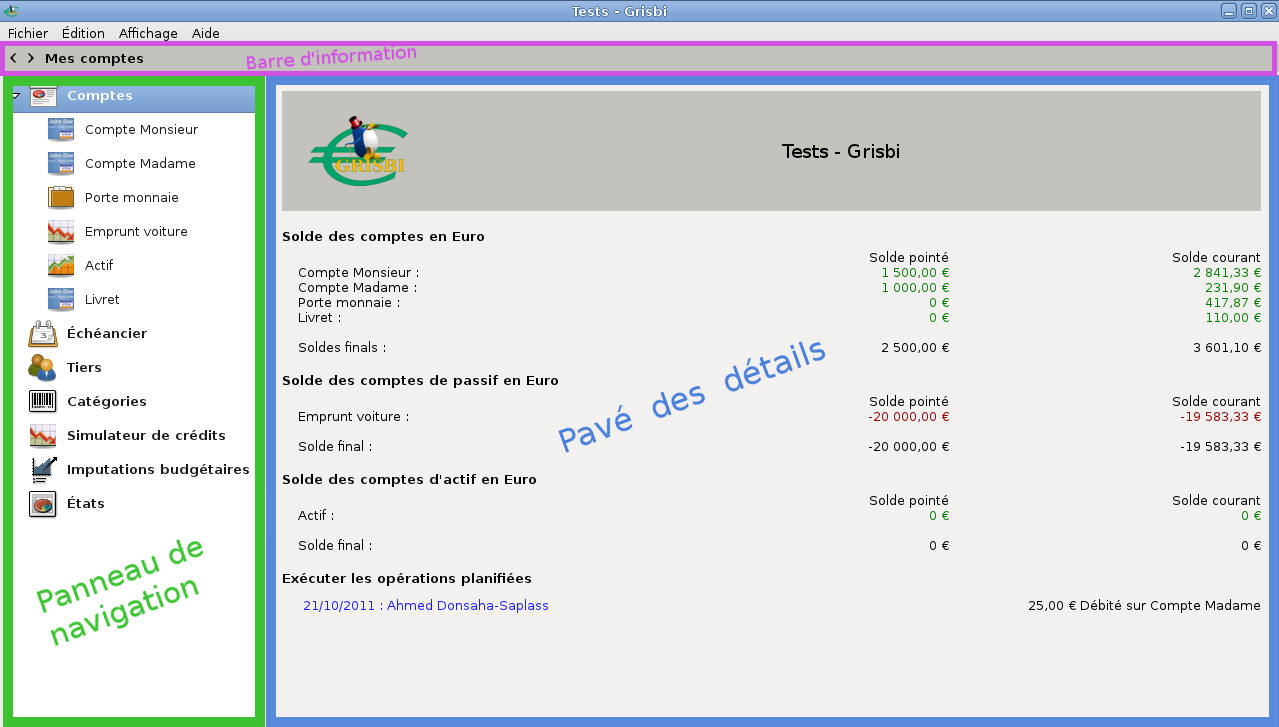
\includegraphics[scale=0.35]{image/screenshot/home}
\end{center}
\caption{Page d'accueil}
\label{home-img}
\end{figure}
% image centrée
\fi

% espace   : 5 mm
\vspacepdf{5mm}

Cette page affiche plusieurs pavés ;

\begin{itemize}
	 \item le pavé Nouveau, pour lancer l'assistant d'Aide à la création d'un nouveau fichier de comptes ;
	 \item le pavé Ouvrir, pour afficher un gestionnaire de fichier avec lequel vous pourrez chercher un fichier de comptes existant dans votre ordinateur ;
	 \item le pavé Importer, pour lancer l'assistant d'Aide à l'importation de fichiers ;
	 \item un ou plusieurs autres pavés, portant le nom de fichiers de comptes que Grisbi a déjà utilisés.
\end{itemize}

% espace   : 5 mm
\vspacepdf{5mm}

\textbf{Note} : les pavés portant les noms des fichiers de compte que Grisbi a déjà utilisés ne sont présents que si ces fichiers existent ; si vous voulez les enlever de cette page d'entrée, déplacez les dans un autre répertoire, ou supprimez-les.

% espace   : 5 mm
\vspacepdf{5mm}

En bas de page, un bandeau vous appelle à choisir une action en sélectionnant l'un de ces pavés.

% espace   : 5 mm
\vspacepdf{5mm}

Si vous voulez juste découvrir le logiciel Grisbi pour avoir un aperçu de son aspect et de ses possibilités, vous pouvez à la place utiliser un fichier exemple (voir la section \vref{new-example}).


CRÉER LA COPIE D'ÉCRAN DE LA PAGE ENTRÉE


%\section{Barre d'information\label{home-synthesis}}
%
%
%La barre d'information affiche le nom de l'onglet courant affiché, et peut afficher, complètement à droite, certains soldes en rapport avec ce qui est sélectionné dans le pavé des détails.
%
%% espace pour changement de thème
%\vspacepdf{5mm}
%Elle permet, en cliquant successivement sur l'un des deux petits triangles à sa gauche, de sélectionner l'un des onglets affichés dans le panneau de navigation  : \menu{Comptes}, \menu{Échéancier}, \menu{Tiers}, \menu{Simulateur de crédits}, \menu{Catégories}, \menu{Imputations budgétaires} et \menu{États}, et aussi l'un des sous-onglets des onglets \menu{Comptes} et \menu{États} s'ils sont déroulés dans le panneau de navigation.
%
%% Pas de commande au clavier pour cette fonction
%\textbf{Note} : ces triangles peuvent être remplacés, en fonction du thème de l'environnement de bureau ou du gestionnaire de fenêtres que vous utilisez, par d'autres caractères tels que +, -, >, <, etc.
%
%% espace pour changement de thème
%\vspacepdf{5mm}
%Le contenu de la sélection s'affiche dans le pavé des détails.
%
%% espace pour changement de thème
%\vspacepdf{5mm}
%Ces fonctionnalités peuvent être utilisées à la place de celles du panneau de navigation lorsque sa largeur est réduite à zéro et que l'on n'y a pas accès directement.
%
%
%\section{Panneau de navigation\label{home-accounting}}
%
%
%Le panneau de navigation affiche en caractères gras la liste des onglets : \menu{Comptes}, \menu{Échéancier}, \menu{Tiers}, \menu{Simulateur de crédits}, \menu{Catégories}, \menu{Imputations budgétaires} et \menu{États}. En cliquant sur le petit triangle noir à gauche des onglets \menu{Comptes} ou \menu{États}, on peut dérouler ou enrouler la liste de leurs sous-onglets. Vous pouvez changer l'ordre des onglets et des sous-onglets en cliquant sur l'un d'eux et en le déplaçant plus haut ou plus bas dans la liste.
%
%\textbf{Note} : ces triangles peuvent être remplacés, en fonction du thème de l'environnement de bureau ou du gestionnaire de fenêtres que vous utilisez, par d'autres caractères tels que +, -, >, <, etc.
%
%% espace pour changement de thème
%\vspacepdf{5mm}
%Vous pouvez sélectionner un de ces onglets ou sous-onglets en cliquant sur son nom. Vous pouvez aussi déplacer la sélection dans cette liste d'onglets et de sous-onglets avec les touches du clavier \key{Flèche Haut}, \key{Flèche Bas}, \key{Page Haut} ou \key{Page Bas}, ou avec la molette de la souris. 
%
%% espace pour changement de thème
%\vspacepdf{5mm}
%Le contenu de la sélection s'affiche dans le pavé des détails. 
%
%% espace pour changement de thème
%\vspacepdf{5mm}
%On peut réduire ou agrandir la largeur du panneau de navigation en cliquant sur la fine barre verticale entre ce panneau et le pavé des détails, et en la déplaçant. Si la largeur du panneau a été réduite à zéro, ou agrandie au maximum de la largeur de la fenêtre de Grisbi, il faut retrouver cette barre, respectivement complètement à gauche ou à droite de la fenêtre, et la faire glisser à la place désirée. 
%
%% espace pour changement de thème
%\vspacepdf{5mm}
%Des \indexword{menus contextuels}\index{menu contextuel}, accessibles par un clic-droit de souris, sont disponibles sur les éléments de ce panneau et proposent les fonctions suivantes :
%
%\begin{itemize}
%	 \item sur \menu{Comptes} :
%		\begin{itemize}
%			 \item \menu{Nouveau compte} ;
%		\end{itemize}
%	 \item sur un compte quelconque : 
%		\begin{itemize}
%			 \item \menu{Nouveau compte},
%			 \item \menu{Supprimer ce compte} ;
%		\end{itemize}
%	 \item sur \menu{Tiers} :
%		\begin{itemize}
%			 \item \menu{Nouveau tiers},
%			 \item \menu{Supprimer le tiers sélectionné},
%			 \item \menu{Éditer le tiers sélectionné},
%			 \item \menu{Gérer les tiers},
%			 \item \menu{Supprimer les tiers inutilisés} ;
%		\end{itemize}
%	 \item sur \menu{Catégories} : 
%		\begin{itemize}
%			 \item \menu{Nouvelle catégorie},
%			 \item \menu{Supprimer la catégorie sélectionnée},
%			 \item \menu{Editer la catégorie sélectionnée},
%			 \item \menu{Importer un fichier de catégories (.csgb)},
%			 \item \menu{Exporter la liste des catégories (.csgb)} ;
%		\end{itemize}
%	 \item sur \menu{Imputations budgétaires} :
%		\begin{itemize}
%			 \item \menu{Nouvelle imputation budgétaire},
%			 \item \menu{Supprimer l'imputation sélectionnée},
%			 \item \menu{Editer l'imputation sélectionnée},
%			 \item \menu{Importer un fichier d'imputations budgétaires (.isgb)},
%			 \item \menu{Exporter la liste des imputations budgétaires (.isgb)} ;
%		\end{itemize}
%	 \item sur \menu{État} : \menu{Nouvel état} ;
%	 \item sur un état quelconque : 
%		\begin{itemize}
%			 \item \menu{Nouvel état},
%			 \item \menu{Supprimer cet état}.
%		\end{itemize}
%\end{itemize}
%
%\ifIllustration
%\else
%% saut de page pour titre solidaire
%\newpage
%\fi
%
%
%\section{Pavé des détails\label{home-details}}
%
%
%Le pavé des détails affiche tous les détails sur les onglets ou sous-onglets sélectionnés par la barre d'information ou le panneau de navigation. C'est la zone de travail principale de Grisbi.
%
%On peut réduire ou agrandir sa largeur en cliquant sur la fine barre verticale entre ce pavé et le panneau de navigation, et en la déplaçant. Si la largeur du pavé a été réduite à zéro ou agrandie au maximum de la largeur de la fenêtre de Grisbi, il faut retrouver cette barre, respectivement complètement à droite ou à gauche de la fenêtre, et la faire glisser à la place désirée. 
% 
% 
%\subsection{Affichage de la page d'accueil\label{home-details-homepage}}
%
%Pour afficher la page d'accueil, sélectionnez l'onglet \menu{Comptes} ; le pavé des détails affiche, de haut en bas :
%
%\begin{itemize}
%	 \item dans un pavé sur fond gris, l'icône \menu{Grisbi} à gauche, et à droite un \indexword{titre}\index{affichage !titre}\index{titre !page d'accueil} qui permet d'identifier sur quelle comptabilité vous travaillez actuellement, sous la forme \og libellé - Grisbi\fg{} ; vous pouvez définir ce libellé, parmi trois possibilités, dans le menu \menu{Édition - Préférences} (voir le paragraphe \vref{setup-display-addresses-titles}, \menu{Titres}) :
%		\begin{itemize}
%			 \item l'\menu{Entité comptable} : c'est le nom du domaine de comptabilité sur lequel vous travaillez, par exemple \og Ma comptabilité \fg{} ou \og Association \fg{}, et que vous avez saisi à la création du fichier de comptes ; vous pouvez le modifier ici dans le champ \menu{Nom de l'entité comptable} ; cela peut être utile si vous gérez plusieurs \indexword{entités comptables}\index{entité comptable}, 
%			 \item le \menu{Titulaire du compte} : c'est le nom du titulaire (ou du propriétaire) du dernier compte consulté ; si le titulaire n'est pas renseigné dans les propriétés du compte, Grisbi affiche le nom de ce compte,
%			 \item le \menu{Nom du fichier de comptes} : c'est le nom du fichier dans le répertoire courant, sous la forme \file{nom\_de\_\_votre\_fichier.gsb}, et c'est le choix par défaut ;
%		\end{itemize}
%	 \item pour chaque devise séparément, pour tous les comptes et \indexword{groupes de comptes}\index{groupe de comptes}, sous les libellés \menu{Solde rapproché} et \menu{Solde courant} :
%		\begin{itemize}
%			 \item le solde des comptes bancaires et comptes de caisse, le solde partiel des groupes de comptes et leur solde final,
%% saut de ligne pour indentation correcte de la note dans la liste
%
%			 \textbf{Note} : vous pouvez ajuster l'ordre d'affichage des soldes partiels des groupes de comptes (voir le paragraphe \vref{setup-general-home-partBalance}, \menu{Soldes partiels de la liste des comptes}).			 
%			 \item le solde des comptes de passif et leur solde final,
%			 \item le solde des comptes d'actif et leur solde final ;
%		\end{itemize}
%	\item les \indexword{alertes des opérations planifiées}\index{alerte !opération planifiée} à échéance ou clôturées, avec leurs date, libellé et montant, selon les choix faits dans le menu \menu{Édition - Préférences} (voir la section \vref{setup-general-planned}, \menu{Échéancier}) ;
%	\item la liste des comptes dont le solde est passé sous le \menu{Solde minimal autorisé} ;
%	\item la liste des comptes dont le solde est passé sous le \menu{Solde minimal voulu}.
%\end{itemize}
%
%% espace avant Attention ou Note  : 5 mm
%\vspacepdf{5mm}
%
%\textbf{Note} : pour les définitions du \menu{Solde minimal autorisé} et du \menu{Solde minimal voulu}, voir la section \vref{accounts-properties}, \menu{Propriétés d'un compte}.
%
%% espace pour changement de thème
%\vspacepdf{5mm}
%Les libellés des comptes s'affichent en noir{\couleur} ; au passage du pointeur de la souris sur la ligne de l'un d'eux, cette couleur passe au gris{\couleur}.
%Un solde supérieur au \menu{Solde minimal voulu} s'affiche en vert foncé{\couleur} ; au passage du pointeur sur sa ligne, cette couleur passe au vert clair{\couleur}.
%Un solde inférieur au \menu{Solde minimal voulu} et supérieur au \menu{Solde minimal autorisé} s'affiche en orange{\couleur} ; au passage du pointeur sur sa ligne, cette couleur passe à l'orange clair{\couleur}.
%Un solde inférieur au \menu{Solde minimal autorisé} s'affiche en rouge{\couleur} ; au passage du pointeur sur sa ligne, cette couleur passe au rouge clair{\couleur}.
%
%Au passage du pointeur de la souris sur la ligne d'un compte, tout changement de couleur indique que si l'on clique (droit ou gauche) avec la souris, ce compte s'affiche, comme s'il avait été sélectionné avec la barre d'information ou le panneau de navigation ; il affiche alors la page qui contient la ligne d'opération  affichant ce solde.
%
%Un solde partiel, qui correspond à un groupe de comptes, s'affiche en noir{\couleur}. S'il est négatif, il peut s'afficher en rouge foncé{\couleur}, mais seulement si cela a été configuré ainsi (voir le paragraphe \vref{setup-general-home-partBalance}, \menu{Soldes partiels de la liste des comptes}). Une ligne de solde partiel ne change pas de couleur au passage du pointeur de la souris dessus, car on ne peut pas afficher les opérations d'un groupe de comptes.
%
%% espace pour changement de thème
%\vspacepdf{5mm}
%Vous pouvez configurer certains aspects de l'affichage de cette page d'accueil dans le menu \menu{Édition - Préférences} ou dans l'onglet \menu{Propriétés} de chaque compte :
%\begin{itemize}
%	 \item \menu{\indexword{Polices}\index{polices}, \indexword{logo}\index{logo} et \indexword{couleurs}\index{couleurs}} : section \vref{setup-display-logo} ;
%	 \item \menu{Titres} : section \vref{setup-display-addresses-titles} ;
%	 \item \menu{Calcul des soldes} : paragraphe \vref{setup-general-home-balance} ;
%	 \item \menu{Soldes partiels de la liste des comptes} : paragraphe \vref{setup-general-home-partBalance} ;
%	 \item \menu{Alertes de l'échéancier} : section \vref{setup-general-planned} ;
%	 \item comptes sous le \menu{\indexword{Solde minimal autorisé}}\index{solde !minimal autorisé} : section \vref{accounts-properties} ;
%	 \item comptes sous le \menu{\indexword{Solde minimal voulu}}\index{solde !minimal voulu} : section  \vref{accounts-properties}.
%\end{itemize}
%
%En particulier, si vous trouvez une erreur d’orthographe dans cette page, vous pourrez la corriger : voir le paragraphe \vref{setup-general-home-final}, \menu{Pluriel de final} !
%
%\ifIllustration
%% saut de page pour paragraphe solidaire
%\newpage
%\fi
%
%\section{Barre de menus\label{home-menus}}
%
%
%Comme dans de nombreuses applications graphiques, la plupart des fonctionnalités importantes de Grisbi sont accessibles au moyen des menus de la \indexword{barre de menus}\index{barre de menus}. Nous détaillons ici leurs fonctionnalités.
%
%
%\subsection{Menu \menu{Fichier}\label{home-menus-file}}
%
%Ce menu comprend les fonctions suivantes :
%
%\begin{itemize}
%	\item \menu{Nouveau fichier de comptes} : crée un nouveau fichier de comptes ; le fichier courant est donc fermé et un nouveau fichier vide est créé avec un compte vide (raccourci-clavier \key{Ctrl}\key{N}), voir la section \vref{start-newfile} ; à ne pas confondre avec la création d'un nouveau compte ;
%	\item \menu{Ouvrir} : ouvre un fichier de comptes (raccourci-clavier \key{Ctrl}\key{O}) ;
%	\item \menu{Derniers fichiers} : affiche la liste des n derniers fichiers ouverts avec Grisbi (seulement s'il y en a eu plusieurs) ; ce nombre est configurable dans le menu \menu{Edition - Préférences}, voir la section \vref{setup-general-files-manage}, \menu{Gestion des fichiers de compte} ;
%	\item \menu{Enregistrer} : enregistre le fichier de comptes en cours (raccourci-clavier \key{Ctrl}\key{S}) ;
%	\item \menu{Enregistrer sous} : ouvre un gestionnaire de fichiers pour enregistrer le fichier de comptes en cours avec le nom et à l'emplacement de 	votre choix ; Grisbi vous propose par défaut le répertoire courant, le nom du fichier de comptes en cours, avec l'extension \file{.gsb} ;
%	\item \menu{Importer un fichier} : démarre l'assistant d'importation de fichiers d'un autre logiciel ; voir la section \vref{move-import-importinit} ;
%	\item \menu{Exporter vers un fichier QIF/CSV} : démarre l'assistant d'exportation de fichiers de compte ; voir la section \vref{move-export} ;	
%	\item \menu{Créer une archive} : démarre l'assistant de création d'archive ; voir la section \vref{datamanagement-history-new} ;	
%	\item \menu{Exporter une archive vers un fichier GSB/QIF/CSV} : démarre l'assistant d'exportation d'archive ; voir la section \vref{datamanagement-history-export} ;
%	\item \menu{Déboguer le fichier de compte} : démarre l'assistant de 	débogage de ce fichier, qui va vous aider à chercher des incohérences dans votre fichier de comptes ; voir la section \vref{maintenance-file-debug} ;
%	\item \menu{Rendre anonyme le fichier de comptes} : démarre l'assistant qui produit une copie anonymée de votre fichier de comptes ; ce fichier pourra être joint à un rapport de bogue ; voir la section \vref{maintenance-file-anonymous} ;	
%	\item \menu{Rendre anonyme le fichier QIF} : démarre l'assistant qui produit une copie anonymée de ce fichier ; ce fichier pourra être joint à un rapport de bogue ; voir la section \vref{maintenance-QIF-anonymous} ;	
%	\item \menu{Mode de débogage} : met Grisbi en mode de débogage, qui crée un fichier-journal des évènements ; voir la section \vref{maintenance-debug-mode} ; 	
%	\item \menu{Fermer} : ferme le fichier de comptes en cours ; Grisbi vous propose de l'enregistrer si ce n'est déjà fait (raccourci-clavier \key{Ctrl}\key{W}) ;
%	\item \menu{Quitter} : ferme Grisbi ; Grisbi vous propose auparavant d'enregistrer le fichier de comptes, si ce n'est pas déjà fait (raccourci-clavier \key{Ctrl}\key{Q}).
%\end{itemize}
%
%
%\subsection{Menu \menu{Édition}\label{home-menus-edit}}
%
%Ce menu comprend les fonctions suivantes :
%
%\begin{itemize}
%	\item \menu{Editer l'opération} : voir la section \vref{transactions-modify}, \menu{Modification d'une opération} ;
%	\item \menu{Nouvelle opération} : voir la section \vref{transactions-new}, \menu{Saisie d'une nouvelle opération} ;
%	\item \menu{Supprimer une opération} : voir la section \vref{transactions-delete}, \menu{Suppression d'une opération} ;
%	\item \menu{Utiliser l'opération sélectionnée comme modèle} : voir la section \vref{transactions-model}, \menu{Opération sélectionnée comme modèle} ;
%	\item \menu{Cloner l'opération} : voir la section \vref{transactions-duplicate}, \menu{Clonage d'une opération} ;
%	\item \menu{Convertir en opération planifiée} : voir la section \vref{transactions-schedule}, \menu{Conversion d'une opération en opération planifiée} ;
%	\item \menu{Déplacer l'opération vers un autre compte} : voir la section \vref{transactions-move}, \menu{Déplacement d'une opération vers un autre compte} ;
%	\item \menu{Nouveau compte} : voir la section \vref{accounts-new}, \menu{Création d'un nouveau compte} ;
%	\item \menu{Supprimer le compte courant} : voir la section \vref{accounts-delete}, \menu{Suppression d'un compte} ;
%	\item \menu{Préférences} : permet de configurer Grisbi ; voir le chapitre \vref{setup}, \menu{Configuration de Grisbi}.
%\end{itemize}
%
%
%\subsection{Menu \menu{Affichage}\label{home-menus-display}}
%
%Ce menu comprend les fonctions suivantes : 
%
%\begin{itemize}
%	 \item \menu{Montrer le formulaire de saisie d'opérations} ; 
%	 \item \menu{Montrer les opérations rapprochées} (raccourci-clavier \key{Alt}\key{R}) ;
%	 \item \menu{Montrer les lignes d'archives} (raccourci-clavier \key{Altl}\key{L}) ;
%	 \item \menu{Montrer les \indexword{comptes clos}}\index{compte !clos} ;
%	 \item \menu{Montrer une ligne par opération} ;
%	 \item \menu{Montrer deux lignes par opération} ;
%	 \item \menu{Montrer trois lignes par opération} ;
%	 \item \menu{Montrer quatre lignes par opération} ;
%	 \item \menu{Réinitialiser la largeur des colonnes} ; permet de remettre les colonnes des listes d'opérations à leur largeur d'origine.
%\end{itemize}
%
%
%\subsection{Menu \menu{Aide}\label{home-menus-help}}
%
%La plupart des choix de ce menu donnent accès à des sites Web. Pour que ces accès fonctionnent, il faut avoir indiqué à Grisbi le logiciel de navigation (ou navigateur) que vous souhaitez utiliser, dans le menu \menu{Édition - Préférences} (voir la section \vref{setup-general-programs}, \menu{Programmes}). Le menu \menu{Aide} comprend les choix suivants :
%
%\begin{itemize}
%	\item \menu{Manuel} : ouvre votre navigateur à la page \og Manuel de l'Utilisateur de Grisbi \fg{} (raccourci-clavier \key{Ctrl}\key{H}) ;
%	\item \menu{Démarrage rapide} : ouvre votre navigateur à la page \og Démarrage Rapide de Grisbi \fg{} ;
%	\item \menu{Traduction} : ouvre votre navigateur à la page \og Traduire Grisbi \fg{}, pour vous inviter à nous aider à l'élargissement de 	l'internationalisation de Grisbi ;
%	\item \menu{À propos de Grisbi} : affiche la boîte d'information sur l'application : vous y trouverez des détails sur la version, le lien vers le site de Grisbi, les remerciements (contributeurs au projet) et la licence d'utilisation ;
%	\item \menu{Site Web de Grisbi} : ouvre votre navigateur à la page du site de \lang{Grisbi}\footnote{\urlGrisbi{}} ;
%	\item \menu{Signaler une anomalie} : ouvre votre navigateur à la page du \lang{traqueur de bogues de Grisbi}\footnote{\urlBugTracker{}} pour vous permettre de signaler un bogue que vous auriez découvert. Vous pouvez également suivre sur cette page l'évolution des corrections apportées aux bogues signalés ;
%	\item \menu{Astuce du jour} : ouvre une boîte de dialogue qui affiche une astuce d'utilisation, différente à chaque démarrage de Grisbi ; vous pouvez y 	afficher successivement toutes les astuces, et choisir ou non l'affichage de 	l'astuce du jour au démarrage de Grisbi. Pour supprimer ou réactiver l'astuce du 	jour, voir le paragraphe \vref{setup-display-messages-trick}, \menu{Astuce du jour}.
%\end{itemize}
%
%
%\section{Raccourcis-clavier\label{home-shortcuts}}
%
%
%Les raccourcis-clavier facilitent la saisie des données et la navigation dans les fenêtres de Grisbi, en évitant le recours systématique au déplacement et au clic de la souris. En utilisant ceux correspondant aux manipulations les plus courantes pour vous, vous améliorez votre \indexword{ergonomie}\index{ergonomie} en limitant les mouvements importants de vos bras.
% 
%Grisbi dispose d'un certain nombre de raccourcis-clavier, présentés ici selon différents thèmes (voir aussi la section \vref{introduction-manual-conventions}, \menu{Conventions typographiques du présent manuel}).
%
%
%\subsection{Application et fichiers}
%
%\begin{itemize}
%	\item Nouveau fichier de comptes : \key{Ctrl}\key{N}
%	\item Ouvrir un fichier de comptes : \key{Ctrl}\key{O}
%	\item Enregistrer le fichier de comptes : \key{Ctrl}\key{S}
%	\item Fermer le fichier de comptes : \key{Ctrl}\key{W}
%	\item Fermer Grisbi : \key{Ctrl}\key{Q}
%\end{itemize}
%
%
%\subsection{Panneau de navigation}
%
%\begin{itemize}
%	\item Sélectionner un onglet ou un compte : \key{Flèche Haut}, \key{Flèche Bas}, \key{Page Haut} ou \key{Page Bas}
%\end{itemize}
%
%
%\subsection{Liste des opérations et des opérations planifiées}
%
%\begin{itemize}
%	\item Sélectionner une opération : \key{Entrée}
%	\item Déplacer la sélection : \key{Flèche Haut} ou \key{Flèche Bas}
%	\item Nouvelle opération : \key{Entrée} sur ligne vide, ou \key{Ctrl}\key{T}
%	\item Modifier une opération : \key{Entrée}
%	\item Supprimer une opération : \key{Suppr} ;
%	\item Pointer ou dépointer une opération : \key{Ctrl}\key{P}
%	\item Rapprocher ou dérapprocher une opération : \key{Ctrl}\key{R}
%	\item Montrer ou masquer les opérations rapprochées :  \key{Alt}\key{R}
%	\item Montrer ou masquer les lignes d'archives : \key{Altl}\key{L}
%\end{itemize}
%
%
%\subsection{Formulaire de saisie }
%
%\begin{itemize}
%	\item La touche \key{Entrée} est configurable : elle permet soit de se déplacer dans le formulaire de saisie, soit de valider l'entrée
%	\item Se déplacer au champ suivant : \key{Tabulation} (selon votre choix de configuration)
%	\item Annuler la saisie en cours : \key{Échap}
%	\item Accepter l'auto-complètement : \key{Tabulation} ou \key{Entrée} (selon votre choix de configuration)
%	\item  Symbole de l'euro : \key{AltGr}\key{e}
%\end{itemize}
%
%
%\subsection{Listes déroulantes}
%
%\begin{itemize}
%	 \item Ouvrir une liste : \key{Page Bas} ou \key{Flèche bas}
%	 \item Se déplacer dans la liste : \key{Flèche haut}, \key{Flèche bas}, \key{Page Haut} ou \key{Page Bas}
%	 \item Valider un choix à l'intérieur d'une liste : \key{Entrée}
%	 \item Devises, exercices et modes de règlement :
%		\begin{itemize}
%			\item ouvrir la liste : \key{Espace} ; 
%			\item se déplacer dans la liste : \key{Flèche Haut} ou \key{Flèche Bas} ;
%			\item valider l'item de la liste : \key{Espace}.
%		\end{itemize}
%\end{itemize}
%
%
%\subsection{Dates saisies au calendrier}
%
%\begin{itemize}
%	\item Ouvre un calendrier (sur le champ de date) : \key{Ctrl}\key{Entrée}
%	\item Ferme le calendrier sans modifier la date : \key{Échap}
%	\item Valide la date sélectionnée : \key{Entrée}
%	\item Jour suivant ou précédent : \key{+} ou \key{-}, \key{Flèche Droite} ou \key{Flèche Gauche}
%	\item Semaine précédente ou suivante : \key{Flèche Haut} ou \key{Flèche Bas}
%	\item Mois précédent ou suivant : \key{Page Haut} ou \key{Page Bas}
%	\item Premier jour ou dernier jour du mois : \key{Début} ou \key{Fin}
%\end{itemize}
%
%
%\subsection{Dates saisies au clavier}
%
%\begin{itemize}
%	\item Jour suivant ou précédent : \key{+} ou \key{-}
%	\item Semaine précédente ou suivante : \key{Majuscule} \key{+} ou \key{Majuscule} \key{-}
%	\item Mois précédent ou suivant : \key{Page Haut} ou \key{Page Bas}
%	\item Année précédente ou suivante : \key{Majuscule} \key{Page Haut} ou \key{Majuscule} \key{Page Bas}
%	\item Valide la date sélectionnée \key{Entrée}
%\end{itemize}
%
%
%\subsection{Tiers, catégories, imputations budgétaires, simulateur de crédits, données historiques et prévisions}
%
%\begin{itemize}
%	\item Déplacer la sélection : \key{Flèche Haut}, \key{Flèche Bas}, \key{Page Haut} ou \key{Page Bas}
%%Ces raccourcis ne fonctionnent plus :
%%	\item afficher les sous-catégories ou sous-imputations budgétaires (sur une catégorie ou une imputation budgétaire) : \key{Espace} ;
%%	\item afficher les opérations des sous-catégories ou sous-imputations budgétaires (sur une sous-catégorie ou une sous-imputation budgétaire) : \key{Espace}.
%\end{itemize}
%
%
%\subsection{États et Configuration}
%
%\begin{itemize}
%	\item Sélectionner un autre onglet : \key{Flèche Haut}, \key{Flèche Bas}, \key{Page Haut}, \key{Page Bas}
%	\item Naviguer entre le panneau des onglets et les différentes options du panneau des réglages : \key{Tabulation}, \key{Flèche Haut}, \key{Flèche Bas}, \key{Flèche Gauche} et \key{Flèche Droit}
%\end{itemize}
%
%\subsection{Aide}
%
%\begin{itemize}
%	\item Ouvre votre navigateur à la page du Manuel de l'Utilisateur de Grisbi \key{Ctrl}\key{H}
%\end{itemize}














\myclearemptydoublepage



%%%%%%%%%%%%%%%%%%%%%%%%%%%%%%%%%%%%%%%%%%%%%%%%%%%%%%%%%%%%%%%%%
% Contents : The first start chapter
% $Id : grisbi-manuel-start.tex, v 0.4 2002/10/27 Daniel Cartron
% $Id : grisbi-manuel-start.tex, v 0.5.0 2004/06/01 Loic Breilloux
% $Id : grisbi-manuel-start.tex, v 0.6.0 2011/11/17 Jean-Luc Duflot
% $Id : grisbi-manuel-start.tex, v 0.8.9 2012/04/27 Jean-Luc Duflot
% $Id : grisbi-manuel-start.tex, v 1.0 2014/02/12 Jean-Luc Duflot
%%%%%%%%%%%%%%%%%%%%%%%%%%%%%%%%%%%%%%%%%%%%%%%%%%%%%%%%%%%%%%%%%


\chapter{Premier démarrage de Grisbi\label{start}}


\section{Assistant premier démarrage\label{start-first}}


Au premier démarrage de Grisbi, l'assistant premier démarrage s'affiche pour
vous aider à configurer l'application. Il comprend deux étapes, qui concernent
la gestion du \indexword{fichier de comptes}\index{fichier de comptes} (chargement et enregistrement automatiques,
chiffrement et copies de sauvegarde).

Il est conseillé de cocher les options :

\begin{itemize}
 \item chargement automatique du dernier fichier consulté ;
 \item enregistrer automatiquement en fermant ;
 \item effectuer une copie de sauvegarde avant d'enregistrer le fichier.
\end{itemize}

Cet assistant est suivi automatiquement par un deuxième, l'assistant de création du \indexword{fichier de comptes}\index{fichier de comptes}. Puis vient automatiquement un troisième assistant, l'assistant de création de compte, qui permet de créer le premier compte. Tout cela est décrit en détail dans la section \ref{start-newfile} ci-dessous.

À tout moment vous pouvez sortir de n'importe quel assistant par le bouton \menu{Annuler}.

Si vous ne voulez pas utiliser l'assistant premier démarrage, vous pouvez à la
place utiliser un fichier exemple (voir la section ci-dessous).


\section{Fichier exemple\label{start-example}}


Si vous voulez utiliser Grisbi immédiatement sans être obligé de rentrer tout un tas d'opérations, par exemple  pour vous faire une idée des possibilités de ce logiciel, vous pouvez télécharger le fichier \file{Example\_1.0.gsb}, soit sur le site de Grisbi dans la rubrique Téléchargement{\siteGrisbiTelechargement}, soit sur le site {Sourceforge}{\siteSourceForgeDocumentation}.

% espace avant Attention ou Note  :  mm
\vspacepdf{3mm}
\textbf{Note} : dans ce fichier exemple, les noms des tiers sont de pure invention ; seul un hasard indépendant de notre volonté peut avoir fait que ce soit celui d'une personne ou d'une entité existante.


\section{Création d'un nouveau fichier de comptes\label{start-newfile}}


La première fois que vous utiliserez Grisbi, vous devrez d'abord créer un \indexword{fichier
de comptes}\index{fichier de comptes}. L'\gls{extension} de ce fichier sera \file{.gsb} et son nom \file{nom-de-votre-fichier.gsb}. 

Immédiatement après, il vous faudra créer au minimum un compte, et par la suite quelques autres comptes (comptes courants, d'épargne, de crédit, éventuellement un compte d'espèces et quelques comptes de transition) qui contiendront leurs opérations respectives. 

Pour une gestion familiale, vous n'aurez normalement qu'un seul fichier de comptes, car cela permet tous les échanges entre vos différents comptes. Si vous gérez une association, ou une autre famille sans rapport comptable avec la première, vous créerez un autre fichier de comptes, qui portera un autre nom \file{nom-de-votre-deuxième-fichier.gsb}. Ainsi les \indexword{entités comptables}\index{entité comptable} resteront bien séparées.

% espace avant Attention ou Note  : 5 mm
\vspacepdf{5mm}
\strong{Attention} : pour une entité comptable donnée, il est nécessaire et important de bien distinguer LE \og \indexword{fichier de comptes}\index{fichier de comptes} \fg{} et LES \og \indexword{fichiers de compte}\index{fichiers de compte} \fg{} :

\begin{itemize}
	\item LE \og fichier de comptes \fg{} que vous aurez créé aura pour extension \file{.gsb} et pour nom \file{nom-de-votre-fichier.gsb} ; il contient toutes les données de tous les comptes créés pour la gestion d'une entité comptable ;
	\item LES \og fichiers de compte \fg{} sont des fichiers que vous pourriez être amené(e) à utiliser ou à créer pour importer ou exporter des données d'une application de comptabilité à une autre ; ces fichiers ne contiendront que les données d'un seul compte (courant ou autre) à la fois ; ils auront des extensions différentes (\file{.ofx}, \file{.csv} ou \file{.qif}) suivant leur contenu ; pour plus de détails, voir le chapitre \vref{move}, \menu{Export et import de comptes}.
\end{itemize}

% espace après Attention ou Note  : 5 mm
\vspacepdf{5mm}
Autrement dit, l'ensemble des comptes de votre foyer est enregistré dans un fichier de comptes, et l'ensemble des comptes de votre association l'est dans un autre fichier de comptes ; et un compte dans Grisbi peut correspondre à un fichier de compte, mais seulement lorsqu'on parle d'importation ou d'exportation de données.

% espace pour changement de thème
\vspacepdf{5mm}
Le déroulement général de la procédure de création d'un fichier de comptes est le suivant : cliquez sur le menu \menu{Fichier - Nouveau fichier de comptes} ; l'assistant de création de fichier de comptes s'ouvre, qui comprend six étapes. À la sixième étape, l'assistant vous propose :

\begin{itemize}
	\item  soit de créer un nouveau compte, et il enchaîne sur l'assistant de création de compte, qui comprend lui-même cinq étapes, pour créer le premier compte (car il est indispensable de disposer d'au moins un compte) ;
	\item soit d'utiliser des données déjà existantes, et il enchaîne alors sur l'assistant d'importation des opérations, qui comprend aussi cinq étapes, pour importer des opérations de comptes existants.
\end{itemize}

Après la création de ce premier compte ou l'importation d'opérations de comptes existants, si vous voulez créer d'autres comptes, vous retournerez à la fin de la procédure de création du fichier de comptes, ce qui vous renverra dans les deux cas vers la création d'un nouveau compte.

% espace pour changement de thème
\vspacepdf{5mm}
Pour créer votre fichier de comptes, cliquez sur le menu \menu{Fichier - Nouveau fichier de comptes} ; la procédure détaillée est la suivante :

\begin{enumerate}
	\item fenêtre d'accueil : validez par le bouton \menu{Suivant} ;
	\item configuration
		\ifIllustration générale\refimage{start-file-create-img} :
		\else générale :
		\fi

		\ifIllustration
		% image centrée
		\begin{figure}[htbp]
		\begin{center}
		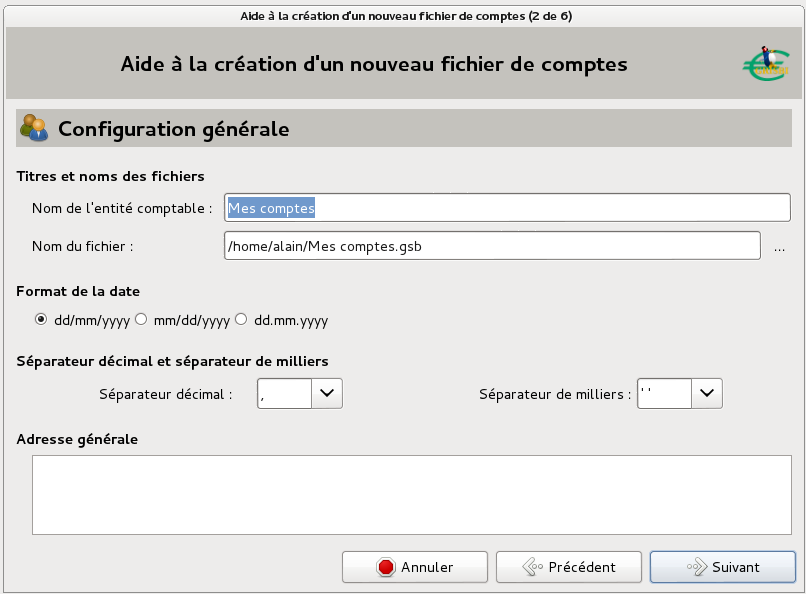
\includegraphics[scale=0.5]{image/screenshot/start_file_create}
		\end{center}
		\caption{Configuration générale du fichier de comptes}
		\label{start-file-create-img}
		\end{figure}
		% image centrée
		\fi
		
		\begin{enumerate} 
		 	\item choisissez le nom de l'entité comptable dont vous gérez la comptabilité, par exemple \og Ma comptabilité \fg{}, qui pourra être choisi comme titre de la page d'accueil de l'application Grisbi,
			\item saisissez le nom du fichier de comptes avec son arborescence complète ; Grisbi vous propose par défaut le même nom que celui de l'entité comptable, mais vous pouvez le modifier,
			\item cochez la case \menu{Chiffrer le fichier Grisbi} si vous voulez \gls{chiffrer} le fichier de comptes,
			\item sélectionnez le \indexword{format de la date}\index{format de date} avec l'un des deux boutons : dd/mm/yyyy pour jour/mois/année, ou mm/dd/yyyy pour mois/jour/année,
			\item choisissez le \indexword{séparateur}\index{séparateur} décimal et celui des milliers dans les listes déroulantes,
			 \item renseignez l'adresse (facultatif),
			 \item  validez par le bouton \menu{Suivant} ;
		\end{enumerate}
		
	\item sélection de la \indexword{devise}\index{devise} de base :
		\begin{enumerate} 
		 	\item cliquez sur la devise choisie dans la liste,
			\item cochez la case \menu{Afficher les devises obsolètes} si vous voulez aussi afficher d'anciennes devises,
			\item validez par le bouton \menu{Suivant} ;
		\end{enumerate}
	\item sélection des \indexword{types de catégories}\index{catégories !types} utilisées :
		\begin{enumerate} 
		 	\item cliquez sur la catégorie choisie dans la liste, qui comprend : \menu{Catégories générales}, \menu{Liste vide}, \menu{Comptabilité libérale}, \menu{Plan comptable associatif simplifié} et \menu{Plan comptable associatif},
			\item cochez la case \menu{Afficher l'ensemble des catégories} si vous voulez aussi afficher d'autres catégories libellées en anglais,
			\item validez par le bouton \menu{Suivant} ;
		\end{enumerate}		

	\item définition des \indexword{banques}\index{banques !définition} détenant vos comptes :
		\begin{enumerate} 
		 	\item cliquez sur  \menu{Ajouter} pour définir une banque ; renseignez les détails de la banque (nom, code banque, etc.), puis validez par le bouton \menu{Ajouter} pour valider la banque,
			\item sélectionnez une banque dans la liste et validez par le bouton \menu{Enlever} pour supprimer une banque, puis confirmez dans la fenêtre qui s'ouvre,
			\item répétez les actions a et b autant de fois que nécessaire,
			\item  validez par le bouton \menu{Suivant} pour passer à l'étape suivante, \menu{Création d'un nouveau compte} ;
		\end{enumerate}		 	

	\item configuration terminée  : la configuration du fichier de comptes est terminée, et cette fenêtre vous propose de choisir l'une des deux méthodes de création de votre premier
\ifIllustration compte\refimage{start-account-choice-img} :
\else compte :
\fi

\ifIllustration
% image centrée
\begin{figure}[ht]
\begin{center}
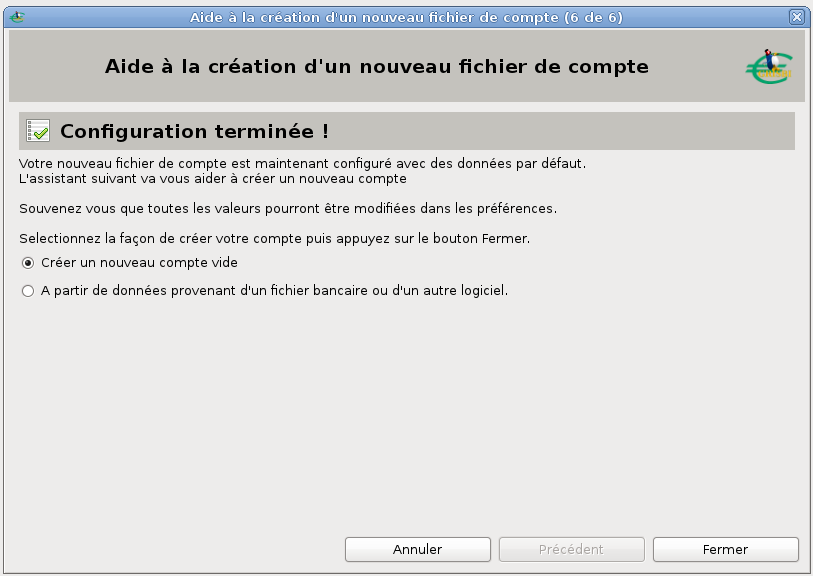
\includegraphics[scale=0.5]{image/screenshot/start_account_choice}
\end{center}
\caption{Choix du premier compte}
\label{start-account-choice-img}
\end{figure}
% image centrée
\fi

		\begin{itemize}
			\item \menu{Créer un nouveau compte vide} : si vous cochez cette ligne, puis si vous validez par le bouton \menu{Fermer}, cette fenêtre se ferme et l'assistant de création de nouveau compte démarre. Reportez-vous à la section \vref{accounts-new}, \menu{Création d'un nouveau compte}, qui décrit entièrement cette procédure, puis revenez à cette page ;

			\item \menu{À partir de données provenant d'un fichier bancaire ou d'un autre logiciel} : si vous cochez cette ligne, puis si vous validez par le bouton \menu{Fermer}, cette fenêtre se ferme et l'assistant d'importation des données d'un fichier de compte par Grisbi démarre. Reportez-vous à la section \vref{move-import-importinit}, \menu{Import de fichiers de compte d'un autre logiciel dans Grisbi}, qui décrit entièrement cette procédure, puis revenez à cette page.
		\end{itemize}
\end{enumerate}

% étiquette du paragraphe suivant, pour que les liens hypertexte dans account.tex et QIF.tex  arrivent bien dessus
\label{start-newfile-end}

\textit{\textbf{D'une manière ou d'une autre}}, vous venez donc de créer votre fichier de comptes, ainsi que le premier compte de ce fichier. 

%espace pour changement de thème
\vspacepdf{5mm}
Si vous voulez créer maintenant d'autres comptes, sélectionnez le menu \menu{Édition - Nouveau compte} pour créer un autre compte (voir la section \vref{accounts-new}, \menu{Création d'un nouveau compte}).

%espace pour changement de thème
\vspacepdf{5mm}
Sinon, vous pouvez commencer à utiliser le compte que vous venez de créer ou celui dont vous venez d'importer les données.

% espace avant Attention ou Note  : 5 mm
\vspacepdf{5mm}
\strong{Attention} : d'une manière générale, il est déconseillé d'avoir des accents ou des espaces dans les noms des répertoires et fichiers utilisés par Grisbi. Si c'est le cas, renommez-les maintenant. Par exemple, les espaces peuvent être remplacées par des tirets bas (\_).

% saut de page pour titre solidaire
\newpage


\section{Enregistrement de votre fichier de comptes\label{start-save}}


Vos opérations ne sont pas écrites au fur et à mesure de leur saisie comme 
elles peuvent l'être dans d'autres logiciels ; vous devez donc enregistrer votre fichier de comptes avant de quitter. N'ayez crainte, Grisbi vous prévient si vous ne l'avez pas fait. 

Vous pouvez configurer les options d'enregistrement du fichier de comptes dans le menu \menu{Édition - Préférences}, voir le paragraphe \vref{setup-general-files-manage}, \menu{Gestion des fichiers de comptes}.


\section{Import à partir d'un autre logiciel de comptabilité personnelle}

Voir la section \vref{move-import-importinit} pour importer des fichiers de compte d'un autre logiciel dans Grisbi.  Pour le moment, Grisbi supporte
les formats \gls{Gnucash}, \gls{OFX}, \GLS{CSV} et \GLS{QIF}.



\myclearemptydoublepage

%%%%%%%%%%%%%%%%%%%%%%%%%%%%%%%%%%%%%%%%%%%%%%%%%%%%%%%%%%%%%%%%%
% Contents : The home chapter
% $Id : grisbi-manuel-home.tex, v 0.4 2002/10/27 Daniel Cartron
% $Id : grisbi-manuel-home.tex, v 0.5.0 2004/06/01 Loic Breilloux
% $Id : grisbi-manuel-home.tex, v 0.6.0 2011/11/17 Jean-Luc Duflot
% some of its content was in menus chapter :
% $Id: grisbi-manuel-menus.tex, v 0.5.0 2004/06/01 Loic Breilloux
% $Id : grisbi-manuel-home.tex, v 0.8.9 2012/04/27 Jean-Luc Duflot
% $Id : grisbi-manuel-home.tex, v 1.0 2014/02/12 Jean-Luc Duflot
%%%%%%%%%%%%%%%%%%%%%%%%%%%%%%%%%%%%%%%%%%%%%%%%%%%%%%%%%%%%%%%%%

\chapter{Accueil\label{home}}


Au démarrage de l'application, Grisbi affiche sa page 
\ifIllustration d'accueil\refimage{home-img}.
\else d'accueil.
\fi
C'est la page de démarrage du programme ; on peut y accéder à tout moment en cliquant sur l'onglet \menu{Comptes}. 

Vous pouvez afficher la fenêtre de Grisbi en \indexword{plein écran}\index{affichage !plein écran}\index{plein écran !affichage} par la touche de fonction \key{F11}, et revenir en arrière par la même touche.

\ifIllustration
% image centrée
\begin{figure}[htbp]
\begin{center}
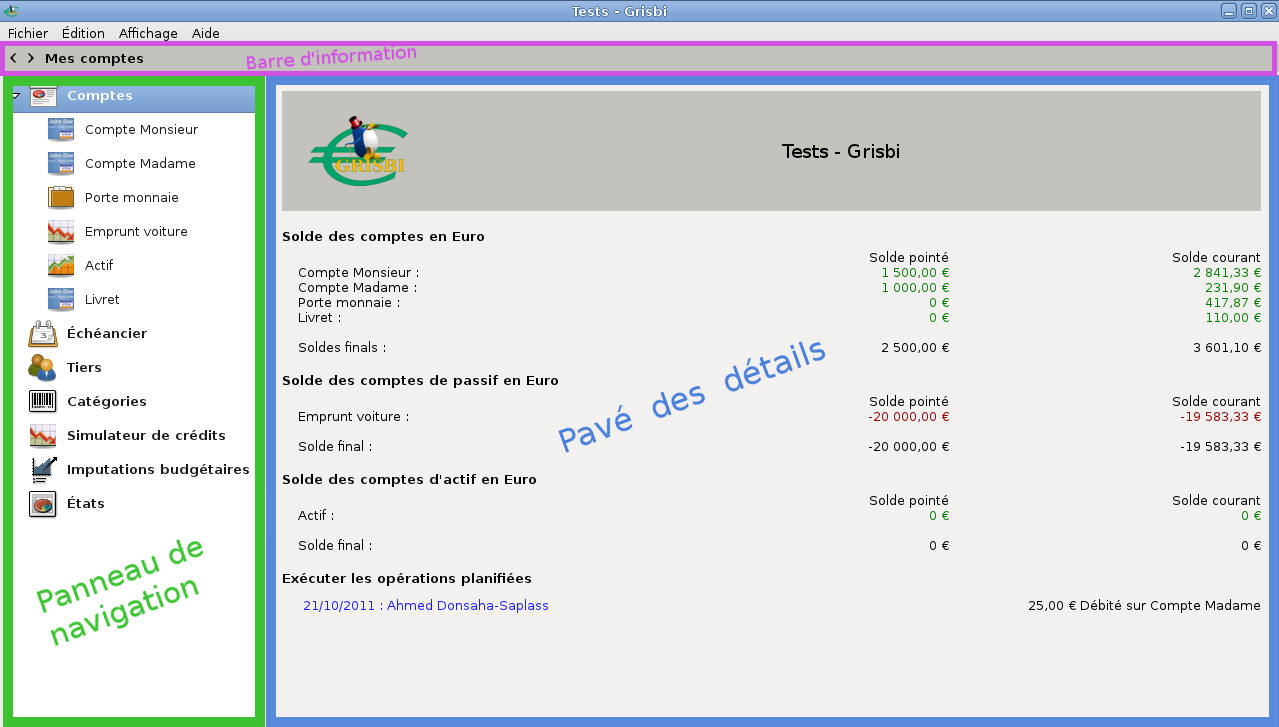
\includegraphics[scale=0.35]{image/screenshot/home}
\end{center}
\caption{Page d'accueil}
\label{home-img}
\end{figure}
% image centrée
\fi

Grisbi affiche toutes ses pages de la même manière : comme n'importe quel logiciel, il affiche une barre de menus qui donne accès à la plupart des fonctionnalités importantes de Grisbi, et aussi trois zones :

\begin{itemize}
	 \item la barre d'information, sous la barre de menus ;
	 \item le panneau de navigation ;
	 \item le pavé des détails.
\end{itemize}

\ifIllustration 
Ces trois zones, spécifiques à Grisbi, sont encadrées de couleurs dans la figure pour bien les identifier\refimage{home-img}.
\else
\fi


\section{Barre d'information\label{home-synthesis}}


La barre d'information affiche le nom de l'onglet courant affiché, et peut afficher, complètement à droite, certains soldes en rapport avec ce qui est sélectionné dans le pavé des détails.

% espace pour changement de thème
\vspacepdf{5mm}
Elle permet, en cliquant successivement sur l'un des deux petits triangles à sa gauche, de sélectionner l'un des onglets affichés dans le panneau de navigation  : \menu{Comptes}, \menu{Échéancier}, \menu{Tiers}, \menu{Simulateur de crédits}, \menu{Catégories}, \menu{Imputations budgétaires} et \menu{États}, et aussi l'un des sous-onglets des onglets \menu{Comptes} et \menu{États} s'ils sont déroulés dans le panneau de navigation.

% Pas de commande au clavier pour cette fonction
\textbf{Note} : ces triangles peuvent être remplacés, en fonction du thème de l'environnement de bureau ou du gestionnaire de fenêtres que vous utilisez, par d'autres caractères tels que +, -, >, <, etc.

% espace pour changement de thème
\vspacepdf{5mm}
Le contenu de la sélection s'affiche dans le pavé des détails.

% espace pour changement de thème
\vspacepdf{5mm}
Ces fonctionnalités peuvent être utilisées à la place de celles du panneau de navigation lorsque sa largeur est réduite à zéro et que l'on n'y a pas accès directement.


\section{Panneau de navigation\label{home-accounting}}


Le panneau de navigation affiche en caractères gras la liste des onglets : \menu{Comptes}, \menu{Échéancier}, \menu{Tiers}, \menu{Simulateur de crédits}, \menu{Catégories}, \menu{Imputations budgétaires} et \menu{États}. En cliquant sur le petit triangle noir à gauche des onglets \menu{Comptes} ou \menu{États}, on peut dérouler ou enrouler la liste de leurs sous-onglets. Vous pouvez changer l'ordre des onglets et des sous-onglets en cliquant sur l'un d'eux et en le déplaçant plus haut ou plus bas dans la liste.

\textbf{Note} : ces triangles peuvent être remplacés, en fonction du thème de l'environnement de bureau ou du gestionnaire de fenêtres que vous utilisez, par d'autres caractères tels que +, -, >, <, etc.

% espace pour changement de thème
\vspacepdf{5mm}
Vous pouvez sélectionner un de ces onglets ou sous-onglets en cliquant sur son nom. Vous pouvez aussi déplacer la sélection dans cette liste d'onglets et de sous-onglets avec les touches du clavier \key{Flèche Haut}, \key{Flèche Bas}, \key{Page Haut} ou \key{Page Bas}, ou avec la molette de la souris. 

% espace pour changement de thème
\vspacepdf{5mm}
Le contenu de la sélection s'affiche dans le pavé des détails. 

% espace pour changement de thème
\vspacepdf{5mm}
On peut réduire ou agrandir la largeur du panneau de navigation en cliquant sur la fine barre verticale entre ce panneau et le pavé des détails, et en la déplaçant. Si la largeur du panneau a été réduite à zéro, ou agrandie au maximum de la largeur de la fenêtre de Grisbi, il faut retrouver cette barre, respectivement complètement à gauche ou à droite de la fenêtre, et la faire glisser à la place désirée. 

% espace pour changement de thème
\vspacepdf{5mm}
Des \indexword{menus contextuels}\index{menu contextuel}, accessibles par un clic-droit de souris, sont disponibles sur les éléments de ce panneau et proposent les fonctions suivantes :

\begin{itemize}
	 \item sur \menu{Comptes} :
		\begin{itemize}
			 \item \menu{Nouveau compte} ;
		\end{itemize}
	 \item sur un compte quelconque : 
		\begin{itemize}
			 \item \menu{Nouveau compte},
			 \item \menu{Supprimer ce compte} ;
		\end{itemize}
	 \item sur \menu{Tiers} :
		\begin{itemize}
			 \item \menu{Nouveau tiers},
			 \item \menu{Supprimer le tiers sélectionné},
			 \item \menu{Éditer le tiers sélectionné},
			 \item \menu{Gérer les tiers},
			 \item \menu{Supprimer les tiers inutilisés} ;
		\end{itemize}
	 \item sur \menu{Catégories} : 
		\begin{itemize}
			 \item \menu{Nouvelle catégorie},
			 \item \menu{Supprimer la catégorie sélectionnée},
			 \item \menu{Editer la catégorie sélectionnée},
			 \item \menu{Importer un fichier de catégories (.csgb)},
			 \item \menu{Exporter la liste des catégories (.csgb)} ;
		\end{itemize}
	 \item sur \menu{Imputations budgétaires} :
		\begin{itemize}
			 \item \menu{Nouvelle imputation budgétaire},
			 \item \menu{Supprimer l'imputation sélectionnée},
			 \item \menu{Editer l'imputation sélectionnée},
			 \item \menu{Importer un fichier d'imputations budgétaires (.isgb)},
			 \item \menu{Exporter la liste des imputations budgétaires (.isgb)} ;
		\end{itemize}
	 \item sur \menu{État} : \menu{Nouvel état} ;
	 \item sur un état quelconque : 
		\begin{itemize}
			 \item \menu{Nouvel état},
			 \item \menu{Supprimer cet état}.
		\end{itemize}
\end{itemize}

\ifIllustration
\else
% saut de page pour titre solidaire
\newpage
\fi


\section{Pavé des détails\label{home-details}}


Le pavé des détails affiche tous les détails sur les onglets ou sous-onglets sélectionnés par la barre d'information ou le panneau de navigation. C'est la zone de travail principale de Grisbi.

On peut réduire ou agrandir sa largeur en cliquant sur la fine barre verticale entre ce pavé et le panneau de navigation, et en la déplaçant. Si la largeur du pavé a été réduite à zéro ou agrandie au maximum de la largeur de la fenêtre de Grisbi, il faut retrouver cette barre, respectivement complètement à droite ou à gauche de la fenêtre, et la faire glisser à la place désirée. 
 
 
\subsection{Affichage de la page d'accueil\label{home-details-homepage}}

Pour afficher la page d'accueil, sélectionnez l'onglet \menu{Comptes} ; le pavé des détails affiche, de haut en bas :

\begin{itemize}
	 \item dans un pavé sur fond gris, l'icône \menu{Grisbi} à gauche, et à droite un \indexword{titre}\index{affichage !titre}\index{titre !page d'accueil} qui permet d'identifier sur quelle comptabilité vous travaillez actuellement, sous la forme \og libellé - Grisbi\fg{} ; vous pouvez définir ce libellé, parmi trois possibilités, dans le menu \menu{Édition - Préférences} (voir le paragraphe \vref{setup-display-addresses-titles}, \menu{Titres}) :
		\begin{itemize}
			 \item l'\menu{Entité comptable} : c'est le nom du domaine de comptabilité sur lequel vous travaillez, par exemple \og Ma comptabilité \fg{} ou \og Association \fg{}, et que vous avez saisi à la création du fichier de comptes ; vous pouvez le modifier ici dans le champ \menu{Nom de l'entité comptable} ; cela peut être utile si vous gérez plusieurs \indexword{entités comptables}\index{entité comptable}, 
			 \item le \menu{Titulaire du compte} : c'est le nom du titulaire (ou du propriétaire) du dernier compte consulté ; si le titulaire n'est pas renseigné dans les propriétés du compte, Grisbi affiche le nom de ce compte,
			 \item le \menu{Nom du fichier de comptes} : c'est le nom du fichier dans le répertoire courant, sous la forme \file{nom\_de\_\_votre\_fichier.gsb}, et c'est le choix par défaut ;
		\end{itemize}
	 \item pour chaque devise séparément, pour tous les comptes et \indexword{groupes de comptes}\index{groupe de comptes}, sous les libellés \menu{Solde rapproché} et \menu{Solde courant} :
		\begin{itemize}
			 \item le solde des comptes bancaires et comptes de caisse, le solde partiel des groupes de comptes et leur solde final,
% saut de ligne pour indentation correcte de la note dans la liste

			 \textbf{Note} : vous pouvez ajuster l'ordre d'affichage des soldes partiels des groupes de comptes (voir le paragraphe \vref{setup-general-home-partBalance}, \menu{Soldes partiels de la liste des comptes}).			 
			 \item le solde des comptes de passif et leur solde final,
			 \item le solde des comptes d'actif et leur solde final ;
		\end{itemize}
	\item les \indexword{alertes des opérations planifiées}\index{alerte !opération planifiée} à échéance ou clôturées, avec leurs date, libellé et montant, selon les choix faits dans le menu \menu{Édition - Préférences} (voir la section \vref{setup-general-planned}, \menu{Échéancier}) ;
	\item la liste des comptes dont le solde est passé sous le \menu{Solde minimal autorisé} ;
	\item la liste des comptes dont le solde est passé sous le \menu{Solde minimal voulu}.
\end{itemize}

% espace avant Attention ou Note  : 5 mm
\vspacepdf{5mm}

\textbf{Note} : pour les définitions du \menu{Solde minimal autorisé} et du \menu{Solde minimal voulu}, voir la section \vref{accounts-properties}, \menu{Propriétés d'un compte}.

% espace pour changement de thème
\vspacepdf{5mm}
Les libellés des comptes s'affichent en noir{\couleur} ; au passage du pointeur de la souris sur la ligne de l'un d'eux, cette couleur passe au gris{\couleur}.
Un solde supérieur au \menu{Solde minimal voulu} s'affiche en vert foncé{\couleur} ; au passage du pointeur sur sa ligne, cette couleur passe au vert clair{\couleur}.
Un solde inférieur au \menu{Solde minimal voulu} et supérieur au \menu{Solde minimal autorisé} s'affiche en orange{\couleur} ; au passage du pointeur sur sa ligne, cette couleur passe à l'orange clair{\couleur}.
Un solde inférieur au \menu{Solde minimal autorisé} s'affiche en rouge{\couleur} ; au passage du pointeur sur sa ligne, cette couleur passe au rouge clair{\couleur}.

Au passage du pointeur de la souris sur la ligne d'un compte, tout changement de couleur indique que si l'on clique (droit ou gauche) avec la souris, ce compte s'affiche, comme s'il avait été sélectionné avec la barre d'information ou le panneau de navigation ; il affiche alors la page qui contient la ligne d'opération  affichant ce solde.

Un solde partiel, qui correspond à un groupe de comptes, s'affiche en noir{\couleur}. S'il est négatif, il peut s'afficher en rouge foncé{\couleur}, mais seulement si cela a été configuré ainsi (voir le paragraphe \vref{setup-general-home-partBalance}, \menu{Soldes partiels de la liste des comptes}). Une ligne de solde partiel ne change pas de couleur au passage du pointeur de la souris dessus, car on ne peut pas afficher les opérations d'un groupe de comptes.

% espace pour changement de thème
\vspacepdf{5mm}
Vous pouvez configurer certains aspects de l'affichage de cette page d'accueil dans le menu \menu{Édition - Préférences} ou dans l'onglet \menu{Propriétés} de chaque compte :
\begin{itemize}
	 \item \menu{\indexword{Polices}\index{polices}, \indexword{logo}\index{logo} et \indexword{couleurs}\index{couleurs}} : section \vref{setup-display-logo} ;
	 \item \menu{Titres} : section \vref{setup-display-addresses-titles} ;
	 \item \menu{Calcul des soldes} : paragraphe \vref{setup-general-home-balance} ;
	 \item \menu{Soldes partiels de la liste des comptes} : paragraphe \vref{setup-general-home-partBalance} ;
	 \item \menu{Alertes de l'échéancier} : section \vref{setup-general-planned} ;
	 \item comptes sous le \menu{\indexword{Solde minimal autorisé}}\index{solde !minimal autorisé} : section \vref{accounts-properties} ;
	 \item comptes sous le \menu{\indexword{Solde minimal voulu}}\index{solde !minimal voulu} : section  \vref{accounts-properties}.
\end{itemize}

En particulier, si vous trouvez une erreur d’orthographe dans cette page, vous pourrez la corriger : voir le paragraphe \vref{setup-general-home-final}, \menu{Pluriel de final} !

\ifIllustration
% saut de page pour paragraphe solidaire
\newpage
\fi

\section{Barre de menus\label{home-menus}}


Comme dans de nombreuses applications graphiques, la plupart des fonctionnalités importantes de Grisbi sont accessibles au moyen des menus de la \indexword{barre de menus}\index{barre de menus}. Nous détaillons ici leurs fonctionnalités.


\subsection{Menu \menu{Fichier}\label{home-menus-file}}

Ce menu comprend les fonctions suivantes :

\begin{itemize}
	\item \menu{Nouveau fichier de comptes} : crée un nouveau fichier de comptes ; le fichier courant est donc fermé et un nouveau fichier vide est créé avec un compte vide (raccourci-clavier \key{Ctrl}\key{N}), voir la section \vref{start-newfile} ; à ne pas confondre avec la création d'un nouveau compte ;
	\item \menu{Ouvrir} : ouvre un fichier de comptes (raccourci-clavier \key{Ctrl}\key{O}) ;
	\item \menu{Derniers fichiers} : affiche la liste des n derniers fichiers ouverts avec Grisbi (seulement s'il y en a eu plusieurs) ; ce nombre est configurable dans le menu \menu{Edition - Préférences}, voir la section \vref{setup-general-files-manage}, \menu{Gestion des fichiers de compte} ;
	\item \menu{Enregistrer} : enregistre le fichier de comptes en cours (raccourci-clavier \key{Ctrl}\key{S}) ;
	\item \menu{Enregistrer sous} : ouvre un gestionnaire de fichiers pour enregistrer le fichier de comptes en cours avec le nom et à l'emplacement de 	votre choix ; Grisbi vous propose par défaut le répertoire courant, le nom du fichier de comptes en cours, avec l'extension \file{.gsb} ;
	\item \menu{Importer un fichier} : démarre l'assistant d'importation de fichiers d'un autre logiciel ; voir la section \vref{move-import-importinit} ;
	\item \menu{Exporter vers un fichier QIF/CSV} : démarre l'assistant d'exportation de fichiers de compte ; voir la section \vref{move-export} ;	
	\item \menu{Créer une archive} : démarre l'assistant de création d'archive ; voir la section \vref{datamanagement-history-new} ;	
	\item \menu{Exporter une archive vers un fichier GSB/QIF/CSV} : démarre l'assistant d'exportation d'archive ; voir la section \vref{datamanagement-history-export} ;
	\item \menu{Déboguer le fichier de compte} : démarre l'assistant de 	débogage de ce fichier, qui va vous aider à chercher des incohérences dans votre fichier de comptes ; voir la section \vref{maintenance-file-debug} ;
	\item \menu{Rendre anonyme le fichier de comptes} : démarre l'assistant qui produit une copie anonymée de votre fichier de comptes ; ce fichier pourra être joint à un rapport de bogue ; voir la section \vref{maintenance-file-anonymous} ;	
	\item \menu{Rendre anonyme le fichier QIF} : démarre l'assistant qui produit une copie anonymée de ce fichier ; ce fichier pourra être joint à un rapport de bogue ; voir la section \vref{maintenance-QIF-anonymous} ;	
	\item \menu{Mode de débogage} : met Grisbi en mode de débogage, qui crée un fichier-journal des évènements ; voir la section \vref{maintenance-debug-mode} ; 	
	\item \menu{Fermer} : ferme le fichier de comptes en cours ; Grisbi vous propose de l'enregistrer si ce n'est déjà fait (raccourci-clavier \key{Ctrl}\key{W}) ;
	\item \menu{Quitter} : ferme Grisbi ; Grisbi vous propose auparavant d'enregistrer le fichier de comptes, si ce n'est pas déjà fait (raccourci-clavier \key{Ctrl}\key{Q}).
\end{itemize}


\subsection{Menu \menu{Édition}\label{home-menus-edit}}

Ce menu comprend les fonctions suivantes :

\begin{itemize}
	\item \menu{Editer l'opération} : voir la section \vref{transactions-modify}, \menu{Modification d'une opération} ;
	\item \menu{Nouvelle opération} : voir la section \vref{transactions-new}, \menu{Saisie d'une nouvelle opération} ;
	\item \menu{Supprimer une opération} : voir la section \vref{transactions-delete}, \menu{Suppression d'une opération} ;
	\item \menu{Utiliser l'opération sélectionnée comme modèle} : voir la section \vref{transactions-model}, \menu{Opération sélectionnée comme modèle} ;
	\item \menu{Cloner l'opération} : voir la section \vref{transactions-duplicate}, \menu{Clonage d'une opération} ;
	\item \menu{Convertir en opération planifiée} : voir la section \vref{transactions-schedule}, \menu{Conversion d'une opération en opération planifiée} ;
	\item \menu{Déplacer l'opération vers un autre compte} : voir la section \vref{transactions-move}, \menu{Déplacement d'une opération vers un autre compte} ;
	\item \menu{Nouveau compte} : voir la section \vref{accounts-new}, \menu{Création d'un nouveau compte} ;
	\item \menu{Supprimer le compte courant} : voir la section \vref{accounts-delete}, \menu{Suppression d'un compte} ;
	\item \menu{Préférences} : permet de configurer Grisbi ; voir le chapitre \vref{setup}, \menu{Configuration de Grisbi}.
\end{itemize}


\subsection{Menu \menu{Affichage}\label{home-menus-display}}

Ce menu comprend les fonctions suivantes : 

\begin{itemize}
	 \item \menu{Montrer le formulaire de saisie d'opérations} ; 
	 \item \menu{Montrer les opérations rapprochées} (raccourci-clavier \key{Alt}\key{R}) ;
	 \item \menu{Montrer les lignes d'archives} (raccourci-clavier \key{Altl}\key{L}) ;
	 \item \menu{Montrer les \indexword{comptes clos}}\index{compte !clos} ;
	 \item \menu{Montrer une ligne par opération} ;
	 \item \menu{Montrer deux lignes par opération} ;
	 \item \menu{Montrer trois lignes par opération} ;
	 \item \menu{Montrer quatre lignes par opération} ;
	 \item \menu{Réinitialiser la largeur des colonnes} ; permet de remettre les colonnes des listes d'opérations à leur largeur d'origine.
\end{itemize}


\subsection{Menu \menu{Aide}\label{home-menus-help}}

La plupart des choix de ce menu donnent accès à des sites Web. Pour que ces accès fonctionnent, il faut avoir indiqué à Grisbi le logiciel de navigation (ou navigateur) que vous souhaitez utiliser, dans le menu \menu{Édition - Préférences} (voir la section \vref{setup-general-programs}, \menu{Programmes}). Le menu \menu{Aide} comprend les choix suivants :

\begin{itemize}
	\item \menu{Manuel} : ouvre votre navigateur à la page \og Manuel de l'Utilisateur de Grisbi \fg{} (raccourci-clavier \key{Ctrl}\key{H}) ;
	\item \menu{Démarrage rapide} : ouvre votre navigateur à la page \og Démarrage Rapide de Grisbi \fg{} ;
	\item \menu{Traduction} : ouvre votre navigateur à la page \og Traduire Grisbi \fg{}, pour vous inviter à nous aider à l'élargissement de 	l'internationalisation de Grisbi ;
	\item \menu{À propos de Grisbi} : affiche la boîte d'information sur l'application : vous y trouverez des détails sur la version, le lien vers le site de Grisbi, les remerciements (contributeurs au projet) et la licence d'utilisation ;
	\item \menu{Site Web de Grisbi} : ouvre votre navigateur à la page du site de \lang{Grisbi}\footnote{\urlGrisbi{}} ;
	\item \menu{Signaler une anomalie} : ouvre votre navigateur à la page du \lang{traqueur de bogues de Grisbi}\footnote{\urlBugTracker{}} pour vous permettre de signaler un bogue que vous auriez découvert. Vous pouvez également suivre sur cette page l'évolution des corrections apportées aux bogues signalés ;
	\item \menu{Astuce du jour} : ouvre une boîte de dialogue qui affiche une astuce d'utilisation, différente à chaque démarrage de Grisbi ; vous pouvez y 	afficher successivement toutes les astuces, et choisir ou non l'affichage de 	l'astuce du jour au démarrage de Grisbi. Pour supprimer ou réactiver l'astuce du 	jour, voir le paragraphe \vref{setup-display-messages-trick}, \menu{Astuce du jour}.
\end{itemize}


\section{Raccourcis-clavier\label{home-shortcuts}}


Les raccourcis-clavier facilitent la saisie des données et la navigation dans les fenêtres de Grisbi, en évitant le recours systématique au déplacement et au clic de la souris. En utilisant ceux correspondant aux manipulations les plus courantes pour vous, vous améliorez votre \indexword{ergonomie}\index{ergonomie} en limitant les mouvements importants de vos bras.
 
Grisbi dispose d'un certain nombre de raccourcis-clavier, présentés ici selon différents thèmes (voir aussi la section \vref{introduction-manual-conventions}, \menu{Conventions typographiques du présent manuel}).


\subsection{Application et fichiers}

\begin{itemize}
	\item Nouveau fichier de comptes : \key{Ctrl}\key{N}
	\item Ouvrir un fichier de comptes : \key{Ctrl}\key{O}
	\item Enregistrer le fichier de comptes : \key{Ctrl}\key{S}
	\item Fermer le fichier de comptes : \key{Ctrl}\key{W}
	\item Fermer Grisbi : \key{Ctrl}\key{Q}
\end{itemize}


\subsection{Panneau de navigation}

\begin{itemize}
	\item Sélectionner un onglet ou un compte : \key{Flèche Haut}, \key{Flèche Bas}, \key{Page Haut} ou \key{Page Bas}
\end{itemize}


\subsection{Liste des opérations et des opérations planifiées}

\begin{itemize}
	\item Sélectionner une opération : \key{Entrée}
	\item Déplacer la sélection : \key{Flèche Haut} ou \key{Flèche Bas}
	\item Nouvelle opération : \key{Entrée} sur ligne vide, ou \key{Ctrl}\key{T}
	\item Modifier une opération : \key{Entrée}
	\item Supprimer une opération : \key{Suppr} ;
	\item Pointer ou dépointer une opération : \key{Ctrl}\key{P}
	\item Rapprocher ou dérapprocher une opération : \key{Ctrl}\key{R}
	\item Montrer ou masquer les opérations rapprochées :  \key{Alt}\key{R}
	\item Montrer ou masquer les lignes d'archives : \key{Altl}\key{L}
\end{itemize}


\subsection{Formulaire de saisie }

\begin{itemize}
	\item La touche \key{Entrée} est configurable : elle permet soit de se déplacer dans le formulaire de saisie, soit de valider l'entrée
	\item Se déplacer au champ suivant : \key{Tabulation} (selon votre choix de configuration)
	\item Annuler la saisie en cours : \key{Échap}
	\item Accepter l'auto-complètement : \key{Tabulation} ou \key{Entrée} (selon votre choix de configuration)
	\item  Symbole de l'euro : \key{AltGr}\key{e}
\end{itemize}


\subsection{Listes déroulantes}

\begin{itemize}
	 \item Ouvrir une liste : \key{Page Bas} ou \key{Flèche bas}
	 \item Se déplacer dans la liste : \key{Flèche haut}, \key{Flèche bas}, \key{Page Haut} ou \key{Page Bas}
	 \item Valider un choix à l'intérieur d'une liste : \key{Entrée}
	 \item Devises, exercices et modes de règlement :
		\begin{itemize}
			\item ouvrir la liste : \key{Espace} ; 
			\item se déplacer dans la liste : \key{Flèche Haut} ou \key{Flèche Bas} ;
			\item valider l'item de la liste : \key{Espace}.
		\end{itemize}
\end{itemize}


\subsection{Dates saisies au calendrier}

\begin{itemize}
	\item Ouvre un calendrier (sur le champ de date) : \key{Ctrl}\key{Entrée}
	\item Ferme le calendrier sans modifier la date : \key{Échap}
	\item Valide la date sélectionnée : \key{Entrée}
	\item Jour suivant ou précédent : \key{+} ou \key{-}, \key{Flèche Droite} ou \key{Flèche Gauche}
	\item Semaine précédente ou suivante : \key{Flèche Haut} ou \key{Flèche Bas}
	\item Mois précédent ou suivant : \key{Page Haut} ou \key{Page Bas}
	\item Premier jour ou dernier jour du mois : \key{Début} ou \key{Fin}
\end{itemize}


\subsection{Dates saisies au clavier}

\begin{itemize}
	\item Jour suivant ou précédent : \key{+} ou \key{-}
	\item Semaine précédente ou suivante : \key{Majuscule} \key{+} ou \key{Majuscule} \key{-}
	\item Mois précédent ou suivant : \key{Page Haut} ou \key{Page Bas}
	\item Année précédente ou suivante : \key{Majuscule} \key{Page Haut} ou \key{Majuscule} \key{Page Bas}
	\item Valide la date sélectionnée \key{Entrée}
\end{itemize}


\subsection{Tiers, catégories, imputations budgétaires, simulateur de crédits, données historiques et prévisions}

\begin{itemize}
	\item Déplacer la sélection : \key{Flèche Haut}, \key{Flèche Bas}, \key{Page Haut} ou \key{Page Bas}
%Ces raccourcis ne fonctionnent plus :
%	\item afficher les sous-catégories ou sous-imputations budgétaires (sur une catégorie ou une imputation budgétaire) : \key{Espace} ;
%	\item afficher les opérations des sous-catégories ou sous-imputations budgétaires (sur une sous-catégorie ou une sous-imputation budgétaire) : \key{Espace}.
\end{itemize}


\subsection{États et Configuration}

\begin{itemize}
	\item Sélectionner un autre onglet : \key{Flèche Haut}, \key{Flèche Bas}, \key{Page Haut}, \key{Page Bas}
	\item Naviguer entre le panneau des onglets et les différentes options du panneau des réglages : \key{Tabulation}, \key{Flèche Haut}, \key{Flèche Bas}, \key{Flèche Gauche} et \key{Flèche Droit}
\end{itemize}

\subsection{Aide}

\begin{itemize}
	\item Ouvre votre navigateur à la page du Manuel de l'Utilisateur de Grisbi \key{Ctrl}\key{H}
\end{itemize}














\myclearemptydoublepage

%%%%%%%%%%%%%%%%%%%%%%%%%%%%%%%%%%%%%%%%%%%%%%%%%%%%%%%%%%%%%%%%%
% Contents: The QIF chapter
% $Id: grisbi-manuel-QIF.tex, v 0.4 2002/10/27 Daniel Cartron
% $Id: grisbi-manuel-QIF.tex, v 0.5.0 2004/06/01 Loic Breilloux
% $Id: grisbi-manuel-QIF.tex, v 0.6.0 2011/11/17 Jean-Luc Duflot
% $Id: grisbi-manuel-QIF.tex, v 0.8.9 2012/04/27 Jean-Luc Duflot
% $Id: grisbi-manuel-QIF.tex, v 1.0 2014/02/12 Jean-Luc Duflot
%%%%%%%%%%%%%%%%%%%%%%%%%%%%%%%%%%%%%%%%%%%%%%%%%%%%%%%%%%%%%%%%%


\chapter{Export et import de comptes\label{move}}

Vous ne pouvez pas utiliser directement dans Grisbi des données qui ont été créées par d'autres applications de comptabilité personnelle, et réciproquement. Comme ces applications fonctionnent différemment, leurs données sont structurées différemment: il faut donc convertir leur structure de données avant de pouvoir les utiliser. 

Cette conversion ne peut pas se faire d'un seul coup sur l'ensemble des données, mais doit se faire indépendamment pour chaque compte géré par l'application. Pour convertir chacun de ces comptes, il faut donc d'une part les \og exporter \fg{} de l'application d'origine, puis les \og importer \fg{} dans l'application de destination.

% espace avant Attention ou Note  : 5 mm
\vspacepdf{5mm}

\strong{Attention} : ne pas confondre LE \og fichier de comptes \fg{} qui contient toutes les données de tous les comptes créés pour la gestion d'une entité comptable (dans Grisbi, ce fichier porte l'\gls{extension} \file{.gsb}), et LES \og fichiers de compte \fg{}, qui sont des fichiers ne contenant que les données d'un seul compte à la fois, et créés uniquement pour exporter ou importer ces données d'une application de comptabilité à une autre. Ces \og fichiers de compte \fg{} doivent avoir un \gls{format de fichier} (ou une extension) obligatoirement compatible avec l'application d'origine ET l'application de destination.
% espace après Attention ou Note  : 5 mm
\vspacepdf{5mm}

Grisbi supporte actuellement les formats de données de compte de comptabilité personnelle \gls{Gnucash}, \gls{OFX}, \gls{CSV} et \gls{QIF}.


\section{Import de comptes d'un autre logiciel\label{move-import}}


Si vous voulez utiliser dans Grisbi des données de comptes qui ont été créés
dans une autre application de comptabilité, vous devez d'abord exporter individuellement chacun des comptes de cette application dans un fichier, puis les importer dans Grisbi grâce à ces fichiers.


\subsection{Export d'un fichier de compte d'un autre logiciel\label{move-import-exportinit}}

La première étape consiste, dans l'application de comptabilité personnelle
d'origine, à exporter chaque compte dans un fichier au format choisi. Le format choisi doit être compatible à l'exportation par l'application d'origine \emph{et} compatible à l'importation par Grisbi.

La procédure d'exportation est bien évidemment différente pour chaque logiciel, donc référez-vous à sa documentation. Si vous voulez exporter tous les comptes, vous devrez obtenir autant de fichiers que vous avez de comptes gérés par l'application.


\subsection{Import de fichiers de compte d'un autre logiciel dans Grisbi\label{move-import-importinit}}

\textbf{Note} : Grisbi permet d'importer un ou plusieurs fichiers de compte au cours de la même procédure. Bien que l'on puisse importer les fichiers de compte un par un, il est important de bien importer tous les fichiers de compte simultanément, afin que Grisbi puisse recréer les liens entre les comptes, particulièrement en ce qui concerne les opérations de virement.
% espace après Attention ou Note  : 5 mm
\vspacepdf{5mm}

Pour plus de renseignements sur les \indexword{types de compte}\index{types de compte} que Grisbi sait gérer,  voir la section \vref{accounts-type}, \menu{Types de comptes de Grisbi}.

Vous pouvez définir quelle date sera utilisée pour l'attribution d'un exercice à 
chaque opération importée, voir le paragraphe \vref{setup-general-import-financialyear}, \menu{Définition de l'exercice}.

Lorsque vous importez un fichier, Grisbi vous permet d'établir une association entre une chaîne de caractères de ce fichier et un tiers. Par exemple, tous les libellés contenant \og loyer \fg{} peuvent être associés à un tiers qui représente votre propriétaire. Cela doit être configuré dans le menu \menu{Édition - Préférences} (voir la section \vref{setup-general-importLinks}, \menu{Associations pour l'import}).

% espace pour changement de thème
\vspacepdf{5mm}
Dans le menu \menu{Fichier} de Grisbi, choisissez l'option \menu{Importer un
fichier}, ce qui ouvre la fenêtre de l'assistant d'importation. L'importation des fichiers de compte se déroule en cinq étapes :

\begin{enumerate}
	\item accueil de l'assistant d'importation ; validez par le bouton \menu{Suivant} ;
	\item sélection des fichiers de compte à importer :	
		\begin{enumerate}
			\item cliquez sur le bouton \menu{Ajouter un ou des fichiers} : une fenêtre de gestionnaire de fichiers s'ouvre,	
			\item cherchez le répertoire où se trouvent ces fichiers de compte,
			\item sélectionnez un ou plusieurs fichiers de compte (avec la combinaison  \key{Ctrl}\key{Clic} et \key{Majuscule}\key{Clic}) ; vous pouvez aussi changer la \gls{locale} (\gls{encodage des caracteres}) des fichiers à importer dans le menu déroulant \menu{Codage},
			\item validez la fenêtre pour revenir à la fenêtre de sélection des fichiers de compte,
			\item si les sélections voulues sont bien cochées, vous pouvez valider par le bouton \menu{Suivant} ;
		\end{enumerate}		  
	\item fin de la préparation de l'importation des fichiers de compte : si tout s'est bien passé, cette fenêtre donne la liste des fichiers de compte qui seront importés ; continuez l'importation en validant par le bouton \menu{Suivant} ;
	\item création et paramétrage de chaque compte importé dans Grisbi : vous pouvez passer en revue chaque compte et y choisir les actions suivantes \ifIllustration \refimage{QIF-import-files-setup-img} :
	% image centrée
	\begin{figure}[htbp]
	\begin{center}
	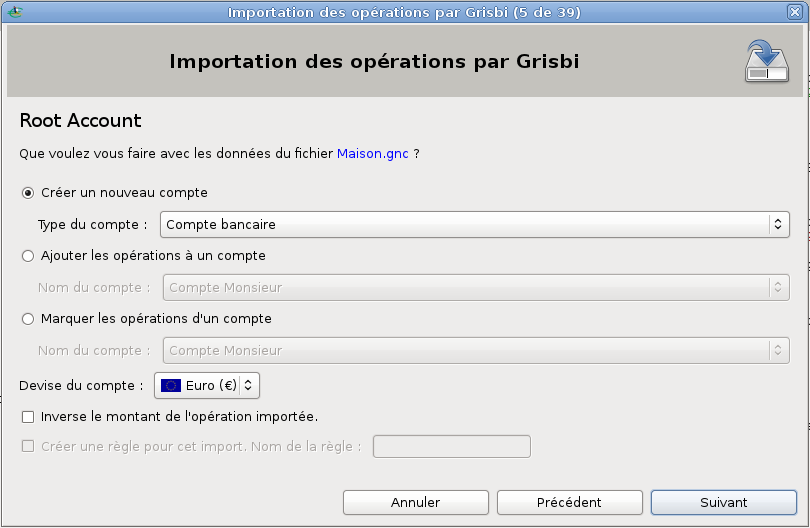
\includegraphics[scale=0.5]{image/screenshot/QIF_import_files_setup}
	\end{center}
	\caption{Paramétrage de chaque compte importé}
	\label{QIF-import-files-setup-img}
	\end{figure}
	% image centrée
	\else  :
	\fi
	
		\begin{itemize}
			\item créer un nouveau compte,
			\item ajouter des opérations à un compte : si des opérations planifiées sont trouvées dans l'intervalle de temps spécifié, une fenêtre spécifique s'ouvre pour savoir ce que vous voulez en faire : soit fusionner ces opérations planifiées avec les opérations importées correspondantes, soit ajouter les opérations importées en sus de celles-là (voir la section \vref{setup-general-import-parameters}, \menu{Paramètres pour l'import}),
			\item marquer les opérations d'un compte : si des \indexword{opérations orphelines}\index{opération !orpheline} sont trouvées, une fenêtre s'ouvrira en fin d'import pour savoir ce que vous voulez en faire : soit les ajouter, soit les ignorer,
			\item définir la devise du compte (ou bien en créer une nouvelle),
			\item   inverser le montant de l'opération (utile pour les comptes de carte bancaire de la Banque Postale, par exemple),
			\item créer une règle d'importation rapide si le fichier est au format QIF ou OFX,
			\item quand tout est correct, validez l'importation par le bouton \menu{Suivant} ;
		\end{itemize}
	
	 \item validation de la fin de l'importation : valider par le bouton \menu{Fermer}.
\end{enumerate}

Si, et seulement si vous venez de créer votre fichier de comptes juste avant cette importation de données de comptes, revenez à la fin de la section \vref{start-newfile-end}, \menu{Création d'un nouveau fichier de comptes}. Allez juste après la fin de la procédure de création du fichier de comptes, au paragraphe commençant par \emph{D'une manière ou d'une autre\ldots{ }}, ce qui vous proposera de créer tout de suite d'autres comptes.

%espace pour changement de thème
\vspacepdf{5mm}
Sinon, vous pouvez commencer à utiliser le compte que vous venez de créer.


\section{Export de comptes à partir de Grisbi\label{move-export}}


Si vous voulez utiliser, dans une autre application de comptabilité, des données de compte qui ont été créées par Grisbi, vous devez d'abord exporter ces données dans des fichiers, puis les importer dans l'autre application grâce à ces fichiers. Le format de fichier choisi doit être compatible à l'exportation par Grisbi \emph{et} compatible à l'importation par l'application de destination.
 
Dans le menu \menu{Fichier} choisissez l'option \menu{Exporter vers un fichier QIF/CSV/\ldots{ }} qui ouvre l'assistant Export des comptes. L'exportation des comptes comporte quatre étapes :

\begin{enumerate}
	\item accueil de l'assistant ; cette fenêtre indique que, comme les formats de fichier QIF et CSV ne supportent pas les devises, toutes les opérations seront converties dans la devise de leur compte respectif ; validez par le bouton \menu{Suivant} ;
	\item sélectionnez les comptes à exporter en cliquant dans la case correspondante ; validez par le bouton \menu{Suivant} ;
	\item pour chaque compte, définissez le nom du fichier, le répertoire de destination et le format d'exportation, puis validez par le bouton \menu{Suivant} \ifIllustration \refimage{QIF-export-img} ;
	% image centrée
	\begin{figure}[t]
	\begin{center}
	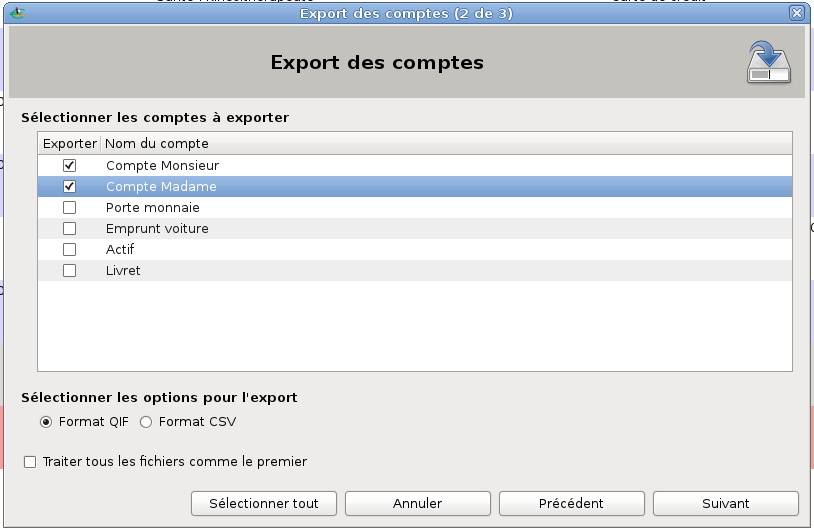
\includegraphics[scale=0.5]{image/screenshot/QIF_export}
	\end{center}
	\caption{Export des comptes}
	\label{QIF-export-img}
	\end{figure}
	% image centrée
	\else  ;
	\fi
	
	\item la fenêtre de fin de l'exportation s'affiche ; validez par le bouton \menu{Fermer}.
\end{enumerate}

\strong{Attention} : d'une manière générale, il est déconseillé d'avoir des accents ou des espaces dans les noms des répertoires et fichiers utilisés par Grisbi. Si c'est le cas, renommez-les maintenant. Par exemple, les espaces peuvent être remplacées par des tirets bas (\_).












\myclearemptydoublepage

%%%%%%%%%%%%%%%%%%%%%%%%%%%%%%%%%%%%%%%%%%%%%%%%%%%%%%%%%%%%%%%
% Contents : The data management chapter
% $Id : grisbi-manuel-datamanagement.tex, v 0.8.9 2012/04/27 Jean-Luc Duflot
% $Id : grisbi-manuel-datamanagement.tex, v 1.0 2014/02/12 Jean-Luc Duflot
%%%%%%%%%%%%%%%%%%%%%%%%%%%%%%%%%%%%%%%%%%%%%%%%%%%%%%%%%%%%%%%%%

\chapter{Gestion des données\label{datamanagement}}


Les données que vous avez entrées dans Grisbi et les traitements que vous en avez faits sont en nombre important ; de ce fait ils ne doivent en aucun cas être perdus, et leur quantité ne doit pas être un obstacle à leur bonne gestion. Grisbi propose donc trois outils pour faire face à ces problématiques : \menu{Gestion des fichiers de comptes}, \menu{Sauvegardes} et \menu{Archives}.


\section{Gestion des fichiers de comptes\label{datamanagement-files}}


Vous pouvez définir les options de gestion suivantes :

\begin{itemize}
	\item le chargement automatique du dernier fichier consulté ;
	\item l'enregistrement automatique lors de la fermeture ;
	\item le \indexword{forçage de l'enregistrement}\index{enregistrement !forçage} des fichiers verrouillés ;
	\item le \indexword{chiffrement du fichier de comptes}\index{fichier de comptes !chiffrement}\index{chiffrement !fichier de comptes} ;
	\item la \indexword{\gls{compression}} du fichier de comptes\index{fichier de comptes !compression}\index{compression !fichier de comptes} ;
	\item la mémorisation des derniers fichiers ouverts.
\end{itemize}

Toutes ces options sont explicitées en détail et peuvent être configurées dans le menu \menu{Édition - Préférences} (voir le paragraphe \vref{setup-general-files-manage}, \menu{Gestion des fichiers de comptes}).


\section{Sauvegardes\label{datamanagement-backup}}


D'une manière générale, quelles que soient les données que vous possédez dans le disque dur de votre ordinateur, vous devez impérativement en faire des sauvegardes, pour la simple raison que \emph{tout système de stockage de données a une durée de vie limitée}. Faire des sauvegardes a pour but de limiter les risques de pertes de données. 

Grisbi vous permet de faire des sauvegardes automatiques de votre fichier de comptes. Ces sauvegardes devraient être stockées dans un répertoire spécial ou une \gls{partition} spéciale du disque de votre ordinateur, avec les sauvegardes de toutes vos autres données, ce qui vous permettrait alors de sauvegarder facilement ce répertoire ou cette partition, de préférence sur des supports de type différents, indépendants de l'ordinateur, et mis en lieu sûr.

% espace avant Attention ou Note  : 5 mm
\vspacepdf{5mm}
\textbf{Note} : vous êtes maintenant prévenu(e), prenez ces conseils au sérieux : ne prenez pas de risques avec vos données, cela peut vous éviter bien des déboires\ldots
% espace après Attention ou Note  : 5 mm
\vspacepdf{5mm}

Grisbi peut enregistrer automatiquement, dans un répertoire à définir, soit un fichier de sauvegarde unique qui est remplacé régulièrement, soit des fichiers de sauvegarde qui s'accumulent dans ce répertoire.

Les fichiers de sauvegarde ont un nom de la forme \file{nom\_du\_fichier\_AAAAMMJJTHHMMSS.gsb}, où \emph{nom\_du\_fichier} est le nom de votre fichier de comptes, \emph{AAAAMMJJ} est la date en année-mois-jours, \emph{T} est un séparateur, et \emph{HHMMSS} est l'heure en heures-minutes-secondes. Ce format est basé sur le format international de date ISO 8601, ce qui permet, entre autres, le classement automatique dans l'ordre alphanumérique et chronologique dans votre répertoire de sauvegarde.

%espace pour changement de thème
\vspacepdf{5mm}
 Grisbi vous propose les options de sauvegarde suivantes :

\begin{itemize}
	\item la création d'un fichier de sauvegarde unique, sinon les fichiers de sauvegarde s'ajoutent dans  leur répertoire ;
	\item la \indexword{\gls{compression} du fichier de sauvegarde}\index{fichier de sauvegarde !compression}\index{compression !fichier de sauvegarde}, pour occuper moins d'espace disque ;
	\item la sauvegarde après l'ouverture du fichier de comptes ; 
	\item la sauvegarde avant l'enregistrement du fichier de comptes ; 
	\item le réglage de l'intervalle entre deux sauvegardes, en minutes ;
	\item la définition du \indexword{répertoire de sauvegarde}\index{répertoire de sauvegarde}\index{fichier de sauvegarde !répertoire}.
\end{itemize}

%espace pour changement de thème
\vspacepdf{5mm}
Toutes ces options sont décrites en détail et peuvent être configurées dans le menu \menu{Édition - Préférences} (voir le paragraphe \vref{setup-general-files-backup}, \menu{Sauvegardes}).


\section{Archives\label{datamanagement-history}}


Une archive est une sorte de \og mise entre parenthèses \fg{} d'une partie des opérations de tous les comptes de votre fichier de comptes. Les opérations à l'intérieur d'une archive ne sont plus affichées et ne peuvent plus faire l'objet de traitements, mais elles sont toujours conservées dans ce fichier. Vous pouvez toujours et à tout moment désarchiver une archive existante pour en afficher les opérations et l'inclure dans un traitement. 

Lorsque vous utilisez Grisbi, vous entrez des opérations dans vos différents comptes. Ces opérations sont toutes enregistrées dans la mémoire et sur le disque dur de l'ordinateur, et une petite partie est affichée sur l'écran. L'affichage et le traitement des opérations consomme donc de la mémoire et du temps de microprocesseur.

Au fur et à mesure que le temps passe, il y a de plus en plus d'opérations enregistrées, donc leur affichage et leurs traitements demandent de plus en plus d'espace mémoire et de temps de microprocesseur. Votre ordinateur devient donc de plus en plus lent, mais évidemment, cela dépend toujours de ses propres caractéristiques.

Pour limiter cette perte de performances dans l'affichage et le traitement, en particulier dans l'établissement d'états ou dans la recherche d'informations, Grisbi vous propose de choisir une partie des opérations et de les mettre dans une archive, c'est-à-dire de les mettre à part pour leur éviter d'être concernées par de futurs affichages ou traitements.  

La mise en archive peut être manuelle ou automatisée. Grisbi considère qu'au-delà de trois mille opérations{\valeur} dans un compte, les traitements deviennent trop lents, donc d'une part il vous avertit si vous dépassez ce nombre d'opérations et vous propose d'en archiver manuellement une partie, d'autre part il peut vous proposer d'archiver ces  trois mille opérations en lançant automatiquement un assistant.

Que vous fassiez un archivage manuellement ou avec l'assistant, le processus de comptage est ensuite remis à zéro et Grisbi vous proposera de nouveau la même chose après trois mille opérations supplémentaires.


\subsection{Archives dans la liste des opérations\label{datamanagement-history-list}}

L'\indexword{affichage d'une archive}\index{archive !affichage} apparaît tout en haut de la liste des opérations \emph{de chaque compte}, sous la forme d'une ligne d'opération sur fond vert{\couleur}, indiquant sa date de création, son nom et ses paramètres de création (dates, exercice ou état), ainsi que \ifIllustration le \indexword{nombre d'opérations archivées}\index{archive !nombre d'opérations} \emph{pour le compte affiché}, et le \indexword{nombre total d'opérations}\index{opération !nombre total} dans votre fichier de comptes\refimage{datamanagement-history-line-img}.

% image centrée
\begin{figure}[htbp]
\begin{center}
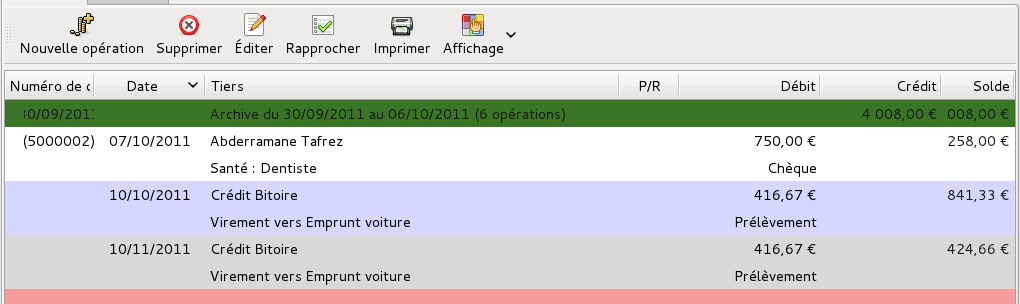
\includegraphics[scale=0.5]{image/screenshot/datamanagement_history_line}
\end{center}
\caption{Ligne d'une archive}
\label{datamanagement-history-line-img}
\end{figure}
% image centrée
\else le \indexword{nombre d'opérations archivées}\index{archive !nombre d'opérations} \emph{pour le compte affiché}, et le \indexword{nombre total d'opérations}\index{opération !nombre total} dans votre fichier de comptes.
\fi

Vous pouvez afficher ou masquer toutes les lignes d'archives dans la liste des opérations de tous les comptes en sélectionnant le menu \menu{Affichage - Montrer les lignes d'archives}, ou en cliquant sur l'outil \menu{Affichage} de la barre d'outils, puis en sélectionnant \menu{Montrer les lignes d'archives} dans sa liste déroulante.

Si vous voulez consulter les opérations à l'intérieur d'une archive, vous pouvez ouvrir cette archive en double-cliquant sur sa ligne : après validation dans la fenêtre qui apparaît, les opérations sont affichées dans la liste. 

\textbf{Note} : il ne s'agit que d'une ouverture de l'archive pour affichage, et en aucun cas cette archive n'est supprimée. À la prochaine utilisation de Grisbi, la ligne verte de l'archive réapparaîtra en haut de la liste de chaque compte. Pour une véritable suppression de l'archive, voir la section \vref{datamanagement-history-remove}, \menu{Suppression d'une archive}.


\subsection{Création d'une archive\label{datamanagement-history-new}}

Pour créer une archive, procédez comme suit :

\begin{enumerate}
	\item dans la barre de menus, sélectionnez \menu{Fichier - Créer une archive} : la fenêtre de l'assistant de création d'archive s'affiche ; validez par le bouton \menu{Suivant} ;
	\item dans la fenêtre suivante, vous pouvez choisir le mode de sélection des opérations à \ifIllustration archiver\refimage{datamanagement-history-create-img} :
	% image centrée
	\begin{figure}[htbp]
	\begin{center}
	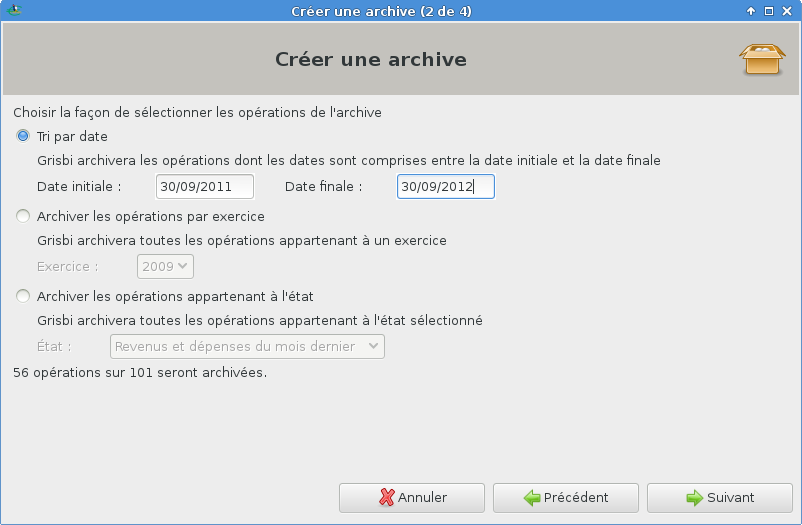
\includegraphics[scale=0.5]{image/screenshot/datamanagement_history_create}
	\end{center}
	\caption{Création d'une archive}
	\label{datamanagement-history-create-img}
	\end{figure}
	% image centrée
	\else archiver :
	\fi
	
		\begin{itemize}
			\item \menu{Tri par date} : saisissez les \menu{Date initiale} et \menu{Date finale} dans les champs adéquats,
			\item \menu{Archiver les opérations par exercice} : sélectionnez un exercice disponible dans la liste déroulante,
			\item \menu{Archiver les opérations appartenant à l'état} : sélectionnez un état disponible dans la liste déroulante ;
% saut de ligne pour indentation correcte de la note dans la liste

			\textbf{Note} : la dernière ligne dans la fenêtre indique soit une erreur de saisie de ces paramètres, soit le nombre d'opérations qui seront archivées et le nombre total d'opérations de votre fichier de comptes.  
		\end{itemize}
	\item validez par le bouton \menu{Suivant} ;
	\item dans la fenêtre suivante, saisissez le nom que vous voulez pour cette archive ; validez par le bouton \menu{Appliquer} ;
	\item la dernière fenêtre vous informe que l'archive a été créée, et affiche le \indexword{nombre d'opérations archivées}\index{archive !nombre d'opérations} et le nombre total d'opérations de votre fichier de comptes, \emph{tous comptes confondus} ; validez par le bouton \menu{Précédent} pour créer une autre archive, sinon par le bouton \menu{Fermer}.
\end{enumerate}

\textbf{Note} :  au cas où Grisbi serait devenu plus lent après avoir créé une archive, vous pouvez le configurer pour ne pas charger les opérations rapprochées (R) au démarrage, afin d'augmenter sa rapidité (voir la section \ref{transactions-functions}, \menu{Barre d'outils}).

% espace après Attention ou Note  : 5 mm
\vspacepdf{5mm}
L'archive apparaît alors tout en haut de la liste des opérations \emph{de chaque compte} (voir la section \vref{datamanagement-history-list}, \menu{Archives dans la liste des opérations}).


\subsection{Avertissement de création et création automatique d'archives\label{datamanagement-history-auto}}

Lorsqu'un certain nombre d'opérations enregistrées est atteint, Grisbi peut d'une part vous avertir que cette quantité d'opérations n'a pas été encore archivée, d'autre part lancer automatiquement la création d'une d'archive  (voir le paragraphe \vref{setup-general-archives-create}, \menu{Avertissement et création automatique}).

En cliquant sur la case libellée \menu{Créer automatiquement une archive si nécessaire}, vous validez la fonction d'archivage automatique.

Avec le libellé \menu{Avertir si plus de \ldots{ } opérations ne sont pas archivées}, vous pouvez définir ce nombre d'opérations. La valeur par défaut est 3000.


\subsection{Paramètres d'une archive\label{datamanagement-history-parameters}}

Vous pouvez consulter les paramètres qui ont été définis pendant la création d'une archive, dans le menu
\menu{Édition - Préférences - Archives}. Pour cela, voir la section \vref{setup-general-archives-existing}, \menu{Archives existantes}.


\subsection{Modification d'une archive\label{datamanagement-history-modify}}

Vous pouvez, uniquement, \indexword{modifier le nom d'une archive}\index{archive !modification} dans le menu \menu{Édition - Préférences}. Pour cela, voir le paragraphe \vref{setup-general-archives-remove}, \menu{Modifier l'archive}.


\subsection{Suppression d'une archive\label{datamanagement-history-remove}}

Vous pouvez \indexword{supprimer une archive}\index{archive !suppression} existante, dans le menu \menu{Édition - Préférences}. Il y a deux fonctions de suppression distinctes : la suppression d'une archive tout en \emph{conservant} ses opérations, et la suppression d'une archive tout en \emph{supprimant} toutes ses opérations. Pour cela, voir le paragraphe \vref{setup-general-archives-remove}, \menu{Modifier l'archive}. 


\subsection{Export d'une archive\label{datamanagement-history-export}}

Exporter une archive permet de créer un fichier contenant l'archive, afin de la stocker, ou de l'utiliser dans un autre fichier de comptes de Grisbi ou dans une autre application de comptabilité. L'exportation ne peut se faire qu'à travers les formats de fichiers \indexword{\gls{GSB}}\index{gsb}, \indexword{\gls{QIF}}\index{qif} ou \indexword{\gls{CSV}}\index{csv}.

% espace avant Attention ou Note  : 5 mm
\vspacepdf{5mm}
\strong{Attention} : les formats de fichiers QIF et CSV ne supportent pas les devises, et toutes les opérations seront converties dans la devise de leur compte respectif.
% espace après Attention ou Note  : 5 mm
\vspacepdf{5mm}

Pour exporter une archive, procédez comme suit :

\begin{enumerate}
	\item dans la barre de menus, sélectionnez \menu{Fichier - Exporter une archive vers un fichier GSB, QIF ou CSV... } : la fenêtre de l'assistant d'exportation d'archive s'affiche ; validez par le bouton \menu{Suivant} ;
	\item un tableau affiche la liste des archives existantes avec leur nom et, selon le cas, leurs dates initiale et finale, leur exercice ou le nom de l'état ; sélectionnez l'archive à exporter en cochant la case dans sa ligne ; validez par le bouton \menu{Suivant} ;
	\item une fenêtre de gestionnaire de fichiers s'affiche ; modifiez éventuellement le nom du fichier sous lequel l'archive sera exportée, le dossier où elle sera enregistrée et le format du fichier d'exportation ; validez par le bouton \menu{Suivant} ;
	\item la dernière fenêtre vous informe que l'archive a été exportée ; validez par le bouton \menu{Fermer}.
\end{enumerate}










\myclearemptydoublepage

%%%%%%%%%%%%%%%%%%%%%%%%%%%%%%%%%%%%%%%%%%%%%%%%%%%%%%%%%%%%%%%%%
% Contents : The accounts chapter
% $Id : grisbi-manuel-accounts.tex, v 0.4 2002/10/27 Daniel Cartron
% $Id : grisbi-manuel-accounts.tex, v 0.5.0 2004/06/01 Loic Breilloux
% some of its content was in tips chapter : 
% $Id : grisbi-manuel-tips.tex, v 0.4 2002/10/27 Daniel Cartron
% $Id : grisbi-manuel-accounts.tex, v 0.6.0 2011/11/17 Jean-Luc Duflot
% some of its content was in tips chapter :
% $Id : grisbi-manuel-tips.tex, v 0.5.0 2004/06/01 Loic Breilloux
% $Id : grisbi-manuel-accounts.tex, v 0.8.9 2012/04/27 Jean-Luc Duflot
% $Id : grisbi-manuel-accounts.tex, v 1.0 2014/02/12 Jean-Luc Duflot
% some of its content was in transactions chapter :
% $Id : grisbi-manuel-transactions.tex, v 0.8.9 2012/04/27 Jean-Luc Duflot
%%%%%%%%%%%%%%%%%%%%%%%%%%%%%%%%%%%%%%%%%%%%%%%%%%%%%%%%%%%%%%%%%

\chapter{Gestion des comptes\label{accounts} }

Grisbi sait gérer quatre types de compte, dont l'utilisation est décrite précisément dans la section \vref{accounts-type}, \menu{Types de compte de Grisbi} :
\begin{itemize}
	\item \indexword{compte bancaire}\index{compte !bancaire} : il permet de faire tout type d'opération ;
	\item \indexword{compte de caisse}\index{compte !caisse} : il ne permet de gérer que des espèces ;
	\item \indexword{compte de passif}\index{compte !passif} : il permet de gérer une dette que vous remboursez ; 
	\item \indexword{compte d'actif}\index{compte !actif} : il permet de gérer un bien qui se déprécie avec le temps. 
\end{itemize}


\section{Liste des comptes\label{accounts-list}}


Pour lister les comptes, déroulez d'abord l'onglet \menu{Comptes} dans le panneau de navigation en cliquant sur le petit triangle à sa gauche. Le panneau de navigation affiche la liste des comptes, que vous pouvez faire défiler en cliquant successivement sur l'un des deux petits triangles à gauche dans la barre d'information.

% espace avant Attention ou Note  : 5 mm
%\vspacepdf{5mm}
\textbf{Note} : ces triangles peuvent être remplacés, en fonction du thème de l'environnement de bureau ou du gestionnaire de fenêtres que vous utilisez, par d'autres caractères tels que +, -, >, <, etc.

% On pourrait dérouler la liste au clavier par la touche Espace, par exemple.

% espace pour changement de thème
\vspacepdf{5mm}
Vous pouvez modifier l'ordre d'affichage des comptes dans le panneau de navigation, en cliquant et déplaçant le nom d'un compte vers le haut ou vers le bas dans la liste des comptes du panneau de navigation.


\section{Sélection d'un compte\label{accounts-selection}}


Pour sélectionner et afficher le contenu d'un compte, utilisez l'une des méthodes suivantes :

\begin{itemize}
	 \item cliquez sur son nom dans le panneau de navigation ;
	 \item déplacez la sélection avec les touches  du clavier \key{Flèche Haut},  \key{Flèche Bas}, \key{Page Haut} ou \key{Page Bas}, ou avec la molette de la souris ;
	 \item dans la barre d'information, cliquez sur l'un des deux petits triangles à gauche pour faire défiler les comptes.
\end{itemize}

\textbf{Note} : ces triangles peuvent être remplacés, en fonction du thème de l'environnement de bureau ou du gestionnaire de fenêtres que vous utilisez, par d'autres caractères tels que +, -, >, <, etc.

% espace pour changement de thème
\vspacepdf{5mm}
Le panneau de navigation affiche le nom du compte sur fond bleu{\couleur} ; la barre d'information affiche, à gauche, le nom du compte sélectionné et, complètement à droite, le solde de ce compte ; le pavé des détails affiche la liste des opérations dans l'onglet \menu{Opérations}.

% espace pour changement de thème
\vspacepdf{5mm}
Le pavé des détails affiche par défaut deux onglets, pour les comptes de banque ou de caisse :
\begin{itemize}
	 \item l'onglet \menu{Opérations} ;
	 \item l'onglet \menu{Propriétés}.
\end{itemize}

Il peut aussi afficher, si le module budgétaire a été activé pour le compte sélectionné, trois autres onglets qui ne sont pas décrits dans ce chapitre (voir le chapitre \vref{budget}, \menu{Budgets Prévisionnels}) :
\begin{itemize}
	 \item soit les onglets \menu{Prévisions} et \menu{Données historiques}, pour les comptes de banque ou de caisse ;
	 \item soit l'onglet \menu{Tableau d'amortissement}, pour les comptes de passif.
\end{itemize}


% espace pour changement de thème
\vspacepdf{5mm}
Il se peut que certains comptes soient \indexword{clos}\index{compte !clos}, donc leur affichage est masqué. Vous pouvez cependant les afficher en sélectionnant le menu \menu{Affichage - Montrer les comptes clos}. Pour faire l'opération inverse, voir la section \vref{accounts-properties}, \menu{Propriétés d'un compte}. 


\section{Propriétés d'un compte\label{accounts-properties}}


L'onglet \menu{Propriétés} permet de renseigner et d'afficher les informations relatives au compte \ifIllustration sélectionné\refimage{account-new-properties-img}.
\else sélectionné.
\fi

\ifIllustration
% image centrée
\begin{figure}[h!]
\begin{center}
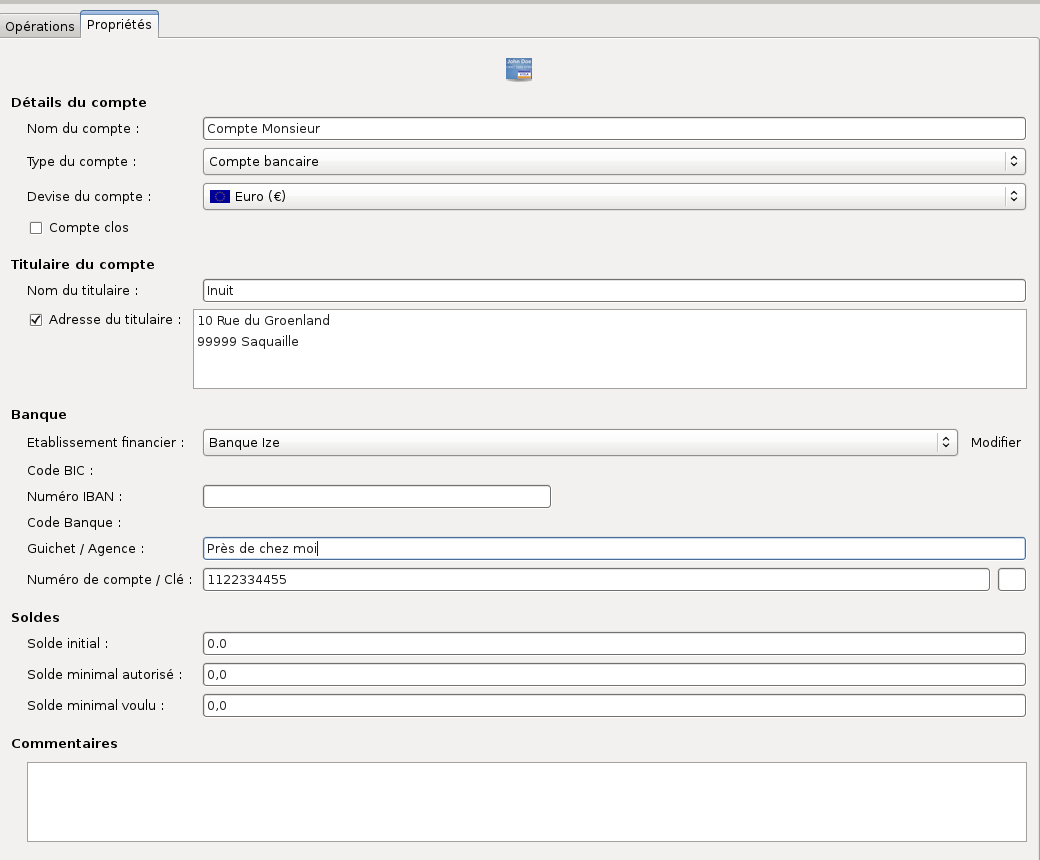
\includegraphics[scale=0.48]{image/screenshot/account_new_properties}
\end{center}
\caption{Propriétés d'un compte}
\label{account-new-properties-img}
\end{figure}
% image centrée
\fi

Pour afficher les propriétés d'un compte, sélectionnez-le, puis cliquez sur l'onglet \menu{Propriétés} dans le pavé des détails. Cet onglet affiche toutes les informations et propriétés qui ont déjà été renseignées sur le compte \ifIllustration sélectionné\refimage{account-new-properties-img}.
\else sélectionné.
\fi
Pour modifier ces données, voir la section \vref{accounts-modify}, \menu{Modifier un compte}.

Voici les différentes informations qu'un compte peut contenir :

\begin{itemize}
	\item \menu{Nom du compte} : ce peut-être un nom quelconque, par exemple \emph{Compte courant}, \emph{Compte livret}, \emph{Compte banque 1} ou \emph{Compte banque 2};	
% saut de ligne pour indentation correcte de la note dans la liste

\textbf{Note} : dans le cas d'une comptabilité numérotée (association ou petite entreprise), les noms des comptes sont précédés du numéro fourni par le plan comptable, par exemple \og 512. Compte banque X \fg{} ; ce libellé est donc une donnée alphanumérique.

	\item \menu{Type du compte} : pour plus de détails, voir la section \vref{accounts-type} ;	
	\item \menu{Devise du compte} : la devise dans laquelle les opérations de ce compte sont libellées (voir les sections \vref{setup-resources-currencies} et \vref{setup-resources-rate}) ;	
	\item \menu{{Compte clos}}\index{compte !clos} : case à cocher qui vous permet de masquer le compte dans le panneau de navigation et dans la barre d'information, sans pour autant le supprimer ; il pourra être affiché à nouveau en cliquant sur le menu \menu{Affichage - Montrer les comptes clos} ;	
	\item \menu{Nom du titulaire} : le titulaire d'un compte peut être différent pour chaque compte, par exemple si vous ouvrez un livret d'épargne pour chacun de vos enfants ;	
	 \item \menu{Adresse du titulaire} : le titulaire peut avoir la même adresse que le titulaire principal, ou bien une adresse différente qu'il faudra préciser ici (voir le paragraphe \vref{setup-display-addresses-address}, \menu{Adresses}) ;
	\item \menu{Établissement financier} : la banque qui gère votre compte ; vous pouvez choisir une banque indiquée dans la liste déroulante, ou bien cliquer sur \menu{Ajouter une nouvelle banque} ; il est conseillé de renseigner ce champ (voir la section \vref{setup-resources-banks}) ;	
	\item \menu{Numéro \gls{IBAN}} : le code que vous trouverez sur votre relevé d'identité bancaire (RIB) ou IBAN fourni par la banque (voir la section \vref{setup-resources-banks}) ;	
	\item \menu{Guichet / Agence} : l'adresse de votre agence bancaire, à relever également sur votre RIB (voir la section \vref{setup-resources-banks}) ;	
	\item \menu{Numéro du compte / Clé} : voir sur votre RIB (voir la section \vref{setup-resources-banks}) ;	
	\item \menu{Solde initial} : le solde de votre dernier relevé bancaire au moment de la création du compte ; il est conseillé de laisser le solde initial du compte à zéro et de créer par la suite une opération initiale du montant nécessaire, car cela facilitera la gestion future des rapprochements ;	
	\item \menu{Solde minimal autorisé} : le solde minimal que vous autorise votre
	établissement financier, plus communément appelé autorisation de découvert ;	
	\item \menu{Solde minimal voulu} : le solde minimal que vous aimeriez respecter ; pour un bon fonctionnement de la mise en couleur des soldes dans la page \menu{Accueil}, il doit être supérieur ou égal au solde minimal autorisé ;	
	\item \menu{Commentaires} : zone de saisie pour des commentaires informels sur le compte : date d'ouverture, taux de rendement, etc. (voir la section \vref{setup-resources-banks}).
\end{itemize}


\section{Création d'un nouveau compte\label{accounts-new}}


\textbf{Note} : avant de commencer la création d'un nouveau compte, il est conseillé de consulter la section \vref{accounts-type}, \menu{Types de compte de Grisbi}, et la section \vref{setup-resources-modes}, \menu{Modes de règlement}, qui donnent beaucoup plus de détails sur les possibilités que Grisbi vous propose.
% espace après Attention ou Note  : 5 mm
\vspacepdf{5mm}

Pour créer un nouveau compte dans votre fichier de comptes, cliquez sur le menu \menu{Édition - Nouveau compte} ; l'assistant de création de compte
s'ouvre, qui comprend cinq étapes :

\begin{enumerate}
	\item accueil de l'assistant ; validez par le bouton \menu{Suivant} ;
	\item sélection du type de compte : faites votre choix parmi les quatre types de compte proposés, puis validez par le bouton \menu{Suivant} ;
% espace pour Note ou Attention à la ligne dans une liste

\textbf{Note} : lorsque vous créez un nouveau compte, faites attention à choisir un type de compte correct, sinon vous pourriez être amené, plus tard, à transférer toutes les opérations que vous y auriez saisies dans un nouveau compte plus adéquat.
	\item créer un nouveau compte \ifIllustration \refimage{account-new-creation-img} :
	\else  :
	\fi
	
	\ifIllustration
	% image centrée
	\begin{figure}[htbp]
	\begin{center}
	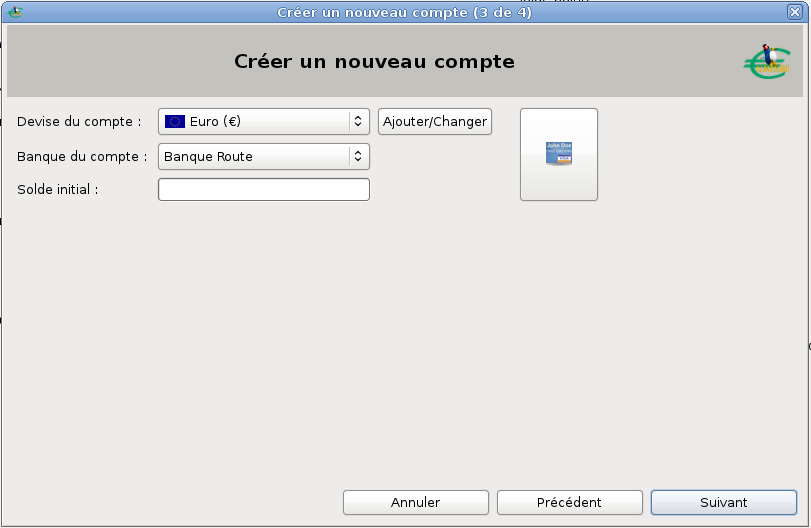
\includegraphics[scale=0.5]{image/screenshot/account_new_creation}
	\end{center}
	\caption{Création d'un nouveau compte}
	\label{account-new-creation-img}
	\end{figure}
	% image centrée
	\fi
	
		\begin{enumerate}
			\item choisissez la \indexword{devise}\index{devise} du compte dans la liste déroulante, qui propose les devises que connaît déjà votre fichier de comptes ; sinon, cliquez sur \menu{Ajouter/Changer}, une fenêtre s'affiche, où une liste déroulante vous propose toutes les devises du monde connues par Grisbi ; les détails de la devise sélectionnée s'affichent en-dessous, dans des champs que vous pouvez encore modifier ; puis validez par le bouton \menu{Fermer},
			\item choisissez la \indexword{banque}\index{banque !création} qui détient ce compte dans la liste déroulante, qui propose les banques que connaît déjà votre fichier de comptes ; sinon, cliquez sur \menu{Ajouter une nouvelle banque} : une fenêtre s'affiche, où vous pouvez renseigner le nom de la banque et de nombreux autres détails ; puis validez par le bouton \menu{Fermer},
			\item choisissez l'\indexword{icône}\index{icône} du compte : une fenêtre s'affiche, où vous pouvez soit choisir un répertoire dans la liste déroulante puis cliquer sur une des icônes en-dessous, soit chercher un fichier dans le système de fichiers de votre ordinateur (bouton \menu{Parcourir}) ; une fois votre icône trouvée, validez par le bouton \menu{Valider},
			\item saisissez le solde initial, puis validez par le bouton \menu{Suivant} ;
% espace pour Note ou Attention à la ligne dans une liste

\textbf{Note} : il est conseillé de laisser le solde initial du compte à zéro et, si besoin est, de créer par la suite une opération initiale du montant nécessaire, car cela facilitera la gestion future des rapprochements.
		\end{enumerate}

	\item saisissez le nom du \ifIllustration compte, celui qui apparaîtra dans le panneau de navigation, puis validez par le bouton \menu{Fermer}\refimage{account-new-name-img} ;
	\else compte, qui apparaîtra dans le panneau de navigation, puis validez par le bouton \menu{Fermer} ;
	\fi

	\ifIllustration
	% image centrée
	\begin{figure}[htbp]
	\begin{center}
	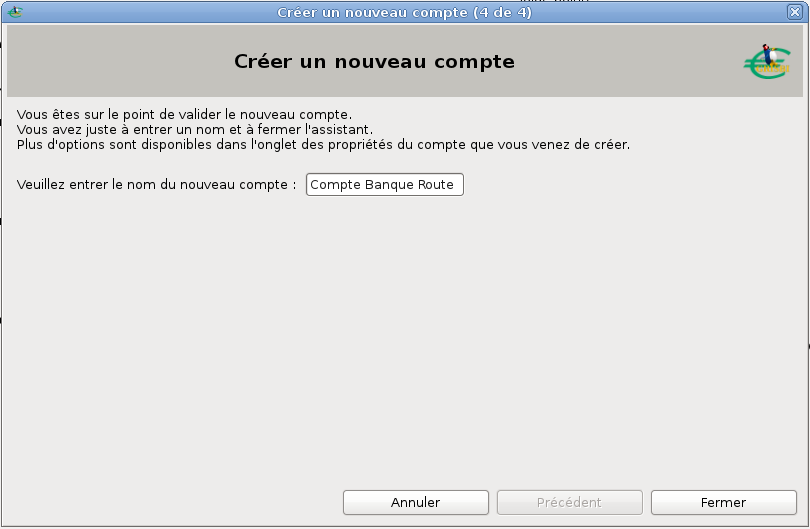
\includegraphics[scale=0.5]{image/screenshot/account_new_name}
	\end{center}
	\caption{Saisie du nom du nouveau compte}
	\label{account-new-name-img}
	\end{figure}
	% image centrée
	\fi
	\item le nouveau compte est alors créé, sélectionnez-le dans le panneau de navigation : son nom apparaît sur fond bleu{\couleur}, le pavé des détails affiche son onglet \menu{Opérations} qui est évidemment vide, et vous pouvez modifier ou compléter son onglet \menu{Propriétés}.
\end{enumerate}

%espace pour changement de thème
\vspacepdf{5mm}
Si, et seulement si vous venez de créer votre fichier de comptes juste avant cette création de compte, revenez à la fin de la section \vref{start-newfile-end}, \menu{Création d'un nouveau fichier de comptes}. Allez juste après la fin de la procédure de création du fichier de comptes, au paragraphe commençant par \emph{D'une manière ou d'une autre\ldots{ }}, ce qui vous proposera de créer tout de suite d'autres comptes.

%espace pour changement de thème
\vspacepdf{5mm}
Sinon, vous pouvez commencer à utiliser le compte que vous venez de créer.

%espace pour changement de thème
\vspacepdf{5mm}
Vous pouvez aussi configurer précisément les modes de règlement des opérations de ce compte dans le menu \menu{Édition - Préférences} (voir la section \vref{setup-resources-modes}, \menu{Modes de règlement}).


\section{Modification d'un compte\label{accounts-modify} }


Pour modifier un compte, sélectionnez le compte dans le panneau de navigation ou avec la barre d'information, puis cliquez sur l'onglet \menu{Propriétés} dans le pavé \ifIllustration des détails\refimage{account-new-properties-img}.
\else des détails.
\fi

Les champs suivants doivent obligatoirement être renseignés :
\begin{itemize}
	 \item le \menu{Nom du compte} ;
	 \item le \menu{Type du compte} ;
	 \item la \menu{Devise du compte} ;
	 \item le \menu{Solde initial}.
\end{itemize}
Tous les autres champs sont facultatifs. 


Vous pourrez modifier à tout moment \emph{toutes} ces informations, sauf la devise si vous avez choisi l'euro, ou si vous avez converti en euro un compte
existant, comme indiqué dans la section \vref{accounts-switcheuro}, \menu{Conversion d'un compte en euros}.

Les champs \menu{Type du compte}, \menu{Devise du compte}, \menu{Établissement financier} donnent accès à une liste déroulante permettant de renseigner le champ.

Les champs de texte peuvent être remplis au clavier, et un menu contextuel accessible par un clic-droit dans un champ de saisie permet d'effectuer les actions suivantes :
\begin{itemize}
	 \item \menu{Couper} (la sélection) ;
	 \item \menu{Copier} (la sélection) ;
	 \item \menu{Coller} (la sélection) ;
	 \item \menu{Supprimer} (la sélection) ;
	 \item \menu{Tout sélectionner} (dans le champ de saisie) ;
	 \item \menu{Méthodes de saisie} ;
	 \item \menu{Insérer un caractère de contrôle Unicode}\index{caractère de contrôle Unicode}.
\end{itemize}

%espace pour changement de thème
\vspacepdf{5mm}
Les \indexword{\gls{methodes de saisie}}\index{méthodes de saisie} permettent de changer les caractères accentués.

\indexword{Insérer un \gls{caractere de controle Unicode}} permet d'insérer un code Unichar qui modifie la présentation ; par exemple RLO (forçage droite-à-gauche) renverse l'ordre des lettres et la position du texte.

% espace avant Attention ou Note  : 5 mm
\vspacepdf{5mm}
\strong{Attention} : si vous modifiez certaines propriétés comme le type du compte, cela  nécessitera d'adapter aux nouvelles propriétés du compte, individuellement, toutes les opérations déjà saisies. Dans tous les cas, avant de procéder à une quelconque modification des comptes, faites \textbf{impérativement} une sauvegarde de votre fichier de comptes.

\ifIllustration
\else
% saut de page pour titre solidaire
\newpage
\fi

\section{Suppression d'un compte\label{accounts-delete} }


Pour supprimer un compte, cliquez sur le menu \menu{Édition - Supprimer le
compte courant}. Une boîte de dialogue de confirmation s'ouvre ; si
c'est vraiment ce que vous voulez, validez la suppression.

% espace avant Attention ou Note  : 5 mm
\vspacepdf{5mm}
\strong{Attention} : il n'y aura pas d'autre avertissement, et le compte est supprimé (ainsi que toutes ses opérations). Cette opération est \indexword{irréversible}\index{opération !irréversible} !


\section{Types de compte de Grisbi\label{accounts-type}}


Comme énoncé en début de chapitre, Grisbi sait gérer quatre \indexword{types de compte}\index{types de compte} :

\begin{itemize}
	\item compte bancaire : il permet de faire tout type d'opération ;
	\item compte de caisse : il ne permet de gérer que des espèces ;
	\item compte de passif : il permet de gérer une dette que vous remboursez ; 
	\item compte d'actif : il permet de gérer un bien qui se déprécie avec le temps. 
\end{itemize}

%espace pour changement de thème
\vspacepdf{5mm}
Cette section décrit les fonctionnalités et l'utilisation de chacun de ces types de compte.


\subsection{Type compte bancaire\label{accounts-type-bank}}

Le type de compte \emph{compte bancaire} admet tous les types d'opérations, en débit ou en crédit. De ce fait, il doit être utilisé pour tous les comptes suivants :
\begin{itemize}
	\item compte bancaire ou compte courant ;
	\item compte d'épargne ;
	\item compte de	\indexword{carte bancaire à débit immédiat}\index{carte bancaire !débit immédiat} ;
	\item compte de \indexword{carte de crédit}\index{carte bancaire !de crédit} ;		
	\item compte d'attente ;
	\item compte d'avances. 
\end{itemize}

Les paragraphes suivants décrivent ces comptes qui doivent utiliser le type de compte \emph{compte bancaire}.


\subsubsection{Compte bancaire, courant, d'épargne ou de carte bancaire à débit immédiat\label{accounts-type-bank-misc}}

Ces comptes servent à enregistrer toutes les opérations que vous pouvez faire avec votre banque : 

\begin{itemize}
	\item virement de compte à compte ;
	\item prélèvement sur le compte ;
	\item émission et dépôt de chèques ; 
	\item achat, remboursement, retrait et dépôt avec une \indexword{carte bancaire à débit immédiat}\index{carte bancaire !débit immédiat}. 
\end{itemize}


\subsubsection{Compte de carte de crédit\label{accounts-type-bank-creditcard}}

Un compte de carte de crédit est un compte de carte bancaire qui peut recevoir du débit, mais aussi du crédit, soit sous forme de virement, soit sous forme de prêt (par ex. un crédit renouvelable). Son solde peut donc être positif ou négatif.


\subsubsection{Compte d'attente\label{accounts-type-bank-waiting}}

Un compte d'attente sert à enregistrer des opérations (normalement des recettes) en attendant de les virer vers un compte bancaire ou de caisse. Il est normalement créditeur, jusqu'au moment du virement vers le compte bancaire ou de caisse, qui le ramène à un solde nul.

La \indexword{remise de chèques}\index{remise !chèques} et la \indexword{remise d'espèces}\index{remise !espèces} sont des exemples-type de l'utilité du compte d'attente. 
 
\paragraph{\textsl{Remise de chèques ou d'espèces  :}\label{accounts-type-bank-waiting-remittance}}

Si vous recevez peu ou peu souvent de chèques (ou d'espèces), le plus simple est de les saisir directement dans votre compte bancaire (ou dans votre compte de caisse). Dans ce cas, reportez-vous à la section \vref{transactions-new-cheque}, \menu{Remise de chèques ou d'espèces}.

% espace pour changement de thème
\vspacepdf{5mm}
Mais si vous recevez beaucoup de chèques (par exemple parce que vous gérez une association et que vos adhérents payent leur cotisation par chèque), le plus efficace est d'utiliser un compte d'attente.

% espace pour changement de thème
\vspacepdf{5mm}
La méthode consiste donc à créer un \emph{compte d'attente}, que vous nommez par exemple \emph{Chèques à encaisser}. Au fur et à mesure de la réception des chèques, vous les enregistrez individuellement dans ce compte, donc chaque chèque correspond à un \menu{Tiers}. Quand vous déposez les chèques à la banque, vous faites un virement de ce compte \emph{Chèques à encaisser} vers votre compte bancaire, du montant de l'ensemble de ces chèques, donc du solde du compte \emph{Chèques à encaisser}. Utilisez pour l'occasion un tiers \emph{Remise de chèques}, et dans le champ \menu{Remarques}, saisissez le numéro de votre bordereau de remise.
% (ce bordereau sera généré directement par Grisbi dans une prochaine version). 

Le solde du compte \emph{Chèques à encaisser} revient alors à zéro, et le compte bancaire est crédité du montant de la remise, exactement comme le sera votre relevé bancaire. Ainsi vous gardez et l'information du tiers pour chaque chèque, et celle de la remise globale.

Vous faites ensuite un pseudo-rapprochement du compte \emph{Chèques à encaisser} en simulant un relevé de solde nul avant la prochaine réception d'un chèque : vérifiez que ce rapprochement a bien un numéro, ou donnez-en lui un, par exemple REM-01, ce qui vous permettra ultérieurement de retrouver quel chèque faisait partie de quelle remise. Ce pseudo-rapprochement est appelé \emph{\indexword{lettrage}}\index{lettrage}.

% l'édition du bordereau de remise comportant \textbf{toutes} les opérations non-rapprochées (\emph{non fonctionnel pour l'instant, vous devrez créer ce bordereau à la main ou avec un logiciel de traitement de texte}).

%espace pour changement de thème
\vspacepdf{5mm}
Par exemple, si vous avez reçu deux chèques, vous enregistrez dans votre compte \emph{Chèques à encaisser} les deux opérations :

\begin{itemize}
	\item \menu{Date} : jj/mm/aa  \menu{Tiers} : Durand  \menu{Crédit} : 20  \menu{Catégorie} : \emph{Cotisations}  \menu{Mode de règlement} : \emph{Chèque}
	\item \menu{Date} : jj/mm/aa  \menu{Tiers} : Dupond  \menu{Crédit} : 40  \menu{Catégorie} : \emph{Cotisations}  \menu{Mode de règlement} : \emph{Chèque}
\end{itemize}

Puis lors de la remise des deux chèques à la banque, dans votre compte bancaire, vous enregistrez l'opération :

\begin{itemize}
	\item \menu{Date} : jj/mm/aa  \menu{Tiers} : Remise de chèques  \menu{Crédit} : 60  \menu{Catégorie} : \emph{Virement : Chèques à encaisser}  \menu{Mode de règlement} : \emph{Chèque}
\end{itemize}

\textbf{Note} : vous pouvez enregistrer cette opération soit dans votre compte bancaire en \menu{Crédit} et \menu{Catégorie} : \emph{Virement : Chèques à encaisser}, soit dans votre compte \emph{Chèques à encaisser} en \menu{Débit} et \menu{Catégorie} : \emph{Virement : Compte bancaire} ; dans les deux cas, Grisbi crée automatiquement la contre-opération dans l'autre compte.

Le compte \emph{Chèques à encaisser} est alors soldé à zéro, mais il garde la trace des chèques déposés à la banque, et dans votre compte bancaire n'apparaît que le montant global du bordereau de remise, que vous pourrez pointer avec votre relevé de compte de la banque.

%espace pour changement de thème
\vspacepdf{5mm}
Bien entendu, si une partie de vos adhérents vous paye en espèces, vous pouvez utiliser de la même façon un compte nommé par exemple \emph{Remise d'espèces}.


\subsubsection{Compte d'avances\label{accounts-type-bank-advance}}

Un compte d'avances sert à enregistrer à la fois les avances que vous recevez et celles que vous consentez. Il peut s'agir, par exemple, d'une avance sur votre salaire ou d'un achat que vous faites pour le compte d'un de vos amis.

% espace avant Attention ou Note  : 5 mm
\vspacepdf{5mm}
\textbf{Note} : le compte d'avances peut être déroutant pour le novice, puisqu'il fonctionne à l'envers, comme vous le découvrirez plus loin. Pour vous faciliter les choses, vous pouvez considérer que le compte d'avances se comporte comme un tiers qui vous donne ou à qui vous donnez de l'argent.

\paragraph{\textsl{Réception d'une avance  :}} quand vous \indexword{recevez une avance}\index{avance !réception}, vous enregistrez l'opération par un virement du compte d'avances vers un compte bancaire. Le tiers sera la personne ou l'organisation de qui vous recevez l'avance, et la catégorie sera \emph{Virement : Compte bancaire}. Dans le champ \menu{Notes}, vous indiquez le motif de l'avance. Le compte d'avances est donc débiteur quand vous devez de l'argent. Lorsque vous remboursez cette avance, vous faites un virement du compte bancaire, avec le même tiers et la même remarque, vers le compte d'avances, dont le solde redevient nul.

Pour une avance en espèces, remplacez le compte bancaire par un compte de caisse.

Dans le cas où l'avance vous est versée par chèque, et si vous avez créé un compte d'attente \emph{Chèques à encaisser}, vous devrez d'abord enregistrer le chèque dans le compte d'avances, puis faire un virement du montant du chèque, du compte d'avances vers ce compte \emph{Chèques à encaisser}, et ensuite faire votre virement de remise de chèque, de ce compte \emph{Chèques à encaisser} vers votre compte bancaire (voir le paragraphe \vref{accounts-type-bank-waiting}, \menu{Compte d'attente}). 

Vous ferez ensuite un rapprochement du compte d'avances pour faire disparaître ces opérations.

\paragraph{\textsl{Consentement d'une avance  :}} inversement, si vous \indexword{consentez une avance}\index{avance !consentement}, vous enregistrez l'opération par un virement d'un compte bancaire vers le compte d'avances. Le tiers sera la personne ou l'organisation à qui vous faites l'avance, et la catégorie sera \emph{Virement : Compte d'avances}. Dans le champ \menu{Remarques}, vous indiquerez le motif de l'avance. Le compte d'avances est donc créditeur quand on vous doit de l'argent. Lorsque cette avance vous est remboursée, vous enregistrez l'opération par un virement du compte d'avances vers le compte bancaire, avec le même tiers et la même remarque, et la catégorie sera \menu{Virement : Compte bancaire}. Le solde de votre compte d'avances redevient nul.

Pour une avance en espèces, remplacez le compte bancaire par un compte de caisse.

Dans le cas où l'avance vous est remboursée par chèque, et si vous avez créé un compte d'attente  \emph{Chèques à encaisser}, vous devrez d'abord enregistrer le chèque dans le compte d'avances, puis faire un virement du montant du chèque, du compte d'avances vers ce compte \emph{Chèques à encaisser}, et ensuite faire votre virement de remise de chèque, de ce compte \emph{Chèques à encaisser} vers votre compte bancaire  (voir le paragraphe \vref{accounts-type-bank-waiting}, \menu{Compte d'attente}). 

Vous ferez ensuite un rapprochement du compte d'avances pour faire disparaître ces opérations.

%espace pour changement de thème
\vspacepdf{5mm}
Un compte d'avances vous permet donc de vérifier facilement si vos créances ou vos dettes sont éteintes. Sans cette méthode cette vérification est difficile, sinon impossible.

% espace avant Attention ou Note  : 5 mm
\vspacepdf{5mm}
\textbf{Note} : lorsque vous faites un état des recettes et dépenses, ces opérations devraient être \emph{transparentes}, puisqu'elles s'annulent deux à deux quand chaque avance est remboursée. En pratique, lors de l'édition de ce genre d'état, vous devrez le configurer pour qu'il ne prenne pas en compte les virements entre comptes, et ainsi ces opérations seront totalement invisibles (voir la section \vref{reportscreation-selection-transfer}, \menu{Virements}).

% espace avant Attention ou Note  : 5 mm
\vspacepdf{5mm}
\textbf{Note} : lorsque vous créez un nouveau compte, choisissez donc de préférence le type de compte \emph{compte bancaire}, sauf si votre nouveau compte devra avoir une utilisation plus spécifique comme celles décrites dans les paragraphes ci-dessous.


\subsection{Type compte de caisse\label{accounts-type-cash}}

Le type de compte \emph{compte de caisse} est destiné uniquement aux opérations réglées en espèces ; vous ne pouvez pas y sélectionner de mode de paiement et il ne peut en aucun cas devenir négatif. De ce fait, il doit être utilisé pour tous les comptes suivants :
\begin{itemize}
	\item compte de caisse ;
	\item porte-monnaie électronique. 
\end{itemize}

% espace pour changement de thème  : 5 mm
\vspacepdf{5mm}
Un compte de caisse permet d'enregistrer dans votre comptabilité les retraits de la banque, pour alimenter la caisse, et les recettes et dépenses en espèces. En ce qui concerne les dépenses, il n’est pas toujours possible ni même utile d’enregistrer toutes les menues dépenses. Mais vous pouvez les enregistrer globalement, par exemple en fin de mois, dans des catégories adéquates ou bien dans une catégorie \menu{Dépenses diverses}, ceci afin de vider ce compte de caisse. Comme ceci, vous n’aurez pas de flou dans la caisse.

Un compte de caisse accepte les virements en provenance d'autres comptes. Lorsque vous faites un retrait en espèces sur votre compte bancaire, enregistrez-le en tant que virement vers le compte de caisse.


\subsection{Type compte de passif\label{accounts-type-liabilities}}

Le type de compte \emph{compte de passif} est un compte qui représente une dette, par exemple un \indexword{emprunt}\index{emprunt}. De ce fait, il doit être utilisé pour tous les comptes suivants :

\begin{itemize}
	\item compte d'emprunt ;
	\item compte de \indexword{carte bancaire à débit différé}\index{carte bancaire !débit différé}.
	
\end{itemize}


\subsubsection{Compte d'emprunt\label{accounts-type-liabilities-loan}}

Un compte d'emprunt sert à gérer un emprunt. Son solde initial est nul, mais, dès que vous contractez une dette, il devient négatif du montant de cette dette, et augmente ensuite à chaque remboursement versé, pour devenir nul après son dernier remboursement. 

En pratique, le solde initial de ce compte est nul, mais il devient (fortement) négatif dès la première opération, à savoir le virement, par l'organisme de crédit, du montant de l'emprunt sur votre compte courant. Vous enregistrez à ce moment-là un virement du compte de passif vers ce compte courant, ce qui vous permet de procéder à votre achat.

Par exemple, quand l'organisme de crédit Crédit Bitoire vous verse le montant de 20 000 pour acheter chez Auto Matique une voiture qui coûte 25 000, vous créez un compte de passif appelé \emph{Emprunt}, et dans ce compte, vous saisissez l'opération suivante : 

\begin{itemize}
	\item \menu{Date} : jj/mm/aa  \menu{Tiers} : Crédit Bitoire  \menu{Débit} : 20 000  \menu{Catégorie} : \emph{Virement : Banque Yze} \menu{Remarques} : Dette emprunt Crédit Bitoire
\end{itemize}

\textbf{Note} : si ce virement est fait directement par l'organisme de crédit sur le compte du vendeur, la catégorie devra être, par exemple, \emph{Virement : Compte Immobilisation}; vous pouvez n'avoir qu'un seul compte d'immobilisation pour tous vos biens, ou bien un compte par bien acheté.

%espace pour changement de thème
\vspacepdf{5mm}
À chaque fois que vous versez une échéance de votre \indexword{emprunt}\index{emprunt}, vous enregistrez un virement de votre compte courant vers le compte \emph{Emprunt}, du montant du capital remboursé, en catégorie \emph{Virement : Emprunt}, et une dépense sur ce compte courant, du montant des intérêts, en catégorie \emph{Frais financiers : Charges d'emprunts}. Éventuellement, ajoutez-y une dépense pour l'assurance, en catégorie \emph{Assurances}. De cette façon, vous saurez à tout moment le montant du capital restant à rembourser, mais aussi le coût de l'emprunt.

Par exemple, à chaque échéance, vous saisissez une opération ventilée sur votre compte courant :

\begin{itemize}
	\item opération maître  : \menu{Date} : jj/mm/aa  \menu{Tiers} : Crédit Bitoire  \menu{Débit} : 350  \menu{Catégorie} : \emph{Opération ventilée}
	\item 1\up{re} opération ventilée : \menu{Débit} : 300  \menu{Catégorie} : \emph{Virement : Emprunt}
	\item 2\up{e} opération ventilée : \menu{Débit} : 50  \menu{Catégorie} : \emph{Frais financiers : Charges d'emprunts}
\end{itemize}

%espace pour changement de thème
\vspacepdf{5mm}
N'oubliez pas que, si le montant de l'échéance est constant, à l'intérieur de chaque échéance suivante, le capital remboursé augmente et l'intérêt versé diminue (voir le tableau d'amortissement de l'emprunt).  

%espace pour changement de thème
\vspacepdf{5mm}
Vous pourrez donc parfaitement utiliser un compte de passif pour gérer vos emprunts ; comme Grisbi ne propose pas pour l'instant la ventilation automatique des remboursements d'emprunt (amortissements, intérêts et frais reportés automatiquement de votre tableau d'amortissement), vous pourrez tout de même saisir une opération planifiée et ventilée pour les remboursements, en mode manuel ou automatique, et vous ajusterez les montants à chaque échéance selon votre tableau (voir la section \vref{credit-amortization}, \menu{Tableau d'amortissement}).

%espace pour changement de thème
\vspacepdf{5mm}
Lorsqu'un compte de passif est soldé, ce qui signifie que vous avez remboursé la dette correspondante, Grisbi vous prévient en affichant un message dans la partie inférieure du pavé des détails de la page d'accueil (voir le chapitre \vref{home}, Accueil). 


\subsubsection{Compte de carte bancaire à débit différé\label{accounts-type-cash-deferredCards}}

Les cartes bancaires à débit différé peuvent être gérées de différentes manières, mais il est préférable de les gérer dans un compte spécifique, qui sera de type compte de passif, puisque leur solde ne peut pas être positif.

Vous trouverez tous les détails pour gérer correctement ces cartes bancaires dans la section \vref{bankcard-deferredCard}, \menu{Carte bancaire à débit différé}.


\subsection{Type compte d'actif\label{accounts-type-assets}}

Le type de compte \emph{compte d'actif} est un compte qui représente un bien, par exemple une voiture. Son solde initial est nul, mais il devient positif dès que vous possédez ce bien, d'un montant égal à sa valeur, puis il diminue avec le temps à mesure de sa dépréciation, pour finir à une valeur nulle. Les opérations se font par virement. On peut le considérer comme le  contraire d'un compte de passif.

%espace pour changement de thème
\vspacepdf{5mm}
En pratique, le solde initial de ce compte est nul, mais il devient (fortement) positif dès la première opération, à savoir l'achat de ce bien. Vous enregistrez à ce moment-là un virement de votre compte courant vers ce \indexword{compte d'actif}\index{actif !compte}, égal au prix d'achat du bien, ce qui vous permet de procéder à votre achat.

Par exemple, quand vous achetez la voiture à 25 000 chez Auto Matique, vous créez un compte d'actif appelé \emph{Compte Immobilisation}, et dans votre compte courant, vous saisissez l'opération suivante : 

\begin{itemize}
	\item \menu{Date} : jj/mm/aa  \menu{Tiers} : Auto Matique  \menu{Débit} : 25 000  \menu{Catégorie} : \menu{Virement : Compte Immobilisation}  \menu{Remarques} : Actif achat voiture
\end{itemize}

Votre compte \emph{Immobilisation} enregistre donc une opération en crédit, du montant de cette voiture.

%espace pour changement de thème
\vspacepdf{5mm}
À chaque fois que vous constatez une \indexword{dépréciation}\index{dépréciation !actif}\index{actif !dépréciation} de ce bien, vous enregistrez un retrait du compte d'actif, du montant de la dépréciation, dans la catégorie \emph{Amortissements : Dépréciation}. Ces retraits pourront être faits jusqu'à ce que le solde du compte soit nul. De cette façon vous connaîtrez en permanence la valeur de votre bien.

Par exemple, au bout d'un an la cotation de votre voiture (par ex. dans votre journal préféré) a perdu une certaine valeur ; dans votre compte \emph{Immobilisation}, vous saisissez l'opération suivante : 

\begin{itemize}
	\item \menu{Date} : 31/12/2012  \menu{Tiers} : Dépréciation Voiture  \menu{Débit} : 5000  \menu{Catégorie} : Amortissements : Dépréciation
\end{itemize}

%espace pour changement de thème
\vspacepdf{5mm}
Lors de l'achat, le montant que vous possédez réellement est votre apport personnel. Au cours du temps, vous remboursez les mensualités de votre emprunt, tandis que votre bien se déprécie. Le solde des comptes d'actif et de passif vous donnera à tout moment le montant que vous possédez globalement.


\section{Conversion d'un compte en euros\label{accounts-switcheuro}}


Cette section devient de plus en plus obsolète au fur et à mesure que le 
temps passe, mais nous la maintenons encore pour vous permettre l'éventuel
import de vieux fichiers de compte.

Cette fonction n'existe plus à partir de la version 0.8 de Grisbi. Donc, si vous avez absolument
besoin de réaliser cette opération, le seul moyen serait de la faire en utilisant une version précédente, de la manière suivante :

% espace avant Attention ou Note  : 5 mm
\vspacepdf{5mm}
\strong{Attention} : cette procédure n'est qu'une proposition, et n'a pas été
testée avec toutes les versions précédentes de Grisbi. C'est pour cela qu'il est
de la plus haute importance de sauvegarder auparavant votre fichier de comptes en lieu sûr.

\begin{enumerate}
	 \item avant tout, faites une copie de votre fichier de comptes actuel, renommez-le (par ex. en \file{comptesSauvegarde.gsb)} et placez-le en lieu sûr ;
	 \item choisissez une version ancienne de Grisbi, la moins ancienne possible 	et qui dispose de la fonction de conversion en euros ; vous devriez pouvoir la trouver, ainsi que son manuel, à la page du site de \lang{Grisbi}\footnote{\urlGrisbi{}} ; installez-la ;
	 \item importez le compte voulu en suivant les instructions du manuel de cette ancienne version de Grisbi que vous venez d'installer ;
	 \item procédez à la conversion de ce compte en euros ;
	 \item exportez ce compte en suivant les instructions du même manuel ; vous obtenez alors un fichier d'export ;
	 \item redémarrez votre nouvelle version de Grisbi et ouvrez votre fichier de comptes habituel (pas la sauvegarde, évidemment !) ;
	 \item procédez à l'importation du fichier d'export ;
	 \item si tout se passe bien, vous disposez maintenant de votre compte converti en euros.
\end{enumerate}

% espace avant Attention ou Note  : 5 mm
\vspacepdf{5mm}
\strong{Attention} : d'une manière générale, il est déconseillé d'avoir des accents ou des espaces dans les noms des répertoires et fichiers utilisés par Grisbi. Si c'est le cas, renommez-les maintenant. Par exemple, les espaces peuvent être remplacées par des tirets bas (\_). 


\myclearemptydoublepage

%%%%%%%%%%%%%%%%%%%%%%%%%%%%%%%%%%%%%%%%%%%%%%%%%%%%%%%%%%%%%%%%%
% Contents : The transactions chapter
% $Id : grisbi-manuel-transactions.tex,v 0.4 2002/10/27 Daniel Cartron
% $Id : grisbi-manuel-transactions.tex, v 0.5.0 2004/06/01 Loic Breilloux
% some of its content was in tips chapter  : 
% $Id : grisbi-manuel-tips.tex, v 0.4 2002/10/27 Daniel Cartron
% $Id : grisbi-manuel-transactions.tex, v 0.6.0 2011/11/17 Jean-Luc Duflot
% some of its content was in tips chapter :
% $Id : grisbi-manuel-tips.tex, v 0.5.0 2004/06/01 Loic Breilloux
% $Id : grisbi-manuel-transactions.tex, v 0.8.9 2012/04/27 Jean-Luc Duflot
% $Id : grisbi-manuel-transactions.tex, v 1.0 2014/02/12 Jean-Luc Duflot
% some of its content was in accounts chapter :
% $Id : grisbi-manuel-accounts.tex, v 0.8.9 2012/04/27 Jean-Luc Duflot
%%%%%%%%%%%%%%%%%%%%%%%%%%%%%%%%%%%%%%%%%%%%%%%%%%%%%%%%%%%%%%%%%

\chapter{Opérations d'un compte\label{transactions}}

Les différents comptes que vous avez créés contiennent les opérations. Pour afficher la liste des comptes enregistrés dans votre fichier de comptes, utilisez la barre d'information ou le panneau de navigation (voir le chapitre \vref{home}, \menu{Accueil} et la section \vref{accounts-list}, \menu{Liste des comptes}).

Pour afficher les opérations d'un compte, sélectionnez ce compte dans la liste : l'onglet \menu{Opérations} s'affiche par défaut. Il possède quatre éléments principaux :

\begin{itemize}
	 \item la barre d'outils ;
	 \item la liste des opérations ;
	 \item le formulaire de saisie des opérations ;
	 \item le \indexword{solde pointé}\index{solde !pointé}.
\end{itemize}

% espace avant Attention ou Note  : 5 mm
\vspacepdf{5mm}
\textbf{Note} : si vous n'avez jamais fait de rapprochement, donc pas de pointages, Grisbi ne peut ni calculer ni afficher de solde pointé.


\section{Barre d'outils\label{transactions-functions}}


La barre d'outils présente les fonctions suivantes  : 

\begin{itemize}
	 \item \menu{Nouvelle Opération} : va à la fin de la liste des opérations et ouvre le formulaire de saisie vierge ;
	 \item \menu{Supprimer} : supprime l'opération sélectionnée ;
	 \item \menu{Éditer} : ouvre le formulaire de saisie pour l'opération sélectionnée et permet de la modifier ;
	 \item \menu{Rapprocher} : ouvre la page de rapprochement du compte sélectionné (voir le chapitre \vref{reconciliation}, \menu{Rapprochement bancaire}) ;
	 \item \menu{Imprimer} : ouvre la fenêtre de sélection de l'imprimante et de ses
	options ;
	 \item \menu{Affichage} : ouvre un menu déroulant ; vous pouvez choisir l'\indexword{affichage des opérations}\index{affichage !opérations} parmi quatre possibilités (\menu{Vue simple}, \menu{Mode \og deux lignes \fg{}}, \menu{Mode \og trois lignes \fg{}} et \menu{Vue complète}), ainsi que l'affichage ou non des \indexword{opérations rapprochées}\index{affichage !opérations rapprochées} et des \indexword{lignes d'archives}\index{affichage !lignes d'archives}.
\end{itemize}

% espace pour changement de thème
\vspacepdf{5mm}
Les options du menu \menu{Affichage} influent par défaut sur l'affichage de tous les comptes. Vous pouvez préférer un affichage différent pour chaque compte, cela est configurable dans le menu \menu{Édition - Préférences}  (voir le paragraphe \vref{setup-operations-list-differenciation}, \menu{Différenciation des comptes}).
 
% FONCTION SUPPRIMÉE La \indexword{barre d'outils}\index{barre d'outils !déplacement} peut être déplacée dans l'écran en cliquant sur sa poignée (petit rectangle vertical à gauche de la barre) et en la déplaçant. Pour la réattacher à son emplacement d'origine dans le pavé des détails, la remettre en haut de la fenêtre, le haut de la poignée sur le petit trait qui visualise sa place d'origine.


\section{Liste des opérations\label{transactions-list}}


\subsection{Description\label{transactions-list-description}}

La liste des opérations s'affiche dans le panneau des \ifIllustration détails\refimage{transactions-list-img}.
\else détails.
\fi

\ifIllustration 
% image centrée 
\begin{figure}[ht]
\begin{center}
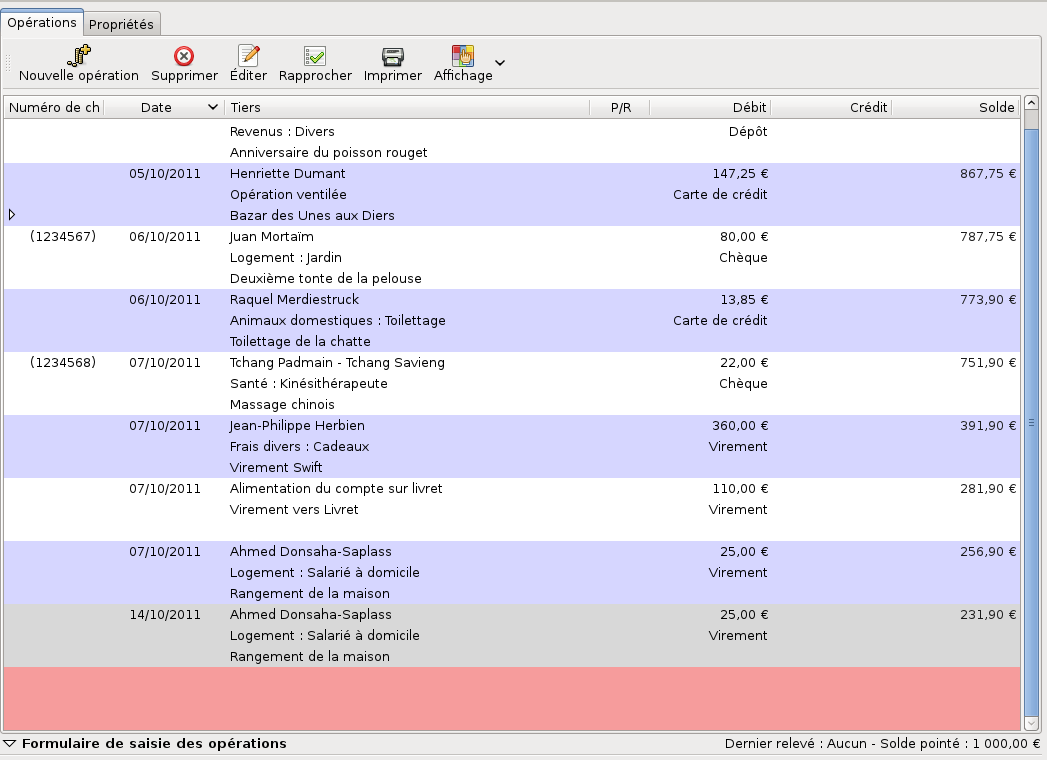
\includegraphics[scale=0.5]{image/screenshot/transactions_list}
\end{center}
\caption{Liste des opérations}
\label{transactions-list-img}
\end{figure}
% image centrée 
\fi

Elle affiche en haut la barre des libellés des colonnes. Vous pouvez \indexword{élargir ou rétrécir une colonne}\index{colonne !largeur} en cliquant sur le séparateur entre deux colonnes et en le déplaçant. Pour rétablir la largeur des colonnes à leur valeur par défaut, sélectionnez le menu \menu{Affichage - Réinitialiser la largeur des colonnes}.

Vous pouvez déplacer la liste des opérations vers le haut ou vers le bas avec la molette de la souris, ou bien avec la souris et l'ascenseur vertical. Le déplacement vers la gauche ou la droite se fait avec la souris et l'ascenseur horizontal.

Vous pouvez choisir d'afficher ou non les \indexword{opérations rapprochées}\index{affichage !opérations rapprochées} et les \indexword{lignes d'archives}\index{affichage !lignes d'archives} : sélectionnez \menu{Affichage - Montrer les opérations rapprochées} ou \menu{Affichage - Montrer les lignes d'archives} dans la barre de menus ou dans la barre d'outils (voir la section \vref{home-menus-display}, \menu{Menu Affichage} ou la fonction \menu{Affichage} dans la section \vref{transactions-functions}, \menu{Barre d'outils}).

% espace pour changement de thème
\vspacepdf{5mm}
Du point de vue de la base de données de Grisbi, une opération est constituée de ses \indexword{champs d'information}\index{champ d'information !définition}. Les champs d'information de chaque opération s'affichent dans les différentes \indexword{cellules}\index{cellule !champ d'information} définies par l'intersection des lignes et des colonnes. Il ne peut y avoir au  maximum que quatre lignes et sept colonnes, ce qui définit un maximum de vingt-huit champs d'information pour chaque opération.

Chaque opération peut être affichée sur 1, 2, 3 ou 4 lignes, suivant le mode d'affichage sélectionné (voir la section \vref{home-menus-display}, menu \menu{Affichage} dans la barre de menus ou la fonction \menu{Affichage} dans la section \vref{transactions-functions}, \menu{Barre d'outils}). L'affichage courant y est indiqué par une coche. 

Vous pouvez aussi configurer le contenu de ces lignes, ainsi que la mémorisation des réglages de l'affichage, individuellement pour chaque compte, dans le menu \menu{Édition - Préférences} (voir les sections \vref{setup-operations-list}, \menu{Comportement de la liste} et \vref{setup-operations-cells}, \menu{Cellules de la liste des opérations}).

Le \indexword{libellé d'une colonne}\index{colonne !libellé} est toujours le nom du champ d'information  affiché dans la première ligne des opérations.

Pour des raisons de lisibilité de l'affichage, Grisbi n'affiche aucune bordure aux cellules, colonnes, lignes et opérations, mais présente une alternance de couleurs de fond violet et blanc{\couleurs} à chaque ligne.


\subsection{Champs d'information et de saisie\label{transactions-list-fields}}

Grisbi sait gérer, pour chaque opération, une liste complète de champs d'information et de saisie\index{champs d'information}\index{champs de saisie}, qui sont les suivants :

\begin{itemize}
	\item \menu{Date de l'opération}\index{date !opération} : \indexword{date} à laquelle est réalisée l'opération ; elle peut être utilisée pour calculer les soldes ;
	\item \menu{Date de valeur}\index{date !valeur} : \indexword{date} à laquelle la banque comptabilise l'opération ; c'est cette date qui fait foi pour le calcul des intérêts et des agios ; elle peut être utilisée pour calculer les soldes ;
	\item \menu{Tiers} ;
	\item \menu{Imputation budgétaire} ;
	\item \menu{Débit} : montant débité du solde du compte ; dans le cas d'opérations dans une \indexword{devise différente}\index{devise !différente} de celle du compte, montant de l'opération dans la devise différente ;
	\item \menu{Crédit} ;
	\item \menu{Solde} : montant toujours calculé \emph{après} l'opération affichée sur la même ligne ; il dépend chronologiquement du \indexword{tri primaire}\index{tri !primaire} sélectionné ; un \indexword{solde négatif}\index{solde !négatif} est affiché en rouge{\couleur} ;
	\item \menu{Montant} : dans le cas d'opérations dans une \indexword{devise différente}\index{devise !différente} de celle du compte, montant de l'opération dans la devise du compte ;
	\item \menu{Moyen de paiement} ;
	\item \menu{\No rapprochement} : numéro de chaque rapprochement dans chaque compte ;
	\item \menu{Exercice} ;
	\item \menu{Catégorie} ;
	\item \menu{P/R} : statut de l'opération, \emph{Pointé} ou \emph{Rapproché} ;
	\item \menu{Pièce comptable}, par exemple le numéro de la facture (\menu{Pièce comptable} et \menu{Numéro d'opération} sont des références réciproques qui assurent la traçabilité de l'opération) ;
	\item \menu{Remarques} : informations éventuelles sur l'opération ;
	\item \menu{Infos banque/guichet}, utile uniquement si vous enregistrez un chèque reçu ;
	\item \menu{Numéro d'opération} : il s'agit d'un numéro d'ordre unique que Grisbi attribue à chaque opération ; vous pouvez reporter ce numéro sur la pièce comptable correspondante (\menu{Numéro d'opération} et \menu{Pièce comptable} sont des références réciproques qui assurent la traçabilité de l'opération) ;
	\item \menu{\No chèque} ou \menu{\No chèque/virement }, si le mode de règlement sélectionné permet cette saisie ;
	\item \menu{Devise de l'opération} ;
	\item \menu{Taux de change} ;
	\item \menu{Mode de règlement de la \indexword{contre-opération}}\index{contre-opération} : vous pouvez le configurer pour chaque compte dans le menu \menu{Édition - Préférences} (voir la section \vref{setup-resources-modes}, \menu{Modes de règlement}) ;
	\item \menu{Auto/Manuel} : statut de l'exécution d'une opération planifiée
\end{itemize}

% espace pour changement de thème
\vspacepdf{5mm}
La liste des opérations et le formulaire de saisie utilisent chacun un sous-ensemble de ces champs. Vous pouvez voir les deux listes complètes dans les tableaux du menu \menu{Édition - Préférences}, onglets \menu{Cellules de la liste des opérations} et \menu{Contenu}, ou dans les sections \vref{setup-operations-cells}, \menu{Cellules de la liste des opérations} et \vref{setup-form-content}, \menu{Contenu}.


\subsection{Gestion des champs d'information\label{transactions-list-fields-manage}}

Grisbi affiche par défaut, dans la liste des opérations, un certain nombre de ces champs (tiers, catégorie, débit, etc.). Mais vous pouvez aussi \indexword{gérer les champs d'information}\index{champ d'information !gestion} différemment, c'est à  dire afficher de nouveaux champs, les modifier ou en supprimer l'affichage, à votre convenance. 
Vous pouvez soit faire ces manipulations dans le menu \menu{Édition - Préférences - Opérations - Cellules de la liste des opérations}, qui offre un aperçu complet de la disposition des champs dans les cellules, et permet de faire plusieurs modifications facilement (voir la section \vref{setup-operations-cells}, \menu{Cellules de la liste des opérations}), soit le faire directement dans la liste des opérations, en suivant les méthodes ci-dessous :


\subsubsection{Ajout d'un champ d'information\label{transactions-list-fields-add}}

Pour \indexword{ajouter un champ d'information}\index{champ d'information !ajouter} dans une cellule, procédez comme suit :

\begin{enumerate}
	 \item sélectionnez \menu{Affichage - Vue complète} dans la barre d'outils ou \menu{Affichage - Montrer quatre lignes par opération} dans la barre de menus, pour vous assurer de voir toutes les vingt-huit cellules ;
	 \item cliquez-droit dans une des cellules vides de la colonne où vous voulez ajouter ce champ : faites-le précisément, car rien ne permet d'identifier sur quelle cellule vous avez cliqué ;
	 \item  un menu contextuel s'affiche ; sélectionnez \menu{Modifier le contenu de la cellule} ; vérifiez qu'il n'y a pas déjà de champ d'information dans cette cellule, en constatant qu'aucun champ de la liste déroulante n'a de coche à gauche de son nom ;
	 \item choisissez un champ d'information proposé dans la liste ; ce champ s'ajoute dans la cellule choisie, et toutes les opérations de la liste l'affichent.
\end{enumerate}


\subsubsection{Modification d'un champ d'information\label{transactions-list-fields-modify}}

Pour \indexword{modifier un champ d'information}\index{champ d'information !modifier} dans une cellule, procédez comme suit :

\begin{enumerate}
	 \item sélectionnez \menu{Affichage - Vue complète} dans la barre d'outils ou \menu{Affichage - Montrer quatre lignes par opération} dans la barre de menus, pour vous assurer de voir toutes les vingt-huit cellules ;
	 \item cliquez-droit dans une des cellules de la colonne dont vous voulez modifier le champ : faites-le précisément, car rien ne permet d'identifier sur quelle cellule vous avez cliqué ;
	 \item  un menu contextuel s'affiche ; sélectionnez \menu{Modifier le contenu de la cellule} ; le champ d'information actuel dans cette cellule est indiqué par une coche à gauche de son nom ;
	 \item choisissez un autre champ d'information proposé dans la liste ; ce champ remplace le précédent dans la cellule choisie, et toutes les opérations de la liste l'affichent.
\end{enumerate}


\subsubsection{Suppression d'un champ d'information\label{transactions-list-fields-remove}}

Pour \indexword{supprimer un champ d'information}\index{champ d'information !supprimer} dans une cellule, procédez comme suit :

\begin{enumerate}
	 \item sélectionnez \menu{Affichage - Vue complète} dans la barre d'outils ou \menu{Affichage - Montrer quatre lignes par opération} dans la barre de menus, pour vous assurer de voir toutes les vingt-huit cellules ;
	 \item cliquez-droit dans la cellule du champ à supprimer : faites-le précisément, car rien ne permet d'identifier sur quelle cellule vous avez cliqué ;
	 \item un menu contextuel s'affiche ; sélectionnez \menu{Modifier le contenu de la cellule} ; le champ d'information actuel dans cette cellule est indiqué par une coche à gauche de son nom ;
	 \item choisissez \menu{Effacer la cellule} dans la liste ; le champ d'information actuel disparaît pour toutes les opérations de la liste (mais les informations ne sont en aucun cas supprimées de votre fichier de comptes).
\end{enumerate}

\subsubsection{Déplacement d'un champ d'information\label{transactions-list-fields-move}}

Pour \indexword{déplacer un champ d'information}\index{champ d'information !déplacer}, vous pouvez le supprimer puis l'ajouter dans un autre champ vide, mais vous pouvez aussi le faire dans le menu \menu{Édition - Préférences - Opérations - Cellules de la liste des opérations}. Voir la section \vref{setup-operations-cells}, \menu{Cellules de la liste des opérations}.


\subsection{Tris\label{transactions-list-sorts}}

Pour changer l'ordre d'affichage des opérations, vous pouvez faire un \indexword{tri sur les opérations}\index{tri !opérations} sur un des champs d'information ; procédez comme suit :

\begin{enumerate}
	  \item cliquez-droit sur le libellé de la colonne qui contient le champ d'information choisi comme critère de \gls{tri} ;
	  \item un menu contextuel affiche la liste des champs de cette colonne ; 	sélectionnez le champ choisi comme critère de tri ;
	  \item toutes les opérations s'affichent, triées selon le critère choisi ;
	  \item un petit triangle noir apparaît à droite du libellé de la colonne ; il pointe vers le bas si le tri est ascendant, vers le haut si le tri est descendant ;
% saut de ligne pour indentation correcte de la note dans la liste

	  \textbf{Note} : ces triangles peuvent être remplacés, en fonction du thème de l'environnement de bureau ou du gestionnaire de fenêtres que vous utilisez, par d'autres caractères tels que +, -, >, <, etc.
	  \item cliquez sur ce triangle pour changer l'ordre du tri.
\end{enumerate}

\textbf{Note} : un tri sur l'affichage réalisé ainsi n'affecte en aucun cas le solde à chaque ligne, qui est calculé après chaque opération ; suivant le tri et les options d'affichage que vous avez choisi, le solde à chaque ligne peut présenter une évolution non chronologique. 

%espace pour changement de thème
\vspacepdf{5mm}
Vous pouvez aussi configurer l'ordre général des tris dans le menu \menu{Édition - Préférences} (voir la section \vref{setup-operations-list-modes}, \menu{Modes d'affichage}).

\textbf{Note} : le choix du critère de \gls{tri primaire} (date d'opération ou date de valeur) qui peut y avoir été fait modifie nécessairement le solde affiché à chaque ligne d'opération, puisque Grisbi calcule et affiche le solde à chaque ligne.


\section{Formulaire de saisie\label{transactions-form}}


Le formulaire de saisie est situé en-dessous de la liste des opérations, où une ligne affiche, à gauche de \menu{Formulaire de saisie des opérations}, un petit triangle qui  permet d'\indexword{afficher ou de masquer}\index{formulaire de saisie !masquer-afficher} \ifIllustration ce formulaire\refimage{transactions-form-img}.
\else ce formulaire.
\fi

\ifIllustration
% image centrée 
\begin{figure}[htbp]
\begin{center}
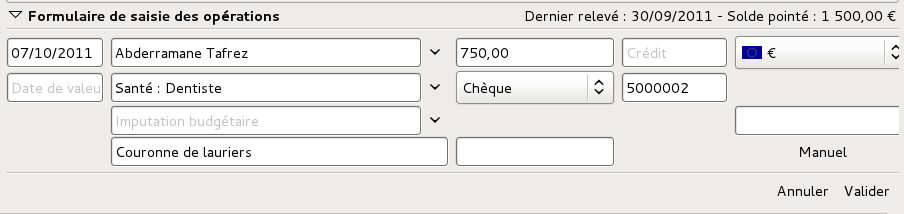
\includegraphics[scale=0.5]{image/screenshot/transactions_form}
\end{center}
\caption{Formulaire de saisie des opérations}
\label{transactions-form-img}
\end{figure}
% image centrée 
\fi

\textbf{Note} : ce triangle peut être remplacé, en fonction du thème de l'environnement de bureau ou du gestionnaire de fenêtres que vous utilisez, par d'autres caractères tels que +, -, >, <, etc.

Le formulaire de saisie comprend par défaut les sept champs suivants : \menu{Date de l'opération}, \menu{Tiers}, \menu{Débit}, \menu{Crédit}, \menu{Catégorie}, \menu{Moyen de paiement} et \menu{Remarques}. Vous pouvez avoir besoin de champs supplémentaires, par exemple \menu{Exercice}, \menu{Imputation budgétaire} ou autre. Pour cela, allez dans le menu \menu{Édition - Préférences - Formulaire des opérations - Contenu}, ou cliquez-droit dans le formulaire de saisie, dans une zone grise en dehors des champs de saisie, sélectionnez \menu{Configurer le formulaire} (voir la section \vref{setup-form}, \menu{Formulaire des opérations}).

%espace pour changement de thème
\vspacepdf{5mm}
Pour connaître l'ensemble des champs que peut gérer Grisbi, voir la section \vref{transactions-list-fields}, \menu{Champs d'information et de saisie}.

Une fois le formulaire affiché, un menu contextuel accessible par un clic-droit dans un champ de saisie permet d'effectuer les actions suivantes :

\begin{itemize}
	 \item \menu{Couper} (la sélection) ;
	 \item \menu{Copier} (la sélection) ;
	 \item \menu{Coller} (la sélection) ;
	 \item \menu{Supprimer} (la sélection) ;
	 \item \menu{Tout sélectionner} (dans le champ de saisie) ;
	 \item \menu{Méthodes de saisie}\index{méthodes de saisie} ;
	 \item \menu{Insérer un caractère de contrôle Unicode}\index{caractère de contrôle Unicode}.
\end{itemize}

%espace pour changement de thème
\vspacepdf{5mm}
Le choix \menu{\gls{methodes de saisie}} permet de changer les caractères accentués.

Le choix \menu{Insérer un \gls{caractere de controle Unicode}} permet d'insérer un code Unichar qui modifie la présentation ; par exemple RLO (forçage droite-à-gauche) renverse l'ordre des lettres et la position du texte.

De plus, un autre menu contextuel, accessible par un clic-droit en dehors d'un champ de saisie, permet d'accéder à la \indexword{configuration du formulaire}\index{formulaire de saisie !configuration} : vous pouvez en configurer précisément le contenu, la présentation, le comportement, ainsi que les paramètres d'aide à la saisie, dans le menu \menu{Édition - Préférences} (voir la section \vref{setup-form}, \menu{Formulaire des opérations}).


\section{Solde pointé\label{transactions-balance}}


En-dessous de la liste des opérations, sur la même ligne que le formulaire de saisie, s'affichent à droite deux informations  : la date du dernier relevé bancaire rapproché et le \indexword{solde pointé}\index{solde !pointé} correspondant à ce dernier rapprochement, à moins que vous ne pointiez très régulièrement vos opérations, auquel cas il correspond au solde tel que le connaît votre banque (voir le chapitre \vref{reconciliation}, \menu{Rapprochement bancaire}).

\ifIllustration
% saut de page pour titre solidaire
\newpage
\else
\fi


\section{Sélection d'une opération \label{transactions-selection}}


Pour sélectionner une opération, vous avez deux moyens :

\begin{itemize}
	 \item cliquez sur une de ses lignes ;
	 \item déplacez la sélection avec les touches du clavier \key{Flèche Haut} et \key{Flèche Bas}.
\end{itemize}

L'opération apparaît alors sur fond rouge{\couleur} et ses détails s'affichent dans le formulaire.

% espace pour changement de thème
\vspacepdf{5mm}
Un menu contextuel est disponible sur la liste des opérations. Un clic-droit sur la ligne d'une opération permet les fonctions suivantes, selon le contexte :
% espace avant image 5mm
\vspacepdf{3mm}

\begin{itemize}
	\ifIllustration
	% image entourée par une liste (picins)
	% Pas de référence à l'illustration car erreur de numéro de figure avec picins
	%supprimé car en html les figures entourées ne sont pas numérotées, et la numérotation des figures centrées décalée par rapport au pdf
	%\piccaption{Menu contextuel de la liste des opérations}
	\label{transactions-contextMenu-img}
	\parpic[r]{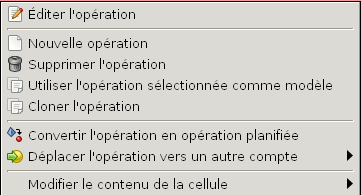
\includegraphics[scale=0.50]{image/screenshot/transactions_contextMenu}}
	% image entourée par une liste (picins)
	\fi
	 \item \menu{Afficher la contre-opération}\index{contre-opération !afficher} : ce choix est présent seulement si l'opération est un virement ;
	 \item \menu{Éditer l'opération} ;
	 \item \menu{Nouvelle opération} ;
	 \item \menu{Supprimer l'opération} ;
	 \item \menu{Utiliser l'opération sélectionnée comme modèle} ;
	 \item \menu{Cloner l'opération} ;
	 \item \menu{Convertir l'opération en opération planifiée} : cela permet de créer facilement des échéances après coup ;
	 \item \menu{Déplacer l'opération vers un autre compte} ;
	 \item \menu{Rechercher} : un montant ou une chaîne de caractères ; 
	 \item \menu{Modifier le contenu de la cellule}.
\end{itemize}


\section{Saisie d'une nouvelle opération\label{transactions-new}}


La saisie d'une opération se fait dans le formulaire de saisie, situé en-dessous de la liste des opérations.

Pour saisir une nouvelle opération, ouvrez ou affichez le formulaire de saisie avec l'une de ces méthodes :

\begin{itemize}
	 \item sélectionnez la ligne vide en bas de la liste des opérations et appuyez sur la touche \key{Entrée} ;
	 \item appuyez sur la combinaison de touches \key{Ctrl}\key{T} ;
	 \item double-cliquez sur la ligne vide ;
	 \item dans la barre de menus, sélectionnez \menu{Édition - Nouvelle opération} ;
	 \item dans la barre de menus, sélectionnez \menu{Montrer le formulaire de saisie d'opérations} ;
	 \item dans la barre d'outils, cliquez sur \menu{Nouvelle opération} ;
	 \item dans le menu contextuel, sélectionnez \menu{Nouvelle opération} ;
	 \item cliquez sur le petit triangle d'\indexword{affichage/masquage}\index{formulaire de saisie !masquer-afficher} du formulaire de saisie des opérations à gauche de son libellé.
% saut de ligne pour indentation correcte de la note dans la liste

	 \textbf{Note} : ce triangle peut être remplacé, en fonction du thème de l'environnement de bureau ou du gestionnaire de fenêtres que vous utilisez, par d'autres caractères tels que +, -, >, <, etc.
\end{itemize}

% espace après Attention ou Note  : 5 mm
\vspacepdf{5mm}
La dernière ligne, entièrement vide, en bas de la liste des opérations, apparaît sur fond rouge{\couleur}, le formulaire de saisie vierge s'affiche, avec seule la date du jour, ou la dernière date entrée, sur fond bleu{\couleur}.

% espace pour changement de thème
\vspacepdf{5mm}
Saisissez les différentes informations concernant votre opération dans les différents champs du formulaire. Certains champs peuvent être renseignés soit avec le clavier, soit avec une liste déroulante. Si vous utilisez le clavier, cette saisie sera automatiquement enregistrée dans la liste déroulante de ce champ. Si vous le voulez, vous pourrez toujours supprimer plus tard ce choix dans la liste : reportez-vous aux différents chapitres traitant de ces listes (\menu{Tiers}, \menu{Catégories}, \menu{Imputations budgétaires} et les différents onglets de la section \menu{Ressources} du menu \menu{Édition - Préférences}.

Chaque champ de saisie doit être renseigné par le type de  donnée qui lui convient (date, nombre, texte), sinon l'arrière-plan du champ deviendra rouge{\couleur}. 

Une fois le dernier champ du formulaire saisi et validé, l'opération s'affiche dans la liste des opérations, et la ligne active, en rouge{\couleur}, passe à la dernière ligne vide de la liste.

% espace pour changement de thème
\vspacepdf{5mm}
Les sous-sections suivantes donnent les différentes méthodes de saisie disponibles.


\subsection{Commandes principales au clavier\label{transactions-new-keyboard}}

La touche \key{Tabulation} permet le déplacement dans le formulaire.

La touche \key{Entrée} permet soit de se déplacer dans le formulaire de saisie, soit de valider la saisie ; cela est configurable dans le menu \menu{Édition - Préférences} (voir la section \vref{setup-form-behaviour}, \menu{Comportement}). Cette  configuration affecte à la fois la touche \key{Entrée} du clavier alphabétique et celle du pavé numérique.

La touche \key{Échap} permet d'annuler la saisie en cours.


\subsection{Saisie de date au clavier\label{transactions-new-dates}}

La date du jour ou la dernière date entrée s'affiche automatiquement à l'ouverture du formulaire.

%espace pour changement de thème
\vspacepdf{5mm}
Vous pouvez saisir la date avec l'un de ces formats :

\begin{itemize}
	 \item jj/mm/aa (avec délimiteur) ;
	 \item jjmmaa ou jjmm (sans délimiteur) ; dans ce cas, vous devrez bien utiliser deux chiffres pour les jour, mois et année ;
	 \item j/m/a si le jour, le mois ou l'année ne comportent qu'un seul chiffre (par ex. : 1/1/1 pour le premier janvier 2001).
\end{itemize}

De plus, il n'est pas nécessaire de saisir l'année si celle-ci est identique à l'année en cours, ni le mois si celui-ci est le mois en cours, car Grisbi complétera automatiquement.

%espace pour changement de thème
\vspacepdf{5mm}
Enfin, vous pouvez incrémenter ou décrémenter la date affichée :

\begin{itemize}
	 \item par jour avec les touches \key{+} ou \key{-} ;
	 \item par semaine avec les touches \key{Majuscule} \key{+} ou \key{Majuscule} \key{-} ;
	 \item par mois avec les touches\key{Page Haut} ou \key{Page Bas} ;
	 \item par année avec les combinaisons de touches \key{Majuscule} \key{Page Haut}
	ou \key{Majuscule} \key{Page Bas}.
\end{itemize}


\subsection{Saisie de date au calendrier\label{transactions-new-calendar}}

Un double-clic sur la date, ou la combinaison de touches \key{Ctrl} \key{Entrée}, affiche un calendrier permettant de sélectionner la date.

%espace pour changement de thème
\vspacepdf{5mm}
Vous pouvez alors sélectionner une nouvelle date avec la souris ou le clavier :
% espace avant image 5mm
\vspacepdf{3mm}
\begin{itemize}
	% image entourée par une liste ( picins)
	% Pas de référence à l'illustration car erreur de numéro de figure avec picins.
	\ifIllustration
	% supprimé car en html les figures entourées ne sont pas numérotées, et la numérotation des figures centrées décalée par rapport au pdf
	%\piccaption{Calendrier de sélection de date}
	\label{transactions-calendar-img}
	\parpic[r]{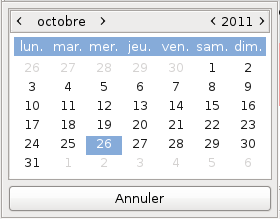
\includegraphics[scale=0.5]{image/screenshot/transactions_calendar}}
	% image entourée par une liste ( picins)
	\fi
	\item les touches \key{+} ou \key{-}, de même que \key{Flèche Gauche} ou \key{Flèche Droite}, permettent de passer au jour précédent ou suivant ;
	\item les touches \key{Flèche Haut} ou \key{Flèche Bas} permettent de passer à la semaine précédente ou suivante ;
	\item les touches \key{Page Haut} ou \key{Page Bas} permettent de passer au mois précédent ou suivant ;
	\item les touches \key{Début} ou \key{Fin} permettent de passer au premier jour ou au dernier jour du mois.
	\item un clic sur le bouton \menu{Annuler} ou l'appui sur la touche \key{Échap} ferme le calendrier sans modifier la date ;
	\item un double-clic ou l'appui sur la touche \key{Entrée} valide la date sélectionnée.
\end{itemize}

\ifIllustration
% espace après image entourée
\vspacehevea{3mm}
\else
\fi


\subsection{Listes déroulantes\label{transactions-new-lists}}

Certains champs disposent d'une liste déroulante de choix déjà définis. Vous pouvez y sélectionner un libellé avec la souris, ou préférer saisir les données au clavier dans le champ de saisie.

L'ouverture d'une liste déroulante peut se faire avec la souris en cliquant sur le petit triangle à droite du champ, ou avec les touches du clavier \key{Page Bas} ou \key{Flèche bas}, le déplacement dans cette liste peut se faire avec la souris, ou avec les touches \key{Page Haut}, \key{Page Bas}, \key{Flèche haut} ou \key{Flèche bas}, et la validation d'un choix à l'intérieur d'une liste déroulante se fait avec la touche \key{Entrée}.

\textbf{Note} : ces triangles peuvent être remplacés, en fonction du thème de l'environnement de bureau ou du gestionnaire de fenêtres que vous utilisez, par d'autres caractères tels que +, -, >, <, etc.

%espace pour changement de thème
\vspacepdf{5mm}
Grisbi vous proposera de compléter automatiquement le mot saisi dès qu'il en aura reconnu suffisamment de caractères. L'\indexword{auto-complètement}\index{champ de saisie !auto-complètement} apparaît sur fond bleu{\couleur}. Pour accepter celui proposé, appuyez sur la touche \key{Tabulation} ou la touche \key{Entrée}, selon votre choix de configuration, sinon continuez la saisie.

Les listes déroulantes des devises, exercices et modes de règlement s'ouvrent avec la touche \key{Espace} ; on s'y déplace  avec les touches \key{Flèche Haut} et \key{Flèche Bas} et l'on  valide avec la touche \key{Espace}.


\subsection{Saisie de formules\label{transactions-new-numbers}}

Dans le formulaire de saisie, vous pouvez saisir les nombres, avec ou sans décimales, dans les champs tels que \menu{Débit} et \menu{Crédit}, à l'aide du clavier.

Vous pouvez aussi y saisir des \indexword{formules arithmétiques}\index{champ de saisie !formule arithmétique}\index{formule arithmétique !champ de saisie} simples, à l'aide des quatre opérateurs d'addition, soustraction, multiplication et division. Cela remplace la \indexword{calculatrice}\index{calculatrice} sur votre bureau.

Pour saisir une formule, saisissez-la comme si c'était un texte, par exemple \og 3,40-2,10\fg{} , puis continuez normalement la saisie des autres champs de votre opération ; si elle est mal écrite, elle s'affiche sur fond rouge{\couleur}. Lorsque vous la validez, le résultat \og 1,30 \fg{} s'affiche dans le champ de saisie, et si la formule est toujours mal écrite, le message \og \#\#\#ERR\#\#\# \fg{} s'affiche à la place et sur fond rouge{\couleur}.

Cette calculatrice accepte la multiplication ou la division, mais de manière exclusive de l'addition ou de la soustraction ; c'est-à-dire qu'on peut mélanger additions et soustractions dans une saisie mais pas une multiplication (ou une division) et un quelconque autre opérateur : on ne peut pas mettre de parenthèses pour indiquer un ordre de priorité d'opération.

Cette fonctionnalité peut être très utile, notamment pour réajuster les montants d'une opération ventilée en cas d'écart. 


\subsection{Remise de chèques ou d'espèces\label{transactions-new-cheque}}

Pour enregistrer une \indexword{remise de chèques}\index{remise !chèques}, vous les déposez d'abord sur votre compte bancaire à la banque qui vous remet un bordereau de remise, puis vous saisissez l'opération de remise, en crédit sur votre compte bancaire.

Pour enregistrer une \indexword{remise d'espèces}\index{remise !espèces}, vous les déposez d'abord soit sur votre compte bancaire à la banque qui vous remet un bordereau de remise, soit dans votre porte-monnaie, puis vous saisissez l'opération de remise, en crédit sur votre compte de caisse.  

% espace pour changement de thème
\vspacepdf{5mm}
Si vous recevez beaucoup de chèques (par exemple parce que vous gérez une association et que vos adhérents payent leur cotisation par chèque), vous avez deux méthodes de gestion :

\begin{itemize}
	\item soit  vous enregistrez individuellement une opération pour chaque chèque dans votre compte bancaire, puis vous groupez ces chèques pour les déposer à la banque ; votre bordereau de remise ne contient alors que leur montant global ; lors du rapprochement bancaire, votre relevé bancaire ne mentionne que ce montant global, mais non le montant de chaque chèque saisi dans votre compte bancaire ; de ce fait, le pointage est rendu peu facile (vous devriez au moins avoir fait auparavant une liste de ces chèques) ;
	\item soit vous enregistrez une seule opération pour tous vos chèques, vous aurez alors perdu l'information du tiers de chaque chèque, et cette information n'apparaîtra pas dans l'onglet \menu{Tiers}, même si vous essayez de ventiler cette opération.
\end{itemize} 

% espace pour changement de thème
\vspacepdf{5mm}
Si aucune de ces méthodes ne vous convient, une meilleure solution consiste à utiliser un \emph{compte d'attente}. Pour cela, la méthode est explicitée en détails au paragraphe \vref{accounts-type-bank-waiting-remittance}, \menu{Remise de chèques ou d'espèces}. 


\subsection{Virements\label{transactions-new-transfer}}


Le terme \indexword{virement}\index{opération !virement} recouvre deux notions différentes : les virements externes et les virements internes. Voici dans chaque cas les méthodes de saisie conseillées.

\subsubsection{Virements externes\label{transactions-new-transfer-external}}

Les \indexword{virements externes}\index{virement !externe} sont des virements que votre banque, ou vous-même si vous passez un ordre par Internet, effectue vers ou à partir de votre compte. Ils peuvent être entrants (par ex. si votre employeur donne l'ordre à votre banque de vous virer le montant de votre salaire) ou sortants (par ex. si vous donnez l'ordre à votre banque de faire un virement Swift pour payer une facture à l'étranger).

Il s'agit d'un type d'opération assimilable à un chèque, et vous pourrez la saisir en sélectionnant le \menu{Moyen de paiement} : \menu{Virement} dans le formulaire de saisie.


\subsubsection{Virements internes\label{transactions-new-transfer-internal}}

Les \indexword{virements internes}\index{virement !interne} sont des transferts entre vos différents comptes de Grisbi, et qui n'ont pas forcément d'équivalent en banque ; voici quelques exemples :

\begin{itemize}
	\item si vous utilisez un compte de caisse, lorsque vous faites un retrait d'espèces à la banque, vous saisissez dans Grisbi un virement vers ce compte de caisse, mais le type d'opération est \menu{Retrait} ;
	\item si vous utilisez un compte d'avances, lorsque vous établissez ou recevez un chèque de remboursement, vous saisissez un virement interne, bien que le type d'opération soit \menu{Chèque} ;
	\item si vous utilisez un compte de passif pour gérer un emprunt, vous saisissez le prélèvement mensuel effectué par votre banque comme un virement interne de votre compte bancaire vers votre compte de passif, en tant que type \menu{Prélèvement} ;
	\item si vous utilisez un compte bancaire pour une carte bancaire à débit différé, vous saisissez le prélèvement mensuel par votre banque comme un virement de votre compte courant vers ce compte de carte.
\end{itemize}

Par contre, si vous n'utilisez aucun de ces comptes et que votre fichier de comptes contient uniquement un compte courant et un compte d'épargne, alors les virements internes correspondent à des virements d'un compte vers l'autre. Ce seront bien des opérations de type \menu{Virement}, et vous les enregistrerez dans la catégorie \menu{Virement : Compte d'épargne} ou \menu{Virement : Compte courant}, selon le cas. 

Vous pouvez réaliser des virements entre comptes en sélectionnant la catégorie \emph{Virement : le\_compte\_ à\_virer}. Selon que vous saisissez son montant en \menu{Débit} ou en \menu{Crédit}, ce sera un virement \emph{vers le compte} ou un virement \emph{à partir du compte}. Il est bien sûr nécessaire que les deux comptes se trouvent dans le même fichier de comptes.

% espace pour changement de thème
\vspacepdf{5mm}
Si vous faites un \indexword{virement entre deux comptes de devises différentes}\index{devise !différente}\index{devise !virement}\index{virement !devise}, Grisbi effectuera automatiquement la conversion, et le débit et le crédit feront apparaître clairement les devises ; par exemple, si vous faites un virement d'un compte en euros vers un compte en yens, dans le compte en yens le virement apparaîtra en yens dans le champ \menu{Crédit}, et son solde en yens sera correct, et dans le compte en euros le débit apparaîtra en yens dans le champ \menu{Débit} et en euros dans le champ \menu{Montant}.

\textbf{Note} : pour que le champ \menu{Montant} s'affiche, vous devrez configurer la liste des opérations et ajuster le nombre de lignes affichées dans la liste des opérations (voir la section \vref{setup-operations-cells}, \menu{Cellules de la liste des opérations} ou la section \vref{transactions-list-fields-manage}, \menu{Gestion des champs d'information}).


\subsubsection{Contre-opération d'un virement\label{transactions-new-transfer-associatedOperation}}

Lorsque vous saisissez une opération de type virement interne, d'un compte vers un autre, ou sur un compte à partir d'un autre, Grisbi crée automatiquement la  \indexword{contre-opération}\index{contre-opération}\index{opération !contre-opération}\index{virement !contre-opération} dans l'autre compte, c'est-à-dire le virement correspondant dans le compte destinataire ou dans le compte origine.

S'il s'agit d'un virement en devises, il créera aussi la contre-opération dans la devise du compte de destination de façon automatique si le taux de change de la devise est fixe, sinon il vous le demandera avant de passer l'écriture.  

% espace pour changement de thème
\vspacepdf{5mm}
Pour \indexword{afficher la contre-opération}\index{contre-opération !afficher} d'un virement, cliquez-droit sur sa ligne dans un des deux comptes, et dans le menu contextuel, sélectionnez \menu{Afficher la contre-opération} : l'autre compte s'affiche et l'opération est sélectionnée (sur fond rouge{\couleur}). Si vous refaites exactement la même manipulation dans ce même compte, le compte d'origine et son virement se réaffichent.


\subsection{Avances : consentement et réception\label{transactions-new-advance}}

Vous pouvez être amené à \indexword{consentir ou recevoir une avance}\index{avance !consentement}\index{avance !réception} de fonds  : il peut s'agir, par exemple, d'une avance sur votre salaire ou d'un achat que vous faites pour le compte d'un de vos amis. 

%espace pour changement de thème
\vspacepdf{5mm}
Vous pouvez gérer cela de deux manières : la plus simple est de créer une catégorie dédiée, et d'y affecter les opérations de débit et de crédit ; quand toutes les avances sont remboursées, le solde de cette catégorie, affiché dans la liste des catégories, doit être égal à zéro (voir la section \vref{categories-list}, \menu{Liste des catégories et des sous-catégories}). Une manière plus intéressante est de créer un compte d'avances, qui permet une vision plus immédiate de l'état des avances en cours : elle est décrite en détails dans le paragraphe \vref{accounts-type-bank-advance}, \menu{Compte d'avances}.


\subsection{Rappel automatique d'une opération\label{transactions-new-recall}}

Le \indexword{rappel automatique}\index{opération !rappel automatique} d'une opération vous permet de saisir beaucoup plus rapidement une opération affectée à un tiers déjà connu par votre fichier de comptes : lors de la saisie du tiers, dès que vous sortez de la zone de saisie, les autres champs du formulaire sont automatiquement complétés à l'identique de la dernière opération saisie pour ce tiers. À vous de les modifier si nécessaire avant de valider l'opération.  

Vous pouvez ajuster finement ce comportement dans le menu \menu{Édition - Préférences} (voir la section \vref{setup-form-input}, \menu{Aide à la saisie du formulaire}).

% espace avant Attention ou Note  : 5 mm
\vspacepdf{5mm}
\textbf{Note} : si vous ne modifiez aucun champ et que vous validez l'opération, vous obtiendrez une opération purement et simplement dupliquée, mais qui portera la date du jour courant.


\section{Saisie d'une opération en devises\label{transactions-currencies}}


Grisbi peut gérer des opérations saisies avec une \indexword{devise différente}\index{devise !différente} de celle du compte, avec ou sans frais de change.

% espace pour changement de thème
\vspacepdf{5mm}
Pour utiliser une devise différente, vous devez d'abord procéder aux configurations suivantes :
\begin{enumerate}
	 \item créez la devise, si elle ne l'est pas déjà, dans le menu \menu{Édition - Préférences} (voir la section \vref{setup-resources-currencies}, \menu{Devises}) ;
	 \item dans le même menu, créez le ou les liens dont vous avez besoin entre la nouvelle devise et les autres déjà enregistrées (voir la section \vref{setup-resources-rate}, \menu{Liens entre devises}) ;
	 \item configurez l'affichage du champ \menu{Devise} dans le formulaire de saisie des opérations (voir la section \vref{setup-form-content}, \menu{Contenu}) ;
	 % saut de ligne pour alignement de la note sur l'item
	 
	 \textbf{Note} : les champs \menu{Devise} et \menu{Change} sont liés dans le formulaire de saisie : la configuration de l'affichage du champ \menu{Devise} dans le formulaire y positionne automatiquement le champ \menu{Change}, et inversement ; vous pouvez ensuite les déplacer dans les cellules voulues.
	 \item configurez l'affichage du champ \menu{Montant} dans la liste des opérations (voir la section \vref{setup-operations-cells}, \menu{Cellules de la liste des opérations} ou la section \vref{transactions-list-fields-manage}, \menu{Gestion des champs d'information}).
\end{enumerate}

% espace pour changement de thème
\vspacepdf{5mm}
Lors de la saisie de l'\indexword{opération en devise}\index{opération !en devise}\index{devise !opération} dans le formulaire de saisie, choisissez dans la liste déroulante la devise dans laquelle l'opération doit être enregistrée. Plusieurs questions peuvent \ifIllustration se poser\refimage{transactions-changeRate-img} :
\else se poser :
\fi

\ifIllustration
% image centrée 
\begin{figure}[htbp]
\begin{center}
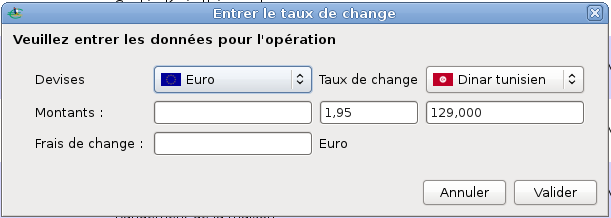
\includegraphics[scale=0.5]{image/screenshot/transactions_changeRate}
\end{center}
\caption{Frais et taux de change}
\label{transactions-changeRate-img}
\end{figure}
% image centrée 
\fi

\begin{itemize}
	 \item si vous n'avez pas créé de lien (taux de change) pour cette devise, Grisbi affiche la fenêtre de  \ifIllustration frais et taux de change \refimage{transactions-changeRate-img} :
	 \else frais et taux de change :
	 \fi
	  saisissez-y le taux de change, validez la fenêtre puis validez l'opération : le montant en devise s'affiche dans le champ \menu{Débit} et celui dans la devise du compte dans le champ \menu{Montant} ;
	  % espace pour notte alignée avec l'item
	  
	  \textbf{Note} : vous pouvez inverser le sens de la conversion (un euro vaut X Devise, ou bien une Devise vaut Y euros) en inversant le nom des devises dans les deux listes déroulantes ; vous pouvez ainsi entrer exactement le taux de change tel qu'il vous est communiqué ; ce taux peut être ajusté à tout moment après la création de l'opération.
	 \item si vous voulez modifier le taux de change, ouvrez l'opération en modification, cliquez sur le bouton \menu{Change} dans le formulaire de saisie, cochez la case de libellé \menu{Modifier le taux de change} si elle ne l'est pas, puis modifiez-le, et validez la fenêtre puis l'opération ;
	 \item si vous avez des \indexword{frais de change}\index{frais de change}, ouvrez l'opération en modification, cliquez sur le bouton \menu{Change} dans le formulaire de saisie, saisissez les frais en devise du compte dans le champ \menu{Frais de change}, et validez la fenêtre puis l'opération ; ces frais sont alors ajoutés au contenu du champ \menu{Montant} ; mais vous pouvez à la place les saisir dans une opération indépendante, en utilisant une catégorie dédiée, par exemple \emph{Frais financiers : Frais bancaires} : cela peut vous permettre de les comptabiliser à part ;
	 \item si vous voulez que le taux de change soit fixe : voir la section \vref{setup-resources-rate}, \menu{Liens entre devises}.
\end{itemize}


\section{Saisie d'une opération avec tiers virtuel\label{transactions-virtualThird}}


Grisbi vous permet d'utiliser des tiers virtuels : un tiers virtuel est un \emph{état} qui représente une liste de plusieurs tiers.

Lorsque vous saisissez une opération avec pour tiers un tiers virtuel, Grisbi enregistre, au moment de sa validation, une opération identique (montant, catégorie, imputation budgétaire, moyen de paiement etc.) pour \emph{chacun} des tiers représentés par ce tiers virtuel. Par exemple, vous pouvez saisir en une seule fois un appel à cotisation pour 200 adhérents d'une association, ce qui représente un gain de temps très appréciable\ldots

% espace pour changement de thème
\vspacepdf{5mm}
Pour \indexword{saisir une opération avec un tiers virtuel}\index{tiers virtuel !saisie d'opération}, saisissez ce tiers  dans le champ \menu{Tiers} du formulaire de saisie, sous la forme \og État : nom\_du\_tiers\_virtuel\fg{}. 

% espace pour changement de thème
\vspacepdf{5mm}
Pour créer un tiers virtuel, créez un état contenant une liste de tiers : voir le paragraphe \vref{reportscreation-display-general-virtualThird}, \menu{Tiers virtuel}.

% espace pour changement de thème
\vspacepdf{5mm}
Pour modifier un tiers virtuel, modifiez l'état qui l'a créé : voir la section \vref{reports-modify}, \menu{Modification d'un état}.

%espace pour changement de thème
\vspacepdf{5mm}
Pour supprimer un tiers virtuel, vous avez deux possibilités :

\begin{itemize}
	\item décochez la case \menu{Considérer les tiers de ce rapport comme un tiers virtuel} dans l'état qui le définit, puis validez (voir la section \vref{reports-modify}, \menu{Modification d'un état}) ;
	\item supprimez l'état qui le définit (voir la section \vref{reports-delete}, \menu{Suppression d'un état}).
\end{itemize}

\ifIllustration
% saut de page pour titre solidaire
\newpage
\fi


\section{Ventilation d'une opération\label{transactions-breakdown}}


\indexword{Ventiler une opération}\index{ventiler !opération} signifie répartir son montant entre plusieurs lignes (par exemple, vos achats au supermarché peuvent se répartir entre les catégories \emph{Alimentation} et \emph{Soins : Habillement}). Vous pouvez aussi répartir une somme sur la même catégorie, mais avec des informations différentes dans le champ \menu{Remarques} (par exemple pour mémoriser le détail d'une opération).


\subsection{Saisie de l'opération ventilée\label{transactions-breakdown-master}}

Pour \indexword{saisir une opération ventilée}\index{opération !ventilée}, procédez comme suit :
	 
\begin{enumerate}
	 \item dans le formulaire, commencez la saisie de votre opération comme une opération normale jusqu'au champ \menu{Catégories}, où vous choisissez la catégorie \menu{Opération ventilée} (vers la fin du menu déroulant, mais il est plus simple de taper \og O \fg{}) ;
	 \item continuez à saisir les autres données, puis validez :
	 \item dans la liste des opérations, apparaissent la première ligne de la nouvelle opération en caractères rouges sur fond bleu{\couleur}, et en-dessous une nouvelle ligne, sur fond rouge{\couleur} donc sélectionnée, avec un total égal à zéro et un  écart égal à la différence entre ce total et la valeur totale de l'opération ventilée, donc \ifIllustration en négatif\refimage{transactions-breakdown-img} ;
	\else en négatif ;
	\fi
	
	\ifIllustration
	% image centrée 
	\begin{figure}[htbp]
	\begin{center}
	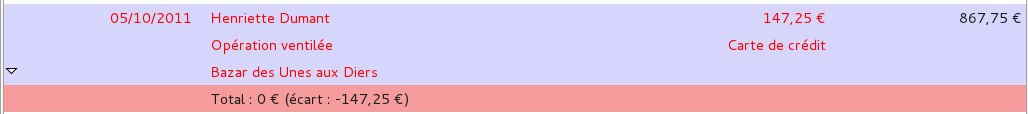
\includegraphics[scale=0.5]{image/screenshot/transactions_breakdown}
	\end{center}
	\caption{Saisie de l'opération ventilée}
	\label{transactions-breakdown-img}
	\end{figure}
	% image centrée 
	\fi

	 \item dans le formulaire, le curseur est dans le champ \menu{Débit}, et les champs  \menu{Date}, \menu{Tiers} et \menu{Moyen de paiement} sont grisés, ce qui signifie qu'on ne peut plus les modifier : il s'agit du formulaire de sous-opération, qui est prêt pour la saisie des sous-opérations ;
	 \item passez à la sous-section suivante \menu{Saisie des sous-opérations ventilées}.
\end{enumerate}


\subsection{Saisie des sous-opérations ventilées\label{transactions-breakdown-slave}}

Pour saisir les \indexword{sous-opérations ventilées}\index{sous-opération !ventilée}, continuez la saisie comme suit :

\textbf{Note} : le montant d'une sous-opération peut-être le résultat d'une opération portant sur plusieurs achats ou dépenses inscrites sur un ticket de caisse ou une facture ; vous pouvez donc utiliser la \indexword{calculatrice}\index{calculatrice} dans les champs de saisie \menu{Débit} ou \menu{Crédit} pour obtenir plus facilement les montants des sous-opérations (voir la section \vref{transactions-new-numbers}, \menu{Saisie de formules}).

\begin{enumerate}
	 \item dans ce formulaire de sous-opération, saisissez les champs libres (non grisés), puis validez votre première sous-opération ;
	 \item dans la liste des opérations, cette sous-opération s'affiche sur fond rose{\couleur}, et une nouvelle ligne apparaît, sur fond rouge{\couleur} donc sélectionnée, qui affiche un total égal à la première sous-opération saisie, en négatif, et un écart égal à la différence entre la valeur totale de l'opération ventilée et la valeur de cette sous-opération, \ifIllustration en négatif\refimage{transactions-breakdown-sub1-img} ;
	\else en négatif ;
	\fi
	
	\ifIllustration
	% image centrée 
	\begin{figure}[htp]
	\begin{center}
	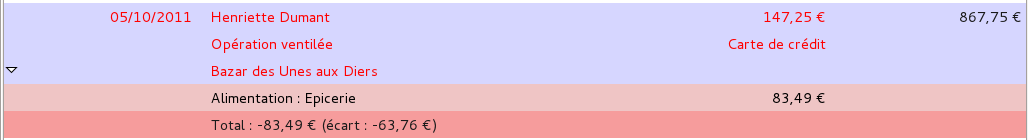
\includegraphics[scale=0.5]{image/screenshot/transactions_breakdown_sub1}
	\end{center}
	\caption{Saisie de la première sous-opération ventilée}
	\label{transactions-breakdown-sub1-img}
	\end{figure}
	% image centrée 
	\fi

	 \item il y a au moins deux sous-opérations dans une opération ventilée (sinon cela n'a aucun intérêt\ldots) ; donc, dans le formulaire de sous-opération, saisissez une deuxième sous-opération de la même manière, puis validez : cette sous-opération s'affiche sur fond rose{\couleur} et une nouvelle ligne apparaît, sur fond rouge{\couleur} donc sélectionnée, qui affiche le dernier total des sous-opérations saisies et le \ifIllustration dernier écart \refimage{transactions-breakdown-sub2-img} ;
	\else dernier écart ;
	\fi
	le total des sous-opérations a augmenté (en négatif) du montant de cette deuxième sous-opération, tandis que l'écart a diminué (en négatif) du même montant ; 

	\ifIllustration
	% image centrée 
	\begin{figure}[htp]
	\begin{center}
	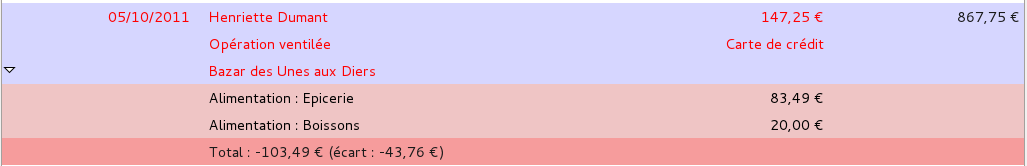
\includegraphics[scale=0.5]{image/screenshot/transactions_breakdown_sub2}
	\end{center}
	\caption{Saisie de la deuxième sous-opération ventilée}
	\label{transactions-breakdown-sub2-img}
	\end{figure}
	% image centrée 
	\fi

	 \item  si l'écart n'est pas nul, on peut alors saisir une troisième sous-opération de la \ifIllustration même manière\refimage{transactions-breakdown-sub3-img},
	\else même manière,
	\fi
	\ifIllustration
	% image centrée 
	\begin{figure}[htp]
	\begin{center}
	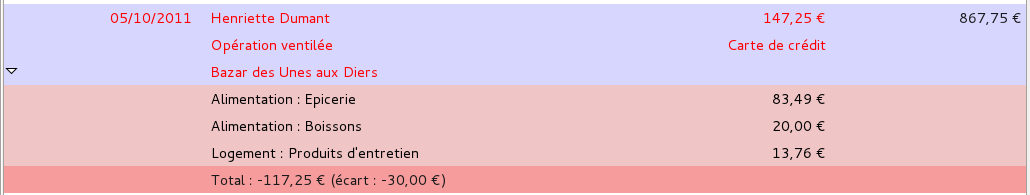
\includegraphics[scale=0.5]{image/screenshot/transactions_breakdown_sub3}
	\end{center}
	\caption{Saisie de la troisième sous-opération ventilée}
	\label{transactions-breakdown-sub3-img}
	\end{figure}
	% image centrée 
	\fi
	et ainsi de suite jusqu'à ce que le montant de votre dernière sous-opération soit exactement égal à l'écart affiché ; validez celle-ci : la dernière sous-opération s'affiche sur fond rose{\couleur} et une nouvelle ligne sur fond rose{\couleur} apparaît, vide, ce qui indique qu'il n'y a plus d'écart et que la somme des sous-opérations est bien égale à la valeur totale de l'opération \ifIllustration  ventilée\refimage{transactions-breakdown-complete-img}.
	\else ventilée.
	\fi
	
	\ifIllustration
	% image centrée 
	\begin{figure}[htp]
	\begin{center}
	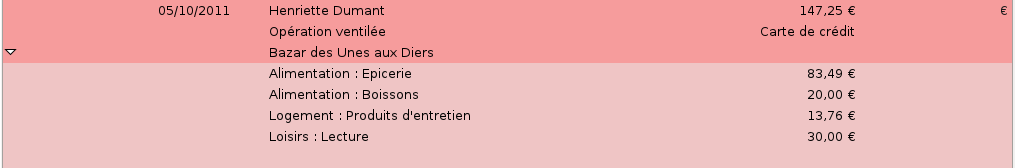
\includegraphics[scale=0.5]{image/screenshot/transactions_breakdown_complete}
	\end{center}
	\caption{Saisie de la dernière sous-opération ventilée}
	\label{transactions-breakdown-complete-img}
	\end{figure}
	% image centrée 
	\fi
	 
		 \item passez à la sous-section suivante \menu{Validation de l'opération ventilée}.
\end{enumerate}


\subsection{Validation de l'opération ventilée\label{transactions-breakdown-validation}}

À ce moment, toutes les sous-opérations sont entrées et validées et, dans la liste des opérations, la ligne de l'opération ventilée est affichée sur fond rouge{\couleur}, donc sélectionnée. Le formulaire réaffiche les données que vous y avez saisies. Toutes les sous-opérations étant correctes, validez l'opération ventilée, qui s'affiche alors dans la liste des opérations, en caractères noirs et sur fond rouge{\couleur}, sans les \ifIllustration sous-opérations\refimage{transactions-breakdown-oneLine-img}.
\else sous-opérations.
\fi

\ifIllustration
% image centrée 
\begin{figure}[htp]
\begin{center}

\includegraphics[scale=0.5]{image/screenshot/transactions_breakdown_oneLine}
\end{center}
\caption{Opération ventilée validée}
\label{transactions-breakdown-oneLine-img}
\end{figure}
% image centrée 
\fi

Une fois le dernier champ du formulaire saisi et validé, la ligne active, en rouge{\couleur}, passe à la dernière ligne vide de la liste, comme pour une opération normale.

Vous pouvez vérifier tout le contenu de cette opération ventilée, en cliquant sur le petit triangle à gauche de sa ligne pour dérouler \ifIllustration l'opération\refimage{transactions-breakdown-complete-img}. 
\else l'opération.
\fi

\textbf{Note} : ces triangles peuvent être remplacés, en fonction du thème de l'environnement de bureau ou du gestionnaire de fenêtres que vous utilisez, par d'autres caractères tels que +, -, >, <, etc.

% espace après Attention ou Note : 5 mm
\vspacepdf{5mm}
Vous pouvez alors modifier les sous-opérations en les sélectionnant et en modifiant leurs champs de la même manière, et de façon à ce que finalement leur somme soit égale à la valeur de l'opération ventilée.


\subsection{Rappel automatique d'une opération ventilée\label{transactions-breakdown-recall}}

Le \indexword{rappel automatique}\index{opération !rappel automatique} d'une opération ventilée 
fonctionne comme celui d'une opération normale (voir la section \vref{transactions-new-recall}, \menu{Rappel automatique d'une opération}). 

Cependant, pour une opération ventilée, un champ supplémentaire \menu{Restaurer les sous-opérations} apparaît en bas du formulaire de saisie, à gauche des boutons \menu{Annuler} et \menu{Valider}, et vous pouvez cocher la case correspondante en cliquant dessus ou sur le champ, et selon votre besoin.


\section{Modification d'une opération\label{transactions-modify}}


Pour modifier une opération ou une sous-opération ventilée, sélectionnez-la pour qu'elle s'affiche dans le formulaire de saisie, puis passez en mode édition par l'une de ces méthodes :

\begin{itemize}
	 \item appuyez sur la touche du clavier \key{Entrée} ;
	 \item dans la barre de menus, sélectionnez \menu{Édition - Éditer l'opération} ;
	 \item dans la barre d'outils, cliquez sur \menu{Éditer} ;
	 \item dans le menu contextuel, sélectionnez \menu{Éditer l'opération} ;
	 \item dans l'un des champs du formulaire, cliquez-gauche.
\end{itemize}
 
Si le formulaire de saisie n'était pas affiché, il s'affiche. La date s'affiche sur fond bleu{\couleur} dans le formulaire.

Il est alors possible de modifier toutes les informations désirées, en se déplaçant dans les champs de saisie. 

La combinaison de touches \key{Ctrl} \key{P} donne ou retire à une opération sélectionnée le statut d'\indexword{opération pointée}\index{opération !pointée}, et \key{Ctrl} \key{R} celui d'\indexword{opération rapprochée}\index{opération !rapprochée} (voir le chapitre \vref{reconciliation}, \menu{Rapprochement bancaire}). Vous pouvez aussi donner à une opération le statut d'opération pointée, mais uniquement celui-ci, par la combinaison \key{Ctrl} \key{Clic} dans la colonne P/R, sur la ligne de l'opération à pointer.

% espace pour changement de thème
\vspacepdf{5mm}
Si l'opération a déjà été rapprochée (voir le chapitre \vref{reconciliation}, \menu{Rapprochement bancaire}), il est par contre impossible de modifier son montant. Les autres champs restent modifiables. Si vous avez vraiment et impérativement besoin de modifier le montant (mais si vous avez déjà rapproché l'opération, cela ne devrait pas être le cas), procédez comme suit :

\begin{enumerate}
	 \item sélectionnez l'opération ;
	 \item annulez son statut \emph{Rapproché} en appuyant sur la combinaison de touches \key{Ctrl} \key{R} ;
	 \item modifiez l'opération ;
	 \item appuyez à nouveau sur la combinaison de touches \key{Ctrl} \key{R}. Si vous ne le faisiez pas, le rapprochement relatif à cette opération serait faussé, d'une valeur égale à la différence entre le précédent et le nouveau montant de cette opération.
\end{enumerate}

\strong{Attention} : cette manipulation est hautement déconseillée, car elle fausse momentanément le rapprochement associé à cette opération, et il redevient exact à la fin, si vous n'en avez pas modifié le montant (cette manipulation sera d'ailleurs probablement automatiquement désactivée dans une future version de Grisbi dans le cas d'une comptabilité de type association).


\section{Suppression d'une opération\label{transactions-delete}}


Pour supprimer une opération, sélectionnez-la, et utilisez l'une de ces
méthodes :
\begin{itemize}
	 \item appuyez sur la touche du clavier \key{Suppr} ;
	 \item dans la barre de menus, sélectionnez \menu{Édition - Supprimer une opération} ;
	 \item dans la barre d'outils, cliquez-gauche sur \menu{Supprimer} ;
	 \item dans le menu contextuel, sélectionnez \menu{Supprimer l'opération}.
\end{itemize}

% espace pour changement de thème
\vspacepdf{5mm}
La suppression d'une sous-opération ventilée se fait de la même façon, mais vous devrez faire en sorte que finalement la somme des sous-opérations soit égale à la valeur de l'opération ventilée.

\ifIllustration
% espace pour changement de thème
\vspacepdf{5mm}
\fi

La suppression n'est pas possible si :

\begin{itemize}
	 \item l'opération est ouverte en modification : il faut préalablement sortir du mode édition, en utilisant la touche \key{Échap} ;
	 \item l'opération est \indexword{rapprochée}\index{opération !rapprochée} (il faut préalablement annuler son statut \emph{Rapproché} en appuyant sur la combinaison de touches \key{Ctrl} \key{R}).
\end{itemize}

% espace avant Attention ou Note  : 5 mm
\vspacepdf{5mm}
\strong{Attention} : cette dernière manipulation est hautement déconseillée car elle fausse le rapprochement associé à cette opération.


\section{Opération sélectionnée comme modèle\label{transactions-model}}


Pour utiliser une \indexword{opération comme modèle}\index{opération !modèle}, sélectionnez-la, et utilisez l'une de ces méthodes :
\begin{itemize}
	 \item dans la barre de menus, sélectionnez \menu{Édition - Utiliser l'opération sélectionnée comme modèle} ;
	 \item dans le menu contextuel, sélectionnez \menu{Édition - Utiliser l'opération sélectionnée comme modèle}.
\end{itemize}

% espace pour changement de thème
\vspacepdf{5mm}
Une nouvelle opération s'affiche sur fond rouge{\couleur}, dans une nouvelle ligne en-dessous de l'opération sélectionnée précédemment ; elle n'a évidemment ni le statut \emph{Pointé} ni le statut \emph{Rapproché}.

Vous pouvez alors éditer cette nouvelle opération, par exemple en modifiant sa date.


\section{Clonage d'une opération\label{transactions-duplicate}}


Pour cloner une opération, sélectionnez-la pour qu'elle s'affiche dans le formulaire de saisie, puis utilisez l'une de ces deux méthodes :

\begin{itemize}
	 \item dans la barre de menus, sélectionnez \menu{Édition - Cloner l'opération} ;
	 \item dans le menu contextuel, sélectionnez \menu{Cloner l'opération}.
\end{itemize}

% espace pour changement de thème
\vspacepdf{5mm}
L'opération sélectionnée précédemment apparaît toujours sur fond rouge{\couleur}, et l'opération clonée s'affiche dans une nouvelle ligne en-dessous ; elle n'a évidemment ni le statut \emph{Pointé} ni le statut \emph{Rapproché}.

Vous pouvez alors éditer cette nouvelle opération, par exemple en modifiant la date.


\section{Conversion d'une opération en opération planifiée\label{transactions-schedule}}


Pour convertir une opération en opération planifiée, sélectionnez-la pour qu'elle s'affiche dans le formulaire de saisie, puis utilisez l'une de ces deux méthodes :
\begin{itemize}
	 \item dans la barre de menus, sélectionnez \menu{Édition - Convertir en opération planifiée} ;
	 \item dans le menu contextuel, sélectionnez \menu{Convertir l'opération en opération planifiée}.
\end{itemize}

% espace pour changement de thème
\vspacepdf{5mm}
L'onglet \menu{Échéancier} s'affiche. La nouvelle opération apparaît dans la liste des opérations planifiées, et le formulaire de saisie s'affiche avec les paramètres de l'opération. Vérifiez ou éditez ces paramètres selon vos besoins, puis validez.


\section{Déplacement d'une opération vers un autre compte\label{transactions-move}}


Pour déplacer une opération dans un autre compte, sélectionnez-la, puis utilisez l'une de ces deux méthodes :

\begin{itemize}
	 \item dans la barre de menus, sélectionnez \menu{Édition - Déplacer l'opération vers un autre compte} et choisissez le compte destinataire dans la liste ;
	 \item dans le menu contextuel, sélectionnez \menu{Déplacer l'opération vers un autre compte} et choisissez le compte destinataire dans la liste.
\end{itemize}

Il est bien entendu que les deux comptes doivent se trouver dans le même fichier de comptes.

% espace avant Attention ou Note  : 5 mm
\vspacepdf{5mm}
\textbf{Note} : il est impossible de déplacer une opération si elle a le statut \emph{Rapproché}. Par contre, c'est possible si elle a le statut \emph{Pointé}.



\section{Recherche d'un montant ou d'une chaîne de caractères \label{transactions-find}}

Pour rechercher un montant ou une chaîne de caractères, à partir du menu contextuel, sélectionnez \menu{Rechercher} ; une fenêtre de recherche apparaît ; dans le champ \menu{Chaîne recherchée}, entrez la chaîne de caractères voulue, que ce soit un nombre ou du texte, puis :
METTRE DANS L'INDEX

\begin{enumerate}
	\item si vous avez saisi du texte, cliquez sur le bouton \menu{Chaîne recherchée}, puis ;
	\begin{itemize}	
		\item sélectionnez ou non \menu{Chercher dans les tiers} et \menu{Chercher dans les notes} ;
		\item sélectionnez ou non \menu{Ignorer la \indexword{casse}\index{casse}}, pour afficher les majuscules et  les minuscules ;
		\item sélectionnez ou non \menu{Chercher dans les opérations archivées} ;
		\item sélectionnez ou non \menu{Chercher du plus récent au plus ancien}, pour l'ordre d'affichage des occurrences ; 
		\item cliquez sur le bouton \menu{Rechercher} : le nombre d'occurrences trouvées s'affiche en bas de le fenêtre, et la première occurrence apparaît sur fond rose{\couleur} dans la liste des opérations, en fonction de l'ordre choisi ; cliquez sur le bouton \menu{Rechercher} pour afficher chaque occurrence suivante ; quand la dernière a été affichée, la première s'affiche à nouveau ; si le message « Aucune opération trouvée » s'affiche à là place, juste en-dessous le libellé \menu{Continuer avec un autre compte} s'affiche en caractères normaux et vous pouvez utiliser la liste déroulante \menu{Choisissez un autre compte} ;
	\end{itemize}	
	\item si vous avez saisi un montant, il peut être positif (crédit) ou négatif (débit), et dans ce cas il doit être signé (par ex. -17,50), cliquez sur le bouton \menu{Chercher un montant}, puis ;
	\begin{itemize}
		\item si vous ne sélectionnez pas \menu{Chercher un montant à + ou -}, la recherche ne donnera que des nombres strictement exacts à la chaîne recherchée (-17,50 dans notre exemple);
		\item si vous sélectionnez \menu{Chercher un montant à + ou -}, choisissez un écart au montant exact (par exemple 5), en cliquant sur les boutons \menu{+} ou \menu{-}, et la recherche donnera tous les montants se trouvant dans l’intervalle entre -12,50 et -22,50 dans notre exemple ;
		\item sélectionnez ou non \menu{Chercher dans les opérations archivées} ;
		\item sélectionnez ou non \menu{Chercher du plus récent au plus ancien}, pour l'ordre d'affichage des occurrences ; 
		\item cliquez sur le bouton \menu{Rechercher} : le nombre d'occurrences trouvées s'affiche en bas de le fenêtre, et la première occurrence apparaît sur fond rose{\couleur} dans la liste des opérations, en fonction de l'ordre choisi ; cliquez sur le bouton \menu{Rechercher} pour afficher chaque occurrence suivante ; quand la dernière a été affichée, la première s'affiche à nouveau ;	si le message « Aucune opération trouvée » s'affiche à là place, juste en-dessous le libellé \menu{Continuer avec un autre compte} s'affiche en caractères normaux et vous pouvez utiliser la liste déroulante \menu{Choisissez un autre compte}.	
	\end{itemize}	
\end{enumerate}




\section{Nouveau tiers, catégorie ou imputation budgétaire\label{transactions-fillcombo}}


Il peut arriver que vous ayez besoin d'un nouveau tiers, d'une nouvelle catégorie ou d'une nouvelle imputation budgétaire pendant une saisie d'opération. Dans ce cas, Grisbi permet d'en faire la création \og à la volée \fg{} : saisissez le nouveau nom dans la zone de liste déroulante, et Grisbi l'ajoutera automatiquement à la liste. Vous pourrez ultérieurement faire toutes les modifications nécessaires dans les onglets \menu{Tiers} (voir la section \vref{thirdparties-modify}, \menu{Modification d'un tiers}), \menu{Catégories} (voir la section \vref{categories-modify}, \menu{Modification d'une catégorie ou d'une sous-catégorie}) ou \menu{Imputations budgétaires} (voir la section \vref{budgetarylines-modify}, \menu{Modification d'une (sous-) imputation budgétaire}).
 
% espace avant Attention ou Note  : 5 mm
\vspacepdf{5mm} 
\textbf{Note} : pour saisir une \indexword{catégorie}\index{catégories !syntaxe}\index{sous-catégories !syntaxe}\index{syntaxe !catégories : sous-catégories}
 (ou une \indexword{imputation budgétaire} : sous-imputation budgétaire\index{imputations budgétaires !syntaxe}\index{sous-imputations budgétaires !syntaxe}\index{syntaxe !imputations budgétaires : sous-imputations budgétaires}) avec une sous-catégorie (ou sous-imputation), il faut respecter la syntaxe \emph{catégorie : sous-catégorie} (avec les deux points comme séparateur, encadrés par des espaces), sinon Grisbi ne comprendra pas. De même si vous ajoutez une nouvelle sous-catégorie (ou sous-imputation budgétaire) à une catégorie (ou imputation) existante.
% espace après Attention ou Note  : 5 mm
\vspacepdf{5mm}

Vous pouvez également créer un tiers, une catégorie ou une imputation budgétaire directement dans leur onglet respectif, sélectionné dans le panneau de navigation.


\section{Impression de la liste des opérations\label{transactions-print}}


Pour imprimer la liste des opérations, cliquez sur le bouton \menu{Imprimer} de la barre d'outils ; une fenêtre d'impression s'ouvre, dont l'aspect et les fonctions dépendent de votre gestionnaire d'impression ; vous aurez le plus souvent les choix suivants :

\begin{itemize}
	\item imprimer dans un fichier (au format \gls{PostScript}, \gls{PDF} ou \gls{SVG}) ;
	\item imprimer avec votre imprimante.
\end{itemize}

En fonction de votre gestionnaire d'impression, vous pourrez disposer de réglages divers tels que la taille et l'orientation de la feuille, la résolution, la police d'impression et sa taille, etc.

% espace avant Attention ou Note  : 5 mm
\vspacepdf{5mm}
\textbf{Note} : la liste des opérations de certains comptes peut être très longue ; affichez un aperçu avant impression pour vérifier ce que vous allez imprimer.


%XXXXXXXXXXXXXXXXXXXXXXXXXXXXXXXXXXXXXXXXXXXXXXXXXXXXXXXXXXXXXXXXXXXXXXXXXXXXXXXXXX
%
% [benj] supprimé car franchement, ça n'a rien à faire ici.
%
% PLEASE NOTE !  DO NOT TRANSLATE THE FOLLOWING SECTION
%\section{Quelques mots sur un anglicisme trop répandu}
%
%On voit régulièrement dans les documentations, livres et autres articles,
%publiés sur l'Internet et ailleurs, le mot \emph{complétion}. Ceci est un
%horrible anglicisme. 
%
%Que l'on assimile un mot anglais lorsque le mot français équivalent n'existe pas
%peut se comprendre, encore que le néologisme intelligent me semble préférable.
%Il ne s'agit bien sûr pas de tomber dans le ridicule de nos académiciens qui
%traduisent mail par mèl et CD-Rom par cédérom. Passons sur leur manque
%d'imagination alors qu'ils ont su par autrefois créer des mots comme disquette,
%informatique et ordinateur, qui n'existent nulle part ailleurs !
%
%Dans le cas précis du mot \emph{complétion} un traducteur du \emph{Guide de
%l'administration réseau sous linux,} Editions O'Reilly, avait cru bien faire en
%essayant de créer le mot \emph{complétement} (avec un accent aigu) qui voulait
%signifier \emph{action de compléter}. L'initiative était louable mais ô combien
%risquée \ldots En effet lorsque l'on s'essaye à ce genre d'exercice de style, il est
%prudent de maîtriser tous les rouages de la langue. Et en l'occurrence il existe
%une règle dite la \emph{règle de l'ernance} (page 56 du \emph{Bescherelle
%Orthographe}) \footnote{Si quelqu'un possède ce livre je serais très heureux
%qu'il me fasse parvenir le texte exact de cette règle. Je ne l'ai 
%malheureusement plus\ldots} qui explique parfaitement le mécanisme de
%changement d'accent entre un verbe et le substantif dérivé
%\footm{André Cianfarini, qui se définit lui-même comme \emph{un développeur autodidacte qui n'a jamais fini sa thèse de grammaire pour cause de relations passionnelles avec l'informatique} me communique les précisions suivantes : 
%\begin{quote}
%C'est un processus phonologique qui est à l'origine de ces
%transformations ; pour simplifier, on pourrait le résumer ainsi :
%un "e" fermé (l'avant-dernier "e" de "préférer" par exemple) devient un
%"e" ouvert (l'avant-dernier "e" de "je préfère" par exemple) lorsque la
%syllabe qui le suit est atone.
%\end{quote} 
%}. Si ce malheureux
%traducteur l'avait connue il n'aurait pas commis cet affreux barbarisme\ldots
%
%Et si avant toute chose ce traducteur avait eu l'idée de vérifier dans son
%dictionnaire que le mot n'existait pas déjà\ldots il aurait trouvé :
%
%\begin{description}
%
%\item [complètement]n.m. Action de compléter : \emph{le complètement
%d'un livre}. 
%
%\end{description}
%
%Et j'ai bien pris soin de chercher ce mot dans le plus vieil exemplaire du
%\emph{Larousse universel} en ma possession, soit l'édition de 1949 !
%
%Donc adoptons sans aucun remord le mot complètement, et, puisque cette action
%est automatique, allons sans crainte jusqu'à écrire auto-complètement, ce qui
%est parfaitement compréhensible, intuitif et 100\% français !
%
%Cocorico !
%
%Et puissent ces quelques lignes tordre définitivement le cou au mot complétion,
%cette \emph{affreuseté non-permissable} ! ;-)
%
%from now you can translate again
\myclearemptydoublepage

%%%%%%%%%%%%%%%%%%%%%%%%%%%%%%%%%%%%%%%%%%%%%%%%%%%%%%%%%%%%%%%%%
% Contents : The reconciliation chapter
% $Id : grisbi-manuel-reconciliation.tex, v 0.4 2002/10/27 Daniel Cartron
% $Id : grisbi-manuel-reconciliation.tex, v 0.5.0 2004/06/01 Loic Breilloux
% $Id : grisbi-manuel-reconciliation.tex, v 0.6.0 2011/11/17 Jean-Luc Duflot
% $Id : grisbi-manuel-reconciliation.tex, v 0.8.9 2012/04/27 Jean-Luc Duflot
% $Id : grisbi-manuel-reconciliation.tex, v 1.0 2014/02/12 Jean-Luc Duflot
%%%%%%%%%%%%%%%%%%%%%%%%%%%%%%%%%%%%%%%%%%%%%%%%%%%%%%%%%%%%%%%%%

\chapter{Rapprochement bancaire\label{reconciliation}}


Les rapprochements bancaires servent à vérifier la bonne correspondance entre l'historique des opérations dans votre compte bancaire et les opérations saisies dans Grisbi. Faire un rapprochement bancaire consiste donc à faire une comparaison entre un relevé de votre compte  bancaire et les opérations enregistrées dans le compte correspondant dans Grisbi. Un rapprochement dans Grisbi est une représentation d'un relevé bancaire, comprenant un solde initial, des opérations et un solde final. Cette représentation est figée, comme le relevé bancaire. Donc une fois qu'un rapprochement est terminé et est correct, on ne devrait pas avoir à le modifier, sauf dans des cas exceptionnels.

Il est conseillé de faire les rapprochements de vos comptes régulièrement : cela permet aussi de détecter, autant dans Grisbi que dans votre relevé bancaire, des oublis ou des erreurs de saisie d'opérations, des décalages de tirage d'opérations, l'existence de frais bancaires, etc.


\section{Rapprochement d'un compte\label{reconciliation-account}}


Pour faire un rapprochement bancaire, munissez-vous du relevé de votre compte bancaire, et affichez la liste des opérations du compte correspondant sur Grisbi (voir le chapitre \vref{transactions}, \menu{Opérations d'un compte}).


\subsection{Description\label{reconciliation-account-description}}

Pour avoir accès à la fonction de rapprochement bancaire, cliquez sur \menu{Rapprocher} dans la barre \ifIllustration d'outils\refimage{reconciliation-list-img}.
\else d'outils.
\fi

\ifIllustration
% image centrée
\begin{figure}[htbp]
\begin{center}
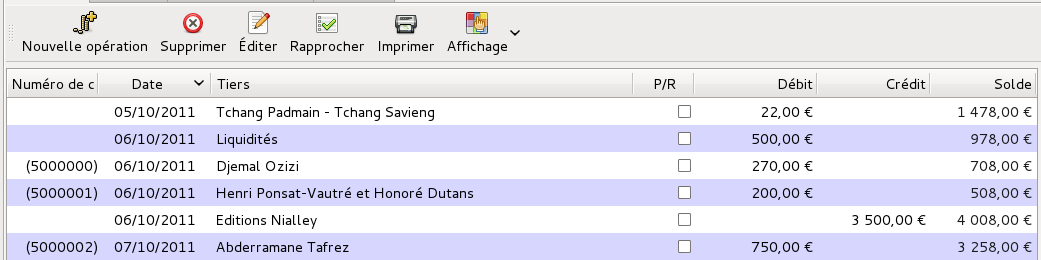
\includegraphics[scale=0.5]{image/screenshot/reconciliation_list}
\end{center}
\caption{Liste des opérations pendant un rapprochement}
\label{reconciliation-list-img}
\end{figure}
% image centrée
\fi

Les opérations s'affichent alors en mode \menu{Vue simple} (une seule ligne)\ifIllustration \refimage{reconciliation-list-img}, et la zone de rapprochement apparaît à gauche, en-dessous du panneau de navigation.
\else , et la zone de rapprochement apparaît à gauche, en-dessous du panneau de navigation.
\fi

L'affichage et le fonctionnement de la liste d'opérations se comportent de la même manière qu'en dehors de la fonction de rapprochement, en résumé : largeur et libellé des colonnes, déplacement de la liste, \indexword{affichage des opérations}\index{affichage !opérations}, menu contextuel, affichage des champs, \indexword{\glspl{tri}} des opérations\index{tri !opérations}.

Vous pouvez donc exécuter sur cette liste les mêmes actions qu'en dehors de la fonction de rapprochement, que ce soit au moyen de la barre d'outils ou du menu contextuel : sélection, création, ventilation, modification, suppression, etc. Reportez vous pour cela au chapitre \vref{transactions}, \menu{Opérations d'un compte}.

%espace pour changement de thème
\vspacepdf{5mm}

La zone de rapprochement comporte plusieurs éléments :
% espace avant image 5mm
\vspacepdf{3mm}

% Pas de référence à l'illustration car erreur de numéro de figure avec picins.
\begin{itemize}
	\ifIllustration
	% image entourée par une liste (picins)
	% supprimé car en html les figures entourées ne sont pas numérotées, et la numérotation des figures centrées décalée par rapport au pdf
	%\piccaption{Zone de rapprochement}
	\label{reconciliation-infos-img}
	\parpic[r]{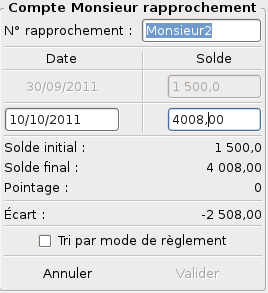
\includegraphics[scale=0.5]{image/screenshot/reconciliation_infos}}
	% image entourée par une liste (picins)
	\fi
	 \item le nom du compte à rapprocher, suivi de \og rapprochement \fg{} ;
	 \item une zone de saisie \menu{\No rapprochement} pour le numéro de rapprochement ;
	 \item un tableau de deux colonnes pour les dates et les soldes, et de deux lignes pour le rapprochement précédent et celui en cours ; seule la deuxième ligne est constituée de champs de saisie ; 
	 \item trois lignes pour le \indexword{solde initial}\index{solde !initial}, le \indexword{solde final}\index{solde !final} et le \indexword{pointage}\index{pointage}, qui est la somme des opérations pointées ;
	 \item une ligne pour l'écart, qui est différent de zéro tant que le total des pointages ne correspond pas à la différence entre le solde initial et le solde final du relevé bancaire ;
	 \item une ligne pour le choix du \gls{tri} par mode de règlement ;
	 \item les boutons \menu{Annuler} et \menu{Valider}.
\end{itemize}

% espace pour changement de thème
\vspacepdf{5mm}

Le \menu{\No rapprochement} est le seul paramètre qui permet d'identifier à coup sûr un rapprochement quelconque ; ce numéro peut comprendre du texte et des nombres. Par défaut, Grisbi attribue un numéro à chaque rapprochement, composé du nom du compte concerné, suivi d'un nombre ; ce nombre est incrémenté automatiquement au rapprochement suivant. Ce \menu{\No rapprochement} est donc unique pour chaque rapprochement d'un compte, et il est visible dans le menu \menu{Préférences - Rapprochement} (voir la section \vref{setup-operations-reconciliation}, \menu{Rapprochement}. 

Grisbi vous permet de personnaliser cette numérotation, qui devra être de la forme \og texte + nombre \fg{}, pour être unique pour chacun de vos rapprochements. Vous pouvez inventer la numérotation qui vous convient, et ce, compte par compte ; par exemple, ils pourront porter le même numéro que vos relevés bancaires. Si, pour quelque raison, le \menu{\No rapprochement} ne respecte pas cette forme, il vous sera difficile de retrouver son contenu, c'est à dire les opérations qui lui appartiennent (voir la section \vref{reconciliation-manage-content}, \menu{Contenu d'un rapprochement}) ; cependant, vous pourrez toujours y modifier le numéro de chaque rapprochement, mais cela risque d'être assez fastidieux \ldots

% espace avant Attention ou Note  : 5 mm
\vspacepdf{5mm}
\textbf{Note} : s'il vous est possible d'avoir la même \indexword{numérotation}\index{rapprochement !numérotation} pour les rapprochements (par ex. de 1 à n) dans des comptes différents, il est impossible de l'avoir plusieurs fois dans un même compte. Vous pourrez par exemple prévoir une numérotation du type année-numéro : 2003-01 pour votre premier relevé mensuel de 2003, et ensuite Grisbi numérotera les suivants jusqu'à 2003-12 ; l'année suivante vous numéroterez le premier 2004-01, etc. Quelque soit le contenu de votre numérotation, il suffit que la fin soit numérique pour que Grisbi sache l'incrémenter, par exemple AV-001 ou REM-001, ou bien encore CCP-1106 pour compte CCP année 2011 mois 06, qui ne permettra aucune confusion sur les comptes et les dates. 
% espace après Attention ou Note  : 5 mm
\vspacepdf{5mm}

Les date et solde du \indexword{rapprochement précédent}\index{rapprochement !précédent} sont automatiquement repris du dernier rapprochement, donc ne sont pas modifiables, et sont en grisé. Mais ce ne sera bien évidemment pas le cas lors du premier rapprochement, où le solde initial est celui que vous avez entré lors de la création du compte (voir la section \vref{accounts-properties}, \menu{Propriétés d'un compte}).

La date du \indexword{rapprochement en cours}\index{rapprochement !en cours} peut être saisie avec le clavier ou le calendrier, disponibles comme dans tout champ de date dans Grisbi (voir les sections \vref{transactions-new-dates}, \menu{Saisie de date au clavier} ou \vref{transactions-new-calendar}, \menu{Saisie de date au calendrier}).

% espace avant Attention ou Note  : 5 mm
\vspacepdf{5mm}
\strong{Attention} : la date finale du rapprochement précédent et la date initiale du rapprochement en cours peuvent être identiques, ou doivent se suivre chronologiquement, pour ne pas avoir de chevauchement de périodes de rapprochement ; cependant, si vous avez fait de telles erreurs, Grisbi pourra probablement les corriger : voir la section \vref{reconciliation-manage}, \menu {Gestion des rapprochements des comptes}.
% espace arès Attention ou Note  : 5 mm
\vspacepdf{5mm}

Afin de faciliter l'identification des opérations pendant le rapprochement vous pouvez toujours changer l'\indexword{ordre d'affichage} des opérations\index{rapprochement !ordre d'affichage}, pour qu'il corresponde à celui de votre relevé bancaire. Ou bien, si vous avez beaucoup d'opérations à rapprocher, vous pouvez par exemple les classer par ordre de montants croissants ou décroissants, pour faciliter la recherche d'un montant ; quand le rapprochement sera terminé, vous rétablirez le classement par date pour avoir un solde juste en fin de liste (voir la section \vref{transactions-list-sorts}, \menu{Tris}).

% espace pour changement de thème : 5 mm
\vspacepdf{5mm}
Vous pouvez aussi trier les opérations en cochant la case \menu{Tri par mode de règlement} dans la zone de rapprochement, ou bien en configurant l'ordre d'affichage selon ces modes de règlement, individuellement pour chaque compte, dans le menu  \menu{Édition - Préférences} (voir la section \vref{setup-operations-sort}, \menu{Option de tri pour les rapprochements}).

% espace pour changement de thème : 5 mm
\vspacepdf{5mm}
Vous pouvez encore masquer ou afficher les \indexword{opérations rapprochées}\index{affichage  !opérations rapprochées} (\og \textbf{R} \fg{}), grâce aux choix proposés par la fonction \menu{Affichage} de la barre de menus ou de la barre d'outils, ou bien, plus simplement, par la combinaison de touches \key{Alt}\key{R}. 

\subsection{Procédure de rapprochement\label{reconciliation-account-howto} }

La procédure pour opérer un rapprochement est la suivante :

\begin{enumerate}
	 \item dans la barre d'outils, cliquez sur \menu{Rapprocher} ;
	 \item vérifiez que la \indexword{zone de rapprochement}\index{rapprochement !zone} affiche un \indexword{numéro de rapprochement}\index{rapprochement !numéro}, sinon saisissez-en un, sous la forme \og texte + nombre \fg{} qui sera unique pour chacun d'eux ; pour les rapprochements suivants, Grisbi incrémentera automatiquement ce nombre ;
	 % saut de ligne pour indentation correcte de la note dans la liste
 
\textbf{Note} : l'incrémentation ne fonctionnera que si la numérotation de votre rapprochement se termine par un chiffre, par exemple \og CCP-201106 \fg{}, et pas du tout dans le cas de \og 201106-CCP \fg{}.
		
	 \item la première ligne du tableau indique la date du rapprochement précédent et le solde à cette date, qui sont alors la date et le solde initiaux de votre rapprochement en cours : ils sont en grisé, vous ne pouvez donc pas les modifier ; ce solde initial est aussi celui de votre dernier relevé bancaire ; il est reporté dans la ligne \menu{\indexword{Solde initial}}\index{solde ! initial} en-dessous ;
	 \item dans la seconde ligne du tableau, saisissez la date du jour (ou celle du relevé bancaire) (voir les sections \vref{transactions-new-dates}, \menu{Saisie de date au clavier} ou \vref{transactions-new-calendar}, \menu{Saisie de date au calendrier}) ainsi que le solde courant, que vous trouvez sur votre dernier relevé bancaire : ce sont la date et le solde de fin de votre rapprochement ; de même, ce solde est reporté dans la ligne \menu{Solde final} en-dessous ;
	 \item dans la liste des opérations, pour chaque opération commune à votre compte et votre relevé bancaires, cochez l'opération dans votre relevé bancaire, et pointez dans Grisbi l'opération par l'un des moyens suivants :
	 
		\begin{itemize}
			\item cliquez sur la ligne d'opération dans la \indexword{colonne} \menu{P/R}\index{colonne !P/R},
			\item appuyez sur la  combinaison de touches \key{Ctrl}\key{P},
			\item appuyez sur la barre d'espace (ce qui déplace aussi la sélection sur la ligne en-dessous) ;			
		\end{itemize}	 
un \og \textbf{P} \fg{} y apparaît alors pour indiquer que l'opération est \og pointée \fg{} ; si vous vous êtes trompé(e), un autre clic, un autre \key{Ctrl}\key{P} ou un autre appui sur la barre d'espace (précédé du déplacement de la sélection sur la ligne au-dessus) supprime le \og \textbf{P} \fg{} ; à chaque nouveau \og \textbf{P} \fg{}, dans la colonne \menu{P/R}, la ligne \menu{Pointage} de la zone de rapprochement est augmentée du même montant, en positif si c'est un crédit et en négatif si c'est un débit, et la ligne \menu{Écart} fait de même ;
	 \item lorsque vous avez coché toutes les opérations de votre relevé bancaire, et toutes celles correspondantes dans la liste d'opérations de Grisbi, la ligne 	\menu{Écart} doit indiquer zéro et la ligne \menu{Pointage} doit indiquer la même valeur que la différence entre la ligne \menu{Solde initial} et la ligne \menu{Solde final} ; si ce n'est pas le cas, c'est qu'il s'est glissé une erreur quelque part dans une opération, dans un solde ou ailleurs ;
	 \item si vous voulez interrompre le \indexword{rapprochement}\index{rapprochement !interrompre} en cours, invalidez par le bouton \menu{Annuler} : Grisbi supprime la zone de rapprochement, mais les opérations pointées dans la liste le restent ; ainsi, lorsque vous reprendrez le rapprochement, les pointages ne seront pas perdus ; par contre, il vous faudra saisir à nouveau la date et le solde ;
	 \item quand tout est correct dans la zone de rapprochement, en particulier quand le contenu de \menu{Écart} est nul, le bouton \menu{Valider} devient opérationnel, alors cliquez dessus ; Grisbi supprime la zone de rapprochement, et remplace les \og \textbf{P} \fg{} par des \og \textbf{R} \fg{} dans la liste des opérations, pour indiquer que ces opérations-là sont \og rapprochées \fg{} ; à partir de ce moment, ces opérations ne sont plus que partiellement modifiables, car les montants sont figés (puisque c'est leur exactitude et leur correspondance avec le relevé bancaire qui sont le but même de l'opération de rapprochement).
\end{enumerate}

Après un rapprochement, si vous voulez ne plus afficher les \indexword{opérations rapprochées}\index{affichage !opérations rapprochées} (\og \textbf{R} \fg{}) dans la liste des opérations, sélectionnez, dans la barre de menus ou dans la barre d'outils, la fonction \menu{Affichage - Montrer les opérations rapprochées}, ou bien, plus simplement, appuyez sur la combinaison de touches \key{Alt}\key{R}. La même action réaffiche les opérations rapprochées.

% espace avant Attention ou Note  : 5 mm
\vspacepdf{5mm}
\textbf{Note} : si vous annulez un rapprochement avant de l'avoir complètement terminé et validé, la liste d'opérations affichera comme \og \indexword{pointées}\index{opération !pointée} \fg{} les opérations qui l'ont été pendant le rapprochement interrompu. Cela permet de reprendre le rapprochement ultérieurement. Vous pouvez cependant \og dé-pointer \fg{} chacune de ces opérations par la combinaison de touches \key{Ctrl}\key{P}.

% espace avant Attention ou Note  : 5 mm
\vspacepdf{5mm}
\textbf{Note} : pour que la recherche d'erreurs éventuelles ne soit pas trop difficile, il est recommandé de faire le rapprochement bancaire régulièrement, si possible à chaque réception de relevé de banque, et de toutes façons quand il n'y a pas trop d'opérations non pointées.


\section{Gestion des rapprochements des comptes\label{reconciliation-manage}}


\subsection{Gestion des paramètres des rapprochements\label{reconciliation-manage-parameters}}

Pour gérer les \indexword{paramètres des rapprochements}\index{rapprochement !paramètres}, vous disposez des fonctionnalités suivantes :

\begin{itemize}
	\item lister tous les rapprochements réalisés sur tous les comptes ;
	\item supprimer des rapprochements ;
	\item afficher les détails de chacun d'eux ;
	\item vérifier la cohérence des dates de rapprochement (successives, sans recouvrement de périodes).
\end{itemize}

% espace pour changement de thème  : 5 mm
\vspacepdf{5mm}
Un assistant permet aussi d'aider à rétablir la continuité des rapprochements et de réparer certaines erreurs.

Ces fonctionnalités sont disponibles dans le menu \menu{Édition - Préférences}, et sont décrites en détail dans la section \vref{setup-operations-reconciliation}, \menu{Rapprochement}.


\subsection{Contenu d'un rapprochement\label{reconciliation-manage-content}}

Vous ne pouvez afficher le \indexword{contenu d'un rapprochement}\index{rapprochement !contenu} que s'il dispose d'un \menu{\No rapprochement} unique. Si ce n'est pas le cas, vous devrez d'abord modifier le \menu{\No rapprochement} pour chacun des rapprochements du compte, avec un numéro de la forme \og texte + nombre \fg{}, le nombre s'incrémentant à chaque rapprochement suivant (voir la section \vref{setup-operations-reconciliation}, \menu{Rapprochement}). Si c'est déjà le cas, vous pouvez utiliser l'une de ces deux méthodes :

\begin{itemize}
	\item dans la liste des opérations, trier les opérations suivant le critère \menu{\No rapprochement} : c'est la méthode la plus rapide ;
	\item créer un état des opérations appartenant à un \menu{\No rapprochement} connu :  cette méthode permet d'en mémoriser son contenu.
\end{itemize}


\subsubsection{Tri des opérations par \menu{\No rapprochement}\label{reconciliation-manage-content-sort}}

Pour afficher les opérations d'un compte suivant un tel tri, procédez comme suit :

\begin{enumerate}
	\item affichez le champ \menu{\No rapprochement} dans les cellules de la liste des opérations : deux méthodes existent :
		\begin{itemize}
			\item configurez l'affichage des cellules de la liste des opérations dans le menu \menu{Édition - Préférences} : voir le paragraphe \menu{Contenu de la liste des opérations} (section \vref{setup-operations-cells}, \menu{Cellules de la liste des opérations}),
			\item dans la liste des opérations, sélectionnez le nombre de lignes nécessaires pour afficher le champ \menu{\No rapprochement}, puis modifiez l'affichage de la liste des opérations : voir la section \vref{transactions-list-fields-manage}, \menu{Gestion des champs d'information} ;	 
		\end{itemize}			 	
	\item dans la liste des opérations, sélectionnez le nombre de lignes nécessaires pour afficher le champ \menu{\No rapprochement}, puis sélectionnez ce critère de tri dans la colonne contenant ce champ (voir la section \vref{transactions-list-sorts}, \menu{Tris}).
\end{enumerate}


\subsubsection{État des opérations appartenant à un \menu{\No rapprochement} connu\label{reconciliation-manage-content-report}}

Pour créer un état des opérations appartenant à un \menu{\No rapprochement} connu, procédez comme suit :

\begin{enumerate}
	\item sélectionnez l'onglet \menu{États}, puis choisissez \menu{Recherche} dans la liste déroulante ; 
	\item faites les choix adaptés à votre recherche dans les différents onglets, notamment :
		\begin{itemize}
			\item dans l'onglet \menu{Textes}, cochez \menu{Sélectionnez les opérations d'après leur contenu}, choisissez \menu{\No rapprochement} dans la liste déroulante de libellé \menu{Opérations dont}, puis saisissez le numéro de rapprochement recherché dans le champ de libellé \menu{contient} ;
			\item dans l'onglet \menu{Généralités}, saisissez un nom dans le champ \menu{Nom de l'état} ;
			\item dans l'onglet \menu{Opérations}, cochez au moins \menu{Afficher les opérations}, \menu{tiers}, \menu{date}, \menu{\No rapprochement}, \menu{Afficher les titres des colonnes}	 ;
		\end{itemize}	
	
	\item validez la fenêtre : la liste des opérations appartenant au rapprochement recherché s'affiche.
\end{enumerate}

% espace pour changement de thème  : 5 mm
\vspacepdf{5mm}
Vous pouvez toujours modifier ensuite vos sélections en cliquant sur l'outil \menu{Propriétés} dans la barre d'outils (voir aussi le chapitre \vref{reportscreation}, \menu{Création d'un état}).


\section{Résolution de problèmes de rapprochement\label{reconciliation-solve}}


Il se peut que vous n'arriviez pas à faire votre \indexword{rapprochement}\index{rapprochement !problèmes} correctement. Cela peut être dû à des erreurs de pointage, de saisie d'opération, ou même d'erreurs dans votre relevé de compte bancaire. Ces erreurs sont généralement facilement identifiées en reprenant avec attention le pointage des opérations, tant sur Grisbi que sur votre relevé de compte. C'est aussi pour cela que les rapprochements doivent être faits régulièrement, ou tout au moins tant que le nombre d'opérations à pointer ne dépasse pas quelques dizaines.

% espace avant Attention ou Note  : 5 mm
\vspacepdf{5mm}
\textbf{Note} : pour tous les cas décrits dans les sections suivantes, commencez par faire un test de débogage de votre fichier de comptes, qui vous permettra de préciser où se trouvent d'éventuels problèmes (voir la section \vref{maintenance-file-debug}, \menu{Déboguer le fichier de comptes}).


\subsection{Rapprochement sur un compte nouveau\label{reconciliation-solve-new}}

Si vous utilisez Grisbi depuis un certain temps, et que vous ouvrez un nouveau compte bancaire à la banque, comme le solde de ce compte est nul, vous créez un nouveau compte dans Grisbi avec un solde initial nul ; vous saisirez le premier versement sur le compte bancaire par une opération initiale dans le nouveau compte dans Grisbi. C'est le cas le plus simple, qui ne pose de problème pour aucun rapprochement ultérieur.


\subsection{Rapprochement sur un compte ancien\label{reconciliation-solve-old}}

Par contre, si vous avez un compte bancaire depuis longtemps et que vous commencez à  utiliser Grisbi, vous créerez un compte dans Grisbi, soit en mettant un solde initial égal au solde du compte bancaire à ce jour, dans l'onglet \menu{Propriétés} du compte, soit en créant une opération de dépôt initial du même montant dans la liste des opérations du compte. 

% espace pour changement de thème  : 5 mm
\vspacepdf{5mm}
De ce fait, si vous voulez par la suite, pour avoir toutes vos opérations dans Grisbi, entrer des opérations antérieures à la date de première utilisation de Grisbi, vous devrez soit modifier le solde initial du compte, soit modifier l'opération de dépôt initial, du montant total de ces opérations antérieures. Dans ces deux cas, le solde des opérations dans la liste des opérations sera modifié automatiquement et sera correct, mais le solde initial de votre premier rapprochement, indiqué dans l'onglet \menu{Rapprochement} du menu \menu{Édition - Préférences}, ne sera pas modifié et sera donc incorrect ; ce qui fait que le rapprochement incluant ces opérations ne pourra pas être bon. De plus ces opérations ne seront associées à aucun rapprochement. Dans l'un et l'autre cas, voici comment résoudre cela :

% espace avant Attention ou Note  : 5 mm
\vspacepdf{5mm}
\strong{Attention} : il est fortement recommandé de faire une sauvegarde de votre fichier de comptes avant de faire les manipulations suivantes sur les rapprochements, car certaines erreurs pourraient rendre ce fichier inutilisable.

% espace après Attention ou Note  : 5 mm
\vspacepdf{5mm}

Si vous procédez en modifiant le solde initial du compte : 

\begin{enumerate}
	\item vérifiez que le dernier rapprochement de ce compte est fait et correct ;
	\item saisissez les opérations antérieures au premier rapprochement de ce compte ;	
	\item modifiez le solde initial du premier rapprochement dans l'onglet \menu{Rapprochement}, du montant total des opérations antérieures que vous venez de saisir ;
	\item modifiez la date initiale du premier rapprochement, pour une date antérieure à la date de l'opération la plus ancienne que vous avez ajoutée ;
	\item forcez en \menu{Rapproché} le statut de chaque opération antérieure ajoutée par un \key{Ctrl}\key{R} : une fenêtre s'ouvre, sélectionnez le premier rapprochement (celui dont vous avez changé la date initiale) pour associer ce rapprochement à l'opération, puis validez ; 
	\item  procédez éventuellement à une vérification des rapprochements par la fonction \menu{Trouver les opérations marquées et non associées à un rapprochement} dans l'onglet \menu{Rapprochement} du menu \menu{Édition - Préférences}.
\end{enumerate}

% espace pour séparation de la procédure : 5 mm
\vspacepdf{5mm}
Si vous procédez en modifiant l'opération de dépôt initial :
\begin{enumerate}
	\item vérifiez que le dernier rapprochement de ce compte est fait et correct ;
	\item saisissez les opérations antérieures au premier rapprochement de ce compte ;	
	\item modifiez le solde initial du premier rapprochement dans l'onglet \menu{Rapprochement}, du montant total des opérations antérieures que vous venez de saisir ;
	\item modifiez la date initiale du premier rapprochement, pour une date antérieure à la date de l'opération la plus ancienne que vous avez ajoutée ;
	\item changez le statut de l'opération de dépôt initial en \menu{ Non Rapproché} par un \key{Ctrl}\key{R} (pour pouvoir la modifier) ;
	\item modifiez le montant de cette opération du montant total des opérations antérieures que vous venez de saisir ;	
	\item forcez en \menu{Rapproché} le statut de l'opération de dépôt initial et de chaque opération antérieure ajoutée, par un \key{Ctrl}\key{R} : une fenêtre s'ouvre, sélectionnez le premier rapprochement (celui dont vous avez changé la date initiale) pour associer ce rapprochement à l'opération, puis validez ; 
	\item  procédez éventuellement à une vérification des rapprochements par la fonction de libellé \menu{Trouver les opérations marquées et non associées à un rapprochement} dans l'onglet \menu{Rapprochement} du menu \menu{Édition - Préférences}.
\end{enumerate}

% espace pour séparation de la procédure : 5 mm
\vspacepdf{5mm}
Vous aurez alors une liste d'opérations avec un solde correct, tous les rapprochements seront corrects et toutes les opérations saisies ou modifiées seront associées à un rapprochement.



\myclearemptydoublepage

%%%%%%%%%%%%%%%%%%%%%%%%%%%%%%%%%%%%%%%%%%%%%%%%%%%%%%%%%%%%%%%%%
% Contents : The planned transactions chapter
% $Id : grisbi-manuel-planned.tex, v 0.4 2002/10/27 Daniel Cartron
% $Id : grisbi-manuel-planned.tex, v 0.5.0 2004/06/01 Loic Breilloux
% $Id : grisbi-manuel-planned.tex, v 0.6.0 2011/11/17 Jean-Luc Duflot
% $Id : grisbi-manuel-planned.tex, v 0.8.9 2012/04/27 Jean-Luc Duflot
% $Id : grisbi-manuel-planned.tex, v 1.0 2014/02/12 Jean-Luc Duflot
%%%%%%%%%%%%%%%%%%%%%%%%%%%%%%%%%%%%%%%%%%%%%%%%%%%%%%%%%%%%%%%%%

\chapter{Échéancier\label{plannedtransactions}}

L'échéancier permet de planifier des opérations qui reviennent régulièrement avec des dates ou des intervalles de temps déterminés. Une fois qu'une opération est enregistrée dans l'échéancier, Grisbi recopie automatiquement l'opération planifiée dans la liste des opérations dès que sa \indexword{date d'échéance}\index{date !échéance} est atteinte. 

De plus, Grisbi affiche dans la page d'accueil des alertes au déclenchement des échéances de ces opérations (voir la section \vref{home-details-homepage}, \menu{Affichage de la page d'accueil}.

% espace pour changement de thème
\vspacepdf{5mm}
Pour planifier des opérations, cliquez sur \menu{Échéancier} dans le panneau de navigation, ou sélectionnez \menu{Opérations Planifiées} avec la barre d'information (voir le chapitre \vref{home}, \menu{Accueil}).

Un calendrier s'affiche en bas du panneau de navigation, et le pavé des détails possède alors trois éléments :
\begin{itemize}
	 \item la barre d'outils ;
	 \item la liste des opérations planifiées ;
	 \item le formulaire de saisie des opérations planifiées.
\end{itemize}

% espace pour changement de thème
\vspacepdf{5mm}
Vous pouvez configurer les paramètres des alertes de l'échéancier dans le menu \menu{Édition - Préférences} (voir la section \vref{setup-general-planned}, \menu{Échéancier}).


\section{Barre d'outils\label{plannedtransactions-functions}}


La barre d'outils des opérations planifiées présente les fonctions suivantes : 

\begin{itemize}
	 \item \menu{Nouvelle Échéance} : ouvre le formulaire de saisie vierge ;
	 \item \menu{Supprimer} : supprime l'opération planifiée sélectionnée ;
	 \item \menu{Éditer} : ouvre le formulaire de saisie pour l'opération sélectionnée et permet de la modifier ;
	 \item \menu{Remarques} ou \menu{Périodicité/Mode} : affiche la colonne \menu{Remarques} à la place des colonnes \menu{Périodicité} et \menu{Mode}, ou inversement ; 
	 \item \menu{Exécuter} : exécute l'opération planifiée sélectionnée, c'est-à-dire la recopie dans la liste des opérations du compte concerné ;
	 \item \menu{Affichage} : une liste déroulante permet de choisir l'affichage des opérations planifiées : toutes, selon diverses périodicités, ou selon un réglage personnalisé.
\end{itemize}

% espace pour changement de thème
\vspacepdf{5mm}

% FONCTION SUPPRIMÉE La barre d'outils peut être déplacée dans l'écran en cliquant sur sa poignée (petit rectangle vertical à gauche de la barre) et en la déplaçant. Pour la réattacher à son emplacement d'origine dans le pavé des détails, la remettre en haut de la fenêtre, le haut de la poignée sur le petit trait qui visualise sa place d'origine.

% saut de page pour titre solidaire
\ifIllustration
\newpage
\fi


\section{Liste des opérations planifiées\label{plannedtransactions-list}}


\subsection{Description\label{plannedtransactions-list-description}}

La liste des opérations planifiées s'affiche dans le panneau des
\ifIllustration détails\refimage{planned-transactions-list-img}.
\else détails.
\fi

% image centrée
\ifIllustration
\begin{figure}[htbp]
\begin{center}
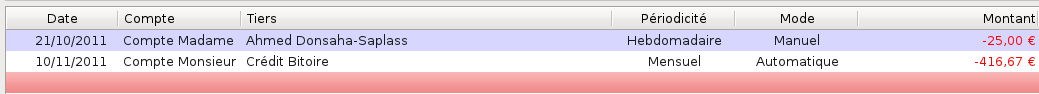
\includegraphics[scale=0.5]{image/screenshot/planned_transactions_list}
\end{center}
\caption{Liste des opérations planifiées}
\label{planned-transactions-list-img}
\end{figure}
% image centrée
\fi

Elle affiche en haut la barre des libellés des colonnes. Vous pouvez \indexword{élargir ou rétrécir une colonne}\index{colonne !largeur} en cliquant sur le séparateur entre deux colonnes et en le déplaçant. Pour rétablir la \indexword{largeur des colonnes}\index{colonne !largeur} à leur valeur par défaut, sélectionnez le menu \menu{Affichage - Réinitialiser la largeur des colonnes}.

Vous pouvez déplacer la liste des opérations planifiées vers le haut ou vers le bas avec la molette de la souris, ou bien avec la souris et l'ascenseur vertical. Le déplacement éventuel vers la gauche ou la droite se fait avec la souris et l'ascenseur horizontal.

% espace pour changement de thème
\vspacepdf{5mm}
Chaque opération est affichée sur une seule ligne et au maximum six colonnes, ce qui fait au maximum six champs d'information pour chaque opération planifiée. Les champs d'affichage, ainsi que les \indexword{libellés des colonnes}\index{colonne !libellé}, sont les suivants :
\begin{itemize}
	 \item \menu{Date} : la date de l'opération ;
	 \item \menu{Compte} : le compte concerné ;
	 \item \menu{Tiers} ;
	 \item \menu{Périodicité} : la périodicité de l'opération ;
	 \item \menu{Mode} : le mode d'exécution, automatique ou manuel ; 
	 \item \menu{Montant} : le montant de l'opération ; un \indexword{montant négatif}\index{montant !négatif} est affiché en rouge{\couleur}.
% saut de ligne pour indentation correcte de la note dans la liste

\textbf{Note} : si l'affichage du champ \menu{Remarques} a été demandé, il s'affiche à la place des champs \menu{Périodicité} et \menu{Mode}, ce qui ne fait plus que cinq colonnes et cinq champs affichés.	 
\end{itemize}

% espace pour changement de thème
\vspacepdf{5mm}
Une ligne supplémentaire vide s'affiche juste en-dessous de la dernière ligne d'opération, et sert à créer une nouvelle opération planifiée (voir la section \vref{plannedtransactions-new}, \menu{Nouvelle opération planifiée}).

% espace pour changement de thème
\vspacepdf{5mm}
Pour des raisons de lisibilité de l'affichage, Grisbi présente une alternance de couleurs de fond violet et blanc{\couleurs} à chaque ligne.

% espace pour changement de thème
\vspacepdf{5mm}
En cliquant sur l'outil  \menu{Affichage} dans la barre d'outils, une liste déroulante vous permet de choisir plusieurs modes d'affichage des prochaines occurrences :
% espace avant image 5mm
\vspacepdf{3mm}

\begin{itemize}
	\ifIllustration
	% image entourée par une liste (picins)
	% pas de référence à l'illustration car erreur de numéro de figure avec picins.
	% supprimé car en html les figures entourées ne sont pas numérotées, et la numérotation des figures centrées décalée par rapport au pdf
	%\piccaption{Choix des modes d'affichage}
	\label{planned-transactions-display-img}
	\parpic[r]{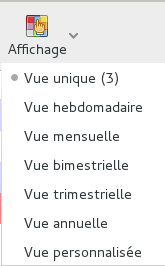
\includegraphics[scale=0.50]{image/screenshot/planned_transactions_display}}
	% image entourée par une liste (picins)
	\fi
	 \item \menu{Vue unique} : la prochaine occurrence de chaque opération ; 
	 \item \menu{Vue hebdomadaire} ; à échéance de 7 jours ;
	 \item \menu{Vue mensuelle} : à échéance de 30 jours ;
	 \item \menu{Vue bimestrielle} : à échéance de 60 jours  ;
	 \item \menu{Vue trimestrielle} : à échéance de 90 jours  ;
	 \item \menu{Vue annuelle} : à échéance d'un an ;
	 \item \menu{Vue personnalisée} : à échéance d'un nombre quelconque de jours, semaines, mois ou années.
% espace pour Note ou Attention à la ligne dans une liste

	 % espace pour changement de thème
	 \vspacepdf{3mm}   
	 L'affichage courant y est indiqué par une coche, ainsi que le nombre d'opérations dans cette vue.
\end{itemize}

\ifIllustration
% espace après image entourée
\vspacepdf{13mm}
\vspacehevea{7mm}
\else
\vspacepdf{5mm}
\fi

Si vous choisissez l'affichage personnalisé, une nouvelle fenêtre affiche deux listes déroulantes pour choisir le nombre et la période \ifIllustration désirés\refimage{planned-transactions-display-custom-img}.

% image centrée 
\begin{figure}[htbp]
\begin{center}
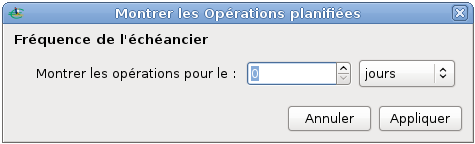
\includegraphics[scale=0.5]{image/screenshot/planned_transactions_display_custom}
\end{center}
\caption{Choix de l'affichage de la période personnalisée}
\label{planned-transactions-display-custom-img}
\end{figure}
% image centrée 
\else désirés.
\fi

\ifIllustration
\else
% saut de page pour titre solidaire
\newpage
\fi


\subsection{Tris\label{plannedtransactions-list-sorts}}

Pour changer l'ordre d'affichage des opérations planifiées, vous pouvez faire un \indexword{tri sur les opérations}\index{tri !opérations} sur un des champs d'information ; procédez comme suit :

\begin{enumerate}
	  \item cliquez sur le libellé de la colonne qui contient le champ d'information choisi comme critère de \gls{tri} ; les seuls critères de tri possibles sont la \menu{Date}, le \menu{Compte} et le \menu{Tiers}.
	  \item toutes les opérations s'affichent, triées selon le critère choisi ;
	  \item un petit triangle noir apparaît à droite du libellé de la colonne ; il pointe vers le bas si le tri est ascendant, vers le haut si le tri est descendant ;

\textbf{Note} : ces triangles peuvent être remplacés, en fonction du thème de l'environnement de bureau ou du gestionnaire de fenêtres que vous utilisez, par d'autres caractères tels que +, -, >, <, etc.
	  \item cliquez sur ce triangle pour changer l'ordre du tri.
\end{enumerate}


\section{Formulaire de saisie des opérations planifiées\label{plannedtransactions-form}}


Le formulaire de saisie des opérations planifiées s'affiche en-dessous de la liste des opérations planifiées. Il est similaire au formulaire de saisie des opérations ordinaires, mais il comprend, dans sa partie supérieure, une ligne supplémentaire de trois à six champs pour \ifIllustration indiquer\refimage{planned-transactions-form-img} :
\else indiquer :
\fi

\ifIllustration
% image centrée
\begin{figure}[htbp]
\begin{center}
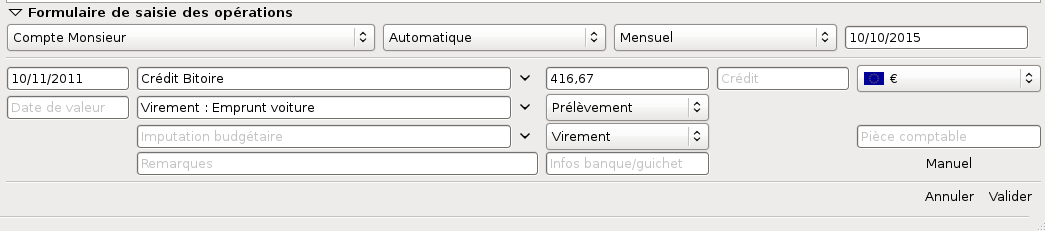
\includegraphics[scale=0.5]{image/screenshot/planned_transactions_form}
\end{center}
\caption{Formulaire de saisie des opérations planifiées}
\label{planned-transactions-form-img}
\end{figure}
% image centrée
\fi

\begin{itemize}
	\item le compte affecté ; dans le cas d'un virement entre deux comptes, vous pouvez sélectionner l'un ou l'autre des deux comptes (origine ou destination) ; le type de l'opération (débit ou crédit) doit être renseigné dans le champ adéquat, et la contre-opération sera automatiquement créée dans l'autre compte au moment de l'exécution de l'opération planifiée ;
	
	\item le mode d'exécution :
	
		\begin{itemize}
			\item \menu{Manuel} : vous devrez exécuter manuellement la saisie dans le formulaire en sélectionnant la fonction \menu{Exécuter} dans la barre de fonctions ou dans le menu contextuel (voir la section \vref{plannedtransactions-execution}, \menu{Exécution d'une opération planifiée},
			\item \menu{Automatique} : l'opération sera automatiquement saisie dans la liste des opérations à la date programmée ;
		\end{itemize}
	
	\item la \menu{Périodicité} :
		\begin{itemize}
			\item \menu{Une fois},
			\item \menu{Hebdomadaire},
			\item \menu{Mensuelle},
			\item \menu{Bimestrielle},
			\item \menu{Trimestrielle},
			\item \menu{Annuelle},
			\item \menu{Personnalisée} ; dans ce cas, vous devrez préciser plus finement le nombre de périodes entre chaque saisie ou demande de validation de l'opération, ainsi que la période voulue (jours, semaines, \ifIllustration mois, années)\refimage{planned-transactions-frequency_custom-img} ;
	\else mois, années) ;
	\fi
	
	\ifIllustration
	% image centrée
	\begin{figure}[htbp]
	\begin{center}
	
\includegraphics[scale=0.5]{image/screenshot/planned_transactions_frequency_custom}
	\end{center}
	\caption{Saisie d'une périodicité personnalisée}
	\label{planned-transactions-frequency_custom-img}
	\end{figure}
	% image centrée
	\fi
	\end{itemize}
\item la \menu{Date limite} des échéances ; le choix par défaut est \menu{Aucune} ; un double-clic ou la combinaison de touches \key{Ctrl}\key{Entrée} dans ce champ ouvre un calendrier (voir la section \vref{plannedtransactions-calendar}, \menu{Calendrier et prévisions}) ; vous pouvez aussi saisir manuellement la date en utilisant les multiples combinaisons de touches telles que décrites dans la section \vref{transactions-new-dates}, \menu{Saisie de date au clavier}.
\end{itemize}

% espace pour changement de thème
\vspacepdf{5mm}
La partie inférieure du formulaire est strictement identique au formulaire de saisie des opérations ordinaires, et est géré de la même manière \ifIllustration \refimage{planned-transactions-form-img},
\else manière,
\fi
 voir la section \vref{transactions-form}, \menu {Formulaire de saisie}.

% espace pour changement de thème
\vspacepdf{5mm}
Une fois le formulaire affiché, un menu contextuel accessible par un clic-droit dans un champ de saisie permet d'effectuer les actions suivantes :

\begin{itemize}
	 \item \menu{Couper} (la sélection) ;
	 \item \menu{Copier} (la sélection) ;
	 \item\menu{Coller} (la sélection) ;
	 \item \menu{Supprimer} (la sélection) ;
	 \item \menu{Tout sélectionner} (dans le champ de saisie) ;
	 \item \menu{Méthodes de saisie} ;
	 \item \menu{Insérer un caractère de contrôle Unicode}.
\end{itemize}

Le choix \menu{\gls{methodes de saisie}} permet de changer les caractères accentués.

Le choix \menu{Insérer un \gls{caractere de controle Unicode}} permet d'insérer un code Unichar qui modifie la présentation ; par exemple RLO (forçage droite-à-gauche) renverse l'ordre des lettres et la position du texte.

% espace pour changement de thème
\vspacepdf{5mm}
De plus, un autre menu contextuel accessible par un clic-droit dans le formulaire de saisie, dans une zone grise en dehors des champs de saisie, permet d'accéder à la configuration du formulaire, en sélectionnant  \menu{Configurer le formulaire} (voir la section \vref{setup-form}, \menu{Formulaire des opérations}).

% espace pour changement de thème
\vspacepdf{5mm}
Notez que le choix des types d'opérations est nécessairement lié au type du compte sélectionné (voir la section \vref{accounts-type}, \menu{Types de compte de Grisbi}).


\section{Calendrier et prévisions\label{plannedtransactions-calendar}}


Un calendrier s'affiche à la place du bas du panneau de navigation. Il indique en caractères gras les dates auxquelles des opérations planifiées de tous les comptes arrivent à échéance, et sur fond bleu{\couleur} la date du jour.

Cliquez sur le calendrier pour le sélectionner. Vous pouvez le parcourir avec la souris ou le clavier :
% espace avant image 5mm
\vspacepdf{3mm}

\begin{itemize}
	% image entourée par une liste ( picins)
	% pas de référence à l'illustration car erreur de numéro de figure avec picins.
	\ifIllustration
	% supprimé car en html les figures entourées ne sont pas numérotées, et la numérotation des figures centrées décalée par rapport au pdf
	%\piccaption{Calendrier des opérations planifiées}
	\label{planned-transactions-calendar-img}
	\parpic[r]{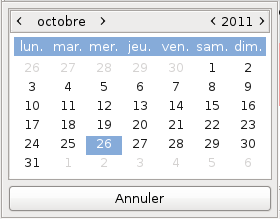
\includegraphics[scale=0.5]{image/screenshot/planned_transactions_calendar}}
	% image entourée par une liste ( picins)
	\fi
	
	\item les touches \key{Flèche Gauche} ou \key{Flèche Droite}, permettent de passer au jour précédent ou suivant ;
	\item les touches \key{Flèche Haut} ou \key{Flèche Bas} permettent de passer à la semaine précédente ou suivante ;
	\item la combinaison de touches \key{Ctrl}\key{Flèche Gauche} ou \newline \key{Ctrl}\key{Flèche Droite} permet de passer au mois précédent ou suivant ;
	\item la combinaison de touches \key{Ctrl}\key{Flèche Haut} ou \newline \key{Ctrl}\key{Flèche Bas} permet de passer à l'année précédente ou suivante.
\end{itemize}

\ifIllustration
% espace après image entourée
\vspacepdf{5mm}
\vspacehevea{10mm}
\fi


\section{Sélection d'une opération planifiée\label{plannedtransactions-selection}}


Pour sélectionner une opération planifiée, vous avez deux moyens :

\begin{itemize}
	 \item cliquer sur sa ligne ;
	 \item déplacer la sélection avec les touches du clavier \key{Flèche Haut} et \key{Flèche Bas}.
\end{itemize}

L'opération apparaît alors sur fond bleu{\couleur} et ses détails s'affichent dans le formulaire.

% espace pour changement de thème
\vspacepdf{5mm}
Un menu contextuel est disponible sur la liste des opérations planifiées. Un clic-droit sur la ligne d'une opération permet les fonctions suivantes, selon le contexte :
% espace avant image 5mm
\vspacepdf{3mm}

\begin{itemize}
	% image entourée par une liste (picins)
	% pas de référence à l'illustration car erreur de numéro de figure avec picins.
	\ifIllustration
	% supprimé car en html les figures entourées ne sont pas numérotées, et la numérotation des figures centrées décalée par rapport au pdf
	%\piccaption{Menu contextuel de la liste des opérations planifiées}
	\label{planned-transactions-context-img}
	\parpic[r]{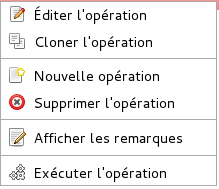
\includegraphics[scale=0.5]{image/screenshot/planned_transactions_context}}
	% image entourée par une liste (picins)
	\fi
	 \item \menu{Éditer l'opération} ;
	 \item \menu{Cloner l'opération} ;
	 \item \menu{Nouvelle opération} ;
	 \item \menu{Supprimer l'opération} ;
	 \item \menu{Afficher les remarques} ou \menu{Afficher Périodicité/Mode} ;	 
	 \item \menu{Exécuter l'opération}.
\end{itemize}

\ifIllustration
% espace après image entourée
\vspacepdf{11mm}
\fi


\section{Nouvelle opération planifiée\label{plannedtransactions-new}}


La saisie d'une opération planifiée se fait d'une manière similaire à la saisie d'une opération ordinaire.

Vous pouvez ouvrir le formulaire de saisie avec l'une de ces méthodes :

\begin{itemize}
	 \item sélectionnez la ligne vide en bas de la liste des opérations et appuyez sur la touche \key{Entrée} ;
	 \item double-cliquez sur la ligne vide ;
	 \item dans la barre d'outils, cliquez-gauche sur l'outil \menu{Nouvelle échéance} ;
	 \item dans le menu contextuel, sélectionnez le choix \menu{Nouvelle opération} ;
	 \item cliquez-gauche sur le petit triangle d'affichage/masquage à gauche du libellé \menu{Formulaire de saisie des opérations}, tout en bas du pavé des détails. 
\end{itemize}

\textbf{Note} : ce triangle peut être remplacé, en fonction du thème de l'environnement de bureau ou du gestionnaire de fenêtres que vous utilisez, par d'autres caractères tels que +, -, >, <, etc.

% espace pour changement de thème
\vspacepdf{5mm}
Renseignez les champs avec les paramètres de votre opération planifiée. Pour plus de détails sur la saisie de ces paramètres dans le formulaire, voir les sections \vref{plannedtransactions-form}, \menu{Formulaire de saisie des opérations planifiées} et \vref{plannedtransactions-calendar}, \menu{Calendrier et prévisions}. 


\section{Ventilation d'une opération planifiée\label{plannedtransactions-breakdown}}


La ventilation d'une opération planifiée se fait d'une manière similaire à la ventilation d'une opération ordinaire. Une fois que vous avez renseigné les champs  de la première ligne du formulaire (voir la section \vref{plannedtransactions-form}, \menu{Formulaire de saisie des opérations planifiées}), saisissez les autres paramètres de l'opération dans la partie inférieure de ce formulaire (voir la section \vref{transactions-form}, \menu{Formulaire de saisie}), et procédez à la saisie de l'opération planifiée ventilée, comme décrit précisément dans la section \vref{transactions-breakdown}, \menu{Ventilation d'une opération}.


\section{Modification d'une opération planifiée\label{plannedtransactions-modify}}


Pour modifier une opération planifiée, procédez comme suit :

\begin{enumerate}
	 \item sélectionnez-la dans la liste ;
	 \item cliquez sur l'outil \menu{Éditer} dans la barre d'outils, ou cliquez-droit sur la ligne de l'opération et sélectionnez \menu{Éditer l'opération} dans le menu contextuel ;
	 \item le formulaire de saisie s'ouvre sur le champ  \menu{Date} : vous pouvez alors modifier toutes les données de l'opération ;
	 \item validez par le bouton \menu{Valider}.
\end{enumerate}


\section{Clonage d'une opération planifiée\label{plannedtransactions-duplicate}}


Pour cloner une opération planifiée, sélectionnez-la pour qu'elle s'affiche dans le formulaire de saisie, puis utilisez l'une de ces deux méthodes :

\begin{itemize}
	 \item dans la barre de menus, sélectionnez \menu{Édition - Cloner l'opération} ;
	 \item dans le menu contextuel, sélectionnez \menu{Cloner l'opération}.
\end{itemize}

% espace pour changement de thème
\vspacepdf{5mm}
L'opération sélectionnée précédemment apparaît toujours sur fond  rouge{\couleur}, et l'opération clonée s'affiche dans une nouvelle ligne en-dessous.

Vous pouvez alors éditer cette nouvelle opération, par exemple en modifiant la date.


\section{Remarques des opérations planifiées\label{plannedtransactions-comments}}


Vous pouvez afficher ou cacher les remarques de deux manières :

\begin{itemize}
	 \item cliquez sur l'outil \menu{Remarques} dans la barre d'outils ;
	 \item cliquez-droit sur la ligne de l'opération et sélectionnez \menu{Afficher/Masquer les remarques} dans le menu contextuel.
\end{itemize}

Les remarques de toutes les opérations s'affichent alors à la place des colonnes \menu{Périodicité} et \menu{Mode} dans la liste des opérations planifiées. Recommencer la même séquence réaffiche les colonnes \menu{Périodicité} et \menu{Mode} à la place de la \ifIllustration colonne \menu{Remarques}\refimage{planned-transactions-list-comments-img}.

% image centrée
\begin{figure}[htbp]
\begin{center}
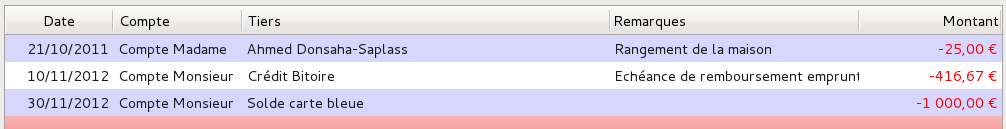
\includegraphics[scale=0.5]{image/screenshot/planned_transactions_list_comments}
\end{center}
\caption{Affichage des remarques des opérations planifiées}
\label{planned-transactions-list-comments-img}
\end{figure}
% image centrée
\else colonne \menu{Remarques}.
\fi

\ifIllustration
% espace après légende 10mm
\vspacepdf{-6mm}
\fi


\section{Exécution d'une opération planifiée\label{plannedtransactions-execution}}


La fonction \menu{Exécuter une opération planifiée} sert uniquement à faire la recopie, dans le formulaire de saisie, de l'occurrence d'une opération sélectionnée dans la liste des opérations planifiées. Pour que cette occurrence soit effectivement transférée dans la liste des opérations du compte concerné, il est nécessaire de valider ensuite le formulaire de saisie, après avoir éventuellement modifié l'opération. 

% espace pour changement de thème
\vspacepdf{5mm}
Pour exécuter une occurrence d'une opération planifiée, procédez comme suit :

\begin{enumerate}
	 \item sélectionnez-la dans la liste ;
	 \item cliquez sur l'outil \menu{Exécuter} dans la barre d'outils, ou cliquez-droit sur la ligne de l'opération et sélectionnez \menu{Exécuter l'opération} dans le menu contextuel ;
	 \item l'occurrence sélectionnée de l'opération s'affiche dans le formulaire de saisie ; vous pouvez alors la modifier selon votre besoin ;
	 \item validez par le bouton \menu{Valider} ; l'occurrence de l'opération est transférée dans la liste des opérations du compte concerné, et la liste des opérations planifiées affiche l'occurrence suivante (si elle existe, car l'opération planifiée peut être unique) de l'opération planifiée. 
\end{enumerate}

% espace avant Attention ou Note  : 5 mm
\vspacepdf{5mm}
\textbf{Note} : après cette validation, la recopie est faite sans autre avertissement.

% espace pour changement de thème
\vspacepdf{5mm}
Vous pouvez aussi vérifier que l'occurrence exécutée de l'opération planifiée se trouve maintenant bien dans  la liste des opérations du compte concerné.


\section{Suppression d'une opération planifiée\label{plannedtransactions-remove}}


Pour supprimer une opération planifiée, procédez comme suit :

\begin{enumerate}
	 \item sélectionnez-la dans la liste ;
	 \item cliquez sur l'outil \menu{Supprimer} dans la barre d'outils, ou cliquez-droit sur la ligne de l'opération et sélectionnez \menu{Supprimer l'opération} dans le menu contextuel ;
	 \item une  boîte de dialogue s'ouvre et vous propose de supprimer, soit toutes les occurrences (toutes les opérations, courante et futures, seront supprimées), soit uniquement l'occurrence courante (seule l'opération \ifIllustration affichée sera supprimée)\refimage{planned-transactions-delete-img} ;
	% image centrée
	\begin{figure}[htbp]
	\begin{center}
	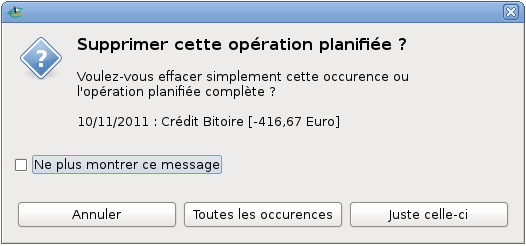
\includegraphics[scale=0.5]{image/screenshot/planned_transactions_delete}
	\end{center}
	\caption{Suppression d'une opération planifiée}
	\label{planned-transactions-delete-img}
	\end{figure}
	% image centrée
	\else affichée sera supprimée) ;
	\fi
	 \item faites votre choix, la suppression est exécutée immédiatement.
\end{enumerate}

 % espace avant Attention ou Note  : 5 mm
\vspacepdf{3mm}
\strong{Attention} : immédiatement après le choix entre \menu{Toutes les occurrences} et \menu{Juste celle-ci}, la suppression est exécutée sans autre avertissement. 

 % espace avant Attention ou Note  : 5 mm
\vspacepdf{4mm}
\strong{Attention} : la suppression d'une opération planifiée est \indexword{irréversible}\index{opération !irréversible} ! 


\myclearemptydoublepage

%%%%%%%%%%%%%%%%%%%%%%%%%%%%%%%%%%%%%%%%%%%%%%%%%%%%%%%%%%%%%%%%%
% Contents : The search chapter 
% $Id : grisbi-manuel-search.tex, v 0.4 2002/10/27 Daniel Cartron
% $Id : grisbi-manuel-search.tex, v 0.5.0 2004/06/01 Loic Breilloux
% $Id : grisbi-manuel-search.tex, v 0.6.0 2011/11/17 Jean-Luc Duflot
% $Id : grisbi-manuel-search.tex, v 0.8.9 2012/04/27 Jean-Luc Duflot
% $Id : grisbi-manuel-search.tex, v 1.0 2014/02/12 Jean-Luc Duflot
%%%%%%%%%%%%%%%%%%%%%%%%%%%%%%%%%%%%%%%%%%%%%%%%%%%%%%%%%%%%%%%%%

\chapter{Recherches\label{search} }

Vous pouvez avoir besoin de consulter une opération plus ou moins récente. Pour cela, Grisbi propose plusieurs méthodes de recherche d'opérations.


\section{Recherche dans les listes d'opérations et d'opérations planifiées\label{search-list} }


La liste des opérations d'un compte et la liste des opérations planifiées permettent de faire des tris, basés sur un seul critère de tri à la fois. La méthode est décrite :

\begin{itemize}
	 \item pour les opérations d'un compte, dans la section \vref{transactions-list-sorts}, \menu{Tris} ;
	 \item pour les opérations planifiées, dans la section \vref{plannedtransactions-list-sorts}, \menu{Tris}.
\end{itemize}

%espace pour changement de thème
\vspacepdf{5mm}
Une fois la liste triée, vous pouvez identifier plus rapidement l'opération qui vous intéresse.


\section{Recherche dans les tiers, catégories ou imputations budgétaires\label{search-simple} }


Si vous recherchez une opération dont vous connaissez le tiers, la catégorie ou l'imputation budgétaire, procédez comme suit :

\begin{itemize}
	 \item ouvrez l'onglet tiers, catégorie ou imputation budgétaire selon le cas ;
	 \item sélectionnez une ligne quelconque ;
	 \item tapez au clavier le ou les premiers caractères du tiers, catégorie ou imputation budgétaire recherché : ils s'affichent alors dans une petite fenêtre en bas et à droite du pavé des détails, et la sélection se place sur la ligne du terme recherché ;
	 \item déroulez le contenu de cette sélection pour afficher ses opérations ;
	 \item double-cliquez sur l'opération recherchée : la liste des opérations du compte concerné s'affiche, dans laquelle l'opération s'affiche sur fond rouge{\couleur}.	 	 	 
\end{itemize}

%espace pour changement de thème
\vspacepdf{5mm}

Pour plus de détails, reportez-vous respectivement aux sections \vref{thirdparties-list}, \menu{Liste des tiers}, \vref{categories-list}, \menu{Liste des catégories et des sous-catégories}, ou \vref{budgetarylines-list}, \menu{Liste des imputations budgétaires} et suivantes.


\section{Recherche par états\label{search-advanced} }


Si la méthode ci-dessus ne convient pas, une recherche plus élaborée passe par la création d'un état spécifique à cette recherche. Pour cela vous pouvez utiliser l'état pré-formaté \menu{Recherche}, qui vous affichera toutes les informations de toutes les opérations pour tous les comptes de  l'année en cours.

%espace pour changement de thème
\vspacepdf{5mm}
Il vous faudra probablement ajuster le choix dans la date, et préciser d'autres critères, tels un montant (qui doit être affecté d'un signe \og moins \fg{} pour une dépense) ou une \indexword{chaîne de caractères}\index{chaîne de caractères} à rechercher. 

 % espace avant Attention ou Note  : 5 mm
\vspacepdf{5mm}
\textbf{Note} : si vous sélectionnez \menu{Toutes les dates}, la génération de l'état risque d'être assez longue. D'une manière générale, moins les critères seront précis, plus cette génération sera longue et plus les résultats seront nombreux.

%espace pour changement de thème
\vspacepdf{5mm}
Une fois l'opération trouvée dans l'état, et si les opérations sont configurées comme \indexword{cliquables}\index{opération !cliquable} (voir le paragraphe \vref{reportscreation-display-transactions-clickable}, \menu{Opérations cliquables}), cliquez sur sa ligne pour afficher directement le détail de l'opération.

%espace pour changement de thème
\vspacepdf{5mm}
Pour savoir comment créer un état, voir le chapitre \vref{reportscreation}, \menu{Création d'un état}.



\myclearemptydoublepage

%%%%%%%%%%%%%%%%%%%%%%%%%%%%%%%%%%%%%%%%%%%%%%%%%%%%%%%%%%%%%%%%%
% Contents : The third parties chapter
% $Id : grisbi-manuel-third.tex, v 0.4 2002/10/27 Daniel Cartron
% $Id : grisbi-manuel-third.tex, v 0.5.0 2004/06/01 Loic Breilloux
% some of its content was in tips chapter : 
% $Id : grisbi-manuel-tips.tex, v 0.4 2002/10/27 Daniel Cartron
% $Id : grisbi-manuel-third.tex, v 0.6.0 2011/11/17 Jean-Luc Duflot
% some of its content was in tips chapter :
% $Id : grisbi-manuel-tips.tex, v 0.5.0 2004/06/01 Loic Breilloux
% $Id : grisbi-manuel-third.tex, v 0.8.9 2012/04/27 Jean-Luc Duflot
% $Id : grisbi-manuel-third.tex, v 1.0 2014/02/12 Jean-Luc Duflot
%%%%%%%%%%%%%%%%%%%%%%%%%%%%%%%%%%%%%%%%%%%%%%%%%%%%%%%%%%%%%%%%%

\chapter{Tiers\label{thirdparties}}


On appelle tiers la personne ou plus généralement l'organisation avec qui on a
une relation financière, par exemple un ami, un commerçant ou une administration.  Ne pas confondre avec la catégorie, qui définit  la nature de cette relation, par exemple \og Loisirs \fg{} ou \og Habillement \fg{}. D'une autre manière, \emph{qui} et \emph{quoi}\ldots

Bien sûr, si vous changez de fournisseur sans cesse, vous pouvez créer un tiers fournisseur générique (ex : \emph{Station-service}) mais votre comptabilité sera moins précise.

Outre ces tiers, peuvent aussi exister ceux que l'on pourrait appeler des 
\indexword{\emph{tiers financiers}}\index{tiers !financiers}. En effet, lorsque vous faites un virement de compte à compte, il est intéressant de créer un tiers spécifique pour ce genre d'opération, par exemple 
\emph{Alimentation des comptes d'épargne}, ou bien \emph{Remise de chèques}, ou encore \emph{Régularisation d'avances}. Ceci vous permettra ultérieurement une analyse plus fine de vos finances. 

% espace pour changement de thème
\vspacepdf{5mm}
L'onglet \menu{Tiers} sert à gérer tous les tiers de votre fichier de comptes.

%espace pour changement de thème
\vspacepdf{5mm}
Pour avoir accès à la gestion des tiers, cliquez sur \menu{Tiers} dans le panneau de navigation, ou sélectionnez \menu{Tiers} avec la barre d'information (voir le chapitre \vref{home}, \menu{Accueil}).

%espace pour changement de thème
\vspacepdf{5mm}
La barre d'information affiche, à gauche, le nom du tiers sélectionné dans le pavé des détails et, complètement à droite, le solde des opérations affectées.

%espace pour changement de thème
\vspacepdf{5mm}
Le pavé des détails affiche deux éléments :
\begin{itemize}
	 \item la barre d'outils ;
	 \item la liste des tiers.
\end{itemize}


\section{Barre d'outils\label{thirdparties-functions}}


La barre d'outils des tiers présente les fonctions suivantes  :

\begin{itemize}
	 \item \menu{Nouveau tiers} : ouvre une fenêtre pour créer un nouveau tiers ;
	 \item \menu{Supprimer} : supprime le tiers sélectionné ;
	 \item \menu{Éditer} : ouvre une fenêtre pour modifier le nom ou la description du tiers sélectionné ;
	 \item \menu{Affichage} : ouvre un menu déroulant pour afficher soit la \menu{Vue des tiers uniquement}, soit la \menu{Vue complète}, pour tous les tiers avec leurs opérations, ainsi que le choix d'\menu{Afficher les tiers inutilisés} ;
	 \item \menu{Gérer les tiers} : ouvre l'assistant de gestion des tiers ;
	 \item \menu{Supprimer les tiers inutilisés} : permet de supprimer les tiers n'ayant aucune opération.
\end{itemize}

%espace pour changement de thème
\vspacepdf{5mm}
% FONCTION SUPPRIMÉE La barre d'outils peut être déplacée dans l'écran en cliquant sur sa poignée (petit rectangle vertical à gauche de la barre) et en la déplaçant. Pour la réattacher à son emplacement d'origine dans le pavé des détails, la remettre en haut de la fenêtre, le haut de la poignée placé sur le petit trait qui visualise sa place d'origine.


\section{Liste des tiers\label{thirdparties-list}}


La liste des tiers s'affiche dans le panneau des \ifIllustration détails\refimage{thirdparties-list-img}.
\else détails.
\fi
% image centrée
\ifIllustration
\begin{figure}[htbp]
\begin{center}
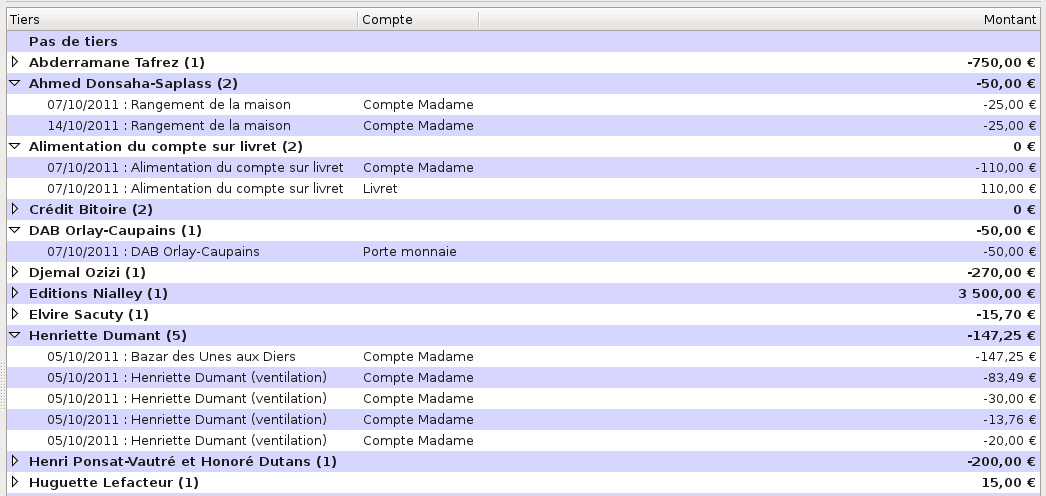
\includegraphics[scale=0.5]{image/screenshot/thirdparties_list}
\end{center}
\caption{Liste des tiers}
\label{thirdparties-list-img}
\end{figure}
% image centrée
\fi

Elle affiche en haut la barre des libellés des colonnes ; ses champs d'affichage sont les suivants :
\begin{itemize}
	 \item le nom du tiers ;
	 \item le compte concerné ;
	 \item le montant total des opérations affectées à ce tiers, et le montant de chaque opération si la ligne du tiers est déroulée.
\end{itemize}

%espace pour changement de thème
\vspacepdf{5mm}
Vous pouvez déplacer la liste des tiers vers le haut ou vers le bas avec la molette de la souris, ou bien avec la souris et l'ascenseur vertical. Le déplacement éventuel vers la gauche ou la droite se fait avec la souris et l'ascenseur horizontal.

%espace pour changement de thème
\vspacepdf{5mm}
La liste des tiers affiche tous les tiers de votre fichier de comptes par ordre alphabétique, avec une seule exception : le premier tiers affiché est toujours le tiers de libellé \indexword{\menu{Pas de tiers}}\index{tiers !pas de tiers}, qui reçoit toutes les opérations dont le tiers n'est pas défini.


Le nombre d'opérations affectées à chaque tiers s'affiche, entre parenthèses, à la suite de son nom, et le montant total des opérations affectées à ces tiers s'affiche dans la colonne \menu{Montant}, à droite sur la même ligne.

% Bogue connu  : en cliquant sur une ligne de tiers, la barre d'information devrait afficher le total, mais n'affiche que 0. 

% espace avant Attention ou Note  : 5 mm
\vspacepdf{5mm}
\textbf{Note} : vous pouvez configurer la \indexword{devise des totaux}\index{devise !totaux} de tous les tiers dans le menu \menu{Édition - Préférences} (voir le paragraphe \vref{setup-display-third-currencies}, \menu{Devises des totaux}).

\ifIllustration
% saut de page pour titre solidaire
\newpage
\fi


\section{Sélection d'un tiers\label{thirdparties-selection}}


Pour sélectionner un tiers, vous avez deux moyens :

\begin{itemize}
	 \item cliquez sur sa ligne ;
	 \item déplacez la sélection avec les touches du clavier \key{Flèche Haut}, \key{Flèche Bas}, \key{Page Haut} ou \key{Page Bas}.
\end{itemize}

Le nom du tiers apparaît alors sur fond rose{\couleur}.


\section{Les opérations d'un tiers\label{thirdparties-transactions}}


Pour \indexword{afficher} les opérations affectées à un tiers\index{affichage !tiers}, cliquez sur le petit triangle à gauche de son nom, ou bien double-cliquez sur sa ligne,
% ou bien sélectionnez-le et appuyez sur la barre d'espace (non fonctionnel) 
ce qui déroule la liste. Les opérations sont alors décrites sur une seule ligne, avec leur date, leur remarque éventuelle, le nom du compte concerné et leur montant.
%le seul moyen de dérouler la liste est de cliquer sur le petit triangle. il devrait y avoir un moyen avec le clavier, comme ça existe avec le formulaire de saisie, où l'on peut utiliser la barre d'espace pour le moyen de paiement, ou la touche flèche bas pour la catégorie..

\textbf{Note} : ces triangles peuvent être remplacés, en fonction du thème de l'environnement de bureau ou du gestionnaire de fenêtres que vous utilisez, par d'autres caractères tels que +, -, >, <, etc.

% espace après Attention ou Note  : 5 mm
\vspacepdf{5mm}

Vous pouvez afficher plusieurs \indexword{tiers déroulés}\index{tiers !déroulés}. Pour ne plus les afficher, \indexword{enroulez les tiers}\index{tiers !enroulés} en cliquant sur le petit triangle à gauche de leur nom, ou bien double-cliquez sur leur ligne. Vous pouvez aussi dérouler ou enrouler tous les tiers de la liste, en cliquant sur l'outil \menu{Affichage}\index{affichage !tiers} dans la barre d'outils et en choisissant \menu{Vue complète}. Pour afficher seulement les tiers, cliquez sur l'outil \menu{Affichage} dans la barre d'outils et choisissez \menu{Vue des tiers uniquement}.

%espace pour changement de thème
\vspacepdf{5mm}
Vous pouvez \indexword{déplacer une opération d'un tiers}\index{tiers !déplacement d'opération} vers un autre tiers de la liste (sauf vers \indexword{\menu{Pas de tiers}}\index{tiers !pas de tiers}), en sélectionnant cette opération et en faisant un glisser-déplacer sur le tiers cible, exactement à l'endroit où son nom est entouré d'une bordure pointillée.

%espace pour changement de thème
\vspacepdf{5mm}
Un \indexword{double-clic sur une ligne d'opération} d'un tiers\index{tiers !double-clic} ferme l'onglet \menu{Tiers}, ouvre l'onglet \menu{Comptes} et le sous-onglet du compte contenant cette opération, sélectionne l'opération concernée et l'affiche dans le formulaire de saisie. De cette façon, cette opération peut être modifiée facilement.


\section{Création d'un tiers\label{thirdparties-new}}


\ifIllustration
% image entourée par un paragraphe ( picins)
% Pas de référence à l'illustration car erreur de numéro de figure avec picins.
% supprimé car en html les figures entourées ne sont pas numérotées, et la numérotation des figures centrées décalée par rapport au pdf
%\piccaption{Création d'un tiers}
\label{thirdparties-new-img}
\parpic[r]{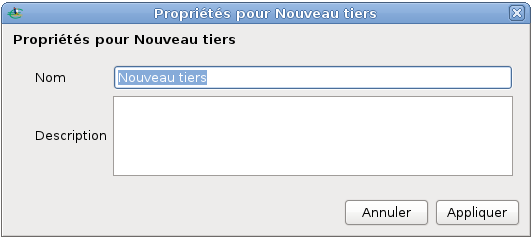
\includegraphics[scale=0.5]{image/screenshot/thirdparties_new}}
% image entourée par un paragraphe ( picins)
\fi

\noindent La façon la plus immédiate pour créer un tiers est de saisir son nom au cours de la saisie d'une nouvelle opération dans l'onglet des comptes (voir la section \vref{transactions-fillcombo}, \menu{Nouveau tiers, catégorie ou imputation budgétaire}) ; mais vous pouvez aussi créer un tiers ici, en cliquant sur l'outil \menu{Nouveau tiers}. Une boîte de dialogue s'ouvre ; renseignez le nom du tiers, et éventuellement une description, puis validez : il apparaît dans la liste des tiers, mais c'est encore un tiers inutilisé, puisqu'aucune opération ne lui est encore affectée (voir la section \vref{thirdparties-unused}, \menu{Tiers inutilisés}).

% espace avant Attention ou Note  : 5 mm
\vspacepdf{5mm}
\textbf{Note} : il n'est pas prévu d'affichage de plus d'informations pour les tiers, par exemple plusieurs champs pour l'adresse, le téléphone, etc. En effet, il nous semble plus intéressant de prévoir dans le futur une liaison avec un gestionnaire de carnet d'adresses de \gls{Gnome} ou de \gls{KDE}, ce qui permettra une gestion beaucoup plus poussée des tiers.

% espace avant Attention ou Note  : 5 mm
\vspacepdf{5mm}
\textbf{Note} : dans tous les cas, un tiers, même inutilisé, s'affiche dans la liste déroulante du formulaire de saisie d'opération, ce qui permet de le sélectionner.


\section{Modification d'un tiers\label{thirdparties-modify}}


Pour modifier un tiers, procédez comme suit :
% espace avant image 5mm
\vspacepdf{3mm}

\begin{enumerate}
	\ifIllustration
	% image entourée par une liste (picins)
	% Pas de référence à l'illustration car erreur de numéro de figure avec picins.
	% supprimé car en html les figures entourées ne sont pas numérotées, et la numérotation des figures centrées décalée par rapport au pdf
	%\piccaption{Propriétés d'un tiers}
	\label{thirdparties-infos-img}
	\parpic[r]{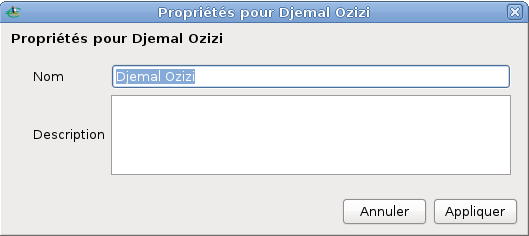
\includegraphics[scale=0.51]{image/screenshot/thirdparties_infos}}
	% image entourée par une liste (picins)	
	\fi
	 \item sélectionnez-le dans la liste ;
	 \item cliquez sur l'outil \menu{Éditer} dans la barre d'outils ;
	 \item une boîte de dialogue s'ouvre : vous pouvez y modifier son nom et sa  description ;
	 \item validez.
\end{enumerate}

\ifIllustration
% espace après légende 10mm
\vspacepdf{5mm}
\fi

\ifIllustration
% espace après image entourée
\vspacehevea{16mm}
\fi


\section{Gestion des tiers\label{thirdparties-management}}


La gestion des tiers permet de modifier le nom de plusieurs tiers à la fois. La méthode consiste à remplacer une chaîne de caractères par une autre en utilisant le \indexword{caractère générique}\index{caractère générique  !\%}  \og  \%  \fg{}, qui remplace tout autre caractère.

Pour gérer les tiers, cliquez sur l'outil \menu{Gérer les tiers} dans la barre d'outils. L'assistant de gestion des tiers s'ouvre, qui comprend quatre étapes ; suivez les instructions données à chaque étape :
\begin{enumerate}
	 \item un avertissement de précautions à prendre avant de continuer ;
	 \item le choix de la \indexword{chaîne de caractères}\index{chaîne de caractères} à remplacer (\menu{Choisir un tiers}) et de celle de remplacement (\menu{Entrez le nouveau tiers}) ; de plus deux options vous sont proposées :
		\begin{itemize}
			 \item \menu{Extraire un numéro à enregistrer dans \No chèque/virement} : si l'ancien tiers contient un numéro qui peut être assimilé à celui d'un chèque ou d'un virement, Grisbi le déplacera dans le champ \og \No chèque/virement \fg{}, mais le numéro de chèque/virement éventuellement déjà présent sera supprimé,
			\item \menu{Sauvegarder les tiers dans les remarques} : tous les tiers seront écrits dans le champ \menu{Remarques}, et les remarques éventuellement déjà présentes seront supprimées ;
			
			\strong{Attention} : si vous cochez ces options, les données existantes (\No chèque ou Remarques) seront remplacées par les nouvelles données (\No intégré dans le nom du tiers ou nom du tiers).
			% espace après Attention ou Note  : 5 mm
			%\vspacepdf{5mm}
		\end{itemize}
	 \item le bilan des remplacements qui vont être effectués ; vous pouvez y 	sélectionner ou désélectionner les remplacements que Grisbi a trouvé à faire selon les critères définis à l'étape précédente ;
	 \item la validation finale.
\end{enumerate}

\ifIllustration
% saut de page pour paragraphe solidaire
\newpage
\fi


\section{Suppression d'un tiers\label{thirdparties-delete}}


Pour supprimer un tiers, procédez comme suit :

\begin{enumerate}
	\ifIllustration
	% image entourée par une liste (picins)
	% Pas de référence à l'illustration car erreur de numéro de figure avec picins.
	\pichskip{7mm}
	% supprimé car en html les figures entourées ne sont pas numérotées, et la numérotation des figures centrées décalée par rapport au pdf
	%\piccaption{Suppression d'un tiers}
	\label{thirdparties-delete-img}
	\parpic[r]{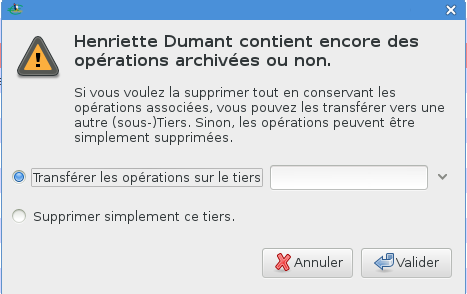
\includegraphics[scale=0.51]{image/screenshot/thirdparties_delete}}
	% image entourée par une liste (picins)	
	\fi
	 \item sélectionnez-le dans la liste ;
	 \item cliquez sur l'outil \menu{Supprimer} dans la barre d'outils ;
	 \item une  boîte de dialogue s'ouvre et vous propose soit de transférer les opérations de ce tiers vers un autre tiers que vous choisissez dans la liste déroulante, soit de le supprimer purement et simplement, \emph{y compris toutes ses opérations} ;
	 \item faites votre choix puis validez.
\end{enumerate}

\ifIllustration
% espace après légende 10mm
\vspacepdf{5mm}
\fi
 
\strong{Attention} : la suppression d'un tiers est \indexword{irréversible}\index{opération !irréversible} !

% espace avant Attention ou Note  : 5 mm
\vspacepdf{5mm}
\textbf{Note} : si le tiers que vous voulez supprimer ne contient aucune opération, aucune boîte de dialogue ne s'ouvrira et Grisbi le supprimera immédiatement.

\ifIllustration
% espace après image entourée
\vspacehevea{2mm}
\fi


\section{Tiers inutilisés\label{thirdparties-unused}}

Un tiers inutilisé est un tiers auquel n'est affectée aucune opération. C'est le cas d'un nouveau tiers quand vous venez juste de le créer avec l'outil \menu{Nouveau tiers}, soit d'un ancien tiers dont toutes les opérations ont été supprimées ou réaffectées vers d'autres tiers.

% espace avant Attention ou Note  : 5 mm
\vspacepdf{5mm}
\textbf{Note} : si vous fermez et réouvrez Grisbi après la création d'un nouveau tiers, il ne sera plus affiché dans la liste des tiers, car il ne contient pas encore d'opération : cela évite l'affichage des tiers inutilisés, qui allonge la liste des tiers souvent très longue ; mais ce tiers apparaîtra dans la liste dès qu'une opération lui aura été affectée.

%espace pour changement de thème
\vspacepdf{5mm}
Pour \indexword{afficher les tiers inutilisés}\index{tiers inutilisés !affichage}\index{affichage !tiers inutilisés}, sélectionnez \menu{Afficher les tiers inutilisés} dans l'outil \menu{Affichage}, qui affiche aussi le nombre de ces tiers.

% espace avant Attention ou Note  : 5 mm
\vspacepdf{5mm}
\textbf{Note} : dans tous les cas, un tiers, même inutilisé, s'affiche dans la liste déroulante du formulaire de saisie d'opération, ce qui permet de le sélectionner.

%espace pour changement de thème
\vspacepdf{5mm}
Pour \indexword{supprimer tous les tiers inutilisés}\index{tiers inutilisés !supprimer}, cliquez sur l'outil \menu{Supprimer les tiers inutilisés} dans la barre d'outils. Une  boîte de dialogue s'ouvre et vous demande la confirmation de cette action. Si vous la validez, une autre boîte affiche le nombre de tiers supprimés.

% espace avant Attention ou Note  : 5 mm
\vspacepdf{5mm}
\strong{Attention} : la suppression des tiers inutilisés est \indexword{irréversible}\index{opération !irréversible} !

\ifIllustration
% saut de page pour titre solidaire
\newpage
\fi


\section{Tiers virtuels\label{thirdparties-virtualCreate}}


Grisbi vous permet d'utiliser des \indexword{tiers virtuels}\index{tiers virtuel} : un tiers virtuel est un \emph{état} qui représente une liste de plusieurs tiers.

Lorsque vous saisissez une opération avec pour tiers un tiers virtuel, Grisbi enregistre, au moment de sa validation, une opération identique (montant, catégorie, imputation budgétaire, moyen de paiement etc.) pour \emph{chacun} des tiers représentés par ce tiers virtuel. Par exemple, vous pouvez saisir en une seule fois un appel à cotisation pour 200 adhérents d'une association, ce qui représente un gain de temps très appréciable \ldots

%espace pour changement de thème
\vspacepdf{5mm}
Pour créer un tiers virtuel, créez un état contenant une liste de tiers : voir le paragraphe \vref{reportscreation-display-general-virtualThird}, \menu{Tiers virtuel}.

% espace avant Attention ou Note  : 5 mm
\vspacepdf{5mm}
\textbf{Note} : comme un tiers virtuel est un état, il ne s'affiche pas dans la liste des tiers, mais dans celle des états, et il est géré de la même manière que les autres états. 

%espace pour changement de thème
\vspacepdf{5mm}
Pour modifier un tiers virtuel, modifiez l'état qui l'a créé : voir la section \vref{reports-modify}, \menu{Modification d'un état}.

%espace pour changement de thème
\vspacepdf{5mm}
Pour supprimer un tiers virtuel, vous avez deux possibilités :

\begin{itemize}
	\item décochez la case \menu{Considérer les tiers de ce rapport comme un tiers virtuel} dans l'état qui le définit, puis validez (voir la section \vref{reports-modify}, \menu{Modification d'un état}) ;
	\item supprimez l'état qui le définit (voir la section \vref{reports-delete}, \menu{Suppression d'un état}).
\end{itemize}

%espace pour changement de thème
\vspacepdf{5mm}
La saisie d'une opération avec un tiers virtuel est décrite dans la section \vref{transactions-virtualThird}, \menu{Saisie d'une opération avec tiers virtuel}.



\myclearemptydoublepage

%%%%%%%%%%%%%%%%%%%%%%%%%%%%%%%%%%%%%%%%%%%%%%%%%%%%%%%%%%%%%%%%%
% Contents : The categories chapter
% $Id : grisbi-manuel-categories.tex, v 0.4 2002/10/27 Daniel Cartron
% $Id : grisbi-manuel-categories.tex, v 0.5.0 2004/06/01 Loic Breilloux
% some of its content was in tips chapter : 
% $Id : grisbi-manuel-tips.tex, v 0.4 2002/10/27 Daniel Cartron
% $Id : grisbi-manuel-categories.tex, v 0.6.0 2011/11/17 Jean-Luc Duflot
% some of its content was in tips chapter :
% $Id : grisbi-manuel-tips.tex, v 0.5.0 2004/06/01 Loic Breilloux
% $Id : grisbi-manuel-categories.tex, v 0.8.9 2012/04/27 Jean-Luc Duflot
% $Id : grisbi-manuel-categories.tex, v 1.0 2014/02/12 Jean-Luc Duflot
%%%%%%%%%%%%%%%%%%%%%%%%%%%%%%%%%%%%%%%%%%%%%%%%%%%%%%%%%%%%%%%%%

\chapter{Catégories\label{categories}}


Pour pouvoir retrouver facilement les opérations, on les classe par catégories, par exemple \og Maison \fg{}, \og Remboursement \fg{}, qui peuvent éventuellement contenir des sous-catégories. En termes de comptabilité, il s'agit d'imputation comptable. Ne pas confondre avec le tiers, qui est celui avec qui on a la relation financière (un fournisseur ou un client).

Grisbi vous permet de faire la distinction entre les imputations comptables et les imputations budgétaires. Mais uniquement si vous le souhaitez.

Une imputation comptable, nommée \menu{Catégorie} dans Grisbi, définit la nature de  l'opération : frais de transport, loisirs, etc. Tandis qu'une imputation budgétaire définit la fonction de l'opération : il s'agit du travail, de la vie courante, des vacances, d'un projet d'aménagement, etc. D'une autre manière, \emph{quoi} et \emph{pourquoi}\ldots{ } Voir aussi le chapitre \vref{budgetarylines}, \menu{Imputations budgétaires}.

 espace pour changement de thème
\vspacepdf{5mm}
Après son installation, Grisbi propose par défaut une liste de catégories. Vous pouvez l'utiliser telle quelle, la modifier selon vos besoins en ajoutant ou en supprimant des catégories ou des sous-catégories, ou bien importer ou exporter une autre liste générée auparavant par Grisbi. Les noms de fichier de ces listes ont pour \indexword{extension} \file{.cgsb} \index{extension !.cgsb}\index{cgsb}, par exemple \file{mes-categories.cgsb}.

% espace avant Attention ou Note  : 5 mm
\vspacepdf{5mm}
\textbf{Note} : toutes vos opérations doivent être affectées à une catégorie \emph{et} à une sous-catégorie, pour deux raisons : elles pourront ainsi être bien classées, donc facilement gérées, et de plus, si elles ne sont pas affectées, elles ne pourront pas être prises en compte dans les budgets prévisionnels.

% espace avant Attention ou Note  : 5 mm
\vspacepdf{5mm}
\textbf{Note} : Il est donc conseillé de bien étudier votre liste de catégories, pour éviter d'avoir à la modifier fréquemment pour cause d'incohérences ou de redondances. Si vous avez vraiment des opérations inclassables, créez une catégorie ou des sous-catégories \og Divers \fg{}, mais n'abusez pas de leur emploi.

% espace pour changement de thème
\vspacepdf{5mm}
L'onglet \menu{Catégories} sert à gérer  toutes les catégories et sous-catégories de votre fichier de comptes.

Pour avoir accès à la gestion des catégories, sélectionnez \menu{Catégories} dans le panneau de navigation ou avec la barre d'information (voir le chapitre \vref{home}, \menu{Accueil}).

La barre d'information affiche, à gauche, le nom de la catégorie et de la sous-catégorie sélectionnées dans le pavé des détails et, complètement à droite, le solde des opérations affectées à la catégorie ou la sous-catégorie sélectionnée.

Le pavé des détails affiche deux éléments :
\begin{itemize}
	 \item la barre d'outils ;
	 \item la liste des catégories.
\end{itemize}


\section{Barre d'outils\label{categories-functions}}


La barre d'outils des catégories présente les fonctions suivantes  :

\begin{itemize}
	 \item \menu{Nouvelle catégorie} : ouvre une fenêtre pour créer une nouvelle catégorie ;
	 \item \menu{Nouvelle sous-catégorie} : ouvre une fenêtre pour créer une 	nouvelle sous-catégorie ;
	 \item \menu{Importer} : permet d'importer une liste de catégories contenue dans un fichier ;
	 \item \menu{Exporter} : permet d'exporter une liste de catégories dans un fichier ;
	 \item \menu{Supprimer} : supprime la catégorie ou la sous-catégorie sélectionnée ;
	 \item \menu{Éditer} : ouvre une fenêtre pour modifier le nom de la catégorie ou de la sous-catégorie sélectionnée ;
	 \item \menu{Affichage} : ouvre un menu déroulant pour afficher la liste des catégories, avec ou sans leurs sous-catégories.
\end{itemize}

% FONCTION SUPPRIMÉE La barre d'outils peut être déplacée dans l'écran en cliquant sur sa poignée (petit rectangle vertical à gauche de la barre) et en la déplaçant. Pour la réattacher à son emplacement d'origine dans le pavé des détails, la remettre en haut de la fenêtre, le haut de la poignée placé sur le petit trait qui visualise sa place d'origine.


\section{Liste des catégories et des sous-catégories\label{categories-list}}


La liste des catégories et sous-catégories s'affiche dans le panneau des \ifIllustration détails\refimage{categories-list-img}.
\else détails.
\fi

\ifIllustration
% image centrée
\begin{figure}[htbp]
\begin{center}
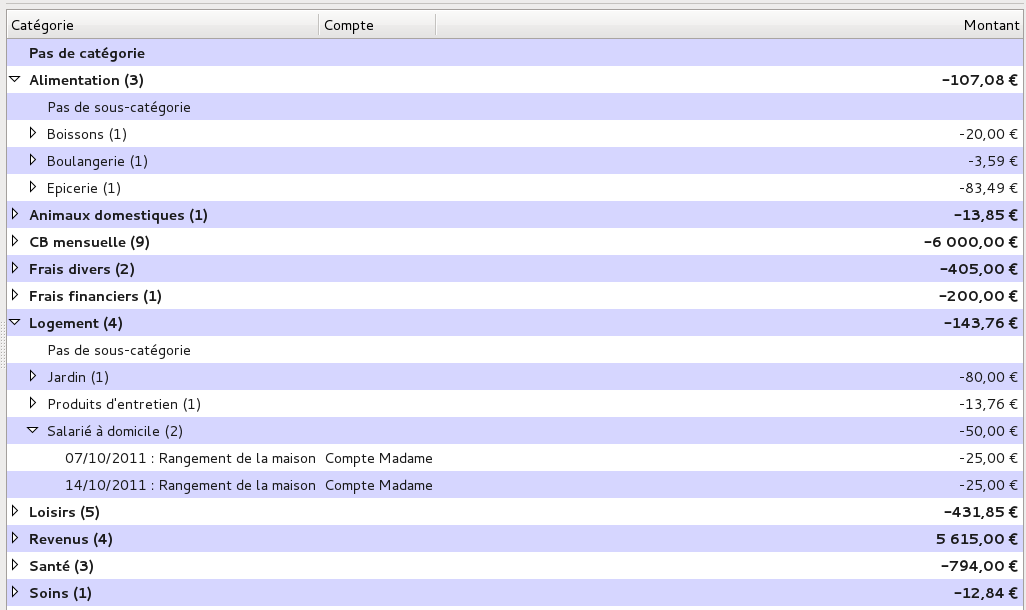
\includegraphics[scale=0.5]{image/screenshot/categories_list.png}
\end{center}
\caption{Liste des catégories et des sous-catégories}
\label{categories-list-img}
\end{figure}
% image centrée
\fi

Elle affiche en haut la barre des libellés des colonnes ; ses champs d'affichage sont les suivants :
\begin{itemize}
	 \item le nom de la catégorie ou de la sous-catégorie ;
	 \item le compte concerné ;
	 \item le montant total des opérations affectées aux  catégories et sous-catégories, et le montant de chaque opération affectée à ces catégories ou sous-catégories si leurs lignes sont déroulées.
\end{itemize}

Vous pouvez déplacer la liste des catégories vers le haut ou vers le bas avec la molette de la souris, ou bien avec la souris et l'ascenseur vertical. Le déplacement éventuel vers la gauche ou la droite se fait avec la souris et l'ascenseur horizontal.

Pour  \indexword{afficher les sous-catégories}\index{affichage !sous-catégories} d'une catégorie, cliquez sur le petit triangle à gauche de son nom, ou bien double-cliquez sur sa ligne ;
% ou bien sélectionnez-la et appuyez sur la barre d'espace (non fonctionnel) 
 cela affiche le libellé  de toutes les sous-catégories, et éventuellement, en première position, \indexword{\menu{Pas de sous-catégorie}}\index{sous-catégories !pas de sous-catégorie}.

\textbf{Note} : ces triangles peuvent être remplacés, en fonction du thème de l'environnement de bureau ou du gestionnaire de fenêtres que vous utilisez, par d'autres caractères tels que +, -, >, <, etc. 

%le seul moyen de dérouler la liste est de cliquer sur le petit triangle. il devrait y avoir un moyen avec le clavier, comme ça existe avec le formulaire de saisie, où l'on peut utiliser la barre d'espace pour le moyen de paiement, ou la touche flèche bas pour la catégorie...

% espace pour changement de thème
\vspacepdf{5mm}
Vous pouvez afficher plusieurs \indexword{catégories déroulées}\index{catégories !déroulées}. Pour ne plus les afficher, \indexword{enroulez les catégories}\index{catégories !enroulées} en cliquant sur le petit triangle à gauche de leur nom, ou bien double-cliquez sur leur ligne. Vous pouvez aussi dérouler ou enrouler toutes les catégories de la liste, en cliquant sur l'outil \menu{Affichage} dans la barre d'outils et en choisissant \menu{Vue des catégories et des sous-catégories}. Pour \indexword{afficher seulement les catégories}\index{affichage !catégories}, cliquez sur l'outil \menu{Affichage} dans la barre d'outils et choisissez \menu{Vue des catégories uniquement}.

Les catégories et sous-catégories de votre fichier de comptes sont affichées par ordre alphabétique, avec deux exceptions : la première catégorie affichée est toujours la catégorie de libellé \indexword{\menu{Pas de catégorie}}\index{catégories !pas de catégorie}, qui reçoit toutes les opérations dont la catégorie n'est pas définie, et, à l'intérieur d'une catégorie, la première sous-catégorie affichée est toujours la sous-catégorie de libellé \indexword{\menu{Pas de sous-catégorie}}\index{sous-catégories !pas de sous-catégorie}, qui reçoit toutes les opérations dont la sous-catégorie n'est pas définie.

Le nombre d'opérations affectées à chaque catégorie ou sous-catégorie s'affiche, entre parenthèses, à la suite de son nom, et le montant total des opérations affectées à ces catégories ou sous-catégories s'affiche dans la colonne \menu{Montant}, à droite sur la même ligne. 

% Bogue connu  : en cliquant sur une ligne de catégories, la barre d'information devrait afficher le total, mais n'affiche que 0. 

% espace avant Attention ou Note  : 5 mm
\vspacepdf{5mm}
\textbf{Note} : vous pouvez configurer la \indexword{devise des totaux}\index{devise !totaux} de toutes les (sous-) catégories dans le menu \menu{Édition - Préférences} (voir la section \vref{setup-display-third-currencies}, \menu{Devises des totaux}).


\section{Sélection d'une catégorie ou d'une sous-catégorie\label{categories-selection}}


Pour sélectionner une catégorie ou une sous-catégorie, vous avez deux moyens :

\begin{itemize}
	 \item cliquez sur sa ligne ;
	 \item déplacez la sélection avec les touches du clavier \key{Flèche Haut}, \key{Flèche Bas}, \key{Page Haut} ou \key{Page Bas}.
\end{itemize}

Le nom de la catégorie ou sous-catégorie apparaît alors sur fond rose{\couleur}.

% espace pour changement de thème
\vspacepdf{5mm}
Un menu contextuel est disponible par un clic-droit sur la liste des catégories ; selon la ligne sélectionnée, vous pouvez exécuter les fonctions suivantes :

\begin{itemize}
	 \item pour une catégorie : \menu{Éditer la catégorie sélectionnée} ;
	 \item pour la sous-catégorie \menu{Pas de sous-catégorie} :
		\begin{itemize}
			 \item si elle est vide : \menu{Éditer la catégorie sélectionnée},
			 \item si elle contient des opérations : \menu{Transférer les opérations dans une autre sous-catégorie},
		\end{itemize}
	 \item pour	une sous-catégorie quelconque :	
		\begin{itemize}
			 \item \menu{Éditer la sous-catégorie sélectionnée},
			 \item \menu{Gérer les sous-catégories},			 
		\end{itemize}		
	 \item pour une opération quelconque : \menu{Transférer des opérations identiques dans une autre sous-catégorie}.	
\end{itemize}

\ifIllustration
% saut de page pour titre solidaire
\newpage
\fi


\section{Les opérations d'une catégorie ou d'une sous-catégorie\label{categories-transactions}}


Une ligne de libellé \menu{Pas de sous-catégorie} se comporte exactement comme une ligne de libellé de sous-catégorie.

Pour afficher les opérations, cliquez sur le petit triangle à gauche du libellé  \menu{Pas de sous-catégorie} ou celui d'une sous-catégorie, ou bien double-cliquez sur sa ligne,
% ou bien sélectionnez-la et appuyez sur la barre d'espace (non fonctionnel),
 ce qui déroule la liste. Les opérations sont alors décrites sur une seule ligne, avec leur date, leur remarque éventuelle, le nom du compte concerné et leur montant.

\textbf{Note} : ces triangles peuvent être remplacés, en fonction du thème de l'environnement de bureau ou du gestionnaire de fenêtres que vous utilisez, par d'autres caractères tels que +, -, >, <, etc. 

%le seul moyen de dérouler la liste est de cliquer sur le petit triangle. il devrait y avoir un moyen avec le clavier, comme ça existe avec le formulaire de saisie, où l'on peut utiliser la barre d'espace pour le moyen de paiement, ou la touche flèche bas pour la catégorie...
 
% espace pour changement de thème
\vspacepdf{5mm}
Vous pouvez afficher plusieurs lignes de \indexword{sous-catégories déroulées}\index{sous-catégories !déroulées}. Pour ne plus les afficher, \indexword{enroulez les opérations}\index{sous-catégories !enroulées} d'une sous-catégorie en cliquant sur le petit triangle à gauche de leur nom, ou bien double-cliquez sur leur ligne. Vous pouvez aussi dérouler ou enrouler toutes les opérations de toutes les catégories et sous-catégories de la liste, en cliquant sur l'outil \menu{Affichage} dans la barre d'outils, et en faisant votre choix entre \menu{Vue des catégories uniquement}, \menu{Vue des catégories et sous-catégories} ou \menu{Vue complète}.

%espace pour changement de thème
\vspacepdf{5mm}
Vous pouvez \indexword{déplacer une opération}\index{sous-catégories !déplacement d'opération} d'une sous-catégorie vers une autre sous-catégorie de la liste (mais pas à partir de \menu{Pas de catégorie} ni vers \menu{Pas de catégorie}) en sélectionnant cette opération et en faisant un glisser-déplacer sur la sous-catégorie cible, exactement à l'endroit où son nom est entouré d'une bordure pointillée.

%espace pour changement de thème
\vspacepdf{5mm}
Un \indexword{double-clic} sur une ligne d'opération d'une catégorie\index{catégories !double-clic sur opération} ou d'une sous-catégorie\index{sous-catégories !double-clic sur opération} ferme l'onglet \menu{Catégories}, ouvre l'onglet \menu{Comptes} et le sous-onglet du compte contenant cette opération, sélectionne l'opération concernée et l'affiche dans le formulaire de saisie. De cette façon, cette opération peut être affichée et modifiée facilement.


\section{Création d'une catégorie ou d'une sous-catégorie\label{categories-new}}


\ifIllustration
% image entourée par un paragraphe ( picins)
% Pas de référence à l'illustration car erreur de numéro de figure avec picins.
\pichskip{8mm}
% supprimé car en html les figures entourées ne sont pas numérotées, et la numérotation des figures centrées décalée par rapport au pdf
%\piccaption{Création d'une  catégorie (ou d'une sous-catégorie)}
\label{categories-new-img}
\parpic[r]{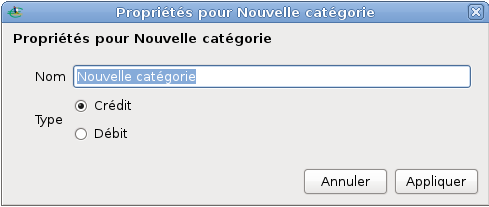
\includegraphics[scale=0.5]{image/screenshot/categories_new.png}}
% image entourée par un paragraphe ( picins)
\fi

La façon la plus immédiate pour créer une catégorie ou une sous-catégorie est de saisir son nom pendant la création d'une nouvelle opération dans l'onglet des comptes (voir la section \vref{transactions-fillcombo}, \menu{Nouveau tiers, catégorie ou imputation budgétaire}) ; mais vous pouvez aussi en créer ici, en cliquant sur l'outil \menu{Nouvelle catégorie} ou \menu{Nouvelle sous-catégorie}. Une boîte de dialogue s'ouvre ; suivant le cas, renseignez le nom de la catégorie et cochez si elle contiendra des crédits ou des débits, ou renseignez uniquement le nom de la sous-catégorie, puis validez.

% espace pour changement de thème
\vspacepdf{5mm}
L'outil \menu{Nouvelle sous-catégorie}\label{categories-newsub} de la barre d'outils ne devient actif que lorsqu'une catégorie est sélectionnée dans la liste.

\ifIllustration
% saut de page pour titre solidaire
\newpage
% espace après image entourée
\vspacehevea{5mm}
\fi


\section{Modification d'une catégorie ou d'une sous-catégorie\label{categories-modify}}


Pour modifier une catégorie ou une sous-catégorie, procédez comme suit :
% espace avant image 5mm
\vspacepdf{3mm}

\begin{enumerate}	
	\ifIllustration
	% image entourée par un paragraphe ( picins)
	% Pas de référence à l'illustration car erreur de numéro de figure avec picins.
	\pichskip{8mm}
	% supprimé car en html les figures entourées ne sont pas numérotées, et la numérotation des figures centrées décalée par rapport au pdf
%	\piccaption{Modification d'une catégorie}
	\label{categories-infos-img}
	\parpic[r]{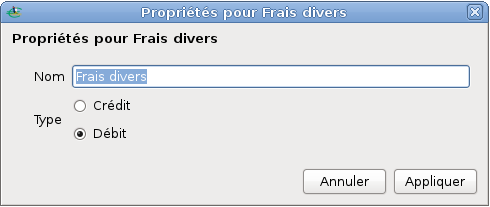
\includegraphics[scale=0.51]{image/screenshot/categories_infos}}
	% image entourée par un paragraphe ( picins)
	\fi
	 \item sélectionnez sa ligne ;
	 \item cliquez sur l'outil \menu{Éditer} dans la barre d'outils, ou sélectionnez \menu{Éditer la catégorie sélectionnée} ou \menu{Éditer la sous-catégorie sélectionnée} dans le menu contextuel accessible par un  clic-droit ;
	 \item une boîte de dialogue s'affiche : modifiez son nom et, seulement pour les catégories, son type (crédit ou débit) ;
	 \item validez.
\end{enumerate}


\textbf{Note} : la sous-catégorie \menu{Pas de sous-catégorie} est créée automatiquement par Grisbi ; vous ne pouvez pas la modifier.


\section{Transfert d'opérations dans une autre sous-catégorie\label{categories-transfer}}

Vous pouvez \indexword{transférer des opérations dans une autre sous-catégorie}\index{sous-catégories !transfert d'opérations} ayant pour point commun soit le tiers, soit la remarque, soit les deux ; pour cela, procédez comme suit :
% espace avant image 5mm
\vspacepdf{3mm}

\begin{enumerate}
	\ifIllustration
	% image entourée par un paragraphe ( picins)
	% Pas de référence à l'illustration car erreur de numéro de figure avec picins.
	\pichskip{8mm}
	% supprimé car en html les figures entourées ne sont pas numérotées, et la numérotation des figures centrées décalée par rapport au pdf
	%\piccaption{Transfert d'opérations identiques dans une autre sous-catégorie}
	\label{categories_transfer-img}
	\parpic[r]{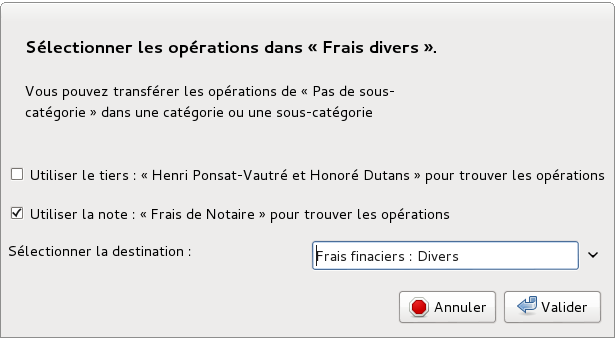
\includegraphics[scale=0.51]{image/screenshot/categories_transfer}}
	% image entourée par un paragraphe ( picins)
	\fi
	
	 \item sélectionnez la ligne de l'opération concernée ;
	 \item sélectionnez \menu{Transférer des opérations identiques dans une autre sous-catégorie}, dans le menu contextuel accessible par un  clic-droit ;
	 \item une boîte de dialogue s'affiche ; cochez l'une des deux cases \menu{Utiliser le tiers\ldots{ }} et \menu{Utiliser la note\ldots{ }} ou les deux selon votre besoin ;
	 \item renseignez le champ libellé \menu{Sélectionner la destination}, ou choisissez une catégorie et une sous-catégorie dans la liste déroulante ;
	 \item validez.
\end{enumerate}

\textbf{Note} : la saisie du champ de libellé \menu{Sélectionner la destination} bénéficie de la fonction d'\indexword{auto-complètement}\index{champ de saisie !auto-complètement}.

\ifIllustration
% espace après image entourée
\vspacehevea{15mm}
\fi

\section{Gestion des sous-catégories\label{categories-management}}


Vous pouvez modifier l'organisation de vos sous-catégories en \indexword{déplaçant le contenu d'une sous-catégorie}\index{sous-catégories !déplacement d'opération} vers une autre ou vers une nouvelle catégorie. Pour cela, sélectionnez une sous-catégorie, puis cliquez-droit et choisissez dans le menu contextuel \ifIllustration \refimage{categories-management-img} :
\else  :
\fi

\begin{itemize}
	 \item pour une sous-catégorie \menu{Pas de sous-catégorie} non vide : sélectionnez  \menu{Transférer les opérations dans une autre sous-catégorie} : une fenêtre s'affiche ; sélectionnez la destination dans la liste déroulante, puis validez ;

	 \item pour les autres sous-catégories : sélectionnez \menu{Gérer les sous-catégories}, une fenêtre s'affiche ; sélectionnez l'action désirée  :
		\begin{itemize}
			 \item \menu{Transférer les opérations dans une catégorie ou une sous-catégorie} : sélectionnez la catégorie de destination dans la liste déroulante, puis validez,
			 \item \menu{Transférer \og nom de la sous-catégorie sélectionnée \fg{} dans une autre catégorie} : sélectionnez la catégorie de destination dans la liste déroulante, puis validez,
			 \item \menu{Convertir \og nom de la sous-catégorie sélectionnée \fg{} en nouvelle catégorie} : validez, la sous-catégorie est devenue une catégorie.
		\end{itemize}
\end{itemize}

\ifIllustration
% image centrée
\begin{figure}[htbp]
\begin{center}
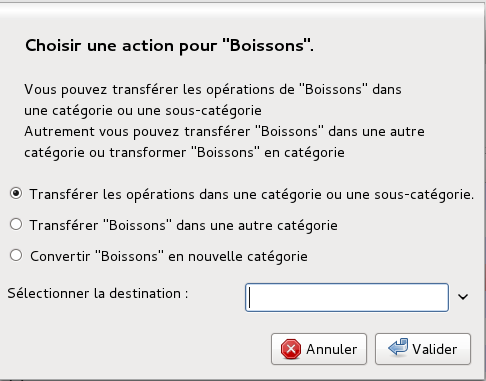
\includegraphics[scale=0.5]{image/screenshot/categories_management}
\end{center}
\caption{Gestion des sous-catégories}
\label{categories-management-img}
\end{figure}
% image centrée
\fi

%
\section{Suppression d'une catégorie ou d'une sous-catégorie\label{categories-delete}}


Pour supprimer une catégorie ou une sous-catégorie, procédez comme suit :
% espace avant image 5mm
\vspacepdf{3mm}

\begin{enumerate}
	\ifIllustration
	% image entourée par une liste (picins)
	% Pas de référence à l'illustration car erreur de numéro de figure avec picins.
	\pichskip{8mm}
	% supprimé car en html les figures entourées ne sont pas numérotées, et la numérotation des figures centrées décalée par rapport au pdf
	%\piccaption{Suppression d'une catégorie}
	\label{categories-delete-img}
	\parpic[r]{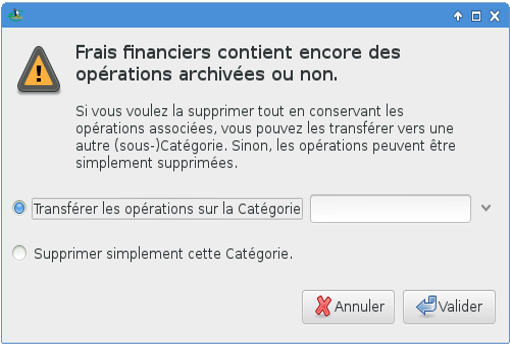
\includegraphics[scale=0.5]{image/screenshot/categories_delete}}
	% image entourée par une liste (picins)
	\fi
	 \item sélectionnez-la dans la liste ;
	 \item cliquez sur l'outil \menu{Supprimer} dans la barre d'outils ;
	 \item une  boîte de dialogue s'ouvre et vous propose soit de réaffecter les opérations de cette (sous-) catégorie vers une autre (sous-) catégorie, soit de la supprimer purement et simplement, y compris toutes ses opérations ;
	 \item faites votre choix puis validez.
\end{enumerate}


\ifIllustration
% espace après légende 10mm
\vspacepdf{9mm}
\fi

\strong{Attention} : la suppression d'une catégorie ou d'une sous-catégorie est \indexword{irréversible}\index{opération !irréversible} !

% espace avant Attention ou Note  : 5 mm
\vspacepdf{5mm}
\textbf{Note} : si la (sous-) catégorie que vous voulez supprimer ne contient aucune opération, aucune boîte de dialogue ne s'ouvrira et Grisbi la supprimera immédiatement.

\ifIllustration
% espace après image entourée
\vspacehevea{20mm}
\fi


\section{Import et export\label{categories-importexport} }


Grisbi vous permet d'importer ou d'exporter les catégories d'un fichier de comptes, ce qui peut éviter de recréer tout un ensemble de catégories si on peut le trouver ailleurs déjà fait.


\subsection{Import d'une liste de (sous-) catégories\label{categories-importexport-import} }

Pour \indexword{importer une liste de (sous-) catégories}\index{catégories !import}\index{sous-catégories !import}, procédez comme suit :

\begin{enumerate}
	 \item cliquez sur l'outil \menu{Importer} dans la barre d'outils : une fenêtre de gestionnaire de fichiers s'affiche ;
	 \item choisissez le répertoire et le nom du fichier à importer, dont l'\indexword{extension} doit être \file{.cgsb}\index{extension !.cgsb}\index{cgsb} ;
	 \item cliquez sur le bouton \menu{Ouvrir} ; une boîte de dialogue vous demande de choisir entre deux options :
		    \begin{itemize}
			      \item fusion des catégories importées avec celles de votre fichier de comptes en cours d'utilisation (bouton \menu{Valider}),
			      \item remplacement des catégories de votre fichier de comptes en cours d'utilisation par les catégories importées (bouton \menu{Remplacer l'existant}) ;
		     \end{itemize}
	 \item cliquez sur le bouton de votre choix ; les nouvelles catégories sont enregistrées dans votre fichier de comptes, en plus de celles qui étaient déjà présentes.
\end{enumerate}

\strong{Attention} : d'une manière générale, il est déconseillé d'avoir des accents ou des espaces dans les noms des répertoires et fichiers utilisés par Grisbi. Si c'est le cas, renommez-les maintenant. Par exemple, les espaces peuvent être remplacées par des tirets bas (\_).

% espace après Attention ou Note  : 5 mm
\vspacepdf{5mm}
Quelle que soit l'option choisie, il vous appartient ensuite de supprimer une à une toutes les catégories que vous ne voulez pas garder, ou d'en créer de nouvelles.

% espace avant Attention ou Note  : 5 mm
\vspacepdf{5mm}
\textbf{Note} : si vous commencez un fichier de comptes neuf, vous aurez avantage à supprimer les catégories existantes par défaut avant d'importer une autre liste.


\subsection{Export de vos (sous-) catégories\label{categories-importexport-export} }

Pour \indexword{exporter la liste de vos (sous-) catégories}\index{catégories !export}\index{sous-catégories !export}, procédez comme suit :

\begin{enumerate}
	 \item cliquez sur l'outil \menu{Exporter} dans la barre d'outils : une fenêtre de gestionnaire de fichiers s'affiche ;
	 \item saisissez le nom du fichier à exporter, dont l'\indexword{extension} sera \file{.cgsb}\index{extension !.cgsb}\index{cgsb} ;
	 \item choisissez son répertoire de destination ;
	 \item cliquez sur le bouton \menu{Enregistrer}.
\end{enumerate}

% espace avant Attention ou Note  : 5 mm
\strong{Attention} : d'une manière générale, il est déconseillé d'avoir des accents ou des espaces dans les noms des répertoires et fichiers utilisés par Grisbi. Si c'est le cas, renommez-les maintenant. Par exemple, les espaces peuvent être remplacées par des tirets bas (\_).

%
%
%%\subsection{Format des fichiers de catégories}
%%
%%Ces fichiers sont enregistrés au format \file{XML}, comme le fichier de comptes.
%%La structure du fichier est identique à celle du fichier de comptes, section
%%\file{Categories} (voir l'annexe \vref{xml-categories}).
\myclearemptydoublepage

%%%%%%%%%%%%%%%%%%%%%%%%%%%%%%%%%%%%%%%%%%%%%%%%%%%%%%%%%%%%%%%%%
% Contents : The budgetary lines chapter
% $Id : grisbi-manuel-budgetlines.tex, v 0.4 2002/10/27 Daniel Cartron
% $Id : grisbi-manuel-budgetlines.tex, v 0.5.0 2004/06/01 Loic Breilloux
% some of its content was in tips chapter  : 
% $Id : grisbi-manuel-tips.tex, v 0.4 2002/10/27 Daniel Cartron
% $Id : grisbi-manuel-budgetlines.tex, v 0.6.0 2011/11/17 Jean-Luc Duflot
% some of its content was in tips chapter  :
% $Id : grisbi-manuel-tips.tex, v 0.5.0 2004/06/01 Loic Breilloux
% $Id : grisbi-manuel-budgetlines.tex, v 0.8.9 2012/04/27 Jean-Luc Duflot
% $Id : grisbi-manuel-budgetlines.tex, v 1.0 2014/02/12 Jean-Luc Duflot
%%%%%%%%%%%%%%%%%%%%%%%%%%%%%%%%%%%%%%%%%%%%%%%%%%%%%%%%%%%%%%%%%

\chapter{Imputations budgétaires\label{budgetarylines}}

Grisbi vous permet de classer vos opérations selon des axes budgétaires, en plus du classement dans des catégories. 

Une imputation budgétaire définit la fonction de l'opération : il s'agit du travail, de la vie courante, des vacances, d'un projet d'aménagement, etc. Tandis qu'une imputation comptable, nommée \menu{Catégorie} dans Grisbi, définit la nature de  l'opération : frais de transport, habillement, etc. D'une autre manière, \emph{pourquoi} et \emph{quoi}\ldots{ } Voir aussi le chapitre \vref{categories}, \menu{Catégories}.

%espace pour changement de thème
\vspacepdf{5mm}
Cette information complémentaire à celle de l'imputation comptable vous permet de mieux appréhender vos flux financiers, sans pour autant vous surcharger en catégories et sous-catégories. Prenons un exemple : vous voulez savoir combien vous ont coûté vos vacances. Dans Grisbi vous allez simplement créer une imputation budgétaire \menu{Vacances} ; chacune de vos dépenses d'alimentation sera affectée à une catégorie (imputation comptable), par exemple \menu{Alimentation : Epicerie}, ET à l'imputation budgétaire \menu{Vacances}. Vous pouvez même aller plus loin et créer des sous-imputations budgétaires \menu{Vacances :été} et \menu{Vacances :hiver}. Ensuite, dans l'onglet \menu{Imputations budgétaires}, vous verrez d'un seul coup d'\oe il combien vous ont coûté vos vacances, éventuellement avec un sous-total par vacances d'été et d'hiver. Et bientôt vous pourrez utiliser ces informations pour votre  budget.

%espace pour changement de thème
\vspacepdf{5mm}
Si vous préférez vous passer des imputations budgétaires, désactivez leur affichage dans le formulaire de saisie des opérations grâce au menu \menu{Édition - Préférences} (voir la section \vref{setup-form-content}, \menu{Contenu}) et dans la liste des opérations grâce au même menu (voir la section \vref{setup-operations-cells}, \menu{Cellules de la liste des opérations}), et vous n'aurez plus  à vous en occuper. De toutes façons et par rapport à notre exemple, la liste des catégories intégrée par défaut dans Grisbi contient déjà la catégorie \menu{Vacances}.

% espace pour changement de thème
\vspacepdf{5mm}
Après son installation, Grisbi ne propose pas par défaut de liste d'imputations budgétaires, et il n'y a pas de champ \menu{imputation budgétaire} dans le formulaire de saisie des opérations. Pour pouvoir utiliser cette fonctionnalité, vous devrez \indexword{activer l'affichage de l'imputation budgétaire}\index{imputations budgétaires !activation} dans ce formulaire au moyen du  menu \menu{Édition - Préférences } (voir la section \vref{setup-form-content}, \menu{Contenu}) et dans la liste des opérations dans le même menu (voir la section \vref{setup-operations-cells}, \menu{Cellules de la liste des opérations}). Vous pouvez aussi vous servir de votre liste de catégories comme base pour établir votre liste d'imputations budgétaires (voir la section \vref{budgetarylines-importexport-importCategories}, \menu{Import d'une liste de (sous-) catégories}).

 % espace avant Attention ou Note  : 5 mm
\vspacepdf{5mm}
\textbf{Note} : si vous utilisez les imputations budgétaires, toutes vos opérations devraient être affectées à une imputation budgétaire \emph{et} à une sous-imputation budgétaire, pour deux raisons : elles pourront ainsi être bien classées, donc facilement gérées, et de plus, si elles ne sont pas affectées, elles pourraient ne pas être prises en compte dans les budgets prévisionnels.

% espace avant Attention ou Note  : 5 mm
\vspacepdf{5mm}
\textbf{Note} : Il est donc conseillé de bien étudier votre liste d'imputations budgétaires, pour éviter d'avoir à la modifier fréquemment pour cause d'incohérences ou de redondances. Si vous avez vraiment des opérations inclassables, créez une imputation ou des sous-imputations \og Divers \fg{}, mais n'abusez pas de leur emploi.

% espace pour changement de thème
\vspacepdf{5mm}
L'onglet \menu{Imputations budgétaires} sert à gérer toutes les imputations et sous-imputations budgétaires de votre fichier de comptes. 

Pour avoir accès à la gestion des imputations budgétaires, sélectionnez \menu{Imputations budgétaires} dans le panneau de navigation ou avec la barre d'information (voir le chapitre \vref{home}, \menu{Accueil}).

La barre d'information affiche, à gauche, le nom de l'imputation et de la sous-imputation budgétaire sélectionnées dans le pavé des détails et, complètement à droite, le solde des opérations affectées.

Le pavé des détails affiche deux éléments :
\begin{itemize}
	 \item la barre d'outils ;
	 \item la liste des imputations budgétaires.
\end{itemize}


\section{Barre d'outils\label{budgetarylines-functions}}


La barre d'outils des imputations budgétaires présente les fonctions suivantes :

\begin{itemize}
	 \item \menu{Nouvelle imputation} : ouvre une fenêtre pour créer une nouvelle imputation budgétaire ;
	 \item \menu{Nouvelle sous-imputation} : ouvre une fenêtre pour créer une nouvelle sous-imputation budgétaire ;
	 \item \menu{Importer} : permet d'importer une liste d'imputations budgétaires contenue dans un fichier ;
	 \item \menu{Exporter} : permet d'exporter une liste d'imputations budgétaires dans un fichier ;
	 \item \menu{Supprimer} : supprime l'imputation ou la sous-imputation budgétaire sélectionnée ;
	 \item \menu{Éditer} : ouvre une fenêtre pour modifier le nom de l'imputation ou de la sous-imputation budgétaire sélectionnée ;
	 \item \menu{Affichage} : ouvre un menu déroulant pour afficher la liste des 	imputations, avec ou sans leurs sous-imputations budgétaires.
\end{itemize}

% FONCTION SUPPRIMÉE La barre d'outils peut être déplacée dans l'écran en cliquant sur sa poignée (petit rectangle vertical à gauche de la barre) et en la déplaçant. Pour la réattacher à son emplacement d'origine dans le pavé des détails, la remettre en haut de la fenêtre, le haut de la poignée sur le petit trait qui visualise sa place d'origine.


\section{Liste des imputations budgétaires\label{budgetarylines-list}}


La liste des imputations et sous-imputations budgétaires s'affiche dans le panneau des 
\ifIllustration détails\refimage{budgetarylines-list-img}.
\else détails.
\fi

\ifIllustration
% image centrée
\begin{figure}[htbp]
\begin{center}
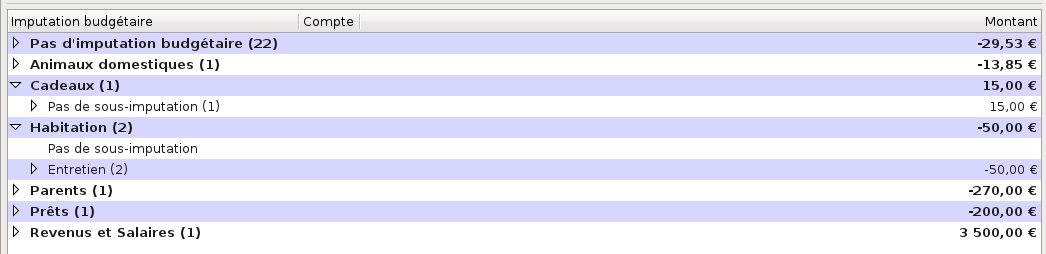
\includegraphics[scale=0.5]{image/screenshot/budgetarylines_list}
\end{center}
\caption{Liste des imputations et des sous-imputations budgétaires}
\label{budgetarylines-list-img}
\end{figure}
% image centrée
\fi

Elle affiche en haut la barre des libellés des colonnes ; ses champs d'affichage sont les suivants :
\begin{itemize}
	 \item le nom de l'imputation ou de la sous-imputation budgétaire ;
	 \item le compte concerné ;
	 \item le montant total des opérations affectées aux imputations et sous-imputations budgétaires, et le montant de chaque opération affectée à ces imputations et sous-imputations budgétaires si leurs lignes sont déroulées.
\end{itemize}

Vous pouvez déplacer la liste des imputations budgétaires vers le haut ou vers le bas avec la molette de la souris, ou bien avec la souris et l'ascenseur vertical. Le déplacement éventuel vers la gauche ou la droite se fait avec la souris et l'ascenseur horizontal.

Pour  afficher les sous-imputations d'une imputation budgétaire, cliquez sur le petit triangle à gauche de son nom, ou bien double-cliquez sur sa ligne ;
% ou bien sélectionnez-la et appuyez sur la barre d'espace (non fonctionnel) 
 cela affiche le libellé  de toutes les sous-imputations, et éventuellement, en première position, \indexword{\menu{Pas de sous-imputation}}\index{sous-imputations budgétaires !pas de sous-imputation}.
 
\textbf{Note} : ces triangles peuvent être remplacés, en fonction du thème de l'environnement de bureau ou du gestionnaire de fenêtres que vous utilisez, par d'autres caractères tels que +, -, >, <, etc. 

%le seul moyen de dérouler la liste est de cliquer sur le petit triangle. il devrait y avoir un moyen avec le clavier, comme ça existe avec le formulaire de saisie, où l'on peut utiliser la barre d'espace pour le moyen de paiement, ou la touche flèche bas pour la catégorie...

% espace pour changement de thème
\vspacepdf{5mm}
Vous pouvez afficher plusieurs \indexword{imputations budgétaires déroulées}\index{imputations budgétaires !déroulées}. Pour ne plus les afficher, \indexword{enroulez les imputations budgétaires}\index{imputations budgétaires !enroulées} en cliquant sur le petit triangle à gauche de leur nom, ou bien double-cliquez sur leur ligne. Vous pouvez aussi dérouler ou enrouler toutes les imputations budgétaires de la liste, en cliquant sur l'outil \menu{Affichage}\index{affichage !imputations budgétaires} dans la barre d'outils et en choisissant \menu{Vue des imputations et des sous-imputations}. Pour afficher seulement les imputations, cliquez sur l'outil \menu{Affichage} dans la barre d'outils et choisissez \menu{Vue des imputations uniquement}.

Les imputations et sous-imputations de votre fichier de comptes sont affichées par ordre alphabétique, avec deux exceptions : la première imputation affichée est toujours l'imputation de libellé \indexword{\menu{Pas d'imputation}}\index{imputations budgétaires !pas d'imputation}, qui reçoit toutes les opérations dont l'imputation n'est pas définie, et, à l'intérieur d'une imputation, la première sous-imputation affichée est toujours la sous-imputation de libellé \indexword{\menu{Pas de sous-imputation}} \index{sous-imputations budgétaires !pas de sous-imputation}, qui reçoit toutes les opérations dont la sous-imputation n'est pas définie.

Le nombre d'opérations affectées à chaque imputation ou sous-imputation budgétaire s'affiche, entre parenthèses, à la suite de son nom, et le montant total des opérations affectées à ces imputations ou sous-imputations budgétaires s'affiche dans la colonne \menu{Montant}, à droite sur la même ligne. 

% Bogue connu  : en cliquant sur une ligne de catégories, la barre d'information devrait afficher le total, mais n'affiche que 0.

\ifIllustration
\else
% espace avant Attention ou Note  : 5 mm
\vspacepdf{5mm}
\fi

\textbf{Note} : vous pouvez configurer la \indexword{devise des totaux}\index{devise !totaux} de toutes les (sous-) imputations budgétaires dans le menu \menu{Édition - Préférences} (voir la section \vref{setup-display-third-currencies}, \menu{Devises des totaux}).


\section{Sélection d'une (sous-) imputation budgétaire\label{budgetarylines-selection}}


Pour sélectionner une imputation ou une sous-imputation budgétaire, vous avez deux moyens :

\begin{itemize}
	 \item cliquez sur sa ligne ;
	 \item déplacez la sélection avec les touches du clavier \key{Flèche Haut}, \key{Flèche Bas}, \key{Page Haut} ou \key{Page Bas}.
\end{itemize}

Le nom de l'imputation ou sous-imputation budgétaire apparaît alors sur fond rose{\couleur}.

% espace pour changement de thème
\vspacepdf{5mm}
Un menu contextuel est disponible par un clic-droit sur la liste des imputations budgétaires ; selon la ligne sélectionnée, vous pouvez exécuter les fonctions suivantes :

\begin{itemize}
	 \item pour une imputation budgétaire : \menu{Éditer l'imputation sélectionnée} ;
	 \item pour l'imputation budgétaire \menu{Pas de sous-imputation} :
		\begin{itemize}
			 \item si elle est vide :\menu{Éditer l'imputation sélectionnée},
			 \item si elle contient des opérations : \menu{Transférer les opérations dans une autre sous-imputation},
		\end{itemize}
	 \item pour	une sous-imputation quelconque :	
		\begin{itemize}
			 \item \menu{Éditer la sous-imputation sélectionnée},
			 \item \menu{Gérer les sous-imputations},			 
		\end{itemize}		
	 \item pour une opération quelconque : \menu{Transférer des opérations identiques dans une autre sous-imputation}.	
\end{itemize}


\section{Les opérations d'une (sous-) imputation budgétaire\label{budgetarylines-transactions}}


Une ligne de libellé \menu{Pas de sous-imputation} se comporte exactement comme une ligne de sous-imputation budgétaire.

Pour afficher les opérations, cliquez sur le petit triangle à gauche du libellé  \menu{Pas de sous-imputation} ou celui d'une sous-imputation, ou bien double-cliquez sur sa ligne,
% ou bien sélectionnez-la et appuyez sur la barre d'espace (non fonctionnel),
 ce qui déroule la liste. Les opérations sont alors décrites sur une seule ligne, avec leur date, leur remarque éventuelle, le nom du compte concerné et leur montant.

\textbf{Note} : ces triangles peuvent être remplacés, en fonction du thème de l'environnement de bureau ou du gestionnaire de fenêtres que vous utilisez, par d'autres caractères tels que +, -, >, <, etc. 

%le seul moyen de dérouler la liste est de cliquer sur le petit triangle. il devrait y avoir un moyen avec le clavier, comme ça existe avec le formulaire de saisie, où l'on peut utiliser la barre d'espace pour le moyen de paiement, ou la touche flèche bas pour la catégorie...

% espace pour changement de thème
\vspacepdf{5mm}
Vous pouvez afficher plusieurs lignes de \indexword{sous-imputations budgétaires déroulées}\index{sous-imputations budgétaires !déroulées}. Pour ne plus les afficher, \indexword{enroulez les  opérations}\index{sous-imputations budgétaires !enroulées} d'une sous-imputation budgétaire en cliquant sur le petit triangle à gauche de son nom, ou bien double-cliquez sur leur ligne. Vous pouvez aussi dérouler ou enrouler toutes les opérations de toutes les imputations et sous-imputations budgétaires de la liste, en cliquant sur l'outil \menu{Affichage}\index{affichage !sous-imputations} dans la barre d'outils, et en faisant votre choix entre \menu{Vue des imputations uniquement}, \menu{Vue des imputations et sous-imputations} ou \menu{Vue complète}.

%espace pour changement de thème
\vspacepdf{5mm}
Vous pouvez \indexword{déplacer une opération}\index{sous-imputations budgétaires !déplacement d'opération} d'une sous-imputation vers une autre sous-imputation de la liste en sélectionnant cette opération et en faisant un glisser-déplacer sur la sous-imputation cible, exactement à l'endroit où son nom est entouré d'une bordure pointillée.

%espace pour changement de thème
\vspacepdf{5mm}
Un \indexword{double-clic} sur une ligne d'opération d'une imputation\index{imputations budgétaires !double-clic sur opération} ou d'une sous-imputation budgétaire\index{sous-imputations budgétaires !double-clic sur opération} ferme l'onglet \menu{Imputations budgétaires}, ouvre l'onglet \menu{Comptes} et le sous-onglet du compte contenant cette opération, sélectionne l'opération concernée et l'affiche dans le formulaire de saisie. De cette façon, cette opération peut être affichée et modifiée facilement.


\section{Création d'une (sous-) imputation budgétaire\label{budgetarylines-new}}


La création d'une imputation budgétaire au cours de la saisie d'une opération n'est possible que si le champ d'information a été créé préalablement dans le formulaire de saisie des opérations (voir la section \vref{setup-form}, \menu{Formulaire des opérations}).

\ifIllustration
% image entourée par un paragraphe ( picins)
% Pas de référence à l'illustration car erreur de numéro de figure avec picins.
% supprimé car en html les figures entourées ne sont pas numérotées, et la numérotation des figures centrées décalée par rapport au pdf
%\piccaption{Création d'une imputation budgétaire}
\label{budgetarylines-new-img}
\parpic[r]{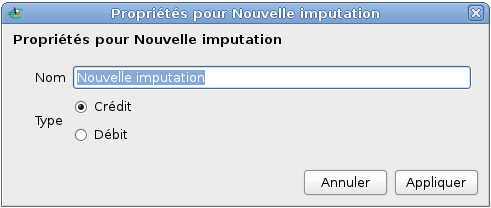
\includegraphics[scale=0.5]{image/screenshot/budgetarylines_new}}
% image entourée par un paragraphe ( picins)
\fi

\noindent La façon la plus immédiate pour créer une imputation ou une sous-imputation budgétaire est de saisir son nom au cours de la création d'une nouvelle opération dans l'onglet des comptes (voir la section \vref{transactions-fillcombo}, \menu{Nouveau tiers, catégorie ou imputation budgétaire}) ; mais vous pouvez aussi en créer ici, en cliquant sur l'outil \menu{Nouvelle imputation} ou \menu{Nouvelle sous-imputation}. Une boîte de dialogue s'ouvre ; suivant le cas, renseignez le nom de l'imputation et cochez si elle contiendra des crédits ou des débits, ou renseignez uniquement le nom de la sous-imputation, puis validez.

% espace pour changement de thème
\vspacepdf{5mm}
L'outil \menu{Nouvelle sous-imputation}\label{budgetarylines-newsub} de la barre d'outils ne devient actif que lorsqu'une imputation budgétaire est sélectionnée dans la liste.

\ifIllustration
% espace après image entourée
\vspacehevea{5mm}
\fi


\section{Modification d'une (sous-) imputation budgétaire\label{budgetarylines-modify}}


Pour modifier une imputation ou une sous-imputation budgétaire, procédez comme suit :
% espace avant image 5mm
\vspacepdf{3mm}

\begin{enumerate}
	\ifIllustration
	% image entourée par un paragraphe ( picins)
	% Pas de référence à l'illustration car erreur de numéro de figure avec picins.
	\pichskip{10mm}
	% supprimé car en html les figures entourées ne sont pas numérotées, et la numérotation des figures centrées décalée par rapport au pdf
	%\piccaption{Modification d'une imputation budgétaire}
	\label{budgetarylines-infos-img}
	\parpic[r]{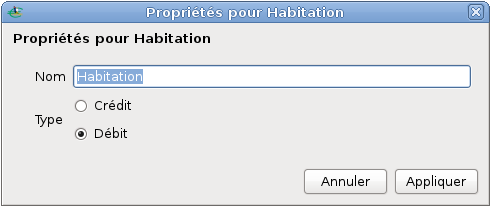
\includegraphics[scale=0.51]{image/screenshot/budgetarylines_infos}}
	% image entourée par un paragraphe ( picins)
	\fi
	 \item sélectionnez sa ligne ;
	 \item cliquez sur l'outil \menu{Éditer} dans la barre d'outils, ou sélectionnez \menu{Éditer l'imputation sélectionnée} ou \menu{Éditer la sous-imputation sélectionnée} dans le menu contextuel accessible par un  clic-droit ;
	 \item une boîte de dialogue s'ouvre : modifiez son nom et, uniquement pour les imputations, son type (crédit ou débit) ;
	 \item validez.
\end{enumerate}

\ifIllustration
% espace après inage entourée
\vspacehevea{6mm}
\fi

\section{Transfert d'opérations dans une autre sous-imputation\label{budgetarylines-transfer}}


Vous pouvez \indexword{transférer des opérations dans une autre sous-imputation}\index{sous-imputations budgétaires !transfert d'opérations} ayant pour point commun soit le tiers, soit la remarque, soit les deux ; pour cela, procédez comme suit :
% espace avant image 5mm
\vspacepdf{3mm}

% Pas de référence à l'illustration car erreur de numéro de figure avec picins.
\begin{enumerate}
	% image entourée par un paragraphe ( picins)
	\ifIllustration
	\pichskip{10mm}
	% supprimé car en html les figures entourées ne sont pas numérotées, et la numérotation des figures centrées décalée par rapport au pdf
	%\piccaption{Transfert d'opérations identiques dans une autre sous-imputation}
	\label{budgetarylines_transfer-img}
	\parpic[r]{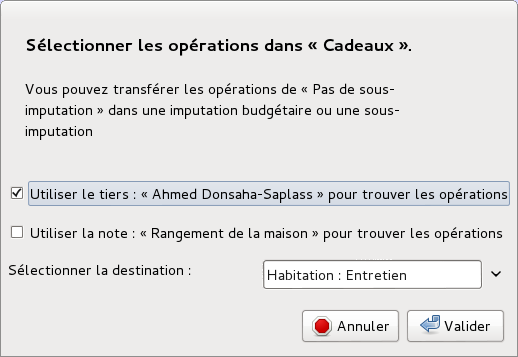
\includegraphics[scale=0.51]{image/screenshot/budgetarylines_transfer}}
	\fi
	% image entourée par un paragraphe ( picins)
	 \item sélectionnez la ligne de l'opération concernée ;
	 \item sélectionnez \menu{Transférer des opérations identiques dans une autre sous-imputa\dash tion}, dans le menu contextuel accessible par un  clic-droit ;
	 \item une boîte de dialogue s'affiche ; cochez l'une des deux cases \menu{Utiliser le tiers\ldots{ }} et \menu{Utiliser la note\ldots{ }} ou les deux selon votre besoin ;
	 \item renseignez le champ libellé \menu{Sélectionner la destination}, ou choisissez une imputation et une sous-imputation dans la liste déroulante ;
	 \item validez.
\end{enumerate}

\textbf{Note} : la saisie du champ libellé \menu{Sélectionner la destination} bénéficie de la fonction d'\indexword{auto-complètement}\index{champ de saisie !auto-complètement}.

\ifIllustration
% espace après image entourée
\vspacehevea{18mm}
\fi


\section{Gestion des sous-imputations budgétaires\label{budgetarylines-management}}


Vous pouvez modifier l'organisation de vos sous-imputations budgétaires en \indexword{déplaçant le contenu d'une sous-imputation}\index{sous-imputations budgétaires !déplacement d'opération} vers une autre ou vers une nouvelle imputation. Pour cela, sélectionnez une sous-imputation, puis cliquez-droit et choisissez dans le menu contextuel : 


\begin{itemize}
	 \item pour la sous-imputation \menu{Pas de sous-imputation} : sélectionnez \menu{Transférer les opérations dans une autre sous-imputation} : une fenêtre s'affiche ; sélectionnez la destination dans la liste déroulante, puis validez ;

	 \item pour les autres sous-imputations : sélectionnez \menu{Gérer les sous-imputations}, une fenêtre s'affiche ; sélectionnez l'action désirée \ifIllustration \refimage{budgetarylines-management-img} :
	 \else  :
	 \fi
		\begin{itemize}
			 \item \menu{Transférer les opérations dans une imputation ou une sous-imputation} : sélectionnez l'imputation de destination dans la liste déroulante, puis validez,
			 \item \menu{Transférer \og nom de la sous-imputation sélectionnée \fg{} dans une autre imputation} : sélectionnez l'imputation de destination dans la liste déroulante, puis validez,
			 \item \menu{Convertir \og nom de la sous-imputation sélectionnée \fg{} en nouvelle imputation} : validez, la sous-imputation est devenue une imputation.
		\end{itemize}
\end{itemize}

\ifIllustration
% image centrée
\begin{figure}[hbp]
\begin{center}
\includegraphics[scale=0.48]{image/screenshot/budgetarylines_management}
\end{center}
\caption{Gestion des sous-imputations budgétaires}
\label{budgetarylines-management-img}
\end{figure}
% image centrée
\fi


\section{Suppression d'une (sous-) imputation budgétaire\label{budgetarylines-delete}}


Pour supprimer une imputation ou une sous-imputation budgétaire, procédez comme suit :
% espace avant image 5mm
\vspacepdf{3mm}

\begin{enumerate}
	\ifIllustration
	% image entourée par une liste (picins)
	% Pas de référence à l'illustration car erreur de numéro de figure avec picins.
	\pichskip{11mm}
	% supprimé car en html les figures entourées ne sont pas numérotées, et la numérotation des figures centrées décalée par rapport au pdf
	%\piccaption{Suppression d'une sous-imputation budgétaire}
	\label{budgetarylines-delete-img}
	\parpic[r]{\includegraphics[scale=0.5]{image/screenshot/budgetarylines_delete}}
	% image entourée par une liste (picins)
	\fi
	
	 \item sélectionnez-la dans la liste ;
	 \item cliquez sur l'outil \menu{Supprimer} dans la barre d'outils ;
	 \item une  boîte de dialogue s'ouvre et vous propose soit de ré-affecter les opérations de cette (sous-) imputation vers une autre (sous-) imputation budgétaire, soit de la supprimer purement et simplement, y compris toutes ses opérations ; 
	 \item faites votre choix puis validez.
\end{enumerate}

\strong{Attention} : la suppression d'une imputation ou d'une sous-imputation budgétaire est \indexword{irréversible}\index{opération !irréversible} ! 

% espace avant Attention ou Note  : 5 mm
\vspacepdf{5mm}
\textbf{Note} : si la (sous-) imputation budgétaire que vous voulez supprimer ne contient aucune opération, aucune boîte de dialogue ne s'ouvrira et Grisbi la supprimera immédiatement.

\ifIllustration
% espace après inage entourée
\vspacehevea{3mm}
\fi


\section{Import et export\label{budgetarylines-importexport}}


Grisbi vous permet d'importer ou d'exporter les imputations budgétaires d'un fichier de comptes, ce qui peut éviter de recréer tout un ensemble d'imputations budgétaires si on peut le trouver ailleurs déjà fait.


\subsection{Import d'une liste de (sous-) imputations budgétaires\label{budgetarylines-importexport-import} }

Pour \indexword{importer une liste de (sous-) imputations budgétaires}\index{imputations budgétaires !import}\index{sous-imputations budgétaires !import}, procédez comme suit :

\begin{enumerate}
	 \item cliquez sur l'outil \menu{Importer} dans la barre d'outils : une fenêtre de gestionnaire de fichiers s'affiche ;
	 \item choisissez le répertoire et le nom du fichier à importer, dont l'\indexword{extension} doit être \file{.igsb}\index{extension !.igsb} ;
	 \item cliquez sur le bouton \menu{Ouvrir} ; 
	 \item une boîte de dialogue vous informe, éventuellement, que ce fichier contient déjà des opérations, et que sa liste d'imputations budgétaires et celle de votre fichier de comptes en cours seront fusionnées. Si cela vous convient, validez par le bouton \menu{Valider}.
\end{enumerate}

% espace avant Attention ou Note  : 5 mm
\vspacepdf{5mm}
\strong{Attention} : d'une manière générale, il est déconseillé d'avoir des accents ou des espaces dans les noms des répertoires et fichiers utilisés par Grisbi. Si c'est le cas, renommez-les maintenant. Par exemple, les espaces peuvent être remplacées par des tirets bas (\_). 
% espace après Attention ou Note  : 5 mm
\vspacepdf{5mm}

Si vous avez validé, il vous appartient ensuite de supprimer une à une toutes les imputations budgétaires que vous ne voulez pas garder, ou d'en créer de nouvelles.

Si vous commencez un fichier de comptes neuf, vous aurez avantage à supprimer les imputations budgétaires existantes par défaut avant d'importer une autre liste.


\subsection{Import d'une liste de (sous-) catégories\label{budgetarylines-importexport-importCategories} }

Si vous voulez vous servir de votre liste de (sous-) catégories comme base pour établir votre liste d'imputations budgétaires, vous devez d'abord exporter votre liste de (sous-) catégories dans un fichier. Pour cela, reportez-vous à la section \vref{categories-importexport-export}, \menu{Export de vos (sous-) catégories}. 

Puis, pour \indexword{importer votre liste de (sous-) catégories}\index{catégories !import}\index{sous-catégories !import}, procédez comme suit : 

\begin{enumerate}
	 \item cliquez sur l'outil \menu{Importer} dans la barre d'outils : une fenêtre de gestionnaire de fichiers s'affiche ;
	 \item dans le coin en bas et à droite de la fenêtre, sélectionnez dans la liste déroulante \menu{Fichier des catégories Grisbi (*.cgsb}) ;
	 \item choisissez le répertoire et le nom du fichier à importer, dont l'\indexword{extension} doit être \file{.cgsb}\index{extension !.cgsb} ;
	 \item cliquez sur le bouton \menu{Ouvrir} ; 
	 \item une boîte de dialogue vous propose, soit de fusionner votre liste de catégories avec votre liste d'imputations budgétaires existantes, soit que votre liste de catégories remplace votre liste d'imputations budgétaires existantes ; dans le cas de la fusion, cliquez sur le bouton \menu{Valider}, sinon dans le cas du remplacement, cliquez sur le bouton \menu{Remplacer l'existant}.
\end{enumerate}


\subsection{Export de vos (sous-) imputations budgétaires\label{budgetarylines-importexport-budgetary}}

Pour \indexword{exporter la liste de vos (sous-) imputations budgétaires}\index{imputations budgétaires !export}\index{sous-imputations budgétaires !export}, procédez comme suit :

\begin{enumerate}
	 \item cliquez sur l'outil \menu{Exporter} dans la barre d'outils : une fenêtre de gestionnaire de fichiers s'affiche ;
	 \item saisissez le nom du fichier à exporter, dont l'\indexword{extension} sera \file{.igsb}\index{extension !.igsb} :
	 \item choisissez son répertoire de destination :
	 \item cliquez sur le bouton \menu{Enregistrer}.
\end{enumerate}

% espace avant Attention ou Note  : 5 mm
\vspacepdf{5mm}
\strong{Attention} : d'une manière générale, il est déconseillé d'avoir des accents ou des espaces dans les noms des répertoires et fichiers utilisés par Grisbi. Si c'est le cas, renommez-les maintenant. Par exemple, les espaces peuvent être remplacées par des tirets bas (\_). 


%\subsection{Format des fichiers d'imputations budgétaires}
%
%Ces fichiers sont enregistrés au format \file{XML}, comme le fichier de comptes.
%La structure du fichier est identique à celle du fichier de comptes, section
%\file{Imputations budgétaires} (voir l'annexe \vref{xml-budgetarylines})
\myclearemptydoublepage

%%%%%%%%%%%%%%%%%%%%%%%%%%%%%%%%%%%%%%%%%%%%%%%%%%%%%%%%%%%%%%%%%
% Contents : The financialyear chapter
% $Id : grisbi-manuel-financialyear.tex, v 0.6.0 2011/11/17 Jean-Luc Duflot
% some of its content was in tips chapter  : 
% $Id : grisbi-manuel-tips.tex, v 0.4 2002/10/27 Daniel Cartron
% $Id : grisbi-manuel-financialyear.tex, v 0.8.9 2012/04/27 Jean-Luc Duflot
% $Id : grisbi-manuel-financialyear.tex, v 1.0 2014/02/12 Jean-Luc Duflot
%%%%%%%%%%%%%%%%%%%%%%%%%%%%%%%%%%%%%%%%%%%%%%%%%%%%%%%%%%%%%%%%%

\chapter{Exercices\label{financialyear}}


Un exercice est une période d'une durée d'un an pour laquelle sont établies des prévisions financières ou sont dégagés des résultats financiers pour un agent économique (un individu, un ménage, une entreprise, un État, etc.).

Cette période ne correspond pas toujours à l'année civile. Le découpage du temps en exercices financiers implique, en matière de calcul des résultats, un certain nombre de régularisations avant de procéder à la clôture des comptes. Il arrive en effet que certains produits et charges enregistrés au cours de l'exercice concernent effectivement les exercices suivants et, réciproquement, que des produits et des charges relatifs à l'exercice en cours n'aient pas encore été enregistrés.

Vous pouvez utiliser les exercices si vous voulez distinguer vos opérations dans vos états, non par rapport à la date sous laquelle vous les enregistrez, mais par rapport à la période comptable à laquelle elles appartiennent.


\section{Exemples d'utilisation}


Prenons l'exemple d'un remboursement de Sécurité Sociale, qui intervient nécessairement avec un délai par rapport à la dépense. Si vous voulez faire un bilan objectif de vos dépenses de santé, il vous faudra le prendre en compte pendant la même année que la dépense, donc fausser la date de  remboursement, même s'il intervient l'année suivante. 

On peut aussi prendre l'exemple d'une facture téléphonique, souvent bimestrielle, couvrant la période du 11 décembre 2012 au 10 février 2013. Si vous enregistrez cette facture en 2013, la totalité de son montant sera affectée à cette année-là. Vous pouvez considérer que cela compense le déséquilibre induit par la facture de l'année précédente à la même époque, et que bon an mal an vos comptes sont à peu près bons.

La seule façon de procéder correctement est d'utiliser les exercices. La période courante d'un exercice est l'année civile, mais l'année scolaire peut être plus intéressante si vous êtes trésorier d'une association. Vous pouvez même faire des exercices mensuels, bien que comptablement ce soit une \emph{bizarrerie}.

Pour le remboursement de Sécurité Sociale, vous l'enregistrerez alors avec le même exercice que celui de la dépense, et votre état ou votre budget prendra en compte cette recette comme il le faut.

Pour la facture téléphonique, vous ventilerez celle-ci \emph{prorata temporis} (c'est-à-dire proportionnellement au temps). Pour simplifier, il est communément admis qu'une année se compose de 12 mois de 30 jours chacun. On a donc ici vingt jours sur l'exercice 2012, et quarante jours sur l'exercice 2013. Votre facture devra donc être ventilée en vingt soixantièmes sur l'exercice 2012, et quarante soixantièmes sur l'exercice 2013.


\section{Mise en place des exercices\label{financialyear-start}}


Avant de procéder à l'utilisation d'exercices, vous devez définir les aspects suivants :

\begin{itemize}
	\item la définition de l'exercice pour l'importation de fichiers de compte, dans le menu \menu{Édition - Préférences} : voir le paragraphe \vref{setup-general-import-financialyear}, \menu{Définition de l'exercice} ;	
	\item la détermination automatique de l'exercice dans le formulaire de saisie des opérations, dans le menu \menu{Édition - Préférences} : voir la section \vref{setup-form-behaviour}, \menu{Comportement} ;
	\item l'affichage du champ \menu{Exercice} dans le formulaire de saisie des opérations, dans le menu \menu{Édition - Préférences} : voir la section \vref{setup-form}, \menu{Formulaire des opérations} ;
	\item l'affichage du champ \menu{Exercice} dans la liste des opérations : voir le paragraphe \vref{transactions-list-fields}, \menu{Champs d'information et de saisie}.
\end{itemize}

% espace pour changement de thème
\vspacepdf{5mm}
Lors de la saisie d'une opération, vous pourrez alors, dans le champ \menu{Exercice} du formulaire de saisie, entrer l'exercice au clavier, ou le  choisir grâce à la liste déroulante commençant par \menu{Automatique}. Une fois l'opération validée, elle apparaîtra dans la liste des opérations avec son exercice, dans la cellule que vous avez choisie.

Vous pourrez aussi modifier l'ordre d'affichage des opérations par un \gls{tri} suivant les exercices ou les dates (voir le paragraphe \vref{transactions-list-sorts}, \menu{Tris}).


\section{Création, modification et suppression d'un exercice}


La création, la modification et la suppression d'un exercice se fait grâce au menu \menu{Édition - Préférences} (voir la section \vref{setup-resources-financialyear}, \menu{Exercices}).















\myclearemptydoublepage

%%%%%%%%%%%%%%%%%%%%%%%%%%%%%%%%%%%%%%%%%%%%%%%%%%%%%%%%%%%%%%%
% Contents : The credit simulator chapter
% $Id : grisbi-manuel-credit.tex, v 0.8.9 2012/04/27 Jean-Luc Duflot
% $Id : grisbi-manuel-credit.tex, v 1.0 2014/02/12 Jean-Luc Duflot
%%%%%%%%%%%%%%%%%%%%%%%%%%%%%%%%%%%%%%%%%%%%%%%%%%%%%%%%%%%%%%%%%


\chapter{Simulation de crédits\label{credit}}


L'onglet \menu{Simulateur de crédits} permet de simuler les différents aspects d'un ou de plusieurs crédits. Il affiche les différents paramètres d'une liste de crédits, calculés à partir du montant emprunté, du taux, des frais attachés et de durées comprises dans une plage de durées. Il calcule et affiche aussi le tableau d'amortissement d'un crédit d'une durée déterminée, sélectionné dans cette liste.

%espace pour changement de thème
\vspacepdf{5mm}
Pour avoir accès à la simulation de crédits, sélectionnez \menu{Simulateur de crédits} dans le panneau de navigation ou avec la barre d'information (voir le chapitre \vref{home}, \menu{Accueil}).

La barre d'information affiche, à gauche, le nom de cet onglet.

Le pavé des détails affiche deux éléments :
\begin{itemize}
	 \item la barre d'outils ;
	 \item la page \menu{Simulateur de crédits} ou \menu{Tableau d'amortissement}, selon le choix fait dans la barre d'outils.
\end{itemize}


\section{Barre d'outils\label{credit-functions}}


La barre d'outils du simulateur de crédits présente les fonctions suivantes  :

\begin{itemize}
	 \item \menu{Calculer} : ne s'affiche que si vous êtes dans la page \menu{Simulateur de crédits} ; elle lance le calcul d'une liste de crédits ; 
	 \item \menu{Amortissement} : ne s'affiche que si vous êtes dans la page \menu{Simulateur de crédits} ; cliquez dessus pour afficher la page  \menu{Tableau d'amortissement} ;
	 \item \menu{Crédits} : ne s'affiche que si vous êtes dans la page \menu{Amortissement} ; cliquez dessus pour afficher la page  \menu{Simulateur de crédits} ;
	 \item \menu{Imprimer} : ouvre la fenêtre de sélection de l'imprimante et de ses options ;
	 \item \menu{Exporter} : permet d'exporter dans un fichier le tableau affiché dans la page \menu{Simulateur de crédits} ou \menu{Amortissement}.
\end{itemize}

%espace pour changement de thème
\vspacepdf{5mm}
% FONCTION SUPPRIMÉE La barre d'outils peut être déplacée dans l'écran en cliquant sur sa poignée (petit rectangle vertical à gauche de la barre) et en la déplaçant. Pour la réattacher à son emplacement d'origine dans le pavé des détails, la remettre en haut de la fenêtre, le haut de la poignée sur le petit trait qui visualise sa place d'origine.

\ifIllustration
\else
% saut de page pour titre solidaire
\newpage
\fi


\section{Simulateur de crédits\label{credit-simulation}}


Pour afficher les détails du \menu{Simulateur de crédits}, sélectionnez son onglet dans le panneau de navigation ou avec la barre d'information (voir le chapitre \vref{home}, \menu{Accueil}), ou bien, s'il est déjà sélectionné, sélectionnez \menu{Crédits} dans la barre \ifIllustration d'outils\refimage{credit-simulation-img}.
\else d'outils.
\fi

\ifIllustration
% image centrée 
\begin{figure}[htb]
\begin{center}
\includegraphics[scale=0.5]{image/screenshot/credit_simulation}
\end{center}
\caption{Simulateur de crédits}
\label{credit-simulation-img}
\end{figure}
% image centrée
\fi
 
Le simulateur de crédits se compose de deux éléments :
\begin{itemize}
	 \item la définition du crédit ; 
	 \item la liste des crédits simulés.
\end{itemize}


\subsection{Définition du crédit\label{credit-simulation-definition}}

La \menu{Définition du crédit} s'affiche en haut du panneau des détails, sous la barre d'outils. Elle affiche et permet de définir les caractéristiques principales du crédit suivantes :

\begin{itemize}
	 \item le capital emprunté ; 
	 \item la devise du crédit ;
	 \item le taux d'intérêt annuel ;
	 \item la plage de durée du crédit ;
	 \item les frais, en pourcentage du capital emprunté ;
	 \item le type du taux appliqué.
\end{itemize}


\subsection{Liste des crédits simulés\label{credit-simulation-list}}

La liste des crédits simulés s'affiche en bas du panneau des détails, sous la  \menu{Définition du crédit}. Elle affiche les caractéristiques détaillées de tous les crédits dont la durée fait partie de la plage de durées choisie dans la définition du crédit. 

La liste affiche en haut la barre de libellés des colonnes. Vous pouvez \indexword{élargir ou rétrécir une colonne}\index{colonne !largeur} en cliquant sur le séparateur entre deux colonnes et en le déplaçant. 

%XXXXXX Ne fonctionne pas  : XXXXXX Pour rétablir la largeur des colonnes à leur valeur par défaut, sélectionnez le menu \menu{Affichage - Réinitialiser la largeur des colonnes}.
%XXXXXX Ne fonctionne pas  : XXXXXX

%espace pour changement de thème
\vspacepdf{5mm}
La liste des crédits simulés affiche autant de lignes qu'il y a de durées de crédits possibles dans la plage de durées choisie dans la définition du crédit. Ses champs d'affichage sont les suivants :

\begin{itemize}
	 \item \menu{Durée} ;
	 \item \menu{Nombre d'échéances} ;
	 \item \menu{Capital emprunté} ;
	 \item \menu{Taux d'intérêt annuel} ;
	 \item \menu{Montant de l'échéance hors frais} ;
	 \item \menu{Montant des frais} ;
	 \item \menu{Mensualité} ;
	 \item \menu{Coût total du crédit}.
\end{itemize}

% espace pour changement de thème
\vspacepdf{5mm}
Vous pouvez déplacer la liste des crédits vers le haut ou vers le bas avec la molette de la souris, ou bien avec la souris et l'ascenseur vertical. 

%XXXXXX Ne fonctionne pas  : XXXXXXLe déplacement éventuel vers la gauche ou la droite se fait avec la souris et l'ascenseur horizontal.XXXXXX Ne fonctionne pas  : XXXXXX

Chaque crédit est affiché sur une ligne. Pour une bonne lisibilité de l'affichage, Grisbi présente une alternance de couleurs de fond violet et blanc{\couleurs} à chaque ligne.

%espace pour changement de thème
\vspacepdf{5mm}
Pour sélectionner un crédit, vous avez deux moyens :
\begin{itemize}
	 \item cliquez sur une de ses lignes ;
	 \item déplacez la sélection avec les touches du clavier \key{Flèche Haut}, \key{Flèche Bas}.
\end{itemize}
La ligne apparaît alors sur fond rouge{\couleur}.

%espace pour changement de thème
\vspacepdf{5mm}
Un menu contextuel est disponible par un clic-droit sur une ligne, et propose les actions suivantes :
\begin{itemize}
	 \item \menu{Afficher le tableau d'amortissement} ;
	 \item \menu{Imprimer le tableau} ;
	 \item \menu{Exporter le tableau}.
\end{itemize}


\section{Tableau d'amortissement\label{credit-amortization}}


Pour afficher les détails des amortissements, sélectionnez \menu{Amortissement} dans la barre 
\ifIllustration d'outil\refimage{credit-amortization-img}.
\else d'outils.
\fi

\ifIllustration
% image centrée 
\begin{figure}[tbp]
\begin{center}
\includegraphics[scale=0.5]{image/screenshot/credit_amortization}
\end{center}
\caption{Tableau d'amortissement}
\label{credit-amortization-img}
\end{figure}
% image centrée
\fi

Le tableau d'amortissement se compose de deux éléments :
\begin{itemize}
	 \item la définition du crédit ; 
	 \item le tableau d'amortissement détaillé.
\end{itemize}


\subsection{Définition du crédit\label{credit-amortization-definition}}

La définition du crédit s'affiche en haut du panneau des détails, sous la barre d'outils. Elle affiche, \emph{mais ne permet pas de définir}, les caractéristiques principales du crédit suivantes :

\begin{itemize}
	 \item le montant emprunté ; 
	 \item le taux d'intérêt annuel ;
	 \item la durée du crédit.
\end{itemize}


\subsection{Tableau d'amortissement détaillé\label{credit-amortization-details}}

Le tableau d'amortissement détaillé s'affiche en bas du panneau des détails, sous la \menu{Définition du crédit}. Il affiche les caractéristiques détaillées de chaque échéance d'un crédit dont les caractéristiques principales sont affichées dans la définition du crédit juste au-dessus, et qui a été sélectionné dans la liste des crédits. 

Il affiche en haut la barre de libellés des colonnes. Vous pouvez \indexword{élargir ou rétrécir une colonne}\index{colonne !largeur} en cliquant sur le séparateur entre deux colonnes et en le déplaçant. 

%XXXXXX Ne fonctionne pas  : XXXXXX Pour rétablir la largeur des colonnes à leur valeur par défaut, sélectionnez le menu \menu{Affichage - Réinitialiser la largeur des colonnes}.
%XXXXXX Ne fonctionne pas  : XXXXXX

%espace pour changement de thème
\vspacepdf{5mm}
Le tableau d'amortissement affiche autant de lignes qu'il y a d'échéances dans le crédit choisi. Ses champs d'affichage sont les suivants :

\begin{itemize}
	 \item \menu{Numéro de l'échéance} ;
	 \item \menu{Capital restant dû} ;
	 \item \menu{Montant des intérêts} ;
	 \item \menu{Capital remboursé} ;
	 \item \menu{Montant des frais} ;
	 \item \menu{Mensualité}.
\end{itemize}

% espace pour changement de thème
\vspacepdf{5mm}
Vous pouvez déplacer la liste des échéances vers le haut ou vers le bas avec la molette de la souris, ou bien avec la souris et l'ascenseur vertical. 

%XXXXXX Ne fonctionne pas  : XXXXXX
%Le déplacement vers la gauche ou la droite se fait avec la souris et l'ascenseur horizontal.
%XXXXXX Ne fonctionne pas  : XXXXXX

Chaque échéance est affichée sur une ligne. Pour une bonne lisibilité de l'affichage, Grisbi présente une alternance de couleurs de fond violet et blanc{\couleurs} à chaque ligne.

%espace pour changement de thème
\vspacepdf{5mm}
Pour sélectionner une échéance, vous avez deux moyens :
\begin{itemize}
	 \item cliquez sur une de ses lignes ;
	 \item déplacez la sélection avec les touches du clavier \key{Flèche Haut}, \key{Flèche Bas}, \key{Page Haut}et \key{Page Bas}.
\end{itemize}
La ligne apparaît alors sur fond rouge{\couleur}.

%espace pour changement de thème
\vspacepdf{5mm}
Un menu contextuel est disponible par un clic-droit sur une ligne, et propose les actions suivantes :

\begin{itemize}
	 \item \menu{Afficher le simulateur de crédits} : affiche la zone de définition du crédit et la liste des crédits possibles ;
	 \item \menu{Imprimer le tableau} ;
	 \item \menu{Exporter le tableau}.
\end{itemize}


\section{Simulation d'un nouveau crédit\label{credit-new}}


Pour avoir accès à la simulation d'un nouveau crédit, cliquez sur \menu{Crédits} dans la barre d'outils (si cette fonction n'apparaît pas, c'est que le simulateur de crédits est déjà affiché).

% espace avant Attention ou Note  : 5 mm
\vspacepdf{5mm}
\textbf{Note} : À l'ouverture du simulateur de crédits, Grisbi affiche dans le pavé des détails les paramètres de définition du crédit et la liste des crédits générés lors d'une simulation précédente.
% espace après Attention ou Note  : 5 mm
\vspacepdf{5mm}

Pour simuler un nouveau crédit, entrez ses paramètres dans la définition du crédit :
\begin{itemize}
	 \item \menu{Capital emprunté} : le montant emprunté dans le champ de saisie, et sa devise dans la liste déroulante  ; 
	 \item \menu{Intérêt annuel} : le taux d'intérêt annuel dans le champ de saisie ou à l'aide de l'incrémenteur ;
	 \item \menu{Plage de durée} : la plage de durée du crédit dans la liste déroulante, ce qui va vous permettre de comparer les crédits ;
	 \item \menu{Frais} : les frais, en pourcentage du capital emprunté, dans le champ de saisie ou à l'aide de l'incrémenteur ; pour plus de précision de calcul, vous pouvez saisir jusqu'à trois décimales ;
	 \item \menu{Type du taux} : le type du taux appliqué, avec les boutons \menu{Taux actuariel} ou  \menu{Taux proportionnel} ; pour plus de précision de calcul, vous pouvez saisir jusqu'à trois décimales.
\end{itemize}

% espace avant Attention ou Note  : 5 mm
\vspacepdf{5mm}
\textbf{Note} : le taux d'intérêt est dit \indexword{taux actuariel}\index{taux !actuariel} lorsque les intérêts sont versés à la fin de la période annuelle ; le \indexword{taux proportionnel}\index{taux !proportionnel} est le taux nominal divisé par une unité de temps ; par exemple, le taux proportionnel mensuel est égal au taux nominal annuel divisé par 12.
% espace après Attention ou Note  : 5 mm
\vspacepdf{5mm}

La liste des crédits se met à jour automatiquement et affiche tous les crédits possibles en fonction de leur durée. 

Pour afficher le tableau d'amortissement de l'un des crédits, vous avez  deux moyens :

\begin{itemize}
	 \item sélectionnez-le, puis sélectionnez \menu{Amortissement} dans la barre d'outils ; 
	 \item cliquez-droit sur sa ligne, puis sélectionnez \menu{Afficher le tableau d'amortissement} dans le menu contextuel.
\end{itemize}

% espace avant Attention ou Note  : 5 mm
\vspacepdf{5mm}
\textbf{Note} : Grisbi n'enregistre pas le résultat des différentes simulations de crédit que vous avez faites : il enregistre uniquement dans le fichier de comptes les paramètres de définition du crédit saisis pour la dernière simulation ; il peut alors la rejouer ultérieurement ; pour conserver indéfiniment ces paramètres, utilisez les fonctions \menu{Imprimer} et \menu{Exporter}, explicitées ci-dessous.


\section{Export d'une simulation de crédits ou d'un tableau d'amortissement\label{credit-export}}


Grisbi vous permet d'exporter ces données, soit pour les enregistrer, soit pour les importer dans une autre application, par exemple un tableur pour y faire des calculs spécifiques.

Pour exporter une simulation de crédits ou un tableau d'amortissement, procédez comme suit :

\begin{enumerate}
	 \item dans la page \menu{Simulateur de Crédit} ou \menu{Tableau d'amortissement}, cliquez sur l'outil \menu{Exporter} dans la barre d'outils ; ou bien cliquez-droit sur une des lignes du tableau, puis sélectionnez \menu{Exporter le tableau} dans le menu contextuel ; une fenêtre de gestionnaire de fichiers s'affiche ;
	 \item saisissez le nom du fichier à exporter, dont l'extension sera \file{.csv} ;
	 \item choisissez son répertoire de destination ;
	 \item cliquez sur le bouton \menu{Enregistrer}.
\end{enumerate}

% espace avant Attention ou Note  : 5 mm
\vspacepdf{5mm}
\strong{Attention} : d'une manière générale, il est déconseillé d'avoir des accents ou des espaces dans les noms des répertoires et fichiers utilisés par Grisbi. Si c'est le cas, renommez-les maintenant. Par exemple, les espaces peuvent être remplacées par des tirets bas (\_).


\section{Impression d'une simulation de crédits ou d'un tableau d'amortissement\label{credit-print}}


Pour imprimer une simulation de crédits ou un tableau d'amortissement, procédez comme suit :

\begin{enumerate}
	 \item dans la page \menu{Simulateur de Crédit} ou \menu{Tableau d'amortissement}, cliquez sur le bouton \menu{Imprimer} de la barre d'outils, ou bien cliquez-droit sur une des lignes du tableau, puis sélectionnez \menu{Imprimer le tableau} dans le menu contextuel ;
	 \item  une fenêtre d'impression s'ouvre, dont l'aspect et les fonctions dépendent de votre gestionnaire d'impression ; vous aurez le plus souvent les choix suivants :
		  \begin{itemize}
			  \item imprimer dans un fichier (en format \indexword{\gls{PostScript}}\index{postscript}, \indexword{\gls{PDF}}\index{pdf} ou \indexword{\gls{SVG}}\index{svg}) ; 
			  \item imprimer avec votre imprimante.
		  \end{itemize}
\end{enumerate}

% espace pour changement de thème
\vspacepdf{5mm}
En fonction de votre gestionnaire d'impression, vous pourrez disposer de réglages divers tels que la taille et l'orientation de la feuille, la résolution, la police d'impression et sa taille, etc.

\myclearemptydoublepage

%%%%%%%%%%%%%%%%%%%%%%%%%%%%%%%%%%%%%%%%%%%%%%%%%%%%%%%%%%%%%%%%%
% Contents : The budget chapter
% $Id : grisbi-manuel-budget.tex, v 0.8.9 2012/04/27 Jean-Luc Duflot
% $Id : grisbi-manuel-budget.tex, v 1.0 2014/02/12 Jean-Luc Duflot
%%%%%%%%%%%%%%%%%%%%%%%%%%%%%%%%%%%%%%%%%%%%%%%%%%%%%%%%%%%%%%%%%

\chapter{Budgets prévisionnels\label{budget}}


Un budget est un document récapitulatif des recettes et des dépenses prévisionnelles pour un agent économique (individu, ménage, entreprise, État, etc.) pour un exercice comptable à venir.

Grisbi vous permet de définir, pour chaque compte, un budget prévisionnel par exercice ou sur douze mois, basé sur les données historiques précédentes classées suivant leurs imputations budgétaires ou leurs imputations comptables (catégories et sous-catégories). Au moment de son établissement, un budget n'a de valeur que si les \indexword{prévisions}\index{prévision} affichées sont conformes à la réalité qu'elles sont censées décrire  : aucune dépense ne doit être \og oubliée \fg{} ou minorée, aucun revenu ne doit être majoré\ldots

Grisbi vous permet aussi de faire un suivi de vos \indexword{emprunts}\index{emprunt} à travers les \indexword{comptes de passif}\index{compte !passif}, en créant des tableaux d'amortissement.

% espace pour changement de thème
\vspacepdf{5mm}
Pour avoir accès au budget prévisionnel ou au tableau d'amortissement pour un compte, sélectionnez ce compte dans le panneau de navigation ou avec la barre d'information (voir le chapitre \vref{home}, \menu{Accueil}) : le panneau de navigation affiche le nom du compte sur fond bleu{\couleur}, et le pavé des détails affiche tous les onglets disponibles du compte. 

Si le compte sélectionné n'a pas encore été configuré pour un budget prévisionnel ou un tableau d'amortissement, seuls les onglets \menu{Opérations} et \menu{Propriétés} sont affichés : dans ce cas, suivez la procédure \menu{Création d'un budget prévisionnel}, pour un compte de banque ou de caisse (voir la section \vref{budget-create}), ou bien \menu{Création d'un tableau d'amortissement}, pour un compte de passif (voir la section \vref{budget-amortizationCreate}).

Sinon, si le compte sélectionné a été auparavant configuré pour un budget prévisionnel ou un tableau d'amortissement, le pavé des détails affiche d'autres onglets, suivant le type du compte :

\begin{itemize}
	 \item pour les comptes de banque ou de caisse :
		\begin{itemize}
			 \item \menu{Prévisions},
			 \item \menu{Données historiques} ;

\textbf{Note} : pour les comptes de caisse, l'onglet \menu{Prévisions} n'est affiché  que si l'on a choisi d'afficher aussi leurs prévisions.
		\end{itemize}
	 \item pour les comptes de passif :
		\begin{itemize}
			 \item \menu{Tableau d'amortissement}.
		\end{itemize}
\end{itemize}

% espace avant Attention ou Note  : 5 mm
\vspacepdf{5mm}
\textbf{Note} : il est vivement conseillé de consulter les sections suivantes décrivant ces différents onglets, avant de commencer l'établissement de budgets prévisionnels ou de tableaux d'amortissement.


\section{Données historiques\label{budget-data}}


L'onglet \menu{Données historiques} contient l'ensemble des données qui vont servir de base à l'établissement de votre \indexword{prévision}\index{prévision}. Ce sont toutes les opérations déjà enregistrées dans votre compte, relatives à une période de temps donnée, et groupées en catégories ou imputations budgétaires.

% espace pour changement de thème
\vspacepdf{5mm}
Pour afficher les détails des \menu{Données historiques}, sélectionnez leur onglet. Il affiche trois \ifIllustration éléments\refimage{budget-historicalData-img} :
\else éléments : 
\fi

\begin{itemize}
	\item la barre d'outils ;
	\item l'en-tête des données historiques ; 
	\item le tableau des données historiques.
\end{itemize}

\ifIllustration
% image centrée
\begin{figure}[htbp]
\begin{center}
\includegraphics[scale=0.5]{image/screenshot/budget_historical_data}
\end{center}
\caption{Onglet des données historiques}
\label{budget-historicalData-img}
\end{figure}
% image centrée
\fi


\subsection{Barre d'outils\label{budget-data-functions}}

La barre d'outils présente les fonctions suivantes : 
\begin{itemize}
	 \item \menu{Imprimer} : ouvre la fenêtre de sélection de l'imprimante et de ses options ;
	 \item \menu{Exporter} : permet d'exporter le tableau des prévisions dans un fichier ;
	 \item \menu{Graphique} : affiche deux graphiques en secteurs, pour les revenus et les dépenses ;
	 \item \menu{Ligne} ou \menu{Colonne} : affiche un graphique temporel, pour l'évolution du montant d'une ligne dans le tableau ;
	 \item une liste déroulante : permet de choisir le graphique par défaut \menu{Ligne} ou \menu{Colonne}.	 
\end{itemize}

\ifIllustration
% saut de page pour titre solidaire
\newpage
\fi

\subsection{En-tête des données historiques\label{budget-data-source}}

L'en-tête des données historiques s'affiche en haut du pavé des détails. Il affiche les paramètres nécessaires pour établir les prévisions,  tels qu'ils auront été définis auparavant, en particulier dans le menu \menu{Édition - Préférences} (voir la section \vref{setup-budget-data}, \menu{Données des comptes}). Ces paramètres sont les suivants :

\begin{itemize}
	\item le \indexword{titre des données historiques}\index{titre !données historiques} : \menu{Montants par \ldots{ } sur \ldots{ } pour le compte\ldots}{ }, suivi du nom du compte ;
	\item l'origine des \indexword{données de référence}\index{données de référence} : soit les \menu{Catégories}, soit les \menu{Imputations budgétaires} ;
	\item la \indexword{période de référence}\index{période de référence} : soit un exercice, soit \menu{12 mois glissants}.
	% espace pour note à la ligne suivante

	\textbf{Note} : le choix des exercices ne s'affiche que si au moins un exercice a été défini (voir la section \vref{financialyear-start}, \menu{Mise en place des exercices}.
\end{itemize}


\subsection{Tableau des données historiques\label{budget-data-table}}

Le tableau des données historiques s'affiche en bas du pavé des détails, sous l'en-tête des données historiques. Il affiche toutes les opérations déjà enregistrées dans le compte et appartenant à la période de référence, qui vont servir à établir la prévision.

% espace pour changement de thème
\vspacepdf{5mm}
Ce tableau affiche en haut la barre de libellés des colonnes. Vous pouvez \indexword{élargir ou rétrécir une colonne}\index{colonne !largeur} en cliquant sur le séparateur entre deux colonnes et en le déplaçant. Vous pouvez déplacer le tableau vers le haut ou vers le bas avec la molette de la souris, ou bien avec la souris et l'ascenseur vertical. 

%XXXXXX Ne fonctionne pas  : XXXXXX Pour rétablir la largeur des colonnes à leur valeur par défaut, sélectionnez le menu \menu{Affichage - Réinitialiser la largeur des colonnes}. XXXXXX Ne fonctionne pas  : XXXXXX

Il affiche autant de lignes qu'il y a dans le compte de catégories et de sous-catégories, ou bien d'imputations budgétaires et de sous-imputations budgétaires. Ses champs d'affichage sont les suivants :
\begin{itemize}
	\item\menu{Sélectionner} : permet, en cliquant sur le petit triangle noir, de \indexword{dérouler ou d'enrouler les sous-catégories}\index{sous-catégories !déroulées} (ou sous-imputations budgétaires\index{sous-imputations budgétaires !déroulées}) éventuelles, et en cliquant dans les cases, de sélectionner une ligne ; 

	\textbf{Note} : ces triangles peuvent être remplacés, en fonction du thème de l'environnement de bureau ou du gestionnaire de fenêtres que vous utilisez, par d'autres caractères tels que +, -, >, <, etc.
	
	\item \menu{Catégories} ou \menu{Imputations budgétaires} : (sous-) catégories ou (sous-) imputations budgétaires concernées ;
	\item \menu{Montant} : total des montants des opérations d'une (sous-) catégorie ou d'une (sous-) imputation budgétaire sur la période ;
	\item \menu{Moyenne} : moyenne mensuelle des montants des opérations d'une (sous-) catégorie ou d'une (sous-) imputation budgétaire sur la période ;
%\begin{itemize}
%	\item le \indexword{titre des données historiques}\index{titre !données historiques} : \menu{Montants par \ldots{ } sur \ldots{ } pour le compte\ldots}{ }, suivi du nom du compte ;
%	\item l'origine des \indexword{données de référence}\index{données de référence} : soit les  \menu{Catégories}, soit les \menu{Imputations budgétaires} ;
%	\item la \indexword{période de référence}\index{période de référence} : soit un exercice, soit \menu{12 mois glissants}.
%	% espace pour note à la ligne suivante
%
%	\textbf{Note} : le choix des exercices ne s'affiche que si au moins un exercice a été défini (voir la section \vref{financialyear-start}, \menu{Mise en place des exercice%%%%%%%%%%%%%%%%%%%%%%%%%%%%%%%%%%%%%%%%%%%%%%%%%%%%%%%%%%%%%%%%%%
% Contents : The budgetary lines chapter
% $Id : grisbi-manuel-budgetlines.tex, v 0.4 2002/10/27 Daniel Cartron
% $Id : grisbi-manuel-budgetlines.tex, v 0.5.0 2004/06/01 Loic Breilloux
% some of its content was in tips chapter  : 
% $Id : grisbi-manuel-tips.tex, v 0.4 2002/10/27 Daniel Cartron
% $Id : grisbi-manuel-budgetlines.tex, v 0.6.0 2011/11/17 Jean-Luc Duflot
% some of its content was in tips chapter  :
% $Id : grisbi-manuel-tips.tex, v 0.5.0 2004/06/01 Loic Breilloux
% $Id : grisbi-manuel-budgetlines.tex, v 0.8.9 2012/04/27 Jean-Luc Duflot
% $Id : grisbi-manuel-budgetlines.tex, v 1.0 2014/02/12 Jean-Luc Duflot
%%%%%%%%%%%%%%%%%%%%%%%%%%%%%%%%%%%%%%%%%%%%%%%%%%%%%%%%%%%%%%%%%

\chapter{Imputations budgétaires\label{budgetarylines}}

Grisbi vous permet de classer vos opérations selon des axes budgétaires, en plus du classement dans des catégories. 

Une imputation budgétaire définit la fonction de l'opération : il s'agit du travail, de la vie courante, des vacances, d'un projet d'aménagement, etc. Tandis qu'une imputation comptable, nommée \menu{Catégorie} dans Grisbi, définit la nature de  l'opération : frais de transport, habillement, etc. D'une autre manière, \emph{pourquoi} et \emph{quoi}\ldots{ } Voir aussi le chapitre \vref{categories}, \menu{Catégories}.

%espace pour changement de thème
\vspacepdf{5mm}
Cette information complémentaire à celle de l'imputation comptable vous permet de mieux appréhender vos flux financiers, sans pour autant vous surcharger en catégories et sous-catégories. Prenons un exemple : vous voulez savoir combien vous ont coûté vos vacances. Dans Grisbi vous allez simplement créer une imputation budgétaire \menu{Vacances} ; chacune de vos dépenses d'alimentation sera affectée à une catégorie (imputation comptable), par exemple \menu{Alimentation : Epicerie}, ET à l'imputation budgétaire \menu{Vacances}. Vous pouvez même aller plus loin et créer des sous-imputations budgétaires \menu{Vacances :été} et \menu{Vacances :hiver}. Ensuite, dans l'onglet \menu{Imputations budgétaires}, vous verrez d'un seul coup d'\oe il combien vous ont coûté vos vacances, éventuellement avec un sous-total par vacances d'été et d'hiver. Et bientôt vous pourrez utiliser ces informations pour votre  budget.

%espace pour changement de thème
\vspacepdf{5mm}
Si vous préférez vous passer des imputations budgétaires, désactivez leur affichage dans le formulaire de saisie des opérations grâce au menu \menu{Édition - Préférences} (voir la section \vref{setup-form-content}, \menu{Contenu}) et dans la liste des opérations grâce au même menu (voir la section \vref{setup-operations-cells}, \menu{Cellules de la liste des opérations}), et vous n'aurez plus  à vous en occuper. De toutes façons et par rapport à notre exemple, la liste des catégories intégrée par défaut dans Grisbi contient déjà la catégorie \menu{Vacances}.

% espace pour changement de thème
\vspacepdf{5mm}
Après son installation, Grisbi ne propose pas par défaut de liste d'imputations budgétaires, et il n'y a pas de champ \menu{imputation budgétaire} dans le formulaire de saisie des opérations. Pour pouvoir utiliser cette fonctionnalité, vous devrez \indexword{activer l'affichage de l'imputation budgétaire}\index{imputations budgétaires !activation} dans ce formulaire au moyen du  menu \menu{Édition - Préférences } (voir la section \vref{setup-form-content}, \menu{Contenu}) et dans la liste des opérations dans le même menu (voir la section \vref{setup-operations-cells}, \menu{Cellules de la liste des opérations}). Vous pouvez aussi vous servir de votre liste de catégories comme base pour établir votre liste d'imputations budgétaires (voir la section \vref{budgetarylines-importexport-importCategories}, \menu{Import d'une liste de (sous-) catégories}).

 % espace avant Attention ou Note  : 5 mm
\vspacepdf{5mm}
\textbf{Note} : si vous utilisez les imputations budgétaires, toutes vos opérations devraient être affectées à une imputation budgétaire \emph{et} à une sous-imputation budgétaire, pour deux raisons : elles pourront ainsi être bien classées, donc facilement gérées, et de plus, si elles ne sont pas affectées, elles pourraient ne pas être prises en compte dans les budgets prévisionnels.

% espace avant Attention ou Note  : 5 mm
\vspacepdf{5mm}
\textbf{Note} : Il est donc conseillé de bien étudier votre liste d'imputations budgétaires, pour éviter d'avoir à la modifier fréquemment pour cause d'incohérences ou de redondances. Si vous avez vraiment des opérations inclassables, créez une imputation ou des sous-imputations \og Divers \fg{}, mais n'abusez pas de leur emploi.

% espace pour changement de thème
\vspacepdf{5mm}
L'onglet \menu{Imputations budgétaires} sert à gérer toutes les imputations et sous-imputations budgétaires de votre fichier de comptes. 

Pour avoir accès à la gestion des imputations budgétaires, sélectionnez \menu{Imputations budgétaires} dans le panneau de navigation ou avec la barre d'information (voir le chapitre \vref{home}, \menu{Accueil}).

La barre d'information affiche, à gauche, le nom de l'imputation et de la sous-imputation budgétaire sélectionnées dans le pavé des détails et, complètement à droite, le solde des opérations affectées.

Le pavé des détails affiche deux éléments :
\begin{itemize}
	 \item la barre d'outils ;
	 \item la liste des imputations budgétaires.
\end{itemize}


\section{Barre d'outils\label{budgetarylines-functions}}


La barre d'outils des imputations budgétaires présente les fonctions suivantes :

\begin{itemize}
	 \item \menu{Nouvelle imputation} : ouvre une fenêtre pour créer une nouvelle imputation budgétaire ;
	 \item \menu{Nouvelle sous-imputation} : ouvre une fenêtre pour créer une nouvelle sous-imputation budgétaire ;
	 \item \menu{Importer} : permet d'importer une liste d'imputations budgétaires contenue dans un fichier ;
	 \item \menu{Exporter} : permet d'exporter une liste d'imputations budgétaires dans un fichier ;
	 \item \menu{Supprimer} : supprime l'imputation ou la sous-imputation budgétaire sélectionnée ;
	 \item \menu{Éditer} : ouvre une fenêtre pour modifier le nom de l'imputation ou de la sous-imputation budgétaire sélectionnée ;
	 \item \menu{Affichage} : ouvre un menu déroulant pour afficher la liste des 	imputations, avec ou sans leurs sous-imputations budgétaires.
\end{itemize}

% FONCTION SUPPRIMÉE La barre d'outils peut être déplacée dans l'écran en cliquant sur sa poignée (petit rectangle vertical à gauche de la barre) et en la déplaçant. Pour la réattacher à son emplacement d'origine dans le pavé des détails, la remettre en haut de la fenêtre, le haut de la poignée sur le petit trait qui visualise sa place d'origine.


\section{Liste des imputations budgétaires\label{budgetarylines-list}}


La liste des imputations et sous-imputations budgétaires s'affiche dans le panneau des 
\ifIllustration détails\refimage{budgetarylines-list-img}.
\else détails.
\fi

\ifIllustration
% image centrée
\begin{figure}[htbp]
\begin{center}
\includegraphics[scale=0.5]{image/screenshot/budgetarylines_list}
\end{center}
\caption{Liste des imputations et des sous-imputations budgétaires}
\label{budgetarylines-list-img}
\end{figure}
% image centrée
\fi

Elle affiche en haut la barre des libellés des colonnes ; ses champs d'affichage sont les suivants :
\begin{itemize}
	 \item le nom de l'imputation ou de la sous-imputation budgétaire ;
	 \item le compte concerné ;
	 \item le montant total des opérations affectées aux imputations et sous-imputations budgétaires, et le montant de chaque opération affectée à ces imputations et sous-imputations budgétaires si leurs lignes sont déroulées.
\end{itemize}

Vous pouvez déplacer la liste des imputations budgétaires vers le haut ou vers le bas avec la molette de la souris, ou bien avec la souris et l'ascenseur vertical. Le déplacement éventuel vers la gauche ou la droite se fait avec la souris et l'ascenseur horizontal.

Pour  afficher les sous-imputations d'une imputation budgétaire, cliquez sur le petit triangle à gauche de son nom, ou bien double-cliquez sur sa ligne ;
% ou bien sélectionnez-la et appuyez sur la barre d'espace (non fonctionnel) 
 cela affiche le libellé  de toutes les sous-imputations, et éventuellement, en première position, \indexword{\menu{Pas de sous-imputation}}\index{sous-imputations budgétaires !pas de sous-imputation}.
 
\textbf{Note} : ces triangles peuvent être remplacés, en fonction du thème de l'environnement de bureau ou du gestionnaire de fenêtres que vous utilisez, par d'autres caractères tels que +, -, >, <, etc. 

%le seul moyen de dérouler la liste est de cliquer sur le petit triangle. il devrait y avoir un moyen avec le clavier, comme ça existe avec le formulaire de saisie, où l'on peut utiliser la barre d'espace pour le moyen de paiement, ou la touche flèche bas pour la catégorie...

% espace pour changement de thème
\vspacepdf{5mm}
Vous pouvez afficher plusieurs \indexword{imputations budgétaires déroulées}\index{imputations budgétaires !déroulées}. Pour ne plus les afficher, \indexword{enroulez les imputations budgétaires}\index{imputations budgétaires !enroulées} en cliquant sur le petit triangle à gauche de leur nom, ou bien double-cliquez sur leur ligne. Vous pouvez aussi dérouler ou enrouler toutes les imputations budgétaires de la liste, en cliquant sur l'outil \menu{Affichage}\index{affichage !imputations budgétaires} dans la barre d'outils et en choisissant \menu{Vue des imputations et des sous-imputations}. Pour afficher seulement les imputations, cliquez sur l'outil \menu{Affichage} dans la barre d'outils et choisissez \menu{Vue des imputations uniquement}.

Les imputations et sous-imputations de votre fichier de comptes sont affichées par ordre alphabétique, avec deux exceptions : la première imputation affichée est toujours l'imputation de libellé \indexword{\menu{Pas d'imputation}}\index{imputations budgétaires !pas d'imputation}, qui reçoit toutes les opérations dont l'imputation n'est pas définie, et, à l'intérieur d'une imputation, la première sous-imputation affichée est toujours la sous-imputation de libellé \indexword{\menu{Pas de sous-imputation}} \index{sous-imputations budgétaires !pas de sous-imputation}, qui reçoit toutes les opérations dont la sous-imputation n'est pas définie.

Le nombre d'opérations affectées à chaque imputation ou sous-imputation budgétaire s'affiche, entre parenthèses, à la suite de son nom, et le montant total des opérations affectées à ces imputations ou sous-imputations budgétaires s'affiche dans la colonne \menu{Montant}, à droite sur la même ligne. 

% Bogue connu  : en cliquant sur une ligne de catégories, la barre d'information devrait afficher le total, mais n'affiche que 0.

\ifIllustration
\else
% espace avant Attention ou Note  : 5 mm
\vspacepdf{5mm}
\fi

\textbf{Note} : vous pouvez configurer la \indexword{devise des totaux}\index{devise !totaux} de toutes les (sous-) imputations budgétaires dans le menu \menu{Édition - Préférences} (voir la section \vref{setup-display-third-currencies}, \menu{Devises des totaux}).


\section{Sélection d'une (sous-) imputation budgétaire\label{budgetarylines-selection}}


Pour sélectionner une imputation ou une sous-imputation budgétaire, vous avez deux moyens :

\begin{itemize}
	 \item cliquez sur sa ligne ;
	 \item déplacez la sélection avec les touches du clavier \key{Flèche Haut}, \key{Flèche Bas}, \key{Page Haut} ou \key{Page Bas}.
\end{itemize}

Le nom de l'imputation ou sous-imputation budgétaire apparaît alors sur fond rose{\couleur}.

% espace pour changement de thème
\vspacepdf{5mm}
Un menu contextuel est disponible par un clic-droit sur la liste des imputations budgétaires ; selon la ligne sélectionnée, vous pouvez exécuter les fonctions suivantes :

\begin{itemize}
	 \item pour une imputation budgétaire : \menu{Éditer l'imputation sélectionnée} ;
	 \item pour l'imputation budgétaire \menu{Pas de sous-imputation} :
		\begin{itemize}
			 \item si elle est vide :\menu{Éditer l'imputation sélectionnée},
			 \item si elle contient des opérations : \menu{Transférer les opérations dans une autre sous-imputation},
		\end{itemize}
	 \item pour	une sous-imputation quelconque :	
		\begin{itemize}
			 \item \menu{Éditer la sous-imputation sélectionnée},
			 \item \menu{Gérer les sous-imputations},			 
		\end{itemize}		
	 \item pour une opération quelconque : \menu{Transférer des opérations identiques dans une autre sous-imputation}.	
\end{itemize}


\section{Les opérations d'une (sous-) imputation budgétaire\label{budgetarylines-transactions}}


Une ligne de libellé \menu{Pas de sous-imputation} se comporte exactement comme une ligne de sous-imputation budgétaire.

Pour afficher les opérations, cliquez sur le petit triangle à gauche du libellé  \menu{Pas de sous-imputation} ou celui d'une sous-imputation, ou bien double-cliquez sur sa ligne,
% ou bien sélectionnez-la et appuyez sur la barre d'espace (non fonctionnel),
 ce qui déroule la liste. Les opérations sont alors décrites sur une seule ligne, avec leur date, leur remarque éventuelle, le nom du compte concerné et leur montant.

\textbf{Note} : ces triangles peuvent être remplacés, en fonction du thème de l'environnement de bureau ou du gestionnaire de fenêtres que vous utilisez, par d'autres caractères tels que +, -, >, <, etc. 

%le seul moyen de dérouler la liste est de cliquer sur le petit triangle. il devrait y avoir un moyen avec le clavier, comme ça existe avec le formulaire de saisie, où l'on peut utiliser la barre d'espace pour le moyen de paiement, ou la touche flèche bas pour la catégorie...

% espace pour changement de thème
\vspacepdf{5mm}
Vous pouvez afficher plusieurs lignes de \indexword{sous-imputations budgétaires déroulées}\index{sous-imputations budgétaires !déroulées}. Pour ne plus les afficher, \indexword{enroulez les  opérations}\index{sous-imputations budgétaires !enroulées} d'une sous-imputation budgétaire en cliquant sur le petit triangle à gauche de son nom, ou bien double-cliquez sur leur ligne. Vous pouvez aussi dérouler ou enrouler toutes les opérations de toutes les imputations et sous-imputations budgétaires de la liste, en cliquant sur l'outil \menu{Affichage}\index{affichage !sous-imputations} dans la barre d'outils, et en faisant votre choix entre \menu{Vue des imputations uniquement}, \menu{Vue des imputations et sous-imputations} ou \menu{Vue complète}.

%espace pour changement de thème
\vspacepdf{5mm}
Vous pouvez \indexword{déplacer une opération}\index{sous-imputations budgétaires !déplacement d'opération} d'une sous-imputation vers une autre sous-imputation de la liste en sélectionnant cette opération et en faisant un glisser-déplacer sur la sous-imputation cible, exactement à l'endroit où son nom est entouré d'une bordure pointillée.

%espace pour changement de thème
\vspacepdf{5mm}
Un \indexword{double-clic} sur une ligne d'opération d'une imputation\index{imputations budgétaires !double-clic sur opération} ou d'une sous-imputation budgétaire\index{sous-imputations budgétaires !double-clic sur opération} ferme l'onglet \menu{Imputations budgétaires}, ouvre l'onglet \menu{Comptes} et le sous-onglet du compte contenant cette opération, sélectionne l'opération concernée et l'affiche dans le formulaire de saisie. De cette façon, cette opération peut être affichée et modifiée facilement.


\section{Création d'une (sous-) imputation budgétaire\label{budgetarylines-new}}


La création d'une imputation budgétaire au cours de la saisie d'une opération n'est possible que si le champ d'information a été créé préalablement dans le formulaire de saisie des opérations (voir la section \vref{setup-form}, \menu{Formulaire des opérations}).

\ifIllustration
% image entourée par un paragraphe ( picins)
% Pas de référence à l'illustration car erreur de numéro de figure avec picins.
% supprimé car en html les figures entourées ne sont pas numérotées, et la numérotation des figures centrées décalée par rapport au pdf
%\piccaption{Création d'une imputation budgétaire}
\label{budgetarylines-new-img}
\parpic[r]{\includegraphics[scale=0.5]{image/screenshot/budgetarylines_new}}
% image entourée par un paragraphe ( picins)
\fi

\noindent La façon la plus immédiate pour créer une imputation ou une sous-imputation budgétaire est de saisir son nom au cours de la création d'une nouvelle opération dans l'onglet des comptes (voir la section \vref{transactions-fillcombo}, \menu{Nouveau tiers, catégorie ou imputation budgétaire}) ; mais vous pouvez aussi en créer ici, en cliquant sur l'outil \menu{Nouvelle imputation} ou \menu{Nouvelle sous-imputation}. Une boîte de dialogue s'ouvre ; suivant le cas, renseignez le nom de l'imputation et cochez si elle contiendra des crédits ou des débits, ou renseignez uniquement le nom de la sous-imputation, puis validez.

% espace pour changement de thème
\vspacepdf{5mm}
L'outil \menu{Nouvelle sous-imputation}\label{budgetarylines-newsub} de la barre d'outils ne devient actif que lorsqu'une imputation budgétaire est sélectionnée dans la liste.

\ifIllustration
% espace après image entourée
\vspacehevea{5mm}
\fi


\section{Modification d'une (sous-) imputation budgétaire\label{budgetarylines-modify}}


Pour modifier une imputation ou une sous-imputation budgétaire, procédez comme suit :
% espace avant image 5mm
\vspacepdf{3mm}

\begin{enumerate}
	\ifIllustration
	% image entourée par un paragraphe ( picins)
	% Pas de référence à l'illustration car erreur de numéro de figure avec picins.
	\pichskip{10mm}
	% supprimé car en html les figures entourées ne sont pas numérotées, et la numérotation des figures centrées décalée par rapport au pdf
	%\piccaption{Modification d'une imputation budgétaire}
	\label{budgetarylines-infos-img}
	\parpic[r]{\includegraphics[scale=0.51]{image/screenshot/budgetarylines_infos}}
	% image entourée par un paragraphe ( picins)
	\fi
	 \item sélectionnez sa ligne ;
	 \item cliquez sur l'outil \menu{Éditer} dans la barre d'outils, ou sélectionnez \menu{Éditer l'imputation sélectionnée} ou \menu{Éditer la sous-imputation sélectionnée} dans le menu contextuel accessible par un  clic-droit ;
	 \item une boîte de dialogue s'ouvre : modifiez son nom et, uniquement pour les imputations, son type (crédit ou débit) ;
	 \item validez.
\end{enumerate}

\ifIllustration
% espace après inage entourée
\vspacehevea{6mm}
\fi

\section{Transfert d'opérations dans une autre sous-imputation\label{budgetarylines-transfer}}


Vous pouvez \indexword{transférer des opérations dans une autre sous-imputation}\index{sous-imputations budgétaires !transfert d'opérations} ayant pour point commun soit le tiers, soit la remarque, soit les deux ; pour cela, procédez comme suit :
% espace avant image 5mm
\vspacepdf{3mm}

% Pas de référence à l'illustration car erreur de numéro de figure avec picins.
\begin{enumerate}
	% image entourée par un paragraphe ( picins)
	\ifIllustration
	\pichskip{10mm}
	% supprimé car en html les figures entourées ne sont pas numérotées, et la numérotation des figures centrées décalée par rapport au pdf
	%\piccaption{Transfert d'opérations identiques dans une autre sous-imputation}
	\label{budgetarylines_transfer-img}
	\parpic[r]{\includegraphics[scale=0.51]{image/screenshot/budgetarylines_transfer}}
	\fi
	% image entourée par un paragraphe ( picins)
	 \item sélectionnez la ligne de l'opération concernée ;
	 \item sélectionnez \menu{Transférer des opérations identiques dans une autre sous-imputa\dash tion}, dans le menu contextuel accessible par un  clic-droit ;
	 \item une boîte de dialogue s'affiche ; cochez l'une des deux cases \menu{Utiliser le tiers\ldots{ }} et \menu{Utiliser la note\ldots{ }} ou les deux selon votre besoin ;
	 \item renseignez le champ libellé \menu{Sélectionner la destination}, ou choisissez une imputation et une sous-imputation dans la liste déroulante ;
	 \item validez.
\end{enumerate}

\textbf{Note} : la saisie du champ libellé \menu{Sélectionner la destination} bénéficie de la fonction d'\indexword{auto-complètement}\index{champ de saisie !auto-complètement}.

\ifIllustration
% espace après image entourée
\vspacehevea{18mm}
\fi


\section{Gestion des sous-imputations budgétaires\label{budgetarylines-management}}


Vous pouvez modifier l'organisation de vos sous-imputations budgétaires en \indexword{déplaçant le contenu d'une sous-imputation}\index{sous-imputations budgétaires !déplacement d'opération} vers une autre ou vers une nouvelle imputation. Pour cela, sélectionnez une sous-imputation, puis cliquez-droit et choisissez dans le menu contextuel : 


\begin{itemize}
	 \item pour la sous-imputation \menu{Pas de sous-imputation} : sélectionnez \menu{Transférer les opérations dans une autre sous-imputation} : une fenêtre s'affiche ; sélectionnez la destination dans la liste déroulante, puis validez ;

	 \item pour les autres sous-imputations : sélectionnez \menu{Gérer les sous-imputations}, une fenêtre s'affiche ; sélectionnez l'action désirée \ifIllustration \refimage{budgetarylines-management-img} :
	 \else  :
	 \fi
		\begin{itemize}
			 \item \menu{Transférer les opérations dans une imputation ou une sous-imputation} : sélectionnez l'imputation de destination dans la liste déroulante, puis validez,
			 \item \menu{Transférer \og nom de la sous-imputation sélectionnée \fg{} dans une autre imputation} : sélectionnez l'imputation de destination dans la liste déroulante, puis validez,
			 \item \menu{Convertir \og nom de la sous-imputation sélectionnée \fg{} en nouvelle imputation} : validez, la sous-imputation est devenue une imputation.
		\end{itemize}
\end{itemize}

\ifIllustration
% image centrée
\begin{figure}[hbp]
\begin{center}
\includegraphics[scale=0.48]{image/screenshot/budgetarylines_management}
\end{center}
\caption{Gestion des sous-imputations budgétaires}
\label{budgetarylines-management-img}
\end{figure}
% image centrée
\fi


\section{Suppression d'une (sous-) imputation budgétaire\label{budgetarylines-delete}}


Pour supprimer une imputation ou une sous-imputation budgétaire, procédez comme suit :
% espace avant image 5mm
\vspacepdf{3mm}

\begin{enumerate}
	\ifIllustration
	% image entourée par une liste (picins)
	% Pas de référence à l'illustration car erreur de numéro de figure avec picins.
	\pichskip{11mm}
	% supprimé car en html les figures entourées ne sont pas numérotées, et la numérotation des figures centrées décalée par rapport au pdf
	%\piccaption{Suppression d'une sous-imputation budgétaire}
	\label{budgetarylines-delete-img}
	\parpic[r]{\includegraphics[scale=0.5]{image/screenshot/budgetarylines_delete}}
	% image entourée par une liste (picins)
	\fi
	
	 \item sélectionnez-la dans la liste ;
	 \item cliquez sur l'outil \menu{Supprimer} dans la barre d'outils ;
	 \item une  boîte de dialogue s'ouvre et vous propose soit de ré-affecter les opérations de cette (sous-) imputation vers une autre (sous-) imputation budgétaire, soit de la supprimer purement et simplement, y compris toutes ses opérations ; 
	 \item faites votre choix puis validez.
\end{enumerate}

\strong{Attention} : la suppression d'une imputation ou d'une sous-imputation budgétaire est \indexword{irréversible}\index{opération !irréversible} ! 

% espace avant Attention ou Note  : 5 mm
\vspacepdf{5mm}
\textbf{Note} : si la (sous-) imputation budgétaire que vous voulez supprimer ne contient aucune opération, aucune boîte de dialogue ne s'ouvrira et Grisbi la supprimera immédiatement.

\ifIllustration
% espace après inage entourée
\vspacehevea{3mm}
\fi


\section{Import et export\label{budgetarylines-importexport}}


Grisbi vous permet d'importer ou d'exporter les imputations budgétaires d'un fichier de comptes, ce qui peut éviter de recréer tout un ensemble d'imputations budgétaires si on peut le trouver ailleurs déjà fait.


\subsection{Import d'une liste de (sous-) imputations budgétaires\label{budgetarylines-importexport-import} }

Pour \indexword{importer une liste de (sous-) imputations budgétaires}\index{imputations budgétaires !import}\index{sous-imputations budgétaires !import}, procédez comme suit :

\begin{enumerate}
	 \item cliquez sur l'outil \menu{Importer} dans la barre d'outils : une fenêtre de gestionnaire de fichiers s'affiche ;
	 \item choisissez le répertoire et le nom du fichier à importer, dont l'\indexword{extension} doit être \file{.igsb}\index{extension !.igsb} ;
	 \item cliquez sur le bouton \menu{Ouvrir} ; 
	 \item une boîte de dialogue vous informe, éventuellement, que ce fichier contient déjà des opérations, et que sa liste d'imputations budgétaires et celle de votre fichier de comptes en cours seront fusionnées. Si cela vous convient, validez par le bouton \menu{Valider}.
\end{enumerate}

% espace avant Attention ou Note  : 5 mm
\vspacepdf{5mm}
\strong{Attention} : d'une manière générale, il est déconseillé d'avoir des accents ou des espaces dans les noms des répertoires et fichiers utilisés par Grisbi. Si c'est le cas, renommez-les maintenant. Par exemple, les espaces peuvent être remplacées par des tirets bas (\_). 
% espace après Attention ou Note  : 5 mm
\vspacepdf{5mm}

Si vous avez validé, il vous appartient ensuite de supprimer une à une toutes les imputations budgétaires que vous ne voulez pas garder, ou d'en créer de nouvelles.

Si vous commencez un fichier de comptes neuf, vous aurez avantage à supprimer les imputations budgétaires existantes par défaut avant d'importer une autre liste.


\subsection{Import d'une liste de (sous-) catégories\label{budgetarylines-importexport-importCategories} }

Si vous voulez vous servir de votre liste de (sous-) catégories comme base pour établir votre liste d'imputations budgétaires, vous devez d'abord exporter votre liste de (sous-) catégories dans un fichier. Pour cela, reportez-vous à la section \vref{categories-importexport-export}, \menu{Export de vos (sous-) catégories}. 

Puis, pour \indexword{importer votre liste de (sous-) catégories}\index{catégories !import}\index{sous-catégories !import}, procédez comme suit : 

\begin{enumerate}
	 \item cliquez sur l'outil \menu{Importer} dans la barre d'outils : une fenêtre de gestionnaire de fichiers s'affiche ;
	 \item dans le coin en bas et à droite de la fenêtre, sélectionnez dans la liste déroulante \menu{Fichier des catégories Grisbi (*.cgsb}) ;
	 \item choisissez le répertoire et le nom du fichier à importer, dont l'\indexword{extension} doit être \file{.cgsb}\index{extension !.cgsb} ;
	 \item cliquez sur le bouton \menu{Ouvrir} ; 
	 \item une boîte de dialogue vous propose, soit de fusionner votre liste de catégories avec votre liste d'imputations budgétaires existantes, soit que votre liste de catégories remplace votre liste d'imputations budgétaires existantes ; dans le cas de la fusion, cliquez sur le bouton \menu{Valider}, sinon dans le cas du remplacement, cliquez sur le bouton \menu{Remplacer l'existant}.
\end{enumerate}


\subsection{Export de vos (sous-) imputations budgétaires\label{budgetarylines-importexport-budgetary}}

Pour \indexword{exporter la liste de vos (sous-) imputations budgétaires}\index{imputations budgétaires !export}\index{sous-imputations budgétaires !export}, procédez comme suit :

\begin{enumerate}
	 \item cliquez sur l'outil \menu{Exporter} dans la barre d'outils : une fenêtre de gestionnaire de fichiers s'affiche ;
	 \item saisissez le nom du fichier à exporter, dont l'\indexword{extension} sera \file{.igsb}\index{extension !.igsb} :
	 \item choisissez son répertoire de destination :
	 \item cliquez sur le bouton \menu{Enregistrer}.
\end{enumerate}

% espace avant Attention ou Note  : 5 mm
\vspacepdf{5mm}
\strong{Attention} : d'une manière générale, il est déconseillé d'avoir des accents ou des espaces dans les noms des répertoires et fichiers utilisés par Grisbi. Si c'est le cas, renommez-les maintenant. Par exemple, les espaces peuvent être remplacées par des tirets bas (\_). 


%\subsection{Format des fichiers d'imputations budgétaires}
%
%Ces fichiers sont enregistrés au format \file{XML}, comme le fichier de comptes.
%La structure du fichier est identique à celle du fichier de comptes, section
%\file{Imputations budgétaires} (voir l'annexe \vref{xml-budgetarylines})
%		%\myclearemptydoublepages}).
%\end{itemize}	\item \menu{Année en cours} : total des montants des opérations déjà effectuées dans l'année ou l'exercice en cours, pour une (sous-) catégorie ou une (sous-) imputation budgétaire ;
	\item \menu{Montant retenu } : \indexword{montant retenu}\index{montant !retenu} pour la prévision ; il est soit déterminé par votre choix dans le menu contextuel de la ligne, soit saisi par vous-même manuellement dans ce champ. Ce montant est reporté dans la prévision, au dernier jour du mois.
\end{itemize}
 

%XXXXXX Ne fonctionne pas  : XXXXXX
%Le déplacement vers la gauche ou la droite se fait avec la souris et l'ascenseur horizontal. XXXXXX Ne fonctionne pas  : XXXXXX

% espace pour changement de thème
\vspacepdf{5mm}
Chaque (sous-) catégorie ou (sous-) imputation budgétaire est affichée sur une seule ligne. Pour une bonne lisibilité de l'affichage, Grisbi présente une alternance de couleurs de fond violet et blanc{\couleurs} à chaque ligne.

% espace pour changement de thème
\vspacepdf{5mm}
Pour sélectionner une (sous-) catégorie ou une (sous-) imputation budgétaire, vous avez deux moyens :
\begin{itemize}
	 \item cliquer sur sa ligne ;
	 \item déplacer la sélection avec les touches du clavier \key{Flèche Haut}, \key{Flèche Bas}, \key{Page Haut}et \key{Page Bas}.
\end{itemize}
La ligne apparaît alors sur fond rouge{\couleur}.

% espace pour changement de thème
\vspacepdf{5mm}
Un menu contextuel est disponible par un clic-droit sur une ligne, et propose les actions suivantes :
\begin{itemize}
	\item \menu{Assigner le montant de la dernière opération} : copie  le montant de la dernière opération de la (sous-) catégorie ou (sous-) imputation budgétaire dans le champ \menu{Montant retenu} ;
	\item \menu{Copier la valeur moyenne} : copie la valeur moyenne sur la période de toutes les opérations de la (sous-) catégorie ou (sous-) imputation budgétaire dans le champ \menu{Montant retenu}.
	% espace pour note à la ligne suivante

	\textbf{Note} : si vous sélectionnez ce choix pour une ligne non mensuelle, son montant sera reporté chaque mois dans les prévisions, qui seront donc faussées.
\end{itemize}


\subsection{Graphiques sur les données historiques\label{budget-data-chart}}

Pour afficher les \indexword{graphiques sur les données historiques}\index{données historiques !graphiques} d'un compte, vous disposez de trois outils dans la barre d'outils : 

\begin{itemize}
	 \item \menu{Graphique} : affiche deux graphiques en secteurs, pour les revenus et les dépenses ;
	 \item \menu{Ligne} ou \menu{Colonne} : affiche un graphique temporel, pour l'historique d'évolution du montant d'une ligne du tableau ;
	 \item une liste déroulante : permet de choisir le graphique par défaut \menu{Ligne} ou \menu{Colonne}.
\end{itemize}


\subsubsection{Graphiques en secteurs}

Pour afficher les graphiques en secteurs, cliquez sur l'outil \menu{Graphique} dans la barre d'outils. Une fenêtre affiche, sous la forme de deux graphiques en secteurs, pour les revenus et les dépenses, l'ensemble des montants sélectionnés dans le tableau des données historiques, par catégories ou imputations budgétaires selon le cas, et sur la période de référence : soit un exercice, soit \menu{12 mois glissants}.

\textbf{Note} : le choix des exercices ne s'affiche que si au moins un exercice a été défini (voir la section \vref{financialyear-start}, \menu{Mise en place des exercices}).

Le placement du pointeur de souris au-dessus d'un secteur affiche dans une info-bulle son nom, son montant et son pourcentage par rapport au total du secteur, et un clic-droit dessus affiche un autre graphique en secteur relatif à ses sous-catégories ou sous-imputations budgétaires, s'il y a lieu.

Ces graphiques fournissent une représentation visuelle des rapports entre les différents postes de dépenses ou de revenus passés, et permettent d'affiner votre sélection de données, par exemple en ne sélectionnant que les plus importantes.


\subsubsection{Graphiques temporels}

L'outil \menu{Ligne} ou \menu{Colonne} sert de choix par défaut, et la liste déroulante à sa droite permet de changer ce choix par défaut, donc de remplacer l'outil \menu{Ligne} par l'outil \menu{Colonne} et inversement.

Ces deux graphiques fournissent une représentation visuelle de l'évolution passée du montant \menu{Année en cours} d'une ligne du tableau des données historiques, et permettent d'en anticiper les conséquences par des mesures appropriées.

\paragraph{Graphique temporel en ligne :} pour afficher ce graphique, sélectionnez une des lignes de (sous-) catégorie ou de (sous-) imputation budgétaire dans le tableau des données historiques, puis cliquez dans la barre d'outils sur l'outil \menu{Ligne} ou sur le libellé \menu{Ligne} de la liste déroulante ; une fenêtre affiche, dans son onglet \menu{Graphique}, le nom et le montant pour l'\menu{Année en cours} de la ligne sélectionnée, et sa courbe d'évolution sur la période de référence. Vous pouvez afficher des lignes de niveau en cliquant sur le bouton \menu{Montrer la grille}, et les enlever par le bouton \menu{Cacher la grille}. 

Vous pouvez définir, dans l'onglet \menu{Options}, la présentation du graphique pour l'axe horizontal (graduation principale, position, ligne supplémentaire, orientation) et pour l'axe vertical (grille principale et secondaire). 

\paragraph{Graphique temporel en colonne :} pour afficher ce graphique, sélectionnez une des lignes de (sous-) catégorie ou de (sous-) imputation budgétaire dans le tableau des données historiques, puis cliquez dans la barre d'outils sur l'outil \menu{Colonne} ou sur le libellé \menu{Colonne} de la liste déroulante ; une fenêtre affiche, dans son onglet \menu{Graphique}, le nom et le montant pour l'\menu{Année en cours} de la ligne sélectionnée, et son évolution sur la période de référence, sous la forme de barres verticales. Vous pouvez afficher des lignes de niveau en cliquant sur le bouton \menu{Montrer la grille}, et les enlever par le bouton \menu{Cacher la grille}.

Vous pouvez définir, dans l'onglet \menu{Options}, la présentation du graphique pour l'axe horizontal (graduation principale, position, ligne supplémentaire, orientation) et pour l'axe vertical (grille principale et secondaire), ainsi que pour les barres (espacement et superposition de la grille).


\section{Prévisions\label{budget-estimate}}


L'onglet \menu{Prévisions} contient l'ensemble des résultats calculés à partir des choix de configuration et du tableau des données historiques.

% espace pour changement de thème
\vspacepdf{5mm}
Pour afficher les détails des \menu{Prévisions}, sélectionnez son onglet. Il affiche trois \ifIllustration éléments\refimage{budget-estimate-img} :
\else éléments : 
\fi

\begin{itemize}
	\item la barre d'outils ;
	\item l'en-tête des prévisions ; 
	\item le tableau des prévisions.
\end{itemize}

\ifIllustration
% image centrée
\begin{figure}[t]
\begin{center}
\includegraphics[scale=0.49]{image/screenshot/budget_estimate}
\end{center}
\caption{Onglet des prévisions}
\label{budget-estimate-img}
\end{figure}
% image centrée
\fi

\ifIllustration
\else
% saut de page pour titre solidaire
\newpage
\fi

\subsection{Barre d'outils\label{budget-estimate-functions}}

La barre d'outils présente les fonctions suivantes  : 
\begin{itemize}
	 \item \menu{Imprimer} : ouvre la fenêtre de sélection de l'imprimante et de ses options ;
	 \item \menu{Exporter} : permet d'exporter le tableau des prévisions dans un fichier ;
	 \item \menu{Ligne} ou \menu{Colonne} : affiche un graphique temporel, pour l'évolution du montant du solde du compte ;
	 \item une liste déroulante : permet de choisir le graphique par défaut \menu{Ligne} ou \menu{Colonne}.	 
\end{itemize}


\subsection{En-tête des prévisions\label{budget-estimate-summary}}

L'en-tête des prévisions s'affiche en haut du pavé des détails, sous la barre d'outils. Il affiche les paramètres tels qu'ils ont été définis auparavant, en particulier dans le menu \menu{Édition - Préférences} (voir la section \vref{setup-budget-data}, \menu{Données des comptes}). Ces paramètres sont les suivants :
\begin{itemize}
	\item le \indexword{titre de la prévision}\index{titre !prévision}  : \menu{Solde estimé du compte\ldots{ }}\index{solde !estimé}, suivi du nom du compte et de la période de prévision ;
	\item \menu{Durée d'estimation} : la \indexword{durée d'estimation}\index{durée !estimation} est la période de temps sur laquelle les prévisions sont données, en nombre de mois ou d'années ; elle est au maximum de 5 ans ;
	\item \menu{Date de départ de l'estimation} : la \indexword{date de départ de l'estimation}\index{date !départ de l'estimation} est la date à laquelle commence la prévision ;
	\item une case à cocher, pour changer automatiquement de date de début de la prévision à chaque nouveau mois.
\end{itemize}


\subsection{Tableau des prévisions\label{budget-estimate-table}}

Le tableau des prévisions s'affiche en bas du pavé des détails, sous l'en-tête des prévisions. Il affiche les opérations que Grisbi est capable de déduire à partir des données historiques de la période de référence. Il peut se composer de quatre types de ligne d'opération : 
\begin{itemize}
	\item les opérations planifiées, qui sont donc déjà prévues pour le futur ;
	\item les opérations dont vous avez sélectionné les (sous-) catégories ou les (sous-) imputations budgétaires dans le tableau des données historiques ; 
	\item les opérations que vous ajoutez manuellement ;
	\item les soldes.
\end{itemize}

Ce tableau affiche en haut la barre de libellés des colonnes. Vous pouvez \indexword{élargir ou rétrécir une colonne}\index{colonne !largeur} en cliquant sur le séparateur entre deux colonnes et en le déplaçant. Vous pouvez déplacer le tableau vers le haut ou vers le bas avec la molette de la souris, ou bien avec la souris et l'ascenseur vertical.
 
%XXXXXX Ne fonctionne pas  : XXXXXX Pour rétablir la largeur des colonnes à leur valeur par défaut, sélectionnez le menu \menu{Affichage - Réinitialiser la largeur des colonnes}. XXXXXX Ne fonctionne pas  : XXXXXX

Il affiche autant de lignes qu'il y a d'opérations budgétées pour la période définie. Ses champs d'affichage sont les suivants :

\begin{itemize}
	\item\menu{Date} : date de l'opération ; elle est exacte si elle est déjà connue (par ex. pour une opération planifiée ou une opération qui semble récurrente) ; sinon, les opérations historiques sont affichées au dernier jour du mois ; 
	\item \menu{Description} : la description de l'opération par, soit la catégorie, soit l'imputation budgétaire, soit la description par défaut ; cela peut être configuré dans le menu \menu{Édition - Préférences} (voir la section \vref{setup-budget-data}, \menu{Données des comptes}) ;
	\item \menu{Débit} : le montant de l'opération, si elle est en débit ;
	\item \menu{Crédit} : le montant de l'opération, si elle est en crédit ;
	\item \menu{Solde} : le solde du compte à la date correspondante : un \indexword{solde négatif}\index{solde !négatif} est affiché en rouge{\couleur}.
\end{itemize}

% espace avant Attention ou Note  : 5 mm
\vspacepdf{5mm}
\textbf{Note} : la description \menu{Par défaut} est le contenu du premier de ces champs pour chaque opération, s'il existe et dans cet ordre : \menu{Remarques}, \menu{Tiers}, \menu{Catégories} et \menu{Imputations budgétaires}.
 
%XXXXXX Ne fonctionne pas  : XXXXXX Le déplacement vers la gauche ou la droite se fait avec la souris et l'ascenseur horizontal. XXXXXX Ne fonctionne pas  : XXXXXX

% espace pour changement de thème
\vspacepdf{5mm}
Les opérations sont affichées dans l'ordre chronologique et mois après mois, comme suit :

\begin{itemize}
	 \item au premier jour du mois est affiché le solde sur fond bleu turquoise{\couleur} ;
	 \item les opérations dont la date est connue (opérations planifiées) sont ensuite affichées avec une alternance de couleurs de fond violet et blanc{\couleurs} ;
	 \item les opérations ayant des montants retenus dans l'onglet \menu{Données historiques} sont affichées sur fond  jaune{\couleur} ;
	 \item les opérations que vous ajoutez manuellement sont affichées sur fond vert{\couleur}.
\end{itemize}

% espace pour changement de thème
\vspacepdf{5mm}
Pour sélectionner une opération, vous avez deux moyens :
\begin{itemize}
	 \item cliquer sur une de ses lignes ;
	 \item déplacer la sélection avec les touches du clavier \key{Flèche Haut}, \key{Flèche Bas},  \key{Page Haut}et \key{Page Bas}.
\end{itemize}
La ligne apparaît alors sur fond rouge{\couleur}.

% espace pour changement de thème
\vspacepdf{5mm}
Un menu contextuel est disponible par un clic-droit sur une ligne, et propose les actions suivantes, selon le contexte :

\begin{itemize}
\ifIllustration
% image entourée par une liste (picins)
% Pas de référence à l'illustration car erreur de numéro de figure avec picins.
% supprimé car en html les figures entourées ne sont pas numérotées, et la numérotation des figures centrées décalée par rapport au pdf
%\piccaption{Menu contextuel de la liste des prévisions}
\label{budget-estimateContext-img}
\parpic[r]{\includegraphics[scale=0.5]{image/screenshot/budget_estimate_context}}
% image entourée par une liste (picins)
\fi
	\item \menu{Soustraire au solde} ; 
	\item \menu{Ajouter au solde} ; 
	\item \menu{Insérer une ligne} ;
	\item \menu{Modifier la ligne} ;
	\item \menu{Supprimer la ligne} ;
	\item \menu{Supprimer toutes les occurrences de la ligne} ;
	\item \menu{Insérer le solde d'un compte de caisse} ;
	\item \menu{Convertir la ligne en opération planifiée} ;
	\item \menu{Réinitialiser les données} ;
	\item \menu{Imprimer le tableau} ;
	\item \menu{Exporter le tableau}.
\end{itemize}

% espace pour changement de thème
\vspacepdf{5mm}
Un \indexword{double-clic}\index{prévision !double-clic} sur une ligne d'opération du tableau ferme l'onglet \menu{Prévisions}, ouvre l'onglet \menu{Opérations}, sélectionne l'opération concernée et l'affiche dans le formulaire de saisie. De cette façon, cette opération peut être affichée et modifiée facilement.


\subsection{Graphiques sur les prévisions\label{budget-ertimate-chart}}

Pour afficher les \indexword{graphiques sur les prévisions}\index{prévision !graphiques} d'un compte, vous disposez de deux outils dans la barre d'outils :

\begin{itemize}
	\item \menu{Ligne} ou \menu{Colonne} : affiche un graphique temporel, pour l'évolution du montant du \menu{Solde} du compte ; 
	\item une liste déroulante : permet de choisir le graphique par défaut \menu{Ligne} ou \menu{Colonne}.
\end{itemize}

Ces graphiques fournissent une représentation visuelle de l'évolution future du solde du compte, et permettent d'en anticiper les conséquences par des mesures appropriées.


\subsubsection{Mode graphique ligne}

Pour afficher ce graphique, cliquez dans la barre d'outils sur l'outil \menu{Ligne} ou sur le libellé \menu{Ligne} de la liste déroulante ; une fenêtre affiche dans son onglet \menu{Graphique} la courbe d'évolution de la prévision du \menu{Solde} du compte, en fonction de la date sur la \menu{Durée d'estimation}. Vous pouvez afficher des lignes de niveau en cliquant sur le bouton \menu{Montrer la grille}, et les enlever par le bouton \menu{Cacher la grille}. 

Vous pouvez définir, dans l'onglet \menu{Options}, la présentation du graphique pour l'axe horizontal (graduation principale, position, ligne supplémentaire, orientation) et pour l'axe vertical (grille principale et secondaire). 


\subsubsection{Mode graphique colonne}

Pour afficher ce graphique, cliquez dans la barre d'outils sur l'outil \menu{Colonne} ou sur le libellé \menu{Colonne} de la liste déroulante ; une fenêtre affiche dans son onglet \menu{Graphique} l'évolution de la prévision du \menu{Solde} du compte, sous forme de barres verticales, en fonction de la date sur la \menu{Durée d'estimation}. Vous pouvez afficher les lignes de niveau en cliquant sur le bouton \menu{Montrer la grille}, et les enlever par le bouton \menu{Cacher la grille}.

Vous pouvez définir, dans l'onglet \menu{Options}, la présentation du graphique pour l'axe horizontal (graduation principale, position, ligne supplémentaire, orientation) et pour l'axe vertical (grille principale et secondaire), ainsi que pour les barres (espacement et superposition de la grille).


\section{Tableau d'amortissement\label{budget-amortization}}


Vous pouvez créer des tableaux d'amortissement afin de faire le suivi de vos \indexword{emprunts}\index{emprunt}. Les emprunts sont gérés dans Grisbi à l'intérieur de \indexword{comptes de passif}\index{compte !passif} (voir la section \vref{accounts-type-liabilities}, \menu{Type compte de passif}), à raison d'un seul emprunt par compte de passif, qu'il faudra que vous ayez créé auparavant. 

% espace pour changement de thème
\vspacepdf{5mm}
Pour afficher les détails du \menu{Tableau d'amortissement}, sélectionnez son onglet. Il affiche trois \ifIllustration éléments\refimage{budget-amortization-img} : 
\else éléments : 
\fi

\begin{itemize}
	\item la barre d'outils ;
	\item les données du crédit ; 
	\item le tableau d'amortissement détaillé.
\end{itemize} 

\ifIllustration
% image centrée 
\begin{figure}[t]
\begin{center}
\includegraphics[scale=0.5]{image/screenshot/budget_amortization}
\end{center}
\caption{Tableau d'amortissement}
\label{budget-amortization-img}
\end{figure}
% image centrée
\fi

\ifIllustration
% saut de page pour paragraphe solidaire
\newpage
\fi


\subsection{Barre d'outils\label{budget-amortization-functions}}

La barre d'outils présente les fonctions suivantes  : 

\begin{itemize}
	 \item \menu{Depuis le début} ou \menu{À aujourd'hui} : affiche le tableau d'amortissement soit depuis le début du crédit, soit à partir de la prochaine échéance ;
	 \item \menu{Imprimer} : ouvre la fenêtre de sélection de l'imprimante et de ses options ;
	 \item \menu{Exporter} : permet d'exporter le tableau d'amortissement dans un fichier.
\end{itemize}


\subsection{Données du crédit\label{budget-amortization-data}}

Les données du crédit s'affichent en haut du pavé des détails, sous la barre d'outils. Elles affichent les paramètres tels qu'ils ont été définis auparavant, en particulier dans le menu \menu{Édition - Préférences} (voir la section \vref{setup-budget-data}, \menu{Données des comptes}). Ces paramètres sont les suivants :

\begin{itemize}
	 \item le \indexword{titre du tableau d'amortissement}\index{titre !tableau d'amortissement} : \menu{Tableau d'amortissement\ldots{ }}, suivi de la date, soit du début du crédit, soit de la prochaine échéance, en fonction de ce qui a été choisi par la fonction \menu{Depuis le début} ou \menu{À aujourd'hui} de la barre d'outils ;
	 \item le \menu{Capital emprunté} ; 
	 \item le \menu{Taux d'intérêt annuel} ;
	 \item la \menu{Durée du crédit}.
\end{itemize}


\subsection{Tableau d'amortissement détaillé\label{budget-amortization-table}}

Le tableau d'amortissement détaillé s'affiche en bas du pavé des détails, sous les données du \ifIllustration crédit\refimage{budget-amortization-img}.
\else crédit.
\fi
 Il affiche les caractéristiques détaillées de chaque échéance du crédit dont les paramètres sont affichés dans les données du crédit.

% espace pour changement de thème
\vspacepdf{5mm}
Il affiche en haut la barre de libellés des colonnes. Vous pouvez \indexword{élargir ou rétrécir une colonne}\index{colonne !largeur} en cliquant sur le séparateur entre deux colonnes et en le déplaçant. 

%XXXXXX Ne fonctionne pas  : XXXXXX Pour rétablir la largeur des colonnes à leur valeur par défaut, sélectionnez le menu \menu{Affichage - Réinitialiser la largeur des colonnes}. XXXXXX Ne fonctionne pas  : XXXXXX

% espace pour changement de thème
\vspacepdf{5mm}
Le tableau d'amortissement affiche autant de lignes qu'il y a d'échéances dans le crédit. Ses champs d'affichage sont les suivants :

\begin{itemize}
	 \item \menu{Date de l'échéance} ;
	 \item \menu{Capital restant dû} ;
	 \item \menu{Intérêts} ;
	 \item \menu{Capital remboursé} ;
	 \item \menu{Frais} ;
	 \item \menu{Mensualité}.
\end{itemize}

% espace pour changement de thème
\vspacepdf{5mm}
Vous pouvez déplacer la liste des échéances vers le haut ou vers le bas avec la molette de la souris, ou bien avec la souris et l'ascenseur vertical. 

%XXXXXX Ne fonctionne pas  : XXXXXX
%Le déplacement vers la gauche ou la droite se fait avec la souris et l'ascenseur horizontal.
%XXXXXX Ne fonctionne pas  : XXXXXX

Chaque échéance est affichée sur une ligne. Pour une bonne lisibilité de l'affichage, Grisbi présente une alternance de couleurs de fond violet et blanc{\couleurs} à chaque ligne.

% espace pour changement de thème
\vspacepdf{5mm}
Pour sélectionner une échéance, vous avez deux moyens :
\begin{itemize}
	 \item cliquer sur une de ses lignes ;
	 \item déplacer la sélection avec les touches du clavier \key{Flèche Haut}, \key{Flèche Bas}, \key{Page Haut}et \key{Page Bas}.
\end{itemize}
La ligne apparaît alors sur fond rouge{\couleur}.

% espace pour changement de thème
\vspacepdf{5mm}
Un menu contextuel est disponible par un clic-droit sur une ligne, et propose les actions suivantes :

\begin{itemize}
	 \item \menu{Afficher le tableau d'amortissement depuis le début}, si vous aviez choisi de l'afficher à partir de ce jour par la fonction  \menu{À aujourd'hui} de la barre d'outils ;
	 \item \menu{Afficher le tableau d'amortissement à ce jour}, si vous aviez choisi de l'afficher depuis le début du crédit par la fonction \menu{Depuis le début} de la barre d'outils ;
	 \item \menu{Imprimer le tableau} ;
	 \item \menu{Exporter le tableau}.
\end{itemize}


\section{Création d'un budget prévisionnel\label{budget-create}}


La création d'un budget prévisionnel pour un compte comprend quatre étapes :

\begin{enumerate}
	\item la configuration générale des budgets, si elle n'a pas déjà été faite auparavant ;
	\item la validation et la configuration du budget prévisionnel pour ce compte ;
	\item la sélection des données historiques de ce compte ;
	\item l'ajustement des prévisions.
\end{enumerate}

Le principe est, après avoir réalisé toutes les configurations, de sélectionner une par une, dans le \menu{Tableau des données historiques}, les lignes qui correspondent à des opérations qui vont normalement se reproduire dans le futur (par ex. Alimentation, Impôts, Assurances, Énergies, Salaire, etc.) ; ces choix se répercutent automatiquement dans le tableau des prévisions ; ensuite, dans l'onglet \menu{Prévisions}, d'ajuster le résultat en ajoutant de nouvelles opérations ou en supprimant celles inutiles. On peut cependant modifier à tout moment les choix opérés dans ce \menu{Tableau des données historiques}.

% espace pour changement de thème
\vspacepdf{5mm}
Les quatre étapes de création d'un budget prévisionnel sont décrites dans les sous-sections ci-dessous.


\subsection{Configuration générale des budgets\label{budget-create-general}}

Les paramètres généraux pour l'ensemble de vos budgets se trouvent dans le menu \menu{Édition - Préférences} (voir la section \vref{setup-budget-general}, \menu{Généralités}). Définissez là ces paramètres, si cela n'a pas déjà été fait auparavant, puis revenez à la sous-section ci-dessous.


\subsection{Validation et configuration d'un budget prévisionnel\label{budget-create-configure}}

Vous pouvez valider le budget prévisionnel pour un compte et configurer tous les paramètres dans le menu \menu{Édition - Préférences} (voir la section \vref{setup-budget-data}, \menu{Données des comptes}). 


\subsection{Sélection des données historiques\label{budget-create-selection}}

Pour afficher les détails des \menu{Données historiques}, sélectionnez leur onglet dans le compte concerné.

% espace pour changement de thème
\vspacepdf{5mm}
Dans l'\menu{En-tête des données historiques}, modifiez, si nécessaire, la source des données pour le compte ainsi que la période de référence pour ces données.

\textbf{Note} : le choix des exercices ne s'affiche que si au moins un exercice a été défini (voir la section \vref{financialyear-start}, \menu{Mise en place des exercices}).

Dans le \menu{Tableau des données historiques}, sélectionnez la première ligne : elle s'affiche sur fond rouge{\couleur} ; puis procédez comme suit :

\begin{enumerate}
	\item cochez la case à gauche de la ligne si elle correspond à des opérations récurrentes et que vous voulez la prendre comme référence : le champ \menu{Montant retenu} devient égal au champ \menu{Moyenne} ;
	\item déroulez cette ligne (petit triangle à gauche) : ses sous-catégories (ou sous-imputations budgétaires) s'affichent, toutes cochées, et la somme des montants retenus de ces sous-catégories est égal au montant retenu de la catégorie ;

	\textbf{Note} : ces triangles peuvent être remplacés, en fonction du thème de l'environnement de bureau ou du gestionnaire de fenêtres que vous utilisez, par d'autres caractères tels que +, -, >, <, etc.
	
	\item décochez les lignes de sous-catégorie (ou sous-imputation) qui ne sont pas récurrentes, qui sont donc occasionnelles ou imprévisibles, et que vous ne voulez pas prendre comme référence : le montant retenu de la catégorie devient nul (sa ligne est décochée automatiquement), et seuls restent les montants retenus des sous-catégories (ou sous-imputations) ;
	\item pour les lignes cochées, donc récurrentes, choisissez, grâce au menu contextuel, si vous voulez soit \menu{Copier la valeur moyenne} dans  le champ \menu{Montant retenu}, soit lui \menu{Assigner la valeur de la dernière opération}. 

	\textbf{Note} :	vous pouvez aussi forcer directement un montant dans ce champ : saisissez-le et validez-le par la touche \key{Entrée}.
\end{enumerate}

Exécutez cette procédure pour toutes les lignes suivantes de catégories (ou d'imputations budgétaires). Quand vous avez terminé toutes les lignes, vos données historiques sont supposées correctes et votre prévision sera calculée, au moins, par extrapolation de ces données. 

% espace pour changement de thème
\vspacepdf{5mm}
Sélectionnez maintenant l'onglet \menu{Prévisions} en cliquant dessus.


\subsection{Ajustement des prévisions\label{budget-create-adjust}}

Pour afficher les détails des \menu{Prévisions}, sélectionnez leur onglet  dans le compte concerné.

\textbf{Note} : pour les comptes de caisse, l'onglet \menu{Prévisions} n'est affiché  que si l'on a choisi de valider l'affichage de leurs prévisions (voir la section \vref{setup-budget-general}, \menu{Généralités}).
% espace après Attention ou Note  : 5 mm
\vspacepdf{5mm}

Dans l'\menu{En-tête des prévisions}, modifiez, si nécessaire, la \menu{Durée d'estimation}, la \menu{Date de départ} et la case à cocher \menu{Automatique} (info-bulle : \og \menu{Cochez la case pour changer automatiquement de date de début}\fg{}). 

% espace avant Attention ou Note  : 5 mm
\vspacepdf{5mm}
\textbf{Note} : la \indexword{date de début de prévision}\index{date !début de prévision} devrait être postérieure à aujourd'hui ; si vous saisissez une date de début de prévision antérieure, les prévisions inclueront toutes les opérations déjà enregistrées entre cette date et aujourd'hui.

% espace pour changement de thème
\vspacepdf{5mm}
Que la date de début de prévision soit antérieure ou postérieure à aujourd'hui, si vous cochez la case \menu{Automatique}, Grisbi  mettra automatiquement, à chaque ouverture du fichier de comptes, le début de la période de prévisions au premier jour du mois en cours. Par exemple, si la date de départ est le 1\up{er} janvier 2013 et la durée d'estimation 3 mois, vos prévisions commenceront ce jour-là et se termineront le 31 mars 2013 ; le jour du 1\up{er} février, les prévisions vont alors automatiquement commencer le 1\up{er} février et se terminer le 30 avril. Par contre, si la case n'avait pas été cochée, les prévisions auraient toujours commencé le 1\up{er} janvier et se seraient toujours terminées le 31 mars. 

% espace pour changement de thème
\vspacepdf{5mm}
Vous pouvez alors procéder au réglage fin de vos prévisions : dans le \menu{Tableau des prévisions}, un clic-droit sur une ligne, déjà sélectionnée ou non, l'affiche sur fond rouge{\couleur} avec un menu contextuel où vous pouvez sélectionner les actions suivantes :

\paragraph{Soustraire au solde :}la ligne sélectionnée reste affichée, mais le solde n'en tient plus compte.
 
\paragraph{Ajouter au solde :}la ligne sélectionnée reste affichée, mais le solde en tient compte à nouveau.

\paragraph{Insérer une ligne :}le formulaire de saisie \ifIllustration s'affiche\refimage{budget-insertLine-img}. Saisissez-y les champs d'une nouvelle opération, récurrente ou non, puis validez : l'opération s'affiche sur fond vert{\couleur}. On peut insérer une pseudo-opération planifiée, mais aussi un pseudo-virement, en choisissant comme catégorie un virement vers un autre compte. La \indexword{contre-opération}\index{contre-opération} de ce virement est automatiquement affichée dans l'onglet \menu{Prévisions} (s'il existe) du compte concerné, avec un montant inversé.
\else s'affiche. Saisissez-y les champs d'une nouvelle opération, récurrente ou non, puis validez : l'opération s'affiche sur fond vert{\couleur}. On peut insérer une pseudo-opération planifiée, mais aussi un pseudo-virement, en choisissant comme catégorie un virement vers un autre compte. La \indexword{contre-opération}\index{contre-opération} de ce virement est automatiquement affichée dans l'onglet \menu{Prévisions} (s'il existe) du compte concerné, avec un montant inversé.
\fi

\ifIllustration
% image centrée
\begin{figure}[htbp]
\begin{center}
\includegraphics[scale=0.5]{image/screenshot/budget_insert_line}
\end{center}
\caption{Formulaire d'insertion d'une ligne}
\label{budget-insertLine-img}
\end{figure}
% image centrée
\fi

\paragraph{Modifier la ligne :}le formulaire de saisie s'affiche avec les paramètres de la ligne sélectionnée ; modifiez-y les champs de l'opération, puis validez : l'opération s'affiche sur fond vert{\couleur}. Certains champs peuvent ne pas être modifiables, donc si besoin est, il faut supprimer cette ligne et en insérer une nouvelle. Cette fonction ne peut apparaître que si vous aviez auparavant créé cette ligne par la fonction \menu{Insérer une ligne}.

\paragraph{Supprimer la ligne :}l'opération est supprimée, sans autre avertissement.

\textbf{Note} : il n'est pas possible de supprimer ici une ligne de prévision issue d'une opération planifiée ; cela doit être fait dans l'onglet \menu{Échéancier} (voir la section \ref{plannedtransactions-remove}, \menu{Suppression d'une opération planifiée}).

\paragraph{Supprimer toutes les occurrences de la ligne :}toutes les lignes d'une opération récurrente sont supprimées.  Cette fonction ne peut apparaître que si vous aviez auparavant créé cette ligne par la fonction \menu{Insérer une ligne}. 

\textbf{Note} : il n'est pas possible de supprimer ici toutes les lignes de prévision issues d'une opération planifiée ; cela doit être fait dans l'onglet \menu{Échéancier} (voir la section \ref{plannedtransactions-remove}, \menu{Suppression d'une opération planifiée}).

\paragraph{Insérer le solde d'un compte à débit différé :}cette fonction ouvre la fenêtre \menu{Configuration d'un compte à débit différé}, qui sert à configurer les prévisions pour des cartes bancaires à débit différé ; cette configuration et l'utilisation de cette fonction sont décrites en détail dans la section \ref{bankcard-deferredCard}, \menu{Carte bancaire à débit différé}.

\paragraph{Convertir la ligne en opération planifiée :}affiche la liste des opérations planifiées de l'onglet \menu{Échéancier}, puis copie et affiche cette ligne d'opération dans la liste en mode édition (sur fond rouge{\couleur}), et affiche le formulaire de saisie ; complétez-le et saisissez les paramètres manquants, en particulier ceux de périodicité (voir la section \vref{plannedtransactions-form}, \menu{Formulaire de saisie des opérations planifiées}). Cette fonction ne peut apparaître que si vous aviez auparavant créé cette ligne par la fonction \menu{Insérer une ligne}.

\paragraph{Réinitialiser les données :}recalcule le tableau de prévisions.

\paragraph{Imprimer le tableau :}ouvre la fenêtre de sélection de l'imprimante et de ses options (voir la section \ref{budget-print}, \menu{Impression d'un tableau de données historiques, de prévisions ou d'amortissement}).

\paragraph{Exporter le tableau :}permet d'exporter le tableau de prévisions dans un fichier (voir la section \vref{budget-export}, \menu{Export d'un tableau de données historiques, de prévisions ou d'amortissement}).

% espace pour changement de thème
\vspacepdf{5mm}
\textbf{Note} : chaque action terminée sur une opération déclenche le recalcul du tableau. 


\section{Modification d'un budget prévisionnel\label{budget-modify}}


Pour modifier un budget prévisionnel, reprenez les étapes décrites dans la section \vref{budget-create}, \menu{Création d'un budget prévisionnel}. 


\section{Création d'un tableau d'amortissement\label{budget-amortizationCreate}}


Pour créer un tableau d'amortissement dans un compte de passif, procédez comme suit :

\begin{enumerate}
	\item dans le menu \menu{Édition - Préférences}, sélectionnez \menu{Données des comptes} (voir la section \vref{setup-budget-data}, \menu{Données des comptes}) ;
	\item dans la liste déroulante, choisissez le compte de passif pour lequel vous voulez établir un tableau d'amortissement ;
	\item validez la case à cocher \menu{Utiliser le module budgétaire} : la section \menu{Données du crédit} s'affiche ;
	\item saisissez les paramètres de votre crédit dans les cinq champs affichés ;
	\item choisissez le \menu{Type de taux} grâce à l'un des deux boutons \menu{Taux actuariel} ou \menu{Taux proportionnel} ;
	\item validez par le bouton \menu{Appliquer}, puis fermez la fenêtre par le bouton \menu{Fermer}.
\end{enumerate}

Dans le compte de passif concerné, un nouvel onglet \menu{Tableau d'amortissement} s'affiche entre les deux autres onglets \menu{Opérations} et \menu{Propriétés}, et le tableau d'amortissement est créé. Vous pouvez y afficher le tableau d'amortissement à partir de la date de début ou de la prochaine échéance par la fonction \menu{Depuis le début} ou \menu{À aujourd'hui} de la barre d'outils.


\section{Suppression d'un tableau de données historiques, de prévisions ou d'amortissement\label{budget-remove}}


Pour supprimer un tableau de données historiques, de prévisions ou d'amortissement sur un compte, il faut enlever les onglets \menu{Données historiques} et \menu{Prévisions}, ou l'onglet \menu{Tableau d'amortissement} ; procédez comme suit :


\begin{enumerate}
	\item dans le menu \menu{Édition - Préférences - Budget Prévisionnel - Données des comptes}, sélectionnez ce compte dans la liste déroulante ;
	\item décochez la case \menu{Utiliser le module budgétaire} : les sections en-dessous ne s'affichent plus ;
	\item cliquez sur le bouton \menu{Fermer}.	
\end{enumerate}

Dans le compte concerné, les onglets \menu{Données historiques} et \menu{Prévisions}, ou l'onglet \menu{Tableau d'amortissement}, ne s'affichent plus.

% espace avant Attention ou Note  : 5 mm
\vspacepdf{5mm}
\strong{Attention} : cette suppression ne supprime pas tout de suite les onglets, et vous pouvez les retrouver en revalidant le module budgétaire. Par contre, il sont totalement supprimés si vous enregistrez le fichier de comptes, ou si vous quittez Grisbi en enregistrant avant de quitter.


\section{Export d'un tableau de données historiques, de prévisions ou d'amortissement\label{budget-export}}


Grisbi vous permet d'exporter ces tableaux, soit pour les enregistrer, soit pour les importer dans une autre application, par exemple un tableur pour y faire des calculs spécifiques. 

% espace pour changement de thème
\vspacepdf{5mm}
Pour exporter un tableau de données historiques, de prévisions ou d'amortissement, procédez comme suit :
\begin{enumerate}
	 \item dans l'onglet \menu{Prévisions} ou \menu{Tableau d'amortissement}, cliquez sur l'outil \menu{Exporter} dans la barre d'outils ; ou bien cliquez-droit sur une des lignes du tableau, puis sélectionnez \menu{Exporter le tableau} dans le menu contextuel ; une fenêtre de gestionnaire de fichiers s'affiche ;
	 \item saisissez le nom du fichier à exporter, dont l'\indexword{extension} sera \file{.csv}\index{extension !.csv} ;
	 \item choisissez son répertoire de destination ;
	 \item cliquez sur le bouton \menu{Enregistrer}.
\end{enumerate}

% espace avant Attention ou Note  : 5 mm
\vspacepdf{5mm}
\strong{Attention} : d'une manière générale, il est déconseillé d'avoir des accents ou des espaces dans les noms des répertoires et fichiers utilisés par Grisbi. Si c'est le cas, renommez-les maintenant. Par exemple, les espaces peuvent être remplacées par des tirets bas (\_). 


\section{Impression d'un tableau de données historiques, de prévisions ou d'amortissement\label{budget-print}}

Pour imprimer un tableau de données historiques, de prévisions ou d'amortissement, procédez comme suit :

\begin{enumerate}
	 \item dans l'onglet \menu{Données historiques}, \menu{Prévisions} ou \menu{Tableau d'amortissement}, cliquez sur le bouton \menu{Imprimer} de la barre d'outils, ou bien cliquez-droit sur une des lignes du tableau puis sélectionnez \menu{Imprimer le tableau} dans le menu contextuel ;
	 \item  une fenêtre d'impression s'ouvre, dont l'aspect et les fonctions dépendent de votre gestionnaire d'impression ; vous aurez le plus souvent les choix suivants :
		  \begin{itemize}
			  \item imprimer dans un fichier (au format \indexword{\gls{PostScript}}\index{postscript}, \indexword{\gls{PDF}}\index{pdf} ou \indexword{\gls{SVG}}\index{svg}),
			  \item imprimer avec votre imprimante.
		  \end{itemize}
\end{enumerate}

En fonction de votre gestionnaire d'impression, vous pourrez disposer de réglages divers tels que la taille et l'orientation de la feuille, la résolution, la police d'impression et sa taille, etc.

% espace avant Attention ou Note  : 5 mm
\vspacepdf{5mm}
\textbf{Note} : un tableau de données historiques, de prévisions ou d'amortissement peut être très long ; affichez un aperçu avant impression pour vérifier ce que vous allez imprimer.




\myclearemptydoublepage

%%%%%%%%%%%%%%%%%%%%%%%%%%%%%%%%%%%%%%%%%%%%%%%%%%%%%%%%%%%%%%%%%%%%%%%%%%%%
%% Contents : The bankcard management chapter  : new chapter
%% $Id : grisbi-manuel-bankcardmanagement, v 1.0 2014/02/12 Jean-Luc Duflot
%%%%%%%%%%%%%%%%%%%%%%%%%%%%%%%%%%%%%%%%%%%%%%%%%%%%%%%%%%%%%%%%%%%%%%%%%%%%

\chapter{Gestion des cartes bancaires et leurs prévisions\label{bankcard} }

Les cartes bancaires sont des instruments bancaires très utilisés. Il en existe plusieurs types :

\begin{itemize}
	 \item carte à débit immédiat,
	 \item carte à débit différé,
 	 \item carte de crédit,
 	 \item porte-monnaie électronique.
\end{itemize}


\section{Carte bancaire à débit immédiat\label{bankcard-quickCard}}


Une carte bancaire à débit immédiat vous permet de régler vos achats et de faire des retraits dans les distributeurs de billets. Elle fonctionne en liaison avec votre compte courant. 


\subsection{Gestion d'une carte bancaire à débit immédiat\label{bankcard-quickCard-manage}}

Toutes les opérations faites avec cette carte sont comptabilisées et débitées sur votre compte courant, immédiatement. Chaque opération se comporte exactement comme si c'était un chèque. Le relevé bancaire périodique liste donc ces opérations avec toutes les autres.

Pour gérer vos opérations sur une carte bancaire, saisissez-les dans votre compte courant, comme n'importe quelle opération, et faites les rapprochements bancaires régulièrement (voir le chapitre \vref{reconciliation}, \menu{Rapprochement bancaire}).

Vous pouvez posséder plusieurs cartes bancaires à débit immédiat attachées au même compte courant. 


\subsection{Prévisions pour une carte bancaire à débit immédiat\label{bankcard-quickCard-budget}}

Les opérations sur ces cartes étant portées sur le compte courant avec toutes les autres opérations, la carte bancaire est alors un moyen de paiement comme les autres (chèques, virements, etc.). Vous ne pourrez donc pas faire une budgétisation spécifique à ces dépenses de carte. Les prévisions budgétaires se feront alors normalement, par la sélection des (sous-) catégories ou des (sous-) imputations budgétaires dans l'onglet \menu{Données historiques} de ce compte (voir le chapitre \vref{budget}, \menu{Budgets prévisionnels}). 


\section{Carte bancaire à débit différé\label{bankcard-deferredCard}}


Une carte bancaire à débit différé vous permet de régler vos achats et de faire des retraits dans les distributeurs de billets ; de plus, elle est liée à un compte spécifique ouvert chez votre banque, et se caractérise par les éléments suivants :

\begin{itemize}
	 \item une  \indexword{période}\index{période !carte bancaire}\index{carte bancaire !période} pendant laquelle les dépenses sont comptabilisées dans le compte de la carte ; cette période, communément d'un mois, ne commence pas nécessairement le premier jour du mois ; par exemple, elle peut débuter le 20 du mois, et se terminer le 19 du mois suivant ;
	 \item un relevé de la banque qui vous informe de l'ensemble des dépenses après la fin de la période ;
 	 \item une date  de prélèvement, à laquelle le montant total des dépenses de cette période est prélevé par la banque sur votre compte courant.
\end{itemize}

% espace pour changement de thème
\vspacepdf{5mm}
\textbf{Note} : selon le contrat de la carte, les retraits en distributeur automatique ne bénéficient pas obligatoirement du débit différé, et il faudra alors les gérer dans le compte courant comme pour une carte à débit immédiat.


\subsection{Gestion manuelle d'une carte bancaire à débit différé\label{bankcard-deferredCard-manage}}

Si vous possédez une ou plusieurs cartes bancaires à débit différé, vous pouvez tout à fait gérer leurs opérations dans votre compte courant, en saisissant pour date d'opération :
\begin{itemize}
	 \item soit leur date d'opération réelle, mais les soldes après chaque opération ne tiendront pas compte du différé de débit ;
	 \item soit la date du prélèvement par la banque, mais vous perdez alors l'information de la date d'opération ;
 	 \item soit leur date d'opération et leur date de valeur mise à la date de prélèvement, et vous conservez ces informations.
\end{itemize}

Dans ces trois cas, les rapprochements de ce compte courant devront être faits avec à la fois son relevé de compte et tous ceux de vos comptes de carte, ce qui les rendra assez compliqués.

%espace pour changement de thème
\vspacepdf{5mm}
Puisque ces cartes sont gérées par votre banque à travers un compte spécifique, la manière la plus logique sera de gérer ces cartes dans Grisbi à travers un ou plusieurs comptes dédiés, qui seront du type compte de passif, car leur solde ne peut pas être positif.

%espace pour changement de thème
\vspacepdf{5mm}
Si vous avez une seule carte bancaire à débit différé, créez d'abord un compte dédié à cette carte, avec un solde initial nul. Ensuite, sa gestion se déroule comme suit :

\begin{enumerate}
	\item pendant toute la période de la carte, saisissez dans ce compte de carte toutes les opérations faites avec la carte (achats, mais aussi remboursements)  ;
	\item après la date du début de période suivante, vous recevez de la banque le relevé de compte de cette carte ;
	\item faites le rapprochement de ce compte de carte avec ce relevé de compte ;
	\item saisissez une opération de remise à zéro du compte de carte en faisant un virement depuis le compte courant et portant la date de prélèvement ;
	\item à la date de prélèvement, la banque prélève sur votre compte courant un montant égal au solde de la carte pour la période précédente ;
	\item vous pouvez alors faire le rapprochement de ce compte courant avec son relevé de compte. 
\end{enumerate}

%espace pour changement de thème
\vspacepdf{5mm}
Si vous avez plusieurs cartes bancaires à débit différé, vous avez deux possibilités :

\begin{itemize}
	\item soit vous créez un seul compte pour toutes ces cartes, à la condition \emph{impérative} que leurs dates de prélèvement et leurs périodes de comptabilisation soient identiques, et vous gérez ce compte comme ci-dessus ;
	\item soit vous créez un compte pour chacune des cartes et vous gérez chaque compte comme ci-dessus ; c'est ce qui est conseillé pour avoir une meilleure lisibilité des comptes ; dans ce cas, vous pouvez aussi afficher leur solde global dans la page d'accueil, en créant un \indexword{groupe de comptes}\index{groupe de comptes} pour toutes ces cartes (voir dans le menu \menu{Édition - Préférences}, le paragraphe \vref{setup-general-home-partBalance}, \menu{Soldes partiels de la liste des comptes}).
\end{itemize}


\subsection{Gestion automatique et prévisions pour une carte bancaire à débit différé\label{bankcard-deferredCard-budget}}

\textbf{Note} : dans cette section, nous appelons \og compte carte \fg{} le compte dans lequel vous saisissez les dépenses de la carte bancaire à débit différé, et \og compte principal \fg{} votre compte courant bancaire, celui qui gère vos opérations ordinaires, à partir duquel sera débité le solde du compte carte.

% espace pour changement de thème
\vspacepdf{5mm}
Pour assurer cette gestion automatique, Grisbi dispose de quatre fonctionnalités : 

\begin{enumerate}
	 		\item dans l'onglet \menu{Prévisions} du compte principal, l'\indexword{affichage du solde} des dépenses effectuées \indexword{sur le compte carte}\index{affichage !solde compte carte bancaire}, à la date de prélèvement, en temps réel et jusqu'à la fin de la période de cette carte ; ensuite, ce solde est figé ;
	 		\item dans l'onglet \menu{Opérations} du compte carte, la \indexword{remise à zéro automatique du solde}\index{remise à zéro !solde compte carte}\index{solde compte carte !remise à zéro}, par la création automatique de l'opération de débit dans ce compte, à la date de début de la période suivante ;
% saut de ligne pour indentation correcte de la note dans la liste

			\textbf{Note} : ces deux premières fonctionnalités sont liées : on ne peut pas les dissocier.	
			\item dans l'onglet \menu{Opérations} du compte principal, le \indexword{débit automatique}\index{débit automatique !solde compte carte}\index{solde compte carte !débit automatique} du montant du solde du compte carte, à la date de prélèvement ;
% saut de ligne pour indentation correcte de la note dans la liste

			\textbf{Note} : Grisbi opère comme le fait votre banque : il met à zéro le solde du compte carte à la date de début de période suivante de la carte (2\up{e} fonctionnalité), et il débite le compte principal du montant de ce solde du compte carte à la date de prèlèvement de la carte (3\up{e} fonctionnalité) ; ces deux opérations sont donc dissociées. 
			 		
 	 \item dans l'onglet \menu{Prévisions} du compte principal, les \indexword{prévisions de dépenses}\index{prévision !dépenses carte}\index{dépenses carte !prévision} sur le compte carte, pour les mois suivants, basées sur une opération planifiée d'un montant que l'on aura estimé à partir des dépenses passées ;

et tout ceci tout au long de la période de prévisions.			 
\end{enumerate}

% espace pour changement de thème
\vspacepdf{5mm}
Les sous-sections suivantes décrivent les différentes actions qu'il vous faudra exécuter, dans l'ordre :

\begin{enumerate}
	\item création d'un compte carte, des catégories et des tiers ;
	\item configuration d'un compte carte et du compte principal ;
	\item configuration des quatre fonctionnalités ;
	\item création de l'opération planifiée.
\end{enumerate}  


\subsubsection{Création d'un compte carte, des catégories et des tiers}

Pour assurer la gestion automatique d'une carte bancaire, vous devez définir un compte carte, ainsi qu'au moins un nouveau tiers et deux nouvelles catégories (ou imputations budgétaires) pour identifier les opérations automatiques ; le compte carte sera réservé à la saisie des dépenses avec la carte bancaire, et sera du type compte de passif, car son solde ne peut pas être positif. Les noms employés ici ne sont que des exemples et vous pouvez définir ceux que vous préférez. 

%espace pour changement de thème
\vspacepdf{5mm}

Procédez comme suit :

\begin{enumerate}
%COMPTE CARTE
	\item créez un compte de passif, par exemple \og Compte CB DD \fg{} (pour Carte Bancaire Débit Différé) (voir la section \vref{accounts-new}, \menu{Création d'un nouveau compte}) ; pendant cette création, ou bien par la suite dans son onglet \menu{Propriétés}(voir la section \vref{accounts-properties}, \menu{Propriétés d'un compte}), définissez-y les montants maximaux de dépenses pour l'activation des alertes : 
		\begin{enumerate}
			 \item mettez à zéro le champ \menu{Solde initial},
			 \item renseignez le champ \menu{Solde minimal autorisé} par un nombre en-dessous duquel vous serez averti d'arrêter les dépenses (pour éviter aussi le message d'alerte \og \menu{Compte sous le solde minimal autorisé} \fg{} à la moindre dépense) ; ce nombre négatif peut être estimé par un maximum de vos dépenses mensuelles, ou bien défini par votre contrat de carte bancaire, par ex. -2000,
			 \item renseignez le champ \menu{Solde minimal voulu} par un nombre en-dessous duquel vous serez averti du risque de dépassement de dépenses (pour éviter aussi le message d'alerte \og \menu{Compte sous le solde minimal voulu} \fg{} à la moindre dépense) ; ce nombre négatif peut être estimé par un maximum voulu de vos dépenses mensuelles, par ex. -1800 (il doit être supérieur au \menu{Solde minimal autorisé}),	
		\end{enumerate}
%CATÉGORIES
	\item dans l'onglet \menu{Catégories} (ou \menu{Imputations budgétaires}), créez une nouvelle catégorie  (ou imputation budgétaire), par exemple \og Raz CB DD \fg{}, de type \menu{Crédit}, qui sera dédiée, dans le compte carte à l'opération de remise à zéro du solde de ce compte carte ;
	\item dans le même onglet, créez une nouvelle catégorie (ou imputation budgétaire), par exemple \og Débit CB DD \fg{}, de type \menu{Débit}, qui sera dédiée, dans le compte principal, à l'opération de débit du solde du compte carte ;
% saut de ligne pour indentation correcte de la note dans la liste

	\textbf{Note} : il est \emph{obligatoire} que ces catégories (ou imputations budgétaires) soient utilisés \emph{uniquement} pour ces opérations, sinon cela ne fonctionnera pas.		
%TIERS	
	\item dans l'onglet \menu{Tiers}, créez un nouveau tiers, par exemple \og GRISBI RAZ CB DD \fg{}, qui sera  dédié, dans le compte carte,  à l'opération de remise à zéro du solde de ce compte carte ; 
	\item dans le même onglet, créez aussi un nouveau tiers, par exemple \og GRISBI DÉBIT COMPTE PRINCIPAL \fg{}, qui sera  dédié, dans le compte principal, à l'opération de débit du solde du compte carte.
% saut de ligne pour indentation correcte de la note dans la liste

	\textbf{Note} : ces tiers peuvent aussi être utilisés pour d'autres opérations ; vous pouvez aussi ne créer qu'un seul tiers pour ces deux fonctions, avec un nom adéquat, mais en avoir deux différents et réservés à ces fonctions permet une meilleure lisibilité des opérations. 		
\end{enumerate}

%espace pour changement de thème
\vspacepdf{5mm}
Si vous avez plusieurs cartes bancaires à débit différé, vous avez deux possibilités :

\begin{itemize}
	\item soit vous créez un seul compte pour toutes ces cartes, à la condition \emph{impérative} que leurs dates de prélèvement et leurs périodes de comptabilisation soient identiques ; cela vous permettra de configurer toutes les cartes en une seule fois, mais vous n'aurez pas une bonne lisibilité sur les opérations de chacune des cartes, et le rapprochement de ce compte sera compliqué car il devra être fait avec tous les relevés de compte de carte ;
	
	\item soit vous créez un compte pour chacune des cartes ; c'est ce qui est conseillé pour avoir une meilleure lisibilité des comptes, et les rapprochements se feront compte par compte ; dans ce cas, vous pouvez aussi créer un un \indexword{groupe de comptes}\index{groupe de comptes} pour toutes ces cartes, ce qui vous permettra de les configurer tous en une seule fois et de n'avoir qu'une seule ligne de prévisions, et vous pourrez aussi afficher leur solde global dans la page d'accueil, (voir dans le menu \menu{Édition - Préférences}, le paragraphe \vref{setup-general-home-partBalance}, \menu{Soldes partiels de la liste des comptes}).
\end{itemize}


\subsubsection{Configuration d'un compte carte et du compte principal}

Pour configurer ces comptes, procédez comme suit :
  
\begin{enumerate}
% COMPTE PRINCIPAL			
	 \item dans le menu \menu{Préférences - Budget prévisionnel - Données des comptes}, sélectionnez le compte principal dans la liste déroulante, et cochez la case \menu{Utiliser le module budgétaire} (voir le chapitre \vref{budget}, \menu{Budgets prévisionnels}) ;	
% COMPTE CARTE	  
	 \item dans le même menu, sélectionnez le compte carte (\og Compte CB DD \fg{}) dans la liste déroulante, et cochez la case \menu{Utiliser le module budgétaire} puis, juste en-dessous, cochez la case \menu{Compte avec carte à débit différé} ; validez par le bouton \menu{Fermer} ;	
% COMPTE PRINCIPAL	 
	 \item dans l'onglet \menu{Prévisions} de votre compte principal :
		\begin{enumerate}
			 \item dans l'en-tête des prévisions, réglez la \menu{Durée d'estimation} à deux mois minimum,
			 \item sur la même ligne, pour la \menu{Date de départ}, cochez la case \menu{Automatique}.	 
		\end{enumerate}
\end{enumerate}


\subsubsection{Configuration des quatre fonctionnalités}

Vous pouvez maintenant configurer l'une après l'autre les quatre fonctionnalités décrites dans la section \vref{bankcard-deferredCard-budget}, \menu{Gestion automatique et prévisions pour une carte bancaire à débit différé}.

Ces quatre fonctionnalités sont configurables dans une fenêtre unique, accessible dans l'onglet \menu{Prévisions} du compte principal ; les deux premières sont fonctionnellement liées, et on ne peut pas les dissocier ; les deux dernières sont indépendantes, et vous pouvez les configurer séparément, selon votre besoin. Cependant, il est conseillé de les configurer toutes, car ce serait dommage de se priver d'une gestion de carte entièrement automatisée !

% espace pour changement de thème
\vspacepdf{5mm}
Dans le tableau des prévisions du compte principal, cliquez-droit sur une ligne proche de la date de prélèvement de la carte bancaire, et sélectionnez \menu{Insérer le solde d'un compte à débit différé} : la fenêtre \menu{Configuration d'un compte à débit différé} \ifIllustration s'affiche\refimage{bankcard_defferedAccount-img} :
\else s'affiche : 
\fi

\ifIllustration
% image centrée
\begin{figure}[h!]
\begin{center}
\includegraphics[scale=0.5]{image/screenshot/bankcard_defferedAccount}
\end{center}
\caption{Configuration d'un compte à débit différé}
\label{bankcard_defferedAccount-img}
\end{figure}
% image centrée
\fi

% espace pour changement de thème
\vspacepdf{5mm}
Vous pouvez à tout moment fermer cette fenêtre en cliquant sur le bouton \menu{Valider} ; vous pouvez \indexword{afficher la fenêtre de configuration}\index{affichage !configuration carte bancaire} par un double-clic sur la ligne libellée \menu{Solde du compte : Compte carte bancaire DD} et affichée sur fond vert{\couleur}, puis la modifier si besoin est ; vous pouvez aussi la supprimer en sélectionnant \menu{Supprimer la ligne} dans le menu contextuel accessible par un clic-droit sur cette ligne.  

\begin{enumerate}
% CONFIGURATION DE LA FENÊTRE DE PRÉVISION

% AFFICHAGE SOLDE DE LA CARTE ET RAZ DU SOLDE DE LA CARTE, DÉBUT
	\item  dans la zone \menu{Liste des comptes}, sélectionnez le compte carte (\og Compte CB DD \fg{}) ; vous pouvez aussi choisir un groupe de comptes cartes défini auparavant, qui se comportera de la même manière qu'un compte carte ;
% saut de ligne pour indentation correcte de la note dans la liste

	\textbf{Note} : cette zone n'affiche que les comptes pour lesquels la case de libellé \menu{Compte avec carte à débit différé} a été cochée, voir la section \vref{setup-budget-data}, \menu{Données des comptes}, ou bien des groupes de ces comptes.
	\item  dans la zone \menu{Compte carte à débit différé} :	 
		\begin{enumerate}
			\item dans le champ libellé \menu{Date de début de la période}, saisissez la date du début de la \emph{prochaine} période de la carte,
			\item  en-dessous, dans le champ nommé \menu{Tiers}, saisissez le nom du tiers dédié \og GRISBI RAZ CB DD \fg{}, 	 
			\item en-dessous, dans le champ nommé \menu{Catégorie} à gauche ou \menu{Imputation budgétaire} à droite, saisissez le nom de la catégorie (ou de l'imputation budgétaire) dédiée \og Raz CB DD \fg{} ; cette saisie n'est pas obligatoire, mais cela permet d'y affecter les opérations de remise à zéro du solde de compte carte, sinon elles seront affectées à la catégorie \menu{Pas de catégorie} ;
		\end{enumerate}				
	\item  dans la zone \menu{Compte principal} :
		\begin{enumerate}
			\item  dans le champ libellé \menu{Date de prélèvement}, saisissez la \emph{prochaine} date de prélèvement de la carte ;		
		\end{enumerate}			 	  
	\item  si vous validez la fenêtre, elle se ferme et la ligne \menu{Solde du compte : Compte CB DD} s'affiche alors sur fond vert{\couleur} dans le tableau de prévisions du compte principal, à la date de prélèvement ; il sera mis à jour à chaque saisie de nouvelle opération sur le compte de carte ; de plus, la remise à zéro du compte carte sera faite automatiquement à la \emph{prochaine} date de début de période ; ces deux fonctionnalités sont liées et on ne peut pas les dissocier ; 
	\item  si ces deux premières fonctionnalités (affichage du solde des dépenses dans l'onglet \menu{}Prévisions et remise à zéro automatique du solde du compte carte) vous suffisent, \textbf{vous pouvez arrêter ici la configuration ; sinon, continuez} ;
% saut de ligne pour indentation correcte de la note dans la liste

	\textbf{Note} : vous pourrez toujours reprendre ici la configuration de la troisième fonctionnalité, ultérieurement.
% AFFICHAGE SOLDE DE LA CARTE ET RAZ DU SOLDE DE LA CARTE, FIN

%  DÉBIT AUTOMATIQUE DU SOLDE DU COMPTE CARTE, DÉBUT
	\item  dans la zone \menu{Compte principal} :
		\begin{enumerate}
			\item  si vous désirez la troisième fonctionnalité (débit automatique du solde du compte carte dans le compte principal), cochez la case \menu{Création automatique de l'opération de  débit},
% saut de ligne pour indentation correcte de la note dans la liste

			\textbf{Note} : vous pouvez tout à fait choisir de ne pas activer cette fonctionnalité si elle ne vous convient pas, et dans ce cas, vous devrez saisir cette opération de débit manuellement chaque mois\ldots
			\item  en-dessous, dans le champ nommé \menu{Tiers}, saisissez le nom du tiers dédié \og GRISBI DÉBIT COMPTE PRINCIPAL \fg{} ; cela est \emph{obligatoire}, sinon Grisbi ne créera pas l'opération de débit du compte principal,
			\item choisissez le mode de paiement dans la liste déroulante à droite ; normalement, il ne s'agit pas d'un virement interne, puisque Grisbi dissocie les opérations de remise à zéro du compte carte et de débit du compte principal : préférez alors \menu{Prélèvement}, ou tout autre mode que vous auriez créé à cet effet,
			\item en dessous, dans le champ nommé \menu{Catégorie} à gauche ou \menu{Imputation budgétaire} à droite, saisissez le nom de la catégorie dédiée (ou de l'imputation budgétaire) \og Débit CB DD \fg{} ; cela n'est \emph{pas obligatoire}, mais il est conseillé de le faire pour un bon classement des opérations ;
		\end{enumerate}
	\item  si vous validez la fenêtre, elle se ferme et le solde du compte carte sera débité à la date de prélèvement de la carte, dans l'onglet \menu{Opérations} du compte principal ; si cette troisième fonctionnalité (débit automatique du solde du compte carte dans le compte principal) vous suffit, \textbf{vous pouvez arrêter ici la configuration ; sinon, continuez};
% saut de ligne pour indentation correcte de la note dans la liste

			\textbf{Note} : vous pourrez toujours reprendre ici la configuration de la quatrième fonctionnalité, ultérieurement.	
	\item  si vous désirez la quatrième fonctionnalité (prévisions de dépenses pour les mois suivants, basées sur une opération planifiée d'un montant estimé à partir des dépenses passées), cochez la case \menu{Remplacement de l'opération planifiée dans les prévisions} : dans les champs juste en-dessous, le tiers pour cette opération planifiée a déjà été saisi, et vous devrez saisir une catégorie si cela n'a pas déjà été fait ; ces tiers et catégories devront être les mêmes dans l'\textbf{opération planifiée que vous devrez créer dans la section suivante} ;
% saut de ligne pour indentation correcte de la note dans la liste

	\textbf{Note} : vous pouvez tout à fait choisir de ne pas activer cette fonctionnalité si elle ne vous convient pas, et dans ce cas, vous ne disposerez pas de la prévision des dépenses de carte pour tous les mois suivants après celui du débit automatique\ldots						 
	\item  validez par le bouton \menu{Valider}.					
\end{enumerate}			  


\subsubsection{Création de l'opération planifiée}

Cette opération planifiée s'affichera dans les \menu{Prévisions} du compte principal à la date de prélèvement de la carte ; dans l'onglet \menu{Échéancier}, créez une opération planifiée avec les paramètres suivants :

\begin{itemize}
	 \item \menu{Compte} : le compte principal,		
	 \item \menu{Opération planifiée} : Automatique,
	 \item \menu{Périodicité} : Mensuelle,
	 \item \menu{Date limite} : aucune,	 
	 \item \menu{Date} : saisissez de préférence la même date que la date de prélèvement du solde du compte carte dans le compte principal, mais vous pouvez aussi saisir une date différente,
	 \item \menu{Tiers} : le même que pour l'opération de débit dans le compte principal, soit \og GRISBI DÉBIT COMPTE PRINCIPAL \fg{},
	 \item \menu{Catégorie} (ou \menu{Imputation budgétaire}) : la même que pour l'opération de débit dans le compte principal, soit \og Débit CB DD \fg{},
	 \item \menu{Mode de règlement} : sélectionnez \menu{Prélèvement} dans la liste déroulante, car il s'agit d'un prélèvement par la banque.	
	 \item \menu{Débit} : le montant qui représente soit une estimation du montant moyen de vos dépenses mensuelles avec votre carte, soit un majorant de ce montant.
\end{itemize}	
% saut de ligne pour indentation correcte de la note dans la liste

	\textbf{Note} : vous pouvez aussi vous servir des onglets \menu{Données historiques} et \menu{Prévisions} du compte carte pour faire cette estimation de vos dépenses futures.

% espace avant Attention ou Note  : 5 mm
\vspacepdf{5mm}
\textbf{Note} : si vous avez plusieurs cartes bancaires à débit différé, vous devrez configurer une opération planifiée pour chacun des comptes cartes.

% espace pour changement de thème
\vspacepdf{5mm}
Si vous avez coché l'option \menu{Remplacement de l'opération planifiée dans les prévisions} dans la fenêtre \menu{Configuration d'un compte à débit différé}, seule la ligne \menu{Solde du compte : Compte CB DD} apparaît dans le tableau des prévisions du compte principal, à la \emph{prochaine} date de prélèvement de la carte, et pour les mois suivants, seule celle de l'opération planifiée apparaît.
		
Si vous n'avez pas coché l'option \menu{Remplacement de l'opération planifiée dans les prévisions} dans la fenêtre \menu{Configuration d'un compte à débit différé}, deux lignes apparaissent dans le tableau des prévisions du compte principal : la ligne \menu{Solde du compte : Compte CB DD}, à la \emph{prochaine} date de prélèvement de la carte, et celle de l'opération planifiée à sa propre date ; et pour les mois suivants, seule celle de l'opération planifiée apparaît. C'est une fonctionnalité que vous pouvez préférer, mais cela fausse la prévision pour le premier mois, en la majorant d'environ deux fois.

% espace pour changement de thème
\vspacepdf{5mm}
Toutes les configurations sont maintenant terminées.

% FIN DE LA PROCÉDURE DE CONFIGURATION


\subsubsection{Utilisation des quatre fonctionnalités}


L'utilisation de ces quatre fonctionnalités est donc la suivante :

\begin{enumerate}
	\item saisissez dans le compte carte, jusqu'à la fin de la période de la carte, les opérations de dépenses avec cette carte ; le solde de ce compte devient de plus en plus négatif, au fur et à mesure des saisies de dépenses ; il s'affiche en même temps dans la ligne \menu{Solde du compte : Compte CB DD} du tableau des prévisions du compte principal ;
	\item lorsque vous démarrez Grisbi à la \menu{Date de début de la période} de la carte ou dans les jours suivants, le compte carte et le compte principal ne sont pas modifiés ; mais dès la première ouverture de l'onglet \menu{Prévisions} du compte principal, \emph{les opérations automatiques se déclenchent et s'enchaînent automatiquement} : la remise à zéro du solde du compte carte, le démarrage de la période suivante, le figeage de la ligne \menu{Solde du compte : Compte CB DD} dans le tableau de prévisions du compte principal, et enfin la création d'une nouvelle ligne de solde de la carte pour le mois suivant, qui va évoluer avec les dépenses sur cette carte ;
	\item quand vous recevez le relevé de compte du compte carte, faites le rapprochement de ce compte ;	
	\item à la date de prélèvement du solde du compte carte, l'onglet \menu{Opérations} du compte principal est débité du montant du solde de la carte, sous le tiers \og GRISBI DÉBIT COMPTE PRINCIPAL \fg{} et la catégorie \og Débit CB DD \fg{} ; dans l'onglet \menu{Prévisions} du compte principal, un double-clic sur la ligne de débit du solde de la carte (libellée \og GRISBI DÉBIT COMPTE PRINCIPAL \fg{} ou \og Débit CB DD \fg{}) \indexword{affiche le débit du solde de la carte bancaire} \index{affichage !débit solde carte bancaire} dans l'onglet \menu{Opérations} de ce compte ;
	\item à sa propre date, l'échéance de l'opération planifiée pour cette date  est supprimée si l'option de remplacement de l'échéance a été cochée, tandis que les échéances suivantes subsistent ; mais si l'option n'a pas été cochée, l'échéance pour cette date subsiste, ainsi que les échéances suivantes.
\end{enumerate}

et tout ceci pour tous vos comptes de carte.

% espace pour changement de thème
\vspacepdf{5mm}
Finalement, quand vous avez configuré les quatre fonctionnalités dans le tableau des prévisions du compte principal, la ligne \menu{Solde au \ldots} indique le solde au dernier jour du mois qui contient le dernier prélèvement du solde du compte carte, et qui est, suivant le cas :
\begin{enumerate}
	\item si vous avez coché l'option \menu{Remplacement de l'opération planifiée dans les prévisions}, le montant restant, compte tenu du seul débit du solde du compte carte ; dans ce cas, la prévision en fin de mois est réelle pour ce mois-là, et basée sur l'opération planifiée pour les mois suivants ; 
	\item si vous n'avez pas coché l'option \menu{Remplacement de l'opération planifiée dans les prévisions}, le montant restant, compte tenu du débit du solde du compte carte et de l'échéance de l'opération planifiée ; dans ce cas, la prévision en fin de mois est majorée d'environ deux fois pour ce mois-là, et basée sur l'opération planifiée pour les mois suivants : c'est une fonctionnalité que vous pouvez préférer, mais cela fausse la prévision pour le premier mois.
\end{enumerate}

% espace avant Attention ou Note  : 5 mm
\vspacepdf{5mm} 
 \textbf{Note} : si vous avez dépassé la date de début de la période suivante de la carte alors que vous n'avez pas encore saisi toutes les opérations de la période précédente dans le compte carte, et si vous ouvrez l'onglet \menu{Prévisions} du compte principal, une fenêtre d'avertissement s'affiche et vous propose soit d'annuler, soit de continuer cette action ; si vous annulez, ouvrez alors l'onglet \menu{Opérations} du compte carte et saisissez-y les dernières opérations manquantes ; vous pourrez ensuite ouvrir le compte principal et son onglet \menu{Prévisions} en validant la fenêtre d'avertissement, et vous constaterez que la ligne \menu{Solde du compte : Compte CB DD} tient compte de toutes les opérations du compte carte ; si vous continuez, les opérations automatiques seront effectuées, et le solde du compte carte sera figé sans ces opérations non saisies : s'il vous arrive de faire cette erreur malgré l'avertissement, vous devrez corriger les montants manuellement, voire refaire la configuration de cette gestion automatique.
 
 
\section{Carte de crédit\label{bankcard-creditCard}}

Une carte de crédit est une carte de paiement que vous pouvez alimenter avec le montant d'une réserve de crédit renouvelable. Comme il faut gérer le crédit, le remboursement du crédit et les dépenses, le solde peut aussi bien être positif que négatif : vous devrez la gérer dans un compte de type compte bancaire.

% espace pour changement de thème
\vspacepdf{5mm}
Les contrats sur ces cartes peuvent être très variés selon les organismes bancaires, et offrent de multiples possibilités, qui ne peuvent être détaillées ici pour chaque type de contrat ; pour leur configuration et leur gestion, vous pouvez vous inspirer des informations et des procédures données dans les sections suivantes :

\begin{itemize}
	\item généralités sur les comptes : section \vref{accounts-type}, \menu{Types de compte de Grisbi} ;
	\item usage du type compte bancaire : section \vref{accounts-type-bank}, \menu{Type compte bancaire} ;
	\item usage du type compte de passif : section \vref{accounts-type-liabilities}, \menu{Type compte de passif} ;
	\item généralités sur les emprunts : section \vref{budget-amortization}, \menu{Tableau d'amortissement} ;
	\item création d'un suivi d'emprunt : section \vref{budget-amortizationCreate}, \menu{Création d'un tableau d'amortissement} ;
	\item gestion et prévisions d'une carte bancaire à débit immédiat : section \vref{bankcard-quickCard}, \menu{Carte bancaire à débit immédiat} ;
	\item gestion manuelle et gestion automatique et prévisions d'une carte bancaire à débit différé : section \vref{bankcard-deferredCard}, \menu{Carte bancaire à débit différé}.
\end{itemize}


\section{Porte-monnaie électronique\label{bankcard-purse}}
 

Un \indexword{porte-monnaie électronique}\index{porte-monnaie électronique} est une carte de paiement qui est alimentée par une somme d'argent prélevée sur un compte bancaire. Ce montant est utilisé pour régler de petites dépenses. Comme son solde ne peut pas être négatif, vous devrez gérer ce porte-monnaie dans un compte de type compte de caisse, comme s'il n'y avait que des espèces.



\myclearemptydoublepage

%%%%%%%%%%%%%%%%%%%%%%%%%%%%%%%%%%%%%%%%%%%%%%%%%%%%%%%%%%%%%%%
% Contents : The association chapter
% $Id : grisbi-manuel-association.tex, v 0.6.0 2011/11/17 Jean-Luc Duflot 
% some of its content was in tips chapter : 
% $Id : grisbi-manuel-tips.tex, v 0.4 2002/10/27 Daniel Cartron
% some of its content was in accounts chapter :
% $Id : grisbi-manuel-accounts.tex, v 0.5.0 2004/06/01 Loic Breilloux
% $Id : grisbi-manuel-association.tex, v 0.8.9 2012/04/27 Jean-Luc Duflot
% $Id : grisbi-manuel-association.tex, v 1.0 2014/02/12 Jean-Luc Duflot
%%%%%%%%%%%%%%%%%%%%%%%%%%%%%%%%%%%%%%%%%%%%%%%%%%%%%%%%%%%%%%%%%


\chapter{Comptabilité d'association\label{association}}


\section{Introduction à la comptabilité d'association\label{association-intro}}


Si vous gérez les \indexword{comptes d'une association}\index{compte !association}, vous avez déjà constaté que les opérations enregistrées sur votre compte bancaire ne reflètent pas complètement la totalité de vos mouvements financiers. En effet, en plus des dépenses de fonctionnement réglées directement sur ce compte, la majorité de vos opérations consiste souvent en remises de chèques ou d'espèces, et en remboursements de frais engagés par les adhérents. 

Pour avoir une comptabilité claire et précise, il importe d'une part de pouvoir enregistrer les opérations avec le bon tiers, d'autre part de pouvoir vérifier que les remboursements sont bien faits. Pour cela, en plus des \menu{Comptes bancaires}, vous pouvez gérer des \menu{Comptes d'attente}, pour des achats à rembourser à vos adhérents ou pour des remises de chèques ou d'espèces, des \menu{Comptes d'avances}, pour les avances que vous recevez et celles que vous consentez, et des \menu{Comptes de caisse} pour les opérations en espèces. Tous ces types de comptes sont présentés en détail dans la section \vref{accounts-type}, \menu{Types de comptes de Grisbi}. 

Grisbi vous permet aussi de créer des \og \indexword{tiers virtuels}\index{tiers virtuel} \fg{}, qui simplifient énormément la saisie de nombreuses opérations similaires telles que les versements de cotisation (voir l'option \menu{Considérer les tiers de ce rapport comme un tiers virtuel} dans la section \vref{reportscreation-display-general}, \menu{Généralités}).  

% espace pour changement de thème
\vspacepdf{5mm}
Selon la taille de l'association, son statut fiscal ou divers aspects, sa comptabilité peut être soumise à certaines obligations légales. Vous aurez avantage à consulter des guides de comptabilité d'association, qui donnent des exemples complets de gestion d'association, par exemple le Guide pratique \& complet des associations, Pierre Ratelade,  Top éditions Paris, 1999, 220 pages, ISBN : 2-8773-1168-6, ainsi que des sites Internet relatifs au cadre des associations et du Plan Comptable :
par exemple :

\begin{itemize}
	\item \lang{Plan Comptable Général}\footnote{\urlPlanComptable{}} ;
	\item \lang{Plan de Comptes}\footnote{\urlPlanDeComptes{}} ;	
	\item \lang{La maison des associations loi 1901}\footnote{\urlMaisonAssociations{}} ;
	\item la page \og Comment compter \fg{} sur le \lang{Site officiel des Associations}\footnote{\urlAssociationsGouv{}} ;
	\item le Plan Comptable Général sur le site \lang{Compta On Line}\footnote{\urlComptaOnLine{}}.
\end{itemize}

% saut de page pour titre solidaire
\newpage

Vous pouvez donc gérer votre association de deux manières différentes :
\begin{itemize}
	\item si votre \indexword{association}\index{association !sans plan comptable} \emph{n'est pas soumise} à l'obligation d'utiliser le \Gls{plan comptable}, vous la gérerez comme bon vous semble, d'une manière simple, proche d'une comptabilité personnelle : consultez la section \vref{asso-simple}, \menu{Comptabilité d'association simple}, qui donne deux exemples détaillés ; et de toute façon, vous pouvez aussi utiliser le cadre du Plan Comptable si cela vous est utile ou nécessaire ;
	\item si votre association\index{association !avec plan comptable} \emph{est soumise} à l'obligation d'utiliser le \indexword{\emph{Plan Comptable}}\index{plan comptable}, consultez la section \vref{association-plan}, \menu{Comptabilité d'association et de petite entreprise avec plan comptable}, qui donne les premiers éléments pour démarrer la comptabilité d'une association conformément aux règles légales. 
\end{itemize}


\section{Comptabilité d'association simple\label{asso-simple}}


Cette section vous propose d'aborder une comptabilité simple à travers deux exemples. Les dépenses de fonctionnement étant des opérations très simples, ces exemples s'attachent surtout à expliciter les remises de chèques et les remboursements de dépenses faites par vos adhérents. Cela pourra sans doute vous paraître compliqué, mais ils montrent la bonne façon d'avoir une comptabilité d'association rigoureuse. 

Nous considérons pour ces exemples que les exercices et imputations budgétaires ne sont pas renseignés. 

Imaginons que vous soyez le trésorier de l'A.P.P.P.P., l'\emph{Amicale
des Pauvres Poivrots Privés de Pinard}\ldots


\subsection{Premier cas de figure\label{asso-simple-firstCase}}

Votre adhérent Hector Boyau achète un tire-bouchon atomique pour le compte de l'association. Cette dépense est réellement à imputer dans la comptabilité de l'association. Il importe donc de l'enregistrer \textbf{avec le tiers et la catégorie réels}. Saisissez les opérations suivantes :

\begin{enumerate}
	\item achat du tire-bouchon atomique par Hector Boyau :
		\begin{itemize}
			\item sur le compte d'avances,
			\item \menu{Débit} : 20 euros,
			\item \menu{Tiers} : \emph{Les cavistes du Commerce et de la Gare réunis},
			\item \menu{Catégorie} : \emph{Achats : Petit matériel},
			\item \menu{Remarques} : \emph{Achat d'un tire-bouchon atomique par Hector Boyau} ; 
		\end{itemize}
L'achat est passé avec le tiers réel et la catégorie réelle. Le compte d'avances est débiteur, donc l'association doit de l'argent à quelqu'un. 
	\item remboursement à Hector Boyau par chèque :
		\begin{itemize}
			\item sur le compte bancaire,
			\item \menu{Débit} : 20 euros,
			\item \menu{Tiers} : \emph{Régularisation d'avances},
			\item \menu{Catégorie} : \emph{Virement : Compte d'avances},
			\item \menu{Remarques} : \emph{Remboursement du tire-bouchon atomique à Hector Boyau}. 
		\end{itemize}
\end{enumerate}

% espace pour changement de thème
\vspacepdf{5mm}
Le tiers Hector Boyau n'a fait que servir d'intermédiaire et aucune opération ne 
doit lui être affectée dans cette transaction. Le compte d'avances revient à zéro, donc l'association n'a plus de dette. Le compte bancaire a bien enregistré la dépense des 20 euros.

% espace pour changement de thème
\vspacepdf{5mm}
Faites ensuite un rapprochement dans le compte d'avances, dont le solde sera égal au solde précédent du compte (le total des sorties étant égal à celui des entrées, le solde reste identique). 


\subsection{Deuxième cas de figure\label{asso-simple-secondCase} }

Vous achetez pour vos adhérents du pinard en bouteilles et en cubitainers, que vous leur revendez à prix coûtant. Ces achats ne concernent pas l'association mais constituent plutôt un service rendu aux membres. Vous allez les enregistrer avec le tiers réel mais surtout pas avec la catégorie. 

Vous pouvez bien entendu utiliser le compte d'avances ordinaire pour enregistrer ces achats et ventes. Mais les opérations vont se mélanger avec les autres avances et vous aurez de la peine à distinguer où en sont vos stocks. Surtout si vous êtes un membre très actif de l'association ! Créez donc deux comptes d'avances spécialisés, un compte \emph{Pinard en bouteilles} et un autre \emph{Pinard en cubi}.

% espace pour changement de thème
\vspacepdf{5mm}
Soixante bouteilles ont été achetées 180 euros par votre adhérent Hector Boyau à la Coopérative du Père Jutard ; saisissez les opérations comme suit : 

\begin{enumerate}
	\item achat des bouteilles :
		\begin{itemize}
			\item sur le compte d'avances,
			\item \menu{Débit} : 180 euros,
			\item \menu{Tiers} : \emph{Coopérative du Père Jutard},
			\item \menu{Catégorie} : \emph{Virement : Pinard en bouteilles},
			\item \menu{Remarques} : \emph{Achat de 60 bouteilles par Hector Boyau} ;
		\end{itemize}

L'achat est passé avec le tiers réel mais avec la catégorie  \emph{Virement}. Le compte d'avances est débiteur, donc l'association doit de l'argent à quelqu'un. Le compte \emph{Pinard en bouteilles} est créditeur de 60 bouteilles, soit 180 euros.
 
	\item remboursement à Hector Boyau :
		\begin{itemize}
			\item sur le compte bancaire,
			\item \menu{Débit}  : 180 euros,
			\item \menu{Tiers}  : \emph{Régularisation d'avances},
			\item \menu{Catégorie} : \emph{Virement : Compte d'avances},
			\item \menu{Remarques} : \emph{Remboursement des 60 bouteilles à Hector Boyau} ;
		\end{itemize}

Le tiers Hector Boyau n'a fait que servir d'intermédiaire et aucune opération ne doit lui être affectée dans cette transaction. Le compte d'avances revient à zéro, donc l'association n'a plus de dette. Le compte bancaire a bien enregistré la dépense des 180 euros. 

	\item vente de 5 bouteilles à Yves Remord, réglée par chèque :
		\begin{itemize}
			\item sur le compte \emph{Chèques à encaisser},
			\item \menu{Crédit} : 15 euros,
			\item \menu{Tiers} : \emph{Yves Remord},
			\item \menu{Catégorie} : \emph{Virement : Pinard en bouteilles},
			\item \menu{\No chèque/virement} : \no de chèque = 123456,
			\item \menu{Remarques} : \emph{5 bouteilles} ;
		\end{itemize}

L'achat est passé avec le tiers réel mais avec la catégorie \emph{Virement}. Le compte \emph{Chèques à encaisser} est créditeur, et le chèque fera partie de la prochaine remise de chèques. Le compte \emph{Pinard en bouteilles} est débité de 15 euros, il ne reste plus que 165 euros soit 55 bouteilles. 

% espace pour changement de thème
\vspacepdf{5mm}
Lorsque toutes les bouteilles seront vendues, vous n'aurez plus qu'à rapprocher les opérations de cette vente pour les faire disparaître du solde. 

	\item remise de chèques à la banque :
		\begin{itemize}
			\item sur le compte \emph{Chèques à encaisser},
			\item \menu{Débit} : 15 euros (en réalité plus, à savoir la totalité des chèques à remettre),
			\item \menu{Tiers} : \emph{Remise de chèques},
			\item \menu{Catégorie} : \emph{Virement : Compte bancaire},
			\item \menu{Remarques} : \emph{Bordereau de remise n$^o$ 17}.
		\end{itemize}

% espace pour changement de thème
\vspacepdf{5mm}		
Vous n'aurez plus qu'à rapprocher les opérations de cette remise pour les faire disparaître du solde.
 
Si Yves Remord vous avait payé en espèces la démarche aurait été la même mais avec le compte d'espèces et une remise en espèces. 
\end{enumerate}

% espace pour changement de thème
\vspacepdf{5mm}
Si Hector Boyau avait acheté 60 bouteilles et 10 cubis pour 280 euros, l'opération d'achat aurait été passée en opération ventilée comme suit : 

\begin{enumerate}
	\item achat de 60 bouteilles et 10 cubis :
		\begin{itemize}
			\item sur le compte d'avances, 
			\item \menu{Débit} : 280 euros,
			\item \menu{Tiers} : \emph{Coopérative du Père Jutard},
			\item \menu{Catégorie} : \emph{Opération ventilée},
			\item \menu{Remarques} : \emph{Achat de 60 bouteilles et 10 cubis par Hector Boyau} ;
		\end{itemize}
	\item détail de la ventilation :
		\begin{itemize}
			\item opération 1 : 
				\begin{itemize}
					\item \menu{Catégorie} : \emph{Virement : Pinard en bouteilles},
					\item \menu{Remarques} : \emph{Achat de 60 bouteilles par Hector Boyau},
					\item Montant 180 euros ;
				\end{itemize}
			\item opération 2 :
				\begin{itemize}
					\item \menu{Catégorie} : \emph{Virement : Pinard en cubis},
					\item \menu{Remarques} : \emph{Achat de 10 cubis par Hector Boyau},
					\item Montant 100 euros. 
				\end{itemize}
		\end{itemize}
Les comptes \emph{Pinard en bouteilles} et \emph{Pinard en cubi} ont chacun été crédités du montant des achats leur revenant. 
\end{enumerate}

% espace pour changement de thème
\vspacepdf{5mm}
Le reste des opérations est identique au premier cas de figure (voir la section \vref{asso-simple-firstCase}, \menu{Premier cas de figure}).  

% espace pour changement de thème
\vspacepdf{5mm}
Maintenant, nous vous proposons un petit exercice, pour vous permettre de voir si vous avez compris le principe : \emph{Hector Boyau a pris 10 bouteilles pour lui et demande donc qu'on ne lui rembourse que 150 euros. Comment enregistrez-vous cela ?} Vous trouverez la réponse en fin de chapitre (voir le paragraphe \vref{association-answer-1}, \menu{Exercice 1}).

% saut de page pour titre en haut de page
\newpage


\section{Comptabilité d'association et de petite entreprise avec plan comptable\label{association-plan}}


Cette section vous donne les premiers éléments pour démarrer la comptabilité d'une association ou d'une petite entreprise conformément aux règles légales. Si cette organisation y est soumise, le trésorier devra obligatoirement utiliser les dispositions légales.

Pour illustrer ce chapitre, un embryon de comptabilité d'association a été créé : le fichier \file{\indexword{Association\_1.0.gsb}}\index{association !fichier Association\_1.0.gsb} est disponible soit sur le site de Grisbi dans la rubrique \lang{Téléchargement}\footnote{\urlGrisbi{}}, soit sur le site de \lang{Sourceforge}\footnote{\urlSourceForgeDocumentation{}}.

% espace avant Note ou Attention
\vspacepdf{5mm}
\textbf{Note} : Grisbi est un logiciel de comptabilité personnelle ; il fait, avant tout, de la comptabilité de trésorerie, mais en réalité, il peut quasiment tout faire et est très capable de faire de la comptabilité d'association ou de petite entreprise ; cependant, selon votre besoin, vous pourriez avoir intérêt à utiliser un logiciel plus spécialisé tel que \gls{Gnucash}.

% espace avant Note ou Attention
\vspacepdf{5mm}
\textbf{Note} : ce manuel est le manuel d'utilisation du logiciel Grisbi, et n'est en aucun cas un manuel de comptabilité d'association ou d'entreprise ; veuillez vous reporter aux documents adéquats en cas de besoin.


\subsection{Création d'une comptabilité d'association ou de petite entreprise avec plan comptable\label{association-plan-creation}}

Pour créer votre comptabilité, vous devez créer un nouveau \indexword{fichier de comptes}\index{fichier de comptes}, spécifique à votre association ou à votre entreprise. Au cours de cette procédure, vous devrez sélectionner \emph{obligatoirement} une des listes de catégories prédéfinies nommée \menu{Plan comptable\ldots} (voir la section \vref{start-newfile}, \menu{Création d'un nouveau fichier de comptes}).

%espace pour changement de thème
\vspacepdf{5mm}
Le \indexword{\gls{plan comptable}}\index{plan comptable} est l'ensemble des règles d'évaluation et de tenue des comptes d’une entité ; un plan de comptes est une liste ordonnée des comptes.

%espace pour changement de thème
\vspacepdf{5mm}
Vous pouvez consulter le résumé du \lang{Plan de comptes}\footnote{\urlPlanDeComptes{}}.
Le premier chiffre représente la classe (de 1 à 8). Les comptes des classes 1 à 5 enregistrent les opérations qui concernent le patrimoine (Comptes de bilan), les comptes des classes 6 et 7 enregistrent les opérations qui concernent l’activité (Comptes de résultat) et la classe 8 regroupe des comptes spéciaux.

%espace pour changement de thème
\vspacepdf{5mm}
Vous pouvez aussi consulter  une liste des comptes plus détaillée ici \lang{Liste des Comptes}\footnote{\urlListeComptes{}}. La numérotation est limitée à 5 chiffres, dont le premier correspond à une \indexword{classe comptable}\index{classe comptable}, mais si vous gérez une petite association ou une petite entreprise, une numérotation à 3 chiffres pourra être suffisante.

%espace pour changement de thème
\vspacepdf{5mm}
Les comptes des classes 1 à 5 seront à créer en tant que comptes dans Grisbi au fur et à mesure en fonction des besoins (voir la section \vref{association-plan-activity}, \menu{Mouvements entre comptes}) ; les comptes des classes 6 et 7 sont à utiliser tels quels dans Grisbi, en tant que catégories : classe 6 pour enregistrer les charges (appelées souvent dépenses), classe 7 pour enregistrer les produits (appelés souvent recettes).


%espace pour changement de thème
\vspacepdf{5mm}
Voici, à titre d’exemple, une liste de comptes couramment utilisés dans une association et une petite entreprise, présentés par classe, avec des comptes à 2 chiffres, et des subdivisions numérotées sur 3 chiffres ou plus :

\begin{itemize}
	 \item \menu{1.~Comptes de capitaux---Fonds propres---Emprunts et dettes assimilées} (passif) :
		\begin{itemize}
			 \item \menu{10.~Fonds associatifs et réserves} :
				 \begin{itemize}
					 \item \menu{102.~Fonds associatifs} : il représente l'équivalent du patrimoine pour un compte de particulier ou le capital dans une entreprise ;
				\end{itemize}
			\item \menu{11.~Report à nouveau} ;	
			\item \menu{12.~Résultat} ;	
		\end{itemize} 
	 \item \menu{2.~Comptes d'immobilisations} (actif) : ils comprennent, au besoin, des biens immobiliers et des biens matériels (matériel de bureau, ordinateurs, véhicules, etc.) ;
	 \item \menu{3.~Comptes de stocks} (actif) ;
	 \item \menu{4.~Comptes de tiers} (actif / passif) :
		 \begin{itemize}
			 \item \menu{40.~Fournisseurs et comptes rattachés} (passif) :
				 \begin{itemize}
					\item \menu{401.~Fournisseurs divers} : vous y enregistrez les factures de fournisseurs divers et les règlements ; à tout instant il représente la dette de l'association envers ces fournisseurs ; vous créerez autant de comptes que nécessaire pour les fournisseurs réguliers, dont vous voulez suivre facilement la dette, et vous les numéroterez \emph{401 TARTEMPION}, \emph{401 DURAND}, \emph{401 XX}, etc. ;
				 \end{itemize}
			 \item \menu{41.~Usagers et comptes rattachés} (actif) :
				 \begin{itemize} 
					\item \menu{411.~Clients divers : ceux qui doivent de l'argent à l'association} ; numérotez-les \emph{411 XX}, \emph{411 YY}, etc. ; 
% saut de ligne pour indentation correcte de la note dans la liste

\textbf{Note} : cela peut être tous les adhérents si vous voulez enregistrer dans la comptabilité les appels de cotisations, voire lancer automatiquement ces appels en les programmant dans l'échéancier ; comme cette procédure peut être assez lourde, on se contente souvent d'enregistrer la recette de la cotisation dans le compte de produit adéquat, en mettant le nom de l'adhérent dans le champ \menu{Remarques}.
% saut de ligne pour indentation correcte de la note dans la liste

\textbf{Note} : Grisbi vous permet aussi de créer des \og \indexword{tiers virtuels}\index{tiers virtuel} \fg{}, qui simplifient énormément la saisie de nombreuses opérations similaires telles que ces versements de cotisation (voir l'option \menu{Considérer les tiers de ce rapport comme un tiers virtuel} dans la section \vref{reportscreation-display-general}, \menu{Généralités}).										
				 \end{itemize}
			 \item \menu{46.~Débiteurs divers et créditeurs divers} (actif / passif) ; vous créerez au moins le compte 461 ci-dessous :
				 \begin{itemize}
					 \item \menu{461.~Président} : ce sont les dépenses faites par le président et qui doivent lui être remboursées ; vous créerez de même les comptes \menu{462.~Trésorier} et \menu{463.~Secrétaire} ;
				 \end{itemize}
			 \item \menu{47.~Comptes d'attente} (actif / passif) ; vous créerez au moins le compte ci-dessous :
				 \begin{itemize}
					 \item \menu{471.~Compte d'attente} ;
				 \end{itemize}
			 \item \menu{48.~Comptes de régularisation} (actif / passif) : vous créerez les comptes ci-dessous pour les utiliser en fin d'exercice :
				 \begin{itemize}
					 \item \menu{481.~Charges à répartir sur plusieurs exercices},
					 \item \menu{486.~Charges constatées d'avance},
					 \item \menu{487.~Produits constatés d'avance} ;
				 \end{itemize}
		 \end{itemize}
	 \item \menu{5.~Comptes Financiers} (actif) :	 
		 \begin{itemize}
			 \item \menu{51.~Banques, établissements financiers et assimilés}, avec les sous-classes suivantes ouvertes pour cet exercice :
				 \begin{itemize}
					 \item \menu{5112.~Chèques à encaisser},
					 \item \menu{512.~Banque},
					 \item \menu{514.~Banque Postale} ;
				 \end{itemize}
% saut de page pour liste solidaire
\newpage
			 \item \menu{53.~Caisses} :					 
				 \begin{itemize}
					 \item \menu{531.~Caisse espèces}.
				 \end{itemize}					 					 
		 \end{itemize}  
\end{itemize}

% espace pour changement de thème
\vspacepdf{5mm}
Quel que soit le plan de comptes utilisé, vous pourrez supprimer tous ceux dont vous n’aurez pas besoin.

% espace avant Attention ou Note : 5 mm
\vspacepdf{5mm}
\textbf{Note} : il est fortement recommandé, lors de la création des comptes, de leur donner un solde nul. Par la suite, dans le cas de reprise d'une comptabilité d'un exercice précédent, il vous faudra passer une série d'écritures issues de la Balance générale finale, c'est-à-dire tous les comptes non nuls en fin d'exercice, contre-balancés par le compte 890 (voir la section \vref{association-plan-opening}, \menu{Reprise d'une comptabilité dans Grisbi}).

% espace pour changement de thème
\vspacepdf{5mm}
Une fois que vous avez créé ce \indexword{plan comptable}\index{plan comptable}, vous pouvez utiliser toutes les autres fonctionnalités de Grisbi (saisies d'opérations, rapprochement, ventilation, échéancier, exercices, états, etc.), décrites dans les autres chapitres de ce manuel, et de la même manière que pour une comptabilité personnelle.

% espace pour changement de thème
\vspacepdf{5mm}
Lorsque vous aurez créé tous les comptes, vérifiez le résultat dans la page d'accueil \ifIllustration de Grisbi\refimage{asso-account-creation-img}, puis continuez à utiliser votre nouvelle comptabilité avec les sections suivantes.
\else de Grisbi, puis continuez à utiliser votre nouvelle comptablité avec les sections suivantes.
\fi

\ifIllustration
% image centrée
\begin{figure}[ht]
\begin{center}
\includegraphics[scale=0.5]{image/screenshot/asso_account_creation}
\end{center}
\caption{Page d'accueil après création de tous les comptes}
\label{asso-account-creation-img}
\end{figure}
% image centrée
\fi

\ifIllustration
% saut de page pour titre solidaire
\newpage
\fi


\subsection{Reprise d'une comptabilité dans Grisbi\label{association-plan-opening}}
 
Pour reprendre la comptabilité déjà existante de votre association dans Grisbi, procédez comme suit :

\begin{enumerate}
	\item créez l'exercice de l'année en cours dans votre fichier de comptes (voir la section \vref{financialyear-start}, \menu{Mise en place des exercices}) ;
	\item dans le compte \menu{890.~Bilan d’Ouverture}, débitez de la somme des soldes de tous les comptes créditeurs en passant par une opération ventilée ;
	\item dans le compte \menu{890.~Bilan d’Ouverture}, créditez de la somme des soldes de tous les comptes débiteurs en passant par une opération ventilée.
\end{enumerate}	
				
À titre d'exemple, saisissez les soldes des comptes de bilan à la date du jour de la saisie (théoriquement le 1er jour de l’exercice) :
\begin{itemize}
	\item un solde bancaire de 300 ;
	\item un solde de 50 dans la caisse espèces ;
	\item plusieurs chèques d’un total de 150 à encaisser ;
	\item un solde du Fonds associatif de 350 ;
	\item une dette de 80 due au Président pour un achat effectué par lui pour l’association ;
	\item le résultat de l'exercice précédent de 70.			
\end{itemize}

% espace avant Attention ou Note : 5 mm
\vspacepdf{5mm}
\textbf{Note} : aucun résultat n'est destiné à rester durablement au compte \menu{12.~Résultat}, qui devra alors être apuré selon les décisions de l'assemblée générale. En attendant, il peut être facultativement viré au compte \menu{88.~Résultat en instance d’affectation}.

% espace pour changement de thème
\vspacepdf{5mm}
\ifIllustration Une fois ces opérations saisies, le compte \menu{890.~Bilan d'ouverture}\refimage{asso-renew-img} et la page d'accueil\refimage{asso-afterOpening-img}  devraient se présenter ainsi :
\else Une fois ces opérations saisies, vous pouvez consulter le compte \menu{890.~Bilan d'ouverture} et la page d'accueil de Grisbi.
\fi 

\ifIllustration
% image centrée
\begin{figure}[ht]
\begin{center}
\includegraphics[scale=0.5]{image/screenshot/asso_renew}
\end{center}
\caption{Bilan d’ouverture : reprise des \og À nouveaux \fg{}}
\label{asso-renew-img}
\end{figure}
% image centrée
\fi

\ifIllustration
% image centrée
\begin{figure}[ht]
\begin{center}
\includegraphics[scale=0.5]{image/screenshot/asso_afterOpening}
\end{center}
\caption{Page d'accueil après bilan d'ouverture}
\label{asso-afterOpening-img}
\end{figure}
% image centrée
\fi


\subsection{Mouvements entre comptes\label{association-plan-activity}}

Les mouvements entre comptes se font comme pour une comptabilité personnelle. Voici quelques exemples d'écritures courantes dans la comptabilité d'une association ou d'une petite entreprise (sans TVA) :

\begin{enumerate}
	\item facture d'achat ou de frais payée comptant : une seule écriture suffit pour comptabiliser le flux économique et le flux financier ; par exemple, achat de 80 € de carburant auto :
		\begin{itemize}
			\item sur le compte \menu{514.~Banque Postale},
			\item \menu{Débit} : 80 €,					
			\item \menu{Tiers} : nom du fournisseur,
			\item \menu{Catégorie} : 606.~Achats non stockés de matières et fournitures,
			\item \menu{Remarques} : numéro de la facture ;
		\end{itemize}
	\item facture d'achat ou de frais payée à crédit : deux écritures sont nécessaires :
		\begin{itemize}
			\item pour comptabiliser le flux économique (l'achat) :
				\begin{itemize}
					\item sur le compte \menu{401.~Fournisseurs divers},
					\item \menu{Débit} : 80 €,					
					\item \menu{Tiers} : nom du fournisseur,
					\item \menu{Catégorie} : 606.~Achats non stockés de matières et fournitures,
					\item \menu{Remarques} : numéro de la facture ;
				\end{itemize}			
			\item pour comptabiliser le flux financier (le paiement) :
				\begin{itemize}
					\item sur le compte \menu{514.~Banque Postale},
					\item \menu{Débit} : 80 €,					
					\item \menu{Tiers} : nom du fournisseur,
					\item \menu{Catégorie} : Virement : 401.~Fournisseurs,
					\item \menu{\No chèque/virement} : numéro du chèque ou du virement ;
				\end{itemize}
		\end{itemize}	
	\item vente au comptant ; sur le même principe, pour une vente dans une petite entreprise non assujettie à la TVA :
		\begin{itemize}
			\item sur le compte \menu{5112.~Chèques à encaisser},
			\item \menu{Crédit} : 80 €,					
			\item \menu{Tiers} : nom du client,
			\item \menu{Catégorie} : 707.~Ventes de marchandises (par exemple),
			\item \menu{Remarques} : numéro de la facture ;
		\end{itemize}						
	\item remise des chèques des clients à la banque :
		\begin{itemize}
			\item sur le compte \menu{514.~Banque Postale},
			\item \menu{Crédit} : 80 € (ou plus, avec éventuellement d’autres chèques),					
			\item \menu{Tiers} : Bordereau de remise n° xxxx,
			\item \menu{Catégorie} : Virement 5112.~Chèques à encaisser.
		\end{itemize}		
\end{enumerate}

%espace pour changement de thème
\vspacepdf{5mm}
Maintenant, un autre petit exercice : \emph{comment comptabiliser une vente à crédit (3 écritures) ?} Vous trouverez la réponse en fin de chapitre (voir le paragraphe \vref{association-answer-2}, \menu{Exercice 2}).


\subsection{Comptabilité analytique\label{association-plan-analytic}}

La comptabilité générale classe les charges et les produits par nature. Pour une association, il peut être nécessaire de tenir une comptabilité analytique qui classe recettes et dépenses (charges et produits) par destination ou par fonction. Il y a deux grandes classes :

\begin{itemize}
	\item la classe \emph{Gestion générale}, qui permet d'appréhender les frais généraux de l'association ;
	\item la classe \emph{Activités}, qui permet d'appréhender les coûts des diverses manifestations organisées.
\end{itemize}

Dans Grisbi, cette double imputation peut être traitée en utilisant les \menu{Imputations budgétaires}. Vous numéroterez ces imputations budgétaires en utilisant la classe 9 qui est disponible, et en créant deux blocs de sous-classes :

\begin{itemize}
	\item 91 à 94 pour la \emph{Gestion Générale} ;
	\item 95 à 99 pour les \emph{Activités}.
\end{itemize}

% espace pour changement de thème
\vspacepdf{5mm}
Voici deux exemples de tels mouvements :

\begin{enumerate}
	\item dépense de gestion générale pour l'achat de fournitures \ifIllustration informatiques\refimage{asso-ink-expense-img} :
	\else informatiques :
	\fi 
		\begin{itemize}
			\item sur le compte \menu{514.~Banque Postale} et par chèque,		
			\item \menu{Débit} : 60 €,					
			\item \menu{Tiers} : Bureau Tique,
			\item \menu{Catégorie} : 60 Achats (sauf 603) : 6064.~Fourniture administratives,
			\item \menu{Imputation} : 91.~Gestion Générale,
			\item \menu{Exercice} : 2012,
			\item \menu{Remarques} : Cartouches d'encre ;
		\end{itemize}

\ifIllustration
% image centrée
\begin{figure}[ht]
\begin{center}
\includegraphics[scale=0.48]{image/screenshot/asso_ink_expense}
\end{center}
\caption{Saisie d'une opération d'achat de cartouches d'encre}
\label{asso-ink-expense-img}
\end{figure}
% image centrée
\fi

\ifIllustration
% saut de page pour texte solidaire
\newpage
\fi

	\item dépense pour l'achat de boisson pour la manifestation \ifIllustration Activité~2\refimage{asso-drink-expense-img} :
	\else Activité~2 :
	\fi
		\begin{itemize}
			\item sur le compte \menu{514.~Banque Postale} et par chèque,
			\item \menu{Débit} : 300 €,					
			\item \menu{Tiers} : Truc Enplume,
			\item \menu{Catégorie} : 60.~Achats (sauf 603) : 6070.~Achats de marchandises,
			\item \menu{Imputation} : 96.~Manifestation : 962.~Activité~2,
			\item \menu{Exercice} : 2012,
			\item \menu{Remarques} : Achat de boissons.
		\end{itemize}
\end{enumerate}

\ifIllustration
% image centrée
\begin{figure}[hb]
\begin{center}
\includegraphics[scale=0.5]{image/screenshot/asso_drink_expense}
\end{center}
\caption{Saisie d'une opération d'achat de boissons pour la manifestation Activité~2}
\label{asso-drink-expense-img}
\end{figure}
% image centrée
\fi	

Vous pourrez en tirer des états plus ou moins détaillés, à vous de les créer suivant vos \ifIllustration besoins, par exemple\refimage{asso-analyticExpenses-img} :
	\else besoins.
	\fi
	
\ifIllustration
% image centrée
\begin{figure}[!ht]
\begin{center}
\includegraphics[scale=0.5]{image/screenshot/asso_analyticExpenses}
\end{center}
\caption{État détaillé des dépenses analytiques de Gestion générale et Activités}
\label{asso-analyticExpenses-img}
\end{figure}
% image centrée
\fi	

\ifIllustration
% saut de page pour titre solidaire
\newpage
\fi


\subsection {Travaux de fin d’exercice} \label{association-plan-closingWork}

En fin d'exercice, un certain nombre d'opérations doivent être comptabilisées ; voici quelques exemples :


\subsubsection {Dépréciation des biens immobilisés} 

Constatez la dépréciation des biens immobilisés dont l’association ou la petite entreprise est propriétaire ; par exemple pour l'amortissement d'un ordinateur de bureau acheté 500 euros sur 5 ans :
\begin{enumerate}
	\item créez le compte \menu{28183.~Amortissement matériel de bureau et informatique} ;		
	\item sur ce compte ;
	\item \menu{Débit} : 100 € (correspondant à 500/5) ;
	\item \menu{Tiers} : Amortissement matériel informatique ;
	\item \menu{Catégorie} : 681.~Dotation aux amortissements - Charges d'exploitation.
\end{enumerate}

Vous devrez comptabiliser cette opération chaque année pendant 5 ans. Si vous avez acheté le bien en cours d’année, vous devrez faire un calcul au prorata temporis pour la 1ère année.


\subsubsection {Comptabilisation des stocks}

\begin{enumerate}
	\item annulation du stock initial (stock à la fin de l’exercice précédent) :
		\begin{itemize}
			\item créez le compte \menu{370.~Stock de marchandises},		
			\item sur ce compte,
			\item \menu{Débit} : montant du stock initial,					
			\item \menu{Tiers} : Annulation stock initial,
			\item \menu{Catégorie} : 6037.~Variation de stocks de marchandises ;
		\end{itemize}
	\item enregistrement du stock final :
		\begin{itemize}
			\item sur le compte \menu{370.~Stock de marchandises},
			\item \menu{Crédit} : montant du stock final (suivant inventaire),					
			\item \menu{Tiers} : Enregistrement stock final,
			\item \menu{Catégorie} : 6037.~Variation de stocks de marchandises.
		\end{itemize}				
\end{enumerate}

\textbf{Note} : pour tout ce qui concerne les écritures de régularisation de fin d'exercice (charges à payer, charges constatées d'avance, etc.), qui assurent le respect de l'indépendance des exercices, consultez la documentation comptable mentionnée dans la section \vref{association-intro}, \menu{Introduction à la comptabilité d'association}.


\subsection {Documents de synthèse} \label{association-plan-synthesis}

Lors de la clôture d'un exercice, vous devez créer un certain nombre d'états. En particulier, trois états doivent être obligatoirement présentés lors de l'assemblée générale de l'association, qui est en charge d'approuver les comptes de l'exercice ; ce sont :

\begin{itemize}
	\item la Situation patrimoniale (Bilan) en fin d'exercice, présentée selon deux colonnes, Actif et Passif ;
	\item les Produits et Charges (Résultat) de l'exercice, qui est un résumé des mouvements Charges, enregistrés dans les comptes de classe 6, et des mouvements Produits, enregistrés dans les comptes de classe 7 ;
	\item la Comptabilité Analytique, qui est une synthèse des Produits et Charges par nature, enregistrés dans les comptes de classe 9, si cette fonction est tenue dans la comptabilité.
\end{itemize}

% espace avant Attention ou Note : 5 mm
\vspacepdf{5mm}
\textbf{Note} : pour \og Produits et Charges \fg {}, on parle très fréquemment dans les associations de \og Dépenses et Recettes \fg{} ; comme vous ne pouvez savoir si les documents comptables devront un jour être approuvés par un Commissaire aux comptes ou être présentés à une administration, il est conseillé d'anticiper cela, donc d'utiliser tout de suite le terme Produits et Charges, et ceci dès la création d'une comptabilité d'association. 
% espace après Attention ou Note : 5 mm
\vspacepdf{5mm}

Par ailleurs, Grisbi permet de créer des états préparatoires synthétiques de toutes sortes ; pour cela, consultez les chapitres :
\begin{itemize}
	\item \vref{reports}, \menu{États} ;
	\item \vref{reportscreation}, \menu{Création d'un état}.
\end{itemize}


\subsection {Paramétrage des états synthétiques de clôture d'un exercice\label{association-plan-synthesis-parameters}}

Pour configurer chacun des trois états, suivez la procédure de création à partir de la section \vref{reportscreation-start}, \menu{Choix du modèle de l'état de départ}. Ajustez, dans la fenêtre de création/modification des états, les paramètres communs et les paramètres spécifiques à cet état, comme indiqué ci-dessous ; une fois chaque configuration terminée et validée, l'état concerné apparaîtra sous l'onglet \menu{États} du panneau de navigation de Grisbi.


\subsubsection {Paramètres communs à ces trois états :}

\begin{itemize}
	\item \menu{Dates} :
		\begin{itemize}
			\item cochez \menu{Utiliser les exercices},
% saut de ligne pour indentation correcte de la note dans la liste

			\vspacepdf{2mm}
			\textbf{Note} : pour pouvoir utiliser des exercices, il faut que ceux-ci soient configurés dans le menu \menu{Édition - Préférences} (voir la section \vref{financialyear-start}, \menu{Mise en place des exercices}).
			\item cochez \menu{Détailler les exercices utilisés},
			\item sélectionnez l'exercice voulu dans la liste juste en-dessous ;
		\end{itemize}
	\item \menu{Virements} : cochez \menu{Inclure les virements de ou vers les comptes} et choisissez \menu{Sélectionner tout} ;
	\item \menu{Comptes} : choisissez \menu{Sélectionner tout} ;
	\item \menu{Tiers} : choisissez \menu{Sélectionner tout} ;
	\item \menu{Catégories} : choisissez \menu{Sélectionner tout} ;
	\item \menu{Imputations budgétaires} : choisissez \menu{Sélectionner tout} ;
	\item \menu{Modes de règlement} : choisissez \menu{Sélectionner tout} ;
	\item \menu{Divers} : cochez \menu{Sélectionner toutes les opérations}.		
\end{itemize}	

		
\subsubsection {Paramètres pour l'état Situation patrimoniale (Bilan) :}		
			
\begin{itemize}
	\item \menu{Groupement des données} :
		\begin{itemize}
			\item cochez \menu{Regrouper les opérations par compte},				
			\item dans le tableau, faites monter le libellé \menu{Compte} en tête ;
		\end{itemize}					
	\item \menu{Séparation des données} : ne rien cocher ;			
	\item \menu{Généralités} :
		\begin{itemize}
			\item \menu{Nom de l'état} : saisissez un nom, sachant que cet état correspond au bilan au jj/mm/aa ; 
		\end{itemize}									
	\item \menu{Titres} : dans la zone \menu{Comptes}, cocher \menu{Afficher le nom du compte} et \menu{Afficher un sous-total lors d'un changement de compte} ;
	\item \menu{Opérations} : ne pas cocher \menu{Afficher les opérations}.
\end{itemize}

		
\subsubsection {Paramètres pour l'état Produits et Charges de l'exercice (Résultat) :}		
			
\begin{itemize}
	\item \menu{Groupement des données} :
		\begin{itemize}
			\item cochez \menu{Regrouper les opérations par catégorie},				
			\item dans le tableau, faites monter le libellé \menu{Catégorie} en tête ;
		\end{itemize}					
	\item \menu{Séparation des données} : cochez \menu{Séparer les revenus et les dépenses} ;			
	\item \menu{Généralités} :
		\begin{itemize}
			\item \menu{Nom de l'état} : saisissez un nom, par exemple \og Revenus et dépenses de l'exercice xxxx \fg{} ou, de préférence, \og Produits et Charges de l'exercice xxxx \fg{} ; 
		\end{itemize}									
	\item \menu{Titres} : dans la zone \menu{Catégories}, cochez toutes les cinq cases ;
	\item \menu{Opérations} : ne pas cocher \menu{Afficher les opérations}.							
\end{itemize}

		
\subsubsection {Paramètres pour l'état Comptabilité Analytique :}
		
\begin{itemize}			
	\item \menu{Groupement des données} :
		\begin{itemize}
			\item cochez \menu{Regrouper les opérations par imputation budgétaire},				
			\item dans le tableau, faites monter le libellé \menu{Imputation budgétaire} en tête ;
		\end{itemize}					
	\item \menu{Séparation des données} : ne rien cocher ;			
	\item \menu{Généralités} :
		\begin{itemize}
			\item \menu{Nom de l'état} : saisissez un nom, par exemple \og Comptabilité analytique exercice xxxx \fg{} ;
		\end{itemize}									 
	\item \menu{Titres} : dans la zone \menu{Imputations budgétaires}, cochez les quatre premières cases, mais pas la case \menu{Afficher \og Pas de sous-imputation si absente\fg{}}.			
\end{itemize}		
 
\ifIllustration
% saut de page pour titre solidaire
\newpage
\fi


\subsection {Clôture d'un exercice\label{association-plan-closingResult}}

Grisbi ne dispose pas de la fonction de clôture automatique en fin d'exercice comptable. Cela ne doit pas empêcher le respect des règles du PCG (Plan Comptable Général) Art. 441/12, ce qui peut sembler un peu fastidieux, mais cela ne se produit qu'une fois par an\ldots{} Les sections suivantes indiquent comment procéder :


\subsubsection {Solde des comptes de produits et charges, Résultat et Bilan :}

Pour solder les comptes de produits et charges, il faut les virer au compte \menu{12.~Résultat} ; procédez comme suit :

\begin{enumerate}
	\item imprimez l'état Produits et Charges de l'exercice afin d'obtenir le solde de chaque compte des classes 6 et 7 \ifIllustration \refimage{asso-chargesProducts-img}
	\else
	\fi (au besoin, voir la section \vref{association-plan-synthesis-parameters}, \menu{Paramétrage des états synthétiques de clôture d'un exercice}) ;

\ifIllustration
% image centrée
\begin{figure}[p]
\begin{center}
\includegraphics[scale=0.5]{image/screenshot/asso_chargesProducts}
\end{center}
\caption{État Produits et Charges de l'exercice (Résultat)}
\label{asso-chargesProducts-img}
\end{figure}
% image centrée
\fi

	\item faites un virement de tous les comptes de charges au compte \menu{12.~Résultat} :
		\begin{itemize}
			\item sur le compte \menu{12.~Résultat},
			\item \menu{Crédit} : somme des soldes des comptes de la classe 6 (charges),					
			\item \menu{Tiers} : Virement des comptes de charges à Résultat,
			\item \menu{Catégorie} : Opération ventilée : ventiler le solde de tous les comptes de la classe 6 (charges) ;
		\end{itemize}			
	\item faites un virement de tous les comptes de produits au compte \menu{12.~Résultat} :
		\begin{itemize}
			\item sur le compte \menu{12.~Résultat},
			\item \menu{Débit} : somme des  soldes des comptes de la classe 7 (produits),					
			\item \menu{Tiers} : Virement des comptes de produits à Résultat,
			\item \menu{Catégorie} : Opération ventilée : ventiler le solde de tous les comptes de la classe 7 (produits) ;
		\end{itemize}	
	\item constatez le solde du compte \menu{12.~Résultat} \ifIllustration \refimage{asso-chargesProductsClosing-img}; 
	\else ;
	\fi  

\ifIllustration
% image centrée
\begin{figure}[p]
\begin{center}
\includegraphics[scale=0.5]{image/screenshot/asso_chargesProductsClosing}
\end{center}
\caption{Clôture des comptes de produits et charges et détermination du résultat de l'exercice}
\label{asso-chargesProductsClosing-img}
\end{figure}
% image centrée
\fi


	\item vérifiez que les soldes des comptes de produits et charges sont égaux à zéro à la fin de l'exercice et que tout est regroupé dans le compte \menu{12.~Résultat} ; le solde du compte Résultat représente le bénéfice ou les pertes de l'exercice ;
	\item imprimez enfin le \ifIllustration bilan de l'exercice\refimage{asso-balanceSheet-img}.
	\else bilan de l'exercice.
	\fi
\end{enumerate}

\ifIllustration
% image centrée
\begin{figure}[p]
\begin{center}
\includegraphics[scale=0.5]{image/screenshot/asso_balanceSheet}
\end{center}
\caption{État Situation patrimoniale (Bilan)}
\label{asso-balanceSheet-img}
\end{figure}
% image centrée
\fi

\ifIllustration
% saut de page pour titre solidaire
\newpage
\newpage
\newpage
\fi


\subsubsection {Clôture et réouverture des comptes :}

Ces écritures permettent le report des soldes des comptes de bilan sur l'exercice suivant (À nouveau).

\begin{enumerate}
	\item  clôture des comptes d'actif \ifIllustration \refimage{asso-accounts-closing-img} :
	\else :
	\fi
		\begin{itemize}
			\item sur le compte \menu{891.~Bilan de clôture},
			\item \menu{Crédit} : somme des comptes d'actif (ils apparaissent en positif sur l'état \og Situation patrimoniale \fg{}),
			\item \menu{Tiers} : Clôture des comptes d'actif,
			\item \menu{Catégorie} : \menu{Opération ventilée} : ventiler les soldes de tous les comptes d'actif ;
		\end{itemize}
	\item clôture des comptes de passif \ifIllustration \refimage{asso-accounts-closing-img} :
	\else :
	\fi
		\begin{itemize}
			\item sur le compte \menu{891.~Bilan de clôture},
			\item \menu{Date} : date de fin d'exercice,
			\item \menu{Débit} : somme des soldes des comptes de passif (ils apparaissent en négatif sur l'état \og Situation patrimoniale \fg{}),
			\item \menu{Tiers} : Clôture comptes de passif,
			\item \menu{Catégorie} : \menu{Opération ventilée} : ventiler les soldes de tous les comptes de passif ;
		\end{itemize}

		\ifIllustration
		% image centrée
		\begin{figure}[!ht]
		\begin{center}
		\includegraphics[scale=0.5]{image/screenshot/asso_accounts_closing}
		\end{center}
		\caption{Clôture des comptes d'actif et de passif}
		\label{asso-accounts-closing-img}
		\end{figure}
		% image centrée
		\fi

	\item réouverture des comptes d'actif au début de l'exercice suivant \ifIllustration \refimage{asso-accounts-reopening-img} :
	\else :
	\fi
		\begin{itemize}
			\item sur le compte \menu{890.~Bilan d'ouverture},
			\item \menu{Débit} : somme des soldes des comptes d'actif (ils apparaissent en positif),
			\item \menu{Tiers} : Ouverture des comptes d'actif,
			\item \menu{Catégorie} : \menu{Opération ventilée} : ventiler les soldes de tous les comptes d'actif ;
		\end{itemize}		
	\item réouverture des comptes de passif au début de l'exercice suivant \ifIllustration \refimage{asso-accounts-reopening-img} :
	\else :
	\fi
		\begin{itemize}
			\item sur le compte \menu{890.~Bilan d'ouverture},
			\item \menu{Date} : date de début de l'exercice suivant,
			\item \menu{Crédit} : somme des soldes des comptes de passif,
			\item \menu{Tiers} : Ouverture des comptes de passif,
			\item \menu{Catégorie} : \menu{Opération ventilée} : ventiler les soldes de tous les comptes de passif ;
		\end{itemize}
	\item vous pourrez alors archiver les opérations de l'exercice passé, qui restent consultables, mais qui ne devront jamais plus être modifiées, pour assurer l'intangibilité et l'irréversibilité des informations.
\end{enumerate}		

		\ifIllustration
		% image centrée
		\begin{figure}[!ht]
		\begin{center}
		\includegraphics[scale=0.5]{image/screenshot/asso_accounts_reopening}
		\end{center}
		\caption{Réouverture des comptes d'actif et de passif}
		\label{asso-accounts-reopening-img}
		\end{figure}
		% image centrée
		\fi

\ifIllustration
% saut de page pour titre solidaire
\newpage
\fi

\strong{Attention} : Grisbi ne dispose pas de la fonction de clôture automatique en fin d'exercice comptable ; la conservation intégrale de vos données après la clôture d'un exercice n'est donc pas totalement assurée, car vous pourriez encore les modifier par inadvertance; il vous appartient de veiller à la pérennité de vos données, par exemple en faisant une copie de sauvegarde de votre fichier de comptes à la date de la fin de cet exercice.

\ifIllustration
% saut de page pour report page suivante
\newpage
\else
\fi


\section {Réponses aux exercices} \label{association-answer}

\paragraph{Exercice 1 :\label{association-answer-1} \emph{Hector Boyau a pris 10 bouteilles pour lui et demande donc qu'on ne lui rembourse que 150 euros. Comment enregistrez-vous cela ?}}

Hector Boyau avait acheté 60 bouteilles et 10 cubis pour 280 euros, l'opération d'achat avait été passée en opération ventilée (voir la section \vref{asso-simple-secondCase}, \menu{Deuxième cas de figure}) :

\begin{enumerate}
	\item achat de 10 bouteilles à l’association par Hector Boyau :
		\begin{itemize}
			\item sur le compte d'avances ; 
			\item \menu{Crédit} : 30 euros ;
			\item \menu{Tiers} : \emph{Hector Boyau} ;
			\item \menu{Catégorie} : \emph{Virement : Pinard en bouteilles} ;
			\item \menu{Remarques} : \emph{Achat de 10 bouteilles par Hector Boyau}.
		\end{itemize}
	\item remboursement à Hector Boyau :
		\begin{itemize}
			\item sur le compte bancaire ; 
			\item \menu{Débit} : 150 euros ;
			\item \menu{Tiers} : \emph{Remboursement Hector Boyau} ;
			\item \menu{Catégorie} : \emph{Virement : compte d’avances} ;
			\item \menu{Remarques} : \emph{Remboursement des 50 bouteilles à Hector Boyau}.
		\end{itemize}
\end{enumerate}

	
\paragraph{Exercice 2 :\label{association-answer-2} \emph{Comment comptabiliser une vente à crédit} ? Trois écritures sont nécessaires :}

\begin{enumerate}
	\item vente à crédit (flux économique) :
		\begin{itemize}
			\item sur le compte 411.~Clients,
			\item \menu{Crédit} : 80 €,					
			\item \menu{Tiers} : numéro de facture et nom du client,
			\item \menu{Catégorie} : 707.~Ventes de marchandises (par exemple)
		\end{itemize}				
	\item réception du chèque (flux financier) :
		\begin{itemize}
			\item sur le compte 5112.~Chèques à encaisser,
			\item \menu{Crédit} : 80 €,					
			\item \menu{Tiers} : nom du client,
			\item \menu{Catégorie} : Virement : 411.~Clients ;
		\end{itemize}
	\item remise des chèques des clients à la banque :
		\begin{itemize}
			\item sur le compte 512.~Compte bancaire,
			\item \menu{Crédit} : 80 € (ou plus, avec éventuellement d’autres chèques),				
			\item \menu{Tiers} : Bordereau de remise n° xxxx,
			\item \menu{Catégorie} : Virement 5112.~Chèques à encaisser ;
		\end{itemize}
\end{enumerate}



	
	
	
	
	


\myclearemptydoublepage

%%%%%%%%%%%%%%%%%%%%%%%%%%%%%%%%%%%%%%%%%%%%%%%%%%%%%%%%%%%%%%%%%
% Contents : The use of the reports chapter
% $Id : grisbi-manuel-reports.tex, v 0.4 2002/10/27 Daniel Cartron
% $Id : grisbi-manuel-reports.tex, v 0.5.0 2004/06/01 Loic Breilloux
% $Id : grisbi-manuel-reports.tex, v 0.6.0 2011/11/17 Jean-Luc Duflot
% $Id : grisbi-manuel-reports.tex, v 0.8.9 2012/04/27 Jean-Luc Duflot
% $Id : grisbi-manuel-reports.tex, v 1.0 2014/02/12 Jean-Luc Duflot
%%%%%%%%%%%%%%%%%%%%%%%%%%%%%%%%%%%%%%%%%%%%%%%%%%%%%%%%%%%%%%%%%

\chapter{États\label{reports}}


\section{Introduction\label{reports-intro}}


Grisbi vous permet de créer des états de comptabilité. Un état représente un statut actuel de vos comptes, formaté selon certains critères, entièrement choisis par l'utilisateur. Cela rend cette fonction entièrement personnalisable et très puissante.

% espace pour changement de thème
\vspacepdf{5mm}
Grisbi tient compte de toutes les données de votre fichier de comptes, y compris les archives. Vous pouvez choisir la période de temps, les comptes, les tiers, les catégories, les imputations budgétaires, les modes de règlement, le caractère rapproché ou non des opérations, les (sous-) opérations ventilées, etc. En fait toutes les informations décrivant une opération peuvent servir de \indexword{critère de \gls{tri}}\index{critère de tri}. Vous pouvez ensuite organiser hiérarchiquement l'affichage de l'état ainsi défini, par comptes, tiers, catégories ou imputations budgétaires, ajouter des séparations, et enfin afficher des libellés de données, des totaux ou sous-totaux au choix, et des données quelconques des opérations.

Par exemple, vous pouvez afficher la liste de toutes les dépenses d'un mois tous comptes confondus, ou toutes les opérations d'une catégorie sur une année, etc. Vous pouvez ajouter et enchaîner pratiquement autant de critères qu'il y a d'informations décrivant une opération, de façon à obtenir tous types de représentations imaginables.

% espace pour changement de thème
\vspacepdf{5mm}
L'onglet \menu{États} sert à créer des états et à mémoriser tous leurs paramètres, ce qui permet de les réafficher ultérieurement à la demande.

% espace pour changement de thème
\vspacepdf{5mm}
La liste des états existants s'affiche dans le panneau de navigation en cliquant sur le petit triangle à gauche de l'onglet \menu{États}. Tant que vous n'avez pas créé vous-même au moins un état, cette liste est vide.

\textbf{Note} : ces triangles peuvent être remplacés, en fonction du thème de l'environnement de bureau ou du gestionnaire de fenêtres que vous utilisez, par d'autres caractères tels que +, -, >, <, etc.

% espace pour changement de thème
\vspacepdf{5mm}
Pour avoir accès à la \indexword{gestion des états}\index{etats@états !gestion}, déroulez d'abord  la liste des états dans le panneau de navigation en cliquant sur le petit triangle, puis cliquez sur un des sous-onglets, ou déplacez-y la sélection avec les touches du clavier \key{Flèche Haut} \key{Flèche Bas}, \key{Page Haut} ou \key{Page Bas} ou avec la molette de la souris, ou encore, sélectionnez \menu{États} en cliquant sur l'un des deux petits triangles à gauche de la barre d'information, et faites défiler les différents items (voir le chapitre \vref{home}, \menu{Accueil}).

% espace pour changement de thème
\vspacepdf{5mm}

Le pavé des détails affiche deux éléments :
\begin{itemize}
	 \item la barre d'outils ;
	 \item l'état complet, si un état a été sélectionné.
\end{itemize}

% saut de page pour titre solidaire
\newpage


\section{Barre d'outils\label{reports-functions}}


La barre d'outils des états présente les fonctions suivantes  :

\begin{itemize}
	 \item \menu{Nouvel état} : ouvre une fenêtre comprenant la liste déroulante des états préformatés avec une description pour chacun d'eux ;
	 \item \menu{Importer} : permet d'importer un état contenu dans un fichier ;
	 \item \menu{Exporter} : permet d'exporter un état dans un fichier de format 	divers ;
	 \item \menu{Imprimer} : ouvre la fenêtre du gestionnaire d'imprimante et de 	ses options ;
	 \item \menu{Supprimer} : supprime l'état sélectionné ;
	 \item \menu{Propriétés} : affiche les paramètres de l'état sélectionné pour éventuellement les modifier, les améliorer ou les adapter ;
	 \item \menu{Cloner} : permet de faire une copie identique à l'état sélectionné.
\end{itemize}

% FONCTION SUPPRIMÉE La barre d'outils peut être déplacée dans l'écran en cliquant sur sa poignée (petit rectangle vertical à gauche de la barre) et en la déplaçant. Pour la réattacher à son emplacement d'origine dans le pavé des détails, la remettre en haut de la fenêtre, le haut de la poignée sur le petit  trait qui visualise sa place d'origine.


\section{Sélection d'un état\label{reports-selection}}


Pour sélectionner un état, vous avez deux moyens :

\begin{itemize}
	 \item dans le panneau de navigation, cliquez sur le nom de l'état, ou déplacez la sélection avec les touches du clavier \key{Flèche Haut} \key{Flèche Bas},  \key{Page Haut} ou \key{Page Bas} ou avec la molette de la souris ;
	 \item  dans la barre d'information, cliquez sur l'un des deux petits triangles à sa gauche pour faire défiler les différents états.
% saut de ligne pour indentation correcte de la note dans la liste

	 \textbf{Note} : ces triangles peuvent être remplacés, en fonction du thème de l'environnement de bureau ou du gestionnaire de fenêtres que vous utilisez, par d'autres caractères tels que +, -, >, <, etc.
\end{itemize}

 % espace avant Attention ou Note  : 5 mm
\vspacepdf{5mm}
	\textbf{Note} : les états ne peuvent être \indexword{listés}\index{etats@états !liste} que si la liste est déroulée dans le panneau de navigation.

 % espace avant Attention ou Note  : 5 mm
\vspacepdf{5mm}
\textbf{Note} : tant que vous n'avez pas créé vous-même au moins un état, cette liste est vide.
 % espace après Attention ou Note  : 5 mm
\vspacepdf{5mm}

Le nom de l'état apparaît alors dans la barre d'information, et, dans le panneau de navigation, sur fond bleu{\couleur}. Le contenu de l'état s'affiche dans le \ifIllustration pavé des détails\refimage{reports-display-img}.
\else pavé des détails.
\fi

\ifIllustration
\begin{figure}[ht]
\begin{center}
\includegraphics[scale=0.5]{image/screenshot/reports_display}
\end{center}
\caption{Onglet des états}
\label{reports-display-img}
\end{figure}
\fi

L'affichage se présente de la manière que vous avez définie au moment de la création de l'état. Il est toujours possible de le modifier (voir la section \vref{reports-modify}, \menu{Modification d'un état}).


\section{Les états préformatés}


Grisbi fournit par défaut plusieurs états préformatés que vous pouvez utiliser tels quels, ou bien comme base pour créer les vôtres. Ils sont accessibles à partir de la fonction \menu{Nouvel état} et sont les suivants :

\begin{itemize}
	\item \menu{Revenus et dépenses du mois dernier} ;
	\item \menu{Revenus et dépenses du mois en cours} ;
	\item \menu{Budget annuel} ;
	\item \menu{État vierge} : pour créer un état à partir de rien ;
	\item \menu{Remise de chèques} : pour faire un état sur tous les chèques encaissés ;
	\item \menu{Dépenses mensuelles par tiers} ;
	\item \menu{Recherche} : pour faire des recherches d'opération.
\end{itemize}


\section{Création d'un nouvel état}


Pour créer un nouvel état, consultez le chapitre \vref{reportscreation}, \menu{Création d'un état}. La procédure complète de création d'un état et de sa personnalisation est explicitée en détail dans les différentes sections de ce chapitre.


\section{Modification d'un état\label{reports-modify}}


Pour modifier un état, procédez comme suit :

\begin{enumerate}
	 \item sélectionnez-le dans le panneau de navigation ou avec la barre d'information ;
	 \item cliquez sur l'outil \menu{Propriétés} dans la barre d'outils ;
	 \item la fenêtre de création/modification s'ouvre, la même que celle utilisée pour la création d'un état ; vous pouvez y modifier ou y ajouter tous les paramètres relatifs à un état ;
	 \item validez.
\end{enumerate}

La modification peut se ramener à changer le compte pour lequel vous voulez établir cet état, mais elle peut aussi représenter quelque chose de beaucoup plus complexe. Pour plus de précisions, voir la section \vref{reportscreation-selection}, \menu{Sélection des données}.


\section{Clonage d'un état}


Pour cloner un état, procédez comme suit :

\begin{enumerate}
	 \item sélectionnez-le dans le panneau de navigation ou avec la barre d'information ;
	 \item cliquez sur l'outil \menu{Cloner} dans la barre d'outils ;
	 \item la fenêtre de création/modification s'ouvre, la même que celle utilisée pour la création d'un état ; vous pouvez y modifier ou y ajouter tous les paramètres relatifs à un état ;
	 \item validez.
\end{enumerate}

Grisbi duplique intégralement l'état d'origine, y compris son nom ; le clone de l'état apparaît en grisé à la fin de  la liste des états dans le panneau de navigation ; la première chose que vous devrez faire sera de lui donner un nouveau \indexword{nom}\index{etat@état !nommer} (voir la section \vref{reportscreation-display-general}, \menu{Généralités}). 


\section{Suppression d'un état\label{reports-delete}}


Pour supprimer un état, procédez comme suit :

\begin{enumerate}
	 \item sélectionnez-le dans le panneau de navigation ou avec la barre d'information ;
	 \item cliquez sur l'outil \menu{Supprimer} dans la barre d'outils, ou cliquez-droit dans le panneau de navigation sur l'état concerné et sélectionnez \menu{Supprimer cet état} ;
	 \item une  boîte de dialogue s'ouvre et vous demande la confirmation ou l'annulation de cette suppression.
\end{enumerate}

\strong{Attention} : si vous validez la suppression, l'état sera détruit irrémédiablement ; cette opération est \indexword{irréversible}\index{opération !irréversible}.


\section{Import et export\label{reports-importexport} }


En plus des états préformatés et de ceux que vous pouvez créer vous-même, Grisbi vous permet d'exporter ou d'importer des états créés dans un autre fichier de comptes.

%De plus, une bibliothèque d'états sera disponible sous peu sur le site de
%Grisbi.


\subsection{Import d'un état\label{reports-importexport-import} }

Pour importer un état, procédez comme suit :

\begin{enumerate}
	 \item cliquez sur l'outil \menu{Importer} dans la barre d'outils : une fenêtre de gestionnaire de fichiers s'affiche ;
	 \item choisissez le répertoire et le nom du fichier à importer, dont l'\indexword{extension} doit être \file{.egsb}\index{extension !.egsb} ;
	 \item cliquez sur le bouton \menu{Ouvrir} ; 
	 \item une boîte d'informations s'affiche ; lisez attentivement les avertissements ou instructions, puis cliquez sur le bouton \menu{Fermer} ;
	 \item l'état importé est listé dans le panneau de navigation ; suivez éventuellement les instructions qui viennent de vous être données.
\end{enumerate}

\strong{Attention} : d'une manière générale, il est déconseillé d'avoir des accents ou des espaces dans les noms des répertoires et fichiers utilisés par Grisbi. Si c'est le cas, renommez-les maintenant. Par exemple, les espaces peuvent être remplacées par des tirets bas (\_).
 % espace après Attention ou Note  : 5 mm
\vspacepdf{5mm}

Vous pouvez ensuite personnaliser le nouvel état importé. Il est probable que vous ayez au moins à vérifier si le nom des comptes sélectionnés est correct.


\subsection{Export d'un état\label{reports-importexport-export} }

Pour exporter un état, procédez comme suit :

\begin{enumerate}
	 \item sélectionnez l'état dans le panneau de navigation ou avec la barre d'information ;
	 \item  cliquez sur l'outil \menu{Exporter} dans la barre d'outils : une fenêtre de gestionnaire de fichiers s'affiche ;
	 \item par défaut, le nom du fichier à exporter est celui de l'état ;
	modifiez-le éventuellement et sélectionnez le format du fichier désiré (son extension) ;
	 \item choisissez son répertoire de destination ;
	 \item cliquez sur le bouton \menu{Enregistrer}.
\end{enumerate}

\textbf{Note} : le format du fichier est par défaut le format des pages web (\indexword{.html})\index{extension !.html}, mais on peut choisir aussi le format natif de Grisbi (\indexword{.egsb})\index{extension !.egsb}, ou encore un format de texte (\indexword{\gls{CSV}})\index{extension !.csv}.
 
 % espace après Attention ou Note  : 5 mm
\vspacepdf{5mm}

Dans le cas d'une exportation en format \indexword{\gls{HTML}}\index{html}, le fichier est conforme à la norme XHTML 1.0, ce qui devrait garantir son bon affichage par les navigateurs modernes.  Il est également encodé en Unicode, ce qui peut causer des problèmes auprès des navigateurs web qui ne sont pas configurés correctement pour auto-détecter le contenu d'une page web.


\section{Impression d'un état\label{reports-print}}


Pour imprimer un état, procédez comme suit :

\begin{enumerate}
	 \item sélectionnez-le dans le panneau de navigation ou avec la barre d'information ;
	 \item cliquez sur le bouton \menu{Imprimer} de la barre d'outils. Une fenêtre d'impression s'ouvre, dont l'aspect et les fonctions dépendent de votre gestionnaire d'impression ; vous aurez le plus souvent les choix suivants :
		  \begin{itemize}
			  \item imprimer dans un fichier (en format \indexword{\gls{PostScript}}\index{postscript}, \indexword{\gls{PDF}}\index{pdf} ou \indexword{\gls{SVG}}\index{svg}),
			  \item imprimer avec votre imprimante.
		  \end{itemize}
\end{enumerate}

En fonction de votre gestionnaire d'impression, vous pourrez disposer de réglages divers tels que la taille et l'orientation de la feuille, la résolution, la police d'impression et sa taille, etc.












\myclearemptydoublepage

%%%%%%%%%%%%%%%%%%%%%%%%%%%%%%%%%%%%%%%%%%%%%%%%%%%%%%%%%%%%%%%%%
% Contents : The creation of a report chapter
% $Id : grisbi-manuel-reports-creation.tex, v 0.4 2002/10/27 Daniel Cartron
% $Id : grisbi-manuel-reports-creation.tex, v 0.5.0 2004/06/01 Loic Breilloux
% $Id : grisbi-manuel-reports-creation.tex, v 0.6.0 2011/11/17 Jean-Luc Duflot
% $Id : grisbi-manuel-reports-creation.tex, v 0.8.9 2012/04/27 Jean-Luc Duflot
% $Id : grisbi-manuel-reports-creation.tex, v 1.0 2014/02/12 Jean-Luc Duflot
%%%%%%%%%%%%%%%%%%%%%%%%%%%%%%%%%%%%%%%%%%%%%%%%%%%%%%%%%%%%%%%%%

\chapter{Création d'un état\label{reportscreation}}


Ce chapitre détaille la création d'un état à partir de modèles, au moyen de la  fenêtre de création/modification. Pour toute autre action sur les états, consultez le chapitre \vref{reports}, \menu{États}.

% espace pour changement de thème
\vspacepdf{5mm}
La création d'un état se compose de quatre étapes :

\begin{enumerate}
 \item le choix du modèle de l'état de départ : \indexword{vierge}\index{etat@état !vierge}, \indexword{préformaté}\index{etat@état !préformaté} ou \indexword{préexistant}\index{etat@état !préexistant} ; 
 \item la sélection des données que vous souhaitez extraire de votre fichier de comptes ; suivant le modèle choisi, Grisbi ne sélectionne que certaines données ; par votre sélection, vous ajouterez les données qui vous intéressent, et retirerez celles qui ne vous intéressent pas ;
 \item l'organisation des données ; vous pouvez utiliser jusqu'à quatre niveaux de regroupement, chacun de ces niveaux étant imbriqué dans le niveau supérieur ;
 \item l'affichage des données de la façon adéquate (\gls{tri}, type d'information affichée, \indexword{titres des colonnes}\index{titre !colonnes}, etc.).
\end{enumerate}

À la fin, quand vous en avez terminé avec toutes les sélections, l'organisation et l'affichage des données, et que vous avez bien donné un nom à votre état, vous pouvez valider ce nouvel état par le bouton \menu{Valider} dans la fenêtre de création/modification. Votre nouvel état apparaîtra alors dans la liste des états, dans le panneau de navigation.


\section{Choix du modèle de l'état de départ\label{reportscreation-start}}


Vous disposez de trois possibilités :

\begin{itemize}
 \item créer un nouvel état à partir de rien :
    \begin{enumerate}
		\item dans la barre d'outils, cliquez sur l'outil \menu{Nouvel état}, ou bien dans le panneau de navigation, cliquez-droit sur l'onglet \menu{Nouvel état} ou sur un quelconque de ses sous-onglets, et sélectionnez \menu{Nouvel état}, 
		\item une fenêtre s'affiche, contenant une liste déroulante et une zone de \ifIllustration description\refimage{reportcreation-new-img},
\else description,
\fi

\ifIllustration
% image centrée
\begin{figure}[htbp]
\begin{center}
\includegraphics[scale=0.5]{image/screenshot/reportcreation_new}
\end{center}
\caption{Choix du modèle de l'état de départ}
\label{reportcreation-new-img}
\end{figure}
% image centrée
\fi

		\item sélectionnez \indexword{\menu{État vierge}}\index{etat@état !vierge} dans la liste déroulante ; par défaut, Grisbi ne sélectionne aucune donnée ; par votre sélection, vous ajouterez les données qui vous intéressent, et retirerez celles qui ne vous intéressent pas,
		\item validez : la fenêtre de création/modification des états s'affiche ; cet état porte par défaut le nom \menu{État vierge}, et vous pouvez lui donner un nouveau \indexword{nom}\index{etat@état !nommer} (voir la section \vref{reportscreation-display-general}, \menu{Généralités}),
    \end{enumerate}

% saut de page pour paragraphe solidaire
\newpage

 \item créer un état à partir d'un \indexword{état préformaté}\index{etat@état !préformaté} :
    \begin{enumerate}
		\item dans la barre d'outils, cliquez sur l'outil \menu{Nouvel état}, ou bien dans le panneau de navigation, cliquez-droit sur l'onglet \menu{Nouvel état} ou sur un quelconque de ses sous-onglets, et sélectionnez \menu{Nouvel état},
		\item une fenêtre s'affiche, contenant une liste déroulante et une zone de \ifIllustration description\refimage{reportcreation-new-img}, 
\else description,
\fi
		\item sélectionnez un des états préformatés, autre que \menu{État vierge} ou \menu{Recherche} (qui sert uniquement à rechercher des informations dans la base de données de Grisbi (voir la section \vref{search-advanced}, \menu{Recherche par états}),
		\item validez : la fenêtre de création/modification des états s'affiche ; cet état porte par défaut le nom de l'état préformaté, et vous pouvez lui donner un nouveau \indexword{nom}\index{etat@état !nommer} (voir la section \vref{reportscreation-display-general}, \menu{Généralités}) ,
    \end{enumerate}

 \item créer un état à partir d'un \indexword{état préexistant}\index{etat@état !préexistant} :
    \begin{enumerate}
		\item sélectionnez un état préexistant dans le panneau de navigation ou la barre d'information,
		\item cliquez sur l'outil \menu{Propriétés} dans la barre d'outils,
		\item la fenêtre de création/modification des états s'affiche ; la première chose que vous devrez faire sera de lui donner un nouveau \indexword{nom}\index{etat@état !nommer} pour ne pas seulement modifier l'état préexistant (voir la section \vref{reportscreation-display-general}, \menu{Généralités}). 
    \end{enumerate}
\end{itemize}


\section{Sélection des données\label{reportscreation-selection}}


La fenêtre de création/modification des états s'affiche, et vous pouvez en changer la taille et la position. Cette fenêtre comprend deux \ifIllustration panneaux verticaux\refimage{reportcreation-datas-img} :
\else panneaux verticaux :
\fi

\ifIllustration
% image centrée
\begin{figure}[htbp]
\begin{center}
\includegraphics[scale=0.50]{image/screenshot/reportcreation_datas}
\end{center}
\caption{Fenêtre de création/modification des états}
\label{reportcreation-datas-img}
\end{figure}
% image centrée
\fi

\begin{itemize}
	 \item le panneau de gauche liste les trois grandes étapes de création d'un état : sélection, organisation et affichage des données ; chacune de ces étapes comprend une sous-liste que vous pouvez enrouler ou dérouler en cliquant sur le petit triangle à gauche du nom de l'étape ;

	\textbf{Note} : ces triangles peuvent être remplacés, en fonction du thème de l'environnement de bureau ou du gestionnaire de fenêtres que vous utilisez, par d'autres caractères tels que +, -, >, <, etc.
	 \item le panneau de droite affiche comme titre le critère sélectionné dans les sous-listes, et son contenu, c'est-à-dire les différentes sélections possibles.
\end{itemize}

Vous pouvez sélectionner un autre onglet en cliquant sur son nom, ou en naviguant dans le panneau des onglets avec les touches du clavier \key{Tabulation},  \key{Flèche Haut}, \key{Flèche Bas}, \key{Flèche Gauche}, \key{Flèche Droit}, \key{Page Haut}, \key{Page Bas}.
 
% espace pour lignes solidaires
\vspacepdf{5mm}         
Vous pouvez sélectionner vos données selon les critères suivants :

\begin{itemize}
	\item la date ou l'exercice ;
	\item le fait que l'opération soit ou non un virement et le type
	de virement ;
	\item le compte dans lequel l'opération est enregistrée ;
	\item le tiers ;
	\item la (sous-) catégorie ;
	\item la (sous-) imputation budgétaire ;
	\item du texte, pouvant se trouver dans :
		\begin{itemize}
			  \item des tiers (y compris sur une partie du nom),
			  \item les informations de tiers,
			  \item des (sous-) catégories (y compris sur une partie du nom),
			  \item des (sous-) imputations budgétaires (y compris sur une partie du nom),
			  \item des remarques,
			  \item des informations bancaires,
			  \item des pièces comptables,
			  \item des numéros de chèque ou de virement,
			  \item des numéros de rapprochement ;
		\end{itemize} 
	\item le montant ;
	\item le mode de règlement ;
	\item divers : le fait qu'une opération soit rapprochée ou non et qu'elle soit ventilée ou non.
\end{itemize}

% espace pour changement de thème
\vspacepdf{5mm}
La fenêtre de création/modification possède donc autant d'onglets que la liste ci-dessus possède d'items. Par défaut, Grisbi considère que vous désirez utiliser toutes les opérations de votre fichier de comptes. Vous ne devez donc garder que les opérations qui vous intéressent, en excluant les autres ; la sélection finale sera obtenue après application de toutes les sélections ci-dessus. Il est donc conseillé de vérifer tous les critères de sélection de la fenêtre de création/modification avant de valider votre état, bien que vous puissiez reprendre la sélection par la suite.

% espace pour changement de thème
\vspacepdf{5mm}
Les sous-sections suivantes décrivent en détail toutes ces possibilités de sélection de données.


\subsection{Dates (ou exercices)\label{reportscreation-selection-dates}}

Vous pouvez sélectionner soit des plages de dates, soit des exercices si
vous en avez défini.


\subsubsection{Dates}

Le choix par défaut est \menu{Utiliser des plages de dates}. S'il a été changé, vous pouvez le resélectionner en cochant le bouton \menu{Utiliser des plages de dates}. 

Vous pouvez faire les sélections suivantes :
% espace avant image 5mm
\vspacepdf{3mm}
% pas de référence à l'illustration car erreur de numéro de figure avec picins.
\begin{itemize}
	% image entourée par une liste (picins)
	\ifIllustration
	% supprimé car en html les figures entourées ne sont pas numérotées, et la numérotation des figures centrées décalée par rapport au pdf
	%\piccaption{Sélection de date}
	\label{reportcreation-datas-dates-img}
	\parpic[r]{\includegraphics[scale=0.5]{image/screenshot/reportcreation_datas_dates}}
	\fi
	% image entourée par une liste (picins)
	\item \menu{Toutes} : toutes les dates ;
	\item \menu{Personnalisé} : une plage de dates personnalisée ; les zones de saisie des dates initiale et finale situées dans le bas du panneau deviennent actives ;
	\item des plages de dates prédéfinies qui vous permettent d'avoir un état valable en permanence sans être obligé de ressaisir à chaque fois les dates initiale et finale. Ces plages sont : 
	    \begin{itemize}
		\item \menu{Total à ce jour},
		\item \menu{Mois en cours},
		\item \menu{Année en cours},
		\item \menu{Mois en cours jusqu'à aujourd'hui},
		\item \menu{Année en cours jusqu'à aujourd'hui},
		\item \menu{Mois précédent}, c'est la sélection par défaut,
		\item \menu{Année précédente},
		\item \menu{30 derniers jours},
		\item \menu{3 derniers mois},
		\item \menu{6 derniers mois},
		\item \menu{12 derniers mois}.
	    \end{itemize}
\end{itemize} 


\ifIllustration
% espace après légende 8mm
\vspacepdf{10mm}
\fi

Pour continuer vos sélections, passez à l'onglet suivant.

\ifIllustration
% espace après image entourée
\vspacehevea{7mm}
\fi


\subsubsection{Exercices}

Pour sélectionner vos opérations par exercice, cochez le bouton correspondant \menu{Utiliser les exercices} (voir aussi le chapitre \vref{financialyear}, \menu{Exercices}). Vous pouvez faire les sélections suivantes :
% espace avant image 5mm
\vspacepdf{3mm}

% pas de référence à l'illustration car erreur de numéro de figure avec picins.
\begin{itemize}
	% image entourée par un paragraphe ( picins)
	\ifIllustration
	% supprimé car en html les figures entourées ne sont pas numérotées, et la numérotation des figures centrées décalée par rapport au pdf
	%\piccaption{Sélection d'exercice}
	\label{reportcreation-datas-financialyear-img}
	\parpic[r]{\includegraphics[scale=0.5]{image/screenshot/reportcreation_datas_financialyear}}
	\fi
	% image entourée par un paragraphe ( picins)
    \item \menu{Tous les exercices} ; ce choix est intéressant si vous décidez ensuite de séparer les opérations par exercices lors de l'affichage de l'état (voir la section \vref{reportscreation-organisation-separation}, \menu{Séparation des données}) ;
    \item \menu{Exercice courant} ;
    \item \menu{Exercice précédent} : ces deux choix vous permettent d'avoir des états qui seront toujours valables malgré les changements d'exercices ;
    \item \menu{Détailler les exercices utilisés} : sélectionnez ou désélectionnez un ou plusieurs des exercices définis dans votre fichier de comptes, en cliquant sur leur nom dans la liste juste en-dessous.
\end{itemize}

\ifIllustration
% espace après légende 14mm
\vspacepdf{9mm}
\else
% espace pour changement de thème
\vspacepdf{5mm}
\fi

Pour continuer vos sélections, passez à l'onglet suivant.

\ifIllustration
% espace après image entourée
\vspacehevea{2mm}
\fi


\subsection{Virements\label{reportscreation-selection-transfer}}

Vous choisissez ici la façon dont votre état traitera les opérations de virement. En cochant le bouton adéquat, vous pouvez \ifIllustration faire les sélections suivantes\refimage{reportcreation-datas-transfers-img} :
\else faire les sélections suivantes :
\fi

\ifIllustration
% image centrée
\begin{figure}[htbp]
\begin{center}
\includegraphics[scale=0.5]{image/screenshot/reportcreation_datas_transfers}
\end{center}
\caption{Sélection de virement}
\label{reportcreation-datas-transfers-img}
\end{figure}
% image centrée
\fi

\begin{itemize}
	\item \menu{Ne pas inclure les virements} : aucune des opérations de virement entre vos comptes ne sera incluse dans votre état ; cette option est intéressante si vous faites un état comportant tous les comptes ;
	\item \menu{Inclure les virements de ou vers les comptes d'actif et de passif} : ces comptes étant normalement utilisés pour vos créances et dettes (emprunts, prêts, etc.), il peut être intéressant de conserver ces virements dans votre état ;
	\item \menu{Inclure les virements de ou vers les comptes ne figurant pas dans l'état} : c'est le choix par défaut, il vous permet d'éliminer les virements entre comptes figurant dans l'état ;
	\item \menu{Inclure les virements de ou vers les comptes} : ceux que vous voulez conserver dans l'état ; ceci active la liste des comptes de votre fichier juste en-dessous, ainsi que les libellés de sélection par type de compte dans la partie droite du panneau : sélectionnez les comptes pour lesquels vous souhaitez conserver les virements, en cliquant sur leur nom dans la liste (la sélection multiple avec \key{Ctrl}\key{Clic} ou  \key{Majuscule}\key{Clic} est possible), ou en cliquant sur les libellés, qui vous permettent de choisir :
	
	\begin{itemize}
		  \item \menu{Sélectionner tout},
		  \item \menu{Désélectionner tout},
		  \item \menu{Sélectionner les comptes bancaires},
		  \item \menu{Sélectionner les comptes de caisse},
		  \item \menu{Sélectionner les comptes de passif},
		  \item \menu{Sélectionner les comptes d'actif} ;
	\end{itemize} 
	
	\item \menu{Exclure les opérations qui ne sont pas des virements}. Ceci vous permet par exemple de vérifier que tous vos virements s'équilibrent (le solde de l'état devra dans ce cas être égal à zéro).
\end{itemize} 

% espace pour changement de thème
\vspacepdf{5mm}
Pour continuer vos sélections, passez à l'onglet suivant.


\subsection{Comptes\label{reportscreation-selection-accounts}}

Pour sélectionner vos opérations en fonction des comptes où elles ont été enregistrées, cochez la case \menu{Sélectionner les opérations uniquement sur certains comptes}, qui par défaut \ifIllustration ne l'est pas\refimage{reportcreation-datas-accounts-img}.
% image centrée
\begin{figure}[htbp]
\begin{center}
\includegraphics[scale=0.5]{image/screenshot/reportcreation_datas_accounts}
\end{center}
\caption{Sélection de compte}
\label{reportcreation-datas-accounts-img}
\end{figure}
% image centrée
\else ne l'est pas.
\fi

Ceci active la liste des comptes de votre fichier juste en-dessous, ainsi que les libellés de sélection par type de compte dans la partie droite du panneau ; sélectionnez les comptes désirés, en cliquant sur leur nom dans la liste (la sélection multiple avec \key{Ctrl}\key{Clic} ou  \key{Majuscule}\key{Clic} est possible), ou en cliquant sur les libellés, qui vous permettent de choisir :

\begin{itemize}
	  \item \menu{Sélectionner tout} ;
	  \item \menu{Désélectionner tout} ;
	  \item \menu{Sélectionner les comptes bancaires} ;
	  \item \menu{Sélectionner les comptes de caisse} ;
	  \item \menu{Sélectionner les comptes de passif} ;
	  \item \menu{Sélectionner les comptes d'actif}.
\end{itemize}

% espace pour changement de thème
\vspacepdf{5mm}
Pour continuer vos sélections, passez à l'onglet suivant.


\subsection{Tiers\label{reportscreation-selection-thirdparties}}

Pour sélectionner vos opérations en fonction des tiers avec lesquels elles ont été enregistrées, cochez la case \menu{Détailler les tiers}, qui par défaut \ifIllustration ne l'est pas\refimage{reportcreation-datas-thirdparts-img}.
% image centrée
\begin{figure}[htbp]
\begin{center}
\includegraphics[scale=0.5]{image/screenshot/reportcreation_datas_thirdparts}
\end{center}
\caption{Sélection de tiers}
\label{reportcreation-datas-thirdparts-img}
\end{figure}
% image centrée
\else ne l'est pas.
\fi

Ceci active la liste des tiers de votre fichier juste en-dessous, ainsi que les libellés de sélection dans la partie droite du panneau ; sélectionnez les tiers désirés, en cliquant sur leur nom (la sélection multiple avec \key{Ctrl}\key{Clic} ou  \key{Majuscule}\key{Clic} est possible), ou en cliquant sur les libellés, qui vous permettent de choisir :

\begin{itemize}
	  \item \menu{Sélectionner tout} ;
	  \item \menu{Désélectionner tout}.
\end{itemize}

% espace pour changement de thème
\vspacepdf{5mm}
Pour continuer vos sélections, passez à l'onglet suivant.


\subsection{Catégories\label{reportscreation-selection-categories}}

Pour sélectionner vos opérations en fonction des catégories avec lesquelles elles ont été enregistrées, cochez la case \menu{Détailler les catégories utilisées}, qui par défaut \ifIllustration ne l'est pas\refimage{reportcreation-datas-categories-img}.
\else ne l'est pas.
\fi

\ifIllustration
% image centrée
\begin{figure}[htbp]
\begin{center}
\includegraphics[scale=0.5]{image/screenshot/reportcreation_datas_categories}
\end{center}
\caption{Sélection de catégorie}
\label{reportcreation-datas-categories-img}
\end{figure}
% image centrée
\fi

Ceci active la liste des catégories de votre fichier juste en-dessous, ainsi que les libellés de sélection dans la partie droite du panneau ; vous pouvez (dés)afficher les sous-catégories en cliquant sur le petit triangle à gauche du nom de la catégorie.

\textbf{Note} : ces triangles peuvent être remplacés, en fonction du thème de l'environnement de bureau ou du gestionnaire de fenêtres que vous utilisez, par d'autres caractères tels que +, -, >, <, etc. 

Sélectionnez  les (sous-) catégories, individuellement en cliquant sur leur case à gauche, ou en cliquant sur les libellés, qui vous permettent de choisir :

\begin{itemize}
	  \item \menu{Sélectionner tout} ;
	  \item \menu{Désélectionner tout} ;
	  \item \menu{Catégories de revenus} ;
	  \item \menu{Catégories de dépenses}.
\end{itemize}

% espace pour changement de thème
\vspacepdf{5mm}

Pour continuer vos sélections, passez à l'onglet suivant.


\subsection{Imputations budgétaires\label{reportscreation-selection-budgetarylines}}

Cela fonctionne exactement comme pour le critère \menu{Catégories}.

Pour sélectionner vos opérations en fonction des imputations budgétaires avec lesquelles elles ont été enregistrées, cochez la case \menu{Détailler les imputations budgétaires utilisées}, qui par défaut \ifIllustration ne l'est pas\refimage{reportcreation-datas-budgetlines-img}.
% image centrée
\begin{figure}[htbp]
\begin{center}
\includegraphics[scale=0.5]{image/screenshot/reportcreation_datas_budgetlines}
\end{center}
\caption{Sélection d'imputation budgétaire}
\label{reportcreation-datas-budgetlines-img}
\end{figure}
% image centrée
\else ne l'est pas.
\fi

Ceci active la liste des imputations budgétaires juste en-dessous, ainsi que les libellés de sélection dans la partie droite du panneau ; vous pouvez (dés)afficher les sous-imputations budgétaires en cliquant sur le petit triangle à gauche du nom de l'imputation.

\textbf{Note} : ces triangles peuvent être remplacés, en fonction du thème de l'environnement de bureau ou du gestionnaire de fenêtres que vous utilisez, par d'autres caractères tels que +, -, >, <, etc.

Sélectionnez les (sous-) imputations budgétaires, individuellement en cliquant sur leur case à gauche, ou en cliquant sur les libellés, qui vous permettent de choisir :

\begin{itemize}
	\item \menu{Sélectionner tout} ;
	\item \menu{Désélectionner tout} ;
	\item \menu{Imputation budgétaire de revenus} ;
	\item \menu{Imputation budgétaire de dépenses}.
\end{itemize}

% espace pour changement de thème
\vspacepdf{5mm}
Pour continuer vos sélections, passez à l'onglet suivant.


\subsection{Textes\label{reportscreation-selection-text}}

\textbf{Note} : il se peut que la fenêtre de création/modification des états n'affiche  pas entièrement le panneau droit de sélection de texte : il vous faudra alors agrandir manuellement sa taille.
% espace après Attention ou Note  : 5 mm
\vspacepdf{5mm}

Vous pouvez faire des sélections complexes basées sur le contenu (texte ou nombre) enregistré dans les champs d'une opération. Il s'agit de comparer le contenu du champ sélectionné à une valeur à travers un opérateur, et ceci pour toutes les opérations de votre fichier de comptes, tout au moins celles qui ont déjà été sélectionnées par les autres sélections de votre état en cours de création.

% espace pour changement de thème
\vspacepdf{5mm}
Créer une sélection d'après les \menu{Textes} consiste donc à définir une  phrase simple du type sujet-verbe-complément, et plus précisément ici, une instruction \og champ-opérateur-valeur \fg{}. Les opérateurs sont soit \indexword{alphanumériques}\index{opérateur !alphanumérique} s'il vous faut comparer des textes, soit \indexword{numériques}\index{opérateur !numérique} pour comparer des nombres. 

% espace pour changement de thème
\vspacepdf{5mm}
Pour sélectionner vos opérations en fonction de certains contenus enregistrés dans leurs champs, cochez la case \menu{Sélectionner les opérations d'après leur contenu}, qui par défaut \ifIllustration ne l'est pas\refimage{reportcreation-datas-text-img}.
\else ne l'est pas. \fi Ceci active les champs de définition de la phrase, qui s'affiche par défaut sur trois lignes juste en-dessous.

\ifIllustration
% image centrée
\begin{figure}[htbp]
\begin{center}
\includegraphics[scale=0.5]{image/screenshot/reportcreation_datas_text}
\end{center}
\caption{Sélection de texte}
\label{reportcreation-datas-text-img}
\end{figure}
% image centrée
\fi

% espace pour changement de thème
\vspacepdf{5mm}
La 1\up{re} ligne sert à définir le champ. Les champs disponibles sont :

\begin{itemize}
	    \item \menu{tiers} ;
	    \item \menu{information du tiers} ;
	    \item \menu{catégorie} ;
	    \item \menu{sous-catégorie} ;
	    \item \menu{imputation budgétaire} ;
	    \item \menu{sous-imputation budgétaire} ;
	    \item \menu{remarque} ;
	    \item \menu{information bancaire} ;
	    \item \menu{pièce comptable} ;
	    \item \menu{\no chèque} ;
	    \item \menu{\no de rapprochement}.
\end{itemize}

La 2\up{e} ligne sert à définir l'opérateur à appliquer et la valeur si le contenu du champ est un texte. 

Les \indexword{opérateurs alphanumériques}\index{opérateur !alphanumérique} disponibles sont :

\begin{itemize}
	\item \menu{contient} ;
	\item \menu{ne contient pas} ;
	\item \menu{commence par} ;
	\item \menu{se termine par} ;
	\item \menu{est vide} ;
	\item \menu{est non vide}.
\end{itemize}

La 3\up{e} ligne sert à définir l'opérateur à appliquer et la valeur si le contenu du champ est un nombre. 

Les \indexword{opérateurs numériques}\index{opérateur !numérique} disponibles sont :

\begin{itemize}
	\item \menu{égal} ;
	\item\menu{inférieur} ;
	\item \menu{inférieur ou égal} ;
	\item \menu{supérieur} ;
	\item\menu{supérieur ou égal} ;
	\item\menu{différent de} ;
	\item \menu{le plus grand}.
\end{itemize}

De plus, la 3\up{e} ligne permet de faire une double comparaison de façon à pouvoir, par exemple, sélectionner les contenus supérieurs à une valeur donnée, sauf les contenus égaux à une autre valeur. Pour cela, un opérateur concatène deux instructions \og champ-opérateur-valeur \fg{}. 

Les \indexword{opérateurs de concaténation}\index{opérateur !concaténation} sont :

\begin{itemize}
	\item \menu{et} ;
	\item \menu{ou} ;
	\item \menu{sauf} ;
	\item \menu{stop} (qui est le choix par défaut, et qui signifie qu'il n'y a pas d'autre
	critère à appliquer).
\end{itemize}

% espace pour changement de thème
\vspacepdf{5mm}
Ces trois lignes permettent de définir une instruction de deux manières différentes :
\begin{enumerate}
	 \item si le contenu du champ est un texte, l'instruction sera du type \og champ-opérateur alphanumérique-texte \fg{} (utilisation des seules lignes 1 et 2) ;
	 \item si le contenu du champ est un nombre, l'instruction sera du type \og champ-opérateur numérique-texte \fg{} \og opérateur de concaténation \fg{} \og opérateur numérique-texte \fg{} (utilisation des seules lignes 1 et 3).
\end{enumerate}

Tous les contenus des champs contenant du texte sont considérés comme du texte, à l'exception des champs \menu{\no chèque}, \menu{pièce comptable} et \menu{\no de rapprochement}, qui peuvent être considérés soit comme du texte, soit comme des nombres, car ils sont enregistrés comme tels dans votre fichier de comptes. En effet, d'une part leur signification n'est pas purement numérique (vous ne chercherez jamais à les additionner ou les multiplier, n'est-ce pas ?), d'autre part, il n'est pas impossible qu'ils puissent contenir des lettres. Par exemple, le champ \menu{tiers} (un nom est un texte) autorisera donc seulement le premier type d'instruction, tandis que le champ \menu{\no chèque}, \menu{pièce comptable} ou \menu{rapprochement bancaire} autoriseront le premier et le deuxième type d'instruction, que vous choisirez selon votre besoin ;  dans les deux cas, la ligne d'instruction non utilisée restera en grisé.

% espace pour changement de thème
\vspacepdf{5mm}
En pratique, pour créer une instruction, procédez comme suit :

\begin{enumerate}
	 \item dans la 1\up{re} ligne, choisissez, à droite de \menu{Opérations dont}, le champ dans la liste déroulante commençant par \menu{tiers} ; 
	 \item si le choix de la 2\up{e} ou 3\up{e} ligne vous est laissé, cliquez sur le bouton à gauche de l'une d'elles, en fonction de ce que vous voulez sélectionner ; celle qui n'est pas choisie s'affiche en grisé ; 
	 \item si la 2\up{e} ligne est validée :
		\begin{enumerate}
			    \item choisissez l'opérateur dans la liste déroulante commençant par \menu{contient},
			    \item saisissez, dans la zone à droite de la liste, le texte que vous recherchez dans vos opérations ;
		\end{enumerate}	
	 \item  si la 3\up{e} ligne est validée : 	
		\begin{enumerate}
			    \item choisissez, à droite de  \menu{est}, l'opérateur dans la première liste déroulante commençant par \menu{égal},
			    \item saisissez, dans la zone à droite de \menu{à}, le nombre que vous voulez comparer dans vos opérations,
			    \item l'instruction est terminée si vous laissez \menu{stop} dans la deuxième liste déroulante commençant par \menu{et} ; si vous faites un autre choix que \menu{stop} dans cette deuxième liste, la suite de l'instruction est validée et vous pouvez compléter l'instruction,
			    \item choisissez alors, à droite, l'opérateur dans la troisième liste déroulante commençant par \menu{égal},
			    \item saisissez, dans le champ à droite de \menu{à}, le nombre que vous  vous voulez comparer dans vos opérations ;
		\end{enumerate}	
	 \item l'instruction est terminée.
\end{enumerate}

Si vous voulez affiner votre sélection, vous pouvez encore créer une ou
plusieurs autres instructions, qui seront liées aux précédentes par des opérateurs de concaténation : ceux-ci sont les mêmes que ci-dessus, excepté le \menu{stop} qui n'a pas de raison d'être ici, puisqu'il s'agit de continuer. 

% espace pour changement de thème
\vspacepdf{5mm}
Pour ajouter une instruction supplémentaire, procédez \ifIllustration comme suit\refimage{reportcreation-datas-multiplesText-img} :
% image centrée
\begin{figure}[htbp]
\begin{center}
\includegraphics[scale=0.5]{image/screenshot/reportcreation_datas_multiplesText}
\end{center}
\caption{Sélection multiple de texte}
\label{reportcreation-datas-multiplesText-img}
\end{figure}
% image centrée
\else comme suit :
\fi

\begin{itemize}
	\item à la fin de la 3\up{e} ligne d'une instruction, à droite, cliquez sur le libellé \menu{Ajouter} ;
	 \item trois nouvelles lignes s'affichent pour définir votre nouvelle instruction ; elles sont identiques aux lignes de la première instruction, sauf que la 1\up{re} ligne commence par une liste déroulante commençant par \menu{et} ;
	 \item choisissez l'opérateur de concaténation ( \menu{et},  \menu{ou},  \menu{sauf}) qui vous convient pour ajouter votre nouvelle instruction ;
	 \item définissez cette nouvelle instruction comme vous l'avez fait pour la première.
\end{itemize}

% espace pour changement de thème
\vspacepdf{5mm}
Pour supprimer une instruction, cliquez sur le libellé \menu{Retirer} à la fin de
sa 3\up{e} ligne.

% espace pour changement de thème
\vspacepdf{5mm}
Pour continuer vos sélections, passez à l'onglet suivant.

\ifIllustration
% saut de page pour titre solidaire
\newpage
\fi


\subsection{Montants\label{reportscreation-selection-amount}}

La sélection d'après les \menu{Montants} fonctionne de manière semblable à celle des \menu{Textes}, mais elle est plus simple car il ne s'agit ici que de nombres, sans texte.

% espace avant Attention ou Note  : 5 mm
\vspacepdf{5mm}
\textbf{Note} : il se peut que la fenêtre de création/modification des états n'affiche  pas entièrement le panneau droit de sélection de texte : il vous faudra alors agrandir manuellement sa taille.

% espace après Attention ou Note  : 5 mm
\vspacepdf{5mm}
Vous pouvez faire des sélections complexes basées sur le nombre enregistré dans les champs d'une opération. Il s'agit de comparer le contenu du champ sélectionné à une valeur à travers un opérateur, et ceci pour toutes les opérations de votre fichier de comptes, tout au moins celles qui ont déjà été sélectionnées par les autres sélections de votre état en cours de création.

% espace pour changement de thème
\vspacepdf{5mm}
Créer une sélection consiste donc à définir une  phrase simple du type sujet-verbe-complément, et plus précisément ici, une instruction \og champ-opérateur-valeur \fg{}. Les opérateurs sont uniquement \indexword{numériques}\index{opérateur !numérique}, pour comparer des nombres. 

% espace pour changement de thème
\vspacepdf{5mm}
Pour sélectionner vos opérations en fonction de certains contenus enregistrés dans leurs champs, cochez la case \menu{Sélectionner les opérations d'après les montants}, qui par défaut \ifIllustration ne l'est pas\refimage{reportcreation-datas-amounts-img}. Ceci active les champs de définition de la phrase, qui s'affiche par défaut sur  une seule ligne juste en-dessous.

% image centrée
\begin{figure}[htbp]
\begin{center}
\includegraphics[scale=0.5]{image/screenshot/reportcreation_datas_amounts}
\end{center}
\caption{Sélection de montant}
\label{reportcreation-datas-amounts-img}
\end{figure}
% image centrée
\else ne l'est pas.
\fi

Cette ligne  sert à définir l'opérateur à appliquer et le nombre à comparer. Les \indexword{opérateurs numériques}\index{opérateur !numérique} disponibles sont :

\begin{itemize}
	\item \menu{égal} ;
	\item\menu{inférieur} ;
	\item \menu{inférieur ou égal} ;
	\item \menu{supérieur à} ;
	\item\menu{supérieur ou égal} ;
	\item\menu{différent de} ;
	\item \menu{nul} ;
	\item \menu{non nul} ;
	\item \menu{positif} ;
	\item \menu{négatif}.
\end{itemize}

De plus, elle permet de faire une double comparaison, de façon à pouvoir, par exemple, sélectionner les contenus supérieurs à une valeur donnée, sauf les contenus égaux à une autre valeur. Pour cela, un deuxième opérateur concatène deux instructions \og champ-opérateur-valeur \fg{}. 

Les \indexword{opérateurs de concaténation}\index{opérateur !concaténation} sont :

\begin{itemize}
	\item \menu{et} ;
	\item \menu{ou} ;
	\item \menu{sauf} ;
	\item \menu{stop} (qui est le choix par défaut, et qui signifie qu'il n'y a pas d'autre critère à appliquer).
\end{itemize}


Cette ligne permet de définir l'instruction de la manière suivante : elle sera du type \og champ-opérateur numérique-texte \fg{} \og opérateur de concaténation \fg{} \og opérateur numérique-texte \fg{}.

%ATTENTION , LA PARTIE APRÈS L'OPÉRATEUR DE CONCATÉNATION N'EST JAMAIS VALIDÉE  : Il s'agit d'un bogue connu.

% espace avant Attention ou Note  : 5 mm
\vspacepdf{5mm}
\textbf{Note} : les dépenses sont des montants négatifs  ; ces montants doivent donc être précédés du signe \og \textbf{-} \fg{} (moins) dans les champs où vous saisissez des montants négatifs, par exemple -72,15.

% espace avant Attention ou Note  : 5 mm
\vspacepdf{5mm}
\textbf{Note} : Grisbi ne fera pas de contrôle de cohérence sur vos critères. Par exemple, si vous voulez sélectionner les opérations \og dont le numéro de relevé est supérieur ou égal à 20 sauf celles dont le numéro de relevé est supérieur ou égal à 5 \fg{}, vous obtiendrez un état vide, tout simplement. L'erreur peut être difficile à déceler, et on n'est jamais trop fort pour ce calcul !
% espace arès Attention ou Note  : 5 mm
\vspacepdf{5mm}

En pratique, pour créer une instruction, procédez comme suit :

\begin{enumerate}
	\item dans l'unique ligne, choisissez, à droite de \menu{Opérations dans lesquelles le montant est}, le champ dans la liste déroulante commençant par \menu{égal} ; 
	\item saisissez, dans la zone à droite de \menu{à}, le nombre que vous voulez comparer dans vos opérations ;
	\item  l'instruction est terminée si vous laissez \menu{stop} dans la deuxième liste déroulante commençant par \menu{et} ; si vous faites un autre choix que \menu{stop} dans cette deuxième liste, la suite de l'instruction est validée et vous pouvez compléter l'instruction ;
	 \item choisissez alors, à droite, l'opérateur dans la troisième liste déroulante commençant par \menu{égal} ;
	\item saisissez, dans le champ à droite de \menu{à}, le nombre que vous voulez comparer dans vos opérations ;
	\item l'instruction est terminée.
\end{enumerate}

Si vous voulez affiner votre sélection, vous pouvez ajouter une ou
plusieurs autres instructions, qui seront liées aux précédentes par des opérateurs de concaténation : ceux-ci sont les mêmes que ci-dessus, excepté le \menu{stop} qui n'a pas de raison d'être ici, puisqu'il s'agit de continuer. Pour créer une instruction supplémentaire, procédez \ifIllustration comme suit\refimage{reportcreation-datas-multiplesAmounts-img} :

% image centrée
\begin{figure}[ht]
\begin{center}
\includegraphics[scale=0.5]{image/screenshot/reportcreation_datas_multiplesAmounts}
\end{center}
\caption{Sélection multiple de montant}
\label{reportcreation-datas-multiplesAmounts-img}
\end{figure}
% image centrée
\else comme suit :
\fi

\begin{itemize}
	 \item cliquez sur le libellé \menu{Ajouter} ;
	 \item une nouvelle ligne s'affiche pour définir votre nouvelle instruction ; elle est identique aux lignes de la première instruction, sauf que la 1\up{re} ligne commence par une liste déroulante commençant par \menu{et} ;
	 \item choisissez l'opérateur de concaténation ( \menu{et},  \menu{ou},  \menu{sauf}) qui vous convient pour ajouter votre nouvelle instruction ;
	 \item définissez cette nouvelle instruction comme vous l'avez fait pour la première.
\end{itemize}

% espace pour changement de thème
\vspacepdf{5mm}
Pour supprimer une instruction, cliquez sur le libellé \menu{Retirer} à la fin de sa ligne.

% espace pour changement de thème
\vspacepdf{5mm}

Pour continuer vos sélections, passez à l'onglet suivant.


\subsection{Modes de règlement\label{reportscreation-selection-paiementmode}}

Pour sélectionner vos opérations en fonction du mode de règlement, cochez la case  \menu{Sélectionner les opérations en fonction des modes de règlement}, qui par défaut 
\ifIllustration ne l'est pas\refimage{reportcreation-datas-modes-img}.
\else ne l'est pas.
\fi

\ifIllustration
% image centrée
\begin{figure}[h!]
\begin{center}
\includegraphics[scale=0.5]{image/screenshot/reportcreation_datas_modes}
\end{center}
\caption{Sélection des mode de règlement}
\label{reportcreation-datas-modes-img}
\end{figure}
% image centrée
\fi

Ceci active la liste des modes de règlement de votre fichier juste en-dessous, ainsi que les libellés de sélection dans la partie droite du panneau ; sélectionnez les modes de règlement désirés, en cliquant sur leur nom (la sélection multiple avec \key{Ctrl}\key{Clic} ou  \key{Majuscule}\key{Clic} est possible), ou en cliquant sur les libellés, qui vous permettent de choisir :

\begin{itemize}
	  \item \menu{Sélectionner tout} ;
	  \item \menu{Désélectionner tout}.
\end{itemize}

\ifIllustration
\else
% espace pour changement de thème
\vspacepdf{5mm}
\fi

Pour continuer vos sélections, passez à l'onglet suivant.


\subsection{Divers\label{reportscreation-selection-misc}}

Vous pouvez affiner votre sélection en ajoutant des critères sur les opérations rapprochées et \ifIllustration ventilées\refimage{reportcreation-datas-misc-img}.
\else ventilées.
\fi

\ifIllustration
% image centrée
\begin{figure}[htbp]
\begin{center}
\includegraphics[scale=0.5]{image/screenshot/reportcreation_datas_misc}
\end{center}
\caption{Sélections diverses}
\label{reportcreation-datas-misc-img}
\end{figure}
% image centrée
\fi


\subsubsection{Opérations rapprochées}

En cochant le bouton adéquat, vous pouvez sélectionner :

\begin{itemize}
	\item \menu{toutes les opérations ; c'est le cas par défaut} ;
	\item \menu{les opérations non rapprochées uniquement} ;
	\item \menu{les opérations rapprochées uniquement}.
\end{itemize} 


\subsubsection{Détail des opérations ventilées}

En cochant le bouton, vous pouvez choisir de ne pas détailler les opérations ventilées. Par défaut la case n'est pas cochée.

\ifIllustration
\else
% espace pour changement de thème
\vspacepdf{5mm}
\fi

Vos sélections sont terminées. Pour organiser vos données, passez à l'onglet suivant.


\section{Organisation des données\label{reportscreation-organisation}}


Organiser les données de votre état signifie les grouper ou les séparer suivant vos besoins.


\subsection{Groupement des données\label{reportscreation-organisation-group}}

Cet onglet permet de grouper vos données selon  différents critères et \ifIllustration différents niveaux\refimage{reportcreation-organisation-grouping-img}.
% image centrée
\begin{figure}[htbp]
\begin{center}
\includegraphics[scale=0.5]{image/screenshot/reportcreation_organisation_grouping}
\end{center}
\caption{Organisation des niveaux de regroupement}
\label{reportcreation-organisation-grouping-img}
\end{figure}
% image centrée
\else différents niveaux.
\fi


\subsubsection{Regroupement des opérations\label{reportscreation-organisation-group-operations}}

Sous ce libellé, définissez les \indexword{niveaux de regroupement}\index{niveau de regroupement} que vous voulez pour votre état, en cochant la case correspondante parmi les possibilités suivantes :

\begin{itemize}
	\item le compte ;
	\item le tiers ;
	\item la catégorie ; c'est le cas par défaut ;
	\item l'imputation budgétaire.
\end{itemize}

Il est rare qu'ils soient tous les quatre nécessaires, et il se peut tout à fait que vous désiriez n'en utiliser aucun. C'est votre choix. 


\subsubsection{Organisation des niveaux de regroupement\label{reportscreation-organisation-group-levels}}

Sous ce libellé, l'ordre par défaut des niveaux est indiqué dans un cadre. Si vous avez sélectionné les quatre niveaux en gardant l'ordre par défaut, vos opérations seront regroupées, au plus haut niveau, par catégories. À l'intérieur de chaque catégorie, les opérations seront regroupées par imputation budgétaire, à l'intérieur de chaque imputation budgétaire, par tiers, et enfin à l'intérieur de chaque tiers, par compte.

Ajustez cet ordre en sélectionnant  avec la souris le niveau à déplacer, puis cliquez sur les flèches \menu{Monter} ou \menu{Descendre} pour le placer à l'endroit voulu. Répétez l'opération autant de fois que nécessaire.

Seuls les niveaux sélectionnés dans \menu{{Regroupement des opérations}} doivent être correctement positionnés, et les autres ne seront pas concernés.

% espace pour changement de thème
\vspacepdf{5mm}
Pour continuer l'organisation de vos données, passez à l'onglet suivant.


\subsection{Séparation des données\label{reportscreation-organisation-separation}}

Vous pouvez choisir de séparer vos données en cochant les \ifIllustration cases suivantes\refimage{reportcreation-organisation-separation-img} :
\else cases suivantes :
\fi

\begin{itemize}
	\item \menu{Séparer  les revenus et les dépenses} ; par défaut, ils sont séparés ;
	\item \menu{Séparer les résultats par exercice} : ce choix n'est disponible que si vous avez choisi de sélectionner les opérations selon les exercices dans l'onglet \menu{Sélection/Dates} ;
	\item \menu{Séparer les résultats par période} : en cochant cette case, deux listes déroulantes sont validées :
		\begin{itemize}
			\item \menu{Période de temps} : vous avez le choix entre journée, semaine, mois et année ; choisissez la période voulue dans la liste,
			\item \menu{Début de la semaine} :  vous avez le choix entre tous les jours de la semaine ; choisissez le jour de départ de la période dans la liste.
		\end{itemize} 
\end{itemize} 

\ifIllustration
% image centrée
\begin{figure}[htbp]
\begin{center}
\includegraphics[scale=0.5]{image/screenshot/reportcreation_organisation_separation}
\end{center}
\caption{Séparation des données}
\label{reportcreation-organisation-separation-img}
\end{figure}
% image centrée
\fi

% espace pour changement de thème
\vspacepdf{5mm}
Pour configurer l'affichage de vos données, passez à l'onglet suivant.


\section{Affichage des données\label{reportscreation-display}}


Cet onglet vous permet de définir la façon dont les données de votre état, sélectionnées et
organisées dans les étapes précédentes, seront affichées. Il comprend quatre onglets :

\begin{itemize}
	\item \menu{Généralités} ;
	\item \menu{Titres} ;
	\item \menu{Opérations} ;
	\item \menu{Devises}.
\end{itemize} 


\subsection{Généralités\label{reportscreation-display-general}}

Dans cet onglet vous pouvez définir les paramètres \ifIllustration suivants\refimage{reportcreation-display-main-img} :
\else suivants :
\fi

\begin{itemize}
	\item  \menu{Nom de l'état}\index{etat@état !nommer} : saisissez son \indexword{nom}, il est à votre entière convenance ;
	\item  \menu{Afficher le nombre d'opérations avec les totaux} :  si vous cochez cette case, à chaque fois que l'état affichera un total ou un sous-total, il affichera à gauche de celui-ci et entre parenthèses le nombre d'opérations correspondantes ;	
	\item  \menu{Considérer les tiers de ce rapport comme un tiers virtuel} : si cette case est cochée, l'ensemble des tiers que vous avez éventuellement sélectionnés pour cet état forme un \indexword{\og tiers virtuel \fg{}} \index{tiers virtuel} ; ce tiers virtuel a pour nom le nom de l'état (voir le paragraphe \vref{reportscreation-display-general-virtualThird}, \menu{Tiers virtuel}). 
\end{itemize}

\ifIllustration
% image centrée
\begin{figure}[htbp]
\begin{center}
\includegraphics[scale=0.5]{image/screenshot/reportcreation_display_main} :
\end{center}
\caption{Affichage des généralités}
\label{reportcreation-display-main-img}
\end{figure}
% image centrée
\fi


\subsubsection{Tiers virtuel\label{reportscreation-display-general-virtualThird}}

Grisbi permet d'utiliser des tiers virtuels : un tiers virtuel est un \emph{état} qui représente une liste de plusieurs tiers.

Lorsque vous saisissez une opération avec pour tiers un tiers virtuel, Grisbi enregistre, au moment de sa validation, une opération identique (montant, catégorie, imputation budgétaire, moyen de paiement etc.) pour \emph{chacun} des tiers représentés par ce tiers virtuel. Par exemple, vous pouvez saisir en une seule fois un appel à cotisation pour 200 adhérents d'une association, ce qui représente un gain de temps très appréciable \ldots

%espace pour changement de thème
\vspacepdf{5mm}
La création d'un tiers virtuel est celle d'un état comprenant la liste de tous les tiers qui vous intéressent.

\ifIllustration
%espace pour changement de thème
\vspacepdf{5mm}
\fi

Pour \indexword{créer un tiers virtuel}\index{tiers virtuel !créer}, procédez comme suit :

\begin{enumerate}
	\item  commencez la procédure de création d'un état à la section \vref{reportscreation-start} ; \menu{Choix du modèle de l'état de départ} ; 
	\item quand la fenêtre de choix du modèle s'affiche, sélectionnez \menu{État vierge} dans la liste déroulante, puis validez : la fenêtre de création/modification des états s'affiche ;
	\item dans l'onglet \menu{Tiers}, cochez la case \menu{Détailler les tiers}, puis sélectionnez tous les tiers que vous voulez voir dans votre tiers virtuel : soit un par un avec la combinaison \key{Ctrl} \key{Clic-gauche} de la souris, soit en groupe avec la combinaison \key{Majuscule} \key{Clic-gauche} de la souris ;  
	\item dans l'onglet \menu{Généralités}, saisissez le nom de votre tiers virtuel dans le champ  \menu{Nom de l'état}, cochez la case \menu{Considérer les tiers de ce rapport comme un tiers virtuel}, puis validez.
\end{enumerate}

Votre nouveau tiers virtuel apparaît alors dans la liste des états, dans le panneau de navigation.

% espace avant Attention ou Note  : 5 mm
\vspacepdf{5mm}
\textbf{Note} : comme le tiers virtuel ainsi créé est un état, il ne s'affiche pas dans la liste des tiers, mais dans celle des états, et il est géré de la même manière que les autres états. 

%espace pour changement de thème
\vspacepdf{5mm}
Pour \indexword{modifier un tiers virtuel}\index{tiers virtuel !modifier}, modifiez l'état qui le définit (voir la section \vref{reports-modify}, \menu{Modification d'un état}).

%espace pour changement de thème
\vspacepdf{5mm}
Pour \indexword{supprimer un tiers virtuel}\index{tiers virtuel !supprimer}, vous avez deux possibilités :

\begin{itemize}
	\item décochez la case \menu{Considérer les tiers de ce rapport comme un tiers virtuel} dans l'état qui le définit, puis validez (voir la section \vref{reports-modify}, \menu{Modification d'un état}) ;
	\item supprimez l'état qui le définit (voir la section \vref{reports-delete}, \menu{Suppression d'un état}).
\end{itemize}

%espace pour changement de thème
\vspacepdf{5mm}
La saisie d'une opération avec un tiers virtuel est décrite dans la section \vref{transactions-virtualThird}, \menu{Saisie d'une opération avec tiers virtuel}.

%espace pour changement de thème
\vspacepdf{5mm}
Pour continuer la configuration de l'affichage de vos données, passez à l'onglet suivant.


\subsection{Titres\label{reportscreation-display-titles}}

Les choix affichés dans cet onglet dépendent étroitement des choix de \indexword{niveaux de regroupement}\index{niveau de regroupement} que vous avez faits dans l'étape \menu{Organisation}. En effet, seuls les niveaux sélectionnés seront actifs, et les autres sont \ifIllustration affichés en grisé\refimage{reportcreation-display-titles-img}. 

%espace pour changement de thème
\vspacepdf{5mm}
Cocher une des cases actives a pour effet d'afficher l'information correspondante dans le titre ou dans le pied du niveau de regroupement. Les noms seront affichés dans le titre et les sous-totaux dans le pied.

% espace pour changement de thème
\vspacepdf{5mm}
Vous pouvez choisir d'afficher :

\begin{itemize}
	\item pour les \menu{Comptes} :	
		\begin{itemize}
			\item le nom du compte,
			\item un sous-total lors d'un changement de compte ;
		\end{itemize} 	
	\item pour les \menu{Tiers} :	
		\begin{itemize}
			\item le nom du tiers,
			\item un sous-total lors du changement de tiers ;
		\end{itemize} 	
	\item pour les \menu{Catégories} :	
		\begin{itemize}
			\item le nom de la sous-catégorie,
			\item un sous-total lors du changement de catégorie,	
			\item les sous-catégories,
			\item un sous-total lors du changement de sous-catégorie,	
			\item \menu{Pas de sous-catégorie} si elle est absente (par défaut cette mention n'est pas affichée) ;
		\end{itemize} 	
	\item pour les \menu{Imputations budgétaires} :	
		\begin{itemize}
			\item le nom de la sous-imputation,
			\item un sous-total lors du changement d'imputation,
			\item les sous-imputations,			
			\item un sous-total lors du changement de sous-imputation,
			\item \menu{Pas de sous-imputation} si elle est absente (par défaut ce choix n'est pas coché).
		\end{itemize} 
\end{itemize} 

% image centrée
\begin{figure}[h!]
\begin{center}
\includegraphics[scale=0.5]{image/screenshot/reportcreation_display_titles}
\end{center}
\caption{Affichage des titres}
\label{reportcreation-display-titles-img}
\end{figure}
% image centrée
\else affichés en grisé.
\fi


Pour continuer la configuration de l'affichage de vos données, passez à l'onglet suivant.


\subsection{Opérations\label{reportscreation-display-transactions}}

Dans cet onglet, vous pouvez déterminer la façon dont les opérations sélectionnées dans l'état seront affichées. Pour les afficher, cochez la case \menu{Afficher les opérations}, qui \ifIllustration  par défaut ne l'est pas\refimage{reportcreation-display-transactions-img}.

% image centrée 
\begin{figure}[htbp]
\begin{center}
\includegraphics[scale=0.5]{image/screenshot/reportcreation_display_transactions}
\end{center}
\caption{Affichage des opérations}
\label{reportcreation-display-transactions-img}
\end{figure}
% image centrée
\else par défaut ne l'est pas.
\fi
 

\subsubsection{Inclure les renseignements suivants}

Vous pouvez choisir quelles informations seront affichées en cochant la case correspondante. Cette case a une action globale et (dés)active simultanément toutes les informations. C'est bien utile pour passer d'un état affichant les informations à un état ne les affichant pas.

Vous pouvez choisir d'afficher les renseignements suivants :

\menu{}

\begin{itemize}
	\item \menu{\no d'opération} ;
	\item \menu{tiers} ;
	\item \menu{imputation budgétaire} ;	
	\item \menu{mode de règlement} ;
	\item \menu{information bancaire} ;
	\item \menu{date} ;
	\item \menu{catégorie} ;
	\item \menu{sous-imputation budgétaire} ;
	\item \menu{\no chèque/virement} ;
	\item \menu{\no de rapprochement} ;
	\item \menu{date de valeur} ;
	\item \menu{sous-catégorie} ;
	\item \menu{notes} ;
	\item \menu{pièce comptable} ;
	\item \menu{exercice}.
\end{itemize}

Si vous vous interrogez sur l'utilité d'un \indexword{état sans opérations}\index{etat@état !sans opérations}, pensez 
que cela ne veut pas dire qu'il n'affichera rien. Vous pouvez avoir un 
état affichant uniquement les imputations et sous-imputations 
budgétaires. Cet état s'appelle \emph{Budget}.

Si vous décidez d'afficher les opérations, vous pouvez alors sélectionner
individuellement chaque information devant être affichée.

Pour plus de détails sur ces informations, voir la section \vref{transactions-list-fields}, \menu{Champs d'information et de saisie}.


\subsubsection{Colonnes\label{reportscreation-display-transactions-coltitles}}

Cliquer sur la case \menu{Afficher les titres des colonnes} vous donne l'affichage des \indexword{titres des colonnes}\index{titre !colonnes} pour chaque information affichée. Cela valide aussi les boutons :

\begin{itemize}
	\item  \menu{à chaque changement de section} (ou changement de niveau de regroupement) ;
	\item \menu{en haut de l'état}.
\end{itemize}
 
Cochez l'un de ces deux boutons selon votre besoin.

\ifIllustration
% saut de page pour titre solidaire
\newpage
\fi


\subsubsection{Classement des opérations}

Vous pouvez aussi déterminer le critère de \indexword{classement des opérations}\index{opération !classement} à l'intérieur de chaque section (ou \indexword{niveau de regroupement} \index{niveau de regroupement}). Par défaut, c'est la date de l'opération qui est sélectionnée, mais vous pouvez utiliser un autre critère de \gls{tri} dans la liste déroulante, de façon à obtenir un état trié, par exemple par tiers ou par numéro de chèque.


\subsubsection{Opérations cliquables\label{reportscreation-display-transactions-clickable}}

Enfin, vous disposez d'une case à cocher (non cochée par défaut) qui vous permet
de rendre toutes les \indexword{opérations cliquables} (ou interactives) de l'état.

Lorsque votre état terminé est validé et affiché dans le pavé des détails, si vous passez le curseur de votre souris au-dessus des opérations, leur texte passera en rouge{\couleur}, et si vous cliquez sur l'une d'entre elles, elle s'affichera dans l'onglet \menu{Opérations} du compte concerné et sera sélectionnée : la barre d'information affiche le nom du compte où est enregistrée l'opération et son solde, le panneau de navigation affiche aussi ce nom, le pavé des détails de l'état est remplacé par celui de l'onglet \menu{Opérations} de ce compte, l'opération est sélectionnée, et enfin le formulaire de saisie est ouvert et affiche le contenu de l'opération, prêt pour une modification éventuelle.

Cette fonction peut vous permettre de faire des recherches très poussées, vu la multiplicité des options de création des états. Elle peut aussi tout simplement vous permettre de corriger facilement une opération si vous constatez en lisant votre état qu'une information est erronée. Par contre, elle ralentit le temps de création de l'état, n'en abusez donc pas, à moins que votre machine soit suffisamment puissante pour vous le permettre.

% espace pour changement de thème
\vspacepdf{5mm}
Pour continuer la configuration de l'affichage de vos données, passez à l'onglet suivant.


\subsection{Devises\label{reportscreation-display-currencies}}

Les montants des opérations sont affichés dans la devise dans laquelle elles ont été enregistrées, mais les totaux sont calculés dans une seule devise, que vous pouvez choisir ici. 

Vous pouvez choisir, indépendamment, la devise pour les totaux \ifIllustration suivants\refimage{reportcreation-display-currencies-img} :
\else suivants :
\fi

\begin{itemize}
	\item totaux généraux ;
	\item tiers ;
	\item catégories ;
	\item imputations budgétaires ;
	\item comparaisons de montant.
\end{itemize} 

\ifIllustration
% image centrée
\begin{figure}[htbp]
\begin{center}
\includegraphics[scale=0.5]{image/screenshot/reportcreation_display_currencies}
\end{center}
\caption{Affichage des devises}
\label{reportcreation-display-currencies-img}
\end{figure}
% image centrée
\fi

Il faut bien sûr que vous ayez au préalable créé la devise choisie (voir la section \vref{transactions-currencies}, \menu{Gestion des devises}). 

% espace avant Attention ou Note  : 5 mm
\vspacepdf{5mm}
\textbf{Note} : Il n'est parfois pas possible de vérifier le total d'une addition car ses différentes composantes ne sont pas toutes dans la même \indexword{devise}\index{devise !différente}\dots
% espace après Attention ou Note  : 5 mm
\vspacepdf{5mm}

Il est plus que probable que vous ne choisirez la plupart du temps qu'une seule et même devise pour tous ces totaux, mais c'est une possibilité supplémentaire qu'offre là Grisbi !

% espace pour changement de thème
\vspacepdf{5mm}
Vous avez terminé la création de votre nouvel état. Pour l'enregistrer, validez-le par le bouton \menu{Valider} dans la fenêtre de création/modification. Votre nouvel état apparaît alors dans la liste des états, dans le panneau de navigation.
\myclearemptydoublepage

%%%%%%%%%%%%%%%%%%%%%%%%%%%%%%%%%%%%%%%%%%%%%%%%%%%%%%%%%%%%%%%%%
% Contents : The setup chapter
% $Id : grisbi-manuel-setup.tex, v 0.4 2002/10/27 Daniel Cartron
% $Id : grisbi-manuel-setup.tex, v 0.5.0 2004/06/01 Loic Breilloux
% $Id : grisbi-manuel-setup.tex, v 0.6.0 2011/11/17 Jean-Luc Duflot
% $Id : grisbi-manuel-setup.tex, v 0.8.9 2012/04/27 Jean-Luc Duflot
% $Id : grisbi-manuel-setup.tex, v 1.0 2014/02/12 Jean-Luc Duflot
%%%%%%%%%%%%%%%%%%%%%%%%%%%%%%%%%%%%%%%%%%%%%%%%%%%%%%%%%%%%%%%%%

\chapter{Configuration de Grisbi\label{setup}}


Pour avoir accès aux paramètres de configuration de Grisbi, cliquez sur le menu \menu{Edition - Préférences}. La fenêtre de configuration s'ouvre, en affichant le contenu du dernier onglet visité. Vous pouvez en changer la position, mais pas la taille. 

Cette fenêtre se compose de deux panneaux verticaux : le panneau des onglets à gauche, et le panneau des réglages \ifIllustration à droite\refimage{setup-sections-img}.

% image centrée  ; échelle réduite pour entrer dans la page
\begin{figure}[htbp]
\begin{center}
\includegraphics[scale=0.42]{image/screenshot/setup_sections}
\end{center}
\caption{Fenêtre de configuration}
\label{setup-sections-img}
\end{figure}
% image centrée 
\else à droite.
\fi

Il y a vingt-cinq onglets qui sont regroupés en six sections :
\begin{itemize}
	\item \menu{Généralités} ;
	\item \menu{Affichage} ;
	\item \menu{Opérations} ;
	\item \menu{Formulaire des opérations} ;
	\item \menu{Ressources} ;
	\item \menu{Budget prévisionnel}.
\end{itemize}

% espace pour changement de thème
\vspacepdf{5mm}

Vous pouvez sélectionner un autre onglet en cliquant sur son nom, ou en naviguant dans le panneau des onglets avec les touches du clavier   \key{Flèche Haut}, \key{Flèche Bas}, \key{Page Haut}, \key{Page Bas}.

% espace pour changement de thème
\vspacepdf{5mm}

Vous pouvez naviguer entre le panneau des onglets et les différentes options du panneau des réglages avec les touches \key{Tabulation}, \key{Flèche Haut}, \key{Flèche Bas}, \key{Flèche Gauche} et \key{Flèche Droit}.

% espace pour changement de thème
\vspacepdf{5mm}


\subparagraph{Fichier de configuration :\label{setup-conffile}}


Grisbi dispose d'un fichier de configuration appelé grisbi.conf, qui se trouve dans l'arborescence du système d'exploitation ; ce chemin est indiqué automatiquement dans le menu \menu{Éditer -Préférences}, voir la section \vref{setup-general-various-preferences}, \menu{Paramètres Divers}.

% espace pour changement de thème
\vspacepdf{5mm}

\textbf{Note} : dans toutes les fenêtres de configuration, les libellés en bleu, qui sont associés à des cases à cocher, se retrouvent dans le fichier grisbi.conf ; de ce fait il est inutile, et déconseillé, de faire des modifications manuelles dans ce fichier.

% espace avant Attention ou Note  : 5 mm
\vspacepdf{5mm}

\textbf{Note} : à partir de la version 2.xx de Grisbi, la possibilité de configurer certains paramètres de Grisbi en utilisant dconf-editor (Gsettings) dans les systèmes avec GNU/Linux a été supprimée, car cela posait des problèmes avec d'autres systèmes d'exploitation.


\section{Généralités\label{setup-general}}


\subsection{Fichiers\label{setup-general-files}}

Cet onglet définit la façon dont Grisbi utilise vos fichiers \ifIllustration de comptes\refimage{setup-files-img}.

% image centrée 
\begin{figure}[htbp]
\begin{center}
\includegraphics[scale=0.5]{image/screenshot/setup_files}
\end{center}
\caption{Gestion des fichiers de comptes et des sauvegardes}
\label{setup-files-img}
\end{figure}
% image centrée 
\else de comptes.
\fi


\subparagraph{Gestion des fichiers de comptes :\label{setup-general-files-manage}}

Vous pouvez y définir :

\begin{itemize}
	\item \menu{Chargement automatique du dernier fichier consulté} ;
	\item \menu{Enregistrer automatiquement en fermant} : si vous ne cochez pas cette option, lors de la fermeture du fichier ou de l'application ; par défaut, Grisbi n'enregistre pas automatiquement le fichier s'il a été modifié et vous demande si vous voulez l'enregistrer ;
	\item \menu{Forcer l'enregistrement des fichiers verrouillés} : Grisbi permettant à plusieurs utilisateurs d'avoir accès au même fichier de comptes, le fichier en cours d'utilisation est verrouillé en écriture pour les autres utilisateurs qui voudraient l'utiliser en même temps ; mais vous pouvez vouloir forcer l'enregistrement par ces utilisateurs, ou ne vouloir l'enregistrer que si le fichier n'est pas en cours d'utilisation par un autre ; par défaut, l'enregistrement est forcé ;
	\item \menu{Chiffrer le fichier Grisbi} : le \indexword{\gls{chiffrement} du fichier de comptes}\index{fichier de comptes !chiffrement} permet de ne le lire et le modifier que si vous connaissez le mot de passe ; par défaut, il n'est pas chiffré ;
	%saut de ligne pour Note suivante à la ligne en html 

	\strong{Attention} : il n'existe \emph{aucune} méthode pour récupérer un fichier chiffré dont on a perdu le mot de passe.
	%saut de ligne pour Note suivante à la ligne en html

	\strong{Attention} : pour une raison inconnue, l'utilisation de cette fonction de Grisbi sous Windows peut rendre le fichier de comptes totalement inutilisable ; il est donc recommandé de faire des sauvegardes très souvent, ou mieux encore, de ne pas l'utiliser : son utilisation est à vos risques et périls ;
	\item \menu{Compresser le fichier Grisbi} : la \indexword{compression du fichier de comptes} \index{fichier de comptes !compression} permet d'avoir un fichier moins volumineux ; dans ce cas, il ne sera plus lisible directement avec un éditeur de texte ; par défaut, il est compressé, et cette compression est faite au format \file{.\gls{GZ}} ;
	\item \menu{Mémorisation des derniers fichiers ouverts} : réglage, par les boutons \menu{+} et \menu{-}, du nombre des derniers fichiers ouverts, accessibles par le menu \menu{Fichier - Derniers fichiers}.
\end{itemize}

% espace avant Attention ou Note  : 5 mm
\vspacepdf{5mm}
\textbf{Note} : il est conseillé de sélectionner l'option  \menu{ Enregistrer automatiquement en fermant} : les modifications sont sauvegardées à la fermeture de Grisbi sans rien demander à l'utilisateur.


\subparagraph{Sauvegardes :\label{setup-general-files-backup}}

Vous pouvez y définir :

\begin{itemize}
	\item \menu{Créer un fichier de sauvegarde unique} : ce fichier de sauvegarde automatique sera créé par défaut à la racine de votre répertoire personnel, avec une extension automatique du nom de fichier ; par défaut, Grisbi fait plutôt des sauvegardes automatiques à intervalles réguliers ;
	\item \menu{Compresser le fichier de sauvegarde} : par défaut, il n'est pas compressé ;
	\item \menu{Effectuer une copie de sauvegarde après avoir ouvert les fichiers} : dans ce cas, vous indiquerez plus bas un répertoire de sauvegarde ; par défaut, il n'y a pas de sauvegarde automatique après l'ouverture du fichier de comptes ;
	\item \menu{Effectuer une copie de sauvegarde avant d'enregistrer les fichiers} : dans ce cas, vous indiquerez plus bas un répertoire de sauvegarde ; par défaut, il y a une sauvegarde automatique avant l'enregistrement du fichier de comptes ;
	\item \menu{Effectuer une copie de sauvegarde toutes les \ldots{ } minutes} : réglage de l'intervalle entre deux sauvegardes automatiques, en minutes,  par les boutons \menu{+} et \menu{-}  ;
	\item \menu{Supprimer les sauvegardes antérieures à \ldots{ } mois} : réglage de la durée de conservation des sauvegardes automatiques, en mois,  par les boutons \menu{+} et \menu{-}  ;
	\item \menu{Répertoire de sauvegarde} : la liste déroulante permet d'ouvrir différents volumes de stockage, et le choix \menu{Autre} ouvre un gestionnaire de fichiers qui permet d'identifier le chemin du répertoire actuel, et de naviguer dans le système de fichiers pour définir le répertoire de sauvegarde.
\end{itemize}

% espace avant Attention ou Note  : 5 mm
\vspacepdf{5mm}
\textbf{Note} : il est conseillé de sélectionner l'option \menu{ Effectuer une copie de sauvegarde avant d'enregistrer les fichiers} : Grisbi sauvegarde l'ancien fichier avant de faire un enregistrement des dernières modifications.

% espace avant Attention ou Note  : 5 mm
\vspacepdf{5mm}
\strong{Attention} : d'une manière générale, il est déconseillé d'avoir des accents ou des espaces dans les noms des répertoires et fichiers utilisés par Grisbi. Si c'est le cas, renommez-les maintenant. Par exemple, les espaces peuvent être remplacées par des tirets bas (\_). 

\ifIllustration
\else
% saut de page pour titre solidaire
\newpage
\fi


\subsection{Archives\label{setup-general-archives}}

Cet onglet sert à gérer les archives existantes et l'automatisation \ifIllustration de l'archivage\refimage{setup-history-img}.
% image centrée 
\begin{figure}[htb]
\begin{center}
\includegraphics[scale=0.50]{image/screenshot/setup_history}
\end{center}
\caption{Gestion des archives}
\label{setup-history-img}
\end{figure}
% image centrée 
\else de l'archivage.
\fi


\subparagraph{Archives existantes :\label{setup-general-archives-existing}}

Le tableau affiche la \indexword{liste des archives}\index{archive !liste} faites précédemment, avec les informations relatives au mode de sélection des opérations utilisé pour la création de l'archive :

\begin{itemize}
	\item le nom de l'archive ;
	\item si les opérations ont été sélectionnées par date : les dates initiale et finale de l'archive ;
	\item si les opérations ont été sélectionnées par exercice : l'année de l'exercice ;	
	\item si les opérations ont été sélectionnées par un état : le nom de cet état.
	\end{itemize}	

% espace pour changement de thème
\vspacepdf{5mm}
Sous ce tableau, vous pouvez trier ou non les archives en cochant la case \menu{Trier les archives par dates décroissantes}.



\subparagraph{Modifier l'archive :\label{setup-general-archives-remove}}

Si vous sélectionnez une ligne d'archive par un clic dans le tableau, son nom apparaît dans le champ libellé \menu{Nom}, et les deux boutons de \indexword{suppression d'archive}\index{archive ! suppression} \menu{Supprimer l'archive} et \menu{Supprimer l'archive et les opérations} deviennent actifs ; vous pouvez alors :

\begin{itemize}
	\item dans le champ \menu{Nom} : modifier le nom de l'archive ;	
	\item par le bouton \menu{Supprimer l'archive} : par un clic, vous supprimez le statut \emph{archive} des opérations appartenant à l'archive sélectionnée ; ces opérations seront donc à nouveau visibles dans la liste des opérations ;  une fenêtre d'avertissement et de validation s'affiche et vous pouvez soit valider, soit annuler cette action ; cette opération est réversible, en recréant la même archive ;
	\item par le bouton \menu{Supprimer l'archive et les opérations} : par un clic, vous  supprimez du fichier de comptes de Grisbi l'archive sélectionnée \emph{et toutes les opérations contenues dans celle-ci} ; une fenêtre d'avertissement et de validation s'affiche et vous pouvez soit valider, soit annuler cette action ; cette \indexword{opération est irréversible}\index{opération !irréversible}, et il est vivement conseillé d'exporter auparavant l'archive vers un fichier au format \gls{GSB}, \gls{QIF} ou \gls{CSV} (voir \menu{Fichier - Exporter une archive vers un fichier GSB/ QIF/CSV/...}

% espace après Attention ou Note  : 5 mm
\vspacepdf{5mm}
\strong{Attention} :  si vous choisissez cette dernière fonction, il n'y aura pas d'autre avertissement, et l'archive sera supprimée \emph{IMMÉDIATEMENT} ainsi que toutes ses opérations. Cette suppression est irréversible !
\end{itemize}


\subparagraph{Création automatique :\label{setup-general-archives-create}}

Lorsqu'un certain nombre d'opérations enregistrées est atteint, Grisbi peut d'une part afficher un  \indexword{avertissement}\index{archive !avertissement} que cette quantité d'opérations n'a pas été encore archivée, d'autre part lancer automatiquement la \indexword{création d'une archive}\index{archive !création automatique}.

En cliquant sur la case libellée \menu{Créer automatiquement une archive si nécessaire}, vous validez cette fonction d'archivage automatique.

Avec le libellé \menu{Avertir si plus de \ldots{ } opérations ne sont pas archivées}, vous pouvez définir ce nombre d'opérations. La valeur par défaut est 3000, mais vous pouvez la modifier par les boutons \menu{+} et \menu{-}.


\subsection{Importer\label{setup-general-import}}

% image centrée 
L'onglet \menu{Importer} sert à configurer certains \ifIllustration paramètres d'importation de données\refimage{setup-import-img}.
\begin{figure}[htbp]
\begin{center}
\includegraphics[scale=0.5]{image/screenshot/setup_import}
\end{center}
\caption{Paramètres d'importation}
\label{setup-import-img}
\end{figure}
% image centrée 
\else paramètres d'importation de données.
\fi

Il affiche deux sous-onglets : \menu{Importation des fichiers} et \menu{Associations pour l'importation}

\subsubsection{Importation des fichiers\label{setup-general-import-files}} 

%\subsubsection{Importation des fichiers\label{setup-general-import-parameters}}


Quand vous importez un compte, Grisbi vérifie, pour chaque opération de ce compte, si elle existe déjà dans votre fichier de comptes : si l'opération importée comporte un identifiant bancaire (ce qui est généralement le cas), il commence par chercher une opération qui a le même identifiant. S'il ne trouve pas, il va chercher une opération du même montant et à une date proche.

% espace pour changement de thème
\vspacepdf{5mm}

\subparagraph{Paramètres pour l'import :\label{setup-general-import-files-parameters}}

%\subsubsection{Paramètres pour l'import\label{setup-general-import-parameters}}

Le champ de libellé \menu{Intervalle de recherche des opérations similaires} permet de définir, par les boutons \menu{+} et \menu{-}, sur combien de jours avant et après la date de l'opération importée Grisbi va faire cette recherche. Ainsi, si le réglage est de 5 (sa valeur par défaut est 2), pour une opération datée du 10 du mois, des opérations similaires seront recherchées entre le 5 et le 15.

Vous pouvez faire les choix suivants :

\begin{itemize}
	\item \menu{Fusionner les opérations importées avec les opérations trouvées} : fusionne les opérations importées à partir d'un fichier au format \gls{OFX} avec les opérations planifiées trouvées dans l'intervalle de temps défini ci-dessus ;
	\item \menu{Associer automatiquement la catégorie au tiers si c'est possible} : associe au tiers la catégorie et l'imputation budgétaire de la dernière opération ayant eu le même tiers, sauf pour les chèques ;
	\item \menu{Extraire un numéro à enregistrer dans \No chèque/virement} : récupère un numéro contenu dans le tiers pour le sauvegarder dans le champ \menu{\No chèque/virement} ;
	\item \menu{Sauvegarder le tiers dans les remarques} : recopie le libellé du tiers dans les remarques ; c'est une précaution qui peut faciliter les opérations d'importation.
	
\end{itemize}


\subparagraph{Import des fichiers CSV :\label{setup-general-import-files-CSV}}

Vous pouvez \menu{Forcer la date de valeur, si elle n'existe pas, par la date de l'opération}.


\subparagraph{Import des fichiers QIF :\label{setup-general-import-files-QIF}}

Vous pouvez faire les choix suivants :

\begin{itemize}
	\item \menu{Ne pas importer les catégories} ;
	\item \menu{Si possible, utiliser le champ « N » pour définir le mode de paiement} : il s'agit d'un ajout pour l'importation des fichiers QIF spécifiques de la banque Société Générale ;
		
\end{itemize}


\subparagraph{Définition de l'exercice :\label{setup-general-import-files-financialyear}}

Vous pouvez définir quelle type de date sera utilisée pour l'attribution de l'\indexword{exercice}\index{exercice !définition} à chaque opération importée, en choisissant entre les boutons :

\begin{itemize}
	\item \menu{Utiliser la date de l'opération} : c'est le choix par défaut ;     
	\item \menu{Utiliser la date de valeur ou la date de l'opération si non présente}.
\end{itemize}






\subsubsection{Associations pour l'importation\label{setup-general-importlinks}}

\ifIllustration
% image entourée par un paragraphe ( picins)
% pas de référence à l'illustration car erreur de numéro de figure avec picins.
\pichskip{8mm}
% supprimé car en html les figures entourées ne sont pas numérotées, et la numérotation des figures centrées décalée par rapport au pdf
%\piccaption{Associations pour l'importation}
\label{setup-importLinks-img}
\parpic[r]{\includegraphics[scale=0.5]{image/screenshot/setup_importlinks}}
\picskip{18}
% image entourée par un paragraphe ( picins)
\fi
\noindent Lorsque vous importez un fichier, vous pouvez établir une association entre une \indexword{chaîne de caractères}\index{chaîne de caractères} de ce fichier et un tiers déjà existant dans votre fichier de comptes. Par exemple, tous les libellés \gls{QIF} contenant \og loyer \fg{} peuvent être associés à un tiers qui peut, par exemple, représenter votre propriétaire. Cela permet de définir automatiquement des tiers à partir d'informations pour lesquelles vous savez qu'elles ont un rapport.

%\newlinepdf

\ifIllustration
% espace après légende  : 10 mm
\vspacepdf{15mm}
\fi

\subparagraph{Associations pour l'import :\label{setup-general-importlinks-array}}

Le tableau affiche les différentes associations tiers-chaîne de caractères que vous avez créées, et deux boutons \menu{Ajouter} et \menu{Enlever}. 


\subparagraph{Détails des associations :\label{setup-general-importlinks-details}}
%% espace pour changement de thème
%\vspacepdf{5mm}
La section \menu{Détails des associations} affiche un champ de saisie et une liste déroulante pour le \menu{Nom du tiers}, et un champ de saisie pour la \menu{Chaîne recherchée} : cela permet d'afficher les paramètres de l'association pour l'import\index{import !paramétrage} sélectionnée dans le tableau, ou de créer ou modifier une association.

% espace pour changement de thème
\vspacepdf{5mm}

Vous disposez aussi de deux boutons \menu{Ignorer la casse}, pour trouver une chaîne contenant à la fois des caractères majuscules et minuscules, et \menu{Utiliser les expressions régulières}.

% espace pour changement de thème
\vspacepdf{5mm}
CASSE et expressions régulières : AJOUTER DANS L'INDEX ET DANS LE GLOSSAIRE



\ifIllustration
% espace après image entourée
\vspacehevea{20mm}
\fi

% espace pour changement de thème
\vspacepdf{5mm}

Pour ajouter une association, procédez comme suit :
\begin{enumerate}
	\item saisissez un nom dans le champ \menu{Nom du tiers} ; Grisbi vous propose le complètement automatique d'après les tiers connus ; ou bien sélectionnez un tiers dans la liste déroulante, indiquée par un petit triangle noir à droite ;
	
			\textbf{Note} : ces triangles peuvent être remplacés, en fonction du thème de l'environnement de bureau ou du gestionnaire de fenêtres que vous utilisez, par d'autres caractères tels que +, -, >, <, etc.
	\item saisissez une chaîne de caractères à rechercher dans le champ \menu{Chaîne recherchée} ; vous pouvez utiliser le caractère \og \% \fg{} comme joker, par exemple \og Carte Visa\% \fg{}, \og\%Tresor Public\% \fg{} ou \og VIR \% BANQUE \fg{} ;
	\item cliquez sur le bouton \menu{Ajouter} ; l'association s'affiche dans le tableau.
\end{enumerate}

\vspacepdf{5mm}

Pour modifier une association, procédez comme suit :
\begin{itemize}
	\item modification du tiers :
		\begin{enumerate}
			\item sélectionnez l'association dans le tableau par un clic de souris : ses paramètres apparaissent dans la section \menu{Détails des associations},
			\item dans cette section, modifiez le tiers dans le champ de saisie libellé \menu{Nom du tiers}, ou grâce à la liste déroulante à sa droite, indiquée par un petit triangle noir à droite ;	
	%saut de ligne pour Note suivante à la ligne en html 

			\textbf{Note} : ces triangles peuvent être remplacés, en fonction du thème de l'environnement de bureau ou du gestionnaire de fenêtres que vous utilisez, par d'autres caractères tels que +, -, >, <, etc.
		\end{enumerate}		
	\item modification de la chaîne recherchée :		
		\begin{enumerate}
			\item dans la colonne \menu{Chaîne recherchée} du tableau, cliquez sur la ligne de l’association : cela met son champ \menu{Chaîne recherchée} en mode édition,
			\item modifiez-la, puis validez par la touche \key{Entrée} ; le champ \menu{Chaîne recherchée} de cette association est mis à jour.	
		\end{enumerate}
\end{itemize} 
 
\ifIllustration
% espace pour changement de thème
\vspacepdf{5mm}
\fi 
 
Pour supprimer une association, procédez comme suit :
\begin{enumerate}
	\item sélectionnez-la dans le tableau par un clic de souris ;
	\item cliquez sur le bouton \menu{Enlever} ; l'association disparaît du tableau.
\end{enumerate}





\subsection{Paramètres divers\label{setup-general-various}}

Cet onglet permet de gérer plusieurs aspects de l'utilisation de Grisbi. 


\subsubsection{Généralités\label{setup-general-various-general}}


\subparagraph{Navigateur Web :\label{setup-general-various-general-browser}}

Cette section permet de définir le navigateur Web qui sera lancé par les différents choix du menu \menu{Aide}, et qui affichera directement les contenus au format \gls{HTML}. 

Le champ \indexword{navigateur Web}\index{navigateur Web} permet de spécifier ce programme. La commande \cmd{xdg-open}, présente par défaut et reconnue par tous les bons systèmes d'exploitation (!), lance votre navigateur par défaut.

Mais vous pouvez aussi saisir la commande qui lance un autre navigateur, par exemple \cmd{firefox} ou bien, si vous voulez un affichage ultra-rapide, un navigateur ultra-léger comme Dillo ou Midori (commande \cmd{dillo} ou \cmd{midori}), voir la section \vref{introduction-manual-readers}, \menu{Logiciels de lecture}. Le navigateur affiche alors la page HTML demandée dans le menu \menu{Aide} : soit le \menu{Manuel}, le document \menu{Démarrage rapide}, le \menu{Site Web de Grisbi} ou le site \menu{Signaler une anomalie}.


\subparagraph{Affichage de l'aide :\label{setup-general-various-general-display}}

Vous avez le choix d'afficher l'aide soit au format \gls{HTML}, grâce au navigateur défini ci-dessus, ou au format \gls{PDF}, grâce à votre lecteur PDF par défaut ; ceux-ci sont normalement définis dans la configuration de votre interface graphique (Windows, Mac OSX, ou bien pour les systèmes Linux : Gnome, KDE, XFCE, Enligthenment ou tout autre gestionnaire de fenêtres). 


VÉRIFIER QUE NAVIGATEUR ET LECTEUR PDF SONT DANS LE GLOSSAIRE ET L'INDEX



\ifIllustration
% image entourée par un paragraphe ( picins)
% pas de référence à l'illustration car erreur de numéro de figure avec picins.
\pichskip{7mm}
% supprimé car en html les figures entourées ne sont pas numérotées, et la numérotation des figures centrées décalée par rapport au pdf
%\piccaption{Lancement de programmes}
\label{setup-programs-img}
\parpic[l]{\includegraphics[scale=0.5]{image/screenshot/setup_programs}}
%\picskip{8} ne marche plus, superpose le texte et l'image
% image entourée par un paragraphe ( picins)
\fi


%\newlinepdf


% espace avant Attention ou Note  : 10 mm
%\vspacepdf{5mm}
%\textbf{Note} : dans cette commande, vous devrez peut-être indiquer aussi le chemin d'accès complet à la commande.

\ifIllustration
% espace après image entourée
\vspacehevea{2mm}
\fi

%\vspacepdf{5mm}
%\textbf{Note} : cela peut fonctionner de saisir une commande pour lancer l'affichage du manuel en pdf, par ex. \cmd{evince chemin/grisbi-manuel-img-xxx.pdf} avec son chemin ; il se peut que cela affiche aussi une erreur peu importante, mais si vous préférez ce format \dots



\subparagraph{Paramètres des préférences :\label{setup-general-various-general-preferences}}

Cette section affiche le chemin complet du fichier de configuration de Grisbi dans votre système (voir le chapitre \vref{setup-conffile}, \menu{Fichier de configuration}).


Le bouton \menu{Réinitialisation de la fenêtre des préférences} permet de réinitialiser les dimensions de cette fenêtre en fonction de l'écran utilisé. À PRÉCISER


\subsubsection{Échéancier\label{setup-general-various-planned}}

L'échéancier (voir le chapitre \vref{plannedtransactions}, \menu{Échéancier}) vous permet de définir des opérations à exécution manuelle ou automatique. Pour les opérations automatiques, il vous signifiera une \indexword{alerte d'opération planifiée}\index{alerte !opération planifiée} à l'approche de l'échéance de chaque l'opération, par un message qui s'affiche dans la page d'accueil. L'alerte et l'exécution sont normalement simultanées.

\subparagraph{Options de lancement des opérations planifiées :\label{setup-general-various-planned-options}}

Vous devrez choisir entre l'une des deux options :
% espace avant image 5mm
\vspacepdf{3mm}

\begin{itemize}
	% image entourée par une liste (picins)
	% pas de référence à l'illustration car erreur de numéro de figure avec picins.
	\ifIllustration
	% supprimé car en html les figures entourées ne sont pas numérotées, et la numérotation des figures centrées décalée par rapport au pdf
	%\piccaption{Alertes de l'échéancier}
	\label{setup-plannedtransactions-img}
	\parpic[l]{\includegraphics[scale=0.5]{image/screenshot/setup_plannedtransactions}}
	% image entourée par une liste 
	\fi
	\item \menu{Alerter/Exécuter les opérations planifiées arrivées à terme} : le message n'apparaît qu'à la date où l'opération est échue, c'est le choix par défaut ; mais vous pouvez spécifier un \menu{Nombre de jours avant l'alerte et l'exécution automatique des opérations} en l'ajustant avec les boutons \menu{+} et \menu{-} ;
	
	% espace avant image 5mm
	\vspacepdf{3mm}
	À VOIR AVEC ALAIN : message d'Alain du 24/02, et réenvoyé à Pierre pour avoir son avis (03/03/2021 à 16:54). En attente de réponse.
	
	
	% espace avant image 5mm
	\vspacepdf{3mm}
	
	
	\item \menu{Alerter/Exécuter les opérations planifiées du mois} : tous les messages relatifs aux  opérations à échoir durant le mois  apparaissent dès le 1\up{er} jour du mois ; mais vous pouvez modifier ce jour en sélectionnant \menu{Jour de lancement des opérations exécutées mensuellement} et en ajustant le jour du mois avec les boutons \menu{+} et \menu{-} ; cette option permet d'anticiper l'alerte et l'exécution des opérations planifiées du mois suivant ; par exemple, si l'opération planifiée se situe au mois de mai, vous pourrez anticiper l'alerte et l'exécution au 25 avril en choisissant « 25 » avec les boutons \menu{+} et \menu{-}.
\end{itemize}

% espace pour changement de thème
\vspacepdf{5mm}
	
L'option \menu{Fixer la date pour les transactions planifiées les 28, 29 et 30 et 31 du mois} permet de définir le jour de de l'opération si elle existe ; cela permet de ne pas avoir de conflit si la date n'existe pas (fins de mois ou années bissextiles) ; par exemple, si vous avez une opération planifiée au 31 mai, le mois suivant l'opération sera anticipée au 30 juin.


\ifIllustration
% espace après légende  : 10 mm
\vspacepdf{12mm}
\fi



\ifIllustration
% espace après image entourée
\vspacehevea{15mm}
\fi
%
%



\subparagraph{Autres Options :\label{setup-general-various-planned-otherOptions}}

Lorsque vous ouvrez l'onglet \menu{Échéancier} du panneau de navigation, la liste des opérations planifiées et le formulaire de saisie des opérations  s'affichent dans le panneau des détails ; il est possible de définir le compte qui s'affichera par défaut dans le formulaire de saisie des opérations. Ce compte devrait être le compte le plus utilisé pour les opérations planifiées ; pour cela, cochez la case \menu{Utiliser un compte par défaut dans le planificateur}, et choisissez-le dans la liste déroulante à sa droite.

% espace pour changement de thème
\vspacepdf{5mm}

Vous pouvez aussi définir l’opération qui sera sélectionnée par défaut dans la liste des opérations : elle sera surlignée en rose{\couleur} : cochez la case \menu{première} ou \menu{dernière} opération de la liste. La prise en compte du changement prendra effet au redémarrage de Grisbi.



\subsubsection{Paramètres régionaux\label{setup-general-various-regional}}


\subparagraph{Choisir la langue :}\index{langue !séparateur}\label{setup-general-various-regional-langue} Choisissez dans la liste déroulante la langue que va utiliser Grisbi.

\subparagraph{Choisir le format de la date :}\index{date !séparateur}\index{séparateur !date}\index{date !format}\label{setup-general-localisation-date}

Grisbi vous laisse le choix dans le format de la date. Vous pouvez choisir son format entre les boutons :
\begin{itemize}
	\item \menu{dd/mm/yy} : affichage du jour, du mois et de l'année ; c'est le format utilisé dans les pays francophones et au Royaume-Uni, et c'est le format par défaut ;    
	\item \menu{mm/dd/yy} : affichage du mois, du jour et de l'année ; c'est le format utilisé aux États-Unis ;
	\item \menu{yyyy.mm.dd} : affichage du jour, du mois et de l'année ; c'est le format utilisé au Canada.
\end{itemize}

% espace pour changement de thème
\vspacepdf{5mm}

%Pour d'autres pays, rendez-vous sur la page « Date » de \lang{Wikipédia}\footnote{\urlWikipediaDate{}}.



\subparagraph{Choisir le séparateur décimal et le séparateur des milliers :}\index{séparateur !milliers\label{setup-general-localisation-numbers}}

Vous pouvez choisir dans les deux listes déroulantes :
\begin{itemize}
	\item le \indexword{séparateur décimal} ; la virgule est le séparateur utilisé dans les pays francophones, et c'est le séparateur par défaut ;    
	\item le \indexword{séparateur des milliers} ; l'espace est le séparateur utilisé dans les pays francophones, et c'est le séparateur par défaut.
\end{itemize}


\subsection{Accueil\label{setup-general-home}}

L'onglet \menu{Configuration de la page d'accueil} permet de configurer trois aspects \ifIllustration de la page d'accueil\refimage{setup-home-img}.
%image centrée
\begin{figure}[ht]
\begin{center}
\includegraphics[scale=0.5]{image/screenshot/setup_home}
\end{center}
\caption{Configuration de la page d'accueil}
\label{setup-home-img}
\end{figure}
%image centrée
\else de la page d'accueil.
\fi


\subparagraph{Pluriel de final :\label{setup-general-home-final}}

Ce \indexword{pluriel du mot \og final \fg{}} \index{pluriel de final}apparaît notamment dans la page d'accueil. Vous pouvez choisir le pluriel de \og Solde final \fg{}, entre \menu{Soldes finals} (choix par défaut) et \menu{Soldes finaux}. En français, l'emploi de l'un ou l'autre est possible, c'est donc à votre convenance. 


\subparagraph{Calcul des soldes :\label{setup-general-home-balance}}

Vous pouvez choisir de \menu{Prendre en compte les transactions planifiées dans le calcul des soldes}\index{solde !opérations planifiées} en cochant la case correspondante : c'est le choix par défaut.


\subparagraph{Position dans la liste des soldes partiels :\label{setup-general-home-partBalance}}

La page d'accueil affiche le solde de chaque compte créé dans Grisbi (voir la section \vref{home-details-homepage}, \menu{Affichage de la page d'accueil}), ainsi que le solde final de tous les comptes. Vous pouvez aussi lui faire afficher les soldes de plusieurs comptes, groupés par vous-mêmes en \indexword{groupes de comptes}\index{groupe de comptes}. Ces \indexword{soldes partiels}\index{solde !partiel} seront affichés en-dessous des \indexword{soldes des comptes}\index{solde !comptes}, et leur ordre peut être ajusté à votre convenance, ainsi que leur couleur (voir la section \vref{setup-display-logo-CSS}, \menu{Règles CSS}).

% espace pour changement de thème
\vspacepdf{5mm}
Le tableau affiche les groupes de comptes\index{groupe de comptes !solde partiel} et leurs paramètres : \menu{Nom}, \menu{Liste des comptes}, \menu{Colorise}, \menu{Type de compte}, \menu{Devise}.

% espace pour changement de thème
\vspacepdf{5mm}
Vous pouvez ajuster l'ordre d'\indexword{affichage des soldes partiels}\index{affichage !soldes partiels} dans la page d'accueil de plusieurs manières :

\begin{itemize}
	\item en cochant ou non la case \menu{Placer si possible le solde partiel sous ses comptes}, qui se trouve au-dessus du tableau ;
	\item en modifiant l'ordre des numéros des comptes dans la Liste des comptes du tableau ; chaque compte a un numéro qui est affiché dans l'onglet \menu{Propriétés} du compte (voir la section \vref{accounts-properties}, \menu{Propriétés d'un compte})
	\item en sélectionnant la ligne du groupe dans le tableau et en déplaçant la sélection dans la liste par glisser-déposer.
\end{itemize}

\ifIllustration
% saut de page pour phrase solidaire
\newpage
\fi

% espace pour changement de thème
\vspacepdf{5mm}

Pour \indexword{ajouter un groupe de comptes}\index{groupe de comptes !ajouter} dans la liste, procédez comme suit :

\begin{enumerate}
	\item cliquez sur le bouton \menu{Ajouter} ; la fenêtre \menu{Détails des soldes partiels} s'affiche ;
	\item saisissez le nom de votre nouveau groupe de comptes dans le champ \menu{Nom} ;
	\item sélectionnez au moins deux comptes dans la liste \menu{Nom du compte}, en utilisant la sélection multiple avec \key{Ctrl}\key{Clic} ou  \key{Majuscule}\key{Clic} ; 
	\item définissez la position de ce solde partiel dans la page d'accueil dans le champ \menu{Position dans la liste des comptes} avec les boutons \menu{+} et \menu{-} ;
	\item sélectionnez ou non la case \menu{Colorié en rouge, si le solde est négatif}, puis validez par le bouton \menu{Valider} ; vous revenez alors sur la fenêtre \menu{Configuration de la page d'accueil}
 	\item le libellé \menu{Liste des comptes} indique les numéros d'ordre des comptes choisis (ces numéros correspondent à l'ordre de création de chaque compte) ;
	\item le libellé \menu{Position dans la liste des comptes} indique le numéro d'ordre de création du groupe de comptes.
	\item quand il est négatif, le solde s'affiche par défaut en noir{\couleur} ; cochez la case \menu{Colorise} pour qu'il s'affiche en rouge{\couleur} dans ce cas,  puis validez par le bouton \menu{Valider} ;
	\item si les comptes sélectionnés ont des devises différentes, une fenêtre s'ouvre, sélectionnez la devise du solde partiel, puis validez par le bouton \menu{Valider} ;
	\item le tableau \menu{Soldes partiels de la liste des comptes} affiche maintenant la ligne de votre nouveau groupe de comptes. 
\end{enumerate}

% espace pour changement de thème
\vspacepdf{5mm}
Pour \indexword{modifier un groupe de comptes}\index{groupe de comptes !modifier} dans la liste, procédez comme suit :

\begin{enumerate}
	\item sélectionnez un groupe de comptes par un clic sur sa ligne ;
	\item cliquez sur le bouton \menu{Modifier} : la fenêtre \menu{Détail des soldes partiels} s'affiche : les comptes du groupe sont affichés sur fond grisé ;
	\item modifiez le nom de votre groupe de comptes dans le champ \menu{Nom} ;
	\item changez votre sélection de comptes (gardez au moins deux comptes dans la liste), en utilisant la sélection multiple avec \key{Ctrl}\key{Clic} ou \key{Majuscule}\key{Clic} ; 
 	\item le libellé \menu{Liste des comptes} indique les numéros d'ordre modifiés des comptes choisis ;
	\item le libellé \menu{Position dans la liste des comptes} indique le même numéro d'ordre de création du groupe de comptes qu'auparavant.

	\item cochez la case  \menu{Colorié en rouge{\couleur}}, si le solde est négatif, à votre convenance, puis validez par le bouton \menu{Valider} ;
	\item si les comptes sélectionnés ont des devises différentes, une fenêtre s'ouvre, sélectionnez la devise du solde partiel, puis validez par le bouton \menu{Valider} ;
	\item le tableau \menu{Soldes partiels de la liste des comptes} affiche maintenant la ligne de votre nouveau groupe de comptes modifié. 
\end{enumerate}

% espace pour changement de thème
\vspacepdf{5mm}

Pour \indexword{supprimer un groupe de comptes}\index{groupe de comptes !supprimer} dans la liste, procédez comme suit :

\begin{enumerate}
	\item sélectionnez un groupe de comptes par un clic sur sa ligne ;
	\item cliquez sur le bouton \menu{Effacer} ; le groupe de comptes sélectionné disparaît de la liste.
\end{enumerate}

% saut de page pour titre solidaire
\newpage


\section{Affichage\label{setup-display}}


\subsection{Polices et logo\label{setup-display-logo}}

Vous pouvez changer le logo de Grisbi, la police de caractères utilisée pour les opérations, le thème, les règles CSS (couleurs) et la taille globale de la police de caractères \ifIllustration  \refimage{setup-fonts-logo-img}.
% image centrée
\begin{figure}[htbp]
\begin{center}
\includegraphics[scale=0.5]{image/screenshot/setup_fonts_logo}
\end{center}
\caption{Logo de Grisbi, polices de caractères et couleurs}
\label{setup-fonts-logo-img}
\end{figure}
% image centrée
\else certaines couleurs IMAGE À VOIR.
\fi


\subparagraph{Logo de Grisbi :\label{setup-display-logo-icon}}

Vous pouvez afficher ou non un logo dans la page d'accueil de Grisbi en (dé)cochant le bouton \menu{Afficher un logo}. Le logo par défaut est celui qui est affiché en miniature devant le libellé \menu{Cliquez sur la prévisualisation pour modifier le logo} ; vous pouvez en changer à votre convenance. 

% espace avant Attention ou Note  : 5 mm
\vspacepdf{5mm}
Pour changer le logo, procédez comme suit :

\begin{enumerate}
	\item cliquez sur la prévisualisation du logo ;
	\item une fenêtre de gestionnaire de fichiers s'affiche ;
	\item naviguez dans l'arborescence des fichiers pour trouver votre nouveau logo ; ce doit être un fichier avec une extension de format d'image ; puis validez ;
	\item la prévisualisation du nouveau logo s'affiche.
\end{enumerate}

% espace pour changement de thème
\vspacepdf{5mm}
\textbf{Note} : Cette fonction est surtout intéressante pour les trésoriers d'associations (ou d'autres organisations) qui pourront ainsi imprimer des états avec leur propre logo au lieu de celui de Grisbi.

\textbf{Note} : le logo de Grisbi existe en plusieurs formats, dont \gls{PNG}, et \gls{SVG}.

%Voir pour \gls{ICO}
% espace après Attention ou Note  : 5 mm
\vspacepdf{5mm}


\subparagraph{Polices :\label{setup-display-logo-fonts}}

Pour changer la police de caractères utilisée dans Grisbi pour les opérations, procédez comme suit :

\begin{enumerate}
	\item cliquez sur la case \menu{Choisir une police pour les opérations} : cela valide à droite le champ indiquant le nom de la police courante et sa taille ;
	\item cliquez sur ce champ : une fenêtre de choix de police s'affiche ;
	\item sélectionnez la police, le style et la taille puis validez par le bouton \menu{Valider}.
\end{enumerate}

% EN COMMENTAIRE : LA VERSION 1.0
%\subsubsection{Couleurs\label{setup-display-logo-colors}}
%
%Toutes les couleurs accessibles dans la liste déroulante commençant par \menu{Couleur de fond 1 de la liste des opérations} sont modifiables ; pour les modifier,  procédez comme suit :
%
%\begin{enumerate}
%	\item cliquez sur la liste déroulante et choisissez l'une des possibilités proposées ;
%	\item cliquez sur le pavé de choix des couleurs juste à droite : la fenêtre de palette des couleurs s'affiche ;
%	\item sélectionnez la couleur désirée, puis validez par le bouton \menu{Valider}.
%\end{enumerate}
%
%La \menu{Couleur pour l'opération qui donne le solde à aujourd'hui} sert à distinguer le solde du compte quand on a choisi l'option \menu{Exécuter les opérations planifiées du mois} (voir la section \vref{setup-general-planned}, \menu{Échéancier}).
%
%Vous pouvez revenir aux réglages de couleur d'origine en cliquant sur le bouton \menu{Restaurer les réglages par défaut}.
%
%
%\subsection{Messages et alertes\label{setup-display-messages}}
%
%Cet onglet permet d'autoriser ou non l'affichage des messages et des alertes \ifIllustration que vous renvoie Grisbi\refimage{setup-messages-alerts-img}.
%\else que vous renvoie Grisbi.
%\fi
%
%\ifIllustration
%% image centrée 
%\begin{figure}[h!]
%\begin{center}
%\includegraphics[scale=0.5]{image/screenshot/setup_messages_alerts}
%\end{center}
%\caption{Messages et alertes}
%\label{setup-messages-alerts-img}
%\end{figure}
%% image centrée 
%\fi
% EN COMMENTAIRE : LA VERSION 1.0

\subparagraph{Thème :\label{setup-display-logo-theme}}

Le thème utilisé dans Grisbi est, par défaut, « Adwaita ». Si cela ne vous convient pas, vous pouvez le changer grâce à la liste déroulante de cette section. Les possibilités de changement sont :

\begin{itemize}
	\item Sélection automatique (thème par défaut) ;
	\item Forcer l'utilisation d'un thème clair ;
	\item Forcer l'utilisation d'un thème sombre ;	
	\item Forcer l'utilisation d'un thème léger.
\end{itemize}



\subparagraph{Règles CSS :\label{setup-display-logo-CSS}}

Les règles CSS permettent d'ajuster indépendamment l'aspect des affichages suivants :

\begin{itemize}
	\item Page d'accueil ;
	\item Liste des opérations ;
	\item Prévisions (dans la liste des opérations ;	
	\item Préférences ;
	\item Taille globale de la police de caractères.
\end{itemize}

% espace pour changement de thème
\vspacepdf{5mm}

Pour les 4 premiers affichages, une liste déroulante en-dessous propose différents éléments à modifier, et un clic sur le pavé de couleur à sa droite affiche un nuancier pour en définir la couleur. Pour le dernier, une autre liste déroulante permet de définir la hauteur totale des caractères, globalement sur l'ensemble de Grisbi.

% espace pour changement de thème
\vspacepdf{5mm}

En-dessous de ces listes, le bouton \menu{Retour aux valeurs par défaut} permet d'annuler toutes les modifications faites précédemment. 

% espace avant Attention ou Note  : 5 mm
\vspacepdf{5mm}
\strong{Attention} : Ce bouton supprime complètement le fichier personnalisé des couleurs de Grisbi.



\subsection{Messages et alertes\label{setup-display-messages}}



\subparagraph{Astuce du jour :\label{setup-display-messages-trick}}

Avec la case à cocher \menu{Afficher l'astuce du jour}, vous autorisez ou non  l'affichage de la fenêtre de l'astuce du jour\index{astuce du jour} dans la page d'accueil, à chaque démarrage de Grisbi (par défaut, elle ne sera pas affichée). De toutes manières, cette fenêtre peut aussi être affichée à tout moment, en sélectionnant le menu \menu{Aide - Astuce du jour}.


\subparagraph{Afficher les messages ou alertes suivants :\label{setup-display-messages-alerts}}

En (dé)cochant la case correspondante, vous pouvez autoriser ou non l'affichage des \indexword{messages d'alerte}\index{alerte !messages}\index{messages !alerte} suivants  :

\begin{itemize}
	\item \menu{Le fichier \file{nom\_de\_votre\_fichier.gsb} est déjà ouvert} ;
	\item \menu{Le fichier de comptes est lisible par tous} ;
	\item \menu{Vous utilisez Grisbi version \emph{numéro-de-version-de-Grisbi}} ;
	\item \menu{Le \gls{chiffrement} est irréversible} ;
	\item \menu{Comptes sous le solde minimal voulu \index{solde !minimal voulu}} ;
	\item \menu{Confirmation d'un rapprochement manuel} ;
	\item \menu{Confirmation d'un dé-rapprochement manuel} ;
	\item \menu{Suppression de sauvegardes de votre fichier de comptes} ;

\end{itemize}

% espace pour changement de thème
\vspacepdf{5mm}



Par défaut, l'affichage de tous ces messages est validé.


\subsection{Adresses et titres\label{setup-display-addresses}}

Cet onglet permet de saisir un titre \ifIllustration et des adresses\refimage{setup-adresses-img}.
\else et des adresses.
\fi

\ifIllustration
% image centrée 
\begin{figure}[htbp]
\begin{center}
\includegraphics[scale=0.5]{image/screenshot/setup_adresses}
\end{center}
\caption{Adresses et titres}
\label{setup-adresses-img}
\end{figure}
% image centrée 
\fi


\subparagraph{Titre de la fenêtre de Grisbi :\label{setup-display-addresses-titles}}

Grisbi affiche en haut de sa page d'accueil, à droite de l'icône \menu{Grisbi}, un \indexword{titre}\index{affichage !titre}\index{titre !affichage} qui permet d'identifier sur quel document vous travaillez actuellement, sous la forme \og libellé - Grisbi\fg{}. Vous pouvez définir ici ce libellé, parmi les trois suivants :

\begin{itemize}
	\item \menu{Entité comptable} : c'est le nom du domaine de comptabilité sur lequel vous travaillez, par exemple \og Ma comptabilité \fg{} ou \og Association \fg{}, et que vous avez saisi à la création du fichier de comptes ; vous pouvez le modifier ici dans le champ \menu{Nom de l'entité comptable} ; cela peut être utile si vous gérez plusieurs \indexword{entités comptables}\index{entité comptable} ;
	\item \menu{Titulaire du compte} : Grisbi affiche le nom du titulaire (ou du propriétaire) du dernier compte consulté ; si ce titulaire n'est pas renseigné dans les propriétés du compte, Grisbi affiche le nom de ce compte ;
	\item \menu{Nom du fichier} : c'est le \indexword{nom du fichier}\index{fichier de comptes !nom}\index{nom !fichier de comptes} dans le répertoire courant, sous la forme \file{nom\_de\_\_votre\_fichier.gsb}, et c'est le choix par défaut.
\end{itemize}


\subparagraph{Adresses :\label{setup-display-addresses-address}}

Vous pouvez indiquer ici deux adresses différentes (commune et secondaire), dans les deux champs juste en-dessous.


\subsection{Tiers, catégories et imputations budgétaires\label{setup-display-third}}

Cet onglet permet de définir certains paramètres d'affichage de ces trois \ifIllustration onglets\refimage{setup-thirdCategories-img}.
% image centrée
\begin{figure}[h!]
\begin{center}
\includegraphics[scale=0.5]{image/screenshot/setup_thirdCategories}
\end{center}
\caption{Tiers, catégories et imputations budgétaires}
\label{setup-thirdCategories-img}
\end{figure}
% image centrée
\else onglets.
\fi


\subparagraph{Devises des totaux :\label{setup-display-third-currencies}}

Vous pouvez ici définir individuellement la \indexword{devise utilisée pour les totaux}\index{devise !totaux} des différents onglets \menu{Tiers}, \menu{Catégories} et \menu{Imputations budgétaires} du panneau de navigation. Pour chacun, sélectionnez la devise dans la liste déroulante correspondante. Le choix ne peut être fait que parmi les devises que connaît votre fichier de comptes (voir la section \vref{setup-resources-currencies}, \menu{Devises}).


\subparagraph{Calcul des totaux :\label{setup-display-third-sum}}

La case \menu{Ajouter les opérations archivées aux totaux}, cochée par défaut, permet de tenir ou non compte des opérations archivées dans le \indexword{calcul des totaux}\index{affichage !totaux}\index{calcul des totaux !affichage}, pour les onglets \menu{Tiers}, \menu{Catégories} et \menu{Imputations budgétaires}. Lorsque cette option est cochée, les totaux dans ces onglets comptabilisent les opérations archivées. Dans le cas contraire les totaux ne comptabilisent que les opérations non archivées.

% espace avant Attention ou Note  : 5 mm
\vspacepdf{5mm}
\strong{Attention} : ne décochez cette case qu'en connaissance de cause, car ces totaux risqueraient alors de ne pas refléter la réalité !


\subparagraph{Action associée au double clic sur une sous-catégorie ou sous-IB :\label{setup-display-third-mouse}}

Vous pouvez définir l'action qu'exécutera le \indexword{double-clic} de la souris\index{sous-catégories !double-clic}\index{sous-imputations budgétaires !double-clic} sur une sous-catégorie ou une sous-imputation budgétaire, parmi les choix suivants :
\begin{itemize}
	\item Développer la ligne : c'est le choix par défaut ;
	\item Éditer la ligne ;
	\item Gérer la ligne.
\end{itemize}

\subparagraph{Option pour les associations françaises :\label{setup-display-third-french}}

La case \menu{Remplacer Revenus/Dépenses par Produits/Charges} devrait être cochée pour les associations qui utilisent le Plan Comptable Général français, car Produits et Charges sont les dénominations officielles. 


\subparagraph{Option de tri pour les opérations :\label{setup-display-third-sort}}

Vous pouvez choisir l'\indexword{ordre d'affichage des opérations}\index{tri !opérations}, parmi trois critères de \gls{tri} :

\begin{itemize}
	\item tri par numéro : c'est le choix par défaut ;
	\item tri par date croissante ;
	\item tri par date décroissante.
\end{itemize} 


\subparagraph{Afficher une liste courte d'entrées dans la zone de sélection des tiers :\label{setup-display-third-list}}

Vous pouvez cocher ou non la case \menu{Limiter le nombre de tiers dans la zone de sélection des tiers}. Cela permet de limiter la liste de tiers à ceux utilisés par les opérations non archivées VÉRIFIER SI LA CORRECTION SERA FAITE PAR PIERRE (MESSAGE DU 10/03/21 19:12). 

En effet, lorsque vous cherchez un tiers dans le formulaire de saisie des opérations (voir la section \vref{transactions-new}, \menu{Saisie d'une nouvelle opération}), vous entrez les premières lettres de ce tiers, et une liste déroulante apparaît qui vous propose tous les tiers commençant par ces lettres ; la liste peut être très longue et la recherche du tiers peut être tout aussi longue ; cette option permet de réduire la taille de la liste déroulante, en particulier en ignorant les tiers correspondant à des opérations archivées, donc à priori anciennes. 
Si vous cochez la case, une fenêtre s'ouvre et vous donne une explication sur le bon choix à faire, mais vous pouvez choisir ce que vous voulez.


\subsection{Éléments de l'interface\label{setup-display-toolbars}}

Plusieurs éléments de l'interface utilisateur de Grisbi peuvent être configurés. Il s'agit :

\begin{itemize}
	\item de la résolution de l'écran ;
	\item de la barre d'information ;
	\item du panneau de navigation ;
	\item des barres d'outils ;
	\item des raccourcis clavier.
\end{itemize}

Pour identifier correctement les trois premiers, voir le chapitre \vref{home}, \menu{Accueil} \ifIllustration \refimage{setup-toolbar-img}.
% image centrée
\begin{figure}[htbp]
\begin{center}
\includegraphics[scale=0.5]{image/screenshot/setup_toolbar}
\end{center}
\caption{Éléments de l'interface}
\label{setup-toolbar-img}
\end{figure}
% image centrée
\else .
\fi

\subparagraph{Résolution de l'écran :}

Cette fonction permet d'améliorer l'utilisation de Grisbi si l'on utilise un écran de faible résolution. Une fois modifiée, la prise en compte se fait en fermant la fenêtre des préférences puis en la réouvrant.



\subparagraph{Barre d'information :}

La barre d'information\index{barre d'information !affichage} (voir la section \vref{home-synthesis}) peut être affichée ou non en (dé)cochant la case correspondante \menu{Afficher la barre d'information}. .

\subparagraph{Panneau de navigation :}

Dans ce panneau \index{panneau de navigation !défilement} (voir la section \vref{home-accounting}), vous pouvez choisir la possibilité de faire défiler les onglets avec la molette de la souris, en cochant la case \menu{Ajouter le défilement avec la souris dans le panneau de navigation} : c'est le choix par défaut. Dans ce cas, l'onglet qui défile est l'onglet précédemment sélectionné, en rose foncé{\couleur}.


\subparagraph{Barre d'outils :}

Vous pouvez choisir le mode d'affichage des boutons de la barre d'outils\index{barre d'outils !boutons}(voir la section \vref{transactions-functions}), avec :
\begin{itemize}
	\item du \menu{Texte seul} ;
	\item des \menu{Icônes seules} ;
	\item du \menu{Texte sous  les icônes}, c'est le choix par défaut ;
	\item du \menu{Texte à côté des icônes}.
\end{itemize}




\subparagraph{Raccourcis clavier :}

La liste des raccourcis clavier utilise ici les libellés « Alt » et « Primary » : si la touche Alt est nommée ainsi sur tous les claviers, d'autres modificateurs ont des libellés différents en fonction du clavier ou du système ; voici les correspondances les plus courantes :

\begin{itemize}
	\item pour Windows et Linux, Primary = touche CTRL ;
	\item pour Mac, Primary = touche Commande ou Cmd.
\end{itemize}



\section{Opérations\label{setup-operations}}


\subsection{Comportement de la liste des opérations\label{setup-operations-list}}

Cet onglet permet de configurer la liste \ifIllustration des opérations\refimage{setup-listBehaviour-img}.
% image centrée
\begin{figure}[ht]
\begin{center}
\includegraphics[scale=0.5]{image/screenshot/setup_listBehaviour}
\end{center}
\caption{Configuration de la liste des opérations}
\label{setup-listBehaviour-img}
\end{figure}
% image centrée
\else des opérations.
\fi


\subparagraph{Modes d'affichage :\label{setup-operations-list-modes}}

Dans la liste des opérations, Grisbi vous permet d'afficher de 1 à 4 lignes pour chaque opération (voir la section \vref{transactions-list-description}). 

Vous pouvez choisir le \indexword{mode d'affichage} de la liste des opérations\index{affichage !nombre de lignes}\index{affichage !modes}, c'est à dire l'\indexword{ordre des lignes} qui sont affichées pour toutes les opérations, et cela en fonction du nombre de lignes que vous voudrez afficher : pour les modes d'affichage 2 ou 3 lignes, sélectionnez, dans la liste déroulante  correspondante, l'ordre des lignes affichées. Les modes d'affichage à 1 ou 4 lignes ne peuvent  évidemment être configurés, car ils affichent soit la première ligne, soit toutes les lignes dans l'ordre 1-2-3-4.

VÉRIFIER LES INDEX

\textbf{Note} : le contenu de chaque ligne choisie dépend de la configuration de l'affichage des champs : voir la section \vref{setup-operations-cells}, \menu{Cellules de la liste des opérations}.
% espace après Attention ou Note  : 5 mm
\vspacepdf{5mm}



\subparagraph{Options de la liste des opérations :}

Vous pouvez choisir les fonctions suivantes, à votre convenance :
\begin{itemize}
	\item \menu{Ouvrir l'opération sélectionnée avec un simple clic\index{affichage !opérations}} : c'est le choix par défaut ;
	\item \menu{Surligner l'opération qui donne le solde à aujourd'hui}\index{solde !affichage de l'opération} : le \indexword{surlignage}\index{affichage !surlignage} permet de distinguer l'opération qui donne le solde du jour en coloriant son fond de façon spécifique ; c'est utile lorsque l'on exécute par avance des opérations futures, et c'est le choix par défaut. Cela prend effet quand on a réouvert le compte : l'opération est surlignée en vert{\couleur}.
\end{itemize}


\subparagraph{Option de tri primaire :}

Le \indexword{tri primaire}\index{tri !primaire} sert à déterminer la date pour laquelle le  solde est calculé après chaque opération. Vous pouvez choisir l'un de ces deux critères pour ce tri primaire :

\begin{itemize}
	\item \menu{Tri par date de valeur (par date de l'opération si absente)} : les opérations sont triées par date de valeur ; dans le cas où cette date n'est pas renseignée, elle est remplacée par la date de l'opération ; c'est le \gls{tri} par défaut de Grisbi ;
	\item \menu{Tri par date de valeur puis par date de l'opération} : les opérations sont triées par date de valeur, et pour chaque date, elles sont triées par date de l'opération ;
	\item \menu{Tri forcé par date de l'opération}. 
\end{itemize}

% espace avant Attention ou Note  : 5 mm
\vspacepdf{5mm}
\textbf{Note} : le choix du tri primaire fait ici modifie nécessairement la chronologie des opérations, donc le solde calculé après chaque ligne d'opération.

% espace avant Attention ou Note  : 5 mm
\vspacepdf{5mm}
\textbf{Note} : pour trier les opérations par date d'opération ou par date de valeur, il faut qu'une colonne de la liste des opérations affiche cette date (voir la section \vref{transactions-list-fields}, \menu{Champs d'information et de saisie}), et que vous ayez sélectionné \menu{Date d'opération} ou \menu{Date de valeur} dans le menu contextuel par un clic-droit dans le libellé de la colonne (voir la section \vref{transactions-list-sorts}, \menu{Tris}).


\subparagraph{Option de tri secondaire :}

Vous pouvez choisir l'un de ces quatre critères pour le \indexword{\gls{tri secondaire}}\index{tri !secondaire} :

\begin{itemize}
	\item \menu{Tri par numéro d'opération} : c'est le tri par défaut de Grisbi ;
	\item \menu{Tri par montant (crédit débit)} ;
	\item \menu{Tri par tiers ou par numéro d'opération si non présent} : les opérations sont triées par tiers ; dans le cas où le tiers n'est pas renseigné, le tri est fait par numéro d'opération ;
	\item \menu{Tri par date puis par numéro d'opération} : les opérations sont triées par date, et pour chaque date, elles sont triées par numéro d'opération.
\end{itemize}


\subparagraph{Différenciation des comptes :\label{setup-operations-list-differenciation}}

La \indexword{différenciation des comptes}\index{affichage !comptes}
\index{compte !affichage différencié} est la possibilité de régler leur affichage indépendamment : vous pouvez choisir de \menu{Retenir les réglages de l'affichage séparément pour chaque compte} en cochant la case correspondante.





\subsection{Cellules de la liste des opérations\label{setup-operations-cells}}

Vous pouvez définir le nombre et l'emplacement exact des champs des opérations dans la liste des opérations, grâce aux deux tableaux 
\ifIllustration décrits ci-dessous\refimage{setup-listCells-img}.
\else décrits ci-dessous.
\fi

\ifIllustration
% image centrée
\begin{figure}[ht]
\begin{center}
\includegraphics[scale=0.5]{image/screenshot/setup_listCells}
\end{center}
\caption{Cellules de la liste des opérations}
\label{setup-listCells-img}
\end{figure}
% image centrée
\fi

\textbf{Note} : la disposition de l'affichage des champs des opérations dans la liste des opérations des comptes est totalement indépendante de celle de  l'affichage des champs dans le formulaire de saisie, qui est elle-même décrite dans la section \vref{setup-form-content}, \menu{Contenu}.

\ifIllustration
\else
% espace avant Attention ou Note  : 5 mm
\vspacepdf{5mm}
\fi


\subparagraph{Prévisualisation de la liste des opérations :\label{setup-operations-cells-display}}

Le tableau de prévisualisation représente les 7 colonnes et les lignes permettant d'afficher les \indexword{champs d'une opération}\index{champ d'information !aperçu}, qui sont affichés de la même manière, pour chaque opération, dans la liste des opérations de l'onglet \menu{Opérations} de chaque compte.

Ce tableau comprend donc aussi sept colonnes et quatre lignes, qui définissent 28 \indexword{cellules}\index{cellule !définition}, pouvant donc afficher au maximum 28 champs (voir la section \vref{transactions-list-fields}, \menu{Champs d'information et de saisie}.). Vous pouvez modifier la \indexword{largeur des colonnes}\index{colonne !largeur} en cliquant, dans la ligne des libellés des colonnes, sur le séparateur entre deux d'entre-elles (sans relâcher) et en le déplaçant avec la souris.

% espace avant Attention ou Note  : 5 mm
\vspacepdf{5mm}
\textbf{Note} : dans ce tableau, le \indexword{libellé de chaque colonne}\index{colonne !libellé} (en grisé) est toujours celui du champ de la première ligne de cette colonne, quand il est rempli, tout à fait comme dans la liste des opérations.
% espace après Attention ou Note  : 5 mm
\vspacepdf{5mm}

Un même champ ne peut être présent que dans une seule cellule de ce tableau, ainsi que dans la liste des opérations.

% espace pour changement de thème
\vspacepdf{5mm}
Dans ce tableau, vous pouvez \indexword{déplacer un champ}\index{champ d'information !déplacer}
 d'une cellule à une autre cellule en cliquant (sans relâcher) sur son nom et en le déplaçant dans l'autre cellule. Si celle-ci contient déjà un champ, celui-ci disparaît et doit être éventuellement remis en place dans une autre cellule. Il est donc conseillé de ne déplacer un champ que dans une cellule déjà vide.


\subparagraph{Contenu de la liste des opérations :}\index{affichage !lignes d'opérations\label{setup-operations-cells-fields}}

Le tableau montre tous les \indexword{champs affichables}\index{champ !affichable} dans la prévisualisation, donc dans la liste des opérations. Il sert à choisir les champs affichés dans la prévisualisation. Le fond de chaque cellule de ce tableau peut avoir deux couleurs :

\begin{itemize}
	\item gris foncé{\couleur} quand ce champ ne se trouve pas déjà dans la prévisualisation et qu'on peut l'y mettre ;
	\item rouge{\couleur} quand ce champ se trouve déjà dans la prévisualisation.
\end{itemize}

% espace pour changement de thème
\vspacepdf{5mm}
Pour \indexword{ajouter un champ} dans la prévisualisation\index{champ d'information !ajouter}, cliquez sur son nom (sur fond gris foncé{\couleur}) dans le tableau de contenu : la couleur de sa cellule passe au rouge{\couleur}, tandis que le nom de ce champ apparaît dans les dernières lignes du tableau de prévisualisation. Déplacez ensuite ce champ dans la cellule qui vous convient.

% espace pour changement de thème
\vspacepdf{5mm}
Pour \indexword{enlever un champ} de la  prévisualisation\index{champ d'information !enlever}, cliquez sur son nom (sur fond rouge{\couleur}) dans le tableau de contenu : la couleur de sa cellule passe au gris foncé{\couleur}, tandis que ce champ disparaît de la prévisualisation.

\ifIllustration
% espace pour changement de thème
\vspacepdf{5mm}
\fi

% espace pour changement de thème
\vspacepdf{5mm}

Pour \indexword{modifier un champ} de la  prévisualisation\index{champ d'information !modifier}, déplacez-le dans une autre cellule et ajoutez un autre champ à la place.

\textbf{Note} : il est possible d'enlever tous les champs du tableau de prévisualisation, et dans ce cas la liste des opérations ne contiendra l'\indexword{affichage d'aucune opération} \index{affichage !aucune opération}.

% espace pour changement de thème
\vspacepdf{5mm}
Grisbi vous offre une très grande \indexword{souplesse} pour l'affichage des \indexword{champs des opérations}\index{affichage !champ des opérations}\index{affichage !souplesse} dans la liste des opérations des comptes : d'une part, vous pouvez positionner n'importe quel champ d'information sur n'importe quelle cellule de n'importe laquelle des quatre lignes du tableau de prévisualisation ; d'autre part, le menu \menu{Mode d'affichage} de la liste d'opérations permet quatre possibilités d'affichage (\menu{Vue simple}, \menu{Mode \og deux lignes \fg{}}, \menu{Mode \og trois lignes \fg{}} et \menu{Vue complète}), qui peuvent être configurés dans le paragraphe \vref{setup-operations-list-modes}, \menu{Modes d'affichage}. Vous pouvez donc, suivant le \menu{Mode d'affichage} sélectionné, afficher quatre jeux de lignes que vous voulez, par exemple :

\begin{itemize}
	\item \menu{Vue simple} : affichage de la ligne 1 ;
	\item \menu{Mode \og deux lignes \fg{}} : affichage des lignes 3-4 ;
	\item \menu{Mode \og trois lignes \fg{}} : affichage des lignes 1-2-4 ;
	\item \menu{Vue complète} : affichage des lignes 1-2-3-4, évidemment.
\end{itemize}

ou toute autre combinaison.


\subsection{Messages avant suppression\label{setup-operations-remove}}

\subparagraph{Afficher les messages de suppression suivants :}

En (dé)cochant la case correspondante, vous pouvez autoriser ou non l'affichage des messages suivants :

\begin{itemize}
	\ifIllustration
	% image entourée par une liste (picins)
	% pas de référence à l'illustration car erreur de numéro de figure avec picins.
	% supprimé car en html les figures entourées ne sont pas numérotées, et la numérotation des figures centrées décalée par rapport au pdf
	%\piccaption{Messages avant suppression}
	\label{setup-messagesDelete-img}
	\parpic[r]{\includegraphics[scale=0.5]{image/screenshot/setup_messagesDelete}}
	% image entourée par une liste
	\fi
	\item \menu{Supprimer une sous-opération} ;
	\item \menu{Supprimer une opération} ;
	\item \menu{Supprimer une sous-opération planifiée} ;
	\item \menu{Supprimer une opération planifiée} ;
	\item \menu{Supprimer une ou toutes les occurrences de l'opération sélectionnée} ; 
	\item \menu{Supprimer une règle d'importation de fichier}.
\end{itemize}

\ifIllustration
% espace après légende  : 10 mm
\vspacepdf{20mm}
\fi

Par défaut, l'affichage de tous ces messages est validé.

\ifIllustration
% espace après image entourée
\vspacehevea{13mm}
\fi


\subsection{Rapprochement\label{setup-operations-reconciliation}}

Cet onglet permet de gérer \ifIllustration les rapprochements effectués antérieurement \refimage{setup-reconciliation-img}. 

% image centrée
\begin{figure}[htb]
\begin{center}
\includegraphics[scale=0.5]{image/screenshot/setup_reconciliation}
\end{center}
\caption{Gestion des rapprochements antérieurs}
\label{setup-reconciliation-img}
\end{figure}
% image centrée
\else les rapprochements effectués antérieurement.
\fi

Voir le chapitre \vref{reconciliation}, \menu{Rapprochement bancaire}. 


\subparagraph{Sélection de la date de fin de rapprochement :\label{setup-operations-reconciliation-date}}

Vous pouvez définir la date de fin de rapprochement\index{rapprochement !date de fin}
 parmi ces deux dates :
\begin{itemize}
	\item \menu{Date de début plus un mois} ; c'est la date par défaut ;
	\item \menu{Date du jour}.
\end{itemize}


\subparagraph{Liste des rapprochements :}\index{rapprochements !liste\label{setup-operations-reconciliation-list}}

Le tableau \indexword{liste tous les rapprochements}\index{rapprochement !liste} déjà effectués dans tous les comptes de votre fichier de comptes. 

Pour afficher tous les rapprochements d'un ou plusieurs comptes, cliquez sur le petit triangle à gauche de leurs noms. Vous pouvez alors sélectionner un des rapprochements par un clic sur sa ligne, son numéro s'affiche dans la colonne \menu{Compte}, et ses dates (initiale et finale) et soldes (initial et final) s'affichent dans leurs colonnes respectives.

\textbf{Note} : ces petits triangles peuvent être remplacés, en fonction du thème de l'environnement de bureau ou du gestionnaire de fenêtres que vous utilisez, par d'autres caractères tels que +, -, >, <, etc.

% espace pour changement de thème
\vspacepdf{5mm}

La case \menu{Tri des rapprochements par date décroissante} permet de trouver plus facilement certains rapprochements. 

À sa droite, le bouton \menu{Regrouper la ligne}  permet de réenrouler le contenu des rapprochements d'un compte qui a été auparavant déroulé par son petit triangle noir à sa gauche. Ce bouton permet de réenrouler plus rapidement plusieurs comptes.


\subparagraph{Rapprochement sélectionné :}\index{rapprochement !caractéristiques\label{setup-operations-reconciliation-selection}}

Quand vous sélectionnez un rapprochement dans le tableau, le détail de ses caractéristiques apparaît dans les différents champs en-dessous, que vous pouvez modifier en cas de besoin.

% espace pour changement de thème
\vspacepdf{5mm}
Le bouton \menu{Supprimer le rapprochement}\index{rapprochement !supprimer} permet de \indexword{supprimer le rapprochement} sélectionné ; dans ce cas, toutes les opérations rapprochées liées à ce rapprochement perdront leur statut d'opérations rapprochées, retrouveront le statut d'opérations pointées et seront donc marquées \og \textbf{P} \fg{} dans la liste des opérations. 

% espace avant Attention ou Note  : 5 mm
\vspacepdf{5mm}
\strong{Attention} : la suppression d'un rapprochement, la modification ou la suppression de certaines caractéristiques d'un rapprochement, peuvent avoir des conséquences importantes sur le compte concerné, par exemple sur la cohérence entre les dates (initiale et finale), ou entre les soldes (initial et final) de deux rapprochements consécutifs, pouvant aller jusqu'à rendre votre fichier de comptes inutilisable. Il est donc fortement conseillé de faire une \textbf{copie de sauvegarde} de votre fichier de comptes auparavant.

% espace après Attention ou Note  : 5 mm
\vspacepdf{5mm}

Le bouton \menu{Trouver les opérations marquées et non associées à un rapprochement}\index{rapprochement !opérations non associées} permet d'aider à rétablir une continuité des rapprochements et de réparer certaines erreurs. Les \indexword{opérations marquées}\index{opération !marquée} correspondent à des opérations qui peuvent avoir une lettre \og \textbf{P} \fg{}, \og \textbf{R} \fg{} ou \og \textbf{T} \fg{} dans la colonne \menu{P/R} de la liste des opérations. Si vous cliquez sur ce bouton, l'assistant \menu{Associer des opérations orphelines à un rapprochement}s'ouvre, qui permet de  :

\begin{itemize}
	\item créer directement à la main autant de rapprochements que nécessaire, juste par leur date et soldes ;
	\item associer automatiquement les opérations orphelines à un rapprochement existant et correspondant à sa date ; cela est très pratique pour les opérations orphelines créées par l'usage incorrect de la touche \key{Ctrl}\key{R} ;
	\item associer manuellement les opérations orphelines à des rapprochements existants.
\end{itemize}


\subsection{Options de tri pour les rapprochements\label{setup-operations-sort}}

\subparagraph{Rapprochement : tri des opérations :}

Vous pouvez configurer ici l'ordre d'affichage des opérations, dans la liste des opérations\index{rapprochement !tri des opérations}, lors d'un rapprochement des opérations d'un compte (voir le chapitre \vref{reconciliation}, \menu{Rapprochement bancaire}). Cet ordre peut être configuré par un \gls{tri} selon les modes de règlement. Cela peut être utile si votre relevé bancaire présente un ordre particulier selon ces modes de règlement, et si vous voulez faire correspondre l'affichage de Grisbi avec \ifIllustration ce relevé\refimage{setup-reconciliation-sort-img}.
% image centrée
\begin{figure}[htbp]
\begin{center}
\includegraphics[scale=0.5]{image/screenshot/setup_reconciliation_sort}
\end{center}
\caption{Options de tri pour les rapprochements}
\label{setup-reconciliation-sort-img}
\end{figure}
% image centrée
\else ce relevé.
\fi

Un tableau affiche la liste des comptes de votre fichier de comptes. Pour afficher tous les modes de règlement d'un ou plusieurs comptes, cliquez sur le petit triangle à gauche de leur nom.

\textbf{Note} : ces triangles peuvent être remplacés, en fonction du thème de l'environnement de bureau ou du gestionnaire de fenêtres que vous utilisez, par d'autres caractères tels que +, -, >, <, etc.

%espace après Attention ou Note : 5 mm
\vspacepdf{5mm}
Vous pouvez choisir, individuellement pour chaque compte, que les opérations de votre compte se présentent triées par mode de règlement.

Vous pouvez aussi, individuellement pour chaque compte, y \menu{Séparer les modes neutres}\index{rapprochement !mode neutre} : un \indexword{mode neutre} est un mode de règlement qui peut être indifféremment un débit ou un crédit, comme par exemple un virement, au contraire du mode \menu{Prélèvement} qui est toujours un débit, ou du mode  \menu{Dépôt} qui est toujours un crédit. 

% espace pour changement de thème
\vspacepdf{5mm}
Pour ajuster un ordre particulier pour un compte, procédez comme suit :
\begin{enumerate}
	\item cliquez sur le petit triangle à gauche du nom du compte concerné, pour en dérouler le contenu ;
	\item cliquez, sur la ligne du compte concerné, dans la case de la colonne \menu{Tri par mode} ;
	\item cliquez, sur la même ligne, dans la case de la colonne \menu{Séparer les modes neutres}, si vous le voulez : ces modes s'ordonnent du positif en haut au négatif en bas ;
	\item cliquez sur l'un des modes de règlement et déplacez-le à la position voulue avec les boutons \menu{Monter} ou \menu{Descendre} ; **********************CES ACTIONS NE FONCTIONNENT PAS ****************************** RAPPORT DE BOGUE EST FAIT
	\item recommencez cette action sur les autres modes jusqu'à l'obtention de l'ordre de \gls{tri} voulu pour ce compte.
\end{enumerate}

% espace pour changement de thème
\vspacepdf{5mm}

Le bouton \menu{Tout Regrouper} permet de réenrouler tous les affichages des modes de tous les comptes.


\section{Formulaire des opérations\label{setup-form}}


\subsection{Comportement du formulaire\label{setup-form-behaviour}}

\subparagraph{Appuyer sur ENTRÉE dans le formulaire de saisie des opérations :\label{setup-form-behaviour-enter}}
 


\ifIllustration
% image centrée
\begin{figure}[htbp]
	\begin{center}
		\includegraphics[scale=0.5]{image/screenshot/setup_formBehaviour}
	\end{center}
	\caption{Comportement du formulaire des opérations}
	\label{setup-formBehaviour-img}
\end{figure}
% image centrée
\fi

L'appui sur la \indexword{touche \key{Entrée}}\index{formulaire de saisie !touche \key{Entrée}} peut déclencher l'une ou l'autre des fonctions suivantes :

\begin{itemize}
	\item \menu{sélectionne le prochain champ} ; c'est le choix par défaut ;
	\item \menu{termine l'enregistrement de l'opération}.
\end{itemize}


%\ifIllustration formulaire\refimage{setup-formBehaviour-img} :
%\else formulaire :
%\fi


\subparagraph{Interprétation des dates futures :\label{setup-form-behaviour-future}}

Une opération future est une opération dont la date est postérieure à la date courante ; quand vous entrez une opération future dans le formulaire de saisie de la liste des opérations, et non dans l'échéancier, et si  cochez la case \menu{Remplacer l'année des dates futures par l'année précédente}, l'année de cette opération est remplacée par l'année précédente. Cela permet de ne pas risquer de perdre de vue cette opération.

\subparagraph{Détermination automatique de l'exercice :\label{setup-form-behaviour-financialyear}}

La \indexword{Détermination automatique de l'exercice}\index{formulaire de saisie !détermination de l'exercice} se fait de l'une ou l'autre des manières suivantes :

\begin{itemize}
	\item \menu{correspond à la date de l'opération} : c'est le choix par défaut ;
	\item \menu{correspond à la date de valeur de l'opération}.
\end{itemize}



\subparagraph{Trier les exercices en descendant dans la boîte de saisie du formulaire :\label{setup-form-behaviour-sort}}

Lorsque vous entrez les premiers chiffres d'un exercice, une liste déroulante vous permet de choisir directement l'exercice voulu ; vous pouvez trier les exercices dans l'ordre descendant ou montant, en cochant ou non la case \menu{Trier les exercices en descendant}.
	
\subparagraph{Séparateur décimal automatique :\label{setup-form-behaviour-decimal}}

Vous pouvez cocher ou non la case \menu{Ajout automatique du séparateur dans les champs numériques s'il est omis} : le \indexword{séparateur décimal} \index{formulaire de saisie !séparateur décimal}peut devenir automatique, ou non, de cette manière.


\subparagraph{Sélection de l'opération après validation de l'opération ventilée :\label{setup-form-behaviour-selection}}

Quand vous avez terminé la dernière sous-opération d'une opération ventilée METTRE DANS L'INDEX, vous pouvez valider l'ensemble, et cette validation aura pour effet, au choix, de :

\begin{itemize}
	\item \menu{Sélectionner une nouvelle opération} : c'est le choix par défaut ;
	\item \menu{Sélectionner l'opération ventilée}.
\end{itemize}




\subsection{Contenu\label{setup-form-content}}

Vous pouvez définir le nombre et l'emplacement exact des champs constituant le formulaire de saisie des opérations, grâce aux deux tableaux \ifIllustration décrits ci-dessous\refimage{setup-transactions-form-img}.
% image centrée
\begin{figure}[htbp]
\begin{center}
\includegraphics[scale=0.5]{image/screenshot/setup_transactions_form}
\end{center}
\caption{Formulaire des opérations}
\label{setup-transactions-form-img}
\end{figure}
% image centrée
\else décrits ci-dessous.
\fi

\textbf{Note} : la disposition de l'affichage des champs dans le formulaire de saisie est totalement indépendante de celle de  l'affichage des champs dans la liste des opérations des comptes, qui est elle-même décrite dans la section \vref{setup-operations-cells}, \menu{Cellules de la liste des opérations}.


\subparagraph{Prévisualisation de la structure du formulaire :\label{setup-form-content-display}}

Ce tableau présente un aperçu des champs du formulaire de saisie des opérations tels qu'ils sont affichés dans l'onglet \menu{Opérations} d'un compte.

Le formulaire peut avoir de 1 à 4 lignes et de 4 à 6 colonnes. Vous pouvez en diminuer ou augmenter le nombre grâce aux boutons \menu{Enlever} et \menu{Ajouter} à côté des libellés \menu{lignes} et \menu{colonnes}, sous ce tableau à gauche et à droite. Vous pouvez modifier la \indexword{largeur des colonnes}\index{colonne !largeur} en cliquant sur le séparateur entre deux d'entre-elles (sans relâcher) et en le déplaçant avec la souris.

% espace avant Attention ou Note  : 5 mm
\vspacepdf{5mm}
\textbf{Note} : bien que les colonnes de ce tableau soient nommées ici \og Col 1 \fg{} à \og Col 6 \fg{}, le libellé d'une colonne dans le formulaire de saisie (dans la liste des opérations d'un compte) est \emph{toujours} le libellé du champ situé sur la première ligne de ce tableau de prévisualisation.
% espace après Attention ou Note  : 5 mm
\vspacepdf{5mm}
 
Une \indexword{cellule}\index{cellule !définition} est définie par l'intersection d'une ligne et d'une colonne. Un champ donné ne peut être présent que dans une seule cellule du formulaire.


\subparagraph{Contenu de la structure du formulaire :\label{setup-form-content-fields}}

Ce tableau montre tous les champs affichables dans le tableau de prévisualisation. Il sert à positionner les champs affichés dans la prévisualisation. Chaque cellule de ce tableau peut avoir deux couleurs :

\begin{itemize}
	\item gris clair quand ce champ ne se trouve pas déjà dans la prévisualisation et qu'on peut l'y mettre ;
	\item gris foncé quand ce champ se trouve déjà dans la prévisualisation.
\end{itemize}

Les champs \menu{Date}, \menu{Débit} et \menu{Crédit} ne sont pas mentionnés, car ils sont obligatoires et figurent déjà dans le tableau de prévisualisation.

% espace pour changement de thème
\vspacepdf{5mm}
Pour \indexword{déplacer un champ}\index{champ de saisie !déplacer} d'une cellule à une autre cellule, cliquez (sans relâcher) sur son nom et déplacez-le dans l'autre cellule. Si celle-ci n'est pas vide, les deux champs sont intervertis.

% espace pour changement de thème
\vspacepdf{5mm}
Pour \indexword{ajouter un champ} dans la prévisualisation\index{champ de saisie !ajouter}, cliquez sur son nom dans le tableau de contenu : la couleur de sa cellule passe au gris foncé, tandis que le nom de ce champ apparaît dans la prévisualisation. La première ligne se complète d'abord si elle a des cellules vides, sinon la suivante fait de même, etc.

% espace pour changement de thème
\vspacepdf{5mm}

Pour \indexword{enlever un champ} de la  prévisualisation\index{champ de saisie !enlever}, cliquez sur son nom dans le tableau de contenu : la couleur de sa cellule passe au gris clair, tandis que ce champ disparaît de la prévisualisation.

% espace avant Attention ou Note  : 5 mm
\vspacepdf{5mm}
\textbf{Note} : il est impossible d'enlever les champs  \menu{Date}, \menu{Débit} et \menu{Crédit}, car ce sont les informations minimales indispensables à une opération.

% espace avant Attention ou Note  : 5 mm
\vspacepdf{5mm}
\textbf{Note} : les champs \menu{Devise} et \menu{Change} sont liés dans le tableau de contenu : la configuration de l'affichage du champ \menu{Devise} dans la prévisualisation y positionne automatiquement le champ \menu{Change}, et inversement ; vous pouvez ensuite les déplacer dans les cellules voulues.


\subsection{Aide à la saisie du formulaire\label{setup-form-help}}


\subparagraph{Options communes :\label{setup-form-help-common}}

Vous pouvez ou non cocher la case \menu{Remplissage sensible à la casse METTRE DANS L'INDEX ET LE GLOSSAIRE} \indexword{casse}\index{caractères !casse} des caractères ;

Vous pouvez définir le \menu{Nombre minimum de caractères avant proposition dans les champs de saisie} avec les boutons \menu{+} et \menu{-} : lorsque dans un champ du formulaire de saisie vous entrez les premiers caractères d'un mot ou d'un nombre, Grisbi vous affiche une liste déroulante pour vous aider à le compléter ; cette liste apparaît quand ce nombre minimum de caractères est dépassé.

\subparagraph{Options pour les tiers :\label{setup-form-help-third}}

En cochant la case \menu{Remplissage automatique des opérations à partir du tiers}, vous validez la possibilité des choix suivants :

\begin{itemize}
	\item \menu{Effacer le champ \menu{Crédit} ou \menu{Débit}} ;
	\item \menu{Récupérer automatiquement les sous-opérations de l'opération associée} : les champs des sous-opérations sont remplis avec les données de la dernière opération ventilée ayant le même tiers que celui déjà saisi ;
	\item \menu{Limiter le remplissage avec des tiers appartenant au compte courant} : la recherche de l'opération se fait dans le compte courant ; si la case n'est pas cochée, elle se fait dans la totalité des comptes.
\end{itemize}

% espace pour changement de thème
\vspacepdf{5mm}

%\ifIllustration fonctions suivantes\refimage{setup-enterHelp-img} :
%\else fonctions suivantes :
%\fi

Vous pouvez aussi \menu{Ne pas permettre la création de nouveau tiers} en cochant sa case.

% espace pour changement de thème
\vspacepdf{5mm}

\subparagraph{Options pour les catégories et imputations budgétaires :\label{setup-form-categories}}

Vous pouvez choisir les options :

\begin{itemize}

	\item \menu{Mélanger les catégories de débit/crédit} : lorsque l'on déroule la liste des catégories, elles sont triées par ordre alphabétique plutôt que par débit puis crédit ;
	\item \menu{Ne pas permettre la création de nouvelles catégories/imputations budgétaires}.
\end{itemize}

\ifIllustration
% image centrée
\begin{figure}[ht]
\begin{center}
\includegraphics[scale=0.5]{image/screenshot/setup_enterHelp}
\end{center}
\caption{Aide à la saisie du formulaire}
\label{setup-enterHelp-img}
\end{figure}
% image centrée
\fi




\section{Ressources\label{setup-resources}}


\subsection{Devises\label{setup-resources-currencies}}

Cet onglet affiche le tableau des \indexword{devises connues}\index{devise !connue} par votre fichier de comptes, ainsi que les \indexword{propriétés de la devise}\index{devise !propriétés} \ifIllustration sélectionnée \refimage{setup-currencies-img}. 
\else sélectionnée.
\fi

\subparagraph{Devises connues :\label{setup-resources-currencies-known}}

Le tableau affiche les noms des pays et les \indexword{devises connues}\index{devise !connue} par votre fichier de comptes, ainsi que ses nom, code ISO et symbole monétaire.

% espace pour changement de thème
\vspacepdf{5mm}

Juste en-dessous deux boutons \menu{Ajouter} et \menu{Enlever} permettent de gérer ce tableau.


% \indexword{propriétés de la devise}\index{devise !propriétés} \ifIllustration sélectionnée \refimage{setup-currencies-img}. 
%\else sélectionnée.

\ifIllustration
% image centrée
\begin{figure}[ht]
\begin{center}
\includegraphics[scale=0.5]{image/screenshot/setup_currencies}
\end{center}
\caption{Configuration des devises}
\label{setup-currencies-img}
\end{figure}
% image centrée
\fi

%Cette fonction n'est plus présente pour les devises de l'euro, mais devrait être possible pour les futures candidates à l'euro :
%Vous pouvez aussi indiquer si les devises passeront à l'euro lorsque vous choisirez de basculer la tenue d'un compte dans cette monnaie (ceci est probablement obsolète pour beaucoup d'utilisateurs, mais certains peuvent en avoir encore besoin).


% espace pour changement de thème
\vspacepdf{5mm}

\subparagraph{Propriétés de la devise :\label{setup-resources-currencies-properties}}

Si vous cliquez sur la ligne d'une devise dans le tableau des \indexword{devises connues}\index{devise !connue}, les \indexword{propriétés de la devise}\index{devise !propriétés} s'affichent dans cette section.

ATTENTION AU TEXTE LIÉ À L'IMAGE

% \ifIllustration sélectionnée \refimage{setup-currencies-img}. 
%\else sélectionnée.
%\fi

Les différents champs permettent de \indexword{configurer la devise}\index{devise !configurer} sélectionnée : Nom, Symbole monétaire, Code ISO, ainsi que le nombre de chiffres après la virgule. Le symbole monétaire est généralement disponible sur votre clavier ; par exemple, vous pouvez saisir \key{AltGr}\key{e} pour le symbole de l'Euro.


\ifIllustration
\else
% espace pour changement de thème
\vspacepdf{5mm}
\fi
Pour \indexword{ajouter une devise}\index{devise !ajouter}, procédez comme suit :

\begin{enumerate}
	\item cliquez sur le bouton \menu{Ajouter} : la fenêtre de sélection de la devise s'affiche ;
	\item cherchez le pays ou la devise dans la liste ; si vous ne trouvez pas, cochez la case \menu{Afficher les devises obsolètes} pour afficher d'\indexword{anciennes devises}\index{devise !ancienne} ;
	\item cliquez dans la liste sur la ligne du pays ou de la devise choisie ;
	\item  si besoin, modifiez les propriétés de la devise dans la section \menu{Propriétés de la devise} ;
	\item validez par le bouton \menu{Ajouter} : la devise s'affiche dans le tableau \menu{Devises connues}.
\end{enumerate}

% espace pour changement de thème
\vspacepdf{5mm}
Pour \indexword{modifier une devise}\index{devise !modifier}, sélectionnez-la dans le tableau \menu{Devises connues} et modifiez-la dans la section \menu{Propriétés de la devise}.

% espace pour changement de thème
\vspacepdf{5mm}
Pour \indexword{supprimer une devise}\index{devise !supprimer}, sélectionnez-la dans le tableau \menu{Devises connues} et cliquez sur le bouton \menu{Enlever}.

% espace avant Attention ou Note  : 5 mm
\vspacepdf{5mm}
\textbf{Note} : si vous essayez de supprimer une devise utilisée dans une opération d'un de vos comptes, Grisbi affichera une fenêtre de refus.


%Section «Liens entre devises»  : tout  le texte et le début de «Banques» se trouvent dans la marge de bas de page et sont illisibles quand le tableau des devises de la zone euro est présent. Donc Tableau et texte de présentation  SUPPRIMÉS
%
%Pour information, le tableau ci-dessous reprend les taux de conversion en euro des monnaies de la zone euro. Depuis le 1 \ier janvier 1999, ces taux sont fixés de manière définitive et irrévocable. Le tableau exprime la valeur de 1 euro dans chaque monnaie. Cette valeur se compose d'une séquence de six chiffres significatifs (par ex. : 1 EUR = xx,xxxx BEF). 
%\begin{longtable}{|l|c|r|}
%\hline 
%Devise          & Abréviation & Taux\\
%\hline
%\hline 
%Franc belge          & BEF & 40,3400\\
%\hline 
%Schilling autrichien & ATS & 13,7603\\
%\hline 
%Mark allemand        & DEM & 1,95583\\
%\hline*
%Peseta espagnole     & ESP & 166,386\\
%\hline 
%Mark finlandais      & FIM & 5,94573\\
%\hline 
%Franc français       & FRF & 6,55957\\
%\hline 
%Livre irlandaise     & IEP & 0,78756\\
%\hline 
%Lire italienne       & ITL & 1936,27\\
%\hline 
%Franc luxembourgeois & LUF & 40,3399\\
%\hline 
%Florin néerlandais   & NLG & 2,20371\\
%\hline 
%Escudo portugais     & PTE & 200,482\\
%\hline 
%Drachme grecque      & GRD & 340,750\\
%\hline
%\end{longtable}
%
%Section «Liens entre devises»  : tout  le texte et le début de «Banques» se trouvent dans la marge de bas de page et sont illisibles quand le tableau des devises de la section euro est présent. Donc Tableau et texte de présentation  SUPPRIMÉS


\subsection{Liens entre devises\label{setup-resources-rate}}

Cet onglet affiche le tableau des \indexword{liens existants}\index{devise !liens existants} créés dans votre fichier de comptes, ainsi que les \indexword{propriétés du lien}\index{devise !propriétés} \ifIllustration sélectionné. \refimage{setup-currencies-img}. 
\else sélectionnée.
\fi





%% image centrée 
%\begin{figure}[htbp]
%\begin{center}
%\includegraphics[scale=0.5]{image/screenshot/setup_exchangerate}
%\end{center}
%\caption{Configuration des taux de change}
%\label{setup-exchangerate-img}
%\end{figure}
%% image centrée 
%\else détails.
%\fi

\subparagraph{Liens existants :\label{setup-resources-rate-existing}}

Le tableau affiche les liens précédemment établis entre deux devises, donc les taux de change, sous la forme « 1 Euro = 6,55957 Franc », avec la dernière date de modification de ce taux de change.

Juste en-dessous deux boutons \menu{Ajouter} et \menu{Enlever} permettent de gérer ce tableau.




 %votre fichier de comptes, ainsi que les \indexword{propriétés du lien}\index{lien !propriétés} \ifIllustration sélectionnée ; il %permet aussi de \indexword{gérer les taux de change}\index{taux de change !gérer}, \ifIllustration %détails\refimage{setup-exchangerate-img}.


\subparagraph{Propriétés du lien :\label{setup-resources-rate-properties}}

Si vous cliquez sur la ligne d'un lien dans le tableau des \indexword{liens existants}\index{devise !liens existants}, les \indexword{propriétés du lien}\index{devise !liens existant} s'affichent dans cette section.

Cette ligne contient les données du lien, sous la forme « 1 Euro = 6,55957 Franc », avec la dernière date de modification de ce taux de change. C'est ici que vous pouvez modifier le taux de change.



%espace pour changement de thème
\vspacepdf{5mm}
Pour \indexword{ajouter un lien entre deux devises}\index{lien entre devises !ajouter}, procédez comme suit :

\begin{enumerate}
	\item cliquez sur le bouton \menu{Ajouter} : une nouvelle ligne de lien s'affiche dans le tableau \menu{Liens existants}  ;
	\item sélectionnez ce lien par un clic sur sa ligne ;
	\item dans la section  \menu{Propriétés du lien}, définissez la devise de départ et celle d'arrivée grâce aux deux listes déroulantes, et saisissez le taux de change dans le champ entre ces deux listes ; faites attention à respecter la formule « Devise 1 = Taux de change Devise 2 ;
	  % espace pour notte alignée avec l'item
	  
	  \textbf{Note} : vous pouvez inverser le sens de la conversion (Devise 1 =  Taux de change Devise 2, ou bien Devise2 = Taux de change Devise 1) en inversant le nom des devises dans les deux listes déroulantes ; vous pouvez ainsi entrer exactement le taux de change tel qu'il vous est communiqué. 
	\item cochez la case \menu{Taux de change fixe} si c'est le cas ;
	\item validez par le bouton \menu{Fermer}.
\end{enumerate}

%espace pour changement de thème
\vspacepdf{5mm}
Pour \indexword{modifier un lien entre deux devises}\index{lien entre devises !modifier}, sélectionnez-le dans le tableau \menu{Liens existants} et modifiez le taux de change dans la section \menu{Propriétés du lien}.

%espace pour changement de thème
\vspacepdf{5mm}
Pour \indexword{supprimer un lien entre deux devises}\index{lien entre devises !supprimer}, sélectionnez-le sélectionnez-le dans le tableau \menu{Liens existants} et cliquez sur le bouton \menu{Enlever}.

% espace avant Attention ou Note  : 5 mm
\vspacepdf{5mm}
\textbf{Note} : si vous essayez de supprimer un lien d'une devise utilisée dans une opération d'un de vos comptes, Grisbi affichera une fenêtre de refus.


\subsection{Banques\label{setup-resources-banks}}

Cet onglet affiche le tableau des \indexword{banques connues}\index{banques !liste} dans votre fichier de comptes, ainsi que les \indexword{détails de la banque}\index{banque !détails} \ifIllustration sélectionnée \refimage{setup-bank-img}. 
\else sélectionnée.
\fi




VOIR IMAGE
%Cet onglet \indexword{liste les banques}\index{banques !liste} connues par votre fichier de comptes, ainsi que
%\ifIllustration tous leurs détails\refimage{setup-bank-img}.
%\else tous leurs détails.
%\fi



\ifIllustration
% image centrée
\begin{figure}[ht!]
\begin{center}
\includegraphics[scale=0.48]{image/screenshot/setup_bank}
\end{center}
\caption{Configuration des établissements financiers}
\label{setup-bank-img}
\end{figure}
% image centrée
\fi


\subparagraph{Banques connues :\label{setup-resources-banks-known}}


Le tableau affiche la liste de ces banques, avec le nom du contact que vous avez avec chacune, si vous l'avez renseigné auparavant. 


Juste en-dessous deux boutons \menu{Ajouter} et \menu{Enlever} permettent de gérer ce tableau.

 


\subparagraph{Détails de la banque :\label{setup-resources-banks-details}}

%Si vous sélectionnez une banque par un clic sur la ligne d'une banque dans le tableau des \menu{Banques connues} , les \menu{Détails de la banque} affichent, groupés sous trois rubriques \menu{Généralités}, \menu{Correspondant} et \menu{Remarques} tous les \indexword{détails sur la banque}\index{banque !détails} que vous avez entrés auparavant dans Grisbi. 


Si vous cliquez sur la ligne d'une banque dans le tableau des \indexword{banques connues}\index{banque !connues}, tous les \indexword{détails de la banque}\index{banque !détails} que vous avez entrés auparavant dans Grisbi s'affichent dans cette section, groupés sous trois rubriques \menu{Généralités}, \menu{Correspondant} et \menu{Remarques}.




% espace pour changement de thème
\vspacepdf{5mm}


% espace pour changement de thème
\vspacepdf{5mm}
Pour \indexword{ajouter une banque}\index{banque !ajouter}, procédez comme suit :

\begin{enumerate}
	\item cliquez sur le bouton \menu{Ajouter} : une nouvelle ligne \menu{Nouvelle banque} s'affiche dans le tableau \menu{Banques connues} ;
	\item sélectionnez cette banque par un clic sur sa ligne ;
	\item dans la section \menu{Détails de la banque}, saisissez ses nom, code, Code BIC, et toutes autres informations utiles dans les nombreux champs prévus ;
	\item validez par le bouton \menu{Fermer}.
\end{enumerate}

\ifIllustration
\else
% espace pour changement de thème
\vspacepdf{5mm}
\fi

Pour \indexword{modifier une banque}\index{banque !modifier}, sélectionnez-la dans le tableau \menu{Banques connues} et modifiez-en ses détails.

% espace pour changement de thème
\vspacepdf{5mm}
Pour \indexword{supprimer une banque}\index{banque !supprimer}, sélectionnez-la dans le tableau \menu{Banques connues}, cliquez sur le bouton \menu{Enlever}, puis validez dans la fenêtre de confirmation.

% espace avant Attention ou Note  : 5 mm
\vspacepdf{5mm}
\strong{Attention} : la suppression d'une banque est irréversible.




\subsection{Exercices\label{setup-resources-financialyear}}

Cet onglet affiche le tableau des \indexword{exercices définis}\index{exercice !défini} dans votre fichier de comptes, ainsi que les \indexword{détails sur l'exercice}\index{exercice !détails} \ifIllustration sélectionné \refimage{setup-currencies-img}. 
\else sélectionné.
\fi



%permet de créer de nouveaux exercices, et de modifier ou supprimer des exercices \ifIllustration existants\refimage{setup-financialyear-img}.
%\else existants.
%\fi







\ifIllustration
% image centrée
\begin{figure}[ht]
\begin{center}
\includegraphics[scale=0.5]{image/screenshot/setup_financialyear}
\end{center}
\caption{Configuration des exercices}
\label{setup-financialyear-img}
\end{figure}
% image centrée
\fi

% espace pour changement de thème
\vspacepdf{5mm}

\subparagraph{Exercices définis :\label{setup-resources-financialyear-list}}

Le tableau affiche la \indexword{liste des exercices}\index{exercice !liste} déjà définis dans votre fichier de comptes.

% espace pour changement de thème
\vspacepdf{5mm}
Vous pouvez cocher ou non la case \menu{Trier les exercices en mode descendant}.



% espace pour changement de thème
\vspacepdf{5mm}
Juste en-dessous deux boutons \menu{Ajouter} et \menu{Enlever} permettent de gérer ce tableau, et le bouton \menu{Associer les opérations sans exercice} permet d'attribuer automatiquement aux opérations l'exercice correspondant à la date de l'opération.

% espace pour changement de thème
\vspacepdf{5mm}



\subparagraph{Détails sur l'exercice :\label{setup-resources-financialyear-details}}

%Si vous sélectionnez un exercice par un clic sur la ligne d'un exercice dans le tableau des \menu{Banques connues} , les \menu{Détails de la banque} affichent, groupés sous trois rubriques \menu{Généralités}, \menu{Correspondant} et \menu{Remarques} tous les \indexword{détails sur la banque}\index{banque !détails} que vous avez entrés auparavant dans Grisbi.


Si vous cliquez sur la ligne d'un exercice dans le tableau des \indexword{exercices définis}\index{exercices !définis}, tous les \indexword{détails sur l'exercice}\index{exercices !détails} que vous avez entrés auparavant dans Grisbi s'affichent dans la section \menu{Détails sur l'exercice}.

% espace pour changement de thème
\vspacepdf{5mm}




% espace pour changement de thème
\vspacepdf{5mm}
Pour \indexword{ajouter un exercice}\index{exercice !ajouter}, procédez comme suit :

\begin{enumerate}
	\item cliquez sur le bouton \menu{Ajouter} : une nouvelle ligne \menu{Nouvel exercice} s'affiche dans la section \menu{Détails sur l'exercice} ;
	\item saisissez-y son nom et ses dates de début et de fin : les dates peuvent être saisies, comme dans le formulaire de saisie des opérations, au clavier (voir la section \vref{transactions-new-dates}, \menu{Saisie de date au clavier}) ou au calendrier (voir la section \vref{transactions-new-calendar}, \menu{Saisie de date au calendrier}) ;
	\item cliquez sur le bouton \menu{Associer les opérations sans exercice}, si vous voulez que votre nouvel exercice soit affecté automatiquement à toutes les opérations correspondantes ; si vous validez la fenêtre qui s'affiche ensuite, Grisbi affiche le nombre d'opérations qui ont été associées à l'exercice concerné ;
	\item cochez la case \menu{Activer les exercices dans le formulaire de saisie d'opérations}, si vous voulez afficher un champ  \menu{Exercice} dans le formulaire de saisie, et ainsi pouvoir entrer un exercice lors de la saisie des opérations ;
	\item validez par le bouton \menu{Fermer}.
\end{enumerate}

\textbf{Note} : les exercices ne doivent pas se chevaucher ; si c'est le cas, Grisbi affiche un message d'alerte en rouge{\couleur} \ifIllustration \refimage{setup-financialyear-img}.
\else .
\fi

% espace pour changement de thème
\vspacepdf{5mm}
Pour \indexword{modifier un exercice}\index{exercice !modifier}, sélectionnez-le dans la section \menu{Détails sur l'exercice} et modifiez-en ses détails.

%% espace pour changement de thème
\vspacepdf{5mm}
Pour \indexword{supprimer un exercice}\index{exercice !supprimer}, sélectionnez-le dans la section \menu{Détails sur l'exercice}, cliquez sur le bouton \menu{Enlever}, puis validez la fenêtre de confirmation. 

% espace avant Attention ou Note  : 5 mm
\vspacepdf{5mm}
\textbf{Note} : cette suppression ne fait que supprimer l'exercice sélectionné dans le tableau \menu{Exercices définis}, ainsi que le champ \menu{Exercice} dans le formulaire de saisie des opérations et dans toutes les opérations qui y sont associées. Mais en aucun cas elle ne supprime les opérations elles-mêmes\ldots

% espace pour changement de thème
\vspacepdf{5mm}
Le bouton \menu{Associer les opérations sans exercice}\index{exercice !opérations sans exercice}\index{opération !sans exercice} permet d'attribuer automatiquement un exercice à toutes les opérations qui en sont dépourvues, en fonction de leur date d'opération (ou de leur date de valeur). C'est aussi le bouton \emph{magique} dans le cas d'un fichier importé d'une ancienne version (ou au format QIF) ; si vous validez la fenêtre qui s'affiche ensuite, Grisbi affiche le nombre d'opérations qui ont été associées à l'exercice concerné.


À VÉRIFIER AVEC PIERRE

%Fonctionnement à vérifier ultérieurement
La case \menu{Activer les exercices dans le formulaire de saisie d'opérations}\index{formulaire de saisie !activer un exercice}\index{exercice !activer} permet d'\indexword{activer l'affichage des exercices} dans ce formulaire, à l'endroit où vous l'aurez défini dans la section PRÉFÉRENCES FORMULAIRE DES  OPÉRATIONS À DÉFINIR XXXXXXXXXXX et ainsi d'entrer un exercice lors de la saisie des opérations. Si cela n'est pas le cas, vous devrez le faire manuellement dans le menu \menu{Édition - Préférences} (voir la section \vref{setup-form-content}, \menu{Contenu} et éventuellement la section \vref{transactions-list-fields}, \menu{Champs d'information et de saisie}).
%Fonctionnement à vérifier ultérieurement. L'affichage devrait être automatique dans le formulaire et dans la liste des opérations
Vous pouvez aussi désactiver l'affichage des exercices en décochant la case \menu{Activez les exercices dans le formulaire de saisie d'opérations}.
S'il est désactivé, et si vous rappelez, dans le formulaire de saisie des opérations, une opération dont l'exercice n'est plus affiché, la mention \menu{Automatique} apparaîtra à la place du libellé de l'exercice.

À VÉRIFIER AVEC PIERRE

\subsection{Modes de règlement\label{setup-resources-modes}}


Cet onglet affiche le tableau des \indexword{modes de règlement}\index{mode de règlement !liste} disponibles dans votre fichier de comptes, ainsi que les \indexword{Détails du mode de règlement}\index{mode de règlement !détails}
\ifIllustration sélectionné \refimage{setup-currencies-img}. 
\else sélectionné.


%qui apparaissant dans la liste déroulante\index{mode de règlement !liste}\index{mode de règlement !détails} du formulaire
%\ifIllustration de saisie des opérations\refimage{setup-modes-img}.
%\else de saisie des opérations.
%\fi 




\fi



\ifIllustration
% image centrée
\begin{figure}[ht]
\begin{center}
\includegraphics[scale=0.5]{image/screenshot/setup_modes}
\end{center}
\caption{Configuration des modes de règlement}
\label{setup-modes-img}
\end{figure}
% image centrée
\fi

\subparagraph{Modes de règlement :\label{setup-resources-modes-list}}




Le tableau affiche la liste de tous vos comptes dans l'ordre où ils sont affichés dans le panneau de navigation (et non celui où ils ont été créés), précédés d'un petit triangle. Un clic sur ce triangle déroule ou enroule la liste des modes de règlement disponibles pour le compte concerné.

\textbf{Note} : ces triangles peuvent être remplacés, en fonction du thème de l'environnement de bureau ou du gestionnaire de fenêtres que vous utilisez, par d'autres caractères tels que +, -, >, <, etc.

Juste en-dessous trois boutons \menu{Ajouter}, \menu{Enlever} et  \menu{Tout regrouper} permettent de gérer ce tableau.

% espace pour changement de thème
\vspacepdf{5mm}




Ces modes de règlement sont les suivants : 

\begin{itemize}
	\item \menu{Débit} ;
	\item \menu{Crédit} ;
	\item \menu{Virement} : un virement peut être entrant ou sortant. Ce mode doit donc être proposé tant au débit qu'au crédit. Grisbi considère par défaut qu'il est neutre (un mode neutre est un mode de règlement qui peut être indifféremment un débit ou un crédit).
\end{itemize}

Ces modes de règlement dépendent du type de compte : compte de caisse, bancaire, de passif, etc.(voir la sectionXXXXXXXXXX) ; par exemple, un compte de caisse n'a pas le virement comme mode de règlement.

% espace pour changement de thème
\vspacepdf{5mm}
De même, un autre clic sur le triangle devant le type \menu{Débit} déroule ou enroule la liste des modes de règlement disponibles :

\begin{itemize}
	\item \menu{Carte de crédit} ;
	\item \menu{Prélèvement} ;
	\item \menu{Chèque}.
\end{itemize}

Pour le type \menu{Crédit}, le seul mode de règlement disponible est \menu{Dépôt}.

\ifIllustration
\else
% espace pour changement de thème
\vspacepdf{5mm}
\fi




\subparagraph{Détails du  mode de règlement :\label{setup-resources-modes-details}}


Si vous cliquez sur une ligne d'un mode de règlement dans le tableau des \indexword{modes de règlement}\index{mode de règlement !détails}, tous les \indexword{détails du mode de règlement}\index{mode de règlement !détails} que vous avez entrés auparavant dans Grisbi s'affichent dans cette section : Nom, Numérotation automatique et Type.

% espace pour changement de thème
\vspacepdf{5mm}

Pour \indexword{ajouter un nouveau mode de règlement}\index{mode de règlement !ajouter}, procédez comme suit :

\begin{enumerate}
	\item Sélectionnez le compte concerné, ou un de ses deux types \menu{Débit} ou  \menu{Crédit}, par un clic. Le bouton \menu{Ajouter} devient actif ;
	\item cliquez sur le bouton \menu{Ajouter} : une nouvelle ligne \menu{Nouveau mode de règlement} s'affiche, provisoirement dans la section \menu{Débit} ;
	\item sélectionnez ce \menu{Nouveau mode de règlement} par un clic sur sa ligne ;
	\item si vous cliquez sur le bouton dans la colonne  \menu{Défaut}, la liste des modes de paiement sera positionnée par défaut sur ce nouveau mode à chaque nouvelle opération dans ce compte ;
	\item dans la section \menu{Détails sur le mode de règlement} :
		\begin{enumerate}
			\item saisissez son nom dans le champ \menu{Nom} : choisissez un nom pas trop long, pour son affichage correct dans le formulaire de saisie,
			\item si vous cochez la case \menu{Ajouter un numéro}, le champ \menu{\No chèque/virement} est ajouté dans le formulaire de Grisbi pour le mode de règlement sélectionné, et cela valide la case \menu{Activer},
			\item si vous cochez la case \menu{Activer}, l'incrémentation automatique du champ \menu{\No chèque/virement} du formulaire de saisie des opérations est validée ; cette numérotation automatique fonctionne aussi pour tous les modes, c'est à vous d'imaginer ce que vous pouvez en faire (par exemple, vous pouvez numéroter automatiquement vos remises de chèques),
			\item dans le champ \menu{Numérotation auto}, entrez des caractères, dont le dernier devra être numérique, à partir duquel la numérotation commencera, par exemple «Règlement1»,
			\item dans la liste déroulante de libellé  \menu{Type}, choisissez le type d'opération : \menu{Débit}, \menu{Crédit} ou \menu{Neutre} pour un type indifférent.
		\end{enumerate}
\end{enumerate}

\ifIllustration
\else
% espace pour changement de thème
\vspacepdf{5mm}
\fi

Pour \indexword{modifier un mode de règlement}\index{mode de règlement !modifier}, sélectionnez-le dans le tableau \menu{Mode de règlement} et modifiez-en les détails.

% espace pour changement de thème
\vspacepdf{5mm}
Pour \indexword{supprimer un mode de règlement}\index{mode de règlement !supprimer}, sélectionnez-le dans le tableau \menu{Mode de règlement} , cliquez sur le bouton \menu{Enlever}, puis validez dans la fenêtre de confirmation.



\section{Budget prévisionnel\label{setup-budget}}


Cet onglet permet de configurer les différents paramètres des budgets prévisionnels pour les différents comptes de votre fichier de comptes.


\subsection{Généralités\label{setup-budget-general}}

Cet onglet permet de définir les \indexword{paramètres généraux}\index{prévision !paramètres généraux} pour l'ensemble de vos \ifIllustration  budgets\refimage{setup-budgetGeneral-img}.
\else budgets. 
\fi

\ifIllustration
% image centrée
\begin{figure}[h!]
\begin{center}
\includegraphics[scale=0.5]{image/screenshot/setup_budget_general}
\end{center}
\caption{Configuration générale des budgets prévisionnels}
\label{setup-budgetGeneral-img}
% image centrée
\end{figure}
\fi

\subparagraph{Données communes :\label{setup-budget-general-common}}

Vous pouvez choisir le \menu{Début de la période} servant de référence pour établir les prévisions, en cliquant sur l'un des deux boutons : soit le \menu{1\up{er} jour du mois} (c'est le choix par défaut), soit \menu{aujourd'hui}. 

\textbf{Note} : cette option est utilisée en l'absence d'une date de début renseignée dans l'onglet \menu{Prévisions} du compte concerné (voir la section \vref{budget-estimate-summary}, \menu{En-tête des prévisions}).
% espace après Attention ou Note  : 5 mm
\vspacepdf{5mm}

\subparagraph{Option pour les comptes de caisse :\label{setup-budget-general-cash}}

Vous pouvez aussi choisir si les \indexword{comptes de caisse}\index{prévision !comptes de caisse} pourront aussi avoir leur tableau de \indexword{prévisions}, en cochant la case \menu{Ajouter le tableau des prévisions aux comptes de caisse}.



\subsection{Données des comptes\label{setup-budget-data}}

Cet onglet permet de valider la fonctionnalité de budget prévisionnel et d'en configurer les paramètres, indépendamment pour chacun des comptes à budgétiser. 

\ifIllustration
% image centrée
\begin{figure}[htbp]
\begin{center}
\includegraphics[scale=0.5]{image/screenshot/setup_budget_data1}
\end{center}
\caption{Configuration des budgets : choix des comptes}
\label{setup-budgetData1-img}
\end{figure}
% image centrée
\fi

\subparagraph{Sélectionnez un compte :\label{setup-budget-data-select}}

La section \menu{Sélectionnez un compte} \ifIllustration affiche\refimage{setup-budgetData1-img} :
\else affiche : 
\fi

\begin{itemize}
	\item une liste déroulante pour choisir le compte sur lequel vous voulez faire les prévisions ;
	\item la case à cocher \menu{Utiliser le module budgétaire}, pour \indexword{valider le module budgétaire}\index{module budgétaire !valider} pour ce compte ; 
	
%	si vous la cochez, une case à cocher \menu{Compte avec carte à débit différé} apparaît juste en-dessous, et une nouvelle section intitulée \menu{Données...} s'affiche dessous, dans laquelle vous pourrez configurer le module budgétaire ; les données de cette section seront fonction du type de compte que vous aurez choisi.
\end{itemize}


% espace pour changement de thème
\vspacepdf{5mm}
%Plusieurs comptes peuvent ainsi faire l'objet de prévisions, indépendamment et simultanément. 

% espace pour changement de thème
\vspacepdf{5mm}
Pour \indexword{configurer le module budgétaire}\index{module budgétaire !configurer} pour un compte, sélectionnez ce compte dans la liste déroulante, puis cochez la case \menu{Utiliser le module budgétaire}. 

Une autre case à cocher de libellé \menu{Compte avec carte à débit différé} apparaît juste en-dessous, et une nouvelle section intitulée \menu{Données...} s'affiche dessous, dans laquelle vous pourrez configurer le module budgétaire ; les données de cette section seront différentes en fonction du type de compte que vous aurez choisi :


\begin{itemize}
	\item type compte de passif ;
	\item type compte bancaire ;
	\item type compte de caisse ;		
	\item type compte de passif avec carte bancaire à débit différé ;	
	\item type compte bancaire avec carte bancaire à débit différé ;
	\item type compte de caisse avec carte bancaire à débit différé ;
	\item type compte d'actif.	
\end{itemize}		


\subparagraph{Données du crédit pour Type compte de passif :\label{setup-budget-data-liability}}

Pour les comptes de passif, une case à cocher et une seule section supplémentaire \ifIllustration s'affichent\refimage{setup_budget_dataLiability-img} :
\else s'affichent :
\fi

\begin{itemize}
	\item la case de libellé \menu{Compte avec carte à débit différé} ; 
	\item la section \menu{Données du crédit}.
\end{itemize}

\ifIllustration
% image centrée
\begin{figure}[ht]
\begin{center}
\includegraphics[scale=0.5]{image/screenshot/setup_budget_dataLiability}
\end{center}
\caption{Configuration d'un budget pour un compte de passif}
\label{setup_budget_dataLiability-img}
\end{figure}
% image centrée
\fi

De plus, dans le pavé des détails du compte concerné (voir la section     ), un nouvel onglet \menu{Tableau d'amortissement} s'est ajouté entre les deux autres onglets \menu{Opérations} et \menu{Propriétés}.

% espace pour changement de thème
\vspacepdf{5mm}
Pour configurer les prévisions de ce compte, procédez comme suit :

\begin{enumerate}
	\item ne cochez pas la case de libellé \menu{Compte avec carte à débit différé} ; %si ce compte est utilisé pour gérer \emph{uniquement} une carte bancaire à débit différé, cochez la case de libellé \menu{Compte avec carte à débit différé} ; dans ce cas, voir aussi la section \vref{bankcard-deferredCard}, \menu{Carte bancaire à débit différé}, qui explique en détails la configuration et l'utilisation des quatre fonctionnalités liées à cette carte bancaire ;  
	\item dans la section \menu{Données du crédit}, saisissez les données du crédit en vous référant aux documents du crédit que vous avez contracté avec votre organisme bancaire :
		\begin{itemize}
			 \item \menu{Capital emprunté} ; 
			 \item \menu{Durée} : en nombre d'années ;
			 \item \menu{Taux d'intérêt annuel} : pour plus de précision de calcul, vous pouvez saisir jusqu'à trois décimales ;
			 \item \menu{Frais par échéance} : en valeur absolue ;
			 \item \menu{Type du taux} : \menu{Taux actuariel} (c'est le choix par défaut) ou \menu{Taux proportionnel} ;
			 \item \menu{Date de la première échéance} ;
			 \item la case \menu{La première échéance est différente des autres} ************* ;
			 \item \menu{Capital remboursé} ;
			 \item \menu{Intérêts} ;
			 \item \menu{Utiliser le tableau d'amortissement pour les opérations planifiées} ;
			 \item \menu{Créer une nouvelle opération planifiée} ;
			 \item \menu{Inverser les colonnes « Capital restant » et « Échéance »} ;
			 \item \menu{Tableau d'amortissement} ;
			 
			 		 
			 \item enregistrez et validez la fenêtre par le bouton \menu{Fermer}, sinon sortez par la touche \key{Échap}.
		\end{itemize}
\end{enumerate}


\subsubsection{Données pour le tableau des prévisions pour Type compte bancaire\label{setup-budget-data-bank}}

Pour les comptes bancaires, une case à cocher et deux sections supplémentaires \ifIllustration s'affichent\refimage{setup_budget_dataBank-img} :
\else s'affichent : 
\fi

\begin{itemize}
	\item une case de libellé \menu{Compte avec carte à débit différé} ; 
	\item une section \menu{Données pour le tableau des prévisions} ;
	\item une section \menu{Sources des données historiques}.
\end{itemize}

\ifIllustration
% image centrée
\begin{figure}[ht]
\begin{center}
\includegraphics[scale=0.5]{image/screenshot/setup_budget_dataBank}
\end{center}
\caption{Configuration d'un budget pour un compte de banque ou de caisse avec prévisions}
\label{setup_budget_dataBank-img}
\end{figure}
% image centrée
\fi

De plus, dans le pavé des détails du compte concerné, deux nouveaux onglets \menu{Prévisions} et \menu{Données historiques} se sont ajoutés entre les deux autres onglets \menu{Opérations} et \menu{Propriétés}.

% espace pour changement de thème
\vspacepdf{5mm}
Pour configurer les prévisions de ce compte, procédez comme suit :

\begin{enumerate}
	\item ne cochez pas la case de libellé \menu{Compte avec carte à débit différé} ;	 
	\item dans la section \menu{Données pour le tableau des prévisions} saisissez les données :	
		\begin{enumerate}	
			\item définissez la \menu{Durée} : période de temps sur laquelle les prévisions seront calculées, en nombre de mois ou d'années ; elle est au maximum de 5 ans ; 
			\item définissez le \menu{Libellés des opérations} : comment sont décrites les opérations, par une description \menu{Par défaut}, par les \menu{Catégories} ou par les \menu{Imputations budgétaires},
			\item définissez le \menu{Libellés des opérations planifiées} : comment sont décrites les opérations planifiées, par une description \menu{Par défaut}, par les \menu{Catégories} ou par les \menu{Imputations budgétaires},		
			\item définissez le \menu{Libellés des données prévisionnelles} : comment sont décrites les données prévisionnelles, par une description \menu{Par défaut}, par les \menu{Catégories} ou par les \menu{Imputations budgétaires} ; % leave the following line empty to make sure the left alignment of the following note
			
			\vspacehevea{5mm}
			\textbf{Note} : le choix \menu{Par défaut} est le contenu du premier de ces champs pour chaque opération, s'il existe et dans cet ordre : \menu{Remarques}, \menu{Tiers}, \menu{Catégories} et \menu{Imputations budgétaires}.
		\end{enumerate}			
	\item dans la section \menu{Sources des données historiques} :
		\begin{enumerate}	
			\item définissez l'origine des \indexword{données de référence}\index{prévision !données de référence} pour établir les prévisions, grâce à l'un des deux boutons \menu{Catégories} (c'est le choix par défaut) ou \menu{Imputations budgétaires},
			\item définissez la \indexword{période de référence}\index{prévision !période de référence} pour établir les prévisions, grâce à une liste déroulante permettant de choisir soit \menu{12 mois glissants}, soit un exercice, soit un \menu{Nouvel exercice} MAIS UN CLIC DESSUS N'AFFICHE RIEN ???? ; % leave the following line empty to make sure the left alignment of the following note
			
			\vspacehevea{5mm}
			\textbf{Note} : le choix des exercices ne s'affiche que si au moins un exercice a été défini (voir la section \vref{financialyear-start}, \menu{Mise en place des exercices}). % leave the following line empty to make sure the left alignment of the following note
			
			\vspacehevea{5mm}
			\textbf{Note} : ces deux choix peuvent aussi être faits dans l'onglet \menu{Données historiques} du compte concerné.
			\item enregistrez et validez la fenêtre par le bouton \menu{Fermer}, sinon sortez par la touche \key{Échap}.	
		\end{enumerate}
\end{enumerate}

OKOK MAIS PROBLÈME À VOIR CI-DESSUS


\subsubsection{Type compte de caisse\label{setup-budget-data-cash}}

Pour les comptes de caisse, deux cas se présentent, suivant l'état de la case à cocher \menu{Ajouter le tableau des prévisions aux comptes de caisse} (voir la section \vref{setup-budget-general}, \menu{Généralités}) :

\paragraph{Sans prévisions :} si vous n'avez pas coché la case \menu{Ajouter le tableau des prévisions aux comptes de caisse}, une case à cocher et une seule section supplémentaire \ifIllustration s'affichent\refimage{setup_budget_dataCash-img} :
\else s'affichent : 
\fi

\ifIllustration
% image centrée
\begin{figure}[ht]
\begin{center}
\includegraphics[scale=0.5]{image/screenshot/setup_budget_dataCash}
\end{center}
\caption{Configuration d'un budget pour un compte de caisse sans prévisions}
\label{setup_budget_dataCash-img}
\end{figure}
% image centrée
\fi

\begin{itemize}
	\item une case de libellé \menu{Compte avec carte à débit différé} ; 
	\item une section \menu{Sources des données historiques}.
\end{itemize}

% espace pour changement de thème
\vspacepdf{5mm}   
De plus, dans le pavé des détails du compte concerné, un seul nouvel onglet \menu{Données historiques} s'est ajouté entre les deux autres onglets \menu{Opérations} et \menu{Propriétés} ; 

% espace pour changement de thème
\vspacepdf{5mm}
Pour configurer les prévisions de ce compte, procédez comme suit :
\begin{enumerate}	
	\item définissez l'origine des \indexword{données de référence}\index{prévision !données de référence} pour établir les prévisions, grâce à l'un des deux boutons \menu{Catégories} (c'est le choix par défaut) ou \menu{Imputations budgétaires} ;
	\item définissez la \indexword{période de référence}\index{prévision !période de référence} pour établir les prévisions, grâce à une liste déroulante permettant de choisir soit \menu{12 mois glissants}, soit un exercice, soit un \menu{Nouvel exercice} MAIS UN CLIC DESSUS N'AFFICHE RIEN ???? ; ; % leave the following line empty to make sure the left alignment of the following note
	
	\vspacehevea{5mm}
	\textbf{Note} : le choix des exercices ne s'affiche que si au moins un exercice a été défini (voir la section \vref{financialyear-start}, \menu{Mise en place des exercices}).
	
	\vspacehevea{5mm}
	\textbf{Note} : ces deux choix peuvent aussi être faits dans l'onglet \menu{Données historiques} du compte concerné.
	\item validez la fenêtre par le bouton \menu{Fermer}, sinon par la touche \key{Échap}.	
\end{enumerate}

OKOK MAIS PROBLÈME À VOIR CI-DESSUS

\paragraph{Avec prévisions :}si vous avez coché la case \menu{Ajouter le tableau des prévisions aux comptes de caisse}, une case à cocher et deux sections supplémentaires \ifIllustration s'affichent\refimage{setup_budget_dataBank-img} :
\else s'affichent : 
\fi

\begin{itemize}
	\item une case de libellé \menu{Compte avec carte à débit différé} ; 
	\item une section \menu{Données pour le tableau des prévisions}, seulement si vous avez coché la case \menu{Ajouter le tableau des prévisions aux comptes de caisse} ; 
	\item une section \menu{Sources des données historiques}.
\end{itemize}

% espace pour changement de thème
\vspacepdf{5mm}
De plus, dans le pavé des détails du compte concerné, deux nouveaux onglets \menu{Prévisions} et \menu{Données historiques} se sont ajoutés entre les deux autres onglets \menu{Opérations} et \menu{Propriétés}.

% espace pour changement de thème
\vspacepdf{5mm}
La configuration des prévisions de ce compte se fait de la même manière que pour les comptes bancaires (voir le paragraphe \vref{setup-budget-data-bank}, \menu{Type compte bancaire}).



\subsubsection{Type compte de passif avec carte bancaire à débit différé\label{setup-budget-data-liabilityWithCard}}

Pour ces comptes, la fenêtre de configuration est la même que pour un compte de caisse, elle se configure de la même manière, et le pavé des détails affiche les mêmes onglets (voir le paragraphe \vref{setup-budget-data-cash} \menu{Type compte de caisse}, \menu{Sans prévisions}).

\ifIllustration
% espace pour lien hypertexte solidaire
\newpage
\fi


\subsubsection{Type compte bancaire avec carte bancaire à débit différé\label{setup-budget-data-bankWithCard}}

Pour ces comptes, la fenêtre de configuration est la même que pour un compte bancaire, elle se configure de la même manière, et le pavé des détails affiche les mêmes onglets (voir le paragraphe \vref{setup-budget-data-bank}, \menu{Type compte bancaire}).


\subsubsection{Type compte de caisse avec carte bancaire à débit différé\label{setup-budget-data-cashWithCard}}

Cette possibilité permet d'établir des prévisions sur ce type de compte auquel pourrait être dédiée une carte bancaire, qui pourrait être par exemple un porte-monnaie électronique à débit différé, si cela existe, ou toute autre utilisation dont vous pourriez avoir besoin.

% espace pour changement de thème
\vspacepdf{5mm}
Pour les comptes de caisse, deux cas se présentent, suivant l'état de la case à cocher   \menu{Ajouter le tableau des prévisions aux comptes de caisse} (voir la section \vref{setup-budget-general}, \menu{Généralités}) :

\paragraph{Sans prévisions :} si vous n'avez pas coché la case \menu{Ajouter le tableau des prévisions aux comptes de caisse}, la fenêtre de configuration est la même que pour un compte de caisse sans prévisions, elle se configure de la même manière, et le pavé des détails affiche les mêmes onglets (voir le paragraphe \vref{setup-budget-data-cash}, \menu{Type compte de caisse}, \menu{Sans prévisions}).

\paragraph{Avec prévisions :} si vous avez coché la case \menu{Ajouter le tableau des prévisions aux comptes de caisse}, la fenêtre de configuration est la même que pour un compte bancaire, elle se configure de la même manière, et le pavé des détails affiche les mêmes onglets (voir le paragraphe \vref{setup-budget-data-bank}, \menu{Type compte bancaire}).


\subsubsection{Type compte d'actif\label{setup-budget-data-asset}}

Il n'y a pas de module budgétaire pour un compte d'actif, on ne peut donc pas le valider.




\myclearemptydoublepage

%%%%%%%%%%%%%%%%%%%%%%%%%%%%%%%%%%%%%%%%%%%%%%%%%%%%%%%%%%%%%%%
% Contents : The maintenance chapter
% $Id : grisbi-manuel-maintenance.tex, v 0.8.9 2012/04/27 Jean-Luc Duflot
% $Id : grisbi-manuel-maintenance.tex, v 1.0 2014/02/12 Jean-Luc Duflot
%%%%%%%%%%%%%%%%%%%%%%%%%%%%%%%%%%%%%%%%%%%%%%%%%%%%%%%%%%%%%%%

\chapter{Outils de maintenance\label{maintenance}}

Dans le cas où vous auriez des \indexword{problèmes de stabilité}\index{problèmes de stabilité} avec Grisbi, la première précaution  devrait être de \strong{ne pas enregistrer votre fichier de comptes} si vous venez d'y faire des modifications ; en effet, dans ce cas, vous risqueriez d'introduire des erreurs dans ce fichier, qui pourraient être difficiles à détecter et réparer. 

Essayez alors d'ouvrir le fichier \file{Example\_1.0.gsb}, que vous pourrez télécharger sur le site de Grisbi dans la rubrique \lang{Téléchargement}\footnote{\urlGrisbi{}}, ou sur le site SourceForge dans l'onglet \lang{Files}\footnote{\urlGitGrisbi}. Faites-y quelques actions similaires à celles que vous aviez faites avec votre propre fichier de comptes avant la survenue de votre problème. Si Grisbi fonctionne correctement, c'est probablement que ce problème se situe dans votre fichier de comptes.

% espace pour changement de thème
\vspacepdf{5mm}
Grisbi met à votre disposition quelques outils pour vous aider à sortir de ce mauvais pas (voir la section \vref{home-menus-file}, \menu{Menu Fichier}) :
\begin{itemize}
	\item \menu{Déboguer le fichier de comptes} ; 
	\item \menu{Rendre anonyme le fichier de comptes} ; 
	\item \menu{Rendre anonyme le fichier QIF} ;
	\item \menu{Mode de débogage}.
\end{itemize}


\section{Déboguer le fichier de comptes\label{maintenance-file-debug}}

Cet outil peut vous aider à chercher des \indexword{incohérences} dans votre fichier de comptes\index{fichier de comptes !incohérences}, qui peuvent être causées par des bogues ou par de mauvaises manipulations.

Pour déboguer votre fichier de comptes, procédez comme suit :

\begin{enumerate}
	\item dans la barre de menus, sélectionnez \menu{Déboguer le fichier de comptes} ; la fenêtre de l'assistant de débogage s'ouvre ; validez par le bouton \menu{Suivant} ;
	\item Grisbi recherche des incohérences dans le fichier ; l'affichage dépend évidemment de ce qu'il trouve, et ne peut donc être détaillé ici ; en tout état de cause, suivez les instructions données ; si Grisbi ne trouve rien d'anormal, il affiche \menu{Pas d'incohérence trouvée} ; validez par le bouton \menu{Fermer}.
\end{enumerate}

% espace pour changement de thème
\vspacepdf{5mm}
Si votre fichier de comptes a bien été réparé ou s'il n'a rien d'anormal, vous pouvez alors l'utiliser avec Grisbi.

% saut de page pour titre solidaire
\newpage


\section{Rendre anonyme le fichier de comptes\label{maintenance-file-anonymous}}

Cet outil produit une copie de votre fichier de comptes, anonymée par remplacement de vos \indexword{données personnelles}\index{fichier de comptes !sans données personnelles} par des données non significatives. En joignant cette copie anonymée au rapport de bogue que vous envoyez, vous ne risquez pas de divulguer vos données personnelles.

% espace pour changement de thème
\vspacepdf{5mm}
Pour anonymer le fichier de comptes, procédez comme suit :

\begin{enumerate}
	\item dans la barre de menus, sélectionnez \menu{Rendre anonyme le fichier de comptes} ; la fenêtre de l'assistant d'anonymation s'ouvre ; validez par le bouton \menu{Suivant} ;
	\item sélectionnez les données à cacher dans la liste ; validez par le bouton \menu{Suivant} ;

% espace pour changement de ligne dans une liste
\vspacepdf{1mm}	
\strong{Attention} : seules les données sélectionnées seront anonymées dans votre fichier, et toutes les autres resteront compréhensibles.

	\item la dernière fenêtre de l'assistant s'ouvre ; validez par le bouton \menu{Fermer} ;
	\item une boîte de dialogue s'ouvre et affiche \menu{L'opération pour anonymer le fichier a réussi} ; validez par le bouton \menu{Fermer} ;
	\item Grisbi se ferme.
\end{enumerate}

Le fichier anonymé se nomme \file{nom-de-votre-fichier-de-comptes-obfuscated.gsb} et est enregistré dans le même répertoire que l'original. Il est au format XML, donc vous pouvez vérifier avec un \gls{editeur de texte} si des données personnelles non souhaitées seraient encore présentes.

% espace pour changement de thème
\vspacepdf{5mm}
Vérifiez que le bogue est toujours présent avec ce fichier, et si oui, envoyez ce fichier avec vos explications à la \lang{liste de rapports de bogues}\footnote{\urlListBugsreport{}}, ou déposez-le sur le  \lang{gestionnaire de bogues Mantis}\footnote{\urlTuxFamilyMantis{}}.

 
\section{Rendre anonyme le fichier QIF\label{maintenance-QIF-anonymous}}


Vous pouvez ici anonymer seulement le \indexword{fichier d'exportation d'un compte}\index{fichier de comptes !sans données personnelles}\index{export !sans données personnelles}, au lieu de le faire pour l'ensemble de vos comptes avec l'anonymation de votre fichier de comptes comme ci-dessus.

Si vous avez auparavant exporté un compte dans un fichier au format QIF (voir la section \vref{move-export}, \menu{Export de comptes à partir de Grisbi}), cet outil produit une copie de ce fichier, anonymé par remplacement de vos données personnelles par des données non significatives. En joignant cette copie anonymée au rapport de bogue que vous envoyez, vous ne risquez pas de divulguer vos données personnelles.

% espace pour changement de thème
\vspacepdf{5mm}
Pour anonymer un fichier QIF, procédez comme suit :

\begin{enumerate}
	\item dans la barre de menus, sélectionnez \menu{Rendre anonyme le fichier QIF} ; la fenêtre de l'assistant d'anonymation s'ouvre ; validez par le bouton \menu{Suivant} ;
	\item un gestionnaire de fichiers s'ouvre ; sélectionnez le fichier QIF que vous voulez anonymer, puis validez ;
	\item une boîte de dialogue s'ouvre et annonce le succès de l'opération ; le fichier se nomme \file{nom-de-votre-fichier-QIF-anonymized.qif} et son chemin est indiqué ; validez par le bouton \menu{Fermer}.
\end{enumerate}

% espace pour changement de thème
\vspacepdf{5mm}
Envoyez ce fichier QIF avec vos explications à la \lang{liste de rapports de bogues}\footnote{\urlListBugsreport{}}, ou déposez-le sur le  \lang{gestionnaire de bogues Mantis}\footnote{\urlTuxFamilyMantis{}}.


\section{Mode de débogage\label{maintenance-debug-mode}}


Pour utiliser ce \indexword{mode de réparation}\index{bogues !réparation}, sélectionnez \menu{Mode de débogage} dans la barre de menus ;  une boîte de dialogue s'ouvre, qui indique que le mode de débogage est démarré et qui donne le nom du fichier-journal (ou fichier de log) et son chemin ; validez par le bouton \menu{Fermer}.

Grisbi a créé le fichier-journal (ou fichier de log) \file{nom-de-votre-fichier-log.txt}.

% espace pour changement de thème
\vspacepdf{5mm}
Envoyez ce fichier avec votre fichier de comptes ou votre fichier QIF anonymé, et avec vos explications à la \lang{liste de rapports de bogues}\footnote{\urlListBugsreport{}}, ou déposez-le sur le  \lang{gestionnaire de bogues Mantis}\footnote{\urlTuxFamilyMantis{}}.



\myclearemptydoublepage



%% Files editors not used anymore, so useless 
%%%%%%%%%%%%%%%%%%%%%%%%%%%%%%%%%%%%%%%%%%%%%%%%%%%%%%%%%%%%%%%%%%%
% Contents: The todo chapter
% $Id: grisbi-manuel-todo.tex, v 0.4 2002/10/27 Daniel Cartron
% $Id: grisbi-manuel-todo.tex, v 0.6.0 2011/11/17 Jean-Luc Duflot
% $Id: grisbi-manuel-todo.tex, v 0.8.8 2011/XX/XX Jean-Luc Duflot
%%%%%%%%%%%%%%%%%%%%%%%%%%%%%%%%%%%%%%%%%%%%%%%%%%%%%%%%%%%%%%%%%

% benj avec cedric : modifier ce fichier s'il vous plait. Loic

\chapter{Feuille de route\label{todo} }

Grisbi est un logiciel en évolution. Nous ajoutons des fonctionnalités en permanence.  Les fonctionnalités que nous désirons ajouter dans le futur sont détaillées dans la feuille de route qui suit.

Bien évidemment cette liste est autant une indication de ce que nous voulons faire qu'un appel à contribution.  N'hésitez pas à apporter votre coopération si Grisbi vous convient et encore plus s'il ne vous convient pas.


\section{Version 0.6}

\begin{itemize}
	\item gestion des budgets: possibilité de créer autant de budgets prévisionnels 	que d'exercices, basés soit sur les catégories soit sur les imputations budgétaires;	
	\item amélioration des listes d'opérations et du formulaire;	
	\item aide contextuelle;	
	\item astuces du jour;	
	\item mélioration de l'interface;	
	\item Import CSV et Gnucash.
	%\item Catégories fiscalisables et non fiscalisables: permettra de créer un état fiscal des revenus imposables et des déductions possibles;
\end{itemize}


\section{Version 0.7}

Il s'agit d'une version de numéro impair, donc une version de développement.

\begin{itemize}
	\item gestion des prêts: simulation de tous les prêts bancaires existants, impression de tableaux d'amortissement, automatisation des opérations de remboursement;	
	\item augmentation des critères d'affichage et de tri: par numéro de chèque,
	par numéro de rapprochement, par date croissante ou décroissante, etc., et ce dans tous les onglets.
\end{itemize}


\section{version 0.8}

\begin{itemize}
	\item ajout de graphiques basés sur les états, et possibilité de les imprimer et les exporter;	
	\item feuilles de style pour les états et graphiques: possibilité de personnaliser la mise en page (polices, couleurs, logos, etc.); possibilité d'exporter et d'importer ces feuilles de style; création d'une banque de styles sur le site internet;	
	\item barres d'outils: modification des barres en fonction du contexte, possibilité de les personnaliser.
	\item développement d'un langage de macros (python).
\end{itemize}

\section{version 0.9}

Il s'agit d'une version de numéro impair, donc une version de développement.


\section{version 1.0}

Voir le chapitre Introduction, section 2.3.4 : Nouveautés de la version 1.0


\section{version 2.0}

\begin{itemize}
	\item gestion des placements: portefeuille boursier;
	\item accès aux sites boursiers par internet et mise à jour automatique des 	informations.
\end{itemize}


\section{hors planning}

\subsection{traduction dans d'autres langues que l'anglais}

Opération non planifiable puisque dépendant de l'implication de nouveaux traducteurs.

%%\myclearemptydoublepage
%
%% Files editors not used anymore, so useless 
%%%%%%%%%%%%%%%%%%%%%%%%%%%%%%%%%%%%%%%%%%%%%%%%%%%%%%%%%%%%%%%%%%%
% Contents: The problems chapter
% $Id: grisbi-manuel-problems.tex, v 0.4 2002/10/27 Daniel Cartron
% $Id: grisbi-manuel-problems.tex, v 0.6.0 2011/11/17 Jean-Luc Duflot
% $Id: grisbi-manuel-problems.tex, v 0.6.0 2011/XX/XX Jean-Luc Duflot
%%%%%%%%%%%%%%%%%%%%%%%%%%%%%%%%%%%%%%%%%%%%%%%%%%%%%%%%%%%%%%%%%


\chapter{Problèmes, alertes et erreurs\label{problems}}

Un certain nombre de problèmes et erreurs prévisibles sont gérés directement par
Grisbi qui vous indique alors la nature du problème ou de l'erreur et vous
demande éventuellement d'intervenir. Certains messages sont aussi tout
simplement informatifs et ne seront pas traités ici.

\section{Problèmes connus\label{problems-known} }

\subsection{Permissions\label{problems-known-rights} }

Si vous êtes seul à utiliser votre fichier de comptes, l'idéal est que les permissions de votre fichier de compte soient à 600\footnote{ou encore -rw-~---~---},
c'est-à-dire que vous êtes le seul à pouvoir le lire et y écrire. Si vous êtes plusieurs à utiliser le fichier, l'idéal est alors de créer un groupe \file{grisbi}, de mettre les permissions du fichier de comptes à 660\footnote{ou encore -rw-~rw-~---}, et d'ajouter tous les utilisateurs autorisés dans ce groupe. Le fichier de comptes doit bien évidemment appartenir au groupe \file{grisbi}.
Grisbi vérifie à l'ouverture du fichier quelles sont les permissions et si elles ne sont pas égales à 600 il vous en avertit en affichant le message suivant: 

\begin{center}
\menu{Le fichier de comptes est lisible par tous}

\menu{(Ce message peut être désactivé dans le menu Configuration/Général.)} 
\end{center}

Cependant, dans le cadre d'une utilisation multi-utilisateurs, les permissions du
ficher doivent être à 660.

Si vous souhaitez avoir un fichier accessible par plusieurs utilisateurs, vous
aurez avantage à désactiver l'affichage de ce message avec le menu
\menu{Edition - Préférences - Affichage - /Messages et Alertes } (voir le paragraphe \vref{setup-display-messages}).

\subsection{Fichier de compte invalide}

Si Grisbi affiche le message suivant: 

\begin{center}
\menu{Fichier de compte invalide}
\end{center}

c'est que le fichier que vous essayez d'ouvrir n'a pas été créé par Grisbi.

\subsection{Version inconnue}

Si Grisbi affiche le message suivant: 

\begin{center}
\menu{Version inconnue}
\end{center}

c'est que le fichier que vous essayez d'ouvrir est bien un fichier Grisbi, mais d'une
version non compatible avec la version de Grisbi que vous utilisez. En général,
la version du fichier est supérieure à celle de Grisbi, sinon vous aurez plutôt 
le message ci-après.

\subsection{Fichier inférieur à la version 0.n.n}

Si la version de votre fichier de compte est trop ancienne, Grisbi affiche 
le message suivant: 

\begin{center}
\menu{Problème dans la récupération des opérations!}
\end{center}

En effet, Grisbi ne peut importer que les fichiers de la version précédente. Ce message
signifie que le fichier est trop vieux et qu'il vous faut passer par toutes les 
versions intermédiaires pour le transformer.

\subsection{Forcer l'enregistrement}

Le mode multi-utilisateurs de Grisbi permet uniquement une utilisation
successive et non simultanée du fichier de comptes. Pour indiquer que le fichier
est déjà ouvert par un utilisateur Grisbi positionne un drapeau à 1 dans
le fichier.

Si vous voulez ouvrir un fichier dans ce cas, Grisbi affiche le message suivant: 

\begin{center}
\menu{Attention le fichier semble déjà ouvert par un autre utilisateur ou n'a
pas été fermé correctement (plantage?).}

Vous ne pourrez enregistrer vos modifications qu'en activant l'option «Forcer
l'enregistrement» dans le menu Édition - Préférences - Généralités - Fichiers.
\end{center}

Vous pourrez ouvrir le fichier en consultation mais il est très fortement
déconseillé d'y faire quelque modification que ce soit.

Si vous avez activé l'option \menu{Forcer l'enregistrement}, à chaque fois que
vous ouvrirez le fichier Grisbi affichera le message suivant: 

\begin{center}
\menu{Attention le fichier semble déjà ouvert par un autre utilisateur ou n'a
pas été fermé correctement (plantage?).}

Cependant Grisbi va forcer l'enregistrement; cette option est déconseillée

sauf si vous êtes sûr que personne d'autre n'utilise le fichier pour le
moment.

La désactivation de cette option s'effectue dans le menu Édition - Préférences - Généralités - Fichiers.
\end{center}

Si l'option n'est pas activée, le menu \menu{Fichier/Enregistrer} ne sera pas
actif et vous ne pourrez pas enregistrer.

Il peut aussi se produire que Grisbi se plante et dans ce cas le drapeau n'a pas
pu se repositionner à 0. Dans ce cas, m\^eme si vous \^etes le seul utilisateur,
vous pouvez forcer l'enregistrement sans crainte. C'est la seule façon de
rétablir le drapeau dans un état correct. N'oubliez pas de revenir désactiver
l'option ensuite si vous n'utilisez pas Grisbi en mode multi-utilisateurs.

\section{Problèmes non connus}

Soit ces problèmes sont déjà connus et vous consulterez avec profit la F.A.Q.
sur le site de Grisbi, soit ils ne le sont pas encore et dans ce cas nous vous
remercions de nous transmettre un rapport de bug sur la \lang{liste de  
développement}\footnote{\urlListDevelEmail{}} ou mieux sur le \lang{gestionnaire de
bogues}\footnote{\urlBugTracker{}} du site de Grisbi.
%%\myclearemptydoublepage
%
%% Useless so don't include it
%%%%%%%%%%%%%%%%%%%%%%%%%%%%%%%%%%%%%%%%%%%%%%%%%%%%%%%%%%%%%%%%%%%
% Contents: The XML chapter
% $Id: grisbi-manuel-XML.tex, v 0.4 2002/10/27 Daniel Cartron
%%%%%%%%%%%%%%%%%%%%%%%%%%%%%%%%%%%%%%%%%%%%%%%%%%%%%%%%%%%%%%%%%

\chapter{Format d'enregistrement du fichier de comptes\label{xml}}

\section{Généralités\label{xml-general}}

Le fichier de comptes de Grisbi est enregistré au format XML. Il est 
visualisable avec n'importe quel éditeur, mais il est très fortement recommandé
de ne pas le modifier.

Le format XML est un format universel, ce qui permet à n'importe quel autre 
programme de pouvoir utiliser les données provenant de Grisbi, à condition qu'il 
reprenne le formatage de Grisbi. C'est pourquoi nous allons détailler ce 
formatage ci-après.

Un fichier XML stocke des informations de manière hiérarchique. On reconnait
un fichier XML à son en-tête: \xml{<?xml version="1.0"?>}.

Les données étant organisées de manière arborescente, on distingue des n{\oe}uds de 
l'arbre, se divisant en plusieurs branches, et des feuilles, qui sont des n{\oe}uds 
finals contenant l'information recherchée.

La manière dont ces n{\oe}uds se suivent et sont imbriqués est libre, mais on
peut contraindre la grammaire d'un fichier XML en fonction d'une DTD
(Document Type Definition, ou Définition de Type de Document), qui dictera
les combinaisons autorisées.

\section{Vue d'ensemble}

Le principe du XML est l'utilisation de balises, un peu comme le HTML, sauf
qu'en XML c'est le programmeur qui définit ses propres balises.

Une information est entourée par deux balises, la balise ouvrante qui ressemble
à \cmd{<balise>} et la balise fermante qui ressemble à \cmd{/<balise>}.

Par exemple le numéro de version utilisé pour enregistrer votre fichier s'écrit~:

 \cmd{<Version>0.3.2/<Version>}.

Les informations sont classées en sections. Les sections débutent et finissent 
par des balises portant leur nom. Exemple~: les informations de configuration 
générale sont comprises entre les balises \cmd{<Generalites>} et 
\cmd{/<Generalites>}.

Si une balise ne contient aucune information le XML écrit une balise
vide sous la forme \cmd{<balise/>}.

Dans la présentation de la structure du fichier de compte de Grisbi nous 
noterons "/" le fait qu'un élément est compris dans un autre.

Certaines balises ont un nom tellement explicite que nous nous contenterons de 
les citer sans autres explications.

\section{Organisation du fichier}

\subsection{Section de la configuration générale\label{xml-setup}}

Contenu de cette section~:

\begin{itemize}

\item \xml{<Grisbi>}~: c'est l'élément racine, ancêtre de tous les autres~;

\item \xml{<Grisbi>/<Generalites>}~: le bloc d'informations générales
relatives à la configuration de Grisbi~;

\item \xml{<Grisbi>/<Generalites>/<Version\_fichier>}~: le numéro de version 
du format de fichier. Ce numéro peut être différent du numéro de version de Grisbi~;

\item \xml{<Grisbi>/<Generalites>/<Version\_Grisbi>}~: le numéro de version de Grisbi~;

\item \xml{<Grisbi>/<Generalites>/<Fichier\_ouvert>}~: est utilisée pour le
verrouillage dans le mode multi-utilisateurs. 1~=~le fichier est ouvert, 
0~=~le fichier n'est pas ouvert ~;

\item \xml{<Grisbi>/<Generalites>/<Backup>}~: chemin et nom du fichier de 
sauvegarde~;

\item \xml{<Grisbi>/<Generalites>/<Titre>}~: le titre de votre fichier~;

\item \xml{<Grisbi>/<Generalites>/<Adresse\_commune>}~: l'adresse du titulaire du
compte~;

\item \xml{<Grisbi>/<Generalites>/<Adresse\_secondaire>}~: une deuxième zone 
adresse pour enregistrer par exemple l'adresse du trésorier de l'association~;

\item \xml{<Grisbi>/<Generalites>/<Utilise\_exercices>}~: 1~=~le fichier de compte
utilise les exercices, 0~=~il ne les utilise pas~;

\item \xml{<Grisbi>/<Generalites>/<Utilise\_IB>}~: 1~=~le fichier de compte
utilise les imputations budgétaires, 0~=~il ne les utilise pas~;

\item \xml{<Grisbi>/<Generalites>/<Utilise\_PC>}~: 1~=~le fichier de compte
utilise le champ \cmd{Pièces comptables}, 0~=~il ne l'utilise pas~;

\item \xml{<Grisbi>/<Generalites>/<Utilise\_info\_BG>}~: 1~=~le fichier de compte
utilise le champ \menu{Coordonnées bancaires}, 0~=~il ne l'utilise pas~;

\item \xml{<Grisbi>/<Generalites>/<Numero\_devise\_totaux\_tiers>}~: le numéro de
la devise utilisée pour les totalisations dans les onglets \menu{Tiers}
\menu{Catégories} et \menu{Imputations budgétaires}~;

\item \xml{<Grisbi>/<Generalites>/<Type\_affichage\_des\_echeances>}~: 0~=~mois,
1~=~2 mois, 2~=~année, 3~=~toutes, 4~=~personnalisée~;

\item \xml{<Grisbi>/<Generalites>/<Affichage\_echeances\_perso\_nb\_libre>}~: 
contenu de l'entrée pour l'affichage personnalisé des échéances~;

\item \xml{<Grisbi>/<Generalites>/<Type\_affichage\_perso\_echeances>}~: 0~=~
jours, 1~=~mois, 2~=~années~;

\item \xml{<Grisbi>/<Generalites>/<Numero\_derniere\_operation>}~: numéro de la 
dernière opération du fichier~;

\item \xml{<Grisbi>/<Generalites>/<Chemin\_logo>}~: le chemin d'accès au logo utilisé dans le fichier~; 

\item \xml{<Grisbi>/<Generalites>/<Affichage\_opes>}~: suite de 28 numéros séparés par des tirets déterminant l'affichage des informations dans l'onglet \menu{Opérations}.  Les 28 numéros représentent les quatre lignes, chacune de 7 colonnes. Les numéros des informations sont~:

	\begin{itemize}

	\item 1~=~Date de l'opération~;

	\item 2~=~Date de valeur~;

	\item 3~=~Tiers~;

	\item 4~=~Imputation budgétaire~;

	\item 5~=~Débit~;

	\item 6~=~Crédit~;

	\item 7~=~Solde~;

	\item 8~=~Montant en devise~;

	\item 9~=~Moyen de paiement~;

	\item 10~=~Numéro de rapprochement~;

	\item 11~=~Exercice~;

	\item 12~=~ Catégorie~;

	\item 13~=~P/R (opération pointée ou rapprochée)~;

	\item 14~=~Pièce comptable~;

	\item 15~=~Notes~;

	\item 16~=~Informations bancaires~;

	\item 17~=~Numéro de l'opération~;

	\item 18~=~Numéro de chèque.

	\end{itemize} 

Un zéro signifie qu'aucune information n'est affichée dans la cellule. Le paramétrage par défaut est~:
18-1-3-13-5-6-7-0-0-12-0-9-8-0-0-11-15-0-0-0-0-0-0-0-0-0-0-0

\item \xml{<Grisbi>/<Generalites>/<Rapport\_largeur\_col>}~: suite de 7 nombres séparés par des tirets, représentant la variation de la taille des 7 colonnes de l'onglet \menu{Opérations} en pourcentage (par défaut 11-13-30-3-11-11-11)~;

\item \xml{<Grisbi>/<Generalites>/<Ligne\_aff\_une\_ligne>}~: le numéro (de 0 à 3) de la ligne affichée lors de l'affichage des opérations sur une seule ligne dans l'onglet \menu{Opérations} (par défaut 0)~;

\item \xml{<Grisbi>/<Generalites>/<Lignes\_aff\_deux\_lignes>}~: les deux numéros (de 0 à 3), séparés par un tiret, des lignes affichées lors de l'affichage des opérations sur deux lignes dans l'onglet \menu{Opérations} (par défaut 0-1)~;

\item \xml{<Grisbi>/<Generalites>/<Lignes\_aff\_trois\_lignes>}~: les trois numéros (de 0 à 3), séparés par des tirets, des lignes affichées lors de l'affichage des opérations sur trois lignes dans l'onglet \menu{Opérations} (par défaut 0-1-3).

\end{itemize}

\subsection{Section relative aux comptes}

Cette section est une branche de l'arbre Grisbi et devrait donc
être notée

 \xml{<Grisbi>/<Comptes>}.

Afin de simplifier nous n'indiquerons pas l'élément racine \xml{<Grisbi>}
et nous commencerons à \xml{<Comptes>}. Cette remarque est valable pour toutes 
les sections qui suivront.

Voici le contenu de cette section~:

\begin{itemize}

\item \xml{<Comptes>/<Generalites>} est une sous-section qui décrit les points 
communs à tous les comptes du fichier~;

\item \xml{<Comptes>/<Generalites>/<Ordre\_des\_comptes>} est l'ordre dans
lequel les comptes sont affichés dans l'onglet \menu{Opérations} (configuré dans 
\menu{Configuration/Affichage}, voir le paragraphe \vref{setup-display}).
Les comptes sont désignés par leur numéro (voir ci-après) et séparés par des
tirets sans espace (exemple~: 3-2-0-1)~;

\item \xml{<Comptes>/<Generalites>/<Compte\_courant>}~: c'est le compte qui 
était affiché dans l'onglet \menu{Opérations} lors de la fermeture du fichier et 
qui le sera lors de sa ré-ouverture~;

\item \xml{<Comptes>/<Compte>} est un bloc d'informations renfermant tous les 
détails d'un compte donné. L'élément père \xml{<Comptes>} peut contenir 
plusieurs fils \xml{<Compte>} qui se suivent les uns les autres. Ils seront 
identifiés par leur numéro interne. Nous allons décrire ici la syntaxe attendue 
d'un tel compte.

\item \xml{<Comptes>/<Compte>/<Details>} ~: il s'agit de toutes les informations 
que vous avez saisies lors de la création du compte (ou peut-être après)~:

\item \xml{<Comptes>/<Compte>/<Details>/<Nom>}~: le nom que vous avez donné à 
votre compte~;

\item \xml{<Comptes>/<Compte>/<Details>/<No\_de\_compte >}~: le numéro de votre 
compte dans Grisbi~;

\item \xml{<Comptes>/<Compte>/<Details>/<Titulaire>}~: si  le titulaire du 
compte est différent du titulaire général~;

\item \xml{<Comptes>/<Compte>/<Details>/<Type\_de\_compte>}~: le type de compte 
( 0~=~bancaire,  1~=~espèces,  2~=~passif, 3~=~actif )~;

\item \xml{<Comptes>/<Compte>/<Details>/<Nb\_operations>}~: le nombre 
d'opérations enregistrées dans ce compte~;

\item \xml{<Comptes>/<Compte>/<Details>/<Devise>} ~: le numéro de la devise dans 
laquelle est tenu le compte~;

\item \xml{<Comptes>/<Compte>/<Details>/<Banque>} ~: le numéro de l'établissement 
bancaire tenant le compte~;

\item \xml{<Comptes>/<Compte>/<Details>/<Guichet>} ~: le code Guichet de 
l'établissement bancaire~;

\item \xml{<Comptes>/<Compte>/<Details>/<No\_compte\_banque>}~: le numéro de 
votre compte dans votre établissement bancaire~;

\item \xml{<Comptes>/<Compte>/<Details>/<Cle\_du\_compte>}~: la clé RIB~;

\item \xml{<Comptes>/<Compte>/<Details>/<Solde\_initial>}~;

\item \xml{<Comptes>/<Compte>/<Details>/<Solde\_mini\_voulu>}~;

\item \xml{<Comptes>/<Compte>/<Details>/<Solde\_mini\_autorise>}~;

\item \xml{<Comptes>/<Compte>/<Details>/<Solde\_courant>}~: pour accélérer les 
traitements Grisbi enregistre le solde de votre compte dans cette balise~;

\item \xml{<Comptes>/<Compte>/<Details>/<Date\_dernier\_releve>} ~: concerne les 
rapprochements~;

\item \xml{<Comptes>/<Compte>/<Details>/<Solde\_dernier\_releve>}~: concerne les 
rapprochements~;

\item \xml{<Comptes>/<Compte>/<Details>/<Dernier\_no\_de\_rapprochement>}~: 
concerne les rapprochements~;

\item \xml{<Comptes>/<Compte>/<Details>/<Compte\_cloture>}~: 0~=~Non, 1~=~Oui~;

\item \xml{<Comptes>/<Compte>/<Details>/<Affichage\_r>}~: si vous avez choisi d'avoir des caractéristiques d'affichage propres à chaque compte, cette balise détermine l'affichage des opérations rapprochées. 0~=~les opérations ne sont pas affichées, 1~=~elles le sont~;

\item \xml{<Comptes>/<Compte>/<Details>/<Nb\_lignes\_ope>}~: si vous avez choisi d'avoir des caractéristiques d'affichage propres à chaque compte, cette balise détermine le nombre de lignes affichées pour les opérations~;

\item \xml{<Comptes>/<Compte>/<Details>/<Commentaires>}~;

\item \xml{<Comptes>/<Compte>/<Details>/<Adresse\_du\_titulaire>}~;

\item \xml{<Comptes>/<Compte>/<Details>/<Nombre\_de\_types>}~: nombre de modes de paiement définis pour ce compte~;

\item \xml{<Comptes>/<Compte>/<Details>/<Type\_defaut\_debit>}~: le numéro du 
mode de paiement par défaut en débit~;

\item \xml{<Comptes>/<Compte>/<Details>/<Type\_defaut\_credit>}~: le numéro du 
mode de paiement par défaut en crédit~;

\item \xml{<Comptes>/<Compte>/<Details>/<Tri\_par\_type>}~: 0~=~tri par date 
lors du rapprochement, 1~=~tri par type d'opération~;

\item \xml{<Comptes>/<Compte>/<Details>/<Neutres\_inclus>}~: 1~=~les modes de paiement
neutres sont séparés en fonction du montant de l'opération (débit/crédit)~;

\item \xml{<Comptes>/<Compte>/<Details>/<Ordre\_du\_tri>}~: classement des modes
de paiement lors du rapprochement .

\end{itemize}

\subsubsection{Les types d'opérations du compte}

La balise suivante est une sous-sous-section qui se nomme 

\xml{<Comptes>/<Compte>/<Detail\_de\_Types>}. 

Elle décrit tous les types 
d'opérations paramétrés pour le compte. Le format change, à savoir que chaque 
type est contenu dans sa propre balise, incluant tous les paramètres le 
distinguant. La valeur des paramètres leur est affectée de la façon suivante~: 
\xml{Nom="Virement"} c'est-à-dire le nom du paramètre, le signe =, puis la 
valeur du paramètre entre guillemets. Un type d'opération est décrit par la
balise \xml{<Type>} contenant les paramètres suivants, séparés par des espaces~:

\begin{itemize}

\item \xml{<No>}~: numéro du type d'opération pour ce compte~;

\item \xml{<Nom>}~: le nom que vous donnez à ce type d'opération~;

\item \xml{<Signe>}~: 0=neutre, 1=débit, 2=crédit~;

\item \xml{<Affiche\_entree>}~: affiche l'entrée complémentaire (numéro de 
chèque ou de virement)~;

\item \xml{<Numerotation\_auto>}~: 1~=~incrémente le numéro en cours
lors de l'affichage de l'entrée complémentaire, 0~=~ne l'incrémente pas~;

\item \xml{<No\_en\_cours>}~: numéro en cours pour l'entrée complémentaire.

\end{itemize}

\subsubsection{Détail des opérations du compte}

La balise suivante est une sous-sous-section qui se nomme
\xml{<Comptes>/<Compte>/<Detail\_des\_operations>} et qui liste toutes les 
opérations du compte, ainsi que leurs lignes de ventilation. De même que les 
types, les opérations sont contenues dans une balise \xml{<Operation>} avec les 
paramètres suivants~:

\begin{itemize}

\item \xml{<No>}~: c'est le numéro de l'opération dans le fichier, tous comptes
confondus~;

\item \xml{<D>}~: la date de l'opération~;

\item \xml{<Db>}~: la date de valeur de l'opération~;

\item \xml{<M>}~: le montant (signé) de l'opération. A noter que bien que le 
formulaire de saisie présente deux zones, une pour les débits et une pour les 
crédits, le montant est enregistré dans un seul paramètre~;

\item \xml{<De>}~: le numéro de la devise utilisée~;

\item \xml{<Rdc>}~: c'est le Rez-de-chaussée. Heu, non, c'est l'indication de la 
devise à laquelle on applique le taux de change défini plus loin~:

\begin{itemize}

\item 1~: devise du compte~=~devise étrangère x taux de change~;

\item 0~: devise étrangère~=~devise du compte  x taux de change.

\end{itemize}

\item \xml{<Tc>}~: le taux de change permettant de passer de la devise du compte 
à la devise étrangère ou inversement~;

\item \xml{<Fc>}~: les frais de change, s'il y en a~;

\item \xml{<T>}~: le numéro du tiers~;

\item \xml{<C>}~: le numéro de la catégorie~;

\item \xml{<Sc>}~: le numéro de la sous-catégorie~;

\item \xml{<Ov>}~: 0~=~l'opération n'est pas ventilée, 1~=~l'opération est
ventilée~;

\item \xml{<N>}~: les notes~;

\item \xml{<Ty>}~: le numéro du type de l'opération tel que définit plus haut~;

\item \xml{<Ct>}~: l'information liée au type d'opération (n° de chèque, de 
virement,
etc.)~;

\item \xml{<P>}~: le statut de l'opération~: 0~=~non pointée, 1~=~pointée mais 
non 
rapprochée, 2~=~rapprochée~;

\item \xml{<A>}~: si l'opération est planifiée, définit son statut~: 1~=~
automatique, 0
= manuelle~;

\item \xml{<R>}~: le numéro du rapprochement~;

\item \xml{<E>}~: le numéro de l'exercice~;

\item \xml{<I>}~: le numéro de l'imputation budgétaire~;

\item \xml{<Si>}~: le numéro de la sous-imputation budgétaire~;

\item \xml{<Pc>}~: les références de la pièce comptable~;

\item \xml{<Ibg>}~: les informations Banque - Guichet~;

\item \xml{<Ro>}~: pour les virements, le numéro de l'opération de contrepartie 
;

\item \xml{<Rc>}~: pour les virements, le numéro du compte de contrepartie~;

\item \xml{<Va>}~: si l'opération est une ligne de ventilation, ce paramètre 
contient le 
numéro de l'opération-mère.

\end{itemize}

\subsection{Échéances}

Cette section traite des opérations planifiées et comprend les informations
suivantes~:

\begin{itemize}

\item \xml{<Echeances>/<Generalites>}~: la sous-section des généralités 
comprenant~:

\item \xml{<Echeances>/<Generalites>/<Nb\_echeances>}~: le nombre d'opérations 
planifiées~;

\item \xml{<Echeances>/<Generalites>/<No\_derniere\_echeance>}~: le numéro de la 
dernière opération planifiée~;

\item \xml{<Echeances>/<Detail\_des\_echeances>}~: Cette balise ouvre la liste
des opérations planifiées décrites dans une balise nommée 
\xml{<Echeances>/<Detail\_des\_echeances>/<echeance>}. Les paramètres
de cette balise correspondent aux champs à renseigner lors de la création de 
l'opération planifiée~:

\begin{itemize}

\item \xml{<No>}~: numéro d'ordre de l'opération planifiée~;

\item \xml{<Date>}~: date de la première échéance de l'opération 
planifiée~;

\item \xml{<Compte>}~: compte concerné par l'opération planifiée~;

\item \xml{<Montant>}~;

\item \xml{<Devise>}~;

\item \xml{<Tiers>}~;

\item \xml{<Categorie>}~;

\item \xml{<Sous-categorie>}~;

\item \xml{<Virement\_compte>}~: numéro de compte vers lequel ou duquel le virement
s'effectue~;

\item \xml{<Type>}~;

\item \xml{<Contenu\_du\_type>}~: lorsqu'un type d'opération affiche une entrée
complémentaire, mais non incrémentée automatiquement, le contenu de cette entrée 
est enregistré ici~;

\item \xml{<Exercice>}~;

\item \xml{<Imputation>}~: il s'agit de l'imputation budgétaire~;

\item \xml{<Sous-imputation>}~: voir ligne précédente~;

\item \xml{<Piece\_comptable>}~;

\item \xml{<Info\_banque\_guichet>}~;

\item \xml{<Notes>}~;

\item \xml{<Automatique>}~: 0~=~manuelle, 1~=~automatique~;

\item \xml{<Periodicite>}~: 0=une fois, 1=hebdo, 2=mensuel, 3=annuel, 
4=personnalisé~;

\item \xml{<Intervalle\_periodicite>}~: 0=jours, 1=mois, 2=années~;

\item \xml{<Periodicite\_personnalisee>}~: le nombre de jours/mois/années quand 
la périodicité est personnalisée~;

\item \xml{<Date\_limite>}.

\end{itemize}

\end{itemize}

\subsection{Tiers}

Cette section liste tous les tiers enregistrés dans le fichier de comptes~:

\begin{itemize}

\item \xml{<Tiers>/<Generalites>}~: cette sous-section contient comme d'habitude
le nombre de tiers et le numéro du dernier tiers enregistré~;

\item \xml{<Tiers>/<Generalites>/<Nb\_tiers>}~;

\item \xml{<Tiers>/<Generalites>/<No\_dernier\_tiers>}~;

\item \xml{<Tiers>/<Detail\_des\_tiers>}~: cette sous-section comprend autant de 
balises \xml{<Tiers>} que de tiers enregistrés. Chaque balise décrit un tiers 
avec les paramètres suivants~:

\begin{itemize}

\item \xml{<No>}~;

\item \xml{<Nom>}~;

\item \xml{<Informations>}~;

\item \xml{<Liaison>}~: 1~=~le tiers est lié à un autre logiciel, 0~=~le tiers 
n'est pas lié (sans intérêt pour l'instant).

\end{itemize}

\end{itemize}

\subsection{Catégories\label{xml-categories} }

Cette section est construite exactement sur le même principe que celle des tiers 
et comprend~:

\begin{itemize}

\item \xml{<Categories>/<Generalites>}~;

\item \xml{<Categories>/<Generalites>/<Nb\_Categories>}~;

\item \xml{<Categories>/<Generalites>/<No\_derniere\_categorie>}~;

\item \xml{<Categories>/<Detail\_des\_categories>}~: sous-section comportant les 
balises \xml{<Categorie>} dont chacune décrit une  catégorie~:

\begin{itemize}

\item \xml{<No>}~;

\item \xml{<Nom>}~;

\item \xml{<Type>}~: 1 indique que cette catégorie est normalement au débit, 0 
au crédit et 2 signifie spécial (concrètement, c'est une catégorie de virement 
ou d'opération ventilée)~;

\item \xml{<No\_derniere\_sous\_categorie>}.

\end{itemize}

\item \xml{<Categories>/<Sous\_categorie>}~: si la catégorie contient une ou 
plusieurs sous-catégories la balise \xml{<Categorie>} est suivie par une ou
plusieurs balises \xml{<Sous\_categorie>} contenant les paramètres suivants~:

\begin{itemize}

\item \xml{<No>}~: le numéro d'ordre de la sous-catégorie dans la catégorie (de
1 à n, n étant normalement égal au contenu de la balise 
\xml{<No\_derniere\_sous\_categorie>}, sauf si la dernière sous-catégorie a été 
supprimée~;

\item \xml{<Nom>}.

\end{itemize}

\end{itemize}

\subsection{Imputations budgétaires\label{xml-budgetlines} }

Cette section est exactement identique à celle des catégories, à ceci près que le 
mot catégorie est remplacé par le mot imputation~:

\begin{itemize}

\item \xml{<Imputations>/<Generalites>}~: cette sous-section contient le nombre 
d'imputations et le numéro de la dernière imputation enregistrée~;

\item \xml{<Imputations>/<Generalites>/<Nb\_imputations>}~;

\item \xml{<Imputations>/<Generalites>/<No\_derniere\_imputation>}~;

\item \xml{<Categories>/<Detail\_des\_imputations>}~: sous-section comportant 
les balises \xml{<Imputation>} dont chacune décrit une imputation~:

\begin{itemize}

\item \xml{<No>}~: le numéro d'ordre de l'imputation~;

\item \xml{<Nom>}~;

\item \xml{<Type>}~;

\item \xml{<No\_derniere\_sous\_imputation>}.

\end{itemize}

\item \xml{<Categories>/<Sous\_imputation>}~: si l'imputation contient une ou 
plusieurs sous-imputations la balise \xml{<Imputation>} est suivie par une ou
plusieurs balises \xml{<Sous\_imputation>} contenant les paramètres suivants~:
\begin{itemize}

\item \xml{<No>}~: le numéro d'ordre de la sous-imputation dans l'imputation (de
1 à n, n étant normalement égal au contenu de la balise 
\xml{<No\_derniere\_sous\_imputation>}, sauf si la dernière sous-imputation a 
été supprimée)~;

\item \xml{<Nom>}.

\end{itemize}

\end{itemize}

\subsection{Devises\label{xml-currencies} }

La gestion des devises est antérieure au passage à la monnaie unique, ce qui
explique qu'il reste un certain nombre de paramètres liés au passage à l'euro. 
Ces paramètres seront conservés encore quelque temps pour permettre l'import 
d'anciens fichiers, puis disparaîtront.

La section \xml{<Devises>} utilise la structure désormais familière des autres
sections du fichier~:

\begin{itemize}

\item \xml{<Devises>/<Generalites>}~: la sous-section des généralités, à savoir
:

\item \xml{<Devises>/<Generalites>/<Nb\_devises>}~;

\item \xml{<Devises>/<Generalites>/<No\_derniere\_devise>}.

\item \xml{<Devises>/<Generalites>/<Detail\_des\_devises>}~: la sous-section 
des détails, comprenant des balises  \xml{<Devise>} et leurs paramètres~:

\begin{itemize}

\item \xml{<No>}~;

\item \xml{<Nom>}~;

\item \xml{<Code>}~;

\item \xml{<Passage\_euro>}~: 1~=~la devise fait partie de la zone euro, 0~=~elle ne fait
pas partie de la zone euro~;

\item \xml{<Date\_dernier\_change>}~: la date du dernier taux de change saisi~;

\item \xml{<Rapport\_entre\_devises>}~: 1~=~le taux de la devise est égal à la 
devise en 
rapport multipliée par le taux de change, 0~=~pas de conversion~;

\item \xml{<Devise\_en\_rapport>}~: la devise en rapport avec la devise courante 
(ex: liaison franc-euro)~;

\item \xml{<Change>}~: taux de change entre les deux devises.

\end{itemize}

\end{itemize}

\subsection{Banques\label{xml-bank} }

Nous retrouvons la structure habituelle~:

\begin{itemize}

\item \xml{<Banques>}~;

\item \xml{<Banques>/<Generalites>}~;

\item \xml{<Banques>/<Generalites>/<Nb\_banques>}~;

\item \xml{<Banques>/<Generalites>/<No\_derniere\_banque>}~;

\item \xml{<Banques>/<Detail\_des\_banques>}~;

\begin{itemize}

\item \xml{<No>}~;

\item \xml{<Nom>}~;

\item \xml{<Code>}~: c'est le code banque de votre RIB~;

\item \xml{<Adresse>}~;

\item \xml{<Tel>}~;

\item \xml{<Mail>}~;

\item \xml{<Web>}~;

\item \xml{<Nom\_correspondant>}~;

\item \xml{<Fax\_correspondant>}~;

\item \xml{<Tel\_correspondant>}~;

\item \xml{<Mail\_correspondant>}~;

\item \xml{<Remarques>}.

\end{itemize}

\end{itemize}

\subsection{Exercices\label{xml-financialyear} }

Cette section s'étoffera probablement lors de l'introduction des budgets. Pour 
l'instant elle comporte~:

\begin{itemize}

\item \xml{<Exercices>/<Generalites>}~;

\item \xml{<Exercices>/<Nb\_exercices>}~;

\item \xml{<Exercices>/<No\_dernier\_exercice>}~;

\item \xml{<Exercices>/<Detail\_des\_exercices>}~:

\begin{itemize}

\item \xml{<No>}~;

\item \xml{<Nom>}~;

\item \xml{<Date\_debut>}~;

\item \xml{<Date\_fin>}~;

\item \xml{<Affiche>}~: 1~=~l'exercice est affiché dans la liste déroulante du 
formulaire des opérations, 0~=~il n'est pas affiché.

\end{itemize}

\end{itemize}

\section{Rapprochements\label{xml-reconciliation} }

Grisbi permettant de personnaliser le numéro des rapprochements, cette section 
enregistre simplement la liste des numéros personnalisés~:

\xml{<Rapprochements>}~;

\xml{<Rapprochements>/<Detail\_des\_rapprochements>}~;

\begin{itemize}

\item \xml{<No>}~: ce numéro est repris dans la balise \xml{<Operation>/<R>}~;

\item \xml{<Nom>}~: le numéro (ou nom) personnalisé.

\end{itemize}

\section{États\label{xml-reports} }

Cette section enregistre le paramétrage de tous vos états.
Nous retrouvons ici aussi la structure familière des autres sections. 

\begin{itemize}

\item  \xml{<Etats>/<Generalites>} est une sous-section commune à tous les états, et qui ne comporte pour l'instant qu'une seule information~;

\item  \xml{<Etats>/<Generalites>/<No\_dernier\_etat>} indique le numéro du dernier état~;

\item  \xml{<Etats>/<Detail\_des\_etats>} est une sous-section enregistrant le détail de tous les états créés~;

      \item  \xml{<Etats>/<Detail\_des\_etats>/<Etat>} marque le début d'un état~;

        \item  \xml{<Etats>/<Detail\_des\_etats>/<Etat>/<No>}~: c'est le numéro d'ordre de l'état dans votre fichier~;

        \item  \xml{<Etats>/<Detail\_des\_etats>/<Etat>/<Nom>} le nom que vous avez donné à votre état~;

        \item  \xml{<Etats>/<Detail\_des\_etats>/<Etat>/<Type\_classement>}~: organisation des niveaux de regroupement (par défaut 1/2/3/4/5/6)~:

		\begin{itemize}

		\item  1~=~catégorie~;

		\item  2~=~sous-catégorie~;

		\item  3~=~imputation budgétaire~;

		\item  4~=~sous-imputation budgétaire~;

		\item  5~=~compte~;

		\item  6~=~tiers.

		\end{itemize} 

        \item  suivent 17 balises déterminant l'affichage des opérations. Une valeur 0 indique que l'information n'est pas affichée, une valeur 1 que l'information est affichée~:

		\begin{itemize}
		
		\item  \xml{<Etats>/<Detail\_des\_etats>/<Etat>/<Aff\_r>}

		\item  \xml{<Etats>/<Detail\_des\_etats>/<Etat>/<Aff\_ope>}

		\item  \xml{<Etats>/<Detail\_des\_etats>/<Etat>/<Aff\_nb\_ope>}

		\item  \xml{<Etats>/<Detail\_des\_etats>/<Etat>/<Aff\_no\_ope>}

		\item  \xml{<Etats>/<Detail\_des\_etats>/<Etat>/<Aff\_date\_ope>}

		\item  \xml{<Etats>/<Detail\_des\_etats>/<Etat>/<Aff\_tiers\_ope>}

		\item  \xml{<Etats>/<Detail\_des\_etats>/<Etat>/<Aff\_categ\_ope>}

		\item  \xml{<Etats>/<Detail\_des\_etats>/<Etat>/<Aff\_ss\_categ\_ope>}

		\item  \xml{<Etats>/<Detail\_des\_etats>/<Etat>/<Aff\_type\_ope>}

		\item  \xml{<Etats>/<Detail\_des\_etats>/<Etat>/<Aff\_ib\_ope>}

		\item  \xml{<Etats>/<Detail\_des\_etats>/<Etat>/<Aff\_ss\_ib\_ope>}

		\item  \xml{<Etats>/<Detail\_des\_etats>/<Etat>/<Aff\_cheque\_ope>}

		\item  \xml{<Etats>/<Detail\_des\_etats>/<Etat>/<Aff\_notes\_ope>}

		\item  \xml{<Etats>/<Detail\_des\_etats>/<Etat>/<Aff\_pc\_ope>}

		\item  \xml{<Etats>/<Detail\_des\_etats>/<Etat>/<Aff\_rappr\_ope>}

		\item  \xml{<Etats>/<Detail\_des\_etats>/<Etat>/<Aff\_infobd\_ope>}

		\item  \xml{<Etats>/<Detail\_des\_etats>/<Etat>/<Aff\_exo\_ope>}
      
		\end{itemize} 

\item  \xml{<Etats>/<Detail\_des\_etats>/<Etat>/<Class\_ope>} indique comment seront triées les opérations à l'intérieur de chaque niveau de regroupement~:

		\begin{itemize}

		\item 0~=~classement par date~;

		\item 1~=~classement par numéro d'opération~; 

		\item 2~=~classement par tiers~;

		\item 3~=~classement par catégorie~;

		\item 4~=~classement par imputation budgétaire~;

		\item 5~=~classement par notes~;

		\item 6~=~classement par mode de paiement~;

		\item 7~=~classement par numéro de chèque~;

		\item 8~=~classement par pièce comptable~;

		\item 9~=~classement par références bancaires~;

		\item 10~=~classement par numéro de rapprochement.
		
		\end{itemize} 

\item  \xml{<Etats>/<Detail\_des\_etats>/<Etat>/<Aff\_titres\_col>}~: 0~=~n'affiche pas les titres des colonnes, 1~=~les affiche~;

\item  \xml{<Etats>/<Detail\_des\_etats>/<Etat>/<Aff\_titres\_chgt>}~: 0~=~n'affiche pas les titres à chaque changement de section, 1~=~les affiche~;

\item  \xml{<Etats>/<Detail\_des\_etats>/<Etat>/<Pas\_detail\_ventil>}~: 0~=~affiche le détail des opérations ventilées, 1~=~ne l'affiche pas~;

\item  \xml{<Etats>/<Detail\_des\_etats>/<Etat>/<Sep\_rev\_dep>}~: 0~=~ne sépare pas les opérations de recette et de dépense, 1~=~les sépare~;

\item  \xml{<Etats>/<Detail\_des\_etats>/<Etat>/<Devise\_gen>}~: numéro de la devise générale de l'état~;

\item  \xml{<Etats>/<Detail\_des\_etats>/<Etat>/<Incl\_tiers>}~: 0~=~la liste des tiers de cet état n'apparaît pas dans la liste déroulante des tiers du formulaire de saisie des opérations, 1~=~elle apparaît~;

\item  \xml{<Etats>/<Detail\_des\_etats>/<Etat>/<Ope\_click>}~: 0~=~les opérations ne sont pas interactives, 1~=~elles le sont~;

\item  \xml{<Etats>/<Detail\_des\_etats>/<Etat>/<Exo\_date>}~: 0~=~utilise une plage de dates, 1~=~utilise les exercices~;

\item  \xml{<Etats>/<Detail\_des\_etats>/<Etat>/<Detail\_exo>}~: indique quel exercice est utilisé~:

	\begin{itemize}

	\item 0~=~tous les exercices~;

	\item 1~=~l'exercice courant~;

	\item 2~=~l'exercice précédent~;

	\item 3~=~exercices personnalisés.

	\end{itemize} 

\item  \xml{<Etats>/<Detail\_des\_etats>/<Etat>/<No\_exo>}~: si les exercices sont personnalisés, indique la liste des exercices utilisés dans l'état sous forme de suite de nombres séparés par des tirets~;

\item  \xml{<Etats>/<Detail\_des\_etats>/<Etat>/<Plage\_date>}~: indique quelle plage de dates est utilisée~:

	\begin{itemize}

	\item 0~=~toutes les dates~;

	\item 1~=~dates personnalisées~;

	\item 2~=~cumul à ce jour~;

	\item 3~=~mois en cours~;

	\item 4~=~année en cours~;

	\item 5~=~cumul mensuel~;

	\item 6~=~cumul annuel~;

	\item 7~=~mois précédent~;

	\item 8~=~année précedente ~;

	\item 9~=~30 derniers jours~;

	\item 10~=~3 derniers mois~;

	\item 11~=~6 derniers mois~;

	\item 12~=~12 derniers mois.

	\end{itemize} 

\item  \xml{<Etats>/<Detail\_des\_etats>/<Etat>/<Date\_debut>}~: date de début pour les dates personnalisées~;

\item  \xml{<Etats>/<Detail\_des\_etats>/<Etat>/<Date\_fin>}~: date de fin pour les dates personnalisées~;

\item  \xml{<Etats>/<Detail\_des\_etats>/<Etat>/<Utilise\_plages>}~: 0~=~ne sépare pas les résultats par période, 1~=~les sépare~;

\item  \xml{<Etats>/<Detail\_des\_etats>/<Etat>/<Sep\_plages>}~: 0~=~résultats séparés par semaines, 1~=~résultats séparés par mois, 2 =résultats séparés par année~;

\item  \xml{<Etats>/<Detail\_des\_etats>/<Etat>/<Deb\_sem\_plages>}~: jour où la semaine commence~: 0=lundi, etc.

\item  \xml{<Etats>/<Detail\_des\_etats>/<Etat>/<Detail\_comptes>}~: 0~=~ne sélectionne pas les opérations en fonction du compte, 1~=~sélectionne en fonction du compte~;

\item  \xml{<Etats>/<Detail\_des\_etats>/<Etat>/<No\_comptes>}~: liste des comptes utilisés séparés par des /~; 

\item  \xml{<Etats>/<Detail\_des\_etats>/<Etat>/<Grp\_ope\_compte>}~: 0~=~ne regroupe pas les opérations par comptes, 1~=~les regroupe~;

\item  \xml{<Etats>/<Detail\_des\_etats>/<Etat>/<Total\_compte>}~: 0~=~n'affiche pas de total lors d'un changement de compte, 1~=~affiche un total~;

\item  \xml{<Etats>/<Detail\_des\_etats>/<Etat>/<Aff\_nom\_compte>}~: 0~=~n'affiche pas le nom du compte, 1~=~l'affiche~;

\item  \xml{<Etats>/<Detail\_des\_etats>/<Etat>/<Type\_vir>}~: détermine si les opérations de virement sont sélectionnées pour l'état ou non~:

	\begin{itemize}

	\item 0~=~les virements ne sont pas inclus~;

	\item 1~=~seuls les virements vers les comptes d'actif ou de passif sont inclus~;

	\item 2~=~seuls les virements de ou vers les comptes ne figurant pas dans l'état sont inclus~;

	\item 3~=~les comptes dont les virements sont inclus sont sélectionnés manuellement.

	\end{itemize} 

\item  \xml{<Etats>/<Detail\_des\_etats>/<Etat>/<No\_comptes\_virements>}~: suite de nombres, séparés par des barres obliques, représentant les numéros des comptes dont les virements sont inclus dans l'état~;

\item  \xml{<Etats>/<Detail\_des\_etats>/<Etat>/<Exclure\_non\_vir>}~: 0~=~les opérations qui ne sont pas des virements ne sont pas exclues de l'état, 1~=~elles le sont~;

\item  \xml{<Etats>/<Detail\_des\_etats>/<Etat>/<Categ>} ~: 0~=~les opérations ne sont pas sélectionnées en fonction de la catégorie, 1~=~elles le sont~;

\item  \xml{<Etats>/<Detail\_des\_etats>/<Etat>/<Detail\_
%
%% Useless so don't include it
%%%%%%%%%%%%%%%%%%%%%%%%%%%%%%%%%%%%%%%%%%%%%%%%%%%%%%%%%%%%%%%%%%%
% Contents: The FDL chapter
% $Id: grisbi-manuel-FDL.tex, v 0.4 2002/10/27 Daniel Cartron
%%%%%%%%%%%%%%%%%%%%%%%%%%%%%%%%%%%%%%%%%%%%%%%%%%%%%%%%%%%%%%%%%

\chapter{Licence de Documentation Libre GNU\label{gfdl}}

\section{Introduction}

Voici une adaptation non officielle de la Licence de Documentation
Libre du projet GNU. Elle n'a pas été publiée par la Free Software
Foundation et son contenu n'a aucune portée légale car seule la version
anglaise de ce document détaille le mode de distribution des logiciels
sous GNU FDL. Nous espérons cependant qu'elle permettra aux francophones
de mieux comprendre la FDL. 

\section{Licence de Documentation libre GNU Version 1.1, Mars 2000}

Copyright © Free Software Foundation, Inc.

59 Temple Place, Suite 330, Boston, MA 02111-1307 

États-Unis, 1989, 2000. 

La copie et la distribution de copies exactes de ce document
sont autorisées, mais aucune modification n'est permise. 

\section{Préambule} 

Le but de la présente Licence est de «libérer» un ouvrage,
un manuel, ou tout autre document écrit: assurer à chacun la liberté
véritable et complète de le copier et de le redistribuer, en le modifiant
ou non, commercialement ou non. De plus, la présente Licence garantit
à l'auteur et à l'éditeur un moyen d'être remerciés pour leur travail,
sans devoir assumer la responsabilité de modifications effectuées
par des tiers. 

La présente Licence est une variété de gauche d'auteur (\emph{copyleft}),
ce qui signifie que les travaux dérivés du document protégé doivent
être libres dans la même acception du mot « libre ». Elle complète
la Licence Publique Générale GNU ( GNU General Public License), qui
est une licence de gauche d'auteur conçue pour le logiciel libre. 

Nous avons conçu la présente licence dans le dessein de
l'utiliser pour les manuels de logiciels libres, car les logiciels
libres requièrent une documentation libre: un programme libre devrait
être accompagné de manuels offrant la même liberté que le programme
lui-même. Mais la présente Licence n'est pas limitée aux manuels de
logiciels; on peut l'utiliser pour tout travail textuel, indépendamment
du sujet, de son contenu, et de son mode de distribution (livre imprimé
ou autres). Nous recommandons la présente Licence principalement pour
les travaux à vocation d'instruction ou de référence. 


\section{Domaine d'application et définitions} 

La présente Licence s'applique à tout manuel ou travail
contenant une mention placée par le détenteur du copyright indiquant
que le document peut être distribué selon les termes de la présente
Licence. Le terme «Document», ci-dessous, se réfère à tout manuel
ou travail remplissant cette condition. Tout membre du public est
bénéficiaire de la licence et se trouve ici désigné par «vous». 

Une «Version Modifiée» du Document signifie: tout travail
contenant le Document, en intégralité ou en partie, aussi bien une
copie verbatim ou avec des modifications qu'une traduction dans une
autre langue. 

Une «Section Secondaire» est une annexe ou un avant-propos
du Document qui concerne exclusivement le rapport de l'éditeur ou
des auteurs du Document avec le sujet général du Document (ou des
domaines voisins) et ne contient rien qui puisse tomber directement
sous le coup du sujet général (par exemple, si le Document est en
quelque partie un manuel de mathématiques, une Section Secondaire
n'enseignera pas les mathématiques). Le rapport peut être une connexion
historique avec le sujet ou des domaines voisins, ou une précision
légale, commerciale, philosophique, éthique ou politique les concernant. 

Les «Sections Invariables» sont certaines Sections Secondaires
désignées par leurs titres comme Sections Invariables dans la mention
qui indique que le Document est couvert par la présente Licence. 

Les «Textes de Couverture» sont certains courts passages
du texte listés comme «Textes de Première de Couverture» ou «Textes
de Quatrième de Couverture» dans la mention qui indique que le Document
est couvert par la présente Licence. 

Une copie «Transparente» du Document signifie: une copie
lisible par une machine, réalisée dans un format dont les spécifications
sont disponibles au grand public, et dont le contenu peut être directement
visualisé et édité avec des éditeurs de texte génériques ou (pour
les images composées de pixels) avec des programmes de composition
d'images génériques ou (pour les figures techniques) un éditeur de
dessin vectoriel largement disponible, et qui soit approprié aux logiciels
qui mettent le texte en forme et le calibrent (formateurs de texte)
ou au transcodage automatique vers un assortiment de formats appropriés
aux formateurs de texte. Une copie réalisée dans un format de fichier
habituellement Transparent mais dont le balisage a été conçu pour
contrecarrer ou décourager des modifications ultérieures par le lecteur
n'est pas Transparente. Une copie qui n'est pas «Transparente» est
appelée «Opaque». 

Les formats appropriés aux copies Transparentes sont par
exemple l'ASCII brut sans balises, le format Texinfo, le format \LaTeX{},
SGML ou XML utilisant une DTD publiquement disponible, et l'HTML simple
et conforme à la norme, conçu en vue d'une modification manuelle.
Les formats Opaques incluent PostScript, PDF, les formats propriétaires
qui ne peuvent être lus et édités que par des traitements de texte
propriétaires, SGML et XML dont les DTD et/ou les outils de rendu
ne sont pas généralement disponibles, et l'HTML généré automatiquement
par certains traitements de texte à seule fin d'affichage. 

La «Page de Titre» désigne, pour un livre imprimé, la page
de titre proprement dite, plus les pages suivantes qui sont nécessaires
pour faire figurer, lisiblement, les éléments dont la présente Licence
requiert qu'ils apparaissent dans la Page de Titre. Pour les travaux
dont le format ne comporte pas de page de titre en tant que telle,
«Page de Titre» désigne le texte jouxtant l'apparition la plus marquante
du titre de ce travail, qui précède le début du corps du texte. 


\section{Copies VERBATIM} 

Vous pouvez copier et distribuer le Document sur tout support,
aussi bien commercialement que non, pour autant que la présente Licence,
les mentions de copyright, et les mentions de licence indiquant que
la présente Licence s'applique au Document soient reproduites sur
toutes les copies, et que vous n'ajoutiez aucune autre condition à
celles de la présente Licence. Vous ne pouvez pas user de moyens techniques
à des fins d'obstruction ou de contrôle de la lecture ou de la duplication
des copies que vous réalisez ou distribuez. Vous pouvez cependant
accepter des compensations en échange de la cession de copies. Si
vous distribuez un assez grand nombre de copies, vous devez aussi
suivre les conditions de la section Copies en quantité. 

Vous pouvez aussi prêter des copies, selon les mêmes conditions
que celles mentionnées ci-dessus, et vous pouvez exposer publiquement
des copies. 


\section{Copies en quantité} 

Si vous publiez des copies imprimées du Document à plus
de 100 exemplaires, et que la mention de la licence du Document exige
des Textes de Couverture, vous devez inclure les copies dans des couvertures
où figurent, clairement et lisiblement, tous ces Textes de Couverture:
les Textes de Première de Couverture sur la première de couverture,
et les Textes de Quatrième de Couverture sur la quatrième de couverture.
Les deux faces de la couverture doivent également clairement et lisiblement
vous identifier comme étant l'éditeur de ces copies. La première de
couverture doit présenter le titre complet, titre dont tous les mots
doivent être également mis en valeur et visibles. Vous pouvez ajouter
des éléments supplémentaires sur les couvertures. Toute copie avec
des changements limités aux couvertures, pour autant qu'ils préservent
le titre du Document et satisfont ces conditions, peut être considérée
comme une copie \emph{verbatim} à tous les autres égards. 

Si les textes destinés à l'une ou l'autre page de couverture
sont trop volumineux pour y figurer lisiblement, vous devez en mettre
les premiers (autant qu'il est raisonnablement possible) sur la couverture
proprement dite, et poursuivre sur les pages adjacentes. 

Si vous publiez ou distribuez des copies Opaques du Document
à plus de 100 exemplaires, vous devez soit inclure une copie Transparente
dans un format lisible par une machine, adapté au traitement automatisé,
en accompagnement de chaque copie Opaque, soit indiquer aux côtés
de ou dans chaque copie Opaque une adresse de réseau électronique
publiquement accessible, qui permette d'obtenir une copie Transparente
du Document, sans éléments ajoutés, à laquelle le grand public puisse
accéder pour téléchargement anonyme et sans frais en utilisant des
protocoles de réseau publics et standard. Si vous retenez la dernière
option, vous devez procéder prudemment et prendre les mesures nécessaires,
lorsque vous commencez la distribution de copies Opaques en quantité,
afin de vous assurer que cette copie Transparente demeurera accessible
au public pendant au moins une année après le moment de la distribution
(directement ou par l'intermédiaire de vos agents ou revendeurs) de
la dernière copie Opaque de cette édition. 

Il est souhaité, mais non exigé, que vous contactiez les
auteurs du Document bien avant la redistribution de tout grand nombre
de copies, afin de leur laisser la possibilité de vous fournir une
version mise à jour du Document. 


\section{Modifications} 

Vous pouvez copier et distribuer une Version Modifiée du
Document selon les conditions des sections Copies verbatim et Copies
en quantité qui précèdent, pourvu que vous diffusiez la Version Modifiée
sous couvert précisément de la présente Licence, avec la Version Modifiée
remplissant alors le rôle du Document, et ainsi autoriser la distribution
et la modification de la Version Modifiée à quiconque en possède une
copie. En complément, vous devez accomplir ce qui suit sur la Version
Modifiée: 

A. Utilisez dans la Page de Titre (et sur les couvertures,
le cas échéant) un titre distinct de celui du Document et de ceux
des précédentes versions (qui doivent, s'il en existe, être citées
dans la section «Historique» du Document). Vous pouvez utiliser le
même titre qu'une version précédant la vôtre si l'éditeur original
vous en donne la permission. 

B. Indiquez sur la Page de Titre, comme auteurs, une ou
plusieurs personnes ou entités responsables de l'écriture des modifications
de la Version Modifiée, ainsi qu'au moins cinq des principaux auteurs
du Document (ou tous les auteurs principaux, s'ils sont moins de cinq). 

C. Apposez sur la Page de Titre de nom de l'éditeur de la
Version Modifiée, en tant qu'éditeur. 

D. Préservez toutes les mentions de copyright du Document. 

E. Ajoutez une mention de copyright appropriée à vos modifications,
aux côtés des autres mentions de copyright. 

F. Incluez, immédiatement après les mentions de copyright,
une mention de licence qui accorde la permission publique d'utiliser
la Version Modifiée selon les termes de la présente Licence, sous
la forme présentée dans la section Addendum ci-dessous. 

G. Préservez dans cette mention de licence les listes complètes
des Sections Invariables et des Textes de Couverture exigés, données
dans la mention de licence du Document. 

H. Incluez une copie non altérée de la présente Licence. 

I. Préservez la section intitulée «Historique», et son titre,
et ajoutez-y un article indiquant au moins le titre, l'année, les
nouveaux auteurs, et l'éditeur de la Version Modifiée telle qu'elle
apparaît sur la Page de Titre. Si le Document ne contient pas de section
intitulée «Historique», créez-en une et indiquez-y le titre, l'année,
les auteurs et l'éditeur du Document tels qu'indiqués sur la Page
de Titre, puis ajoutez un article décrivant la Version Modifiée, comme
exposé dans la phrase précédente. 

J. Préservez, le cas échéant, l'adresse de réseau électronique
donnée dans le Document pour accéder publiquement à une copie Transparente
du Document, et préservez de même les adresses de réseau électronique
données dans le Document pour les versions précédentes, sur lequelles
le Document se fonde. Cela peut être placé dans la section « Historique ».
Vous pouvez omettre l'adresse de réseau électronique pour un travail
qui a été publié au moins quatre ans avant le Document lui-même, ou
si l'éditeur original de la version à laquelle il se réfère en donne
l'autorisation. 

K. Dans toute section intitulée «Remerciements» ou «Dédicaces»,
préservez le titre de section et préservez dans cette section le ton
et la substance de chacun des remerciements et/ou dédicaces donnés
par les contributeurs. 

L. Préservez toutes les Sections Invariables du Document,
non altérées dans leurs textes et dans leurs titres. Les numéros de
sections ou leurs équivalents ne sont pas considérés comme faisant
partie des titres de sections. 

M. Supprimez toute section intitulée «Approbations». Une
telle section ne doit pas être incluse dans la Version Modifiée. 

N. Ne changez pas le titre d'une section existante en «Approbations»
ou en un titre qui entre en conflit avec celui d'une Section Invariable
quelconque. 

Si la Version Modifiée inclut de nouvelles sections d'avant-propos
ou des annexes qui remplissent les conditions imposées aux Sections
Secondaires et ne contiennent aucun élément tiré du Document, vous
pouvez, à votre convenance, désigner tout au partie de ces sections
comme «Invariables». Pour ce faire, ajoutez leurs titres à la liste
des Sections Invariables dans la mention de licence de la Version
Modifiée. Ces titres doivent être distincts de tout autre titre de
section. 

Vous pouvez ajouter une section intitulée «Approbations»,
pourvu qu'elle ne contienne rien d'autre que l'approbation de votre
Version Modifiée par diverses parties -- par exemple, indication d'une
revue par les pairs ou bien que le texte a été approuvé par une organisation
en tant que définition de référence d'un standard. 

Vous pouvez ajouter un passage de cinq mots ou moins en
tant que Texte de la Première de Couverture, et un passage de 25 mots
ou moins en tant que Texte de Quatrième de Couverture, à la fin de
la liste des Textes de Couverture de la Version Modifiée. Toute entité
peut ajouter (ou réaliser, à travers des arrangements) au plus un
passage en tant que Texte de la Première de Couverture et au plus
un passage en tant que Texte de la Quatrième de Couverture. Si le
Document inclut déjà un texte de Couverture pour la même couverture,
précédemment ajouté par vous ou, selon arrangement, réalisé par l'entité
pour le compte de laquelle vous agissez, vous ne pouvez en ajouter
un autre; mais vous pouvez remplacer l'ancien, avec la permission
explicite de l'éditeur qui l'a précédemment ajouté. 

Le ou les auteur(s) et le ou les éditeur(s) du Document
ne confèrent pas par la présente Licence le droit d'utiliser leur
nom à des fins publicitaires ou pour certifier ou suggérer l'approbation
de n'importe quelle Version Modifiée. 


\section{Mélange de documents} 

Vous pouvez mêler le Document à d'autres documents publiés
sous la présente Licence, selon les termes définis dans la section
Modifications ci-dessus, traitant des versions modifiées, pour autant
que vous incluiez dans ce travail toutes les Sections Invariables
de tous les documents originaux, non modifiées, et en les indiquant
toutes comme Sections Invariables de ce travail dans sa mention de
licence. 

Le travail issu du mélange peut ne contenir qu'une copie
de cette Licence, et de multiples Sections Invariables identiques
peuvent n'être présentes qu'en un exemplaire qui les représentera
toutes. S'il existe plusieurs Sections Invariables portant le même
nom mais des contenus différents, faites en sorte que le titre de
chacune de ces sections soit unique, en indiquant à la fin de chacune
d'entre elles, entre parenthèses, le nom de l'auteur original ou de
l'éditeur de cette section s'il est connu, ou un numéro unique dans
les collisions restantes. Pratiquez les mêmes ajustements pour les
titres de sections, dans la liste des Sections Invariables de la mention
de licence de ce travail mélangé. 

Dans le mélange, vous devez regrouper toutes les sections
intitulées «Historique» dans les divers documents originaux, afin
de constituer une unique section intitulée «Historique»; combinez
de même toutes les sections intitulée «Remerciements», et toutes les
sections intitulées «Dédicaces». Vous devez supprimer toutes les sections
intitulées «Approbations». 


\section{Recueil de documents} 

Vous pouvez réaliser un recueil regroupant le Document et
d'autres documents publiés sous la présente Licence, et remplacer
les diverses copies de la présente Licence figurant dans les différents
documents par une copie unique incluse dans le recueil, pour autant
que vous suiviez les règles de la présente Licence relatives à la
copie \emph{verbatim} pour chacun de ces documents, dans tous les
autres aspects. 

Vous pouvez n'extraire qu'un seul document d'un tel recueil,
et le distribuer individuellement sous la présente Licence, pour autant
que vous insériez une copie de la présente Licence dans le document
extrait, et que vous suiviez la présente Licence dans tous ses autres
aspects concernant la reproduction verbatim de ce document. 


\section{Agrégation avec des travaux indépendants} 

Une compilation du Document ou de ses dérivés avec d'autres
documents ou travaux séparés et indépendants, ou bien sur une unité
de stockage ou un support de distribution, ne compte pas comme une
Version Modifiée de ce Document, pour autant qu'aucun copyright de
compilation ne soit revendiqué pour la compilation. Une telle compilation
est appelée une «agrégation», et la présente Licence ne s'applique
pas aux autres travaux contenus et ainsi compilés avec le Document,
sous prétexte du fait qu'ils sont ainsi compilés, s'ils ne sont pas
eux-mêmes des travaux dérivés du Document. 

Si les exigences de la section Copies en quantité en matière
de Textes de Couverture s'appliquent aux copies du Document, et si
le Document représente moins du quart de la totalité de l'agrégat,
alors les Textes de Couverture du Document peuvent n'être placés que
sur les couvertures qui entourent le document, au sein de l'agrégation.
Dans le cas contraire, ils doivent apparaître sur les couvertures
entourant tout l'agrégat. 

La traduction est considérée comme un type de modification,
de sorte que vous devez distribuer les traductions de ce Document
selon les termes de la section Modifications. La substitution des
Sections Invariables par des traductions requiert une autorisation
spéciale de la part des détenteurs du copyright, mais vous pouvez
ajouter des traductions de tout ou partie des Sections Invariables
en sus des versions originales de ces Sections Invariables. Vous pouvez
inclure une traduction de la présente Licence pourvu que que vous
incluiez la version originale, en anglais, de la présente Licence.
En cas de désaccord entre la traduction et la version originale, en
anglais, de la présente Licence, la version originale prévaudra. 


\section{Révocation} 

Vous ne pouvez copier, modifier, sous-licencier ou distribuer
le Document autrement que selon les conditions expressément prévues
par la présente Licence. Toute tentative de copier, modifier, sous-licencier
ou distribuer autrement le Document est nulle et non avenue, et supprimera
automatiquement vos droits relatifs à la présente Licence. De même,
les parties qui auront reçu de votre part des copies ou des droits
sous couvert de la présente Licence ne verront pas leurs licences
révoquées tant que ces parties demeureront en pleine conformité avec
la présente Licence. 


\section{Révisions futures de la présente licence} 

La \emph{Free Software Foundation} («fondation du logiciel
libre») peut publier de nouvelles versions révisées de la présente
\emph{GNU Free Documentation License} de temps à autre. Ces nouvelles
versions seront similaires, dans l'esprit, à la présente version,
mais peuvent différer dans le détail pour prendre en compte de nouveaux
problèmes ou de nouvelles inquiétudes. Consultez http://www.gnu.org/copyleft/. 

Chaque version de la Licence est publiée avec un numéro
de version distinctif. Si le Document précise qu'une version particulière
de la présente Licence, «ou toute version postérieure» s'applique,
vous avez la possibilité de suivre les termes et les conditions aussi
bien de la version spécifiée que de toute version publiée ultérieurement
(pas en tant que brouillon) par la \emph{Free Software Foundation}.
Si le Document ne spécifie pas un numéro de version de la présente
Licence, vous pouvez choisir d'y appliquer toute version publiée (pas
en tant que brouillon) par la \emph{Free Software Foundation}. 


\section{ADDENDUM: Comment utiliser la présente licence dans vos documents} 

Pour utiliser la présente Licence dans un document que vous
avez rédigé, insérez une copie de la présente Licence dans le document
et placez le copyright et les mentions de licence suivants juste après
la page de titre: 

\begin{verbatim}

{Copyright (c) ANNÉE VOTRE NOM. }

{Permission est accordée de copier, distribuer et/ou 
modifier ce document selon les termes de la Licence 
de Documentation Libre GNU (GNU Free Documentation 
License), version 1.1 ou toute version ultérieure 
publiée par la Free Software Foundation; avec les 
Sections Invariables qui sont LISTE DES TITRES; 
avec les Textes de Première de Couverture qui sont 
LISTE, et avec les Textes de Quatrième de Couverture 
qui sont LISTE. Une copie de la présente Licence est
incluse dans la section intitulée « Licence de 
Documentation Libre GNU ». }

\end{verbatim}

Si vous n'avez pas de Sections Invariables, écrivez, 
«sans Sections Invariables» au lieu d'en indiquer la 
liste. Si vous n'avez pas de Textes de Première de 
Couverture, écrivez «sans Texte de Première de 
Couverture» au lieu de «les Textes de Quatrième de 
Couverture qui sont LISTE»; et de la même manière 
pour les Textes de Quatrième de Couverture.

Si votre document contient des exemples non triviaux
 de code de programmation, nous recommandons de diffuser 
 ces exemples en parallèle sous la licence libre de 
 votre choix, comme la Licence Publique Générale GNU 
 ( GNU General Public License), afin de permettre
leur utilisation dans des logiciels libres. 




% Prints the index
\printindex


% Displays a note at the beginning of the glossary
\renewcommand{\glossarypreamble}{\textbf{Note}: la plupart des définitions des entrées de ce glossaire est issue des articles du même nom de l'encyclopédie libre et collaborative \lang{Wikipédia}\footnote{\urlWikipedia{}}. Bien que ces textes aient été modifiés et adaptés au contexte particulier de ce glossaire, l'auteur remercie Wikipédia de lui avoir fourni ces références.\newline} 


% Prints the glossary
% For pdf only; redefined in hva/macros.hva by an empty command in html
\printglossaries


\end{document}



